%
\documentclass{book}
\usepackage[utf8]{inputenc}
\usepackage{geometry}
\usepackage{amsmath}
\usepackage{tikz}
\usepackage{gensymb}
\usepackage{physics}
\usepackage{amsfonts}
\usepackage{amssymb}
\usepackage{hyperref}
\usepackage{extarrows}
\usepackage{dsfont}
\usepackage{cancel}
\usepackage{graphicx}

\usetikzlibrary{calc}

\geometry{a4paper}
\linespread{1.25}

\allowdisplaybreaks
\renewcommand\labelenumi{(\alph{enumi})}
\renewcommand\labelenumii{(\roman{enumii})}

\title{Solution to Topological Quantum: Lecture Notes and Proto-Book}
\author{Jiaqi Guo\footnote{Email: \href{mailto:guojq18@fudan.edu.cn}{guojq18@fudan.edu.cn}.}}
%\date{December 2022}

\begin{document}

\maketitle
\tableofcontents

\chapter{Introduction: History of Topology, Knots, Peter Tait and Lord Kelvin}

\chapter{Kauffman Bracket Invariant and Relation to Physics}
\section{Trefoil Knot and the Kauffman Bracket}

Using the Kauffman rules, calculate the Kauffman bracket invariant of the right and left handed trefoil knots shown in Fig. \ref{fig:leftAndRightHandedTrefoil}. Conclude these two knots are topologically inequivalent. While this statement appears obvious on sight, it was not proved mathematically until 1914 (by Max Dehn). It is trivial using this technique!
\begin{figure}[h!]
        \centering
        \tikzset{every picture/.style={line width=0.75pt}} %set default line width to 0.75pt        
        
\begin{tikzpicture}[x=0.75pt,y=0.75pt,yscale=-1,xscale=1]
                %uncomment if require: \path (0,98); %set diagram left start at 0, and has height of 98
                
                %Curve Lines [id:da33652407494571124] 
                \draw [color={rgb, 255:red, 74; green, 144; blue, 226 }  ,draw opacity=1 ][line width=1.5]    (263.02,80.95) .. controls (248.71,62.08) and (227.36,27.62) .. (245.02,10.62) .. controls (262.69,-6.38) and (300.69,4.95) .. (295.69,30.62) ;
                %Curve Lines [id:da24624517583527616] 
                \draw [color={rgb, 255:red, 74; green, 144; blue, 226 }  ,draw opacity=1 ][line width=1.5]    (293.44,43.28) .. controls (283.94,64.98) and (264.29,100.44) .. (240.83,93.31) .. controls (217.37,86.19) and (208.72,47.49) .. (233.56,39.33) ;
                %Curve Lines [id:da7364718716830982] 
                \draw [color={rgb, 255:red, 74; green, 144; blue, 226 }  ,draw opacity=1 ][line width=1.5]    (245.08,36.06) .. controls (268.53,32.67) and (309.01,30.66) .. (315.34,54.35) .. controls (321.66,78.04) and (293.35,105.8) .. (273.31,89) ;
                
                %Curve Lines [id:da6177585740407667] 
                \draw [color={rgb, 255:red, 74; green, 144; blue, 226 }  ,draw opacity=1 ][line width=1.5]    (399.48,80.95) .. controls (413.79,62.08) and (435.15,27.62) .. (417.48,10.62) .. controls (399.82,-6.38) and (361.82,4.95) .. (366.82,30.62) ;
                %Curve Lines [id:da9792887763068585] 
                \draw [color={rgb, 255:red, 74; green, 144; blue, 226 }  ,draw opacity=1 ][line width=1.5]    (369.07,43.28) .. controls (378.56,64.98) and (398.22,100.44) .. (421.68,93.31) .. controls (445.14,86.19) and (453.79,47.49) .. (428.95,39.33) ;
                %Curve Lines [id:da846890298813785] 
                \draw [color={rgb, 255:red, 74; green, 144; blue, 226 }  ,draw opacity=1 ][line width=1.5]    (417.43,36.06) .. controls (393.98,32.67) and (353.49,30.66) .. (347.17,54.35) .. controls (340.84,78.04) and (369.16,105.8) .. (389.19,89) ;
        \end{tikzpicture}
        \caption{Left and Right Handed Trefoil Knots (on the left and right respectively)}
        \label{fig:leftAndRightHandedTrefoil}
\end{figure}

\paragraph{Remark} The word “trefoil” is from the plant trifolium, or clover, which has compound trifoliate leaves.

\paragraph{Answer}
We try to figure out the right trefoil first:
\begin{align*}
        \tikzset{every picture/.style={line width=0.75pt}} %set default line width to 0.75pt        
        
\begin{tikzpicture}[x=0.75pt,y=0.75pt,yscale=-1,xscale=1, baseline=(XXXX.south) ]
                \path (0,68);\path (72.99199676513672,0);\draw    ($(current bounding box.center)+(0,0.3em)$) node [anchor=south] (XXXX) {};
                %Curve Lines [id:da17496258744516946] 
                \draw [color={rgb, 255:red, 74; green, 144; blue, 226 }  ,draw opacity=1 ][line width=1.5]    (38.33,55.68) .. controls (48.02,42.88) and (62.5,19.54) .. (50.52,8.02) .. controls (38.55,-3.5) and (12.8,4.18) .. (16.19,21.57) ;
                %Curve Lines [id:da6346543641723779] 
                \draw [color={rgb, 255:red, 74; green, 144; blue, 226 }  ,draw opacity=1 ][line width=1.5]    (17.72,30.15) .. controls (24.15,44.85) and (37.47,68.88) .. (53.37,64.05) .. controls (69.26,59.22) and (75.13,33) .. (58.29,27.47) ;
                %Curve Lines [id:da5357288157523301] 
                \draw [color={rgb, 255:red, 74; green, 144; blue, 226 }  ,draw opacity=1 ][line width=1.5]    (50.49,25.25) .. controls (34.6,22.96) and (7.16,21.6) .. (2.88,37.65) .. controls (-1.41,53.7) and (17.78,72.51) .. (31.36,61.13) ;
        \end{tikzpicture}
        = & A\tikzset{every picture/.style={line width=0.75pt}} %set default line width to 0.75pt        
        
\begin{tikzpicture}[x=0.75pt,y=0.75pt,yscale=-1,xscale=1, baseline=(XXXX.south) ]
                \path (0,41);\path (49.990928649902344,0);\draw    ($(current bounding box.center)+(0,0.3em)$) node [anchor=south] (XXXX) {};
                %Shape: Arc [id:dp4141873258382096] 
                \draw  [draw opacity=0][line width=1.5]  (23.76,35.87) .. controls (20.84,37.23) and (17.76,38) .. (14.79,38) .. controls (5.57,38) and (0.87,30.55) .. (4.3,21.36) .. controls (7.73,12.16) and (17.99,4.71) .. (27.21,4.71) .. controls (36.43,4.71) and (41.13,12.16) .. (37.7,21.36) .. controls (36.18,25.41) and (33.34,29.13) .. (29.84,32.02) -- (21,21.36) -- cycle ; \draw  [color={rgb, 255:red, 74; green, 144; blue, 226 }  ,draw opacity=1 ][line width=1.5]  (23.76,35.87) .. controls (20.84,37.23) and (17.76,38) .. (14.79,38) .. controls (5.57,38) and (0.87,30.55) .. (4.3,21.36) .. controls (7.73,12.16) and (17.99,4.71) .. (27.21,4.71) .. controls (36.43,4.71) and (41.13,12.16) .. (37.7,21.36) .. controls (36.18,25.41) and (33.34,29.13) .. (29.84,32.02) ;  
                %Shape: Arc [id:dp2682249888444619] 
                \draw  [draw opacity=0][line width=1.5]  (41.46,20.34) .. controls (43.41,21.98) and (44.92,23.99) .. (45.67,26.17) .. controls (47.56,31.69) and (43.82,36.17) .. (37.31,36.17) .. controls (30.8,36.17) and (23.99,31.69) .. (22.1,26.17) .. controls (20.21,20.65) and (23.95,16.17) .. (30.46,16.17) .. controls (31.31,16.17) and (32.17,16.24) .. (33.01,16.39) -- (33.88,26.17) -- cycle ; \draw  [color={rgb, 255:red, 74; green, 144; blue, 226 }  ,draw opacity=1 ][line width=1.5]  (41.46,20.34) .. controls (43.41,21.98) and (44.92,23.99) .. (45.67,26.17) .. controls (47.56,31.69) and (43.82,36.17) .. (37.31,36.17) .. controls (30.8,36.17) and (23.99,31.69) .. (22.1,26.17) .. controls (20.21,20.65) and (23.95,16.17) .. (30.46,16.17) .. controls (31.31,16.17) and (32.17,16.24) .. (33.01,16.39) ;  
        \end{tikzpicture}
        +A^{-1}\tikzset{every picture/.style={line width=0.75pt}} %set default line width to 0.75pt        
        
\begin{tikzpicture}[x=0.75pt,y=0.75pt,yscale=-1,xscale=1, baseline=(XXXX.south) ]
                \path (0,40);\path (43.99652099609375,0);\draw    ($(current bounding box.center)+(0,0.3em)$) node [anchor=south] (XXXX) {};
                %Curve Lines [id:da927026493955573] 
                \draw [color={rgb, 255:red, 74; green, 144; blue, 226 }  ,draw opacity=1 ][line width=1.5]    (24.4,30) .. controls (38.2,12.4) and (24.2,-1.8) .. (16.8,3.8) .. controls (9.4,9.4) and (12,18.4) .. (25.63,14.91) ;
                %Curve Lines [id:da09726340778421116] 
                \draw [color={rgb, 255:red, 74; green, 144; blue, 226 }  ,draw opacity=1 ][line width=1.5]    (34.4,19.2) .. controls (38.2,20.8) and (44,30.6) .. (35,35) .. controls (21,42.4) and (13.6,19) .. (9,18.8) .. controls (4,18.6) and (-6,38) .. (17.6,34.6) ;
        \end{tikzpicture}
        \\
        = & A\left( A\tikzset{every picture/.style={line width=0.75pt}} %set default line width to 0.75pt        
        
\begin{tikzpicture}[x=0.75pt,y=0.75pt,yscale=-1,xscale=1, baseline=(XXXX.south) ]
                \path (0,48);\path (47.982688903808594,0);\draw    ($(current bounding box.center)+(0,0.3em)$) node [anchor=south] (XXXX) {};
                %Curve Lines [id:da3331281148347065] 
                \draw [color={rgb, 255:red, 74; green, 144; blue, 226 }  ,draw opacity=1 ][line width=1.5]    (18.44,39.99) .. controls (15.49,41.39) and (5.24,41.43) .. (3.54,35.24) .. controls (1.84,29.05) and (5.16,26.6) .. (10.88,18.99) .. controls (16.61,11.37) and (16.06,4.58) .. (23.73,4.37) .. controls (31.39,4.15) and (31.28,11.92) .. (35.92,18.4) .. controls (40.56,24.88) and (49.52,34.59) .. (40.35,39.56) .. controls (31.17,44.52) and (24.27,39.56) .. (19.19,34.38) .. controls (14.12,29.19) and (13.04,17.97) .. (21.24,17.75) .. controls (29.45,17.54) and (31.39,19.8) .. (31.93,24.34) .. controls (32.47,28.87) and (29.66,31.79) .. (26.75,35.13) ;
        \end{tikzpicture}
        +A^{-1}\tikzset{every picture/.style={line width=0.75pt}} %set default line width to 0.75pt        
        
\begin{tikzpicture}[x=0.75pt,y=0.75pt,yscale=-1,xscale=1, baseline=(XXXX.south) ]
                \path (0,40);\path (41.9948844909668,0);\draw    ($(current bounding box.center)+(0,0.3em)$) node [anchor=south] (XXXX) {};
                %Curve Lines [id:da5741582875020317] 
                \draw [color={rgb, 255:red, 74; green, 144; blue, 226 }  ,draw opacity=1 ][line width=1.5]    (23.37,29.81) .. controls (28.38,26.05) and (29.18,19.24) .. (33.44,19.71) .. controls (37.7,20.19) and (42.31,28.46) .. (36.99,33.21) .. controls (31.68,37.95) and (20.18,34.63) .. (16.63,27.29) .. controls (13.08,19.95) and (16.39,19) .. (18.29,17.34) .. controls (20.18,15.69) and (29.89,14.98) .. (29.42,11.43) .. controls (28.94,7.87) and (24.21,1.48) .. (19.23,2.66) .. controls (14.26,3.85) and (14.03,9.77) .. (11.66,14.5) .. controls (9.29,19.24) and (2.42,20.42) .. (2.66,27.53) .. controls (2.9,34.63) and (10.71,37.23) .. (16.76,34.16) ;
        \end{tikzpicture}
        \right) +A^{-1}\left( A\tikzset{every picture/.style={line width=0.75pt}} %set default line width to 0.75pt        
        
\begin{tikzpicture}[x=0.75pt,y=0.75pt,yscale=-1,xscale=1, baseline=(XXXX.south) ]
                \path (0,40);\path (43.99652099609375,0);\draw    ($(current bounding box.center)+(0,0.3em)$) node [anchor=south] (XXXX) {};
                %Curve Lines [id:da5645836951254308] 
                \draw [color={rgb, 255:red, 74; green, 144; blue, 226 }  ,draw opacity=1 ][line width=1.5]    (16.43,35.98) .. controls (11.22,37.55) and (5.31,35.1) .. (3.66,30.99) .. controls (2.02,26.88) and (4.81,19.83) .. (9.5,19.66) .. controls (14.18,19.48) and (17.66,40.66) .. (34,35.99) .. controls (50.33,31.32) and (35.16,1.16) .. (22.66,2.99) .. controls (10.16,4.82) and (12.16,14.99) .. (15.5,15.49) .. controls (18.83,15.99) and (25.5,14.49) .. (27.66,18.32) .. controls (29.83,22.16) and (28.33,25.99) .. (23.5,30.82) ;
        \end{tikzpicture}
        +A^{-1}\tikzset{every picture/.style={line width=0.75pt}} %set default line width to 0.75pt        
        
\begin{tikzpicture}[x=0.75pt,y=0.75pt,yscale=-1,xscale=1, baseline=(XXXX.south) ]
                \path (0,40);\path (43.99652099609375,0);\draw    ($(current bounding box.center)+(0,0.3em)$) node [anchor=south] (XXXX) {};
                %Curve Lines [id:da4563387979551714] 
                \draw [color={rgb, 255:red, 74; green, 144; blue, 226 }  ,draw opacity=1 ][line width=1.5]    (23,30.32) .. controls (28.66,23.32) and (30.66,14.66) .. (36,18.99) .. controls (41.33,23.32) and (40,33.82) .. (33.5,34.99) .. controls (26.99,36.16) and (22.83,33.32) .. (18.5,30.32) .. controls (14.16,27.32) and (11.67,15.29) .. (5.66,18.99) .. controls (-0.35,22.7) and (2.83,39.99) .. (16.5,34.32) ;
                %Curve Lines [id:da372717649034797] 
                \draw [color={rgb, 255:red, 74; green, 144; blue, 226 }  ,draw opacity=1 ][line width=1.5]    (20.16,14.49) .. controls (34.5,14.16) and (27.66,1.99) .. (20.16,1.99) .. controls (12.66,1.99) and (6.33,14.99) .. (20.16,14.49) -- cycle ;
        \end{tikzpicture}
        \right)\\
        = & A^{2}\left( A\tikzset{every picture/.style={line width=0.75pt}} %set default line width to 0.75pt        
        
\begin{tikzpicture}[x=0.75pt,y=0.75pt,yscale=-1,xscale=1, baseline=(XXXX.south) ]
                \path (0,40);\path (43.99652099609375,0);\draw    ($(current bounding box.center)+(0,0.3em)$) node [anchor=south] (XXXX) {};
                %Shape: Circle [id:dp6253531078371917] 
                \draw  [color={rgb, 255:red, 74; green, 144; blue, 226 }  ,draw opacity=1 ][line width=1.5]  (5.3,20.64) .. controls (5.3,11.06) and (13.06,3.29) .. (22.65,3.29) .. controls (32.23,3.29) and (40,11.06) .. (40,20.64) .. controls (40,30.22) and (32.23,37.99) .. (22.65,37.99) .. controls (13.06,37.99) and (5.3,30.22) .. (5.3,20.64) -- cycle ;
                %Shape: Circle [id:dp34206862302889895] 
                \draw  [color={rgb, 255:red, 74; green, 144; blue, 226 }  ,draw opacity=1 ][line width=1.5]  (14.97,20.64) .. controls (14.97,16.4) and (18.41,12.96) .. (22.65,12.96) .. controls (26.88,12.96) and (30.32,16.4) .. (30.32,20.64) .. controls (30.32,24.88) and (26.88,28.32) .. (22.65,28.32) .. controls (18.41,28.32) and (14.97,24.88) .. (14.97,20.64) -- cycle ;
        \end{tikzpicture}
        +A^{-1}\tikzset{every picture/.style={line width=0.75pt}} %set default line width to 0.75pt        
        
\begin{tikzpicture}[x=0.75pt,y=0.75pt,yscale=-1,xscale=1, baseline=(XXXX.south) ]
                \path (0,40);\path (43.99652099609375,0);\draw    ($(current bounding box.center)+(0,0.3em)$) node [anchor=south] (XXXX) {};
                %Shape: Circle [id:dp3384239181781197] 
                \draw  [color={rgb, 255:red, 74; green, 144; blue, 226 }  ,draw opacity=1 ][line width=1.5]  (5.3,21.64) .. controls (5.3,12.06) and (13.06,4.29) .. (22.65,4.29) .. controls (32.23,4.29) and (40,12.06) .. (40,21.64) .. controls (40,31.22) and (32.23,38.99) .. (22.65,38.99) .. controls (13.06,38.99) and (5.3,31.22) .. (5.3,21.64) -- cycle ;
        \end{tikzpicture}
        \right) +\left( A\tikzset{every picture/.style={line width=0.75pt}} %set default line width to 0.75pt        
        
\begin{tikzpicture}[x=0.75pt,y=0.75pt,yscale=-1,xscale=1, baseline=(XXXX.south) ]
                \path (0,40);\path (43.99652099609375,0);\draw    ($(current bounding box.center)+(0,0.3em)$) node [anchor=south] (XXXX) {};
                %Shape: Circle [id:dp5240073107156691] 
                \draw  [color={rgb, 255:red, 74; green, 144; blue, 226 }  ,draw opacity=1 ][line width=1.5]  (5.3,21.64) .. controls (5.3,12.06) and (13.06,4.29) .. (22.65,4.29) .. controls (32.23,4.29) and (40,12.06) .. (40,21.64) .. controls (40,31.22) and (32.23,38.99) .. (22.65,38.99) .. controls (13.06,38.99) and (5.3,31.22) .. (5.3,21.64) -- cycle ;
        \end{tikzpicture}
        +A^{-1}\tikzset{every picture/.style={line width=0.75pt}} %set default line width to 0.75pt        
        
\begin{tikzpicture}[x=0.75pt,y=0.75pt,yscale=-1,xscale=1, baseline=(XXXX.south) ]
                \path (0,31);\path (59.99232482910156,0);\draw    ($(current bounding box.center)+(0,0.3em)$) node [anchor=south] (XXXX) {};
                %Shape: Circle [id:dp17633990879069805] 
                \draw  [color={rgb, 255:red, 74; green, 144; blue, 226 }  ,draw opacity=1 ][line width=1.5]  (3.3,16.14) .. controls (3.3,10.15) and (8.15,5.29) .. (14.15,5.29) .. controls (20.14,5.29) and (25,10.15) .. (25,16.14) .. controls (25,22.13) and (20.14,26.99) .. (14.15,26.99) .. controls (8.15,26.99) and (3.3,22.13) .. (3.3,16.14) -- cycle ;
                %Shape: Circle [id:dp09348561797596755] 
                \draw  [color={rgb, 255:red, 74; green, 144; blue, 226 }  ,draw opacity=1 ][line width=1.5]  (32.3,16.14) .. controls (32.3,10.15) and (37.15,5.29) .. (43.15,5.29) .. controls (49.14,5.29) and (54,10.15) .. (54,16.14) .. controls (54,22.13) and (49.14,26.99) .. (43.15,26.99) .. controls (37.15,26.99) and (32.3,22.13) .. (32.3,16.14) -- cycle ;
        \end{tikzpicture}
        \right)\\
        & +\left( A\tikzset{every picture/.style={line width=0.75pt}} %set default line width to 0.75pt        
        
\begin{tikzpicture}[x=0.75pt,y=0.75pt,yscale=-1,xscale=1, baseline=(XXXX.south) ]
                \path (0,40);\path (43.99652099609375,0);\draw    ($(current bounding box.center)+(0,0.3em)$) node [anchor=south] (XXXX) {};
                %Shape: Circle [id:dp7807071920749482] 
                \draw  [color={rgb, 255:red, 74; green, 144; blue, 226 }  ,draw opacity=1 ][line width=1.5]  (5.3,20.64) .. controls (5.3,11.06) and (13.06,3.29) .. (22.65,3.29) .. controls (32.23,3.29) and (40,11.06) .. (40,20.64) .. controls (40,30.22) and (32.23,37.99) .. (22.65,37.99) .. controls (13.06,37.99) and (5.3,30.22) .. (5.3,20.64) -- cycle ;
        \end{tikzpicture}
        +A^{-1}\tikzset{every picture/.style={line width=0.75pt}} %set default line width to 0.75pt        
        
\begin{tikzpicture}[x=0.75pt,y=0.75pt,yscale=-1,xscale=1, baseline=(XXXX.south) ]
                \path (0,31);\path (59.99232482910156,0);\draw    ($(current bounding box.center)+(0,0.3em)$) node [anchor=south] (XXXX) {};
                %Shape: Circle [id:dp14222723555272965] 
                \draw  [color={rgb, 255:red, 74; green, 144; blue, 226 }  ,draw opacity=1 ][line width=1.5]  (3.3,16.14) .. controls (3.3,10.15) and (8.15,5.29) .. (14.15,5.29) .. controls (20.14,5.29) and (25,10.15) .. (25,16.14) .. controls (25,22.13) and (20.14,26.99) .. (14.15,26.99) .. controls (8.15,26.99) and (3.3,22.13) .. (3.3,16.14) -- cycle ;
                %Shape: Circle [id:dp13034301114351332] 
                \draw  [color={rgb, 255:red, 74; green, 144; blue, 226 }  ,draw opacity=1 ][line width=1.5]  (32.3,16.14) .. controls (32.3,10.15) and (37.15,5.29) .. (43.15,5.29) .. controls (49.14,5.29) and (54,10.15) .. (54,16.14) .. controls (54,22.13) and (49.14,26.99) .. (43.15,26.99) .. controls (37.15,26.99) and (32.3,22.13) .. (32.3,16.14) -- cycle ;
        \end{tikzpicture}
        \right) +A^{-2}\left( A\tikzset{every picture/.style={line width=0.75pt}} %set default line width to 0.75pt        
        
\begin{tikzpicture}[x=0.75pt,y=0.75pt,yscale=-1,xscale=1, baseline=(XXXX.south) ]
                \path (0,44);\path (26.994884490966797,0);\draw    ($(current bounding box.center)+(0,0.3em)$) node [anchor=south] (XXXX) {};
                %Shape: Circle [id:dp8462936980147189] 
                \draw  [color={rgb, 255:red, 74; green, 144; blue, 226 }  ,draw opacity=1 ][line width=1.5]  (12.93,2.79) .. controls (17.43,2.79) and (21.07,6.43) .. (21.07,10.93) .. controls (21.07,15.42) and (17.43,19.06) .. (12.93,19.06) .. controls (8.44,19.06) and (4.8,15.42) .. (4.8,10.93) .. controls (4.8,6.43) and (8.44,2.79) .. (12.93,2.79) -- cycle ;
                %Shape: Circle [id:dp8544095207014937] 
                \draw  [color={rgb, 255:red, 74; green, 144; blue, 226 }  ,draw opacity=1 ][line width=1.5]  (12.93,24.54) .. controls (17.43,24.54) and (21.07,28.18) .. (21.07,32.67) .. controls (21.07,37.17) and (17.43,40.81) .. (12.93,40.81) .. controls (8.44,40.81) and (4.8,37.17) .. (4.8,32.67) .. controls (4.8,28.18) and (8.44,24.54) .. (12.93,24.54) -- cycle ;
        \end{tikzpicture}
        +A^{-1}\tikzset{every picture/.style={line width=0.75pt}} %set default line width to 0.75pt        
        
\begin{tikzpicture}[x=0.75pt,y=0.75pt,yscale=-1,xscale=1, baseline=(XXXX.south) ]
                \path (0,42);\path (47.98960876464844,0);\draw    ($(current bounding box.center)+(0,0.3em)$) node [anchor=south] (XXXX) {};
                %Shape: Circle [id:dp2808548197181753] 
                \draw  [color={rgb, 255:red, 74; green, 144; blue, 226 }  ,draw opacity=1 ][line width=1.5]  (22.93,1.96) .. controls (27.43,1.96) and (31.07,5.61) .. (31.07,10.1) .. controls (31.07,14.6) and (27.43,18.24) .. (22.93,18.24) .. controls (18.44,18.24) and (14.8,14.6) .. (14.8,10.1) .. controls (14.8,5.61) and (18.44,1.96) .. (22.93,1.96) -- cycle ;
                %Shape: Circle [id:dp4701752603617959] 
                \draw  [color={rgb, 255:red, 74; green, 144; blue, 226 }  ,draw opacity=1 ][line width=1.5]  (10.93,23.71) .. controls (15.43,23.71) and (19.07,27.36) .. (19.07,31.85) .. controls (19.07,36.34) and (15.43,39.99) .. (10.93,39.99) .. controls (6.44,39.99) and (2.8,36.34) .. (2.8,31.85) .. controls (2.8,27.36) and (6.44,23.71) .. (10.93,23.71) -- cycle ;
                %Shape: Circle [id:dp8102265525674299] 
                \draw  [color={rgb, 255:red, 74; green, 144; blue, 226 }  ,draw opacity=1 ][line width=1.5]  (35.86,23.71) .. controls (40.35,23.71) and (43.99,27.35) .. (43.99,31.85) .. controls (43.99,36.34) and (40.35,39.98) .. (35.86,39.98) .. controls (31.36,39.98) and (27.72,36.34) .. (27.72,31.85) .. controls (27.72,27.35) and (31.36,23.71) .. (35.86,23.71) -- cycle ;
        \end{tikzpicture}
        \right)\\
        = & A^{2} (Ad^{2} +A^{-1} d)+(Ad+A^{-1} d^{2} )+(Ad +A^{-1} d^{2} )+A^{-2} (Ad^{2} +A^{-1} d^{3} )\\
        = & -A^{-9} +A^{-1}+A^{3} +A^{7} .
\end{align*}
Similar calculation gives
\begin{equation*}
        \tikzset{every picture/.style={line width=0.75pt}} %set default line width to 0.75pt        
        
\begin{tikzpicture}[x=0.75pt,y=0.75pt,yscale=-1,xscale=1, baseline=(XXXX.south) ]
                \path (0,68);\path (72.99199676513672,0);\draw    ($(current bounding box.center)+(0,0.3em)$) node [anchor=south] (XXXX) {};
                %Curve Lines [id:da43968276064415623] 
                \draw [color={rgb, 255:red, 74; green, 144; blue, 226 }  ,draw opacity=1 ][line width=1.5]    (32.37,55.68) .. controls (22.67,42.88) and (8.2,19.54) .. (20.17,8.02) .. controls (32.14,-3.5) and (57.89,4.18) .. (54.5,21.57) ;
                %Curve Lines [id:da5050406190521861] 
                \draw [color={rgb, 255:red, 74; green, 144; blue, 226 }  ,draw opacity=1 ][line width=1.5]    (52.98,30.15) .. controls (46.54,44.85) and (33.23,68.88) .. (17.33,64.05) .. controls (1.43,59.22) and (-4.43,33) .. (12.4,27.47) ;
                %Curve Lines [id:da7698083169944674] 
                \draw [color={rgb, 255:red, 74; green, 144; blue, 226 }  ,draw opacity=1 ][line width=1.5]    (20.21,25.25) .. controls (36.1,22.96) and (63.53,21.6) .. (67.82,37.65) .. controls (72.1,53.7) and (52.92,72.51) .. (39.34,61.13) ;
        \end{tikzpicture}
        =-A^{9} +A^{1} +A^{-3} +A^{-7} .
\end{equation*}
We can see the mirror symmetry gives $A\rightarrow A^{-1}$. In other notations, we can set $d^{i}\rightarrow d^{i-1}$, then the trivial knot(i.e. a circle) give $1$. Then we have
\begin{equation*}
        \tikzset{every picture/.style={line width=0.75pt}} %set default line width to 0.75pt        
        
\begin{tikzpicture}[x=0.75pt,y=0.75pt,yscale=-1,xscale=1, baseline=(XXXX.south) ]
                \path (0,68);\path (72.99199676513672,0);\draw    ($(current bounding box.center)+(0,0.3em)$) node [anchor=south] (XXXX) {};
                %Curve Lines [id:da9633941749826875] 
                \draw [color={rgb, 255:red, 74; green, 144; blue, 226 }  ,draw opacity=1 ][line width=1.5]    (38.33,55.68) .. controls (48.02,42.88) and (62.5,19.54) .. (50.52,8.02) .. controls (38.55,-3.5) and (12.8,4.18) .. (16.19,21.57) ;
                %Curve Lines [id:da6880787601193201] 
                \draw [color={rgb, 255:red, 74; green, 144; blue, 226 }  ,draw opacity=1 ][line width=1.5]    (17.72,30.15) .. controls (24.15,44.85) and (37.47,68.88) .. (53.37,64.05) .. controls (69.26,59.22) and (75.13,33) .. (58.29,27.47) ;
                %Curve Lines [id:da8809202495162078] 
                \draw [color={rgb, 255:red, 74; green, 144; blue, 226 }  ,draw opacity=1 ][line width=1.5]    (50.49,25.25) .. controls (34.6,22.96) and (7.16,21.6) .. (2.88,37.65) .. controls (-1.41,53.7) and (17.78,72.51) .. (31.36,61.13) ;
        \end{tikzpicture}
        =A^{-7} -A^{5} -A^{3} .
\end{equation*}

\section{Abelian Kauffman Anyons}
Anyons described by the Kauffman bracket invariant with certain special values of the constant $A$ are abelian anyons - meaning that an exchange introduces only a simple phase as shown in Fig. \ref{fig:AbelianAnyonExchange}.

\begin{figure}[h!]
        \centering
        \tikzset{every picture/.style={line width=0.75pt}} %set default line width to 0.75pt        
        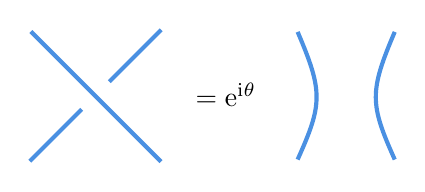
\begin{tikzpicture}[x=0.75pt,y=0.75pt,yscale=-1,xscale=1]
                %uncomment if require: \path (0,68); %set diagram left start at 0, and has height of 68
                
                %Straight Lines [id:da12351686453929012] 
                \draw [color={rgb, 255:red, 74; green, 144; blue, 226 }  ,draw opacity=1 ][line width=1.5]    (240.67,3.65) -- (303.37,66.35) ;
                %Straight Lines [id:da5675480043864236] 
                \draw [color={rgb, 255:red, 74; green, 144; blue, 226 }  ,draw opacity=1 ][line width=1.5]    (278.45,27.79) -- (303.45,2.79) ;
                %Straight Lines [id:da37770163193150785] 
                \draw [color={rgb, 255:red, 74; green, 144; blue, 226 }  ,draw opacity=1 ][line width=1.5]    (240.11,66.12) -- (265.11,41.12) ;
                
                %Curve Lines [id:da4265407093388114] 
                \draw [color={rgb, 255:red, 74; green, 144; blue, 226 }  ,draw opacity=1 ][line width=1.5]    (369.17,3.82) .. controls (381.5,32.65) and (381.17,38.65) .. (369.17,65.32) ;
                %Curve Lines [id:da5245986537990159] 
                \draw [color={rgb, 255:red, 74; green, 144; blue, 226 }  ,draw opacity=1 ][line width=1.5]    (415.96,3.82) .. controls (403.63,32.65) and (403.96,38.65) .. (415.96,65.32) ;
                
                
                % Text Node
                \draw (318.81,27.07) node [anchor=north west][inner sep=0.75pt]    {$=\mathrm{e}^{\mathrm{i} \theta }$};
        \end{tikzpicture}
        \caption{For abelian anyons, exchange gives a phase $\mathrm{e}^{\mathrm{i} \theta }$.}
        \label{fig:AbelianAnyonExchange}
\end{figure}

\begin{enumerate}
        \item For $A=\pm \mathrm{e}^{\mathrm{i} \pi /3}$ (and the complex conjugates of these values), show that the anyons are bosons or fermions respectively (i.e., $\mathrm{e}^{\mathrm{i} \theta } =\pm 1$ ).
        \item For $A=\pm \mathrm{e}^{\mathrm{i} \pi /6}$ (and the complex conjugates of these values) show the anyons are semions (i.e., $\mathrm{e}^{\mathrm{i} \theta } =\pm \mathrm{i}$ ). In fact these are precisely the anyons that arise for the $\nu =1/2$ fractional quantum Hall effect of bosons (We will discuss this later in this book (See chapter 37). This particular phase of quantum Hall matter has been produced experimentally(Clark et al. [2020]), but only in very small puddles so far and it has not been possible to measure braiding statistics as of yet.
\end{enumerate}
HINT: For (a) and (b) show first the identity shown in Fig. \ref{fig:ExchangeBosonsOrFermions}.

If you can't figure it out, try evaluating the Kauffman bracket invariant for a few knots with these values of $A$ and see how the result arises.

\begin{figure}[h!]
        \centering
        \tikzset{every picture/.style={line width=0.75pt}} %set default line width to 0.75pt        
        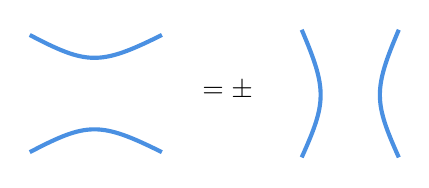
\begin{tikzpicture}[x=0.75pt,y=0.75pt,yscale=-1,xscale=1]
                %uncomment if require: \path (0,65); %set diagram left start at 0, and has height of 65
                %Curve Lines [id:da8961261533012252] 
                \draw [color={rgb, 255:red, 74; green, 144; blue, 226 }  ,draw opacity=1 ][line width=1.5]    (305.81,4.41) .. controls (275.96,19.3) and (269.75,18.9) .. (242.15,4.41) ;
                %Curve Lines [id:da47083895189428304] 
                \draw [color={rgb, 255:red, 74; green, 144; blue, 226 }  ,draw opacity=1 ][line width=1.5]    (305.81,60.89) .. controls (275.96,46.01) and (269.75,46.41) .. (242.15,60.89) ;
                
                %Curve Lines [id:da9898702962562469] 
                \draw [color={rgb, 255:red, 74; green, 144; blue, 226 }  ,draw opacity=1 ][line width=1.5]    (373.17,1.9) .. controls (385.5,30.74) and (385.17,36.74) .. (373.17,63.4) ;
                %Curve Lines [id:da26291761978783246] 
                \draw [color={rgb, 255:red, 74; green, 144; blue, 226 }  ,draw opacity=1 ][line width=1.5]    (419.96,1.9) .. controls (407.63,30.74) and (407.96,36.74) .. (419.96,63.4) ;
                % Text Node
                \draw (324,25.65) node [anchor=north west][inner sep=0.75pt]    {$=\pm $};
        \end{tikzpicture}
        \caption{For bosons or fermions the sign in this figure is $+$, for semions the sign is $-$.}
        \label{fig:ExchangeBosonsOrFermions}
\end{figure}

\paragraph{Answer}
Using the definition of Kauffman bracket:
\begin{equation*}
        \begin{aligned}
                \tikzset{every picture/.style={line width=0.75pt}} %set default line width to 0.75pt 
                
\begin{tikzpicture}[x=0.75pt,y=0.75pt,yscale=-1,xscale=1, baseline=(XXXX.south) ]
                        \path (0,68);\path (68.99652099609375,0);\draw    ($(current bounding box.center)+(0,0.3em)$) node [anchor=south] (XXXX) {};
                        %Straight Lines [id:da5470670447844541] 
                        \draw [color={rgb, 255:red, 74; green, 144; blue, 226 }  ,draw opacity=1 ][line width=1.5]    (3.67,4) -- (66.37,66.7) ;
                        %Straight Lines [id:da013140972627327496] 
                        \draw [color={rgb, 255:red, 74; green, 144; blue, 226 }  ,draw opacity=1 ][line width=1.5]    (41.45,28.14) -- (66.45,3.14) ;
                        %Straight Lines [id:da8599231631706779] 
                        \draw [color={rgb, 255:red, 74; green, 144; blue, 226 }  ,draw opacity=1 ][line width=1.5]    (3.11,66.47) -- (28.11,41.47) ;
                \end{tikzpicture}       
                & =A\tikzset{every picture/.style={line width=0.75pt}} %set default line width to 0.75pt        
                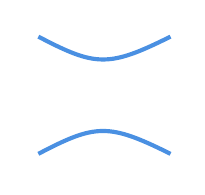
\begin{tikzpicture}[x=0.75pt,y=0.75pt,yscale=-1,xscale=1, baseline=(XXXX.south) ]
                        \path (0,67);\path (71.98169708251953,0);\draw    ($(current bounding box.center)+(0,0.3em)$) node [anchor=south] (XXXX) {};
                        %Curve Lines [id:da8933911166454194] 
                        \draw [color={rgb, 255:red, 74; green, 144; blue, 226 }  ,draw opacity=1 ][line width=1.5]    (68.81,4.31) .. controls (38.96,19.2) and (32.75,18.79) .. (5.15,4.31) ;
                        %Curve Lines [id:da4551593879680247] 
                        \draw [color={rgb, 255:red, 74; green, 144; blue, 226 }  ,draw opacity=1 ][line width=1.5]    (68.81,60.79) .. controls (38.96,45.9) and (32.75,46.3) .. (5.15,60.79) ;
                \end{tikzpicture}
                +A^{-1}\tikzset{every picture/.style={line width=0.75pt}} %set default line width to 0.75pt        
                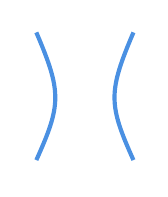
\begin{tikzpicture}[x=0.75pt,y=0.75pt,yscale=-1,xscale=1, baseline=(XXXX.south) ]
                        \path (0,68);\path (53.991668701171875,0);\draw    ($(current bounding box.center)+(0,0.3em)$) node [anchor=south] (XXXX) {};
                        %Curve Lines [id:da7648739395234672] 
                        \draw [color={rgb, 255:red, 74; green, 144; blue, 226 }  ,draw opacity=1 ][line width=1.5]    (4.17,2.29) .. controls (16.5,31.12) and (16.17,37.12) .. (4.17,63.79) ;
                        %Curve Lines [id:da5044659836989394] 
                        \draw [color={rgb, 255:red, 74; green, 144; blue, 226 }  ,draw opacity=1 ][line width=1.5]    (50.96,2.29) .. controls (38.63,31.12) and (38.96,37.12) .. (50.96,63.79) ;
                \end{tikzpicture}
                \\
                & \stackrel{!}{=}\mathrm{e}^{\mathrm{i} \theta }\tikzset{every picture/.style={line width=0.75pt}} %set default line width to 0.75pt        
                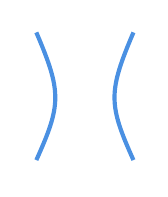
\begin{tikzpicture}[x=0.75pt,y=0.75pt,yscale=-1,xscale=1, baseline=(XXXX.south) ]
                        \path (0,68);\path (53.991668701171875,0);\draw    ($(current bounding box.center)+(0,0.3em)$) node [anchor=south] (XXXX) {};
                        %Curve Lines [id:da48143120116797333] 
                        \draw [color={rgb, 255:red, 74; green, 144; blue, 226 }  ,draw opacity=1 ][line width=1.5]    (4.17,2.29) .. controls (16.5,31.12) and (16.17,37.12) .. (4.17,63.79) ;
                        %Curve Lines [id:da5734280588341469] 
                        \draw [color={rgb, 255:red, 74; green, 144; blue, 226 }  ,draw opacity=1 ][line width=1.5]    (50.96,2.29) .. controls (38.63,31.12) and (38.96,37.12) .. (50.96,63.79) ;
                \end{tikzpicture}
                ,
        \end{aligned}
\end{equation*}
which means we have:
\begin{equation*}
        \tikzset{every picture/.style={line width=0.75pt}} %set default line width to 0.75pt        
        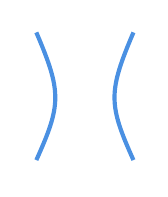
\begin{tikzpicture}[x=0.75pt,y=0.75pt,yscale=-1,xscale=1, baseline=(XXXX.south) ]
                \path (0,68);\path (53.991668701171875,0);\draw    ($(current bounding box.center)+(0,0.3em)$) node [anchor=south] (XXXX) {};
                %Curve Lines [id:da3520499283776384] 
                \draw [color={rgb, 255:red, 74; green, 144; blue, 226 }  ,draw opacity=1 ][line width=1.5]    (4.17,2.29) .. controls (16.5,31.12) and (16.17,37.12) .. (4.17,63.79) ;
                %Curve Lines [id:da7874206506093477] 
                \draw [color={rgb, 255:red, 74; green, 144; blue, 226 }  ,draw opacity=1 ][line width=1.5]    (50.96,2.29) .. controls (38.63,31.12) and (38.96,37.12) .. (50.96,63.79) ;
        \end{tikzpicture}
        =A^{-1}(\mathrm{e}^{\mathrm{i} \theta } -A^{-1})\tikzset{every picture/.style={line width=0.75pt}} %set default line width to 0.75pt        
        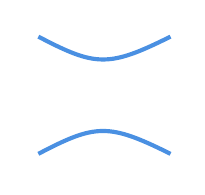
\begin{tikzpicture}[x=0.75pt,y=0.75pt,yscale=-1,xscale=1, baseline=(XXXX.south) ]
                \path (0,67);\path (71.98169708251953,0);\draw    ($(current bounding box.center)+(0,0.3em)$) node [anchor=south] (XXXX) {};
                %Curve Lines [id:da9101758088105385] 
                \draw [color={rgb, 255:red, 74; green, 144; blue, 226 }  ,draw opacity=1 ][line width=1.5]    (68.81,4.31) .. controls (38.96,19.2) and (32.75,18.79) .. (5.15,4.31) ;
                %Curve Lines [id:da9071304110135325] 
                \draw [color={rgb, 255:red, 74; green, 144; blue, 226 }  ,draw opacity=1 ][line width=1.5]    (68.81,60.79) .. controls (38.96,45.9) and (32.75,46.3) .. (5.15,60.79) ;
        \end{tikzpicture}
        .
\end{equation*}
At the same time, we also have
\begin{equation*}
        \begin{aligned}
                \tikzset{every picture/.style={line width=0.75pt}} %set default line width to 0.75pt        
                
\begin{tikzpicture}[x=0.75pt,y=0.75pt,yscale=-1,xscale=1, baseline=(XXXX.south) ]
                        \path (0,68);\path (68.99652099609375,0);\draw    ($(current bounding box.center)+(0,0.3em)$) node [anchor=south] (XXXX) {};
                        %Straight Lines [id:da7539388624541459] 
                        \draw [color={rgb, 255:red, 74; green, 144; blue, 226 }  ,draw opacity=1 ][line width=1.5]    (65.7,3.81) -- (3,66.51) ;
                        %Straight Lines [id:da3938438906428654] 
                        \draw [color={rgb, 255:red, 74; green, 144; blue, 226 }  ,draw opacity=1 ][line width=1.5]    (41.56,41.59) -- (66.56,66.59) ;
                        %Straight Lines [id:da18516570828706413] 
                        \draw [color={rgb, 255:red, 74; green, 144; blue, 226 }  ,draw opacity=1 ][line width=1.5]    (3.23,3.25) -- (28.23,28.25) ;
                \end{tikzpicture}
                & =A\tikzset{every picture/.style={line width=0.75pt}} %set default line width to 0.75pt        
                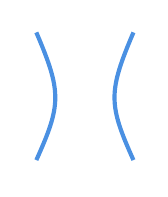
\begin{tikzpicture}[x=0.75pt,y=0.75pt,yscale=-1,xscale=1, baseline=(XXXX.south) ]
                        \path (0,68);\path (53.991668701171875,0);\draw    ($(current bounding box.center)+(0,0.3em)$) node [anchor=south] (XXXX) {};
                        %Curve Lines [id:da37581413358541704] 
                        \draw [color={rgb, 255:red, 74; green, 144; blue, 226 }  ,draw opacity=1 ][line width=1.5]    (4.17,2.29) .. controls (16.5,31.12) and (16.17,37.12) .. (4.17,63.79) ;
                        %Curve Lines [id:da9006964162238551] 
                        \draw [color={rgb, 255:red, 74; green, 144; blue, 226 }  ,draw opacity=1 ][line width=1.5]    (50.96,2.29) .. controls (38.63,31.12) and (38.96,37.12) .. (50.96,63.79) ;
                \end{tikzpicture}
                +A^{-1}\tikzset{every picture/.style={line width=0.75pt}} %set default line width to 0.75pt        
                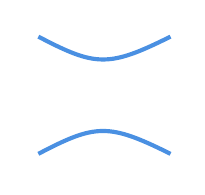
\begin{tikzpicture}[x=0.75pt,y=0.75pt,yscale=-1,xscale=1, baseline=(XXXX.south) ]
                        \path (0,67);\path (71.98169708251953,0);\draw    ($(current bounding box.center)+(0,0.3em)$) node [anchor=south] (XXXX) {};
                        %Curve Lines [id:da0002888383512205106] 
                        \draw [color={rgb, 255:red, 74; green, 144; blue, 226 }  ,draw opacity=1 ][line width=1.5]    (68.81,4.31) .. controls (38.96,19.2) and (32.75,18.79) .. (5.15,4.31) ;
                        %Curve Lines [id:da2642472194401073] 
                        \draw [color={rgb, 255:red, 74; green, 144; blue, 226 }  ,draw opacity=1 ][line width=1.5]    (68.81,60.79) .. controls (38.96,45.9) and (32.75,46.3) .. (5.15,60.79) ;
                \end{tikzpicture}
                \\
                & \stackrel{!}{=}\mathrm{e}^{-\mathrm{i} \theta }\tikzset{every picture/.style={line width=0.75pt}} %set default line width to 0.75pt        
                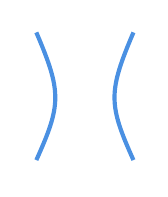
\begin{tikzpicture}[x=0.75pt,y=0.75pt,yscale=-1,xscale=1, baseline=(XXXX.south) ]
                        \path (0,68);\path (53.991668701171875,0);\draw    ($(current bounding box.center)+(0,0.3em)$) node [anchor=south] (XXXX) {};
                        %Curve Lines [id:da5214125017288944] 
                        \draw [color={rgb, 255:red, 74; green, 144; blue, 226 }  ,draw opacity=1 ][line width=1.5]    (4.17,2.29) .. controls (16.5,31.12) and (16.17,37.12) .. (4.17,63.79) ;
                        %Curve Lines [id:da2916432495183652] 
                        \draw [color={rgb, 255:red, 74; green, 144; blue, 226 }  ,draw opacity=1 ][line width=1.5]    (50.96,2.29) .. controls (38.63,31.12) and (38.96,37.12) .. (50.96,63.79) ;
                \end{tikzpicture}
                ,
        \end{aligned}        
\end{equation*}
Because exchange two particles in one certain direction gives a phase factor $\mathrm{e}^{\mathrm{i} \theta }$. Then
\begin{equation*}
        \tikzset{every picture/.style={line width=0.75pt}} %set default line width to 0.75pt        
        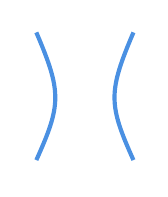
\begin{tikzpicture}[x=0.75pt,y=0.75pt,yscale=-1,xscale=1, baseline=(XXXX.south) ]
                \path (0,68);\path (53.991668701171875,0);\draw    ($(current bounding box.center)+(0,0.3em)$) node [anchor=south] (XXXX) {};
                %Curve Lines [id:da3082007174180428] 
                \draw [color={rgb, 255:red, 74; green, 144; blue, 226 }  ,draw opacity=1 ][line width=1.5]    (4.17,2.29) .. controls (16.5,31.12) and (16.17,37.12) .. (4.17,63.79) ;
                %Curve Lines [id:da2760148242111715] 
                \draw [color={rgb, 255:red, 74; green, 144; blue, 226 }  ,draw opacity=1 ][line width=1.5]    (50.96,2.29) .. controls (38.63,31.12) and (38.96,37.12) .. (50.96,63.79) ;
        \end{tikzpicture}
        =A(\mathrm{e}^{-\mathrm{i} \theta } -A)\tikzset{every picture/.style={line width=0.75pt}} %set default line width to 0.75pt        
        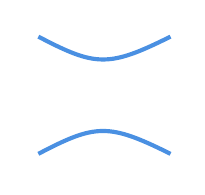
\begin{tikzpicture}[x=0.75pt,y=0.75pt,yscale=-1,xscale=1, baseline=(XXXX.south) ]
                \path (0,67);\path (71.98169708251953,0);\draw    ($(current bounding box.center)+(0,0.3em)$) node [anchor=south] (XXXX) {};
                %Curve Lines [id:da06451084320784006] 
                \draw [color={rgb, 255:red, 74; green, 144; blue, 226 }  ,draw opacity=1 ][line width=1.5]    (68.81,4.31) .. controls (38.96,19.2) and (32.75,18.79) .. (5.15,4.31) ;
                %Curve Lines [id:da13449620146904073] 
                \draw [color={rgb, 255:red, 74; green, 144; blue, 226 }  ,draw opacity=1 ][line width=1.5]    (68.81,60.79) .. controls (38.96,45.9) and (32.75,46.3) .. (5.15,60.79) ;
        \end{tikzpicture}
        .
\end{equation*}
So we have the equation
\begin{equation*}
        A(\mathrm{e}^{-\mathrm{i} \theta } -A) =A^{-1}({\mathrm{e}^{\mathrm{i} \theta } -A^{-1}}) \Rightarrow \mathrm{e}^{\mathrm{i} \theta } =-A^{3} \text{ or } A^{-1}.
\end{equation*}
Where $A^{-1}$ is a trivial solution. By the way, we also have
\begin{equation*}
        \tikzset{every picture/.style={line width=0.75pt}} %set default line width to 0.75pt        
        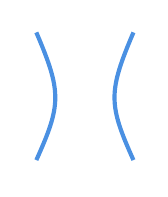
\begin{tikzpicture}[x=0.75pt,y=0.75pt,yscale=-1,xscale=1, baseline=(XXXX.south) ]
                \path (0,68);\path (53.991668701171875,0);\draw    ($(current bounding box.center)+(0,0.3em)$) node [anchor=south] (XXXX) {};
                %Curve Lines [id:da280533134954952] 
                \draw [color={rgb, 255:red, 74; green, 144; blue, 226 }  ,draw opacity=1 ][line width=1.5]    (4.17,2.29) .. controls (16.5,31.12) and (16.17,37.12) .. (4.17,63.79) ;
                %Curve Lines [id:da7685079345425179] 
                \draw [color={rgb, 255:red, 74; green, 144; blue, 226 }  ,draw opacity=1 ][line width=1.5]    (50.96,2.29) .. controls (38.63,31.12) and (38.96,37.12) .. (50.96,63.79) ;
        \end{tikzpicture}
        =-\frac{A^{2}}{1+A^{4}}\tikzset{every picture/.style={line width=0.75pt}} %set default line width to 0.75pt        
        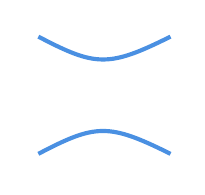
\begin{tikzpicture}[x=0.75pt,y=0.75pt,yscale=-1,xscale=1, baseline=(XXXX.south) ]
                \path (0,67);\path (71.98169708251953,0);\draw    ($(current bounding box.center)+(0,0.3em)$) node [anchor=south] (XXXX) {};
                %Curve Lines [id:da7107080303425743] 
                \draw [color={rgb, 255:red, 74; green, 144; blue, 226 }  ,draw opacity=1 ][line width=1.5]    (68.81,4.31) .. controls (38.96,19.2) and (32.75,18.79) .. (5.15,4.31) ;
                %Curve Lines [id:da4726019052110213] 
                \draw [color={rgb, 255:red, 74; green, 144; blue, 226 }  ,draw opacity=1 ][line width=1.5]    (68.81,60.79) .. controls (38.96,45.9) and (32.75,46.3) .. (5.15,60.79) ;
        \end{tikzpicture}
        .
\end{equation*}

(a) For $A=\pm \mathrm{e}^{\mathrm{i} \pi /3}$, we have
\begin{equation*}
        \mathrm{e}^{\mathrm{i} \theta } =\pm 1,
\end{equation*}
which gives bosons for fermions. And
\begin{equation}\label{fermions}
        \tikzset{every picture/.style={line width=0.75pt}} %set default line width to 0.75pt        
        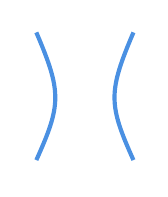
\begin{tikzpicture}[x=0.75pt,y=0.75pt,yscale=-1,xscale=1, baseline=(XXXX.south) ]
                \path (0,68);\path (53.991668701171875,0);\draw    ($(current bounding box.center)+(0,0.3em)$) node [anchor=south] (XXXX) {};
                %Curve Lines [id:da48157044438828867] 
                \draw [color={rgb, 255:red, 74; green, 144; blue, 226 }  ,draw opacity=1 ][line width=1.5]    (4.17,2.29) .. controls (16.5,31.12) and (16.17,37.12) .. (4.17,63.79) ;
                %Curve Lines [id:da8477956884783802] 
                \draw [color={rgb, 255:red, 74; green, 144; blue, 226 }  ,draw opacity=1 ][line width=1.5]    (50.96,2.29) .. controls (38.63,31.12) and (38.96,37.12) .. (50.96,63.79) ;
        \end{tikzpicture}
        =\tikzset{every picture/.style={line width=0.75pt}} %set default line width to 0.75pt        
        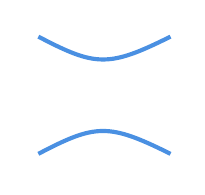
\begin{tikzpicture}[x=0.75pt,y=0.75pt,yscale=-1,xscale=1, baseline=(XXXX.south) ]
                \path (0,67);\path (71.98169708251953,0);\draw    ($(current bounding box.center)+(0,0.3em)$) node [anchor=south] (XXXX) {};
                %Curve Lines [id:da6857291636967586] 
                \draw [color={rgb, 255:red, 74; green, 144; blue, 226 }  ,draw opacity=1 ][line width=1.5]    (68.81,4.31) .. controls (38.96,19.2) and (32.75,18.79) .. (5.15,4.31) ;
                %Curve Lines [id:da8898537612520505] 
                \draw [color={rgb, 255:red, 74; green, 144; blue, 226 }  ,draw opacity=1 ][line width=1.5]    (68.81,60.79) .. controls (38.96,45.9) and (32.75,46.3) .. (5.15,60.79) ;
        \end{tikzpicture}
        ,
\end{equation}
which are fermions and bosons. 

(b) For $A=\pm \mathrm{e}^{\mathrm{i} \pi /6}$, we have
\begin{equation*}
        \mathrm{e}^{\mathrm{i} \theta } =\mp \mathrm{i} ,
\end{equation*}
which gives semions. And
\begin{equation}\label{semions}
        \tikzset{every picture/.style={line width=0.75pt}} %set default line width to 0.75pt        
        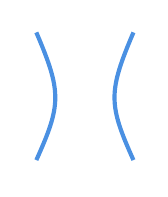
\begin{tikzpicture}[x=0.75pt,y=0.75pt,yscale=-1,xscale=1, baseline=(XXXX.south) ]
                \path (0,68);\path (53.991668701171875,0);\draw    ($(current bounding box.center)+(0,0.3em)$) node [anchor=south] (XXXX) {};
                %Curve Lines [id:da7554397487746631] 
                \draw [color={rgb, 255:red, 74; green, 144; blue, 226 }  ,draw opacity=1 ][line width=1.5]    (4.17,2.29) .. controls (16.5,31.12) and (16.17,37.12) .. (4.17,63.79) ;
                %Curve Lines [id:da9971387307406114] 
                \draw [color={rgb, 255:red, 74; green, 144; blue, 226 }  ,draw opacity=1 ][line width=1.5]    (50.96,2.29) .. controls (38.63,31.12) and (38.96,37.12) .. (50.96,63.79) ;
        \end{tikzpicture}
        =-\tikzset{every picture/.style={line width=0.75pt}} %set default line width to 0.75pt        
        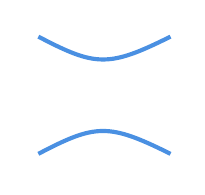
\begin{tikzpicture}[x=0.75pt,y=0.75pt,yscale=-1,xscale=1, baseline=(XXXX.south) ]
                \path (0,67);\path (71.98169708251953,0);\draw    ($(current bounding box.center)+(0,0.3em)$) node [anchor=south] (XXXX) {};
                %Curve Lines [id:da5892182617723671] 
                \draw [color={rgb, 255:red, 74; green, 144; blue, 226 }  ,draw opacity=1 ][line width=1.5]    (68.81,4.31) .. controls (38.96,19.2) and (32.75,18.79) .. (5.15,4.31) ;
                %Curve Lines [id:da7044992807132684] 
                \draw [color={rgb, 255:red, 74; green, 144; blue, 226 }  ,draw opacity=1 ][line width=1.5]    (68.81,60.79) .. controls (38.96,45.9) and (32.75,46.3) .. (5.15,60.79) ;
        \end{tikzpicture}
        ,
\end{equation}
which are semions. 

Such illustration can also be viewed as if we first acknowledge equ.~\ref{fermions} and equ.~\ref{semions}, then $A=\pm \mathrm{e}^{\mathrm{i}\pi/3}$ will give $A^2+A^{-2}=\pm 1$, and $A=\pm \mathrm{e}^{\mathrm{i}\pi/6}$ will give $A^2-A^{-2}=\pm \mathrm{i}$.

\section{Reidermeister moves and the Kauffman Bracket}
Show that the Kauffman bracket invariant is unchanged under application of Reidermeister move of type II and type III. Thus conclude that the Kauffman invariant is an invariant of regular isotopy.

\paragraph{Answer}
(a) The Reidermeister move of type II is given by Fig.\ref{fig:ReidermeisterMoveOfTypeII}.
\begin{figure}[h!]
        \centering
        \tikzset{every picture/.style={line width=0.75pt}} %set default line width to 0.75pt        
        
        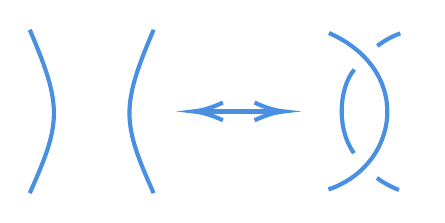
\begin{tikzpicture}[x=0.75pt,y=0.75pt,yscale=-1,xscale=1]
                %uncomment if require: \path (0,82); %set diagram left start at 0, and has height of 82
                
                %Curve Lines [id:da28666373624741825] 
                \draw [color={rgb, 255:red, 74; green, 144; blue, 226 }  ,draw opacity=1 ][line width=1.5]    (231.17,1.01) .. controls (246.9,37.91) and (246.47,45.59) .. (231.17,79.72) ;
                %Curve Lines [id:da6473636293749112] 
                \draw [color={rgb, 255:red, 74; green, 144; blue, 226 }  ,draw opacity=1 ][line width=1.5]    (290.85,1.01) .. controls (275.12,37.91) and (275.54,45.59) .. (290.85,79.72) ;
                
                %Curve Lines [id:da34726741926398463] 
                \draw [color={rgb, 255:red, 74; green, 144; blue, 226 }  ,draw opacity=1 ][line width=1.5]    (375.31,2.56) .. controls (416.46,20.8) and (409.06,66.44) .. (375.08,77.96) ;
                %Curve Lines [id:da9780689263100604] 
                \draw [color={rgb, 255:red, 74; green, 144; blue, 226 }  ,draw opacity=1 ][line width=1.5]    (409.7,2.77) .. controls (405.6,4.17) and (401.2,6.73) .. (398.66,8.86) ;
                %Curve Lines [id:da16670674465631863] 
                \draw [color={rgb, 255:red, 74; green, 144; blue, 226 }  ,draw opacity=1 ][line width=1.5]    (398.43,72.41) .. controls (401.9,74.97) and (406.06,77.1) .. (409.06,78.17) ;
                %Curve Lines [id:da3643115225934235] 
                \draw [color={rgb, 255:red, 74; green, 144; blue, 226 }  ,draw opacity=1 ][line width=1.5]    (387.56,20.16) .. controls (380.4,28.55) and (378.55,48.1) .. (387.33,60.47) ;
                
                %Straight Lines [id:da4458936620449674] 
                \draw [color={rgb, 255:red, 74; green, 144; blue, 226 }  ,draw opacity=1 ][line width=1.5]    (313,40.36) -- (350.7,40.36) ;
                \draw [shift={(353.7,40.36)}, rotate = 180] [color={rgb, 255:red, 74; green, 144; blue, 226 }  ,draw opacity=1 ][line width=1.5]    (14.21,-4.28) .. controls (9.04,-1.82) and (4.3,-0.39) .. (0,0) .. controls (4.3,0.39) and (9.04,1.82) .. (14.21,4.28)   ;
                \draw [shift={(310,40.36)}, rotate = 0] [color={rgb, 255:red, 74; green, 144; blue, 226 }  ,draw opacity=1 ][line width=1.5]    (14.21,-4.28) .. controls (9.04,-1.82) and (4.3,-0.39) .. (0,0) .. controls (4.3,0.39) and (9.04,1.82) .. (14.21,4.28)   ;
        \end{tikzpicture}
        \caption{Reidermeister move of type II}
        \label{fig:ReidermeisterMoveOfTypeII}
\end{figure}
Then according to the definition of the Kauffman bracket, we have:
\begin{equation*}
        \begin{aligned}
                \tikzset{every picture/.style={line width=0.75pt}} %set default line width to 0.75pt        
                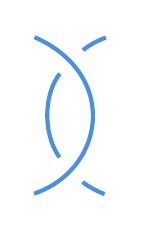
\begin{tikzpicture}[x=0.75pt,y=0.75pt,yscale=-1,xscale=1, baseline=(XXXX.south) ]
                        \path (0,83);\path (40.99652099609375,0);\draw    ($(current bounding box.center)+(0,0.3em)$) node [anchor=south] (XXXX) {};
                        %Curve Lines [id:da9604095537894752] 
                        \draw [color={rgb, 255:red, 74; green, 144; blue, 226 }  ,draw opacity=1 ][line width=1.5]    (3.31,4.56) .. controls (44.46,22.8) and (37.06,68.44) .. (3.08,79.96) ;
                        %Curve Lines [id:da44353755004889783] 
                        \draw [color={rgb, 255:red, 74; green, 144; blue, 226 }  ,draw opacity=1 ][line width=1.5]    (37.7,4.77) .. controls (33.6,6.17) and (29.2,8.73) .. (26.66,10.86) ;
                        %Curve Lines [id:da9884546368227021] 
                        \draw [color={rgb, 255:red, 74; green, 144; blue, 226 }  ,draw opacity=1 ][line width=1.5]    (26.43,74.41) .. controls (29.9,76.97) and (34.06,79.1) .. (37.06,80.17) ;
                        %Curve Lines [id:da1642034829302086] 
                        \draw [color={rgb, 255:red, 74; green, 144; blue, 226 }  ,draw opacity=1 ][line width=1.5]    (15.56,22.16) .. controls (8.4,30.55) and (6.55,50.1) .. (15.33,62.47) ;
                \end{tikzpicture}
                & =A\tikzset{every picture/.style={line width=0.75pt}} %set default line width to 0.75pt        
                
\begin{tikzpicture}[x=0.75pt,y=0.75pt,yscale=-1,xscale=1, baseline=(XXXX.south) ]
                        \path (0,92);\path (50.99652099609375,0);\draw    ($(current bounding box.center)+(0,0.3em)$) node [anchor=south] (XXXX) {};
                        %Curve Lines [id:da6343061819532925] 
                        \draw [color={rgb, 255:red, 74; green, 144; blue, 226 }  ,draw opacity=1 ][line width=1.5]    (48.86,3.92) .. controls (27.16,14.74) and (22.64,14.45) .. (2.57,3.92) ;
                        %Straight Lines [id:da10138287838463445] 
                        \draw [color={rgb, 255:red, 74; green, 144; blue, 226 }  ,draw opacity=1 ][line width=1.5]    (30.64,71.36) -- (48.82,89.54) ;
                        %Curve Lines [id:da8125503416637623] 
                        \draw [color={rgb, 255:red, 74; green, 144; blue, 226 }  ,draw opacity=1 ][line width=1.5]    (20.95,61.67) .. controls (13.06,53.79) and (8.33,48.34) .. (2.78,43.5) .. controls (2.88,15.63) and (47.22,12.36) .. (48.19,43.9) .. controls (39.59,52.34) and (12.69,78.88) .. (2.61,89.48) ;
                \end{tikzpicture}
                +A^{-1}\tikzset{every picture/.style={line width=0.75pt}} %set default line width to 0.75pt        
                
\begin{tikzpicture}[x=0.75pt,y=0.75pt,yscale=-1,xscale=1, baseline=(XXXX.south) ]
                        \path (0,68);\path (68.99652099609375,0);\draw    ($(current bounding box.center)+(0,0.3em)$) node [anchor=south] (XXXX) {};
                        %Straight Lines [id:da6104518270284445] 
                        \draw [color={rgb, 255:red, 74; green, 144; blue, 226 }  ,draw opacity=1 ][line width=1.5]    (65.7,3.81) -- (3,66.51) ;
                        %Straight Lines [id:da0766348817654059] 
                        \draw [color={rgb, 255:red, 74; green, 144; blue, 226 }  ,draw opacity=1 ][line width=1.5]    (41.56,41.59) -- (66.56,66.59) ;
                        %Straight Lines [id:da42798350857778145] 
                        \draw [color={rgb, 255:red, 74; green, 144; blue, 226 }  ,draw opacity=1 ][line width=1.5]    (3.23,3.25) -- (28.23,28.25) ;
                \end{tikzpicture}
                \\
                & =A \left( A\tikzset{every picture/.style={line width=0.75pt}} %set default line width to 0.75pt        
                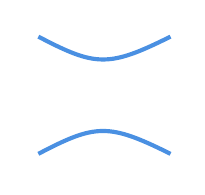
\begin{tikzpicture}[x=0.75pt,y=0.75pt,yscale=-1,xscale=1, baseline=(XXXX.south) ]
                        \path (0,67);\path (71.98169708251953,0);\draw    ($(current bounding box.center)+(0,0.3em)$) node [anchor=south] (XXXX) {};
                        %Curve Lines [id:da4627840070580258] 
                        \draw [color={rgb, 255:red, 74; green, 144; blue, 226 }  ,draw opacity=1 ][line width=1.5]    (68.81,4.31) .. controls (38.96,19.2) and (32.75,18.79) .. (5.15,4.31) ;
                        %Curve Lines [id:da7914769351421946] 
                        \draw [color={rgb, 255:red, 74; green, 144; blue, 226 }  ,draw opacity=1 ][line width=1.5]    (68.81,60.79) .. controls (38.96,45.9) and (32.75,46.3) .. (5.15,60.79) ;
                \end{tikzpicture} 
                +A^{-1}\tikzset{every picture/.style={line width=0.75pt}} %set default line width to 0.75pt        
                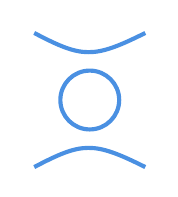
\begin{tikzpicture}[x=0.75pt,y=0.75pt,yscale=-1,xscale=1, baseline=(XXXX.south) ]
                        \path (0,68);\path (58.99652099609375,0);\draw    ($(current bounding box.center)+(0,0.3em)$) node [anchor=south] (XXXX) {};
                        %Curve Lines [id:da912568481834767] 
                        \draw [color={rgb, 255:red, 74; green, 144; blue, 226 }  ,draw opacity=1 ][line width=1.5]    (56.68,2.54) .. controls (31.58,15.06) and (26.36,14.72) .. (3.15,2.54) ;
                        %Curve Lines [id:da17235049610260633] 
                        \draw [color={rgb, 255:red, 74; green, 144; blue, 226 }  ,draw opacity=1 ][line width=1.5]    (56.68,67.17) .. controls (31.58,54.65) and (26.36,54.99) .. (3.15,67.17) ;
                        %Shape: Ellipse [id:dp9280843921436426] 
                        \draw  [color={rgb, 255:red, 74; green, 144; blue, 226 }  ,draw opacity=1 ][line width=1.5]  (15.74,34.85) .. controls (15.74,27.02) and (22.08,20.68) .. (29.91,20.68) .. controls (37.74,20.68) and (44.09,27.02) .. (44.09,34.85) .. controls (44.09,42.68) and (37.74,49.03) .. (29.91,49.03) .. controls (22.08,49.03) and (15.74,42.68) .. (15.74,34.85) -- cycle ;
                \end{tikzpicture}
                \right)
                +A^{-1}\left( A \tikzset{every picture/.style={line width=0.75pt}} %set default line width to 0.75pt        
                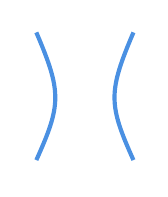
\begin{tikzpicture}[x=0.75pt,y=0.75pt,yscale=-1,xscale=1, baseline=(XXXX.south) ]
                        \path (0,68);\path (53.991668701171875,0);\draw    ($(current bounding box.center)+(0,0.3em)$) node [anchor=south] (XXXX) {};
                        %Curve Lines [id:da296212719001264] 
                        \draw [color={rgb, 255:red, 74; green, 144; blue, 226 }  ,draw opacity=1 ][line width=1.5]    (4.17,2.29) .. controls (16.5,31.12) and (16.17,37.12) .. (4.17,63.79) ;
                        %Curve Lines [id:da14704308294878077] 
                        \draw [color={rgb, 255:red, 74; green, 144; blue, 226 }  ,draw opacity=1 ][line width=1.5]    (50.96,2.29) .. controls (38.63,31.12) and (38.96,37.12) .. (50.96,63.79) ;
                \end{tikzpicture}
                +A^{-1}\tikzset{every picture/.style={line width=0.75pt}} %set default line width to 0.75pt        
                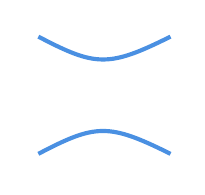
\begin{tikzpicture}[x=0.75pt,y=0.75pt,yscale=-1,xscale=1, baseline=(XXXX.south) ]
                        \path (0,67);\path (71.98169708251953,0);\draw    ($(current bounding box.center)+(0,0.3em)$) node [anchor=south] (XXXX) {};
                        %Curve Lines [id:da12181300195230782] 
                        \draw [color={rgb, 255:red, 74; green, 144; blue, 226 }  ,draw opacity=1 ][line width=1.5]    (68.81,4.31) .. controls (38.96,19.2) and (32.75,18.79) .. (5.15,4.31) ;
                        %Curve Lines [id:da003208814156384854] 
                        \draw [color={rgb, 255:red, 74; green, 144; blue, 226 }  ,draw opacity=1 ][line width=1.5]    (68.81,60.79) .. controls (38.96,45.9) and (32.75,46.3) .. (5.15,60.79) ;
                \end{tikzpicture}
                \right)\\
                & =A^{2}\tikzset{every picture/.style={line width=0.75pt}} %set default line width to 0.75pt        
                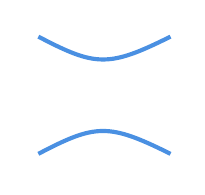
\begin{tikzpicture}[x=0.75pt,y=0.75pt,yscale=-1,xscale=1, baseline=(XXXX.south) ]
                        \path (0,67);\path (71.98169708251953,0);\draw    ($(current bounding box.center)+(0,0.3em)$) node [anchor=south] (XXXX) {};
                        %Curve Lines [id:da2751841456474464] 
                        \draw [color={rgb, 255:red, 74; green, 144; blue, 226 }  ,draw opacity=1 ][line width=1.5]    (68.81,4.31) .. controls (38.96,19.2) and (32.75,18.79) .. (5.15,4.31) ;
                        %Curve Lines [id:da28927063236750583] 
                        \draw [color={rgb, 255:red, 74; green, 144; blue, 226 }  ,draw opacity=1 ][line width=1.5]    (68.81,60.79) .. controls (38.96,45.9) and (32.75,46.3) .. (5.15,60.79) ;
                \end{tikzpicture}
                +\tikzset{every picture/.style={line width=0.75pt}} %set default line width to 0.75pt        
                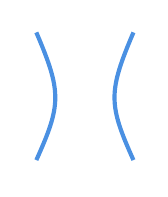
\begin{tikzpicture}[x=0.75pt,y=0.75pt,yscale=-1,xscale=1, baseline=(XXXX.south) ]
                        \path (0,68);\path (53.991668701171875,0);\draw    ($(current bounding box.center)+(0,0.3em)$) node [anchor=south] (XXXX) {};
                        %Curve Lines [id:da32898216042375594] 
                        \draw [color={rgb, 255:red, 74; green, 144; blue, 226 }  ,draw opacity=1 ][line width=1.5]    (4.17,2.29) .. controls (16.5,31.12) and (16.17,37.12) .. (4.17,63.79) ;
                        %Curve Lines [id:da2744164658246455] 
                        \draw [color={rgb, 255:red, 74; green, 144; blue, 226 }  ,draw opacity=1 ][line width=1.5]    (50.96,2.29) .. controls (38.63,31.12) and (38.96,37.12) .. (50.96,63.79) ;
                \end{tikzpicture}
                +d\tikzset{every picture/.style={line width=0.75pt}} %set default line width to 0.75pt        
                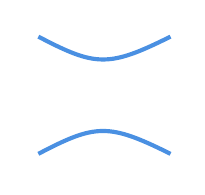
\begin{tikzpicture}[x=0.75pt,y=0.75pt,yscale=-1,xscale=1, baseline=(XXXX.south) ]
                        \path (0,67);\path (71.98169708251953,0);\draw    ($(current bounding box.center)+(0,0.3em)$) node [anchor=south] (XXXX) {};
                        %Curve Lines [id:da6870558472651833] 
                        \draw [color={rgb, 255:red, 74; green, 144; blue, 226 }  ,draw opacity=1 ][line width=1.5]    (68.81,4.31) .. controls (38.96,19.2) and (32.75,18.79) .. (5.15,4.31) ;
                        %Curve Lines [id:da13357681707506375] 
                        \draw [color={rgb, 255:red, 74; green, 144; blue, 226 }  ,draw opacity=1 ][line width=1.5]    (68.81,60.79) .. controls (38.96,45.9) and (32.75,46.3) .. (5.15,60.79) ;
                \end{tikzpicture}
                +A^{-2}\tikzset{every picture/.style={line width=0.75pt}} %set default line width to 0.75pt        
                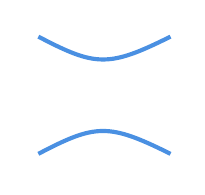
\begin{tikzpicture}[x=0.75pt,y=0.75pt,yscale=-1,xscale=1, baseline=(XXXX.south) ]
                        \path (0,67);\path (71.98169708251953,0);\draw    ($(current bounding box.center)+(0,0.3em)$) node [anchor=south] (XXXX) {};
                        %Curve Lines [id:da8617051673767433] 
                        \draw [color={rgb, 255:red, 74; green, 144; blue, 226 }  ,draw opacity=1 ][line width=1.5]    (68.81,4.31) .. controls (38.96,19.2) and (32.75,18.79) .. (5.15,4.31) ;
                        %Curve Lines [id:da5303437875908261] 
                        \draw [color={rgb, 255:red, 74; green, 144; blue, 226 }  ,draw opacity=1 ][line width=1.5]    (68.81,60.79) .. controls (38.96,45.9) and (32.75,46.3) .. (5.15,60.79) ;
                \end{tikzpicture}
                \\
                & =\tikzset{every picture/.style={line width=0.75pt}} %set default line width to 0.75pt        
                \begin{tikzpicture}[x=0.75pt,y=0.75pt,yscale=-1,xscale=1, baseline=(XXXX.south) ]
                        \path (0,68);\path (53.991668701171875,0);\draw    ($(current bounding box.center)+(0,0.3em)$) node [anchor=south] (XXXX) {};
                        %Curve Lines [id:da9892583999632016] 
                        \draw [color={rgb, 255:red, 74; green, 144; blue, 226 }  ,draw opacity=1 ][line width=1.5]    (4.17,2.29) .. controls (16.5,31.12) and (16.17,37.12) .. (4.17,63.79) ;
                        %Curve Lines [id:da9019420104276974] 
                        \draw [color={rgb, 255:red, 74; green, 144; blue, 226 }  ,draw opacity=1 ][line width=1.5]    (50.96,2.29) .. controls (38.63,31.12) and (38.96,37.12) .. (50.96,63.79) ;
                \end{tikzpicture}
                .
        \end{aligned}
\end{equation*}
In the last line we use $d=-A^{2} -A^{-2}$. Now we can see type II is invariant. 

(b) The Reidermeister move of type III is given by Fig.\ref{fig:ReidermeisterMoveOfTypeIII}.
\begin{figure}[h!]
        \centering
        \tikzset{every picture/.style={line width=0.75pt}} %set default line width to 0.75pt        
        
        \begin{tikzpicture}[x=0.75pt,y=0.75pt,yscale=-1,xscale=1]
                %uncomment if require: \path (0,83); %set diagram left start at 0, and has height of 83
                
                %Straight Lines [id:da11950785204529102] 
                \draw [color={rgb, 255:red, 74; green, 144; blue, 226 }  ,draw opacity=1 ][line width=1.5]    (313,40.77) -- (350.7,40.77) ;
                \draw [shift={(353.7,40.77)}, rotate = 180] [color={rgb, 255:red, 74; green, 144; blue, 226 }  ,draw opacity=1 ][line width=1.5]    (14.21,-4.28) .. controls (9.04,-1.82) and (4.3,-0.39) .. (0,0) .. controls (4.3,0.39) and (9.04,1.82) .. (14.21,4.28)   ;
                \draw [shift={(310,40.77)}, rotate = 0] [color={rgb, 255:red, 74; green, 144; blue, 226 }  ,draw opacity=1 ][line width=1.5]    (14.21,-4.28) .. controls (9.04,-1.82) and (4.3,-0.39) .. (0,0) .. controls (4.3,0.39) and (9.04,1.82) .. (14.21,4.28)   ;
                %Straight Lines [id:da8207765534905693] 
                \draw [color={rgb, 255:red, 74; green, 144; blue, 226 }  ,draw opacity=1 ][line width=1.5]    (229.76,4.84) -- (302.61,77.69) ;
                %Straight Lines [id:da43977309937961295] 
                \draw [color={rgb, 255:red, 74; green, 144; blue, 226 }  ,draw opacity=1 ][line width=1.5]    (273.65,32.88) -- (302.7,3.84) ;
                %Straight Lines [id:da7291965597075933] 
                \draw [color={rgb, 255:red, 74; green, 144; blue, 226 }  ,draw opacity=1 ][line width=1.5]    (229.11,77.43) -- (258.16,48.38) ;
                %Straight Lines [id:da9127752946580543] 
                \draw [color={rgb, 255:red, 74; green, 144; blue, 226 }  ,draw opacity=1 ][line width=1.5]    (251.18,4.66) -- (251.18,19.4) ;
                %Straight Lines [id:da5580787674820835] 
                \draw [color={rgb, 255:red, 74; green, 144; blue, 226 }  ,draw opacity=1 ][line width=1.5]    (251.18,32.2) -- (251.18,47.51) ;
                %Straight Lines [id:da5788807019103526] 
                \draw [color={rgb, 255:red, 74; green, 144; blue, 226 }  ,draw opacity=1 ][line width=1.5]    (251.18,61.42) -- (251.18,76.72) ;
                
                %Straight Lines [id:da1822021649397716] 
                \draw [color={rgb, 255:red, 74; green, 144; blue, 226 }  ,draw opacity=1 ][line width=1.5]    (359.42,5.16) -- (431.61,77.36) ;
                %Straight Lines [id:da719661142881121] 
                \draw [color={rgb, 255:red, 74; green, 144; blue, 226 }  ,draw opacity=1 ][line width=1.5]    (398.68,37.19) -- (431.7,4.17) ;
                %Straight Lines [id:da0823586599622459] 
                \draw [color={rgb, 255:red, 74; green, 144; blue, 226 }  ,draw opacity=1 ][line width=1.5]    (358.78,77.09) -- (391.3,44.58) ;
                %Straight Lines [id:da8525034743711262] 
                \draw [color={rgb, 255:red, 74; green, 144; blue, 226 }  ,draw opacity=1 ][line width=1.5]    (409.01,4.98) -- (409.01,19.6) ;
                %Straight Lines [id:da246160857461047] 
                \draw [color={rgb, 255:red, 74; green, 144; blue, 226 }  ,draw opacity=1 ][line width=1.5]    (409.01,32.28) -- (409.01,47.45) ;
                %Straight Lines [id:da5380394964109403] 
                \draw [color={rgb, 255:red, 74; green, 144; blue, 226 }  ,draw opacity=1 ][line width=1.5]    (409.01,61.23) -- (409.01,76.4) ;
        \end{tikzpicture}
        \caption{Reidermeister move of type III}
        \label{fig:ReidermeisterMoveOfTypeIII}
\end{figure}
Then according to the definition of the Kauffman bracket, we have:

\begin{align*}
                \tikzset{every picture/.style={line width=0.75pt}} %set default line width to 0.75pt        
                \begin{tikzpicture}[x=0.75pt,y=0.75pt,yscale=-1,xscale=1, baseline=(XXXX.south) ]
                        \path (0,79);\path (76.99652099609375,0);\draw    ($(current bounding box.center)+(0,0.3em)$) node [anchor=south] (XXXX) {};
                        %Straight Lines [id:da5322048377507285] 
                        \draw [color={rgb, 255:red, 74; green, 144; blue, 226 }  ,draw opacity=1 ][line width=1.5]    (2.76,3.84) -- (75.61,76.69) ;
                        %Straight Lines [id:da2834370641983299] 
                        \draw [color={rgb, 255:red, 74; green, 144; blue, 226 }  ,draw opacity=1 ][line width=1.5]    (46.65,31.88) -- (75.7,2.84) ;
                        %Straight Lines [id:da7335835078220603] 
                        \draw [color={rgb, 255:red, 74; green, 144; blue, 226 }  ,draw opacity=1 ][line width=1.5]    (2.11,76.43) -- (31.16,47.38) ;
                        %Straight Lines [id:da6290897514246225] 
                        \draw [color={rgb, 255:red, 74; green, 144; blue, 226 }  ,draw opacity=1 ][line width=1.5]    (24.18,3.66) -- (24.18,18.4) ;
                        %Straight Lines [id:da7855778727017275] 
                        \draw [color={rgb, 255:red, 74; green, 144; blue, 226 }  ,draw opacity=1 ][line width=1.5]    (24.18,31.2) -- (24.18,46.51) ;
                        %Straight Lines [id:da40285349600704823] 
                        \draw [color={rgb, 255:red, 74; green, 144; blue, 226 }  ,draw opacity=1 ][line width=1.5]    (24.18,60.42) -- (24.18,75.72) ;
                \end{tikzpicture}
                & =A \tikzset{every picture/.style={line width=0.75pt}} %set default line width to 0.75pt        
                \begin{tikzpicture}[x=0.75pt,y=0.75pt,yscale=-1,xscale=1, baseline=(XXXX.south) ]
                        \path (0,81);\path (79.99413299560547,0);\draw    ($(current bounding box.center)+(0,0.3em)$) node [anchor=south] (XXXX) {};
                        %Curve Lines [id:da9862043434565733] 
                        \draw [color={rgb, 255:red, 74; green, 144; blue, 226 }  ,draw opacity=1 ][line width=1.5]    (62.72,2.31) .. controls (37.09,15.09) and (31.75,14.75) .. (8.04,2.31) ;
                        %Straight Lines [id:da7232272884844684] 
                        \draw [color={rgb, 255:red, 74; green, 144; blue, 226 }  ,draw opacity=1 ][line width=1.5]    (47.49,38.48) -- (66.18,19.79) ;
                        %Straight Lines [id:da5625150004968165] 
                        \draw [color={rgb, 255:red, 74; green, 144; blue, 226 }  ,draw opacity=1 ][line width=1.5]    (7.51,79.11) -- (37.49,49.14) ;
                        %Straight Lines [id:da4800775441178744] 
                        \draw [color={rgb, 255:red, 74; green, 144; blue, 226 }  ,draw opacity=1 ][line width=1.5]    (30.59,66.9) -- (42.81,79.11) ;
                        %Curve Lines [id:da8772854853652521] 
                        \draw [color={rgb, 255:red, 74; green, 144; blue, 226 }  ,draw opacity=1 ][line width=1.5]    (18.66,56.27) .. controls (0.27,39.31) and (-2.34,26.91) .. (5.49,21.03) .. controls (13.32,15.16) and (21.8,22.34) .. (78.29,78.46) ;
                \end{tikzpicture}
                +A^{-1}\tikzset{every picture/.style={line width=0.75pt}} %set default line width to 0.75pt        
                \begin{tikzpicture}[x=0.75pt,y=0.75pt,yscale=-1,xscale=1, baseline=(XXXX.south) ]
                        \path (0,79);\path (97.99652099609375,0);\draw    ($(current bounding box.center)+(0,0.3em)$) node [anchor=south] (XXXX) {};
                        %Straight Lines [id:da651734203263048] 
                        \draw [color={rgb, 255:red, 74; green, 144; blue, 226 }  ,draw opacity=1 ][line width=1.5]    (22.94,1.73) -- (97.13,75.92) ;
                        %Straight Lines [id:da9822862230824239] 
                        \draw [color={rgb, 255:red, 74; green, 144; blue, 226 }  ,draw opacity=1 ][line width=1.5]    (58.66,25.97) -- (82,2.63) ;
                        %Straight Lines [id:da5738361847067126] 
                        \draw [color={rgb, 255:red, 74; green, 144; blue, 226 }  ,draw opacity=1 ][line width=1.5]    (8.71,76.73) -- (46.16,39.29) ;
                        %Straight Lines [id:da651347852864083] 
                        \draw [color={rgb, 255:red, 74; green, 144; blue, 226 }  ,draw opacity=1 ][line width=1.5]    (37.54,61.48) -- (52.8,76.73) ;
                        %Straight Lines [id:da16594256373987704] 
                        \draw [color={rgb, 255:red, 74; green, 144; blue, 226 }  ,draw opacity=1 ][line width=1.5]    (3.89,29.45) -- (22.64,48.2) ;
                \end{tikzpicture}
                \\
                & =A\left(A \tikzset{every picture/.style={line width=0.75pt}} %set default line width to 0.75pt        
                \begin{tikzpicture}[x=0.75pt,y=0.75pt,yscale=-1,xscale=1, baseline=(XXXX.south) ]
                        \path (0,74);\path (74.99585723876953,0);\draw    ($(current bounding box.center)+(0,0.3em)$) node [anchor=south] (XXXX) {};
                        %Straight Lines [id:da9065450436189566] 
                        \draw [color={rgb, 255:red, 74; green, 144; blue, 226 }  ,draw opacity=1 ][line width=1.5]    (4.59,20.23) -- (72.71,69.05) ;
                        %Straight Lines [id:da4804591340207396] 
                        \draw [color={rgb, 255:red, 74; green, 144; blue, 226 }  ,draw opacity=1 ][line width=1.5]    (45.63,39.02) -- (72.79,19.56) ;
                        %Straight Lines [id:da3666760694217881] 
                        \draw [color={rgb, 255:red, 74; green, 144; blue, 226 }  ,draw opacity=1 ][line width=1.5]    (3.99,68.87) -- (31.15,49.4) ;
                        %Curve Lines [id:da7794924828593213] 
                        \draw [color={rgb, 255:red, 74; green, 144; blue, 226 }  ,draw opacity=1 ][line width=1.5]    (71.62,5.31) .. controls (40.57,21.84) and (34.1,21.4) .. (5.38,5.31) ;
                \end{tikzpicture}
                +A^{-1}\tikzset{every picture/.style={line width=0.75pt}} %set default line width to 0.75pt        
                \begin{tikzpicture}[x=0.75pt,y=0.75pt,yscale=-1,xscale=1, baseline=(XXXX.south) ]
                        \path (0,67);\path (65.99652099609375,0);\draw    ($(current bounding box.center)+(0,0.3em)$) node [anchor=south] (XXXX) {};
                        %Curve Lines [id:da3283442283468585] 
                        \draw [color={rgb, 255:red, 74; green, 144; blue, 226 }  ,draw opacity=1 ][line width=1.5]    (66,2.52) .. controls (36.15,17.41) and (29.94,17) .. (2.33,2.52) ;
                        %Curve Lines [id:da08588422248637961] 
                        \draw [color={rgb, 255:red, 74; green, 144; blue, 226 }  ,draw opacity=1 ][line width=1.5]    (66,64) .. controls (36.15,49.11) and (29.94,49.51) .. (2.33,64) ;
                        %Curve Lines [id:da9555444507529145] 
                        \draw [color={rgb, 255:red, 74; green, 144; blue, 226 }  ,draw opacity=1 ][line width=1.5]    (40.2,33.6) .. controls (19.2,47.58) and (2.06,47.31) .. (2.13,33.44) .. controls (2.2,19.58) and (50.2,24.6) .. (66.2,41.6) ;
                        %Curve Lines [id:da2724960587777081] 
                        \draw [color={rgb, 255:red, 74; green, 144; blue, 226 }  ,draw opacity=1 ][line width=1.5]    (47.2,26.6) .. controls (53.67,22.9) and (58.67,20.23) .. (65.2,20.6) ;
                \end{tikzpicture}
                \right) +A^{-1}\left(
                A \tikzset{every picture/.style={line width=0.75pt}} %set default line width to 0.75pt        
                \begin{tikzpicture}[x=0.75pt,y=0.75pt,yscale=-1,xscale=1, baseline=(XXXX.south) ]
                        \path (0,64);\path (61.991004943847656,0);\draw    ($(current bounding box.center)+(0,0.3em)$) node [anchor=south] (XXXX) {};
                        %Straight Lines [id:da4597054660712325] 
                        \draw [color={rgb, 255:red, 74; green, 144; blue, 226 }  ,draw opacity=1 ][line width=1.5]    (17.45,4.43) -- (56.2,63.52) ;
                        %Straight Lines [id:da9036592905897192] 
                        \draw [color={rgb, 255:red, 74; green, 144; blue, 226 }  ,draw opacity=1 ][line width=1.5]    (40.8,27.18) -- (56.24,3.61) ;
                        %Straight Lines [id:da16547855392481936] 
                        \draw [color={rgb, 255:red, 74; green, 144; blue, 226 }  ,draw opacity=1 ][line width=1.5]    (17.11,63.31) -- (32.56,39.74) ;
                        %Curve Lines [id:da9241917289860497] 
                        \draw [color={rgb, 255:red, 74; green, 144; blue, 226 }  ,draw opacity=1 ][line width=1.5]    (2.17,2.82) .. controls (14.5,31.65) and (14.17,37.65) .. (2.17,64.32) ;
                \end{tikzpicture}
                +A^{-1}\tikzset{every picture/.style={line width=0.75pt}} %set default line width to 0.75pt        
                \begin{tikzpicture}[x=0.75pt,y=0.75pt,yscale=-1,xscale=1, baseline=(XXXX.south) ]
                        \path (0,74);\path (74.99585723876953,0);\draw    ($(current bounding box.center)+(0,0.3em)$) node [anchor=south] (XXXX) {};
                        %Straight Lines [id:da9591344309737191] 
                        \draw [color={rgb, 255:red, 74; green, 144; blue, 226 }  ,draw opacity=1 ][line width=1.5]    (4.57,4.74) -- (70.04,48.7) ;
                        %Straight Lines [id:da22448626545323047] 
                        \draw [color={rgb, 255:red, 74; green, 144; blue, 226 }  ,draw opacity=1 ][line width=1.5]    (44.02,21.66) -- (70.12,4.14) ;
                        %Straight Lines [id:da452032535930315] 
                        \draw [color={rgb, 255:red, 74; green, 144; blue, 226 }  ,draw opacity=1 ][line width=1.5]    (3.99,48.54) -- (30.09,31.01) ;
                        %Curve Lines [id:da3238575571012392] 
                        \draw [color={rgb, 255:red, 74; green, 144; blue, 226 }  ,draw opacity=1 ][line width=1.5]    (68.89,69) .. controls (39.04,54.11) and (32.83,54.51) .. (5.22,69) ;
                \end{tikzpicture} 
                \right)\\
                & =A^{-2}\tikzset{every picture/.style={line width=0.75pt}} %set default line width to 0.75pt        
                \begin{tikzpicture}[x=0.75pt,y=0.75pt,yscale=-1,xscale=1, baseline=(XXXX.south) ]
                        \path (0,74);\path (74.99585723876953,0);\draw    ($(current bounding box.center)+(0,0.3em)$) node [anchor=south] (XXXX) {};
                        %Straight Lines [id:da6841403382603282] 
                        \draw [color={rgb, 255:red, 74; green, 144; blue, 226 }  ,draw opacity=1 ][line width=1.5]    (4.57,4.74) -- (70.04,48.7) ;
                        %Straight Lines [id:da8167315388208278] 
                        \draw [color={rgb, 255:red, 74; green, 144; blue, 226 }  ,draw opacity=1 ][line width=1.5]    (44.02,21.66) -- (70.12,4.14) ;
                        %Straight Lines [id:da7860921281606539] 
                        \draw [color={rgb, 255:red, 74; green, 144; blue, 226 }  ,draw opacity=1 ][line width=1.5]    (3.99,48.54) -- (30.09,31.01) ;
                        %Curve Lines [id:da45872431121640656] 
                        \draw [color={rgb, 255:red, 74; green, 144; blue, 226 }  ,draw opacity=1 ][line width=1.5]    (68.89,69) .. controls (39.04,54.11) and (32.83,54.51) .. (5.22,69) ;
                \end{tikzpicture}
                +\tikzset{every picture/.style={line width=0.75pt}} %set default line width to 0.75pt        
                \begin{tikzpicture}[x=0.75pt,y=0.75pt,yscale=-1,xscale=1, baseline=(XXXX.south) ]
                        \path (0,64);\path (61.991004943847656,0);\draw    ($(current bounding box.center)+(0,0.3em)$) node [anchor=south] (XXXX) {};
                        %Straight Lines [id:da5762679515989089] 
                        \draw [color={rgb, 255:red, 74; green, 144; blue, 226 }  ,draw opacity=1 ][line width=1.5]    (17.45,4.43) -- (56.2,63.52) ;
                        %Straight Lines [id:da5946601466661465] 
                        \draw [color={rgb, 255:red, 74; green, 144; blue, 226 }  ,draw opacity=1 ][line width=1.5]    (40.8,27.18) -- (56.24,3.61) ;
                        %Straight Lines [id:da3025487991076059] 
                        \draw [color={rgb, 255:red, 74; green, 144; blue, 226 }  ,draw opacity=1 ][line width=1.5]    (17.11,63.31) -- (32.56,39.74) ;
                        %Curve Lines [id:da8120924358614992] 
                        \draw [color={rgb, 255:red, 74; green, 144; blue, 226 }  ,draw opacity=1 ][line width=1.5]    (2.17,2.82) .. controls (14.5,31.65) and (14.17,37.65) .. (2.17,64.32) ;
                \end{tikzpicture}
                +\tikzset{every picture/.style={line width=0.75pt}} %set default line width to 0.75pt        
                \begin{tikzpicture}[x=0.75pt,y=0.75pt,yscale=-1,xscale=1, baseline=(XXXX.south) ]
                        \path (0,67);\path (65.99652099609375,0);\draw    ($(current bounding box.center)+(0,0.3em)$) node [anchor=south] (XXXX) {};
                        %Curve Lines [id:da8066902275465357] 
                        \draw [color={rgb, 255:red, 74; green, 144; blue, 226 }  ,draw opacity=1 ][line width=1.5]    (66,2.52) .. controls (36.15,17.41) and (29.94,17) .. (2.33,2.52) ;
                        %Curve Lines [id:da5803036714274801] 
                        \draw [color={rgb, 255:red, 74; green, 144; blue, 226 }  ,draw opacity=1 ][line width=1.5]    (66,64) .. controls (36.15,49.11) and (29.94,49.51) .. (2.33,64) ;
                        %Curve Lines [id:da1465258396067759] 
                        \draw [color={rgb, 255:red, 74; green, 144; blue, 226 }  ,draw opacity=1 ][line width=1.5]    (40.2,33.6) .. controls (19.2,47.58) and (2.06,47.31) .. (2.13,33.44) .. controls (2.2,19.58) and (50.2,24.6) .. (66.2,41.6) ;
                        %Curve Lines [id:da7828362623581651] 
                        \draw [color={rgb, 255:red, 74; green, 144; blue, 226 }  ,draw opacity=1 ][line width=1.5]    (47.2,26.6) .. controls (54.2,21.6) and (58.2,19.6) .. (65.2,20.6) ;
                \end{tikzpicture}
                +A^{2}\tikzset{every picture/.style={line width=0.75pt}} %set default line width to 0.75pt        
                \begin{tikzpicture}[x=0.75pt,y=0.75pt,yscale=-1,xscale=1, baseline=(XXXX.south) ]
                        \path (0,74);\path (74.99585723876953,0);\draw    ($(current bounding box.center)+(0,0.3em)$) node [anchor=south] (XXXX) {};
                        %Straight Lines [id:da6133566330648923] 
                        \draw [color={rgb, 255:red, 74; green, 144; blue, 226 }  ,draw opacity=1 ][line width=1.5]    (4.59,20.23) -- (72.71,69.05) ;
                        %Straight Lines [id:da27516495259545626] 
                        \draw [color={rgb, 255:red, 74; green, 144; blue, 226 }  ,draw opacity=1 ][line width=1.5]    (45.63,39.02) -- (72.79,19.56) ;
                        %Straight Lines [id:da44400211184932603] 
                        \draw [color={rgb, 255:red, 74; green, 144; blue, 226 }  ,draw opacity=1 ][line width=1.5]    (3.99,68.87) -- (31.15,49.4) ;
                        %Curve Lines [id:da5237433546266892] 
                        \draw [color={rgb, 255:red, 74; green, 144; blue, 226 }  ,draw opacity=1 ][line width=1.5]    (71.62,5.31) .. controls (40.57,21.84) and (34.1,21.4) .. (5.38,5.31) ;
                \end{tikzpicture}
                .
\end{align*}

Similarly, we can also work out that
\begin{equation*}
        \tikzset{every picture/.style={line width=0.75pt}} %set default line width to 0.75pt        
        \begin{tikzpicture}[x=0.75pt,y=0.75pt,yscale=-1,xscale=1, baseline=(XXXX.south) ]
                \path (0,79);\path (76.99652099609375,0);\draw    ($(current bounding box.center)+(0,0.3em)$) node [anchor=south] (XXXX) {};
                %Straight Lines [id:da4456215523076539] 
                \draw [color={rgb, 255:red, 74; green, 144; blue, 226 }  ,draw opacity=1 ][line width=1.5]    (3.42,6.16) -- (75.61,78.36) ;
                %Straight Lines [id:da24465539629543986] 
                \draw [color={rgb, 255:red, 74; green, 144; blue, 226 }  ,draw opacity=1 ][line width=1.5]    (42.68,38.19) -- (75.7,5.17) ;
                %Straight Lines [id:da21746736537565248] 
                \draw [color={rgb, 255:red, 74; green, 144; blue, 226 }  ,draw opacity=1 ][line width=1.5]    (2.78,78.09) -- (35.3,45.58) ;
                %Straight Lines [id:da37125615310092086] 
                \draw [color={rgb, 255:red, 74; green, 144; blue, 226 }  ,draw opacity=1 ][line width=1.5]    (53.01,5.98) -- (53.01,20.6) ;
                %Straight Lines [id:da22315148334215507] 
                \draw [color={rgb, 255:red, 74; green, 144; blue, 226 }  ,draw opacity=1 ][line width=1.5]    (53.01,33.28) -- (53.01,48.45) ;
                %Straight Lines [id:da13239005571577134] 
                \draw [color={rgb, 255:red, 74; green, 144; blue, 226 }  ,draw opacity=1 ][line width=1.5]    (53.01,62.23) -- (53.01,77.4) ;
        \end{tikzpicture}
        =A^{-2}\tikzset{every picture/.style={line width=0.75pt}} %set default line width to 0.75pt        
        \begin{tikzpicture}[x=0.75pt,y=0.75pt,yscale=-1,xscale=1, baseline=(XXXX.south) ]
                \path (0,74);\path (74.99585723876953,0);\draw    ($(current bounding box.center)+(0,0.3em)$) node [anchor=south] (XXXX) {};
                %Straight Lines [id:da4709299158208502] 
                \draw [color={rgb, 255:red, 74; green, 144; blue, 226 }  ,draw opacity=1 ][line width=1.5]    (4.59,20.23) -- (72.71,69.05) ;
                %Straight Lines [id:da7368811371103137] 
                \draw [color={rgb, 255:red, 74; green, 144; blue, 226 }  ,draw opacity=1 ][line width=1.5]    (45.63,39.02) -- (72.79,19.56) ;
                %Straight Lines [id:da9184258204030906] 
                \draw [color={rgb, 255:red, 74; green, 144; blue, 226 }  ,draw opacity=1 ][line width=1.5]    (3.99,68.87) -- (31.15,49.4) ;
                %Curve Lines [id:da29963768788172396] 
                \draw [color={rgb, 255:red, 74; green, 144; blue, 226 }  ,draw opacity=1 ][line width=1.5]    (71.62,5.31) .. controls (40.57,21.84) and (34.1,21.4) .. (5.38,5.31) ;
        \end{tikzpicture}
        +\tikzset{every picture/.style={line width=0.75pt}} %set default line width to 0.75pt        
        \begin{tikzpicture}[x=0.75pt,y=0.75pt,yscale=-1,xscale=1, baseline=(XXXX.south) ]
                \path (0,67);\path (69.9926528930664,0);\draw    ($(current bounding box.center)+(0,0.3em)$) node [anchor=south] (XXXX) {};
                %Curve Lines [id:da5933305220930818] 
                \draw [color={rgb, 255:red, 74; green, 144; blue, 226 }  ,draw opacity=1 ][line width=1.5]    (2.33,2.52) .. controls (32.18,17.41) and (38.39,17) .. (66,2.52) ;
                %Curve Lines [id:da5132826295408173] 
                \draw [color={rgb, 255:red, 74; green, 144; blue, 226 }  ,draw opacity=1 ][line width=1.5]    (2.33,64) .. controls (32.18,49.11) and (38.39,49.51) .. (66,64) ;
                %Curve Lines [id:da665990401146316] 
                \draw [color={rgb, 255:red, 74; green, 144; blue, 226 }  ,draw opacity=1 ][line width=1.5]    (28.13,30.08) .. controls (49.13,16.09) and (66.27,16.37) .. (66.2,30.23) .. controls (66.13,44.09) and (21.58,38.82) .. (2.13,22.08) ;
                %Curve Lines [id:da9402553759728991] 
                \draw [color={rgb, 255:red, 74; green, 144; blue, 226 }  ,draw opacity=1 ][line width=1.5]    (19.29,36.82) .. controls (15.34,38.56) and (7.58,40.54) .. (3.01,43.96) ;
        \end{tikzpicture}
        +\tikzset{every picture/.style={line width=0.75pt}} %set default line width to 0.75pt        
        \begin{tikzpicture}[x=0.75pt,y=0.75pt,yscale=-1,xscale=1, baseline=(XXXX.south) ]
                \path (0,66);\path (61.991004943847656,0);\draw    ($(current bounding box.center)+(0,0.3em)$) node [anchor=south] (XXXX) {};
                %Straight Lines [id:da23107196473023173] 
                \draw [color={rgb, 255:red, 74; green, 144; blue, 226 }  ,draw opacity=1 ][line width=1.5]    (40.96,4.43) -- (2.22,63.52) ;
                %Straight Lines [id:da23002614456462078] 
                \draw [color={rgb, 255:red, 74; green, 144; blue, 226 }  ,draw opacity=1 ][line width=1.5]    (17.62,27.18) -- (2.17,3.61) ;
                %Straight Lines [id:da6553195295972762] 
                \draw [color={rgb, 255:red, 74; green, 144; blue, 226 }  ,draw opacity=1 ][line width=1.5]    (41.3,63.31) -- (25.85,39.74) ;
                %Curve Lines [id:da5022934803705121] 
                \draw [color={rgb, 255:red, 74; green, 144; blue, 226 }  ,draw opacity=1 ][line width=1.5]    (56.24,2.82) .. controls (43.91,31.65) and (44.24,37.65) .. (56.24,64.32) ;
        \end{tikzpicture}
        +A^{2}\tikzset{every picture/.style={line width=0.75pt}} %set default line width to 0.75pt        
        \begin{tikzpicture}[x=0.75pt,y=0.75pt,yscale=-1,xscale=1, baseline=(XXXX.south) ]
                \path (0,74);\path (74.99585723876953,0);\draw    ($(current bounding box.center)+(0,0.3em)$) node [anchor=south] (XXXX) {};
                %Straight Lines [id:da38554268799622116] 
                \draw [color={rgb, 255:red, 74; green, 144; blue, 226 }  ,draw opacity=1 ][line width=1.5]    (4.57,4.74) -- (70.04,48.7) ;
                %Straight Lines [id:da12495382628350904] 
                \draw [color={rgb, 255:red, 74; green, 144; blue, 226 }  ,draw opacity=1 ][line width=1.5]    (44.02,21.66) -- (70.12,4.14) ;
                %Straight Lines [id:da8665687593626803] 
                \draw [color={rgb, 255:red, 74; green, 144; blue, 226 }  ,draw opacity=1 ][line width=1.5]    (3.99,48.54) -- (30.09,31.01) ;
                %Curve Lines [id:da07618675458629243] 
                \draw [color={rgb, 255:red, 74; green, 144; blue, 226 }  ,draw opacity=1 ][line width=1.5]    (68.89,69) .. controls (39.04,54.11) and (32.83,54.51) .. (5.22,69) ;
        \end{tikzpicture}
        .
\end{equation*}
If we expand, we will find
\begin{equation*}
        \tikzset{every picture/.style={line width=0.75pt}} %set default line width to 0.75pt        
        \begin{tikzpicture}[x=0.75pt,y=0.75pt,yscale=-1,xscale=1, baseline=(XXXX.south) ]
                \path (0,74);\path (74.99585723876953,0);\draw    ($(current bounding box.center)+(0,0.3em)$) node [anchor=south] (XXXX) {};
                %Straight Lines [id:da13237460150950908] 
                \draw [color={rgb, 255:red, 74; green, 144; blue, 226 }  ,draw opacity=1 ][line width=1.5]    (4.59,20.23) -- (72.71,69.05) ;
                %Straight Lines [id:da5446181227917517] 
                \draw [color={rgb, 255:red, 74; green, 144; blue, 226 }  ,draw opacity=1 ][line width=1.5]    (45.63,39.02) -- (72.79,19.56) ;
                %Straight Lines [id:da4076692773124668] 
                \draw [color={rgb, 255:red, 74; green, 144; blue, 226 }  ,draw opacity=1 ][line width=1.5]    (3.99,68.87) -- (31.15,49.4) ;
                %Curve Lines [id:da785956879155703] 
                \draw [color={rgb, 255:red, 74; green, 144; blue, 226 }  ,draw opacity=1 ][line width=1.5]    (71.62,5.31) .. controls (40.57,21.84) and (34.1,21.4) .. (5.38,5.31) ;
        \end{tikzpicture}
        =\tikzset{every picture/.style={line width=0.75pt}} %set default line width to 0.75pt        
        \begin{tikzpicture}[x=0.75pt,y=0.75pt,yscale=-1,xscale=1, baseline=(XXXX.south) ]
                \path (0,74);\path (74.99585723876953,0);\draw    ($(current bounding box.center)+(0,0.3em)$) node [anchor=south] (XXXX) {};
                %Straight Lines [id:da1636310386009494] 
                \draw [color={rgb, 255:red, 74; green, 144; blue, 226 }  ,draw opacity=1 ][line width=1.5]    (4.57,4.74) -- (70.04,48.7) ;
                %Straight Lines [id:da17168608002947305] 
                \draw [color={rgb, 255:red, 74; green, 144; blue, 226 }  ,draw opacity=1 ][line width=1.5]    (44.02,21.66) -- (70.12,4.14) ;
                %Straight Lines [id:da30205015058719664] 
                \draw [color={rgb, 255:red, 74; green, 144; blue, 226 }  ,draw opacity=1 ][line width=1.5]    (3.99,48.54) -- (30.09,31.01) ;
                %Curve Lines [id:da4524775843403255] 
                \draw [color={rgb, 255:red, 74; green, 144; blue, 226 }  ,draw opacity=1 ][line width=1.5]    (68.89,69) .. controls (39.04,54.11) and (32.83,54.51) .. (5.22,69) ;
        \end{tikzpicture}
\end{equation*}
trivially and
\begin{equation*}
        \tikzset{every picture/.style={line width=0.75pt}} %set default line width to 0.75pt        
        \begin{tikzpicture}[x=0.75pt,y=0.75pt,yscale=-1,xscale=1, baseline=(XXXX.south) ]
                \path (0,67);\path (65.99652099609375,0);\draw    ($(current bounding box.center)+(0,0.3em)$) node [anchor=south] (XXXX) {};
                %Curve Lines [id:da6501140268228529] 
                \draw [color={rgb, 255:red, 74; green, 144; blue, 226 }  ,draw opacity=1 ][line width=1.5]    (66,2.52) .. controls (36.15,17.41) and (29.94,17) .. (2.33,2.52) ;
                %Curve Lines [id:da6914469004290484] 
                \draw [color={rgb, 255:red, 74; green, 144; blue, 226 }  ,draw opacity=1 ][line width=1.5]    (66,64) .. controls (36.15,49.11) and (29.94,49.51) .. (2.33,64) ;
                %Curve Lines [id:da09499828302410296] 
                \draw [color={rgb, 255:red, 74; green, 144; blue, 226 }  ,draw opacity=1 ][line width=1.5]    (40.2,33.6) .. controls (19.2,47.58) and (2.06,47.31) .. (2.13,33.44) .. controls (2.2,19.58) and (50.2,24.6) .. (66.2,41.6) ;
                %Curve Lines [id:da6473588123232106] 
                \draw [color={rgb, 255:red, 74; green, 144; blue, 226 }  ,draw opacity=1 ][line width=1.5]    (47.2,26.6) .. controls (54.2,21.6) and (58.2,19.6) .. (65.2,20.6) ;
        \end{tikzpicture}
        =\tikzset{every picture/.style={line width=0.75pt}} %set default line width to 0.75pt        
        \begin{tikzpicture}[x=0.75pt,y=0.75pt,yscale=-1,xscale=1, baseline=(XXXX.south) ]
                \path (0,67);\path (69.9926528930664,0);\draw    ($(current bounding box.center)+(0,0.3em)$) node [anchor=south] (XXXX) {};
                %Curve Lines [id:da36249838667035195] 
                \draw [color={rgb, 255:red, 74; green, 144; blue, 226 }  ,draw opacity=1 ][line width=1.5]    (2.33,2.52) .. controls (32.18,17.41) and (38.39,17) .. (66,2.52) ;
                %Curve Lines [id:da40335497785624197] 
                \draw [color={rgb, 255:red, 74; green, 144; blue, 226 }  ,draw opacity=1 ][line width=1.5]    (2.33,64) .. controls (32.18,49.11) and (38.39,49.51) .. (66,64) ;
                %Curve Lines [id:da22821736423541905] 
                \draw [color={rgb, 255:red, 74; green, 144; blue, 226 }  ,draw opacity=1 ][line width=1.5]    (28.13,30.08) .. controls (49.13,16.09) and (66.27,16.37) .. (66.2,30.23) .. controls (66.13,44.09) and (21.58,38.82) .. (2.13,22.08) ;
                %Curve Lines [id:da7554157508074169] 
                \draw [color={rgb, 255:red, 74; green, 144; blue, 226 }  ,draw opacity=1 ][line width=1.5]    (19.29,36.82) .. controls (15.34,38.56) and (7.58,40.54) .. (3.01,43.96) ;
        \end{tikzpicture}
\end{equation*}
using
\begin{equation*}
        \tikzset{every picture/.style={line width=0.75pt}} %set default line width to 0.75pt        
        \begin{tikzpicture}[x=0.75pt,y=0.75pt,yscale=-1,xscale=1, baseline=(XXXX.south) ]
                \path (0,92);\path (40.987701416015625,0);\draw    ($(current bounding box.center)+(0,0.3em)$) node [anchor=south] (XXXX) {};
                %Curve Lines [id:da9306492559485098] 
                \draw [color={rgb, 255:red, 74; green, 144; blue, 226 }  ,draw opacity=1 ][line width=1.5]    (6.82,88.45) .. controls (6.7,81.94) and (8.59,58.27) .. (10.19,55.07) ;
                %Curve Lines [id:da20313851151588191] 
                \draw [color={rgb, 255:red, 74; green, 144; blue, 226 }  ,draw opacity=1 ][line width=1.5]    (14.21,40.44) .. controls (22.99,16.31) and (36.33,29.49) .. (38.33,41.9) .. controls (40.34,54.31) and (33.93,65.52) .. (25.12,65.52) .. controls (16.31,65.52) and (7.5,49.51) .. (6.7,4.26) ;
        \end{tikzpicture}
        =-A^{3}\tikzset{every picture/.style={line width=0.75pt}} %set default line width to 0.75pt        
        \begin{tikzpicture}[x=0.75pt,y=0.75pt,yscale=-1,xscale=1, baseline=(XXXX.south) ]
                \path (0,72);\path (20.98895263671875,0);\draw    ($(current bounding box.center)+(0,0.3em)$) node [anchor=south] (XXXX) {};
                %Curve Lines [id:da7909274987223911] 
                \draw [color={rgb, 255:red, 74; green, 144; blue, 226 }  ,draw opacity=1 ][line width=1.5]    (16.24,4.82) .. controls (3.91,33.65) and (4.24,39.65) .. (16.24,66.32) ;
        \end{tikzpicture}
        =\tikzset{every picture/.style={line width=0.75pt}} %set default line width to 0.75pt        
        \begin{tikzpicture}[x=0.75pt,y=0.75pt,yscale=-1,xscale=1, baseline=(XXXX.south) ]
                \path (0,92);\path (40.987701416015625,0);\draw    ($(current bounding box.center)+(0,0.3em)$) node [anchor=south] (XXXX) {};
                %Curve Lines [id:da708963621643202] 
                \draw [color={rgb, 255:red, 74; green, 144; blue, 226 }  ,draw opacity=1 ][line width=1.5]    (36.58,4.26) .. controls (36.7,10.77) and (34.81,34.44) .. (33.21,37.64) ;
                %Curve Lines [id:da644659018426573] 
                \draw [color={rgb, 255:red, 74; green, 144; blue, 226 }  ,draw opacity=1 ][line width=1.5]    (29.19,52.27) .. controls (20.41,76.41) and (7.07,63.23) .. (5.07,50.81) .. controls (3.07,38.4) and (9.47,27.19) .. (18.28,27.19) .. controls (27.09,27.19) and (35.9,43.21) .. (36.7,88.45) ;
        \end{tikzpicture}
        .
\end{equation*}

So we have
\begin{equation*}
        \tikzset{every picture/.style={line width=0.75pt}} %set default line width to 0.75pt        
        \begin{tikzpicture}[x=0.75pt,y=0.75pt,yscale=-1,xscale=1, baseline=(XXXX.south) ]
                \path (0,79);\path (76.99652099609375,0);\draw    ($(current bounding box.center)+(0,0.3em)$) node [anchor=south] (XXXX) {};
                %Straight Lines [id:da18892863153575634] 
                \draw [color={rgb, 255:red, 74; green, 144; blue, 226 }  ,draw opacity=1 ][line width=1.5]    (2.76,3.84) -- (75.61,76.69) ;
                %Straight Lines [id:da9373641828986214] 
                \draw [color={rgb, 255:red, 74; green, 144; blue, 226 }  ,draw opacity=1 ][line width=1.5]    (46.65,31.88) -- (75.7,2.84) ;
                %Straight Lines [id:da1248941125010763] 
                \draw [color={rgb, 255:red, 74; green, 144; blue, 226 }  ,draw opacity=1 ][line width=1.5]    (2.11,76.43) -- (31.16,47.38) ;
                %Straight Lines [id:da32650025356983003] 
                \draw [color={rgb, 255:red, 74; green, 144; blue, 226 }  ,draw opacity=1 ][line width=1.5]    (24.18,3.66) -- (24.18,18.4) ;
                %Straight Lines [id:da6270766169268087] 
                \draw [color={rgb, 255:red, 74; green, 144; blue, 226 }  ,draw opacity=1 ][line width=1.5]    (24.18,31.2) -- (24.18,46.51) ;
                %Straight Lines [id:da2679094930797157] 
                \draw [color={rgb, 255:red, 74; green, 144; blue, 226 }  ,draw opacity=1 ][line width=1.5]    (24.18,60.42) -- (24.18,75.72) ;
        \end{tikzpicture}
        =\tikzset{every picture/.style={line width=0.75pt}} %set default line width to 0.75pt        
        \begin{tikzpicture}[x=0.75pt,y=0.75pt,yscale=-1,xscale=1, baseline=(XXXX.south) ]
                \path (0,79);\path (76.99652099609375,0);\draw    ($(current bounding box.center)+(0,0.3em)$) node [anchor=south] (XXXX) {};
                %Straight Lines [id:da27328600813587767] 
                \draw [color={rgb, 255:red, 74; green, 144; blue, 226 }  ,draw opacity=1 ][line width=1.5]    (3.42,6.16) -- (75.61,78.36) ;
                %Straight Lines [id:da229726884057609] 
                \draw [color={rgb, 255:red, 74; green, 144; blue, 226 }  ,draw opacity=1 ][line width=1.5]    (42.68,38.19) -- (75.7,5.17) ;
                %Straight Lines [id:da9048312420969273] 
                \draw [color={rgb, 255:red, 74; green, 144; blue, 226 }  ,draw opacity=1 ][line width=1.5]    (2.78,78.09) -- (35.3,45.58) ;
                %Straight Lines [id:da9358847378647277] 
                \draw [color={rgb, 255:red, 74; green, 144; blue, 226 }  ,draw opacity=1 ][line width=1.5]    (53.01,5.98) -- (53.01,20.6) ;
                %Straight Lines [id:da8124215341231247] 
                \draw [color={rgb, 255:red, 74; green, 144; blue, 226 }  ,draw opacity=1 ][line width=1.5]    (53.01,33.28) -- (53.01,48.45) ;
                %Straight Lines [id:da7685527674969999] 
                \draw [color={rgb, 255:red, 74; green, 144; blue, 226 }  ,draw opacity=1 ][line width=1.5]    (53.01,62.23) -- (53.01,77.4) ;
        \end{tikzpicture}
        .
\end{equation*}
Now we can see type III is invariant. Thus we can conclude that the Kauffman invariant is an invariant of regular isotopy.

\section{Jones polynomial}
Let us define the Jones polynomial of an oriented knot as
\begin{equation*}
\operatorname{Jones} (\text{knot} )=(-A^{3} )^{w(\text{knot} )}\operatorname{Kauffman} (\text{knot} )
\end{equation*}
where $w$ is the writhe (We must first orient the knot, meaning we arrows on the strands, in order to define a writhe). Show that this quantity is an invariant of ambient isotopy - that is, it is invariant under all three Reidermeister moves.

\paragraph{Answer}
We first consider the regular isotopy. For type II move:
\begin{equation*}
w\left(\tikzset{every picture/.style={line width=0.75pt}} %set default line width to 0.75pt        
\begin{tikzpicture}[x=0.75pt,y=0.75pt,yscale=-1,xscale=1, baseline=(XXXX.south) ]
\path (0,83);\path (40.99652099609375,0);\draw    ($(current bounding box.center)+(0,0.3em)$) node [anchor=south] (XXXX) {};
%Curve Lines [id:da3297640532102881] 
\draw [color={rgb, 255:red, 74; green, 144; blue, 226 }  ,draw opacity=1 ][line width=1.5]    (3.31,4.56) .. controls (44.46,22.8) and (37.06,68.44) .. (3.08,79.96) ;
\draw [shift={(30.81,49.29)}, rotate = 274.65] [color={rgb, 255:red, 74; green, 144; blue, 226 }  ,draw opacity=1 ][line width=1.5]    (11.37,-3.42) .. controls (7.23,-1.45) and (3.44,-0.31) .. (0,0) .. controls (3.44,0.31) and (7.23,1.45) .. (11.37,3.42)   ;
%Curve Lines [id:da21858698884386873] 
\draw [color={rgb, 255:red, 74; green, 144; blue, 226 }  ,draw opacity=1 ][line width=1.5]    (37.7,4.77) .. controls (33.6,6.17) and (29.2,8.73) .. (26.66,10.86) ;
\draw [shift={(38.35,4.56)}, rotate = 157.19] [color={rgb, 255:red, 74; green, 144; blue, 226 }  ,draw opacity=1 ][line width=1.5]    (9.95,-2.99) .. controls (6.32,-1.27) and (3.01,-0.27) .. (0,0) .. controls (3.01,0.27) and (6.32,1.27) .. (9.95,2.99)   ;
%Curve Lines [id:da7031044738263146] 
\draw [color={rgb, 255:red, 74; green, 144; blue, 226 }  ,draw opacity=1 ][line width=1.5]    (26.43,74.41) .. controls (29.9,76.97) and (34.06,79.1) .. (37.06,80.17) ;
\draw [shift={(25.64,73.81)}, rotate = 33.63] [color={rgb, 255:red, 74; green, 144; blue, 226 }  ,draw opacity=1 ][line width=1.5]    (9.95,-2.99) .. controls (6.32,-1.27) and (3.01,-0.27) .. (0,0) .. controls (3.01,0.27) and (6.32,1.27) .. (9.95,2.99)   ;
%Curve Lines [id:da48745107313541314] 
\draw [color={rgb, 255:red, 74; green, 144; blue, 226 }  ,draw opacity=1 ][line width=1.5]    (15.56,22.16) .. controls (8.4,30.55) and (6.55,50.1) .. (15.33,62.47) ;
\draw [shift={(10.03,35.34)}, rotate = 95.51] [color={rgb, 255:red, 74; green, 144; blue, 226 }  ,draw opacity=1 ][line width=1.5]    (9.95,-2.99) .. controls (6.32,-1.27) and (3.01,-0.27) .. (0,0) .. controls (3.01,0.27) and (6.32,1.27) .. (9.95,2.99)   ;
\end{tikzpicture}
\right) =1-1=0=w\left(\tikzset{every picture/.style={line width=0.75pt}} %set default line width to 0.75pt        
\begin{tikzpicture}[x=0.75pt,y=0.75pt,yscale=-1,xscale=1, baseline=(XXXX.south) ]
\path (0,68);\path (53.991668701171875,0);\draw    ($(current bounding box.center)+(0,0.3em)$) node [anchor=south] (XXXX) {};
%Curve Lines [id:da31848847320896434] 
\draw [color={rgb, 255:red, 74; green, 144; blue, 226 }  ,draw opacity=1 ][line width=1.5]    (4.17,2.29) .. controls (16.5,31.12) and (16.17,37.12) .. (4.17,63.79) ;
\draw [shift={(12.78,39.7)}, rotate = 274.99] [color={rgb, 255:red, 74; green, 144; blue, 226 }  ,draw opacity=1 ][line width=1.5]    (11.37,-3.42) .. controls (7.23,-1.45) and (3.44,-0.31) .. (0,0) .. controls (3.44,0.31) and (7.23,1.45) .. (11.37,3.42)   ;
%Curve Lines [id:da7304026125619809] 
\draw [color={rgb, 255:red, 74; green, 144; blue, 226 }  ,draw opacity=1 ][line width=1.5]    (50.96,2.29) .. controls (38.63,31.12) and (38.96,37.12) .. (50.96,63.79) ;
\draw [shift={(42.68,25.76)}, rotate = 97.65] [color={rgb, 255:red, 74; green, 144; blue, 226 }  ,draw opacity=1 ][line width=1.5]    (11.37,-3.42) .. controls (7.23,-1.45) and (3.44,-0.31) .. (0,0) .. controls (3.44,0.31) and (7.23,1.45) .. (11.37,3.42)   ;
\end{tikzpicture}
\right) .
\end{equation*}
So
\begin{equation*}
\begin{aligned}
\operatorname{Jones}\left(\tikzset{every picture/.style={line width=0.75pt}} %set default line width to 0.75pt        
\begin{tikzpicture}[x=0.75pt,y=0.75pt,yscale=-1,xscale=1, baseline=(XXXX.south) ]
\path (0,83);\path (40.99652099609375,0);\draw    ($(current bounding box.center)+(0,0.3em)$) node [anchor=south] (XXXX) {};
%Curve Lines [id:da3674540665271433] 
\draw [color={rgb, 255:red, 74; green, 144; blue, 226 }  ,draw opacity=1 ][line width=1.5]    (3.31,4.56) .. controls (44.46,22.8) and (37.06,68.44) .. (3.08,79.96) ;
\draw [shift={(30.81,49.29)}, rotate = 274.65] [color={rgb, 255:red, 74; green, 144; blue, 226 }  ,draw opacity=1 ][line width=1.5]    (11.37,-3.42) .. controls (7.23,-1.45) and (3.44,-0.31) .. (0,0) .. controls (3.44,0.31) and (7.23,1.45) .. (11.37,3.42)   ;
%Curve Lines [id:da5136622414662231] 
\draw [color={rgb, 255:red, 74; green, 144; blue, 226 }  ,draw opacity=1 ][line width=1.5]    (37.7,4.77) .. controls (33.6,6.17) and (29.2,8.73) .. (26.66,10.86) ;
\draw [shift={(38.35,4.56)}, rotate = 157.19] [color={rgb, 255:red, 74; green, 144; blue, 226 }  ,draw opacity=1 ][line width=1.5]    (9.95,-2.99) .. controls (6.32,-1.27) and (3.01,-0.27) .. (0,0) .. controls (3.01,0.27) and (6.32,1.27) .. (9.95,2.99)   ;
%Curve Lines [id:da7232137193400376] 
\draw [color={rgb, 255:red, 74; green, 144; blue, 226 }  ,draw opacity=1 ][line width=1.5]    (26.43,74.41) .. controls (29.9,76.97) and (34.06,79.1) .. (37.06,80.17) ;
\draw [shift={(25.64,73.81)}, rotate = 33.63] [color={rgb, 255:red, 74; green, 144; blue, 226 }  ,draw opacity=1 ][line width=1.5]    (9.95,-2.99) .. controls (6.32,-1.27) and (3.01,-0.27) .. (0,0) .. controls (3.01,0.27) and (6.32,1.27) .. (9.95,2.99)   ;
%Curve Lines [id:da18280387883708826] 
\draw [color={rgb, 255:red, 74; green, 144; blue, 226 }  ,draw opacity=1 ][line width=1.5]    (15.56,22.16) .. controls (8.4,30.55) and (6.55,50.1) .. (15.33,62.47) ;
\draw [shift={(10.03,35.34)}, rotate = 95.51] [color={rgb, 255:red, 74; green, 144; blue, 226 }  ,draw opacity=1 ][line width=1.5]    (9.95,-2.99) .. controls (6.32,-1.27) and (3.01,-0.27) .. (0,0) .. controls (3.01,0.27) and (6.32,1.27) .. (9.95,2.99)   ;
\end{tikzpicture}
\right) & =(-A^{3} )\char`\^ w\left(\tikzset{every picture/.style={line width=0.75pt}} %set default line width to 0.75pt        
\begin{tikzpicture}[x=0.75pt,y=0.75pt,yscale=-1,xscale=1, baseline=(XXXX.south) ]
\path (0,83);\path (40.99652099609375,0);\draw    ($(current bounding box.center)+(0,0.3em)$) node [anchor=south] (XXXX) {};
%Curve Lines [id:da646628401483244] 
\draw [color={rgb, 255:red, 74; green, 144; blue, 226 }  ,draw opacity=1 ][line width=1.5]    (3.31,4.56) .. controls (44.46,22.8) and (37.06,68.44) .. (3.08,79.96) ;
\draw [shift={(30.81,49.29)}, rotate = 274.65] [color={rgb, 255:red, 74; green, 144; blue, 226 }  ,draw opacity=1 ][line width=1.5]    (11.37,-3.42) .. controls (7.23,-1.45) and (3.44,-0.31) .. (0,0) .. controls (3.44,0.31) and (7.23,1.45) .. (11.37,3.42)   ;
%Curve Lines [id:da9106812647499933] 
\draw [color={rgb, 255:red, 74; green, 144; blue, 226 }  ,draw opacity=1 ][line width=1.5]    (37.7,4.77) .. controls (33.6,6.17) and (29.2,8.73) .. (26.66,10.86) ;
\draw [shift={(38.35,4.56)}, rotate = 157.19] [color={rgb, 255:red, 74; green, 144; blue, 226 }  ,draw opacity=1 ][line width=1.5]    (9.95,-2.99) .. controls (6.32,-1.27) and (3.01,-0.27) .. (0,0) .. controls (3.01,0.27) and (6.32,1.27) .. (9.95,2.99)   ;
%Curve Lines [id:da4534763361957064] 
\draw [color={rgb, 255:red, 74; green, 144; blue, 226 }  ,draw opacity=1 ][line width=1.5]    (26.43,74.41) .. controls (29.9,76.97) and (34.06,79.1) .. (37.06,80.17) ;
\draw [shift={(25.64,73.81)}, rotate = 33.63] [color={rgb, 255:red, 74; green, 144; blue, 226 }  ,draw opacity=1 ][line width=1.5]    (9.95,-2.99) .. controls (6.32,-1.27) and (3.01,-0.27) .. (0,0) .. controls (3.01,0.27) and (6.32,1.27) .. (9.95,2.99)   ;
%Curve Lines [id:da5659174983936213] 
\draw [color={rgb, 255:red, 74; green, 144; blue, 226 }  ,draw opacity=1 ][line width=1.5]    (15.56,22.16) .. controls (8.4,30.55) and (6.55,50.1) .. (15.33,62.47) ;
\draw [shift={(10.03,35.34)}, rotate = 95.51] [color={rgb, 255:red, 74; green, 144; blue, 226 }  ,draw opacity=1 ][line width=1.5]    (9.95,-2.99) .. controls (6.32,-1.27) and (3.01,-0.27) .. (0,0) .. controls (3.01,0.27) and (6.32,1.27) .. (9.95,2.99)   ;
\end{tikzpicture}
\right)\operatorname{Kauffman}\left(\tikzset{every picture/.style={line width=0.75pt}} %set default line width to 0.75pt        
\begin{tikzpicture}[x=0.75pt,y=0.75pt,yscale=-1,xscale=1, baseline=(XXXX.south) ]
\path (0,83);\path (40.99652099609375,0);\draw    ($(current bounding box.center)+(0,0.3em)$) node [anchor=south] (XXXX) {};
%Curve Lines [id:da7517085123473721] 
\draw [color={rgb, 255:red, 74; green, 144; blue, 226 }  ,draw opacity=1 ][line width=1.5]    (3.31,4.56) .. controls (44.46,22.8) and (37.06,68.44) .. (3.08,79.96) ;
\draw [shift={(30.81,49.29)}, rotate = 274.65] [color={rgb, 255:red, 74; green, 144; blue, 226 }  ,draw opacity=1 ][line width=1.5]    (11.37,-3.42) .. controls (7.23,-1.45) and (3.44,-0.31) .. (0,0) .. controls (3.44,0.31) and (7.23,1.45) .. (11.37,3.42)   ;
%Curve Lines [id:da5686074508659233] 
\draw [color={rgb, 255:red, 74; green, 144; blue, 226 }  ,draw opacity=1 ][line width=1.5]    (37.7,4.77) .. controls (33.6,6.17) and (29.2,8.73) .. (26.66,10.86) ;
\draw [shift={(38.35,4.56)}, rotate = 157.19] [color={rgb, 255:red, 74; green, 144; blue, 226 }  ,draw opacity=1 ][line width=1.5]    (9.95,-2.99) .. controls (6.32,-1.27) and (3.01,-0.27) .. (0,0) .. controls (3.01,0.27) and (6.32,1.27) .. (9.95,2.99)   ;
%Curve Lines [id:da08324162859910889] 
\draw [color={rgb, 255:red, 74; green, 144; blue, 226 }  ,draw opacity=1 ][line width=1.5]    (26.43,74.41) .. controls (29.9,76.97) and (34.06,79.1) .. (37.06,80.17) ;
\draw [shift={(25.64,73.81)}, rotate = 33.63] [color={rgb, 255:red, 74; green, 144; blue, 226 }  ,draw opacity=1 ][line width=1.5]    (9.95,-2.99) .. controls (6.32,-1.27) and (3.01,-0.27) .. (0,0) .. controls (3.01,0.27) and (6.32,1.27) .. (9.95,2.99)   ;
%Curve Lines [id:da19319230475658977] 
\draw [color={rgb, 255:red, 74; green, 144; blue, 226 }  ,draw opacity=1 ][line width=1.5]    (15.56,22.16) .. controls (8.4,30.55) and (6.55,50.1) .. (15.33,62.47) ;
\draw [shift={(10.03,35.34)}, rotate = 95.51] [color={rgb, 255:red, 74; green, 144; blue, 226 }  ,draw opacity=1 ][line width=1.5]    (9.95,-2.99) .. controls (6.32,-1.27) and (3.01,-0.27) .. (0,0) .. controls (3.01,0.27) and (6.32,1.27) .. (9.95,2.99)   ;
\end{tikzpicture}
\right)\\
 & =\operatorname{Kauffman}\left(\tikzset{every picture/.style={line width=0.75pt}} %set default line width to 0.75pt        
\begin{tikzpicture}[x=0.75pt,y=0.75pt,yscale=-1,xscale=1, baseline=(XXXX.south) ]
\path (0,83);\path (40.99652099609375,0);\draw    ($(current bounding box.center)+(0,0.3em)$) node [anchor=south] (XXXX) {};
%Curve Lines [id:da22453193780640457] 
\draw [color={rgb, 255:red, 74; green, 144; blue, 226 }  ,draw opacity=1 ][line width=1.5]    (3.31,4.56) .. controls (44.46,22.8) and (37.06,68.44) .. (3.08,79.96) ;
\draw [shift={(30.81,49.29)}, rotate = 274.65] [color={rgb, 255:red, 74; green, 144; blue, 226 }  ,draw opacity=1 ][line width=1.5]    (11.37,-3.42) .. controls (7.23,-1.45) and (3.44,-0.31) .. (0,0) .. controls (3.44,0.31) and (7.23,1.45) .. (11.37,3.42)   ;
%Curve Lines [id:da8671721691766114] 
\draw [color={rgb, 255:red, 74; green, 144; blue, 226 }  ,draw opacity=1 ][line width=1.5]    (37.7,4.77) .. controls (33.6,6.17) and (29.2,8.73) .. (26.66,10.86) ;
\draw [shift={(38.35,4.56)}, rotate = 157.19] [color={rgb, 255:red, 74; green, 144; blue, 226 }  ,draw opacity=1 ][line width=1.5]    (9.95,-2.99) .. controls (6.32,-1.27) and (3.01,-0.27) .. (0,0) .. controls (3.01,0.27) and (6.32,1.27) .. (9.95,2.99)   ;
%Curve Lines [id:da015190947524257759] 
\draw [color={rgb, 255:red, 74; green, 144; blue, 226 }  ,draw opacity=1 ][line width=1.5]    (26.43,74.41) .. controls (29.9,76.97) and (34.06,79.1) .. (37.06,80.17) ;
\draw [shift={(25.64,73.81)}, rotate = 33.63] [color={rgb, 255:red, 74; green, 144; blue, 226 }  ,draw opacity=1 ][line width=1.5]    (9.95,-2.99) .. controls (6.32,-1.27) and (3.01,-0.27) .. (0,0) .. controls (3.01,0.27) and (6.32,1.27) .. (9.95,2.99)   ;
%Curve Lines [id:da3759836844936575] 
\draw [color={rgb, 255:red, 74; green, 144; blue, 226 }  ,draw opacity=1 ][line width=1.5]    (15.56,22.16) .. controls (8.4,30.55) and (6.55,50.1) .. (15.33,62.47) ;
\draw [shift={(10.03,35.34)}, rotate = 95.51] [color={rgb, 255:red, 74; green, 144; blue, 226 }  ,draw opacity=1 ][line width=1.5]    (9.95,-2.99) .. controls (6.32,-1.27) and (3.01,-0.27) .. (0,0) .. controls (3.01,0.27) and (6.32,1.27) .. (9.95,2.99)   ;
\end{tikzpicture}
\right) =\operatorname{Kauffman}\left(\tikzset{every picture/.style={line width=0.75pt}} %set default line width to 0.75pt        
\begin{tikzpicture}[x=0.75pt,y=0.75pt,yscale=-1,xscale=1, baseline=(XXXX.south) ]
\path (0,68);\path (53.991668701171875,0);\draw    ($(current bounding box.center)+(0,0.3em)$) node [anchor=south] (XXXX) {};
%Curve Lines [id:da8077911160970157] 
\draw [color={rgb, 255:red, 74; green, 144; blue, 226 }  ,draw opacity=1 ][line width=1.5]    (4.17,2.29) .. controls (16.5,31.12) and (16.17,37.12) .. (4.17,63.79) ;
\draw [shift={(12.78,39.7)}, rotate = 274.99] [color={rgb, 255:red, 74; green, 144; blue, 226 }  ,draw opacity=1 ][line width=1.5]    (11.37,-3.42) .. controls (7.23,-1.45) and (3.44,-0.31) .. (0,0) .. controls (3.44,0.31) and (7.23,1.45) .. (11.37,3.42)   ;
%Curve Lines [id:da2164799245824216] 
\draw [color={rgb, 255:red, 74; green, 144; blue, 226 }  ,draw opacity=1 ][line width=1.5]    (50.96,2.29) .. controls (38.63,31.12) and (38.96,37.12) .. (50.96,63.79) ;
\draw [shift={(42.68,25.76)}, rotate = 97.65] [color={rgb, 255:red, 74; green, 144; blue, 226 }  ,draw opacity=1 ][line width=1.5]    (11.37,-3.42) .. controls (7.23,-1.45) and (3.44,-0.31) .. (0,0) .. controls (3.44,0.31) and (7.23,1.45) .. (11.37,3.42)   ;
\end{tikzpicture}
\right)\\
 & =\operatorname{Jones}\left(\tikzset{every picture/.style={line width=0.75pt}} %set default line width to 0.75pt        
\begin{tikzpicture}[x=0.75pt,y=0.75pt,yscale=-1,xscale=1, baseline=(XXXX.south) ]
\path (0,68);\path (53.991668701171875,0);\draw    ($(current bounding box.center)+(0,0.3em)$) node [anchor=south] (XXXX) {};
%Curve Lines [id:da7473323256519981] 
\draw [color={rgb, 255:red, 74; green, 144; blue, 226 }  ,draw opacity=1 ][line width=1.5]    (4.17,2.29) .. controls (16.5,31.12) and (16.17,37.12) .. (4.17,63.79) ;
\draw [shift={(12.78,39.7)}, rotate = 274.99] [color={rgb, 255:red, 74; green, 144; blue, 226 }  ,draw opacity=1 ][line width=1.5]    (11.37,-3.42) .. controls (7.23,-1.45) and (3.44,-0.31) .. (0,0) .. controls (3.44,0.31) and (7.23,1.45) .. (11.37,3.42)   ;
%Curve Lines [id:da893586581389308] 
\draw [color={rgb, 255:red, 74; green, 144; blue, 226 }  ,draw opacity=1 ][line width=1.5]    (50.96,2.29) .. controls (38.63,31.12) and (38.96,37.12) .. (50.96,63.79) ;
\draw [shift={(42.68,25.76)}, rotate = 97.65] [color={rgb, 255:red, 74; green, 144; blue, 226 }  ,draw opacity=1 ][line width=1.5]    (11.37,-3.42) .. controls (7.23,-1.45) and (3.44,-0.31) .. (0,0) .. controls (3.44,0.31) and (7.23,1.45) .. (11.37,3.42)   ;
\end{tikzpicture}
\right) .
\end{aligned}
\end{equation*}
For type III, we have
\begin{equation*}
w\left(\tikzset{every picture/.style={line width=0.75pt}} %set default line width to 0.75pt        
\begin{tikzpicture}[x=0.75pt,y=0.75pt,yscale=-1,xscale=1, baseline=(XXXX.south) ]
\path (0,79);\path (76.99652099609375,0);\draw    ($(current bounding box.center)+(0,0.3em)$) node [anchor=south] (XXXX) {};
%Straight Lines [id:da549458254992548] 
\draw [color={rgb, 255:red, 74; green, 144; blue, 226 }  ,draw opacity=1 ][line width=1.5]    (2.76,3.84) -- (75.61,76.69) ;
\draw [shift={(39.18,40.27)}, rotate = 225] [color={rgb, 255:red, 74; green, 144; blue, 226 }  ,draw opacity=1 ][line width=1.5]    (8.53,-2.57) .. controls (5.42,-1.09) and (2.58,-0.23) .. (0,0) .. controls (2.58,0.23) and (5.42,1.09) .. (8.53,2.57)   ;
%Straight Lines [id:da6510822508904361] 
\draw [color={rgb, 255:red, 74; green, 144; blue, 226 }  ,draw opacity=1 ][line width=1.5]    (46.65,31.88) -- (75.7,2.84) ;
%Straight Lines [id:da47799936790556474] 
\draw [color={rgb, 255:red, 74; green, 144; blue, 226 }  ,draw opacity=1 ][line width=1.5]    (2.11,76.43) -- (31.16,47.38) ;
\draw [shift={(20.45,58.08)}, rotate = 135] [color={rgb, 255:red, 74; green, 144; blue, 226 }  ,draw opacity=1 ][line width=1.5]    (8.53,-2.57) .. controls (5.42,-1.09) and (2.58,-0.23) .. (0,0) .. controls (2.58,0.23) and (5.42,1.09) .. (8.53,2.57)   ;
%Straight Lines [id:da494961933361566] 
\draw [color={rgb, 255:red, 74; green, 144; blue, 226 }  ,draw opacity=1 ][line width=1.5]    (24.18,3.66) -- (24.18,18.4) ;
\draw [shift={(24.18,16.43)}, rotate = 270] [color={rgb, 255:red, 74; green, 144; blue, 226 }  ,draw opacity=1 ][line width=1.5]    (8.53,-2.57) .. controls (5.42,-1.09) and (2.58,-0.23) .. (0,0) .. controls (2.58,0.23) and (5.42,1.09) .. (8.53,2.57)   ;
%Straight Lines [id:da45376925950725] 
\draw [color={rgb, 255:red, 74; green, 144; blue, 226 }  ,draw opacity=1 ][line width=1.5]    (24.18,31.2) -- (24.18,46.51) ;
\draw [shift={(24.18,44.26)}, rotate = 270] [color={rgb, 255:red, 74; green, 144; blue, 226 }  ,draw opacity=1 ][line width=1.5]    (8.53,-2.57) .. controls (5.42,-1.09) and (2.58,-0.23) .. (0,0) .. controls (2.58,0.23) and (5.42,1.09) .. (8.53,2.57)   ;
%Straight Lines [id:da6881801759363775] 
\draw [color={rgb, 255:red, 74; green, 144; blue, 226 }  ,draw opacity=1 ][line width=1.5]    (24.18,60.42) -- (24.18,75.72) ;
\draw [shift={(24.18,73.47)}, rotate = 270] [color={rgb, 255:red, 74; green, 144; blue, 226 }  ,draw opacity=1 ][line width=1.5]    (8.53,-2.57) .. controls (5.42,-1.09) and (2.58,-0.23) .. (0,0) .. controls (2.58,0.23) and (5.42,1.09) .. (8.53,2.57)   ;
\end{tikzpicture}
\right) =-1-1+1=-1,
\end{equation*}
while
\begin{equation*}
w\left(\tikzset{every picture/.style={line width=0.75pt}} %set default line width to 0.75pt        
\begin{tikzpicture}[x=0.75pt,y=0.75pt,yscale=-1,xscale=1, baseline=(XXXX.south) ]
\path (0,79);\path (76.99652099609375,0);\draw    ($(current bounding box.center)+(0,0.3em)$) node [anchor=south] (XXXX) {};
%Straight Lines [id:da8953155918946889] 
\draw [color={rgb, 255:red, 74; green, 144; blue, 226 }  ,draw opacity=1 ][line width=1.5]    (3.42,6.16) -- (75.61,78.36) ;
\draw [shift={(39.51,42.26)}, rotate = 225] [color={rgb, 255:red, 74; green, 144; blue, 226 }  ,draw opacity=1 ][line width=1.5]    (8.53,-2.57) .. controls (5.42,-1.09) and (2.58,-0.23) .. (0,0) .. controls (2.58,0.23) and (5.42,1.09) .. (8.53,2.57)   ;
%Straight Lines [id:da3687520210759172] 
\draw [color={rgb, 255:red, 74; green, 144; blue, 226 }  ,draw opacity=1 ][line width=1.5]    (42.68,38.19) -- (75.7,5.17) ;
\draw [shift={(63.01,17.86)}, rotate = 135] [color={rgb, 255:red, 74; green, 144; blue, 226 }  ,draw opacity=1 ][line width=1.5]    (8.53,-2.57) .. controls (5.42,-1.09) and (2.58,-0.23) .. (0,0) .. controls (2.58,0.23) and (5.42,1.09) .. (8.53,2.57)   ;
%Straight Lines [id:da6238838605993966] 
\draw [color={rgb, 255:red, 74; green, 144; blue, 226 }  ,draw opacity=1 ][line width=1.5]    (2.78,78.09) -- (35.3,45.58) ;
%Straight Lines [id:da5114610508302226] 
\draw [color={rgb, 255:red, 74; green, 144; blue, 226 }  ,draw opacity=1 ][line width=1.5]    (53.01,5.98) -- (53.01,20.6) ;
\draw [shift={(53.01,18.69)}, rotate = 270] [color={rgb, 255:red, 74; green, 144; blue, 226 }  ,draw opacity=1 ][line width=1.5]    (8.53,-2.57) .. controls (5.42,-1.09) and (2.58,-0.23) .. (0,0) .. controls (2.58,0.23) and (5.42,1.09) .. (8.53,2.57)   ;
%Straight Lines [id:da9809797883366793] 
\draw [color={rgb, 255:red, 74; green, 144; blue, 226 }  ,draw opacity=1 ][line width=1.5]    (53.01,33.28) -- (53.01,48.45) ;
\draw [shift={(53.01,46.26)}, rotate = 270] [color={rgb, 255:red, 74; green, 144; blue, 226 }  ,draw opacity=1 ][line width=1.5]    (8.53,-2.57) .. controls (5.42,-1.09) and (2.58,-0.23) .. (0,0) .. controls (2.58,0.23) and (5.42,1.09) .. (8.53,2.57)   ;
%Straight Lines [id:da8799103016782555] 
\draw [color={rgb, 255:red, 74; green, 144; blue, 226 }  ,draw opacity=1 ][line width=1.5]    (53.01,62.23) -- (53.01,77.4) ;
\draw [shift={(53.01,75.21)}, rotate = 270] [color={rgb, 255:red, 74; green, 144; blue, 226 }  ,draw opacity=1 ][line width=1.5]    (8.53,-2.57) .. controls (5.42,-1.09) and (2.58,-0.23) .. (0,0) .. controls (2.58,0.23) and (5.42,1.09) .. (8.53,2.57)   ;
\end{tikzpicture}
\right) =1-1-1=-1=w\left(\tikzset{every picture/.style={line width=0.75pt}} %set default line width to 0.75pt        
\begin{tikzpicture}[x=0.75pt,y=0.75pt,yscale=-1,xscale=1, baseline=(XXXX.south) ]
\path (0,79);\path (76.99652099609375,0);\draw    ($(current bounding box.center)+(0,0.3em)$) node [anchor=south] (XXXX) {};
%Straight Lines [id:da6440540550520393] 
\draw [color={rgb, 255:red, 74; green, 144; blue, 226 }  ,draw opacity=1 ][line width=1.5]    (2.76,3.84) -- (75.61,76.69) ;
\draw [shift={(39.18,40.27)}, rotate = 225] [color={rgb, 255:red, 74; green, 144; blue, 226 }  ,draw opacity=1 ][line width=1.5]    (8.53,-2.57) .. controls (5.42,-1.09) and (2.58,-0.23) .. (0,0) .. controls (2.58,0.23) and (5.42,1.09) .. (8.53,2.57)   ;
%Straight Lines [id:da22330475217504597] 
\draw [color={rgb, 255:red, 74; green, 144; blue, 226 }  ,draw opacity=1 ][line width=1.5]    (46.65,31.88) -- (75.7,2.84) ;
%Straight Lines [id:da06138879921737028] 
\draw [color={rgb, 255:red, 74; green, 144; blue, 226 }  ,draw opacity=1 ][line width=1.5]    (2.11,76.43) -- (31.16,47.38) ;
\draw [shift={(20.45,58.08)}, rotate = 135] [color={rgb, 255:red, 74; green, 144; blue, 226 }  ,draw opacity=1 ][line width=1.5]    (8.53,-2.57) .. controls (5.42,-1.09) and (2.58,-0.23) .. (0,0) .. controls (2.58,0.23) and (5.42,1.09) .. (8.53,2.57)   ;
%Straight Lines [id:da4916208140919802] 
\draw [color={rgb, 255:red, 74; green, 144; blue, 226 }  ,draw opacity=1 ][line width=1.5]    (24.18,3.66) -- (24.18,18.4) ;
\draw [shift={(24.18,16.43)}, rotate = 270] [color={rgb, 255:red, 74; green, 144; blue, 226 }  ,draw opacity=1 ][line width=1.5]    (8.53,-2.57) .. controls (5.42,-1.09) and (2.58,-0.23) .. (0,0) .. controls (2.58,0.23) and (5.42,1.09) .. (8.53,2.57)   ;
%Straight Lines [id:da9292987135910211] 
\draw [color={rgb, 255:red, 74; green, 144; blue, 226 }  ,draw opacity=1 ][line width=1.5]    (24.18,31.2) -- (24.18,46.51) ;
\draw [shift={(24.18,44.26)}, rotate = 270] [color={rgb, 255:red, 74; green, 144; blue, 226 }  ,draw opacity=1 ][line width=1.5]    (8.53,-2.57) .. controls (5.42,-1.09) and (2.58,-0.23) .. (0,0) .. controls (2.58,0.23) and (5.42,1.09) .. (8.53,2.57)   ;
%Straight Lines [id:da19757874433813627] 
\draw [color={rgb, 255:red, 74; green, 144; blue, 226 }  ,draw opacity=1 ][line width=1.5]    (24.18,60.42) -- (24.18,75.72) ;
\draw [shift={(24.18,73.47)}, rotate = 270] [color={rgb, 255:red, 74; green, 144; blue, 226 }  ,draw opacity=1 ][line width=1.5]    (8.53,-2.57) .. controls (5.42,-1.09) and (2.58,-0.23) .. (0,0) .. controls (2.58,0.23) and (5.42,1.09) .. (8.53,2.57)   ;
\end{tikzpicture}
\right) .
\end{equation*}
Since
\begin{equation*}
\operatorname{Kauffman}\left(\tikzset{every picture/.style={line width=0.75pt}} %set default line width to 0.75pt        
\begin{tikzpicture}[x=0.75pt,y=0.75pt,yscale=-1,xscale=1, baseline=(XXXX.south) ]
\path (0,79);\path (76.99652099609375,0);\draw    ($(current bounding box.center)+(0,0.3em)$) node [anchor=south] (XXXX) {};
%Straight Lines [id:da8176591145305225] 
\draw [color={rgb, 255:red, 74; green, 144; blue, 226 }  ,draw opacity=1 ][line width=1.5]    (3.42,6.16) -- (75.61,78.36) ;
\draw [shift={(39.51,42.26)}, rotate = 225] [color={rgb, 255:red, 74; green, 144; blue, 226 }  ,draw opacity=1 ][line width=1.5]    (8.53,-2.57) .. controls (5.42,-1.09) and (2.58,-0.23) .. (0,0) .. controls (2.58,0.23) and (5.42,1.09) .. (8.53,2.57)   ;
%Straight Lines [id:da6880294228949828] 
\draw [color={rgb, 255:red, 74; green, 144; blue, 226 }  ,draw opacity=1 ][line width=1.5]    (42.68,38.19) -- (75.7,5.17) ;
\draw [shift={(63.01,17.86)}, rotate = 135] [color={rgb, 255:red, 74; green, 144; blue, 226 }  ,draw opacity=1 ][line width=1.5]    (8.53,-2.57) .. controls (5.42,-1.09) and (2.58,-0.23) .. (0,0) .. controls (2.58,0.23) and (5.42,1.09) .. (8.53,2.57)   ;
%Straight Lines [id:da3320416456266977] 
\draw [color={rgb, 255:red, 74; green, 144; blue, 226 }  ,draw opacity=1 ][line width=1.5]    (2.78,78.09) -- (35.3,45.58) ;
%Straight Lines [id:da2827261301041768] 
\draw [color={rgb, 255:red, 74; green, 144; blue, 226 }  ,draw opacity=1 ][line width=1.5]    (53.01,5.98) -- (53.01,20.6) ;
\draw [shift={(53.01,18.69)}, rotate = 270] [color={rgb, 255:red, 74; green, 144; blue, 226 }  ,draw opacity=1 ][line width=1.5]    (8.53,-2.57) .. controls (5.42,-1.09) and (2.58,-0.23) .. (0,0) .. controls (2.58,0.23) and (5.42,1.09) .. (8.53,2.57)   ;
%Straight Lines [id:da38221424665396886] 
\draw [color={rgb, 255:red, 74; green, 144; blue, 226 }  ,draw opacity=1 ][line width=1.5]    (53.01,33.28) -- (53.01,48.45) ;
\draw [shift={(53.01,46.26)}, rotate = 270] [color={rgb, 255:red, 74; green, 144; blue, 226 }  ,draw opacity=1 ][line width=1.5]    (8.53,-2.57) .. controls (5.42,-1.09) and (2.58,-0.23) .. (0,0) .. controls (2.58,0.23) and (5.42,1.09) .. (8.53,2.57)   ;
%Straight Lines [id:da6994194512758747] 
\draw [color={rgb, 255:red, 74; green, 144; blue, 226 }  ,draw opacity=1 ][line width=1.5]    (53.01,62.23) -- (53.01,77.4) ;
\draw [shift={(53.01,75.21)}, rotate = 270] [color={rgb, 255:red, 74; green, 144; blue, 226 }  ,draw opacity=1 ][line width=1.5]    (8.53,-2.57) .. controls (5.42,-1.09) and (2.58,-0.23) .. (0,0) .. controls (2.58,0.23) and (5.42,1.09) .. (8.53,2.57)   ;
\end{tikzpicture}
\right) =\operatorname{Kauffman}\left(\tikzset{every picture/.style={line width=0.75pt}} %set default line width to 0.75pt        
\begin{tikzpicture}[x=0.75pt,y=0.75pt,yscale=-1,xscale=1, baseline=(XXXX.south) ]
\path (0,79);\path (76.99652099609375,0);\draw    ($(current bounding box.center)+(0,0.3em)$) node [anchor=south] (XXXX) {};
%Straight Lines [id:da6578382219464898] 
\draw [color={rgb, 255:red, 74; green, 144; blue, 226 }  ,draw opacity=1 ][line width=1.5]    (2.76,3.84) -- (75.61,76.69) ;
\draw [shift={(39.18,40.27)}, rotate = 225] [color={rgb, 255:red, 74; green, 144; blue, 226 }  ,draw opacity=1 ][line width=1.5]    (8.53,-2.57) .. controls (5.42,-1.09) and (2.58,-0.23) .. (0,0) .. controls (2.58,0.23) and (5.42,1.09) .. (8.53,2.57)   ;
%Straight Lines [id:da43736903231023616] 
\draw [color={rgb, 255:red, 74; green, 144; blue, 226 }  ,draw opacity=1 ][line width=1.5]    (46.65,31.88) -- (75.7,2.84) ;
%Straight Lines [id:da3489663148262112] 
\draw [color={rgb, 255:red, 74; green, 144; blue, 226 }  ,draw opacity=1 ][line width=1.5]    (2.11,76.43) -- (31.16,47.38) ;
\draw [shift={(20.45,58.08)}, rotate = 135] [color={rgb, 255:red, 74; green, 144; blue, 226 }  ,draw opacity=1 ][line width=1.5]    (8.53,-2.57) .. controls (5.42,-1.09) and (2.58,-0.23) .. (0,0) .. controls (2.58,0.23) and (5.42,1.09) .. (8.53,2.57)   ;
%Straight Lines [id:da36307482901760624] 
\draw [color={rgb, 255:red, 74; green, 144; blue, 226 }  ,draw opacity=1 ][line width=1.5]    (24.18,3.66) -- (24.18,18.4) ;
\draw [shift={(24.18,16.43)}, rotate = 270] [color={rgb, 255:red, 74; green, 144; blue, 226 }  ,draw opacity=1 ][line width=1.5]    (8.53,-2.57) .. controls (5.42,-1.09) and (2.58,-0.23) .. (0,0) .. controls (2.58,0.23) and (5.42,1.09) .. (8.53,2.57)   ;
%Straight Lines [id:da49322801636948443] 
\draw [color={rgb, 255:red, 74; green, 144; blue, 226 }  ,draw opacity=1 ][line width=1.5]    (24.18,31.2) -- (24.18,46.51) ;
\draw [shift={(24.18,44.26)}, rotate = 270] [color={rgb, 255:red, 74; green, 144; blue, 226 }  ,draw opacity=1 ][line width=1.5]    (8.53,-2.57) .. controls (5.42,-1.09) and (2.58,-0.23) .. (0,0) .. controls (2.58,0.23) and (5.42,1.09) .. (8.53,2.57)   ;
%Straight Lines [id:da5090640340428942] 
\draw [color={rgb, 255:red, 74; green, 144; blue, 226 }  ,draw opacity=1 ][line width=1.5]    (24.18,60.42) -- (24.18,75.72) ;
\draw [shift={(24.18,73.47)}, rotate = 270] [color={rgb, 255:red, 74; green, 144; blue, 226 }  ,draw opacity=1 ][line width=1.5]    (8.53,-2.57) .. controls (5.42,-1.09) and (2.58,-0.23) .. (0,0) .. controls (2.58,0.23) and (5.42,1.09) .. (8.53,2.57)   ;
\end{tikzpicture}
\right) ,
\end{equation*}
we also have
\begin{equation*}
\operatorname{Jones}\left(\tikzset{every picture/.style={line width=0.75pt}} %set default line width to 0.75pt        
\begin{tikzpicture}[x=0.75pt,y=0.75pt,yscale=-1,xscale=1, baseline=(XXXX.south) ]
\path (0,79);\path (76.99652099609375,0);\draw    ($(current bounding box.center)+(0,0.3em)$) node [anchor=south] (XXXX) {};
%Straight Lines [id:da8864400168629751] 
\draw [color={rgb, 255:red, 74; green, 144; blue, 226 }  ,draw opacity=1 ][line width=1.5]    (3.42,6.16) -- (75.61,78.36) ;
\draw [shift={(39.51,42.26)}, rotate = 225] [color={rgb, 255:red, 74; green, 144; blue, 226 }  ,draw opacity=1 ][line width=1.5]    (8.53,-2.57) .. controls (5.42,-1.09) and (2.58,-0.23) .. (0,0) .. controls (2.58,0.23) and (5.42,1.09) .. (8.53,2.57)   ;
%Straight Lines [id:da026824126065568832] 
\draw [color={rgb, 255:red, 74; green, 144; blue, 226 }  ,draw opacity=1 ][line width=1.5]    (42.68,38.19) -- (75.7,5.17) ;
\draw [shift={(63.01,17.86)}, rotate = 135] [color={rgb, 255:red, 74; green, 144; blue, 226 }  ,draw opacity=1 ][line width=1.5]    (8.53,-2.57) .. controls (5.42,-1.09) and (2.58,-0.23) .. (0,0) .. controls (2.58,0.23) and (5.42,1.09) .. (8.53,2.57)   ;
%Straight Lines [id:da7659458071670842] 
\draw [color={rgb, 255:red, 74; green, 144; blue, 226 }  ,draw opacity=1 ][line width=1.5]    (2.78,78.09) -- (35.3,45.58) ;
%Straight Lines [id:da10748706446031897] 
\draw [color={rgb, 255:red, 74; green, 144; blue, 226 }  ,draw opacity=1 ][line width=1.5]    (53.01,5.98) -- (53.01,20.6) ;
\draw [shift={(53.01,18.69)}, rotate = 270] [color={rgb, 255:red, 74; green, 144; blue, 226 }  ,draw opacity=1 ][line width=1.5]    (8.53,-2.57) .. controls (5.42,-1.09) and (2.58,-0.23) .. (0,0) .. controls (2.58,0.23) and (5.42,1.09) .. (8.53,2.57)   ;
%Straight Lines [id:da6266369223493111] 
\draw [color={rgb, 255:red, 74; green, 144; blue, 226 }  ,draw opacity=1 ][line width=1.5]    (53.01,33.28) -- (53.01,48.45) ;
\draw [shift={(53.01,46.26)}, rotate = 270] [color={rgb, 255:red, 74; green, 144; blue, 226 }  ,draw opacity=1 ][line width=1.5]    (8.53,-2.57) .. controls (5.42,-1.09) and (2.58,-0.23) .. (0,0) .. controls (2.58,0.23) and (5.42,1.09) .. (8.53,2.57)   ;
%Straight Lines [id:da8754716347643106] 
\draw [color={rgb, 255:red, 74; green, 144; blue, 226 }  ,draw opacity=1 ][line width=1.5]    (53.01,62.23) -- (53.01,77.4) ;
\draw [shift={(53.01,75.21)}, rotate = 270] [color={rgb, 255:red, 74; green, 144; blue, 226 }  ,draw opacity=1 ][line width=1.5]    (8.53,-2.57) .. controls (5.42,-1.09) and (2.58,-0.23) .. (0,0) .. controls (2.58,0.23) and (5.42,1.09) .. (8.53,2.57)   ;
\end{tikzpicture}
\right) =\operatorname{Jones}\left(\tikzset{every picture/.style={line width=0.75pt}} %set default line width to 0.75pt        
\begin{tikzpicture}[x=0.75pt,y=0.75pt,yscale=-1,xscale=1, baseline=(XXXX.south) ]
\path (0,79);\path (76.99652099609375,0);\draw    ($(current bounding box.center)+(0,0.3em)$) node [anchor=south] (XXXX) {};
%Straight Lines [id:da8335386906334914] 
\draw [color={rgb, 255:red, 74; green, 144; blue, 226 }  ,draw opacity=1 ][line width=1.5]    (2.76,3.84) -- (75.61,76.69) ;
\draw [shift={(39.18,40.27)}, rotate = 225] [color={rgb, 255:red, 74; green, 144; blue, 226 }  ,draw opacity=1 ][line width=1.5]    (8.53,-2.57) .. controls (5.42,-1.09) and (2.58,-0.23) .. (0,0) .. controls (2.58,0.23) and (5.42,1.09) .. (8.53,2.57)   ;
%Straight Lines [id:da6884522366046988] 
\draw [color={rgb, 255:red, 74; green, 144; blue, 226 }  ,draw opacity=1 ][line width=1.5]    (46.65,31.88) -- (75.7,2.84) ;
%Straight Lines [id:da08093803464138571] 
\draw [color={rgb, 255:red, 74; green, 144; blue, 226 }  ,draw opacity=1 ][line width=1.5]    (2.11,76.43) -- (31.16,47.38) ;
\draw [shift={(20.45,58.08)}, rotate = 135] [color={rgb, 255:red, 74; green, 144; blue, 226 }  ,draw opacity=1 ][line width=1.5]    (8.53,-2.57) .. controls (5.42,-1.09) and (2.58,-0.23) .. (0,0) .. controls (2.58,0.23) and (5.42,1.09) .. (8.53,2.57)   ;
%Straight Lines [id:da057580073473204596] 
\draw [color={rgb, 255:red, 74; green, 144; blue, 226 }  ,draw opacity=1 ][line width=1.5]    (24.18,3.66) -- (24.18,18.4) ;
\draw [shift={(24.18,16.43)}, rotate = 270] [color={rgb, 255:red, 74; green, 144; blue, 226 }  ,draw opacity=1 ][line width=1.5]    (8.53,-2.57) .. controls (5.42,-1.09) and (2.58,-0.23) .. (0,0) .. controls (2.58,0.23) and (5.42,1.09) .. (8.53,2.57)   ;
%Straight Lines [id:da08779728994003233] 
\draw [color={rgb, 255:red, 74; green, 144; blue, 226 }  ,draw opacity=1 ][line width=1.5]    (24.18,31.2) -- (24.18,46.51) ;
\draw [shift={(24.18,44.26)}, rotate = 270] [color={rgb, 255:red, 74; green, 144; blue, 226 }  ,draw opacity=1 ][line width=1.5]    (8.53,-2.57) .. controls (5.42,-1.09) and (2.58,-0.23) .. (0,0) .. controls (2.58,0.23) and (5.42,1.09) .. (8.53,2.57)   ;
%Straight Lines [id:da5870449014708767] 
\draw [color={rgb, 255:red, 74; green, 144; blue, 226 }  ,draw opacity=1 ][line width=1.5]    (24.18,60.42) -- (24.18,75.72) ;
\draw [shift={(24.18,73.47)}, rotate = 270] [color={rgb, 255:red, 74; green, 144; blue, 226 }  ,draw opacity=1 ][line width=1.5]    (8.53,-2.57) .. controls (5.42,-1.09) and (2.58,-0.23) .. (0,0) .. controls (2.58,0.23) and (5.42,1.09) .. (8.53,2.57)   ;
\end{tikzpicture}
\right) .
\end{equation*}
Note here the initial direction of the lines doesn't matter, but the relative direction of the initial points and final points between two knots should be the same. 



Now we can see Jones polynomial is invariant under regular isotopy. Then we consider the Reidermeister move of type I in Fig. \ref{fig:ReidermeisterMoveOfTypeI}.

\begin{figure}[h!]
\centering


\tikzset{every picture/.style={line width=0.75pt}} %set default line width to 0.75pt        

\begin{tikzpicture}[x=0.75pt,y=0.75pt,yscale=-1,xscale=1]
%uncomment if require: \path (0,90); %set diagram left start at 0, and has height of 90

%Straight Lines [id:da21091268661535412] 
\draw [color={rgb, 255:red, 74; green, 144; blue, 226 }  ,draw opacity=1 ][line width=1.5]    (319,43.36) -- (356.7,43.36) ;
\draw [shift={(359.7,43.36)}, rotate = 180] [color={rgb, 255:red, 74; green, 144; blue, 226 }  ,draw opacity=1 ][line width=1.5]    (14.21,-4.28) .. controls (9.04,-1.82) and (4.3,-0.39) .. (0,0) .. controls (4.3,0.39) and (9.04,1.82) .. (14.21,4.28)   ;
\draw [shift={(316,43.36)}, rotate = 0] [color={rgb, 255:red, 74; green, 144; blue, 226 }  ,draw opacity=1 ][line width=1.5]    (14.21,-4.28) .. controls (9.04,-1.82) and (4.3,-0.39) .. (0,0) .. controls (4.3,0.39) and (9.04,1.82) .. (14.21,4.28)   ;
%Straight Lines [id:da6179965381998613] 
\draw [color={rgb, 255:red, 74; green, 144; blue, 226 }  ,draw opacity=1 ][line width=1.5]    (394,7.86) -- (394,78.86) ;
%Curve Lines [id:da3321260788490257] 
\draw [color={rgb, 255:red, 74; green, 144; blue, 226 }  ,draw opacity=1 ][line width=1.5]    (261.82,2.26) .. controls (261.7,8.77) and (263.59,32.44) .. (265.19,35.64) ;
%Curve Lines [id:da6150452915883693] 
\draw [color={rgb, 255:red, 74; green, 144; blue, 226 }  ,draw opacity=1 ][line width=1.5]    (269.21,50.27) .. controls (277.99,74.41) and (291.33,61.23) .. (293.33,48.81) .. controls (295.34,36.4) and (288.93,25.19) .. (280.12,25.19) .. controls (271.31,25.19) and (262.5,41.21) .. (261.7,86.45) ;
\end{tikzpicture}
\caption{Reidermeister move of type I}
\label{fig:ReidermeisterMoveOfTypeI}
\end{figure}

However:
\begin{equation}
w\left(\tikzset{every picture/.style={line width=0.75pt}} %set default line width to 0.75pt        
\begin{tikzpicture}[x=0.75pt,y=0.75pt,yscale=-1,xscale=1, baseline=(XXXX.south) ]
\path (0,56);\path (31.978416442871094,0);\draw    ($(current bounding box.center)+(0,0.3em)$) node [anchor=south] (XXXX) {};
%Curve Lines [id:da4286097178971593] 
\draw [color={rgb, 255:red, 74; green, 144; blue, 226 }  ,draw opacity=1 ][line width=1.5]    (6.77,4.26) .. controls (6.7,8.23) and (7.85,22.65) .. (8.83,24.6) ;
\draw [shift={(6.89,8.15)}, rotate = 85.94] [color={rgb, 255:red, 74; green, 144; blue, 226 }  ,draw opacity=1 ][line width=1.5]    (8.53,-2.57) .. controls (5.42,-1.09) and (2.58,-0.23) .. (0,0) .. controls (2.58,0.23) and (5.42,1.09) .. (8.53,2.57)   ;
%Curve Lines [id:da29442411766599763] 
\draw [color={rgb, 255:red, 74; green, 144; blue, 226 }  ,draw opacity=1 ][line width=1.5]    (11.28,33.51) .. controls (16.63,48.22) and (24.76,40.19) .. (25.98,32.63) .. controls (27.2,25.06) and (23.29,18.23) .. (17.92,18.23) .. controls (12.56,18.23) and (7.19,27.99) .. (6.7,55.56) ;
\draw [shift={(13.84,38.68)}, rotate = 26.63] [color={rgb, 255:red, 74; green, 144; blue, 226 }  ,draw opacity=1 ][line width=1.5]    (8.53,-2.57) .. controls (5.42,-1.09) and (2.58,-0.23) .. (0,0) .. controls (2.58,0.23) and (5.42,1.09) .. (8.53,2.57)   ;
\draw [shift={(26.2,29.73)}, rotate = 256.94] [color={rgb, 255:red, 74; green, 144; blue, 226 }  ,draw opacity=1 ][line width=1.5]    (8.53,-2.57) .. controls (5.42,-1.09) and (2.58,-0.23) .. (0,0) .. controls (2.58,0.23) and (5.42,1.09) .. (8.53,2.57)   ;
\draw [shift={(9.76,28.83)}, rotate = 102.22] [color={rgb, 255:red, 74; green, 144; blue, 226 }  ,draw opacity=1 ][line width=1.5]    (8.53,-2.57) .. controls (5.42,-1.09) and (2.58,-0.23) .. (0,0) .. controls (2.58,0.23) and (5.42,1.09) .. (8.53,2.57)   ;
\end{tikzpicture}
\right) =1,
\label{eq:writheOfALoop}
\end{equation}
while
\begin{equation*}
w\left(\tikzset{every picture/.style={line width=0.75pt}} %set default line width to 0.75pt        
\begin{tikzpicture}[x=0.75pt,y=0.75pt,yscale=-1,xscale=1, baseline=(XXXX.south) ]
\path (0,43);\path (15.985824584960938,0);\draw    ($(current bounding box.center)+(0,0.3em)$) node [anchor=south] (XXXX) {};
%Straight Lines [id:da25807137986182815] 
\draw [color={rgb, 255:red, 74; green, 144; blue, 226 }  ,draw opacity=1 ][line width=1.5]    (7.99,2.99) -- (7.99,41.17) ;
\draw [shift={(7.99,15.68)}, rotate = 90] [color={rgb, 255:red, 74; green, 144; blue, 226 }  ,draw opacity=1 ][line width=1.5]    (8.53,-2.57) .. controls (5.42,-1.09) and (2.58,-0.23) .. (0,0) .. controls (2.58,0.23) and (5.42,1.09) .. (8.53,2.57)   ;
\end{tikzpicture}
\right) =0.
\end{equation*}
Note that in \eqref{eq:writheOfALoop}, the direction is different from
\begin{equation*}
\tikzset{every picture/.style={line width=0.75pt}} %set default line width to 0.75pt        
\begin{tikzpicture}[x=0.75pt,y=0.75pt,yscale=-1,xscale=1, baseline=(XXXX.south) ]
\path (0,68);\path (68.99652099609375,0);\draw    ($(current bounding box.center)+(0,0.3em)$) node [anchor=south] (XXXX) {};
%Straight Lines [id:da259433866056588] 
\draw [color={rgb, 255:red, 74; green, 144; blue, 226 }  ,draw opacity=1 ][line width=1.5]    (65.7,3.81) -- (3,66.51) ;
\draw [shift={(34.35,35.16)}, rotate = 135] [color={rgb, 255:red, 74; green, 144; blue, 226 }  ,draw opacity=1 ][line width=1.5]    (8.53,-2.57) .. controls (5.42,-1.09) and (2.58,-0.23) .. (0,0) .. controls (2.58,0.23) and (5.42,1.09) .. (8.53,2.57)   ;
%Straight Lines [id:da42806240393985284] 
\draw [color={rgb, 255:red, 74; green, 144; blue, 226 }  ,draw opacity=1 ][line width=1.5]    (41.56,41.59) -- (66.56,66.59) ;
%Straight Lines [id:da46285166049660065] 
\draw [color={rgb, 255:red, 74; green, 144; blue, 226 }  ,draw opacity=1 ][line width=1.5]    (3.23,3.25) -- (28.23,28.25) ;
\draw [shift={(19.55,19.57)}, rotate = 225] [color={rgb, 255:red, 74; green, 144; blue, 226 }  ,draw opacity=1 ][line width=1.5]    (8.53,-2.57) .. controls (5.42,-1.09) and (2.58,-0.23) .. (0,0) .. controls (2.58,0.23) and (5.42,1.09) .. (8.53,2.57)   ;
\end{tikzpicture}
=-1,
\end{equation*}
but same as
\begin{equation*}
\tikzset{every picture/.style={line width=0.75pt}} %set default line width to 0.75pt        
\begin{tikzpicture}[x=0.75pt,y=0.75pt,yscale=-1,xscale=1, baseline=(XXXX.south) ]
\path (0,68);\path (68.99652099609375,0);\draw    ($(current bounding box.center)+(0,0.3em)$) node [anchor=south] (XXXX) {};
%Straight Lines [id:da5335286179751264] 
\draw [color={rgb, 255:red, 74; green, 144; blue, 226 }  ,draw opacity=1 ][line width=1.5]    (3.67,4) -- (66.37,66.7) ;
\draw [shift={(35.02,35.35)}, rotate = 225] [color={rgb, 255:red, 74; green, 144; blue, 226 }  ,draw opacity=1 ][line width=1.5]    (8.53,-2.57) .. controls (5.42,-1.09) and (2.58,-0.23) .. (0,0) .. controls (2.58,0.23) and (5.42,1.09) .. (8.53,2.57)   ;
%Straight Lines [id:da6750992608656856] 
\draw [color={rgb, 255:red, 74; green, 144; blue, 226 }  ,draw opacity=1 ][line width=1.5]    (41.45,28.14) -- (66.45,3.14) ;
%Straight Lines [id:da9878350313025057] 
\draw [color={rgb, 255:red, 74; green, 144; blue, 226 }  ,draw opacity=1 ][line width=1.5]    (3.11,66.47) -- (28.11,41.47) ;
\draw [shift={(19.43,50.15)}, rotate = 135] [color={rgb, 255:red, 74; green, 144; blue, 226 }  ,draw opacity=1 ][line width=1.5]    (8.53,-2.57) .. controls (5.42,-1.09) and (2.58,-0.23) .. (0,0) .. controls (2.58,0.23) and (5.42,1.09) .. (8.53,2.57)   ;
\end{tikzpicture}
=1
\end{equation*}
with a $90\degree $ rotation. Then using
\begin{equation*}
\begin{aligned}
\operatorname{Kauffman}\left(\tikzset{every picture/.style={line width=0.75pt}} %set default line width to 0.75pt        
\begin{tikzpicture}[x=0.75pt,y=0.75pt,yscale=-1,xscale=1, baseline=(XXXX.south) ]
\path (0,56);\path (31.978416442871094,0);\draw    ($(current bounding box.center)+(0,0.3em)$) node [anchor=south] (XXXX) {};
%Curve Lines [id:da9299760197764884] 
\draw [color={rgb, 255:red, 74; green, 144; blue, 226 }  ,draw opacity=1 ][line width=1.5]    (6.77,4.26) .. controls (6.7,8.23) and (7.85,22.65) .. (8.83,24.6) ;
\draw [shift={(6.89,8.15)}, rotate = 85.94] [color={rgb, 255:red, 74; green, 144; blue, 226 }  ,draw opacity=1 ][line width=1.5]    (8.53,-2.57) .. controls (5.42,-1.09) and (2.58,-0.23) .. (0,0) .. controls (2.58,0.23) and (5.42,1.09) .. (8.53,2.57)   ;
%Curve Lines [id:da47762412574850455] 
\draw [color={rgb, 255:red, 74; green, 144; blue, 226 }  ,draw opacity=1 ][line width=1.5]    (11.28,33.51) .. controls (16.63,48.22) and (24.76,40.19) .. (25.98,32.63) .. controls (27.2,25.06) and (23.29,18.23) .. (17.92,18.23) .. controls (12.56,18.23) and (7.19,27.99) .. (6.7,55.56) ;
\draw [shift={(13.84,38.68)}, rotate = 26.63] [color={rgb, 255:red, 74; green, 144; blue, 226 }  ,draw opacity=1 ][line width=1.5]    (8.53,-2.57) .. controls (5.42,-1.09) and (2.58,-0.23) .. (0,0) .. controls (2.58,0.23) and (5.42,1.09) .. (8.53,2.57)   ;
\draw [shift={(26.2,29.73)}, rotate = 256.94] [color={rgb, 255:red, 74; green, 144; blue, 226 }  ,draw opacity=1 ][line width=1.5]    (8.53,-2.57) .. controls (5.42,-1.09) and (2.58,-0.23) .. (0,0) .. controls (2.58,0.23) and (5.42,1.09) .. (8.53,2.57)   ;
\draw [shift={(9.76,28.83)}, rotate = 102.22] [color={rgb, 255:red, 74; green, 144; blue, 226 }  ,draw opacity=1 ][line width=1.5]    (8.53,-2.57) .. controls (5.42,-1.09) and (2.58,-0.23) .. (0,0) .. controls (2.58,0.23) and (5.42,1.09) .. (8.53,2.57)   ;
\end{tikzpicture}
\right) & =\operatorname{Kauffman}\left( A\tikzset{every picture/.style={line width=0.75pt}} %set default line width to 0.75pt        
\begin{tikzpicture}[x=0.75pt,y=0.75pt,yscale=-1,xscale=1, baseline=(XXXX.south) ]
\path (0,43);\path (15.985824584960938,0);\draw    ($(current bounding box.center)+(0,0.3em)$) node [anchor=south] (XXXX) {};
%Straight Lines [id:da9464603857470948] 
\draw [color={rgb, 255:red, 74; green, 144; blue, 226 }  ,draw opacity=1 ][line width=1.5]    (7.99,2.99) -- (7.99,41.17) ;
\draw [shift={(7.99,15.68)}, rotate = 90] [color={rgb, 255:red, 74; green, 144; blue, 226 }  ,draw opacity=1 ][line width=1.5]    (8.53,-2.57) .. controls (5.42,-1.09) and (2.58,-0.23) .. (0,0) .. controls (2.58,0.23) and (5.42,1.09) .. (8.53,2.57)   ;
\end{tikzpicture}
\right) +\operatorname{Kauffman}\left( A^{-1}\tikzset{every picture/.style={line width=0.75pt}} %set default line width to 0.75pt        
\begin{tikzpicture}[x=0.75pt,y=0.75pt,yscale=-1,xscale=1, baseline=(XXXX.south) ]
\path (0,52);\path (46.96383285522461,0);\draw    ($(current bounding box.center)+(0,0.3em)$) node [anchor=south] (XXXX) {};
%Shape: Ellipse [id:dp8684209252645341] 
\draw  [color={rgb, 255:red, 74; green, 144; blue, 226 }  ,draw opacity=1 ][line width=1.5]  (13.14,25.97) .. controls (13.14,18.69) and (19.04,12.79) .. (26.31,12.79) .. controls (33.59,12.79) and (39.49,18.69) .. (39.49,25.97) .. controls (39.49,33.24) and (33.59,39.14) .. (26.31,39.14) .. controls (19.04,39.14) and (13.14,33.24) .. (13.14,25.97) -- cycle ;
%Straight Lines [id:da9364699420102722] 
\draw [color={rgb, 255:red, 74; green, 144; blue, 226 }  ,draw opacity=1 ][line width=1.5]    (6.99,4.78) -- (6.99,47.89) ;
\draw [shift={(6.99,19.94)}, rotate = 90] [color={rgb, 255:red, 74; green, 144; blue, 226 }  ,draw opacity=1 ][line width=1.5]    (8.53,-2.57) .. controls (5.42,-1.09) and (2.58,-0.23) .. (0,0) .. controls (2.58,0.23) and (5.42,1.09) .. (8.53,2.57)   ;
\end{tikzpicture}
\right)\\
 & =\operatorname{Kauffman}\left( (A+A^{-1} d)\tikzset{every picture/.style={line width=0.75pt}} %set default line width to 0.75pt        
\begin{tikzpicture}[x=0.75pt,y=0.75pt,yscale=-1,xscale=1, baseline=(XXXX.south) ]
\path (0,43);\path (15.985824584960938,0);\draw    ($(current bounding box.center)+(0,0.3em)$) node [anchor=south] (XXXX) {};
%Straight Lines [id:da9290779165052772] 
\draw [color={rgb, 255:red, 74; green, 144; blue, 226 }  ,draw opacity=1 ][line width=1.5]    (7.99,2.99) -- (7.99,41.17) ;
\draw [shift={(7.99,15.68)}, rotate = 90] [color={rgb, 255:red, 74; green, 144; blue, 226 }  ,draw opacity=1 ][line width=1.5]    (8.53,-2.57) .. controls (5.42,-1.09) and (2.58,-0.23) .. (0,0) .. controls (2.58,0.23) and (5.42,1.09) .. (8.53,2.57)   ;
\end{tikzpicture}
\right) =-A^{-3}\operatorname{Kauffman}\left(\tikzset{every picture/.style={line width=0.75pt}} %set default line width to 0.75pt        
\begin{tikzpicture}[x=0.75pt,y=0.75pt,yscale=-1,xscale=1, baseline=(XXXX.south) ]
\path (0,43);\path (15.985824584960938,0);\draw    ($(current bounding box.center)+(0,0.3em)$) node [anchor=south] (XXXX) {};
%Straight Lines [id:da8977236815158525] 
\draw [color={rgb, 255:red, 74; green, 144; blue, 226 }  ,draw opacity=1 ][line width=1.5]    (7.99,2.99) -- (7.99,41.17) ;
\draw [shift={(7.99,15.68)}, rotate = 90] [color={rgb, 255:red, 74; green, 144; blue, 226 }  ,draw opacity=1 ][line width=1.5]    (8.53,-2.57) .. controls (5.42,-1.09) and (2.58,-0.23) .. (0,0) .. controls (2.58,0.23) and (5.42,1.09) .. (8.53,2.57)   ;
\end{tikzpicture}
\right)\\
 & =(-A^{3} )\char`\^\left( -w\left(\tikzset{every picture/.style={line width=0.75pt}} %set default line width to 0.75pt        
\begin{tikzpicture}[x=0.75pt,y=0.75pt,yscale=-1,xscale=1, baseline=(XXXX.south) ]
\path (0,56);\path (31.978416442871094,0);\draw    ($(current bounding box.center)+(0,0.3em)$) node [anchor=south] (XXXX) {};
%Curve Lines [id:da43303241485233923] 
\draw [color={rgb, 255:red, 74; green, 144; blue, 226 }  ,draw opacity=1 ][line width=1.5]    (6.77,4.26) .. controls (6.7,8.23) and (7.85,22.65) .. (8.83,24.6) ;
\draw [shift={(6.89,8.15)}, rotate = 85.94] [color={rgb, 255:red, 74; green, 144; blue, 226 }  ,draw opacity=1 ][line width=1.5]    (8.53,-2.57) .. controls (5.42,-1.09) and (2.58,-0.23) .. (0,0) .. controls (2.58,0.23) and (5.42,1.09) .. (8.53,2.57)   ;
%Curve Lines [id:da024302913208925858] 
\draw [color={rgb, 255:red, 74; green, 144; blue, 226 }  ,draw opacity=1 ][line width=1.5]    (11.28,33.51) .. controls (16.63,48.22) and (24.76,40.19) .. (25.98,32.63) .. controls (27.2,25.06) and (23.29,18.23) .. (17.92,18.23) .. controls (12.56,18.23) and (7.19,27.99) .. (6.7,55.56) ;
\draw [shift={(13.84,38.68)}, rotate = 26.63] [color={rgb, 255:red, 74; green, 144; blue, 226 }  ,draw opacity=1 ][line width=1.5]    (8.53,-2.57) .. controls (5.42,-1.09) and (2.58,-0.23) .. (0,0) .. controls (2.58,0.23) and (5.42,1.09) .. (8.53,2.57)   ;
\draw [shift={(26.2,29.73)}, rotate = 256.94] [color={rgb, 255:red, 74; green, 144; blue, 226 }  ,draw opacity=1 ][line width=1.5]    (8.53,-2.57) .. controls (5.42,-1.09) and (2.58,-0.23) .. (0,0) .. controls (2.58,0.23) and (5.42,1.09) .. (8.53,2.57)   ;
\draw [shift={(9.76,28.83)}, rotate = 102.22] [color={rgb, 255:red, 74; green, 144; blue, 226 }  ,draw opacity=1 ][line width=1.5]    (8.53,-2.57) .. controls (5.42,-1.09) and (2.58,-0.23) .. (0,0) .. controls (2.58,0.23) and (5.42,1.09) .. (8.53,2.57)   ;
\end{tikzpicture}
\right)\right)\operatorname{Kauffman}\left(\tikzset{every picture/.style={line width=0.75pt}} %set default line width to 0.75pt        
\begin{tikzpicture}[x=0.75pt,y=0.75pt,yscale=-1,xscale=1, baseline=(XXXX.south) ]
\path (0,43);\path (15.985824584960938,0);\draw    ($(current bounding box.center)+(0,0.3em)$) node [anchor=south] (XXXX) {};
%Straight Lines [id:da6676943755820695] 
\draw [color={rgb, 255:red, 74; green, 144; blue, 226 }  ,draw opacity=1 ][line width=1.5]    (7.99,2.99) -- (7.99,41.17) ;
\draw [shift={(7.99,15.68)}, rotate = 90] [color={rgb, 255:red, 74; green, 144; blue, 226 }  ,draw opacity=1 ][line width=1.5]    (8.53,-2.57) .. controls (5.42,-1.09) and (2.58,-0.23) .. (0,0) .. controls (2.58,0.23) and (5.42,1.09) .. (8.53,2.57)   ;
\end{tikzpicture}
\right)\\
 & =(-A^{3} )\char`\^\left( -w\left(\tikzset{every picture/.style={line width=0.75pt}} %set default line width to 0.75pt        
\begin{tikzpicture}[x=0.75pt,y=0.75pt,yscale=-1,xscale=1, baseline=(XXXX.south) ]
\path (0,56);\path (31.978416442871094,0);\draw    ($(current bounding box.center)+(0,0.3em)$) node [anchor=south] (XXXX) {};
%Curve Lines [id:da40823149998590624] 
\draw [color={rgb, 255:red, 74; green, 144; blue, 226 }  ,draw opacity=1 ][line width=1.5]    (6.77,4.26) .. controls (6.7,8.23) and (7.85,22.65) .. (8.83,24.6) ;
\draw [shift={(6.89,8.15)}, rotate = 85.94] [color={rgb, 255:red, 74; green, 144; blue, 226 }  ,draw opacity=1 ][line width=1.5]    (8.53,-2.57) .. controls (5.42,-1.09) and (2.58,-0.23) .. (0,0) .. controls (2.58,0.23) and (5.42,1.09) .. (8.53,2.57)   ;
%Curve Lines [id:da2726075076156822] 
\draw [color={rgb, 255:red, 74; green, 144; blue, 226 }  ,draw opacity=1 ][line width=1.5]    (11.28,33.51) .. controls (16.63,48.22) and (24.76,40.19) .. (25.98,32.63) .. controls (27.2,25.06) and (23.29,18.23) .. (17.92,18.23) .. controls (12.56,18.23) and (7.19,27.99) .. (6.7,55.56) ;
\draw [shift={(13.84,38.68)}, rotate = 26.63] [color={rgb, 255:red, 74; green, 144; blue, 226 }  ,draw opacity=1 ][line width=1.5]    (8.53,-2.57) .. controls (5.42,-1.09) and (2.58,-0.23) .. (0,0) .. controls (2.58,0.23) and (5.42,1.09) .. (8.53,2.57)   ;
\draw [shift={(26.2,29.73)}, rotate = 256.94] [color={rgb, 255:red, 74; green, 144; blue, 226 }  ,draw opacity=1 ][line width=1.5]    (8.53,-2.57) .. controls (5.42,-1.09) and (2.58,-0.23) .. (0,0) .. controls (2.58,0.23) and (5.42,1.09) .. (8.53,2.57)   ;
\draw [shift={(9.76,28.83)}, rotate = 102.22] [color={rgb, 255:red, 74; green, 144; blue, 226 }  ,draw opacity=1 ][line width=1.5]    (8.53,-2.57) .. controls (5.42,-1.09) and (2.58,-0.23) .. (0,0) .. controls (2.58,0.23) and (5.42,1.09) .. (8.53,2.57)   ;
\end{tikzpicture}
\right)\right)\operatorname{Jones}\left(\tikzset{every picture/.style={line width=0.75pt}} %set default line width to 0.75pt        
\begin{tikzpicture}[x=0.75pt,y=0.75pt,yscale=-1,xscale=1, baseline=(XXXX.south) ]
\path (0,43);\path (15.985824584960938,0);\draw    ($(current bounding box.center)+(0,0.3em)$) node [anchor=south] (XXXX) {};
%Straight Lines [id:da6399792700857441] 
\draw [color={rgb, 255:red, 74; green, 144; blue, 226 }  ,draw opacity=1 ][line width=1.5]    (7.99,2.99) -- (7.99,41.17) ;
\draw [shift={(7.99,15.68)}, rotate = 90] [color={rgb, 255:red, 74; green, 144; blue, 226 }  ,draw opacity=1 ][line width=1.5]    (8.53,-2.57) .. controls (5.42,-1.09) and (2.58,-0.23) .. (0,0) .. controls (2.58,0.23) and (5.42,1.09) .. (8.53,2.57)   ;
\end{tikzpicture}
\right) ,
\end{aligned}
\end{equation*}
which means
\begin{equation*}
\operatorname{Jones}\left(\tikzset{every picture/.style={line width=0.75pt}} %set default line width to 0.75pt        
\begin{tikzpicture}[x=0.75pt,y=0.75pt,yscale=-1,xscale=1, baseline=(XXXX.south) ]
\path (0,43);\path (15.985824584960938,0);\draw    ($(current bounding box.center)+(0,0.3em)$) node [anchor=south] (XXXX) {};
%Straight Lines [id:da9444305987260224] 
\draw [color={rgb, 255:red, 74; green, 144; blue, 226 }  ,draw opacity=1 ][line width=1.5]    (7.99,2.99) -- (7.99,41.17) ;
\draw [shift={(7.99,15.68)}, rotate = 90] [color={rgb, 255:red, 74; green, 144; blue, 226 }  ,draw opacity=1 ][line width=1.5]    (8.53,-2.57) .. controls (5.42,-1.09) and (2.58,-0.23) .. (0,0) .. controls (2.58,0.23) and (5.42,1.09) .. (8.53,2.57)   ;
\end{tikzpicture}
\right) =(-A^{3} )\char`\^\left( w\left(\tikzset{every picture/.style={line width=0.75pt}} %set default line width to 0.75pt        
\begin{tikzpicture}[x=0.75pt,y=0.75pt,yscale=-1,xscale=1, baseline=(XXXX.south) ]
\path (0,56);\path (31.978416442871094,0);\draw    ($(current bounding box.center)+(0,0.3em)$) node [anchor=south] (XXXX) {};
%Curve Lines [id:da07083786483198162] 
\draw [color={rgb, 255:red, 74; green, 144; blue, 226 }  ,draw opacity=1 ][line width=1.5]    (6.77,4.26) .. controls (6.7,8.23) and (7.85,22.65) .. (8.83,24.6) ;
\draw [shift={(6.89,8.15)}, rotate = 85.94] [color={rgb, 255:red, 74; green, 144; blue, 226 }  ,draw opacity=1 ][line width=1.5]    (8.53,-2.57) .. controls (5.42,-1.09) and (2.58,-0.23) .. (0,0) .. controls (2.58,0.23) and (5.42,1.09) .. (8.53,2.57)   ;
%Curve Lines [id:da14276781442029463] 
\draw [color={rgb, 255:red, 74; green, 144; blue, 226 }  ,draw opacity=1 ][line width=1.5]    (11.28,33.51) .. controls (16.63,48.22) and (24.76,40.19) .. (25.98,32.63) .. controls (27.2,25.06) and (23.29,18.23) .. (17.92,18.23) .. controls (12.56,18.23) and (7.19,27.99) .. (6.7,55.56) ;
\draw [shift={(13.84,38.68)}, rotate = 26.63] [color={rgb, 255:red, 74; green, 144; blue, 226 }  ,draw opacity=1 ][line width=1.5]    (8.53,-2.57) .. controls (5.42,-1.09) and (2.58,-0.23) .. (0,0) .. controls (2.58,0.23) and (5.42,1.09) .. (8.53,2.57)   ;
\draw [shift={(26.2,29.73)}, rotate = 256.94] [color={rgb, 255:red, 74; green, 144; blue, 226 }  ,draw opacity=1 ][line width=1.5]    (8.53,-2.57) .. controls (5.42,-1.09) and (2.58,-0.23) .. (0,0) .. controls (2.58,0.23) and (5.42,1.09) .. (8.53,2.57)   ;
\draw [shift={(9.76,28.83)}, rotate = 102.22] [color={rgb, 255:red, 74; green, 144; blue, 226 }  ,draw opacity=1 ][line width=1.5]    (8.53,-2.57) .. controls (5.42,-1.09) and (2.58,-0.23) .. (0,0) .. controls (2.58,0.23) and (5.42,1.09) .. (8.53,2.57)   ;
\end{tikzpicture}
\right)\right)\operatorname{Kauffman}\left(\tikzset{every picture/.style={line width=0.75pt}} %set default line width to 0.75pt        
\begin{tikzpicture}[x=0.75pt,y=0.75pt,yscale=-1,xscale=1, baseline=(XXXX.south) ]
\path (0,56);\path (31.978416442871094,0);\draw    ($(current bounding box.center)+(0,0.3em)$) node [anchor=south] (XXXX) {};
%Curve Lines [id:da8583453751372301] 
\draw [color={rgb, 255:red, 74; green, 144; blue, 226 }  ,draw opacity=1 ][line width=1.5]    (6.77,4.26) .. controls (6.7,8.23) and (7.85,22.65) .. (8.83,24.6) ;
\draw [shift={(6.89,8.15)}, rotate = 85.94] [color={rgb, 255:red, 74; green, 144; blue, 226 }  ,draw opacity=1 ][line width=1.5]    (8.53,-2.57) .. controls (5.42,-1.09) and (2.58,-0.23) .. (0,0) .. controls (2.58,0.23) and (5.42,1.09) .. (8.53,2.57)   ;
%Curve Lines [id:da4031283458948407] 
\draw [color={rgb, 255:red, 74; green, 144; blue, 226 }  ,draw opacity=1 ][line width=1.5]    (11.28,33.51) .. controls (16.63,48.22) and (24.76,40.19) .. (25.98,32.63) .. controls (27.2,25.06) and (23.29,18.23) .. (17.92,18.23) .. controls (12.56,18.23) and (7.19,27.99) .. (6.7,55.56) ;
\draw [shift={(13.84,38.68)}, rotate = 26.63] [color={rgb, 255:red, 74; green, 144; blue, 226 }  ,draw opacity=1 ][line width=1.5]    (8.53,-2.57) .. controls (5.42,-1.09) and (2.58,-0.23) .. (0,0) .. controls (2.58,0.23) and (5.42,1.09) .. (8.53,2.57)   ;
\draw [shift={(26.2,29.73)}, rotate = 256.94] [color={rgb, 255:red, 74; green, 144; blue, 226 }  ,draw opacity=1 ][line width=1.5]    (8.53,-2.57) .. controls (5.42,-1.09) and (2.58,-0.23) .. (0,0) .. controls (2.58,0.23) and (5.42,1.09) .. (8.53,2.57)   ;
\draw [shift={(9.76,28.83)}, rotate = 102.22] [color={rgb, 255:red, 74; green, 144; blue, 226 }  ,draw opacity=1 ][line width=1.5]    (8.53,-2.57) .. controls (5.42,-1.09) and (2.58,-0.23) .. (0,0) .. controls (2.58,0.23) and (5.42,1.09) .. (8.53,2.57)   ;
\end{tikzpicture}
\right) =\operatorname{Jones}\left(\tikzset{every picture/.style={line width=0.75pt}} %set default line width to 0.75pt        
\begin{tikzpicture}[x=0.75pt,y=0.75pt,yscale=-1,xscale=1, baseline=(XXXX.south) ]
\path (0,56);\path (31.978416442871094,0);\draw    ($(current bounding box.center)+(0,0.3em)$) node [anchor=south] (XXXX) {};
%Curve Lines [id:da8553087173559224] 
\draw [color={rgb, 255:red, 74; green, 144; blue, 226 }  ,draw opacity=1 ][line width=1.5]    (6.77,4.26) .. controls (6.7,8.23) and (7.85,22.65) .. (8.83,24.6) ;
\draw [shift={(6.89,8.15)}, rotate = 85.94] [color={rgb, 255:red, 74; green, 144; blue, 226 }  ,draw opacity=1 ][line width=1.5]    (8.53,-2.57) .. controls (5.42,-1.09) and (2.58,-0.23) .. (0,0) .. controls (2.58,0.23) and (5.42,1.09) .. (8.53,2.57)   ;
%Curve Lines [id:da583146566809494] 
\draw [color={rgb, 255:red, 74; green, 144; blue, 226 }  ,draw opacity=1 ][line width=1.5]    (11.28,33.51) .. controls (16.63,48.22) and (24.76,40.19) .. (25.98,32.63) .. controls (27.2,25.06) and (23.29,18.23) .. (17.92,18.23) .. controls (12.56,18.23) and (7.19,27.99) .. (6.7,55.56) ;
\draw [shift={(13.84,38.68)}, rotate = 26.63] [color={rgb, 255:red, 74; green, 144; blue, 226 }  ,draw opacity=1 ][line width=1.5]    (8.53,-2.57) .. controls (5.42,-1.09) and (2.58,-0.23) .. (0,0) .. controls (2.58,0.23) and (5.42,1.09) .. (8.53,2.57)   ;
\draw [shift={(26.2,29.73)}, rotate = 256.94] [color={rgb, 255:red, 74; green, 144; blue, 226 }  ,draw opacity=1 ][line width=1.5]    (8.53,-2.57) .. controls (5.42,-1.09) and (2.58,-0.23) .. (0,0) .. controls (2.58,0.23) and (5.42,1.09) .. (8.53,2.57)   ;
\draw [shift={(9.76,28.83)}, rotate = 102.22] [color={rgb, 255:red, 74; green, 144; blue, 226 }  ,draw opacity=1 ][line width=1.5]    (8.53,-2.57) .. controls (5.42,-1.09) and (2.58,-0.23) .. (0,0) .. controls (2.58,0.23) and (5.42,1.09) .. (8.53,2.57)   ;
\end{tikzpicture}
\right) .
\end{equation*}
So Jones polynomial is invariant of ambient isotopy.

\section{HOMFLY Polynomial}

The HOMFLY polynomial is a generalization of the Jones polynomial which has two variables $X$ and $z$ rather than just one variable. To define the HOMFLY polynomial we must first orient the strings in our knot or link (meaning we put arrows on the lines). The HOMFLY polynomial (Freyd et al. [1985]; Przytycki and Traczyk [1987]) of an oriented link is then defined in terms of two variables $X$ and $z$ by the two rules
\begin{equation}
\begin{aligned}
\tikzset{every picture/.style={line width=0.75pt}} %set default line width to 0.75pt        
\begin{tikzpicture}[x=0.75pt,y=0.75pt,yscale=-1,xscale=1, baseline=(XXXX.south) ]
\path (0,46);\path (45.99652099609375,0);\draw    ($(current bounding box.center)+(0,0.3em)$) node [anchor=south] (XXXX) {};
%Shape: Arc [id:dp0021208189314119164] 
\draw  [draw opacity=0][line width=1.5]  (43,22.45) .. controls (43,22.56) and (43,22.68) .. (43,22.8) .. controls (43,33.96) and (33.96,43) .. (22.8,43) .. controls (11.64,43) and (2.6,33.96) .. (2.6,22.8) .. controls (2.6,11.64) and (11.64,2.6) .. (22.8,2.6) .. controls (33.83,2.6) and (42.79,11.43) .. (43,22.41) -- (22.8,22.8) -- cycle ; \draw [color={rgb, 255:red, 74; green, 144; blue, 226 }  ,draw opacity=1 ][line width=1.5]    (43,22.8) .. controls (43,33.96) and (33.96,43) .. (22.8,43) .. controls (11.64,43) and (2.6,33.96) .. (2.6,22.8) .. controls (2.6,11.64) and (11.64,2.6) .. (22.8,2.6) .. controls (33.83,2.6) and (42.79,11.43) .. (43,22.41) ;  \draw [shift={(43,22.45)}, rotate = 99.87] [color={rgb, 255:red, 74; green, 144; blue, 226 }  ,draw opacity=1 ][line width=1.5]    (8.53,-2.57) .. controls (5.42,-1.09) and (2.58,-0.23) .. (0,0) .. controls (2.58,0.23) and (5.42,1.09) .. (8.53,2.57)   ;
\end{tikzpicture}
=\tikzset{every picture/.style={line width=0.75pt}} %set default line width to 0.75pt        
\begin{tikzpicture}[x=0.75pt,y=0.75pt,yscale=-1,xscale=1, baseline=(XXXX.south) ]
\path (0,46);\path (45.99652099609375,0);\draw    ($(current bounding box.center)+(0,0.3em)$) node [anchor=south] (XXXX) {};
%Shape: Arc [id:dp9021673036698803] 
\draw  [draw opacity=0][line width=1.5]  (42.99,22.43) .. controls (43,22.55) and (43,22.67) .. (43,22.79) .. controls (43,33.94) and (33.95,42.99) .. (22.8,42.99) .. controls (11.64,42.99) and (2.59,33.94) .. (2.59,22.79) .. controls (2.59,11.63) and (11.64,2.59) .. (22.8,2.59) .. controls (33.82,2.59) and (42.79,11.42) .. (42.99,22.4) -- (22.8,22.79) -- cycle ; \draw [color={rgb, 255:red, 74; green, 144; blue, 226 }  ,draw opacity=1 ][line width=1.5]    (42.99,22.43) .. controls (43,22.55) and (43,22.67) .. (43,22.79) .. controls (43,33.94) and (33.95,42.99) .. (22.8,42.99) .. controls (11.64,42.99) and (2.59,33.94) .. (2.59,22.79) .. controls (2.59,11.63) and (11.64,2.59) .. (22.8,2.59) .. controls (32.83,2.59) and (41.16,9.9) .. (42.73,19.49) ; \draw [shift={(42.99,22.4)}, rotate = 257.5] [color={rgb, 255:red, 74; green, 144; blue, 226 }  ,draw opacity=1 ][line width=1.5]    (8.53,-2.57) .. controls (5.42,-1.09) and (2.58,-0.23) .. (0,0) .. controls (2.58,0.23) and (5.42,1.09) .. (8.53,2.57)   ; 
\end{tikzpicture}
 & =\frac{(X+X^{-1} )}{z}\\
X\tikzset{every picture/.style={line width=0.75pt}} %set default line width to 0.75pt        
\begin{tikzpicture}[x=0.75pt,y=0.75pt,yscale=-1,xscale=1, baseline=(XXXX.south) ]
\path (0,48);\path (48.99652099609375,0);\draw    ($(current bounding box.center)+(0,0.3em)$) node [anchor=south] (XXXX) {};
%Straight Lines [id:da41943426839837716] 
\draw [color={rgb, 255:red, 74; green, 144; blue, 226 }  ,draw opacity=1 ][line width=1.5]    (43.32,42.52) -- (5.4,4.6) ;
\draw [shift={(45.45,44.64)}, rotate = 225] [color={rgb, 255:red, 74; green, 144; blue, 226 }  ,draw opacity=1 ][line width=1.5]    (8.53,-2.57) .. controls (5.42,-1.09) and (2.58,-0.23) .. (0,0) .. controls (2.58,0.23) and (5.42,1.09) .. (8.53,2.57)   ;
%Straight Lines [id:da23712263660011845] 
\draw [color={rgb, 255:red, 74; green, 144; blue, 226 }  ,draw opacity=1 ][line width=1.5]    (30.03,20.51) -- (43.88,6.67) ;
\draw [shift={(46,4.55)}, rotate = 135] [color={rgb, 255:red, 74; green, 144; blue, 226 }  ,draw opacity=1 ][line width=1.5]    (8.53,-2.57) .. controls (5.42,-1.09) and (2.58,-0.23) .. (0,0) .. controls (2.58,0.23) and (5.42,1.09) .. (8.53,2.57)   ;
%Straight Lines [id:da5620375686367018] 
\draw [color={rgb, 255:red, 74; green, 144; blue, 226 }  ,draw opacity=1 ][line width=1.5]    (5.55,45) -- (21.51,29.03) ;
\end{tikzpicture}
+X^{-1}\tikzset{every picture/.style={line width=0.75pt}} %set default line width to 0.75pt        
\begin{tikzpicture}[x=0.75pt,y=0.75pt,yscale=-1,xscale=1, baseline=(XXXX.south) ]
\path (0,48);\path (48.99652099609375,0);\draw    ($(current bounding box.center)+(0,0.3em)$) node [anchor=south] (XXXX) {};
%Straight Lines [id:da4844433501358809] 
\draw [color={rgb, 255:red, 74; green, 144; blue, 226 }  ,draw opacity=1 ][line width=1.5]    (5.95,43.64) -- (43.88,5.72) ;
\draw [shift={(46,3.6)}, rotate = 135] [color={rgb, 255:red, 74; green, 144; blue, 226 }  ,draw opacity=1 ][line width=1.5]    (8.53,-2.57) .. controls (5.42,-1.09) and (2.58,-0.23) .. (0,0) .. controls (2.58,0.23) and (5.42,1.09) .. (8.53,2.57)   ;
%Straight Lines [id:da9030803034983736] 
\draw [color={rgb, 255:red, 74; green, 144; blue, 226 }  ,draw opacity=1 ][line width=1.5]    (21.37,19.51) -- (5.4,3.55) ;
%Straight Lines [id:da9135630665900198] 
\draw [color={rgb, 255:red, 74; green, 144; blue, 226 }  ,draw opacity=1 ][line width=1.5]    (43.73,41.88) -- (29.88,28.03) ;
\draw [shift={(45.85,44)}, rotate = 225] [color={rgb, 255:red, 74; green, 144; blue, 226 }  ,draw opacity=1 ][line width=1.5]    (8.53,-2.57) .. controls (5.42,-1.09) and (2.58,-0.23) .. (0,0) .. controls (2.58,0.23) and (5.42,1.09) .. (8.53,2.57)   ;
\end{tikzpicture}
 & =z\tikzset{every picture/.style={line width=0.75pt}} %set default line width to 0.75pt        
\begin{tikzpicture}[x=0.75pt,y=0.75pt,yscale=-1,xscale=1, baseline=(XXXX.south) ]
\path (0,47);\path (49.96210479736328,0);\draw    ($(current bounding box.center)+(0,0.3em)$) node [anchor=south] (XXXX) {};
%Curve Lines [id:da11561189549367401] 
\draw [color={rgb, 255:red, 74; green, 144; blue, 226 }  ,draw opacity=1 ][line width=1.5]    (44.67,4.64) .. controls (26.22,13.6) and (21.46,12.92) .. (3.15,3.31) ;
\draw [shift={(47.37,3.31)}, rotate = 153.49] [color={rgb, 255:red, 74; green, 144; blue, 226 }  ,draw opacity=1 ][line width=1.5]    (8.53,-2.57) .. controls (5.42,-1.09) and (2.58,-0.23) .. (0,0) .. controls (2.58,0.23) and (5.42,1.09) .. (8.53,2.57)   ;
%Curve Lines [id:da640234207675781] 
\draw [color={rgb, 255:red, 74; green, 144; blue, 226 }  ,draw opacity=1 ][line width=1.5]    (44.67,41.21) .. controls (26.22,32.24) and (21.46,32.93) .. (3.15,42.54) ;
\draw [shift={(47.37,42.54)}, rotate = 206.51] [color={rgb, 255:red, 74; green, 144; blue, 226 }  ,draw opacity=1 ][line width=1.5]    (8.53,-2.57) .. controls (5.42,-1.09) and (2.58,-0.23) .. (0,0) .. controls (2.58,0.23) and (5.42,1.09) .. (8.53,2.57)   ;
\end{tikzpicture}
.
\end{aligned}
\label{eq:skeinRelationOfHOMFLY}
\end{equation}
\begin{enumerate}
\item Given the definition of the Jones polynomial in Exercise 2.4, for what value of $X$ and $z$ does the HOMFLY polynomial become the Jones polynomial?
\item Calculate the HOMFLY polynomial of the right and left handed trefoil knots (shown in Fig.\ref{fig:leftAndRightHandedTrefoil}).
\end{enumerate}

\paragraph{Remark} HOMFLY is an acronym of the names of the inventors of this polynomial. Sometimes credit is even more distributed and it is called HOMFLYPT.

\paragraph{Answer} 
(a) For simplicity, we use $\mathrm{H} (\text{Knot} )$ to indicate the HOMFLY polynomial, $\mathrm{J} (\text{Knot} )$ to indicate the Jones polynomial and $\mathrm{K} (\text{Knot} )$ to refer the Kauffman polynomial. Now, if $\mathrm{H} (\text{Knot} )=\mathrm{J} (\text{Knot} )$, we must have
\begin{equation*}
X\ \mathrm{J}\left(\tikzset{every picture/.style={line width=0.75pt}} %set default line width to 0.75pt        
\begin{tikzpicture}[x=0.75pt,y=0.75pt,yscale=-1,xscale=1, baseline=(XXXX.south) ]
\path (0,48);\path (48.99652099609375,0);\draw    ($(current bounding box.center)+(0,0.3em)$) node [anchor=south] (XXXX) {};
%Straight Lines [id:da4250498251146002] 
\draw [color={rgb, 255:red, 74; green, 144; blue, 226 }  ,draw opacity=1 ][line width=1.5]    (43.32,42.52) -- (5.4,4.6) ;
\draw [shift={(45.45,44.64)}, rotate = 225] [color={rgb, 255:red, 74; green, 144; blue, 226 }  ,draw opacity=1 ][line width=1.5]    (8.53,-2.57) .. controls (5.42,-1.09) and (2.58,-0.23) .. (0,0) .. controls (2.58,0.23) and (5.42,1.09) .. (8.53,2.57)   ;
%Straight Lines [id:da24640103322977014] 
\draw [color={rgb, 255:red, 74; green, 144; blue, 226 }  ,draw opacity=1 ][line width=1.5]    (30.03,20.51) -- (43.88,6.67) ;
\draw [shift={(46,4.55)}, rotate = 135] [color={rgb, 255:red, 74; green, 144; blue, 226 }  ,draw opacity=1 ][line width=1.5]    (8.53,-2.57) .. controls (5.42,-1.09) and (2.58,-0.23) .. (0,0) .. controls (2.58,0.23) and (5.42,1.09) .. (8.53,2.57)   ;
%Straight Lines [id:da12499395582472461] 
\draw [color={rgb, 255:red, 74; green, 144; blue, 226 }  ,draw opacity=1 ][line width=1.5]    (5.55,45) -- (21.51,29.03) ;
\end{tikzpicture}
\right) +X^{-1}\operatorname{J}\left(\tikzset{every picture/.style={line width=0.75pt}} %set default line width to 0.75pt        
\begin{tikzpicture}[x=0.75pt,y=0.75pt,yscale=-1,xscale=1, baseline=(XXXX.south) ]
\path (0,48);\path (48.99652099609375,0);\draw    ($(current bounding box.center)+(0,0.3em)$) node [anchor=south] (XXXX) {};
%Straight Lines [id:da1961675556502176] 
\draw [color={rgb, 255:red, 74; green, 144; blue, 226 }  ,draw opacity=1 ][line width=1.5]    (5.95,43.64) -- (43.88,5.72) ;
\draw [shift={(46,3.6)}, rotate = 135] [color={rgb, 255:red, 74; green, 144; blue, 226 }  ,draw opacity=1 ][line width=1.5]    (8.53,-2.57) .. controls (5.42,-1.09) and (2.58,-0.23) .. (0,0) .. controls (2.58,0.23) and (5.42,1.09) .. (8.53,2.57)   ;
%Straight Lines [id:da5931782231369498] 
\draw [color={rgb, 255:red, 74; green, 144; blue, 226 }  ,draw opacity=1 ][line width=1.5]    (21.37,19.51) -- (5.4,3.55) ;
%Straight Lines [id:da6423608071984186] 
\draw [color={rgb, 255:red, 74; green, 144; blue, 226 }  ,draw opacity=1 ][line width=1.5]    (43.73,41.88) -- (29.88,28.03) ;
\draw [shift={(45.85,44)}, rotate = 225] [color={rgb, 255:red, 74; green, 144; blue, 226 }  ,draw opacity=1 ][line width=1.5]    (8.53,-2.57) .. controls (5.42,-1.09) and (2.58,-0.23) .. (0,0) .. controls (2.58,0.23) and (5.42,1.09) .. (8.53,2.57)   ;
\end{tikzpicture}
\right) =z\operatorname{J}\left(\tikzset{every picture/.style={line width=0.75pt}} %set default line width to 0.75pt        
\begin{tikzpicture}[x=0.75pt,y=0.75pt,yscale=-1,xscale=1, baseline=(XXXX.south) ]
\path (0,47);\path (49.96210479736328,0);\draw    ($(current bounding box.center)+(0,0.3em)$) node [anchor=south] (XXXX) {};
%Curve Lines [id:da8517763467035677] 
\draw [color={rgb, 255:red, 74; green, 144; blue, 226 }  ,draw opacity=1 ][line width=1.5]    (44.67,4.64) .. controls (26.22,13.6) and (21.46,12.92) .. (3.15,3.31) ;
\draw [shift={(47.37,3.31)}, rotate = 153.49] [color={rgb, 255:red, 74; green, 144; blue, 226 }  ,draw opacity=1 ][line width=1.5]    (8.53,-2.57) .. controls (5.42,-1.09) and (2.58,-0.23) .. (0,0) .. controls (2.58,0.23) and (5.42,1.09) .. (8.53,2.57)   ;
%Curve Lines [id:da14852360723602898] 
\draw [color={rgb, 255:red, 74; green, 144; blue, 226 }  ,draw opacity=1 ][line width=1.5]    (44.67,41.21) .. controls (26.22,32.24) and (21.46,32.93) .. (3.15,42.54) ;
\draw [shift={(47.37,42.54)}, rotate = 206.51] [color={rgb, 255:red, 74; green, 144; blue, 226 }  ,draw opacity=1 ][line width=1.5]    (8.53,-2.57) .. controls (5.42,-1.09) and (2.58,-0.23) .. (0,0) .. controls (2.58,0.23) and (5.42,1.09) .. (8.53,2.57)   ;
\end{tikzpicture}
\right) .
\end{equation*}
Left hand side gives
\begin{equation*}
\begin{aligned}
\mathrm{LHS} = & X(-A^{3} )^{1}\mathrm{K}\left(\tikzset{every picture/.style={line width=0.75pt}} %set default line width to 0.75pt        
\begin{tikzpicture}[x=0.75pt,y=0.75pt,yscale=-1,xscale=1, baseline=(XXXX.south) ]
\path (0,48);\path (48.99652099609375,0);\draw    ($(current bounding box.center)+(0,0.3em)$) node [anchor=south] (XXXX) {};
%Straight Lines [id:da5491883431023457] 
\draw [color={rgb, 255:red, 74; green, 144; blue, 226 }  ,draw opacity=1 ][line width=1.5]    (45.45,44.64) -- (5.4,4.6) ;
%Straight Lines [id:da8870348025735455] 
\draw [color={rgb, 255:red, 74; green, 144; blue, 226 }  ,draw opacity=1 ][line width=1.5]    (30.03,20.51) -- (46,4.55) ;
%Straight Lines [id:da04744272103958869] 
\draw [color={rgb, 255:red, 74; green, 144; blue, 226 }  ,draw opacity=1 ][line width=1.5]    (5.55,45) -- (21.51,29.03) ;
\end{tikzpicture}
\right) +X^{-1} (-A^{3} )^{-1}\mathrm{K}\left(\tikzset{every picture/.style={line width=0.75pt}} %set default line width to 0.75pt        
\begin{tikzpicture}[x=0.75pt,y=0.75pt,yscale=-1,xscale=1, baseline=(XXXX.south) ]
\path (0,48);\path (48.99652099609375,0);\draw    ($(current bounding box.center)+(0,0.3em)$) node [anchor=south] (XXXX) {};
%Straight Lines [id:da7697199370777668] 
\draw [color={rgb, 255:red, 74; green, 144; blue, 226 }  ,draw opacity=1 ][line width=1.5]    (5.95,43.64) -- (46,3.6) ;
%Straight Lines [id:da4273375863299238] 
\draw [color={rgb, 255:red, 74; green, 144; blue, 226 }  ,draw opacity=1 ][line width=1.5]    (21.37,19.51) -- (5.4,3.55) ;
%Straight Lines [id:da9574000078462019] 
\draw [color={rgb, 255:red, 74; green, 144; blue, 226 }  ,draw opacity=1 ][line width=1.5]    (45.85,44) -- (29.88,28.03) ;
\end{tikzpicture}
\right)\\
  =&-XA^{3}\left( A^{-1}\mathrm{K}\left(\tikzset{every picture/.style={line width=0.75pt}} %set default line width to 0.75pt        
\begin{tikzpicture}[x=0.75pt,y=0.75pt,yscale=-1,xscale=1, baseline=(XXXX.south) ]
\path (0,47);\path (49.96210479736328,0);\draw    ($(current bounding box.center)+(0,0.3em)$) node [anchor=south] (XXXX) {};
%Curve Lines [id:da8181548829429155] 
\draw [color={rgb, 255:red, 74; green, 144; blue, 226 }  ,draw opacity=1 ][line width=1.5]    (44.87,45.03) .. controls (34.53,24.3) and (34.81,19.99) .. (44.87,0.81) ;
%Curve Lines [id:da757087464231881] 
\draw [color={rgb, 255:red, 74; green, 144; blue, 226 }  ,draw opacity=1 ][line width=1.5]    (5.64,45.03) .. controls (15.98,24.3) and (15.71,19.99) .. (5.64,0.81) ;
\end{tikzpicture}
\right) +A\mathrm{K}\left(\tikzset{every picture/.style={line width=0.75pt}} %set default line width to 0.75pt        
\begin{tikzpicture}[x=0.75pt,y=0.75pt,yscale=-1,xscale=1, baseline=(XXXX.south) ]
\path (0,47);\path (49.96210479736328,0);\draw    ($(current bounding box.center)+(0,0.3em)$) node [anchor=south] (XXXX) {};
%Curve Lines [id:da463690322320498] 
\draw [color={rgb, 255:red, 74; green, 144; blue, 226 }  ,draw opacity=1 ][line width=1.5]    (47.37,3.31) .. controls (26.64,13.65) and (22.32,13.37) .. (3.15,3.31) ;
%Curve Lines [id:da510260268967867] 
\draw [color={rgb, 255:red, 74; green, 144; blue, 226 }  ,draw opacity=1 ][line width=1.5]    (47.37,42.54) .. controls (26.64,32.2) and (22.32,32.48) .. (3.15,42.54) ;
\end{tikzpicture}
\right)\right)\\
&-X^{-1} A^{-3}\left( A^{-1}\mathrm{K}\left(\tikzset{every picture/.style={line width=0.75pt}} %set default line width to 0.75pt        
\begin{tikzpicture}[x=0.75pt,y=0.75pt,yscale=-1,xscale=1, baseline=(XXXX.south) ]
\path (0,47);\path (49.96210479736328,0);\draw    ($(current bounding box.center)+(0,0.3em)$) node [anchor=south] (XXXX) {};
%Curve Lines [id:da43452783894944447] 
\draw [color={rgb, 255:red, 74; green, 144; blue, 226 }  ,draw opacity=1 ][line width=1.5]    (47.37,3.31) .. controls (26.64,13.65) and (22.32,13.37) .. (3.15,3.31) ;
%Curve Lines [id:da05178812035949343] 
\draw [color={rgb, 255:red, 74; green, 144; blue, 226 }  ,draw opacity=1 ][line width=1.5]    (47.37,42.54) .. controls (26.64,32.2) and (22.32,32.48) .. (3.15,42.54) ;
\end{tikzpicture}
\right) +A\mathrm{K}\left(\tikzset{every picture/.style={line width=0.75pt}} %set default line width to 0.75pt        
\begin{tikzpicture}[x=0.75pt,y=0.75pt,yscale=-1,xscale=1, baseline=(XXXX.south) ]
\path (0,47);\path (49.96210479736328,0);\draw    ($(current bounding box.center)+(0,0.3em)$) node [anchor=south] (XXXX) {};
%Curve Lines [id:da9259572966068133] 
\draw [color={rgb, 255:red, 74; green, 144; blue, 226 }  ,draw opacity=1 ][line width=1.5]    (44.87,45.03) .. controls (34.53,24.3) and (34.81,19.99) .. (44.87,0.81) ;
%Curve Lines [id:da8508624814383481] 
\draw [color={rgb, 255:red, 74; green, 144; blue, 226 }  ,draw opacity=1 ][line width=1.5]    (5.64,45.03) .. controls (15.98,24.3) and (15.71,19.99) .. (5.64,0.81) ;
\end{tikzpicture}
\right)\right)\\
 = & -(XA^{2} +X^{-1} A^{-2} )\mathrm{K}\left(\tikzset{every picture/.style={line width=0.75pt}} %set default line width to 0.75pt        
\begin{tikzpicture}[x=0.75pt,y=0.75pt,yscale=-1,xscale=1, baseline=(XXXX.south) ]
\path (0,47);\path (49.96210479736328,0);\draw    ($(current bounding box.center)+(0,0.3em)$) node [anchor=south] (XXXX) {};
%Curve Lines [id:da1504832104430338] 
\draw [color={rgb, 255:red, 74; green, 144; blue, 226 }  ,draw opacity=1 ][line width=1.5]    (44.87,45.03) .. controls (34.53,24.3) and (34.81,19.99) .. (44.87,0.81) ;
%Curve Lines [id:da6458906157079147] 
\draw [color={rgb, 255:red, 74; green, 144; blue, 226 }  ,draw opacity=1 ][line width=1.5]    (5.64,45.03) .. controls (15.98,24.3) and (15.71,19.99) .. (5.64,0.81) ;
\end{tikzpicture}
\right) -(XA^{4} +X^{-1} A^{-4} )\mathrm{K}\left(\tikzset{every picture/.style={line width=0.75pt}} %set default line width to 0.75pt        
\begin{tikzpicture}[x=0.75pt,y=0.75pt,yscale=-1,xscale=1, baseline=(XXXX.south) ]
\path (0,47);\path (49.96210479736328,0);\draw    ($(current bounding box.center)+(0,0.3em)$) node [anchor=south] (XXXX) {};
%Curve Lines [id:da9059654240451687] 
\draw [color={rgb, 255:red, 74; green, 144; blue, 226 }  ,draw opacity=1 ][line width=1.5]    (47.37,3.31) .. controls (26.64,13.65) and (22.32,13.37) .. (3.15,3.31) ;
%Curve Lines [id:da08958007642142585] 
\draw [color={rgb, 255:red, 74; green, 144; blue, 226 }  ,draw opacity=1 ][line width=1.5]    (47.37,42.54) .. controls (26.64,32.2) and (22.32,32.48) .. (3.15,42.54) ;
\end{tikzpicture}
\right) .
\end{aligned}
\end{equation*}
While
\begin{equation*}
\mathrm{RHS} =z\mathrm{K}\left(\tikzset{every picture/.style={line width=0.75pt}} %set default line width to 0.75pt        
\begin{tikzpicture}[x=0.75pt,y=0.75pt,yscale=-1,xscale=1, baseline=(XXXX.south) ]
\path (0,47);\path (49.96210479736328,0);\draw    ($(current bounding box.center)+(0,0.3em)$) node [anchor=south] (XXXX) {};
%Curve Lines [id:da6177286195653524] 
\draw [color={rgb, 255:red, 74; green, 144; blue, 226 }  ,draw opacity=1 ][line width=1.5]    (47.37,3.31) .. controls (26.64,13.65) and (22.32,13.37) .. (3.15,3.31) ;
%Curve Lines [id:da4818850064290596] 
\draw [color={rgb, 255:red, 74; green, 144; blue, 226 }  ,draw opacity=1 ][line width=1.5]    (47.37,42.54) .. controls (26.64,32.2) and (22.32,32.48) .. (3.15,42.54) ;
\end{tikzpicture}
\right) ,
\end{equation*}
So we must have
\begin{equation}
\left\{\begin{aligned}
XA^{4} +X^{-1} A^{-4} & =0\\
XA^{2} +X^{-1} A^{-2} & =-z
\end{aligned}\right. \Rightarrow \left\{\begin{aligned}
X & =\mathrm{i} A^{-4}\\
z & =\mathrm{i} (A^{2} -A^{-2} )
\end{aligned}\right. .
\label{eq:conditionHOMFLYReturnJones}
\end{equation}
We can check in this case:
\begin{equation*}
\mathrm{H}\left(\tikzset{every picture/.style={line width=0.75pt}} %set default line width to 0.75pt        
\begin{tikzpicture}[x=0.75pt,y=0.75pt,yscale=-1,xscale=1, baseline=(XXXX.south) ]
\path (0,46);\path (45.99652099609375,0);\draw    ($(current bounding box.center)+(0,0.3em)$) node [anchor=south] (XXXX) {};
%Shape: Arc [id:dp9773137019013254] 
\draw  [draw opacity=0][line width=1.5]  (43,22.45) .. controls (43,22.56) and (43,22.68) .. (43,22.8) .. controls (43,33.96) and (33.96,43) .. (22.8,43) .. controls (11.64,43) and (2.6,33.96) .. (2.6,22.8) .. controls (2.6,11.64) and (11.64,2.6) .. (22.8,2.6) .. controls (33.83,2.6) and (42.79,11.43) .. (43,22.41) -- (22.8,22.8) -- cycle ; \draw [color={rgb, 255:red, 74; green, 144; blue, 226 }  ,draw opacity=1 ][line width=1.5]    (43,22.8) .. controls (43,33.96) and (33.96,43) .. (22.8,43) .. controls (11.64,43) and (2.6,33.96) .. (2.6,22.8) .. controls (2.6,11.64) and (11.64,2.6) .. (22.8,2.6) .. controls (33.83,2.6) and (42.79,11.43) .. (43,22.41) ;  \draw [shift={(43,22.45)}, rotate = 99.87] [color={rgb, 255:red, 74; green, 144; blue, 226 }  ,draw opacity=1 ][line width=1.5]    (8.53,-2.57) .. controls (5.42,-1.09) and (2.58,-0.23) .. (0,0) .. controls (2.58,0.23) and (5.42,1.09) .. (8.53,2.57)   ;
\end{tikzpicture}
\right) =\mathrm{H}\left(\tikzset{every picture/.style={line width=0.75pt}} %set default line width to 0.75pt        
\begin{tikzpicture}[x=0.75pt,y=0.75pt,yscale=-1,xscale=1, baseline=(XXXX.south) ]
\path (0,46);\path (45.99652099609375,0);\draw    ($(current bounding box.center)+(0,0.3em)$) node [anchor=south] (XXXX) {};
%Shape: Arc [id:dp6691099089819641] 
\draw  [draw opacity=0][line width=1.5]  (42.99,22.43) .. controls (43,22.55) and (43,22.67) .. (43,22.79) .. controls (43,33.94) and (33.95,42.99) .. (22.8,42.99) .. controls (11.64,42.99) and (2.59,33.94) .. (2.59,22.79) .. controls (2.59,11.63) and (11.64,2.59) .. (22.8,2.59) .. controls (33.82,2.59) and (42.79,11.42) .. (42.99,22.4) -- (22.8,22.79) -- cycle ; \draw [color={rgb, 255:red, 74; green, 144; blue, 226 }  ,draw opacity=1 ][line width=1.5]    (42.99,22.43) .. controls (43,22.55) and (43,22.67) .. (43,22.79) .. controls (43,33.94) and (33.95,42.99) .. (22.8,42.99) .. controls (11.64,42.99) and (2.59,33.94) .. (2.59,22.79) .. controls (2.59,11.63) and (11.64,2.59) .. (22.8,2.59) .. controls (32.83,2.59) and (41.16,9.9) .. (42.73,19.49) ; \draw [shift={(42.99,22.4)}, rotate = 257.5] [color={rgb, 255:red, 74; green, 144; blue, 226 }  ,draw opacity=1 ][line width=1.5]    (8.53,-2.57) .. controls (5.42,-1.09) and (2.58,-0.23) .. (0,0) .. controls (2.58,0.23) and (5.42,1.09) .. (8.53,2.57)   ; 
\end{tikzpicture}
\right) =\frac{(X+X^{-1} )}{z} =-A^{2} -A^{-2} =\mathrm{J}\left(\tikzset{every picture/.style={line width=0.75pt}} %set default line width to 0.75pt        
\begin{tikzpicture}[x=0.75pt,y=0.75pt,yscale=-1,xscale=1, baseline=(XXXX.south) ]
\path (0,46);\path (45.99652099609375,0);\draw    ($(current bounding box.center)+(0,0.3em)$) node [anchor=south] (XXXX) {};
%Shape: Arc [id:dp2741179963438647] 
\draw  [draw opacity=0][line width=1.5]  (43,22.45) .. controls (43,22.56) and (43,22.68) .. (43,22.8) .. controls (43,33.96) and (33.96,43) .. (22.8,43) .. controls (11.64,43) and (2.6,33.96) .. (2.6,22.8) .. controls (2.6,11.64) and (11.64,2.6) .. (22.8,2.6) .. controls (33.83,2.6) and (42.79,11.43) .. (43,22.41) -- (22.8,22.8) -- cycle ; \draw [color={rgb, 255:red, 74; green, 144; blue, 226 }  ,draw opacity=1 ][line width=1.5]    (43,22.8) .. controls (43,33.96) and (33.96,43) .. (22.8,43) .. controls (11.64,43) and (2.6,33.96) .. (2.6,22.8) .. controls (2.6,11.64) and (11.64,2.6) .. (22.8,2.6) .. controls (33.83,2.6) and (42.79,11.43) .. (43,22.41) ;  \draw [shift={(43,22.45)}, rotate = 99.87] [color={rgb, 255:red, 74; green, 144; blue, 226 }  ,draw opacity=1 ][line width=1.5]    (8.53,-2.57) .. controls (5.42,-1.09) and (2.58,-0.23) .. (0,0) .. controls (2.58,0.23) and (5.42,1.09) .. (8.53,2.57)   ;
\end{tikzpicture}
\right) .
\end{equation*}
So (3) is indeed the condition that HOMFLY polynomial becomes the Jones polynomial.



(b) We first assign a direction to the right handed trefoil. Then the second skein relation gives:
\begin{equation*}
X\mathrm{H}\left(\tikzset{every picture/.style={line width=0.75pt}} %set default line width to 0.75pt        
\begin{tikzpicture}[x=0.75pt,y=0.75pt,yscale=-1,xscale=1, baseline=(XXXX.south) ]
\path (0,68);\path (72.99199676513672,0);\draw    ($(current bounding box.center)+(0,0.3em)$) node [anchor=south] (XXXX) {};
%Curve Lines [id:da03132409759652077] 
\draw [color={rgb, 255:red, 74; green, 144; blue, 226 }  ,draw opacity=1 ][line width=1.5]    (38.33,55.68) .. controls (48.02,42.88) and (62.5,19.54) .. (50.52,8.02) .. controls (38.55,-3.5) and (12.8,4.18) .. (16.19,21.57) ;
\draw [shift={(53.38,28.98)}, rotate = 110.97] [color={rgb, 255:red, 74; green, 144; blue, 226 }  ,draw opacity=1 ][line width=1.5]    (5.68,-1.71) .. controls (3.61,-0.72) and (1.72,-0.15) .. (0,0) .. controls (1.72,0.15) and (3.61,0.72) .. (5.68,1.71)   ;
\draw [shift={(24.37,5.39)}, rotate = 339.04] [color={rgb, 255:red, 74; green, 144; blue, 226 }  ,draw opacity=1 ][line width=1.5]    (5.68,-1.71) .. controls (3.61,-0.72) and (1.72,-0.15) .. (0,0) .. controls (1.72,0.15) and (3.61,0.72) .. (5.68,1.71)   ;
%Curve Lines [id:da3409248892615355] 
\draw [color={rgb, 255:red, 74; green, 144; blue, 226 }  ,draw opacity=1 ][line width=1.5]    (17.72,30.15) .. controls (24.15,44.85) and (37.47,68.88) .. (53.37,64.05) .. controls (69.26,59.22) and (75.13,33) .. (58.29,27.47) ;
\draw [shift={(33.67,56.32)}, rotate = 230.18] [color={rgb, 255:red, 74; green, 144; blue, 226 }  ,draw opacity=1 ][line width=1.5]    (5.68,-1.71) .. controls (3.61,-0.72) and (1.72,-0.15) .. (0,0) .. controls (1.72,0.15) and (3.61,0.72) .. (5.68,1.71)   ;
\draw [shift={(68.43,42.5)}, rotate = 98.25] [color={rgb, 255:red, 74; green, 144; blue, 226 }  ,draw opacity=1 ][line width=1.5]    (5.68,-1.71) .. controls (3.61,-0.72) and (1.72,-0.15) .. (0,0) .. controls (1.72,0.15) and (3.61,0.72) .. (5.68,1.71)   ;
%Curve Lines [id:da16092186720927493] 
\draw [color={rgb, 255:red, 74; green, 144; blue, 226 }  ,draw opacity=1 ][line width=1.5]    (50.49,25.25) .. controls (34.6,22.96) and (7.16,21.6) .. (2.88,37.65) .. controls (-1.41,53.7) and (17.78,72.51) .. (31.36,61.13) ;
\draw [shift={(19.84,25)}, rotate = 352.02] [color={rgb, 255:red, 74; green, 144; blue, 226 }  ,draw opacity=1 ][line width=1.5]    (5.68,-1.71) .. controls (3.61,-0.72) and (1.72,-0.15) .. (0,0) .. controls (1.72,0.15) and (3.61,0.72) .. (5.68,1.71)   ;
\draw [shift={(13.24,61.81)}, rotate = 220.09] [color={rgb, 255:red, 74; green, 144; blue, 226 }  ,draw opacity=1 ][line width=1.5]    (5.68,-1.71) .. controls (3.61,-0.72) and (1.72,-0.15) .. (0,0) .. controls (1.72,0.15) and (3.61,0.72) .. (5.68,1.71)   ;
\end{tikzpicture}
\right) +X^{-1}\mathrm{H}\left(\tikzset{every picture/.style={line width=0.75pt}} %set default line width to 0.75pt        
\begin{tikzpicture}[x=0.75pt,y=0.75pt,yscale=-1,xscale=1, baseline=(XXXX.south) ]
\path (0,68);\path (72.99199676513672,0);\draw    ($(current bounding box.center)+(0,0.3em)$) node [anchor=south] (XXXX) {};
%Curve Lines [id:da8873915060353295] 
\draw [color={rgb, 255:red, 74; green, 144; blue, 226 }  ,draw opacity=1 ][line width=1.5]    (17.72,30.15) .. controls (24.15,44.85) and (37.47,68.88) .. (53.37,64.05) .. controls (69.26,59.22) and (75.13,33) .. (58.29,27.47) ;
\draw [shift={(33.67,56.32)}, rotate = 230.18] [color={rgb, 255:red, 74; green, 144; blue, 226 }  ,draw opacity=1 ][line width=1.5]    (5.68,-1.71) .. controls (3.61,-0.72) and (1.72,-0.15) .. (0,0) .. controls (1.72,0.15) and (3.61,0.72) .. (5.68,1.71)   ;
\draw [shift={(68.43,42.5)}, rotate = 98.25] [color={rgb, 255:red, 74; green, 144; blue, 226 }  ,draw opacity=1 ][line width=1.5]    (5.68,-1.71) .. controls (3.61,-0.72) and (1.72,-0.15) .. (0,0) .. controls (1.72,0.15) and (3.61,0.72) .. (5.68,1.71)   ;
%Curve Lines [id:da8059647431409662] 
\draw [color={rgb, 255:red, 74; green, 144; blue, 226 }  ,draw opacity=1 ][line width=1.5]    (50.49,25.25) .. controls (34.6,22.96) and (30.01,24.23) .. (23.01,24.57) ;
\draw [shift={(32.47,23.95)}, rotate = 0.61] [color={rgb, 255:red, 74; green, 144; blue, 226 }  ,draw opacity=1 ][line width=1.5]    (5.68,-1.71) .. controls (3.61,-0.72) and (1.72,-0.15) .. (0,0) .. controls (1.72,0.15) and (3.61,0.72) .. (5.68,1.71)   ;
%Curve Lines [id:da45844977070655446] 
\draw [color={rgb, 255:red, 74; green, 144; blue, 226 }  ,draw opacity=1 ][line width=1.5]    (13.34,26.9) .. controls (-13.99,41.9) and (16.34,75.57) .. (31.36,61.13) ;
\draw [shift={(7.81,56.78)}, rotate = 236.38] [color={rgb, 255:red, 74; green, 144; blue, 226 }  ,draw opacity=1 ][line width=1.5]    (5.68,-1.71) .. controls (3.61,-0.72) and (1.72,-0.15) .. (0,0) .. controls (1.72,0.15) and (3.61,0.72) .. (5.68,1.71)   ;
%Curve Lines [id:da9870235855465006] 
\draw [color={rgb, 255:red, 74; green, 144; blue, 226 }  ,draw opacity=1 ][line width=1.5]    (38.33,55.68) .. controls (48.02,42.88) and (62.5,19.54) .. (50.52,8.02) .. controls (38.55,-3.5) and (9.01,1.9) .. (17.72,30.15) ;
\draw [shift={(53.38,28.98)}, rotate = 110.97] [color={rgb, 255:red, 74; green, 144; blue, 226 }  ,draw opacity=1 ][line width=1.5]    (5.68,-1.71) .. controls (3.61,-0.72) and (1.72,-0.15) .. (0,0) .. controls (1.72,0.15) and (3.61,0.72) .. (5.68,1.71)   ;
\draw [shift={(20.94,7.88)}, rotate = 324.89] [color={rgb, 255:red, 74; green, 144; blue, 226 }  ,draw opacity=1 ][line width=1.5]    (5.68,-1.71) .. controls (3.61,-0.72) and (1.72,-0.15) .. (0,0) .. controls (1.72,0.15) and (3.61,0.72) .. (5.68,1.71)   ;
\end{tikzpicture}
\right) =z\mathrm{H}\left(\tikzset{every picture/.style={line width=0.75pt}} %set default line width to 0.75pt        
\begin{tikzpicture}[x=0.75pt,y=0.75pt,yscale=-1,xscale=1, baseline=(XXXX.south) ]
\path (0,41);\path (49.990928649902344,0);\draw    ($(current bounding box.center)+(0,0.3em)$) node [anchor=south] (XXXX) {};
%Curve Lines [id:da7961176742849814] 
\draw [color={rgb, 255:red, 74; green, 144; blue, 226 }  ,draw opacity=1 ][line width=1.5]    (23.76,35.87) .. controls (-3.74,44.04) and (2.51,20.29) .. (9.51,13.04) .. controls (16.51,5.79) and (22.42,4.57) .. (29.76,5.04) .. controls (37.11,5.5) and (45.35,14.47) .. (29.84,32.02) ;
\draw [shift={(7.88,36.29)}, rotate = 229.41] [color={rgb, 255:red, 74; green, 144; blue, 226 }  ,draw opacity=1 ][line width=1.5]    (5.68,-1.71) .. controls (3.61,-0.72) and (1.72,-0.15) .. (0,0) .. controls (1.72,0.15) and (3.61,0.72) .. (5.68,1.71)   ;
\draw [shift={(14.2,8.94)}, rotate = 332.08] [color={rgb, 255:red, 74; green, 144; blue, 226 }  ,draw opacity=1 ][line width=1.5]    (5.68,-1.71) .. controls (3.61,-0.72) and (1.72,-0.15) .. (0,0) .. controls (1.72,0.15) and (3.61,0.72) .. (5.68,1.71)   ;
\draw [shift={(38.4,12.26)}, rotate = 92.44] [color={rgb, 255:red, 74; green, 144; blue, 226 }  ,draw opacity=1 ][line width=1.5]    (5.68,-1.71) .. controls (3.61,-0.72) and (1.72,-0.15) .. (0,0) .. controls (1.72,0.15) and (3.61,0.72) .. (5.68,1.71)   ;
%Shape: Arc [id:dp8864997812743185] 
\draw  [draw opacity=0][line width=1.5]  (41.46,20.34) .. controls (43.41,21.98) and (44.92,23.99) .. (45.67,26.17) .. controls (47.56,31.69) and (43.82,36.17) .. (37.31,36.17) .. controls (30.8,36.17) and (23.99,31.69) .. (22.1,26.17) .. controls (20.21,20.65) and (23.95,16.17) .. (30.46,16.17) .. controls (31.31,16.17) and (32.17,16.24) .. (33.01,16.39) -- (33.88,26.17) -- cycle ; \draw [color={rgb, 255:red, 74; green, 144; blue, 226 }  ,draw opacity=1 ][line width=1.5]    (43.57,22.47) .. controls (44.5,23.62) and (45.22,24.86) .. (45.67,26.17) .. controls (47.56,31.69) and (43.82,36.17) .. (37.31,36.17) .. controls (30.8,36.17) and (23.99,31.69) .. (22.1,26.17) .. controls (20.21,20.65) and (23.95,16.17) .. (30.46,16.17) .. controls (31.31,16.17) and (32.17,16.24) .. (33.01,16.39) ;  \draw [shift={(41.46,20.34)}, rotate = 50.96] [color={rgb, 255:red, 74; green, 144; blue, 226 }  ,draw opacity=1 ][line width=1.5]    (5.68,-1.71) .. controls (3.61,-0.72) and (1.72,-0.15) .. (0,0) .. controls (1.72,0.15) and (3.61,0.72) .. (5.68,1.71)   ;
\end{tikzpicture}
\right)
\end{equation*}
But the second term in the left hand side is a trivial knot, i.e. a circle, so
\begin{equation*}
\mathrm{H}\left(\tikzset{every picture/.style={line width=0.75pt}} %set default line width to 0.75pt        
\begin{tikzpicture}[x=0.75pt,y=0.75pt,yscale=-1,xscale=1, baseline=(XXXX.south) ]
\path (0,68);\path (72.99199676513672,0);\draw    ($(current bounding box.center)+(0,0.3em)$) node [anchor=south] (XXXX) {};
%Curve Lines [id:da6623874477599956] 
\draw [color={rgb, 255:red, 74; green, 144; blue, 226 }  ,draw opacity=1 ][line width=1.5]    (38.33,55.68) .. controls (48.02,42.88) and (62.5,19.54) .. (50.52,8.02) .. controls (38.55,-3.5) and (12.8,4.18) .. (16.19,21.57) ;
\draw [shift={(53.38,28.98)}, rotate = 110.97] [color={rgb, 255:red, 74; green, 144; blue, 226 }  ,draw opacity=1 ][line width=1.5]    (5.68,-1.71) .. controls (3.61,-0.72) and (1.72,-0.15) .. (0,0) .. controls (1.72,0.15) and (3.61,0.72) .. (5.68,1.71)   ;
\draw [shift={(24.37,5.39)}, rotate = 339.04] [color={rgb, 255:red, 74; green, 144; blue, 226 }  ,draw opacity=1 ][line width=1.5]    (5.68,-1.71) .. controls (3.61,-0.72) and (1.72,-0.15) .. (0,0) .. controls (1.72,0.15) and (3.61,0.72) .. (5.68,1.71)   ;
%Curve Lines [id:da4742236907466697] 
\draw [color={rgb, 255:red, 74; green, 144; blue, 226 }  ,draw opacity=1 ][line width=1.5]    (17.72,30.15) .. controls (24.15,44.85) and (37.47,68.88) .. (53.37,64.05) .. controls (69.26,59.22) and (75.13,33) .. (58.29,27.47) ;
\draw [shift={(33.67,56.32)}, rotate = 230.18] [color={rgb, 255:red, 74; green, 144; blue, 226 }  ,draw opacity=1 ][line width=1.5]    (5.68,-1.71) .. controls (3.61,-0.72) and (1.72,-0.15) .. (0,0) .. controls (1.72,0.15) and (3.61,0.72) .. (5.68,1.71)   ;
\draw [shift={(68.43,42.5)}, rotate = 98.25] [color={rgb, 255:red, 74; green, 144; blue, 226 }  ,draw opacity=1 ][line width=1.5]    (5.68,-1.71) .. controls (3.61,-0.72) and (1.72,-0.15) .. (0,0) .. controls (1.72,0.15) and (3.61,0.72) .. (5.68,1.71)   ;
%Curve Lines [id:da4350349603530155] 
\draw [color={rgb, 255:red, 74; green, 144; blue, 226 }  ,draw opacity=1 ][line width=1.5]    (50.49,25.25) .. controls (34.6,22.96) and (7.16,21.6) .. (2.88,37.65) .. controls (-1.41,53.7) and (17.78,72.51) .. (31.36,61.13) ;
\draw [shift={(19.84,25)}, rotate = 352.02] [color={rgb, 255:red, 74; green, 144; blue, 226 }  ,draw opacity=1 ][line width=1.5]    (5.68,-1.71) .. controls (3.61,-0.72) and (1.72,-0.15) .. (0,0) .. controls (1.72,0.15) and (3.61,0.72) .. (5.68,1.71)   ;
\draw [shift={(13.24,61.81)}, rotate = 220.09] [color={rgb, 255:red, 74; green, 144; blue, 226 }  ,draw opacity=1 ][line width=1.5]    (5.68,-1.71) .. controls (3.61,-0.72) and (1.72,-0.15) .. (0,0) .. controls (1.72,0.15) and (3.61,0.72) .. (5.68,1.71)   ;
\end{tikzpicture}
\right) =zX\mathrm{^{-1} H}\left(\tikzset{every picture/.style={line width=0.75pt}} %set default line width to 0.75pt        
\begin{tikzpicture}[x=0.75pt,y=0.75pt,yscale=-1,xscale=1, baseline=(XXXX.south) ]
\path (0,41);\path (49.990928649902344,0);\draw    ($(current bounding box.center)+(0,0.3em)$) node [anchor=south] (XXXX) {};
%Curve Lines [id:da8167418545957439] 
\draw [color={rgb, 255:red, 74; green, 144; blue, 226 }  ,draw opacity=1 ][line width=1.5]    (23.76,35.87) .. controls (-3.74,44.04) and (2.51,20.29) .. (9.51,13.04) .. controls (16.51,5.79) and (22.42,4.57) .. (29.76,5.04) .. controls (37.11,5.5) and (45.35,14.47) .. (29.84,32.02) ;
\draw [shift={(7.88,36.29)}, rotate = 229.41] [color={rgb, 255:red, 74; green, 144; blue, 226 }  ,draw opacity=1 ][line width=1.5]    (5.68,-1.71) .. controls (3.61,-0.72) and (1.72,-0.15) .. (0,0) .. controls (1.72,0.15) and (3.61,0.72) .. (5.68,1.71)   ;
\draw [shift={(14.2,8.94)}, rotate = 332.08] [color={rgb, 255:red, 74; green, 144; blue, 226 }  ,draw opacity=1 ][line width=1.5]    (5.68,-1.71) .. controls (3.61,-0.72) and (1.72,-0.15) .. (0,0) .. controls (1.72,0.15) and (3.61,0.72) .. (5.68,1.71)   ;
\draw [shift={(38.4,12.26)}, rotate = 92.44] [color={rgb, 255:red, 74; green, 144; blue, 226 }  ,draw opacity=1 ][line width=1.5]    (5.68,-1.71) .. controls (3.61,-0.72) and (1.72,-0.15) .. (0,0) .. controls (1.72,0.15) and (3.61,0.72) .. (5.68,1.71)   ;
%Shape: Arc [id:dp6621460191920441] 
\draw  [draw opacity=0][line width=1.5]  (41.46,20.34) .. controls (43.41,21.98) and (44.92,23.99) .. (45.67,26.17) .. controls (47.56,31.69) and (43.82,36.17) .. (37.31,36.17) .. controls (30.8,36.17) and (23.99,31.69) .. (22.1,26.17) .. controls (20.21,20.65) and (23.95,16.17) .. (30.46,16.17) .. controls (31.31,16.17) and (32.17,16.24) .. (33.01,16.39) -- (33.88,26.17) -- cycle ; \draw [color={rgb, 255:red, 74; green, 144; blue, 226 }  ,draw opacity=1 ][line width=1.5]    (43.57,22.47) .. controls (44.5,23.62) and (45.22,24.86) .. (45.67,26.17) .. controls (47.56,31.69) and (43.82,36.17) .. (37.31,36.17) .. controls (30.8,36.17) and (23.99,31.69) .. (22.1,26.17) .. controls (20.21,20.65) and (23.95,16.17) .. (30.46,16.17) .. controls (31.31,16.17) and (32.17,16.24) .. (33.01,16.39) ;  \draw [shift={(41.46,20.34)}, rotate = 50.96] [color={rgb, 255:red, 74; green, 144; blue, 226 }  ,draw opacity=1 ][line width=1.5]    (5.68,-1.71) .. controls (3.61,-0.72) and (1.72,-0.15) .. (0,0) .. controls (1.72,0.15) and (3.61,0.72) .. (5.68,1.71)   ;
\end{tikzpicture}
\right) -\frac{X^{-2} (X+X^{-1} )}{z} .
\end{equation*}
Then:
\begin{equation*}
X\mathrm{H}\left(\tikzset{every picture/.style={line width=0.75pt}} %set default line width to 0.75pt        
\begin{tikzpicture}[x=0.75pt,y=0.75pt,yscale=-1,xscale=1, baseline=(XXXX.south) ]
\path (0,41);\path (49.990928649902344,0);\draw    ($(current bounding box.center)+(0,0.3em)$) node [anchor=south] (XXXX) {};
%Curve Lines [id:da18876080843316645] 
\draw [color={rgb, 255:red, 74; green, 144; blue, 226 }  ,draw opacity=1 ][line width=1.5]    (23.76,35.87) .. controls (-3.74,44.04) and (2.51,20.29) .. (9.51,13.04) .. controls (16.51,5.79) and (22.42,4.57) .. (29.76,5.04) .. controls (37.11,5.5) and (45.35,14.47) .. (29.84,32.02) ;
\draw [shift={(7.88,36.29)}, rotate = 229.41] [color={rgb, 255:red, 74; green, 144; blue, 226 }  ,draw opacity=1 ][line width=1.5]    (5.68,-1.71) .. controls (3.61,-0.72) and (1.72,-0.15) .. (0,0) .. controls (1.72,0.15) and (3.61,0.72) .. (5.68,1.71)   ;
\draw [shift={(14.2,8.94)}, rotate = 332.08] [color={rgb, 255:red, 74; green, 144; blue, 226 }  ,draw opacity=1 ][line width=1.5]    (5.68,-1.71) .. controls (3.61,-0.72) and (1.72,-0.15) .. (0,0) .. controls (1.72,0.15) and (3.61,0.72) .. (5.68,1.71)   ;
\draw [shift={(38.4,12.26)}, rotate = 92.44] [color={rgb, 255:red, 74; green, 144; blue, 226 }  ,draw opacity=1 ][line width=1.5]    (5.68,-1.71) .. controls (3.61,-0.72) and (1.72,-0.15) .. (0,0) .. controls (1.72,0.15) and (3.61,0.72) .. (5.68,1.71)   ;
%Shape: Arc [id:dp701370337694053] 
\draw  [draw opacity=0][line width=1.5]  (41.46,20.34) .. controls (43.41,21.98) and (44.92,23.99) .. (45.67,26.17) .. controls (47.56,31.69) and (43.82,36.17) .. (37.31,36.17) .. controls (30.8,36.17) and (23.99,31.69) .. (22.1,26.17) .. controls (20.21,20.65) and (23.95,16.17) .. (30.46,16.17) .. controls (31.31,16.17) and (32.17,16.24) .. (33.01,16.39) -- (33.88,26.17) -- cycle ; \draw [color={rgb, 255:red, 74; green, 144; blue, 226 }  ,draw opacity=1 ][line width=1.5]    (43.57,22.47) .. controls (44.5,23.62) and (45.22,24.86) .. (45.67,26.17) .. controls (47.56,31.69) and (43.82,36.17) .. (37.31,36.17) .. controls (30.8,36.17) and (23.99,31.69) .. (22.1,26.17) .. controls (20.21,20.65) and (23.95,16.17) .. (30.46,16.17) .. controls (31.31,16.17) and (32.17,16.24) .. (33.01,16.39) ;  \draw [shift={(41.46,20.34)}, rotate = 50.96] [color={rgb, 255:red, 74; green, 144; blue, 226 }  ,draw opacity=1 ][line width=1.5]    (5.68,-1.71) .. controls (3.61,-0.72) and (1.72,-0.15) .. (0,0) .. controls (1.72,0.15) and (3.61,0.72) .. (5.68,1.71)   ;
\end{tikzpicture}
\right) +X^{-1}\mathrm{H}\left(\tikzset{every picture/.style={line width=0.75pt}} %set default line width to 0.75pt        
\begin{tikzpicture}[x=0.75pt,y=0.75pt,yscale=-1,xscale=1, baseline=(XXXX.south) ]
\path (0,41);\path (49.990928649902344,0);\draw    ($(current bounding box.center)+(0,0.3em)$) node [anchor=south] (XXXX) {};
%Shape: Arc [id:dp5961985621288493] 
\draw  [draw opacity=0][line width=1.5]  (38.06,18.09) .. controls (41.62,19.91) and (44.53,22.85) .. (45.67,26.17) .. controls (47.56,31.69) and (43.82,36.17) .. (37.31,36.17) .. controls (30.8,36.17) and (23.99,31.69) .. (22.1,26.17) .. controls (20.21,20.65) and (23.95,16.17) .. (30.46,16.17) .. controls (33.06,16.17) and (35.7,16.88) .. (38.06,18.09) -- (33.88,26.17) -- cycle ; \draw [color={rgb, 255:red, 74; green, 144; blue, 226 }  ,draw opacity=1 ][line width=1.5]    (40.64,19.69) .. controls (42.99,21.43) and (44.82,23.7) .. (45.67,26.17) .. controls (47.56,31.69) and (43.82,36.17) .. (37.31,36.17) .. controls (30.8,36.17) and (23.99,31.69) .. (22.1,26.17) .. controls (20.21,20.65) and (23.95,16.17) .. (30.46,16.17) .. controls (33.06,16.17) and (35.7,16.88) .. (38.06,18.09) ;  \draw [shift={(38.06,18.09)}, rotate = 36.61] [color={rgb, 255:red, 74; green, 144; blue, 226 }  ,draw opacity=1 ][line width=1.5]    (5.68,-1.71) .. controls (3.61,-0.72) and (1.72,-0.15) .. (0,0) .. controls (1.72,0.15) and (3.61,0.72) .. (5.68,1.71)   ;
%Curve Lines [id:da8656489561729985] 
\draw [color={rgb, 255:red, 74; green, 144; blue, 226 }  ,draw opacity=1 ][line width=1.5]    (23.76,35.87) .. controls (-3.74,44.04) and (2.51,20.29) .. (9.51,13.04) .. controls (16.51,5.79) and (22.42,4.57) .. (29.76,5.04) .. controls (37.11,5.5) and (39.76,8.79) .. (38.76,14.79) ;
\draw [shift={(7.88,36.29)}, rotate = 229.41] [color={rgb, 255:red, 74; green, 144; blue, 226 }  ,draw opacity=1 ][line width=1.5]    (5.68,-1.71) .. controls (3.61,-0.72) and (1.72,-0.15) .. (0,0) .. controls (1.72,0.15) and (3.61,0.72) .. (5.68,1.71)   ;
\draw [shift={(14.2,8.94)}, rotate = 332.08] [color={rgb, 255:red, 74; green, 144; blue, 226 }  ,draw opacity=1 ][line width=1.5]    (5.68,-1.71) .. controls (3.61,-0.72) and (1.72,-0.15) .. (0,0) .. controls (1.72,0.15) and (3.61,0.72) .. (5.68,1.71)   ;
\draw [shift={(32.39,5.36)}, rotate = 27.61] [color={rgb, 255:red, 74; green, 144; blue, 226 }  ,draw opacity=1 ][line width=1.5]    (5.68,-1.71) .. controls (3.61,-0.72) and (1.72,-0.15) .. (0,0) .. controls (1.72,0.15) and (3.61,0.72) .. (5.68,1.71)   ;
%Curve Lines [id:da3991820037354472] 
\draw [color={rgb, 255:red, 74; green, 144; blue, 226 }  ,draw opacity=1 ][line width=1.5]    (37.51,20.79) .. controls (35.51,23.04) and (33.51,28.54) .. (29.84,32.02) ;
\draw [shift={(36.55,22.1)}, rotate = 120.37] [color={rgb, 255:red, 74; green, 144; blue, 226 }  ,draw opacity=1 ][line width=1.5]    (5.68,-1.71) .. controls (3.61,-0.72) and (1.72,-0.15) .. (0,0) .. controls (1.72,0.15) and (3.61,0.72) .. (5.68,1.71)   ;
\end{tikzpicture}
\right) =z\mathrm{H}\left(\tikzset{every picture/.style={line width=0.75pt}} %set default line width to 0.75pt        
\begin{tikzpicture}[x=0.75pt,y=0.75pt,yscale=-1,xscale=1, baseline=(XXXX.south) ]
\path (0,48);\path (47.982688903808594,0);\draw    ($(current bounding box.center)+(0,0.3em)$) node [anchor=south] (XXXX) {};
%Curve Lines [id:da8810152921141365] 
\draw [color={rgb, 255:red, 74; green, 144; blue, 226 }  ,draw opacity=1 ][line width=1.5]    (18.44,39.99) .. controls (15.49,41.39) and (5.24,41.43) .. (3.54,35.24) .. controls (1.84,29.05) and (5.16,26.6) .. (10.88,18.99) .. controls (16.61,11.37) and (16.06,4.58) .. (23.73,4.37) .. controls (31.39,4.15) and (31.28,11.92) .. (35.92,18.4) .. controls (40.56,24.88) and (49.52,34.59) .. (40.35,39.56) .. controls (31.17,44.52) and (24.27,39.56) .. (19.19,34.38) .. controls (14.12,29.19) and (13.04,17.97) .. (21.24,17.75) .. controls (29.45,17.54) and (31.39,19.8) .. (31.93,24.34) .. controls (32.47,28.87) and (29.66,31.79) .. (26.75,35.13) ;
\draw [shift={(15.11,40.71)}, rotate = 185.52] [color={rgb, 255:red, 74; green, 144; blue, 226 }  ,draw opacity=1 ][line width=1.5]    (5.68,-1.71) .. controls (3.61,-0.72) and (1.72,-0.15) .. (0,0) .. controls (1.72,0.15) and (3.61,0.72) .. (5.68,1.71)   ;
\draw [shift={(3.18,31.09)}, rotate = 295.12] [color={rgb, 255:red, 74; green, 144; blue, 226 }  ,draw opacity=1 ][line width=1.5]    (5.68,-1.71) .. controls (3.61,-0.72) and (1.72,-0.15) .. (0,0) .. controls (1.72,0.15) and (3.61,0.72) .. (5.68,1.71)   ;
\draw [shift={(13.62,14.67)}, rotate = 296.94] [color={rgb, 255:red, 74; green, 144; blue, 226 }  ,draw opacity=1 ][line width=1.5]    (5.68,-1.71) .. controls (3.61,-0.72) and (1.72,-0.15) .. (0,0) .. controls (1.72,0.15) and (3.61,0.72) .. (5.68,1.71)   ;
\draw [shift={(28.21,5.56)}, rotate = 53.99] [color={rgb, 255:red, 74; green, 144; blue, 226 }  ,draw opacity=1 ][line width=1.5]    (5.68,-1.71) .. controls (3.61,-0.72) and (1.72,-0.15) .. (0,0) .. controls (1.72,0.15) and (3.61,0.72) .. (5.68,1.71)   ;
\draw [shift={(40.34,24.43)}, rotate = 59.85] [color={rgb, 255:red, 74; green, 144; blue, 226 }  ,draw opacity=1 ][line width=1.5]    (5.68,-1.71) .. controls (3.61,-0.72) and (1.72,-0.15) .. (0,0) .. controls (1.72,0.15) and (3.61,0.72) .. (5.68,1.71)   ;
\draw [shift={(34.01,41.56)}, rotate = 188.02] [color={rgb, 255:red, 74; green, 144; blue, 226 }  ,draw opacity=1 ][line width=1.5]    (5.68,-1.71) .. controls (3.61,-0.72) and (1.72,-0.15) .. (0,0) .. controls (1.72,0.15) and (3.61,0.72) .. (5.68,1.71)   ;
\draw [shift={(16.3,29.84)}, rotate = 259.77] [color={rgb, 255:red, 74; green, 144; blue, 226 }  ,draw opacity=1 ][line width=1.5]    (5.68,-1.71) .. controls (3.61,-0.72) and (1.72,-0.15) .. (0,0) .. controls (1.72,0.15) and (3.61,0.72) .. (5.68,1.71)   ;
\draw [shift={(23.2,17.75)}, rotate = 12.12] [color={rgb, 255:red, 74; green, 144; blue, 226 }  ,draw opacity=1 ][line width=1.5]    (5.68,-1.71) .. controls (3.61,-0.72) and (1.72,-0.15) .. (0,0) .. controls (1.72,0.15) and (3.61,0.72) .. (5.68,1.71)   ;
\draw [shift={(32,25.4)}, rotate = 108.5] [color={rgb, 255:red, 74; green, 144; blue, 226 }  ,draw opacity=1 ][line width=1.5]    (5.68,-1.71) .. controls (3.61,-0.72) and (1.72,-0.15) .. (0,0) .. controls (1.72,0.15) and (3.61,0.72) .. (5.68,1.71)   ;
\end{tikzpicture}
\right) .
\end{equation*}
But note here the right hand side is trivial, while
\begin{equation*}
\mathrm{H}\left(\tikzset{every picture/.style={line width=0.75pt}} %set default line width to 0.75pt        
\begin{tikzpicture}[x=0.75pt,y=0.75pt,yscale=-1,xscale=1, baseline=(XXXX.south) ]
\path (0,41);\path (49.990928649902344,0);\draw    ($(current bounding box.center)+(0,0.3em)$) node [anchor=south] (XXXX) {};
%Shape: Arc [id:dp30252458247856784] 
\draw  [draw opacity=0][line width=1.5]  (38.06,18.09) .. controls (41.62,19.91) and (44.53,22.85) .. (45.67,26.17) .. controls (47.56,31.69) and (43.82,36.17) .. (37.31,36.17) .. controls (30.8,36.17) and (23.99,31.69) .. (22.1,26.17) .. controls (20.21,20.65) and (23.95,16.17) .. (30.46,16.17) .. controls (33.06,16.17) and (35.7,16.88) .. (38.06,18.09) -- (33.88,26.17) -- cycle ; \draw [color={rgb, 255:red, 74; green, 144; blue, 226 }  ,draw opacity=1 ][line width=1.5]    (40.64,19.69) .. controls (42.99,21.43) and (44.82,23.7) .. (45.67,26.17) .. controls (47.56,31.69) and (43.82,36.17) .. (37.31,36.17) .. controls (30.8,36.17) and (23.99,31.69) .. (22.1,26.17) .. controls (20.21,20.65) and (23.95,16.17) .. (30.46,16.17) .. controls (33.06,16.17) and (35.7,16.88) .. (38.06,18.09) ;  \draw [shift={(38.06,18.09)}, rotate = 36.61] [color={rgb, 255:red, 74; green, 144; blue, 226 }  ,draw opacity=1 ][line width=1.5]    (5.68,-1.71) .. controls (3.61,-0.72) and (1.72,-0.15) .. (0,0) .. controls (1.72,0.15) and (3.61,0.72) .. (5.68,1.71)   ;
%Curve Lines [id:da19162522450279074] 
\draw [color={rgb, 255:red, 74; green, 144; blue, 226 }  ,draw opacity=1 ][line width=1.5]    (23.76,35.87) .. controls (-3.74,44.04) and (2.51,20.29) .. (9.51,13.04) .. controls (16.51,5.79) and (22.42,4.57) .. (29.76,5.04) .. controls (37.11,5.5) and (39.76,8.79) .. (38.76,14.79) ;
\draw [shift={(7.88,36.29)}, rotate = 229.41] [color={rgb, 255:red, 74; green, 144; blue, 226 }  ,draw opacity=1 ][line width=1.5]    (5.68,-1.71) .. controls (3.61,-0.72) and (1.72,-0.15) .. (0,0) .. controls (1.72,0.15) and (3.61,0.72) .. (5.68,1.71)   ;
\draw [shift={(14.2,8.94)}, rotate = 332.08] [color={rgb, 255:red, 74; green, 144; blue, 226 }  ,draw opacity=1 ][line width=1.5]    (5.68,-1.71) .. controls (3.61,-0.72) and (1.72,-0.15) .. (0,0) .. controls (1.72,0.15) and (3.61,0.72) .. (5.68,1.71)   ;
\draw [shift={(32.39,5.36)}, rotate = 27.61] [color={rgb, 255:red, 74; green, 144; blue, 226 }  ,draw opacity=1 ][line width=1.5]    (5.68,-1.71) .. controls (3.61,-0.72) and (1.72,-0.15) .. (0,0) .. controls (1.72,0.15) and (3.61,0.72) .. (5.68,1.71)   ;
%Curve Lines [id:da6516210859054186] 
\draw [color={rgb, 255:red, 74; green, 144; blue, 226 }  ,draw opacity=1 ][line width=1.5]    (37.51,20.79) .. controls (35.51,23.04) and (33.51,28.54) .. (29.84,32.02) ;
\draw [shift={(36.55,22.1)}, rotate = 120.37] [color={rgb, 255:red, 74; green, 144; blue, 226 }  ,draw opacity=1 ][line width=1.5]    (5.68,-1.71) .. controls (3.61,-0.72) and (1.72,-0.15) .. (0,0) .. controls (1.72,0.15) and (3.61,0.72) .. (5.68,1.71)   ;
\end{tikzpicture}
\right) =\mathrm{H}\left(\tikzset{every picture/.style={line width=0.75pt}} %set default line width to 0.75pt        
\begin{tikzpicture}[x=0.75pt,y=0.75pt,yscale=-1,xscale=1, baseline=(XXXX.south) ]
\path (0,31);\path (59.99232482910156,0);\draw    ($(current bounding box.center)+(0,0.3em)$) node [anchor=south] (XXXX) {};
%Shape: Circle [id:dp7841249320224668] 
\draw  [color={rgb, 255:red, 74; green, 144; blue, 226 }  ,draw opacity=1 ][line width=1.5]  (3.3,16.14) .. controls (3.3,10.15) and (8.15,5.29) .. (14.15,5.29) .. controls (20.14,5.29) and (25,10.15) .. (25,16.14) .. controls (25,22.13) and (20.14,26.99) .. (14.15,26.99) .. controls (8.15,26.99) and (3.3,22.13) .. (3.3,16.14) -- cycle ;
%Shape: Circle [id:dp6424043629429279] 
\draw  [color={rgb, 255:red, 74; green, 144; blue, 226 }  ,draw opacity=1 ][line width=1.5]  (32.3,16.14) .. controls (32.3,10.15) and (37.15,5.29) .. (43.15,5.29) .. controls (49.14,5.29) and (54,10.15) .. (54,16.14) .. controls (54,22.13) and (49.14,26.99) .. (43.15,26.99) .. controls (37.15,26.99) and (32.3,22.13) .. (32.3,16.14) -- cycle ;
\end{tikzpicture}
\right) =\frac{(X+X^{-1} )^{2}}{z^{2}} ,
\end{equation*}
We have
\begin{equation*}
\begin{aligned}
        \mathrm{H}\left(\tikzset{every picture/.style={line width=0.75pt}} %set default line width to 0.75pt        
\begin{tikzpicture}[x=0.75pt,y=0.75pt,yscale=-1,xscale=1, baseline=(XXXX.south) ]
\path (0,41);\path (49.990928649902344,0);\draw    ($(current bounding box.center)+(0,0.3em)$) node [anchor=south] (XXXX) {};
%Curve Lines [id:da6000396983731908] 
\draw [color={rgb, 255:red, 74; green, 144; blue, 226 }  ,draw opacity=1 ][line width=1.5]    (23.76,35.87) .. controls (-3.74,44.04) and (2.51,20.29) .. (9.51,13.04) .. controls (16.51,5.79) and (22.42,4.57) .. (29.76,5.04) .. controls (37.11,5.5) and (45.35,14.47) .. (29.84,32.02) ;
\draw [shift={(7.88,36.29)}, rotate = 229.41] [color={rgb, 255:red, 74; green, 144; blue, 226 }  ,draw opacity=1 ][line width=1.5]    (5.68,-1.71) .. controls (3.61,-0.72) and (1.72,-0.15) .. (0,0) .. controls (1.72,0.15) and (3.61,0.72) .. (5.68,1.71)   ;
\draw [shift={(14.2,8.94)}, rotate = 332.08] [color={rgb, 255:red, 74; green, 144; blue, 226 }  ,draw opacity=1 ][line width=1.5]    (5.68,-1.71) .. controls (3.61,-0.72) and (1.72,-0.15) .. (0,0) .. controls (1.72,0.15) and (3.61,0.72) .. (5.68,1.71)   ;
\draw [shift={(38.4,12.26)}, rotate = 92.44] [color={rgb, 255:red, 74; green, 144; blue, 226 }  ,draw opacity=1 ][line width=1.5]    (5.68,-1.71) .. controls (3.61,-0.72) and (1.72,-0.15) .. (0,0) .. controls (1.72,0.15) and (3.61,0.72) .. (5.68,1.71)   ;
%Shape: Arc [id:dp038329412020282616] 
\draw  [draw opacity=0][line width=1.5]  (41.46,20.34) .. controls (43.41,21.98) and (44.92,23.99) .. (45.67,26.17) .. controls (47.56,31.69) and (43.82,36.17) .. (37.31,36.17) .. controls (30.8,36.17) and (23.99,31.69) .. (22.1,26.17) .. controls (20.21,20.65) and (23.95,16.17) .. (30.46,16.17) .. controls (31.31,16.17) and (32.17,16.24) .. (33.01,16.39) -- (33.88,26.17) -- cycle ; \draw [color={rgb, 255:red, 74; green, 144; blue, 226 }  ,draw opacity=1 ][line width=1.5]    (43.57,22.47) .. controls (44.5,23.62) and (45.22,24.86) .. (45.67,26.17) .. controls (47.56,31.69) and (43.82,36.17) .. (37.31,36.17) .. controls (30.8,36.17) and (23.99,31.69) .. (22.1,26.17) .. controls (20.21,20.65) and (23.95,16.17) .. (30.46,16.17) .. controls (31.31,16.17) and (32.17,16.24) .. (33.01,16.39) ;  \draw [shift={(41.46,20.34)}, rotate = 50.96] [color={rgb, 255:red, 74; green, 144; blue, 226 }  ,draw opacity=1 ][line width=1.5]    (5.68,-1.71) .. controls (3.61,-0.72) and (1.72,-0.15) .. (0,0) .. controls (1.72,0.15) and (3.61,0.72) .. (5.68,1.71)   ;
\end{tikzpicture}
\right) =&X^{-1}\left( (X+X^{-1} )-X^{-1}\frac{(X+X^{-1} )^{2}}{z^{2}}\right) \\
&=\frac{\left(X^2+1\right)\left(X^2z^2-X^2-1\right)}{X^4z^2}
\end{aligned}
\end{equation*}
Finally:
\begin{equation*}
\begin{aligned}
\mathrm{H}\left(\tikzset{every picture/.style={line width=0.75pt}} %set default line width to 0.75pt        
\begin{tikzpicture}[x=0.75pt,y=0.75pt,yscale=-1,xscale=1, baseline=(XXXX.south) ]
\path (0,68);\path (72.99199676513672,0);\draw    ($(current bounding box.center)+(0,0.3em)$) node [anchor=south] (XXXX) {};
%Curve Lines [id:da6384108785110318] 
\draw [color={rgb, 255:red, 74; green, 144; blue, 226 }  ,draw opacity=1 ][line width=1.5]    (38.33,55.68) .. controls (48.02,42.88) and (62.5,19.54) .. (50.52,8.02) .. controls (38.55,-3.5) and (12.8,4.18) .. (16.19,21.57) ;
\draw [shift={(53.38,28.98)}, rotate = 110.97] [color={rgb, 255:red, 74; green, 144; blue, 226 }  ,draw opacity=1 ][line width=1.5]    (5.68,-1.71) .. controls (3.61,-0.72) and (1.72,-0.15) .. (0,0) .. controls (1.72,0.15) and (3.61,0.72) .. (5.68,1.71)   ;
\draw [shift={(24.37,5.39)}, rotate = 339.04] [color={rgb, 255:red, 74; green, 144; blue, 226 }  ,draw opacity=1 ][line width=1.5]    (5.68,-1.71) .. controls (3.61,-0.72) and (1.72,-0.15) .. (0,0) .. controls (1.72,0.15) and (3.61,0.72) .. (5.68,1.71)   ;
%Curve Lines [id:da6573669670890985] 
\draw [color={rgb, 255:red, 74; green, 144; blue, 226 }  ,draw opacity=1 ][line width=1.5]    (17.72,30.15) .. controls (24.15,44.85) and (37.47,68.88) .. (53.37,64.05) .. controls (69.26,59.22) and (75.13,33) .. (58.29,27.47) ;
\draw [shift={(33.67,56.32)}, rotate = 230.18] [color={rgb, 255:red, 74; green, 144; blue, 226 }  ,draw opacity=1 ][line width=1.5]    (5.68,-1.71) .. controls (3.61,-0.72) and (1.72,-0.15) .. (0,0) .. controls (1.72,0.15) and (3.61,0.72) .. (5.68,1.71)   ;
\draw [shift={(68.43,42.5)}, rotate = 98.25] [color={rgb, 255:red, 74; green, 144; blue, 226 }  ,draw opacity=1 ][line width=1.5]    (5.68,-1.71) .. controls (3.61,-0.72) and (1.72,-0.15) .. (0,0) .. controls (1.72,0.15) and (3.61,0.72) .. (5.68,1.71)   ;
%Curve Lines [id:da10915935823514067] 
\draw [color={rgb, 255:red, 74; green, 144; blue, 226 }  ,draw opacity=1 ][line width=1.5]    (50.49,25.25) .. controls (34.6,22.96) and (7.16,21.6) .. (2.88,37.65) .. controls (-1.41,53.7) and (17.78,72.51) .. (31.36,61.13) ;
\draw [shift={(19.84,25)}, rotate = 352.02] [color={rgb, 255:red, 74; green, 144; blue, 226 }  ,draw opacity=1 ][line width=1.5]    (5.68,-1.71) .. controls (3.61,-0.72) and (1.72,-0.15) .. (0,0) .. controls (1.72,0.15) and (3.61,0.72) .. (5.68,1.71)   ;
\draw [shift={(13.24,61.81)}, rotate = 220.09] [color={rgb, 255:red, 74; green, 144; blue, 226 }  ,draw opacity=1 ][line width=1.5]    (5.68,-1.71) .. controls (3.61,-0.72) and (1.72,-0.15) .. (0,0) .. controls (1.72,0.15) and (3.61,0.72) .. (5.68,1.71)   ;
\end{tikzpicture}
\right) & =zX\mathrm{^{-1} H}\left(\tikzset{every picture/.style={line width=0.75pt}} %set default line width to 0.75pt        
\begin{tikzpicture}[x=0.75pt,y=0.75pt,yscale=-1,xscale=1, baseline=(XXXX.south) ]
\path (0,41);\path (49.990928649902344,0);\draw    ($(current bounding box.center)+(0,0.3em)$) node [anchor=south] (XXXX) {};
%Curve Lines [id:da29137350239691684] 
\draw [color={rgb, 255:red, 74; green, 144; blue, 226 }  ,draw opacity=1 ][line width=1.5]    (23.76,35.87) .. controls (-3.74,44.04) and (2.51,20.29) .. (9.51,13.04) .. controls (16.51,5.79) and (22.42,4.57) .. (29.76,5.04) .. controls (37.11,5.5) and (45.35,14.47) .. (29.84,32.02) ;
\draw [shift={(7.88,36.29)}, rotate = 229.41] [color={rgb, 255:red, 74; green, 144; blue, 226 }  ,draw opacity=1 ][line width=1.5]    (5.68,-1.71) .. controls (3.61,-0.72) and (1.72,-0.15) .. (0,0) .. controls (1.72,0.15) and (3.61,0.72) .. (5.68,1.71)   ;
\draw [shift={(14.2,8.94)}, rotate = 332.08] [color={rgb, 255:red, 74; green, 144; blue, 226 }  ,draw opacity=1 ][line width=1.5]    (5.68,-1.71) .. controls (3.61,-0.72) and (1.72,-0.15) .. (0,0) .. controls (1.72,0.15) and (3.61,0.72) .. (5.68,1.71)   ;
\draw [shift={(38.4,12.26)}, rotate = 92.44] [color={rgb, 255:red, 74; green, 144; blue, 226 }  ,draw opacity=1 ][line width=1.5]    (5.68,-1.71) .. controls (3.61,-0.72) and (1.72,-0.15) .. (0,0) .. controls (1.72,0.15) and (3.61,0.72) .. (5.68,1.71)   ;
%Shape: Arc [id:dp16049174946562794] 
\draw  [draw opacity=0][line width=1.5]  (41.46,20.34) .. controls (43.41,21.98) and (44.92,23.99) .. (45.67,26.17) .. controls (47.56,31.69) and (43.82,36.17) .. (37.31,36.17) .. controls (30.8,36.17) and (23.99,31.69) .. (22.1,26.17) .. controls (20.21,20.65) and (23.95,16.17) .. (30.46,16.17) .. controls (31.31,16.17) and (32.17,16.24) .. (33.01,16.39) -- (33.88,26.17) -- cycle ; \draw [color={rgb, 255:red, 74; green, 144; blue, 226 }  ,draw opacity=1 ][line width=1.5]    (43.57,22.47) .. controls (44.5,23.62) and (45.22,24.86) .. (45.67,26.17) .. controls (47.56,31.69) and (43.82,36.17) .. (37.31,36.17) .. controls (30.8,36.17) and (23.99,31.69) .. (22.1,26.17) .. controls (20.21,20.65) and (23.95,16.17) .. (30.46,16.17) .. controls (31.31,16.17) and (32.17,16.24) .. (33.01,16.39) ;  \draw [shift={(41.46,20.34)}, rotate = 50.96] [color={rgb, 255:red, 74; green, 144; blue, 226 }  ,draw opacity=1 ][line width=1.5]    (5.68,-1.71) .. controls (3.61,-0.72) and (1.72,-0.15) .. (0,0) .. controls (1.72,0.15) and (3.61,0.72) .. (5.68,1.71)   ;
\end{tikzpicture}
\right) -\frac{X^{-2} (X+X^{-1} )}{z}\\
 & =\frac{(1+X^{2} )(-1+X^2(-2+z^{2} ))}{X^{5} z} .
\end{aligned}
\end{equation*}
Similarly, we can get for the left trefoil:
\begin{equation*}
\mathrm{H}\left(\tikzset{every picture/.style={line width=0.75pt}} %set default line width to 0.75pt        
\begin{tikzpicture}[x=0.75pt,y=0.75pt,yscale=-1,xscale=1, baseline=(XXXX.south) ]
\path (0,68);\path (72.99199676513672,0);\draw    ($(current bounding box.center)+(0,0.3em)$) node [anchor=south] (XXXX) {};
%Curve Lines [id:da5494224532786891] 
\draw [color={rgb, 255:red, 74; green, 144; blue, 226 }  ,draw opacity=1 ][line width=1.5]    (32.37,55.68) .. controls (22.67,42.88) and (8.2,19.54) .. (20.17,8.02) .. controls (32.14,-3.5) and (57.89,4.18) .. (54.5,21.57) ;
\draw [shift={(17.31,28.98)}, rotate = 69.03] [color={rgb, 255:red, 74; green, 144; blue, 226 }  ,draw opacity=1 ][line width=1.5]    (5.68,-1.71) .. controls (3.61,-0.72) and (1.72,-0.15) .. (0,0) .. controls (1.72,0.15) and (3.61,0.72) .. (5.68,1.71)   ;
\draw [shift={(46.33,5.39)}, rotate = 200.96] [color={rgb, 255:red, 74; green, 144; blue, 226 }  ,draw opacity=1 ][line width=1.5]    (5.68,-1.71) .. controls (3.61,-0.72) and (1.72,-0.15) .. (0,0) .. controls (1.72,0.15) and (3.61,0.72) .. (5.68,1.71)   ;
%Curve Lines [id:da9642877101713772] 
\draw [color={rgb, 255:red, 74; green, 144; blue, 226 }  ,draw opacity=1 ][line width=1.5]    (52.98,30.15) .. controls (46.54,44.85) and (33.23,68.88) .. (17.33,64.05) .. controls (1.43,59.22) and (-4.43,33) .. (12.4,27.47) ;
\draw [shift={(37.02,56.32)}, rotate = 309.82] [color={rgb, 255:red, 74; green, 144; blue, 226 }  ,draw opacity=1 ][line width=1.5]    (5.68,-1.71) .. controls (3.61,-0.72) and (1.72,-0.15) .. (0,0) .. controls (1.72,0.15) and (3.61,0.72) .. (5.68,1.71)   ;
\draw [shift={(2.27,42.5)}, rotate = 81.75] [color={rgb, 255:red, 74; green, 144; blue, 226 }  ,draw opacity=1 ][line width=1.5]    (5.68,-1.71) .. controls (3.61,-0.72) and (1.72,-0.15) .. (0,0) .. controls (1.72,0.15) and (3.61,0.72) .. (5.68,1.71)   ;
%Curve Lines [id:da22297385493869792] 
\draw [color={rgb, 255:red, 74; green, 144; blue, 226 }  ,draw opacity=1 ][line width=1.5]    (20.21,25.25) .. controls (36.1,22.96) and (63.53,21.6) .. (67.82,37.65) .. controls (72.1,53.7) and (52.92,72.51) .. (39.34,61.13) ;
\draw [shift={(50.86,25)}, rotate = 187.98] [color={rgb, 255:red, 74; green, 144; blue, 226 }  ,draw opacity=1 ][line width=1.5]    (5.68,-1.71) .. controls (3.61,-0.72) and (1.72,-0.15) .. (0,0) .. controls (1.72,0.15) and (3.61,0.72) .. (5.68,1.71)   ;
\draw [shift={(57.46,61.81)}, rotate = 319.91] [color={rgb, 255:red, 74; green, 144; blue, 226 }  ,draw opacity=1 ][line width=1.5]    (5.68,-1.71) .. controls (3.61,-0.72) and (1.72,-0.15) .. (0,0) .. controls (1.72,0.15) and (3.61,0.72) .. (5.68,1.71)   ;
\end{tikzpicture}
\right) =-\frac{X(X^{2} +1)(X-z^{2} +2)}{z} .
\end{equation*}
With condition \ref{eq:conditionHOMFLYReturnJones}, we can also get the Jones polynomial:
\begin{equation*}
\mathrm{J}\left(\tikzset{every picture/.style={line width=0.75pt}} %set default line width to 0.75pt        
\begin{tikzpicture}[x=0.75pt,y=0.75pt,yscale=-1,xscale=1, baseline=(XXXX.south) ]
\path (0,68);\path (72.99199676513672,0);\draw    ($(current bounding box.center)+(0,0.3em)$) node [anchor=south] (XXXX) {};
%Curve Lines [id:da47840345015845465] 
\draw [color={rgb, 255:red, 74; green, 144; blue, 226 }  ,draw opacity=1 ][line width=1.5]    (38.33,55.68) .. controls (48.02,42.88) and (62.5,19.54) .. (50.52,8.02) .. controls (38.55,-3.5) and (12.8,4.18) .. (16.19,21.57) ;
\draw [shift={(53.38,28.98)}, rotate = 110.97] [color={rgb, 255:red, 74; green, 144; blue, 226 }  ,draw opacity=1 ][line width=1.5]    (5.68,-1.71) .. controls (3.61,-0.72) and (1.72,-0.15) .. (0,0) .. controls (1.72,0.15) and (3.61,0.72) .. (5.68,1.71)   ;
\draw [shift={(24.37,5.39)}, rotate = 339.04] [color={rgb, 255:red, 74; green, 144; blue, 226 }  ,draw opacity=1 ][line width=1.5]    (5.68,-1.71) .. controls (3.61,-0.72) and (1.72,-0.15) .. (0,0) .. controls (1.72,0.15) and (3.61,0.72) .. (5.68,1.71)   ;
%Curve Lines [id:da9881741834914362] 
\draw [color={rgb, 255:red, 74; green, 144; blue, 226 }  ,draw opacity=1 ][line width=1.5]    (17.72,30.15) .. controls (24.15,44.85) and (37.47,68.88) .. (53.37,64.05) .. controls (69.26,59.22) and (75.13,33) .. (58.29,27.47) ;
\draw [shift={(33.67,56.32)}, rotate = 230.18] [color={rgb, 255:red, 74; green, 144; blue, 226 }  ,draw opacity=1 ][line width=1.5]    (5.68,-1.71) .. controls (3.61,-0.72) and (1.72,-0.15) .. (0,0) .. controls (1.72,0.15) and (3.61,0.72) .. (5.68,1.71)   ;
\draw [shift={(68.43,42.5)}, rotate = 98.25] [color={rgb, 255:red, 74; green, 144; blue, 226 }  ,draw opacity=1 ][line width=1.5]    (5.68,-1.71) .. controls (3.61,-0.72) and (1.72,-0.15) .. (0,0) .. controls (1.72,0.15) and (3.61,0.72) .. (5.68,1.71)   ;
%Curve Lines [id:da9573774876019892] 
\draw [color={rgb, 255:red, 74; green, 144; blue, 226 }  ,draw opacity=1 ][line width=1.5]    (50.49,25.25) .. controls (34.6,22.96) and (7.16,21.6) .. (2.88,37.65) .. controls (-1.41,53.7) and (17.78,72.51) .. (31.36,61.13) ;
\draw [shift={(19.84,25)}, rotate = 352.02] [color={rgb, 255:red, 74; green, 144; blue, 226 }  ,draw opacity=1 ][line width=1.5]    (5.68,-1.71) .. controls (3.61,-0.72) and (1.72,-0.15) .. (0,0) .. controls (1.72,0.15) and (3.61,0.72) .. (5.68,1.71)   ;
\draw [shift={(13.24,61.81)}, rotate = 220.09] [color={rgb, 255:red, 74; green, 144; blue, 226 }  ,draw opacity=1 ][line width=1.5]    (5.68,-1.71) .. controls (3.61,-0.72) and (1.72,-0.15) .. (0,0) .. controls (1.72,0.15) and (3.61,0.72) .. (5.68,1.71)   ;
\end{tikzpicture}
\right) =-((1-\mathrm{i} )A^{14} )+\mathrm{i} A^{10} -A^{2} .
\end{equation*}
However, in common normalization, we always set
\begin{equation}
\begin{aligned}
\tikzset{every picture/.style={line width=0.75pt}} %set default line width to 0.75pt        
\begin{tikzpicture}[x=0.75pt,y=0.75pt,yscale=-1,xscale=1, baseline=(XXXX.south) ]
\path (0,46);\path (45.99652099609375,0);\draw    ($(current bounding box.center)+(0,0.3em)$) node [anchor=south] (XXXX) {};
%Shape: Arc [id:dp9883878452556634] 
\draw  [draw opacity=0][line width=1.5]  (43,22.45) .. controls (43,22.56) and (43,22.68) .. (43,22.8) .. controls (43,33.96) and (33.96,43) .. (22.8,43) .. controls (11.64,43) and (2.6,33.96) .. (2.6,22.8) .. controls (2.6,11.64) and (11.64,2.6) .. (22.8,2.6) .. controls (33.83,2.6) and (42.79,11.43) .. (43,22.41) -- (22.8,22.8) -- cycle ; \draw [color={rgb, 255:red, 74; green, 144; blue, 226 }  ,draw opacity=1 ][line width=1.5]    (43,22.8) .. controls (43,33.96) and (33.96,43) .. (22.8,43) .. controls (11.64,43) and (2.6,33.96) .. (2.6,22.8) .. controls (2.6,11.64) and (11.64,2.6) .. (22.8,2.6) .. controls (33.83,2.6) and (42.79,11.43) .. (43,22.41) ;  \draw [shift={(43,22.45)}, rotate = 99.87] [color={rgb, 255:red, 74; green, 144; blue, 226 }  ,draw opacity=1 ][line width=1.5]    (8.53,-2.57) .. controls (5.42,-1.09) and (2.58,-0.23) .. (0,0) .. controls (2.58,0.23) and (5.42,1.09) .. (8.53,2.57)   ;
\end{tikzpicture}
=\tikzset{every picture/.style={line width=0.75pt}} %set default line width to 0.75pt        
\begin{tikzpicture}[x=0.75pt,y=0.75pt,yscale=-1,xscale=1, baseline=(XXXX.south) ]
\path (0,46);\path (45.99652099609375,0);\draw    ($(current bounding box.center)+(0,0.3em)$) node [anchor=south] (XXXX) {};
%Shape: Arc [id:dp5344392917295542] 
\draw  [draw opacity=0][line width=1.5]  (42.99,22.43) .. controls (43,22.55) and (43,22.67) .. (43,22.79) .. controls (43,33.94) and (33.95,42.99) .. (22.8,42.99) .. controls (11.64,42.99) and (2.59,33.94) .. (2.59,22.79) .. controls (2.59,11.63) and (11.64,2.59) .. (22.8,2.59) .. controls (33.82,2.59) and (42.79,11.42) .. (42.99,22.4) -- (22.8,22.79) -- cycle ; \draw [color={rgb, 255:red, 74; green, 144; blue, 226 }  ,draw opacity=1 ][line width=1.5]    (42.99,22.43) .. controls (43,22.55) and (43,22.67) .. (43,22.79) .. controls (43,33.94) and (33.95,42.99) .. (22.8,42.99) .. controls (11.64,42.99) and (2.59,33.94) .. (2.59,22.79) .. controls (2.59,11.63) and (11.64,2.59) .. (22.8,2.59) .. controls (32.83,2.59) and (41.16,9.9) .. (42.73,19.49) ; \draw [shift={(42.99,22.4)}, rotate = 257.5] [color={rgb, 255:red, 74; green, 144; blue, 226 }  ,draw opacity=1 ][line width=1.5]    (8.53,-2.57) .. controls (5.42,-1.09) and (2.58,-0.23) .. (0,0) .. controls (2.58,0.23) and (5.42,1.09) .. (8.53,2.57)   ; 
\end{tikzpicture}
 & =1\\
X\tikzset{every picture/.style={line width=0.75pt}} %set default line width to 0.75pt        
\begin{tikzpicture}[x=0.75pt,y=0.75pt,yscale=-1,xscale=1, baseline=(XXXX.south) ]
\path (0,48);\path (48.99652099609375,0);\draw    ($(current bounding box.center)+(0,0.3em)$) node [anchor=south] (XXXX) {};
%Straight Lines [id:da07367565187286562] 
\draw [color={rgb, 255:red, 74; green, 144; blue, 226 }  ,draw opacity=1 ][line width=1.5]    (43.32,42.52) -- (5.4,4.6) ;
\draw [shift={(45.45,44.64)}, rotate = 225] [color={rgb, 255:red, 74; green, 144; blue, 226 }  ,draw opacity=1 ][line width=1.5]    (8.53,-2.57) .. controls (5.42,-1.09) and (2.58,-0.23) .. (0,0) .. controls (2.58,0.23) and (5.42,1.09) .. (8.53,2.57)   ;
%Straight Lines [id:da0820504571030356] 
\draw [color={rgb, 255:red, 74; green, 144; blue, 226 }  ,draw opacity=1 ][line width=1.5]    (30.03,20.51) -- (43.88,6.67) ;
\draw [shift={(46,4.55)}, rotate = 135] [color={rgb, 255:red, 74; green, 144; blue, 226 }  ,draw opacity=1 ][line width=1.5]    (8.53,-2.57) .. controls (5.42,-1.09) and (2.58,-0.23) .. (0,0) .. controls (2.58,0.23) and (5.42,1.09) .. (8.53,2.57)   ;
%Straight Lines [id:da9420733409763102] 
\draw [color={rgb, 255:red, 74; green, 144; blue, 226 }  ,draw opacity=1 ][line width=1.5]    (5.55,45) -- (21.51,29.03) ;
\end{tikzpicture}
\textcolor[rgb]{0.82,0.01,0.11}{-} X^{-1}\tikzset{every picture/.style={line width=0.75pt}} %set default line width to 0.75pt        
\begin{tikzpicture}[x=0.75pt,y=0.75pt,yscale=-1,xscale=1, baseline=(XXXX.south) ]
\path (0,48);\path (48.99652099609375,0);\draw    ($(current bounding box.center)+(0,0.3em)$) node [anchor=south] (XXXX) {};
%Straight Lines [id:da9980191196531187] 
\draw [color={rgb, 255:red, 74; green, 144; blue, 226 }  ,draw opacity=1 ][line width=1.5]    (5.95,43.64) -- (43.88,5.72) ;
\draw [shift={(46,3.6)}, rotate = 135] [color={rgb, 255:red, 74; green, 144; blue, 226 }  ,draw opacity=1 ][line width=1.5]    (8.53,-2.57) .. controls (5.42,-1.09) and (2.58,-0.23) .. (0,0) .. controls (2.58,0.23) and (5.42,1.09) .. (8.53,2.57)   ;
%Straight Lines [id:da6312546028307529] 
\draw [color={rgb, 255:red, 74; green, 144; blue, 226 }  ,draw opacity=1 ][line width=1.5]    (21.37,19.51) -- (5.4,3.55) ;
%Straight Lines [id:da9374470343379977] 
\draw [color={rgb, 255:red, 74; green, 144; blue, 226 }  ,draw opacity=1 ][line width=1.5]    (43.73,41.88) -- (29.88,28.03) ;
\draw [shift={(45.85,44)}, rotate = 225] [color={rgb, 255:red, 74; green, 144; blue, 226 }  ,draw opacity=1 ][line width=1.5]    (8.53,-2.57) .. controls (5.42,-1.09) and (2.58,-0.23) .. (0,0) .. controls (2.58,0.23) and (5.42,1.09) .. (8.53,2.57)   ;
\end{tikzpicture}
 & =z\tikzset{every picture/.style={line width=0.75pt}} %set default line width to 0.75pt        
\begin{tikzpicture}[x=0.75pt,y=0.75pt,yscale=-1,xscale=1, baseline=(XXXX.south) ]
\path (0,47);\path (49.96210479736328,0);\draw    ($(current bounding box.center)+(0,0.3em)$) node [anchor=south] (XXXX) {};
%Curve Lines [id:da041265075460925615] 
\draw [color={rgb, 255:red, 74; green, 144; blue, 226 }  ,draw opacity=1 ][line width=1.5]    (44.67,4.64) .. controls (26.22,13.6) and (21.46,12.92) .. (3.15,3.31) ;
\draw [shift={(47.37,3.31)}, rotate = 153.49] [color={rgb, 255:red, 74; green, 144; blue, 226 }  ,draw opacity=1 ][line width=1.5]    (8.53,-2.57) .. controls (5.42,-1.09) and (2.58,-0.23) .. (0,0) .. controls (2.58,0.23) and (5.42,1.09) .. (8.53,2.57)   ;
%Curve Lines [id:da07289690115516168] 
\draw [color={rgb, 255:red, 74; green, 144; blue, 226 }  ,draw opacity=1 ][line width=1.5]    (44.67,41.21) .. controls (26.22,32.24) and (21.46,32.93) .. (3.15,42.54) ;
\draw [shift={(47.37,42.54)}, rotate = 206.51] [color={rgb, 255:red, 74; green, 144; blue, 226 }  ,draw opacity=1 ][line width=1.5]    (8.53,-2.57) .. controls (5.42,-1.09) and (2.58,-0.23) .. (0,0) .. controls (2.58,0.23) and (5.42,1.09) .. (8.53,2.57)   ;
\end{tikzpicture}
.
\end{aligned}
\label{eq:skeinRelationInCommonNormalization}
\end{equation}
In this case:
\begin{equation*}
\mathrm{H}\left(\tikzset{every picture/.style={line width=0.75pt}} %set default line width to 0.75pt        
\begin{tikzpicture}[x=0.75pt,y=0.75pt,yscale=-1,xscale=1, baseline=(XXXX.south) ]
\path (0,68);\path (72.99199676513672,0);\draw    ($(current bounding box.center)+(0,0.3em)$) node [anchor=south] (XXXX) {};
%Curve Lines [id:da18242506686087645] 
\draw [color={rgb, 255:red, 74; green, 144; blue, 226 }  ,draw opacity=1 ][line width=1.5]    (38.33,55.68) .. controls (48.02,42.88) and (62.5,19.54) .. (50.52,8.02) .. controls (38.55,-3.5) and (12.8,4.18) .. (16.19,21.57) ;
\draw [shift={(53.38,28.98)}, rotate = 110.97] [color={rgb, 255:red, 74; green, 144; blue, 226 }  ,draw opacity=1 ][line width=1.5]    (5.68,-1.71) .. controls (3.61,-0.72) and (1.72,-0.15) .. (0,0) .. controls (1.72,0.15) and (3.61,0.72) .. (5.68,1.71)   ;
\draw [shift={(24.37,5.39)}, rotate = 339.04] [color={rgb, 255:red, 74; green, 144; blue, 226 }  ,draw opacity=1 ][line width=1.5]    (5.68,-1.71) .. controls (3.61,-0.72) and (1.72,-0.15) .. (0,0) .. controls (1.72,0.15) and (3.61,0.72) .. (5.68,1.71)   ;
%Curve Lines [id:da21247678610465792] 
\draw [color={rgb, 255:red, 74; green, 144; blue, 226 }  ,draw opacity=1 ][line width=1.5]    (17.72,30.15) .. controls (24.15,44.85) and (37.47,68.88) .. (53.37,64.05) .. controls (69.26,59.22) and (75.13,33) .. (58.29,27.47) ;
\draw [shift={(33.67,56.32)}, rotate = 230.18] [color={rgb, 255:red, 74; green, 144; blue, 226 }  ,draw opacity=1 ][line width=1.5]    (5.68,-1.71) .. controls (3.61,-0.72) and (1.72,-0.15) .. (0,0) .. controls (1.72,0.15) and (3.61,0.72) .. (5.68,1.71)   ;
\draw [shift={(68.43,42.5)}, rotate = 98.25] [color={rgb, 255:red, 74; green, 144; blue, 226 }  ,draw opacity=1 ][line width=1.5]    (5.68,-1.71) .. controls (3.61,-0.72) and (1.72,-0.15) .. (0,0) .. controls (1.72,0.15) and (3.61,0.72) .. (5.68,1.71)   ;
%Curve Lines [id:da7469732351276477] 
\draw [color={rgb, 255:red, 74; green, 144; blue, 226 }  ,draw opacity=1 ][line width=1.5]    (50.49,25.25) .. controls (34.6,22.96) and (7.16,21.6) .. (2.88,37.65) .. controls (-1.41,53.7) and (17.78,72.51) .. (31.36,61.13) ;
\draw [shift={(19.84,25)}, rotate = 352.02] [color={rgb, 255:red, 74; green, 144; blue, 226 }  ,draw opacity=1 ][line width=1.5]    (5.68,-1.71) .. controls (3.61,-0.72) and (1.72,-0.15) .. (0,0) .. controls (1.72,0.15) and (3.61,0.72) .. (5.68,1.71)   ;
\draw [shift={(13.24,61.81)}, rotate = 220.09] [color={rgb, 255:red, 74; green, 144; blue, 226 }  ,draw opacity=1 ][line width=1.5]    (5.68,-1.71) .. controls (3.61,-0.72) and (1.72,-0.15) .. (0,0) .. controls (1.72,0.15) and (3.61,0.72) .. (5.68,1.71)   ;
\end{tikzpicture}
\right) =2X^{-2} -X^{-4} +X^{-2} z^{2} .
\end{equation*}
Now equation \ref{eq:conditionHOMFLYReturnJones} becomes 
\begin{equation*}
\left\{\begin{aligned}
X & =A^{-1}\\
z & =A^{1/2} -A^{-1/2}
\end{aligned}\right. ,
\end{equation*}
then the standard result of Jones polynomial gives:
\begin{equation*}
\mathrm{J}\left(\tikzset{every picture/.style={line width=0.75pt}} %set default line width to 0.75pt        
\begin{tikzpicture}[x=0.75pt,y=0.75pt,yscale=-1,xscale=1, baseline=(XXXX.south) ]
\path (0,68);\path (72.99199676513672,0);\draw    ($(current bounding box.center)+(0,0.3em)$) node [anchor=south] (XXXX) {};
%Curve Lines [id:da4497135110721806] 
\draw [color={rgb, 255:red, 74; green, 144; blue, 226 }  ,draw opacity=1 ][line width=1.5]    (38.33,55.68) .. controls (48.02,42.88) and (62.5,19.54) .. (50.52,8.02) .. controls (38.55,-3.5) and (12.8,4.18) .. (16.19,21.57) ;
\draw [shift={(53.38,28.98)}, rotate = 110.97] [color={rgb, 255:red, 74; green, 144; blue, 226 }  ,draw opacity=1 ][line width=1.5]    (5.68,-1.71) .. controls (3.61,-0.72) and (1.72,-0.15) .. (0,0) .. controls (1.72,0.15) and (3.61,0.72) .. (5.68,1.71)   ;
\draw [shift={(24.37,5.39)}, rotate = 339.04] [color={rgb, 255:red, 74; green, 144; blue, 226 }  ,draw opacity=1 ][line width=1.5]    (5.68,-1.71) .. controls (3.61,-0.72) and (1.72,-0.15) .. (0,0) .. controls (1.72,0.15) and (3.61,0.72) .. (5.68,1.71)   ;
%Curve Lines [id:da08078780064161739] 
\draw [color={rgb, 255:red, 74; green, 144; blue, 226 }  ,draw opacity=1 ][line width=1.5]    (17.72,30.15) .. controls (24.15,44.85) and (37.47,68.88) .. (53.37,64.05) .. controls (69.26,59.22) and (75.13,33) .. (58.29,27.47) ;
\draw [shift={(33.67,56.32)}, rotate = 230.18] [color={rgb, 255:red, 74; green, 144; blue, 226 }  ,draw opacity=1 ][line width=1.5]    (5.68,-1.71) .. controls (3.61,-0.72) and (1.72,-0.15) .. (0,0) .. controls (1.72,0.15) and (3.61,0.72) .. (5.68,1.71)   ;
\draw [shift={(68.43,42.5)}, rotate = 98.25] [color={rgb, 255:red, 74; green, 144; blue, 226 }  ,draw opacity=1 ][line width=1.5]    (5.68,-1.71) .. controls (3.61,-0.72) and (1.72,-0.15) .. (0,0) .. controls (1.72,0.15) and (3.61,0.72) .. (5.68,1.71)   ;
%Curve Lines [id:da1462339474261083] 
\draw [color={rgb, 255:red, 74; green, 144; blue, 226 }  ,draw opacity=1 ][line width=1.5]    (50.49,25.25) .. controls (34.6,22.96) and (7.16,21.6) .. (2.88,37.65) .. controls (-1.41,53.7) and (17.78,72.51) .. (31.36,61.13) ;
\draw [shift={(19.84,25)}, rotate = 352.02] [color={rgb, 255:red, 74; green, 144; blue, 226 }  ,draw opacity=1 ][line width=1.5]    (5.68,-1.71) .. controls (3.61,-0.72) and (1.72,-0.15) .. (0,0) .. controls (1.72,0.15) and (3.61,0.72) .. (5.68,1.71)   ;
\draw [shift={(13.24,61.81)}, rotate = 220.09] [color={rgb, 255:red, 74; green, 144; blue, 226 }  ,draw opacity=1 ][line width=1.5]    (5.68,-1.71) .. controls (3.61,-0.72) and (1.72,-0.15) .. (0,0) .. controls (1.72,0.15) and (3.61,0.72) .. (5.68,1.71)   ;
\end{tikzpicture}
\right) =A+A^{3} -A^{4} .
\end{equation*}
We also note the mirror symmetry of HOMFLY polynomial:
\begin{equation}
\mathrm{H} (\text{Knot} ;X,z)=\mathrm{H} (\text{mirror image} ;X^{-1} ,z).
\label{eq:symmetryOfHOMFLY}
\end{equation}
This comes from a simple observation: exchange
\begin{equation*}
\tikzset{every picture/.style={line width=0.75pt}} %set default line width to 0.75pt        
\begin{tikzpicture}[x=0.75pt,y=0.75pt,yscale=-1,xscale=1, baseline=(XXXX.south) ]
\path (0,48);\path (48.99652099609375,0);\draw    ($(current bounding box.center)+(0,0.3em)$) node [anchor=south] (XXXX) {};
%Straight Lines [id:da7632134069035359] 
\draw [color={rgb, 255:red, 74; green, 144; blue, 226 }  ,draw opacity=1 ][line width=1.5]    (43.32,42.52) -- (5.4,4.6) ;
\draw [shift={(45.45,44.64)}, rotate = 225] [color={rgb, 255:red, 74; green, 144; blue, 226 }  ,draw opacity=1 ][line width=1.5]    (8.53,-2.57) .. controls (5.42,-1.09) and (2.58,-0.23) .. (0,0) .. controls (2.58,0.23) and (5.42,1.09) .. (8.53,2.57)   ;
%Straight Lines [id:da48759388261693837] 
\draw [color={rgb, 255:red, 74; green, 144; blue, 226 }  ,draw opacity=1 ][line width=1.5]    (30.03,20.51) -- (43.88,6.67) ;
\draw [shift={(46,4.55)}, rotate = 135] [color={rgb, 255:red, 74; green, 144; blue, 226 }  ,draw opacity=1 ][line width=1.5]    (8.53,-2.57) .. controls (5.42,-1.09) and (2.58,-0.23) .. (0,0) .. controls (2.58,0.23) and (5.42,1.09) .. (8.53,2.57)   ;
%Straight Lines [id:da9949661796076905] 
\draw [color={rgb, 255:red, 74; green, 144; blue, 226 }  ,draw opacity=1 ][line width=1.5]    (5.55,45) -- (21.51,29.03) ;
\end{tikzpicture}
,\tikzset{every picture/.style={line width=0.75pt}} %set default line width to 0.75pt        
\begin{tikzpicture}[x=0.75pt,y=0.75pt,yscale=-1,xscale=1, baseline=(XXXX.south) ]
\path (0,48);\path (48.99652099609375,0);\draw    ($(current bounding box.center)+(0,0.3em)$) node [anchor=south] (XXXX) {};
%Straight Lines [id:da19932668686540178] 
\draw [color={rgb, 255:red, 74; green, 144; blue, 226 }  ,draw opacity=1 ][line width=1.5]    (5.95,43.64) -- (43.88,5.72) ;
\draw [shift={(46,3.6)}, rotate = 135] [color={rgb, 255:red, 74; green, 144; blue, 226 }  ,draw opacity=1 ][line width=1.5]    (8.53,-2.57) .. controls (5.42,-1.09) and (2.58,-0.23) .. (0,0) .. controls (2.58,0.23) and (5.42,1.09) .. (8.53,2.57)   ;
%Straight Lines [id:da8490006348820991] 
\draw [color={rgb, 255:red, 74; green, 144; blue, 226 }  ,draw opacity=1 ][line width=1.5]    (21.37,19.51) -- (5.4,3.55) ;
%Straight Lines [id:da10572456629551441] 
\draw [color={rgb, 255:red, 74; green, 144; blue, 226 }  ,draw opacity=1 ][line width=1.5]    (43.73,41.88) -- (29.88,28.03) ;
\draw [shift={(45.85,44)}, rotate = 225] [color={rgb, 255:red, 74; green, 144; blue, 226 }  ,draw opacity=1 ][line width=1.5]    (8.53,-2.57) .. controls (5.42,-1.09) and (2.58,-0.23) .. (0,0) .. controls (2.58,0.23) and (5.42,1.09) .. (8.53,2.57)   ;
\end{tikzpicture}
\end{equation*}
in \ref{eq:skeinRelationOfHOMFLY} has the same effect of $X\rightarrow X^{-1}$. This means for the relation \ref{eq:skeinRelationInCommonNormalization}, the symmetry \ref{eq:symmetryOfHOMFLY} becomes
\begin{equation*}
\mathrm{H} (\text{Knot} ;X,z)=\mathrm{H} (\text{mirror image} ;X^{-1} ,-z).
\end{equation*}
Another common skein relation is that
\begin{equation*}
\begin{aligned}
\tikzset{every picture/.style={line width=0.75pt}} %set default line width to 0.75pt        
\begin{tikzpicture}[x=0.75pt,y=0.75pt,yscale=-1,xscale=1, baseline=(XXXX.south) ]
\path (0,46);\path (45.99652099609375,0);\draw    ($(current bounding box.center)+(0,0.3em)$) node [anchor=south] (XXXX) {};
%Shape: Arc [id:dp32926486500531205] 
\draw  [draw opacity=0][line width=1.5]  (43,22.45) .. controls (43,22.56) and (43,22.68) .. (43,22.8) .. controls (43,33.96) and (33.96,43) .. (22.8,43) .. controls (11.64,43) and (2.6,33.96) .. (2.6,22.8) .. controls (2.6,11.64) and (11.64,2.6) .. (22.8,2.6) .. controls (33.83,2.6) and (42.79,11.43) .. (43,22.41) -- (22.8,22.8) -- cycle ; \draw [color={rgb, 255:red, 74; green, 144; blue, 226 }  ,draw opacity=1 ][line width=1.5]    (43,22.8) .. controls (43,33.96) and (33.96,43) .. (22.8,43) .. controls (11.64,43) and (2.6,33.96) .. (2.6,22.8) .. controls (2.6,11.64) and (11.64,2.6) .. (22.8,2.6) .. controls (33.83,2.6) and (42.79,11.43) .. (43,22.41) ;  \draw [shift={(43,22.45)}, rotate = 99.87] [color={rgb, 255:red, 74; green, 144; blue, 226 }  ,draw opacity=1 ][line width=1.5]    (8.53,-2.57) .. controls (5.42,-1.09) and (2.58,-0.23) .. (0,0) .. controls (2.58,0.23) and (5.42,1.09) .. (8.53,2.57)   ;
\end{tikzpicture}
=\tikzset{every picture/.style={line width=0.75pt}} %set default line width to 0.75pt        
\begin{tikzpicture}[x=0.75pt,y=0.75pt,yscale=-1,xscale=1, baseline=(XXXX.south) ]
\path (0,46);\path (45.99652099609375,0);\draw    ($(current bounding box.center)+(0,0.3em)$) node [anchor=south] (XXXX) {};
%Shape: Arc [id:dp6830375927387673] 
\draw  [draw opacity=0][line width=1.5]  (42.99,22.43) .. controls (43,22.55) and (43,22.67) .. (43,22.79) .. controls (43,33.94) and (33.95,42.99) .. (22.8,42.99) .. controls (11.64,42.99) and (2.59,33.94) .. (2.59,22.79) .. controls (2.59,11.63) and (11.64,2.59) .. (22.8,2.59) .. controls (33.82,2.59) and (42.79,11.42) .. (42.99,22.4) -- (22.8,22.79) -- cycle ; \draw [color={rgb, 255:red, 74; green, 144; blue, 226 }  ,draw opacity=1 ][line width=1.5]    (42.99,22.43) .. controls (43,22.55) and (43,22.67) .. (43,22.79) .. controls (43,33.94) and (33.95,42.99) .. (22.8,42.99) .. controls (11.64,42.99) and (2.59,33.94) .. (2.59,22.79) .. controls (2.59,11.63) and (11.64,2.59) .. (22.8,2.59) .. controls (32.83,2.59) and (41.16,9.9) .. (42.73,19.49) ; \draw [shift={(42.99,22.4)}, rotate = 257.5] [color={rgb, 255:red, 74; green, 144; blue, 226 }  ,draw opacity=1 ][line width=1.5]    (8.53,-2.57) .. controls (5.42,-1.09) and (2.58,-0.23) .. (0,0) .. controls (2.58,0.23) and (5.42,1.09) .. (8.53,2.57)   ; 
\end{tikzpicture}
 & =1\\
X\tikzset{every picture/.style={line width=0.75pt}} %set default line width to 0.75pt        
\begin{tikzpicture}[x=0.75pt,y=0.75pt,yscale=-1,xscale=1, baseline=(XXXX.south) ]
\path (0,48);\path (48.99652099609375,0);\draw    ($(current bounding box.center)+(0,0.3em)$) node [anchor=south] (XXXX) {};
%Straight Lines [id:da6742934765846056] 
\draw [color={rgb, 255:red, 74; green, 144; blue, 226 }  ,draw opacity=1 ][line width=1.5]    (43.32,42.52) -- (5.4,4.6) ;
\draw [shift={(45.45,44.64)}, rotate = 225] [color={rgb, 255:red, 74; green, 144; blue, 226 }  ,draw opacity=1 ][line width=1.5]    (8.53,-2.57) .. controls (5.42,-1.09) and (2.58,-0.23) .. (0,0) .. controls (2.58,0.23) and (5.42,1.09) .. (8.53,2.57)   ;
%Straight Lines [id:da33669780537300475] 
\draw [color={rgb, 255:red, 74; green, 144; blue, 226 }  ,draw opacity=1 ][line width=1.5]    (30.03,20.51) -- (43.88,6.67) ;
\draw [shift={(46,4.55)}, rotate = 135] [color={rgb, 255:red, 74; green, 144; blue, 226 }  ,draw opacity=1 ][line width=1.5]    (8.53,-2.57) .. controls (5.42,-1.09) and (2.58,-0.23) .. (0,0) .. controls (2.58,0.23) and (5.42,1.09) .. (8.53,2.57)   ;
%Straight Lines [id:da17976162800012507] 
\draw [color={rgb, 255:red, 74; green, 144; blue, 226 }  ,draw opacity=1 ][line width=1.5]    (5.55,45) -- (21.51,29.03) ;
\end{tikzpicture}
\textcolor[rgb]{0.82,0.01,0.11}{+} X^{-1}\tikzset{every picture/.style={line width=0.75pt}} %set default line width to 0.75pt        
\begin{tikzpicture}[x=0.75pt,y=0.75pt,yscale=-1,xscale=1, baseline=(XXXX.south) ]
\path (0,48);\path (48.99652099609375,0);\draw    ($(current bounding box.center)+(0,0.3em)$) node [anchor=south] (XXXX) {};
%Straight Lines [id:da7906211152959539] 
\draw [color={rgb, 255:red, 74; green, 144; blue, 226 }  ,draw opacity=1 ][line width=1.5]    (5.95,43.64) -- (43.88,5.72) ;
\draw [shift={(46,3.6)}, rotate = 135] [color={rgb, 255:red, 74; green, 144; blue, 226 }  ,draw opacity=1 ][line width=1.5]    (8.53,-2.57) .. controls (5.42,-1.09) and (2.58,-0.23) .. (0,0) .. controls (2.58,0.23) and (5.42,1.09) .. (8.53,2.57)   ;
%Straight Lines [id:da2482795150218624] 
\draw [color={rgb, 255:red, 74; green, 144; blue, 226 }  ,draw opacity=1 ][line width=1.5]    (21.37,19.51) -- (5.4,3.55) ;
%Straight Lines [id:da10185121744060455] 
\draw [color={rgb, 255:red, 74; green, 144; blue, 226 }  ,draw opacity=1 ][line width=1.5]    (43.73,41.88) -- (29.88,28.03) ;
\draw [shift={(45.85,44)}, rotate = 225] [color={rgb, 255:red, 74; green, 144; blue, 226 }  ,draw opacity=1 ][line width=1.5]    (8.53,-2.57) .. controls (5.42,-1.09) and (2.58,-0.23) .. (0,0) .. controls (2.58,0.23) and (5.42,1.09) .. (8.53,2.57)   ;
\end{tikzpicture}
 & =z\tikzset{every picture/.style={line width=0.75pt}} %set default line width to 0.75pt        
\begin{tikzpicture}[x=0.75pt,y=0.75pt,yscale=-1,xscale=1, baseline=(XXXX.south) ]
\path (0,47);\path (49.96210479736328,0);\draw    ($(current bounding box.center)+(0,0.3em)$) node [anchor=south] (XXXX) {};
%Curve Lines [id:da6356327302978031] 
\draw [color={rgb, 255:red, 74; green, 144; blue, 226 }  ,draw opacity=1 ][line width=1.5]    (44.67,4.64) .. controls (26.22,13.6) and (21.46,12.92) .. (3.15,3.31) ;
\draw [shift={(47.37,3.31)}, rotate = 153.49] [color={rgb, 255:red, 74; green, 144; blue, 226 }  ,draw opacity=1 ][line width=1.5]    (8.53,-2.57) .. controls (5.42,-1.09) and (2.58,-0.23) .. (0,0) .. controls (2.58,0.23) and (5.42,1.09) .. (8.53,2.57)   ;
%Curve Lines [id:da07582774995799779] 
\draw [color={rgb, 255:red, 74; green, 144; blue, 226 }  ,draw opacity=1 ][line width=1.5]    (44.67,41.21) .. controls (26.22,32.24) and (21.46,32.93) .. (3.15,42.54) ;
\draw [shift={(47.37,42.54)}, rotate = 206.51] [color={rgb, 255:red, 74; green, 144; blue, 226 }  ,draw opacity=1 ][line width=1.5]    (8.53,-2.57) .. controls (5.42,-1.09) and (2.58,-0.23) .. (0,0) .. controls (2.58,0.23) and (5.42,1.09) .. (8.53,2.57)   ;
\end{tikzpicture}
,
\end{aligned}
\end{equation*}
in this case:
\begin{equation*}
\mathrm{H}\left(\tikzset{every picture/.style={line width=0.75pt}} %set default line width to 0.75pt        
\begin{tikzpicture}[x=0.75pt,y=0.75pt,yscale=-1,xscale=1, baseline=(XXXX.south) ]
\path (0,68);\path (72.99199676513672,0);\draw    ($(current bounding box.center)+(0,0.3em)$) node [anchor=south] (XXXX) {};
%Curve Lines [id:da14309669450208617] 
\draw [color={rgb, 255:red, 74; green, 144; blue, 226 }  ,draw opacity=1 ][line width=1.5]    (38.33,55.68) .. controls (48.02,42.88) and (62.5,19.54) .. (50.52,8.02) .. controls (38.55,-3.5) and (12.8,4.18) .. (16.19,21.57) ;
\draw [shift={(53.38,28.98)}, rotate = 110.97] [color={rgb, 255:red, 74; green, 144; blue, 226 }  ,draw opacity=1 ][line width=1.5]    (5.68,-1.71) .. controls (3.61,-0.72) and (1.72,-0.15) .. (0,0) .. controls (1.72,0.15) and (3.61,0.72) .. (5.68,1.71)   ;
\draw [shift={(24.37,5.39)}, rotate = 339.04] [color={rgb, 255:red, 74; green, 144; blue, 226 }  ,draw opacity=1 ][line width=1.5]    (5.68,-1.71) .. controls (3.61,-0.72) and (1.72,-0.15) .. (0,0) .. controls (1.72,0.15) and (3.61,0.72) .. (5.68,1.71)   ;
%Curve Lines [id:da9287397889263413] 
\draw [color={rgb, 255:red, 74; green, 144; blue, 226 }  ,draw opacity=1 ][line width=1.5]    (17.72,30.15) .. controls (24.15,44.85) and (37.47,68.88) .. (53.37,64.05) .. controls (69.26,59.22) and (75.13,33) .. (58.29,27.47) ;
\draw [shift={(33.67,56.32)}, rotate = 230.18] [color={rgb, 255:red, 74; green, 144; blue, 226 }  ,draw opacity=1 ][line width=1.5]    (5.68,-1.71) .. controls (3.61,-0.72) and (1.72,-0.15) .. (0,0) .. controls (1.72,0.15) and (3.61,0.72) .. (5.68,1.71)   ;
\draw [shift={(68.43,42.5)}, rotate = 98.25] [color={rgb, 255:red, 74; green, 144; blue, 226 }  ,draw opacity=1 ][line width=1.5]    (5.68,-1.71) .. controls (3.61,-0.72) and (1.72,-0.15) .. (0,0) .. controls (1.72,0.15) and (3.61,0.72) .. (5.68,1.71)   ;
%Curve Lines [id:da9144150183845374] 
\draw [color={rgb, 255:red, 74; green, 144; blue, 226 }  ,draw opacity=1 ][line width=1.5]    (50.49,25.25) .. controls (34.6,22.96) and (7.16,21.6) .. (2.88,37.65) .. controls (-1.41,53.7) and (17.78,72.51) .. (31.36,61.13) ;
\draw [shift={(19.84,25)}, rotate = 352.02] [color={rgb, 255:red, 74; green, 144; blue, 226 }  ,draw opacity=1 ][line width=1.5]    (5.68,-1.71) .. controls (3.61,-0.72) and (1.72,-0.15) .. (0,0) .. controls (1.72,0.15) and (3.61,0.72) .. (5.68,1.71)   ;
\draw [shift={(13.24,61.81)}, rotate = 220.09] [color={rgb, 255:red, 74; green, 144; blue, 226 }  ,draw opacity=1 ][line width=1.5]    (5.68,-1.71) .. controls (3.61,-0.72) and (1.72,-0.15) .. (0,0) .. controls (1.72,0.15) and (3.61,0.72) .. (5.68,1.71)   ;
\end{tikzpicture}
\right) =X^{-2} z^{2} -2X^{-2} -X^{-4} .
\end{equation*}

\section{Knot sum}
We can imagine that a bigger knot contains such two knots with a crossing labeled by arrows:

\begin{equation*}
        \tikzset{every picture/.style={line width=0.75pt}} %set default line width to 0.75pt        
        \begin{tikzpicture}[x=0.75pt,y=0.75pt,yscale=-1,xscale=1, baseline=(XXXX.south) ]
        \path (0,48);\path (48.99652099609375,0);\draw    ($(current bounding box.center)+(0,0.3em)$) node [anchor=south] (XXXX) {};
        %Straight Lines [id:da7632134069035359] 
        \draw [color={rgb, 255:red, 74; green, 144; blue, 226 }  ,draw opacity=1 ][line width=1.5]    (43.32,42.52) -- (5.4,4.6) ;
        \draw [shift={(45.45,44.64)}, rotate = 225] [color={rgb, 255:red, 74; green, 144; blue, 226 }  ,draw opacity=1 ][line width=1.5]    (8.53,-2.57) .. controls (5.42,-1.09) and (2.58,-0.23) .. (0,0) .. controls (2.58,0.23) and (5.42,1.09) .. (8.53,2.57)   ;
        %Straight Lines [id:da48759388261693837] 
        \draw [color={rgb, 255:red, 74; green, 144; blue, 226 }  ,draw opacity=1 ][line width=1.5]    (30.03,20.51) -- (43.88,6.67) ;
        \draw [shift={(46,4.55)}, rotate = 135] [color={rgb, 255:red, 74; green, 144; blue, 226 }  ,draw opacity=1 ][line width=1.5]    (8.53,-2.57) .. controls (5.42,-1.09) and (2.58,-0.23) .. (0,0) .. controls (2.58,0.23) and (5.42,1.09) .. (8.53,2.57)   ;
        %Straight Lines [id:da9949661796076905] 
        \draw [color={rgb, 255:red, 74; green, 144; blue, 226 }  ,draw opacity=1 ][line width=1.5]    (5.55,45) -- (21.51,29.03) ;
        \end{tikzpicture}
\end{equation*}
then we can use HOMFLY the second rule to derive that:
\begin{equation*}
XH\left(\tikzset{every picture/.style={line width=0.75pt}} %set default line width to 0.75pt        
\begin{tikzpicture}[x=0.75pt,y=0.75pt,yscale=-1,xscale=1, baseline=(XXXX.south) ]
\path (0,48);\path (48.99652099609375,0);\draw    ($(current bounding box.center)+(0,0.3em)$) node [anchor=south] (XXXX) {};
%Straight Lines [id:da41943426839837716] 
\draw [color={rgb, 255:red, 74; green, 144; blue, 226 }  ,draw opacity=1 ][line width=1.5]    (43.32,42.52) -- (5.4,4.6) ;
\draw [shift={(45.45,44.64)}, rotate = 225] [color={rgb, 255:red, 74; green, 144; blue, 226 }  ,draw opacity=1 ][line width=1.5]    (8.53,-2.57) .. controls (5.42,-1.09) and (2.58,-0.23) .. (0,0) .. controls (2.58,0.23) and (5.42,1.09) .. (8.53,2.57)   ;
%Straight Lines [id:da23712263660011845] 
\draw [color={rgb, 255:red, 74; green, 144; blue, 226 }  ,draw opacity=1 ][line width=1.5]    (30.03,20.51) -- (43.88,6.67) ;
\draw [shift={(46,4.55)}, rotate = 135] [color={rgb, 255:red, 74; green, 144; blue, 226 }  ,draw opacity=1 ][line width=1.5]    (8.53,-2.57) .. controls (5.42,-1.09) and (2.58,-0.23) .. (0,0) .. controls (2.58,0.23) and (5.42,1.09) .. (8.53,2.57)   ;
%Straight Lines [id:da5620375686367018] 
\draw [color={rgb, 255:red, 74; green, 144; blue, 226 }  ,draw opacity=1 ][line width=1.5]    (5.55,45) -- (21.51,29.03) ;
\end{tikzpicture}\right)
+X^{-1}H\left(\tikzset{every picture/.style={line width=0.75pt}} %set default line width to 0.75pt        
\begin{tikzpicture}[x=0.75pt,y=0.75pt,yscale=-1,xscale=1, baseline=(XXXX.south) ]
\path (0,48);\path (48.99652099609375,0);\draw    ($(current bounding box.center)+(0,0.3em)$) node [anchor=south] (XXXX) {};
%Straight Lines [id:da4844433501358809] 
\draw [color={rgb, 255:red, 74; green, 144; blue, 226 }  ,draw opacity=1 ][line width=1.5]    (5.95,43.64) -- (43.88,5.72) ;
\draw [shift={(46,3.6)}, rotate = 135] [color={rgb, 255:red, 74; green, 144; blue, 226 }  ,draw opacity=1 ][line width=1.5]    (8.53,-2.57) .. controls (5.42,-1.09) and (2.58,-0.23) .. (0,0) .. controls (2.58,0.23) and (5.42,1.09) .. (8.53,2.57)   ;
%Straight Lines [id:da9030803034983736] 
\draw [color={rgb, 255:red, 74; green, 144; blue, 226 }  ,draw opacity=1 ][line width=1.5]    (21.37,19.51) -- (5.4,3.55) ;
%Straight Lines [id:da9135630665900198] 
\draw [color={rgb, 255:red, 74; green, 144; blue, 226 }  ,draw opacity=1 ][line width=1.5]    (43.73,41.88) -- (29.88,28.03) ;
\draw [shift={(45.85,44)}, rotate = 225] [color={rgb, 255:red, 74; green, 144; blue, 226 }  ,draw opacity=1 ][line width=1.5]    (8.53,-2.57) .. controls (5.42,-1.09) and (2.58,-0.23) .. (0,0) .. controls (2.58,0.23) and (5.42,1.09) .. (8.53,2.57)   ;
\end{tikzpicture}\right)
=zH\left(\tikzset{every picture/.style={line width=0.75pt}} %set default line width to 0.75pt        
\begin{tikzpicture}[x=0.75pt,y=0.75pt,yscale=-1,xscale=1, baseline=(XXXX.south) ]
\path (0,47);\path (49.96210479736328,0);\draw    ($(current bounding box.center)+(0,0.3em)$) node [anchor=south] (XXXX) {};
%Curve Lines [id:da11561189549367401] 
\draw [color={rgb, 255:red, 74; green, 144; blue, 226 }  ,draw opacity=1 ][line width=1.5]    (44.67,4.64) .. controls (26.22,13.6) and (21.46,12.92) .. (3.15,3.31) ;
\draw [shift={(47.37,3.31)}, rotate = 153.49] [color={rgb, 255:red, 74; green, 144; blue, 226 }  ,draw opacity=1 ][line width=1.5]    (8.53,-2.57) .. controls (5.42,-1.09) and (2.58,-0.23) .. (0,0) .. controls (2.58,0.23) and (5.42,1.09) .. (8.53,2.57)   ;
%Curve Lines [id:da640234207675781] 
\draw [color={rgb, 255:red, 74; green, 144; blue, 226 }  ,draw opacity=1 ][line width=1.5]    (44.67,41.21) .. controls (26.22,32.24) and (21.46,32.93) .. (3.15,42.54) ;
\draw [shift={(47.37,42.54)}, rotate = 206.51] [color={rgb, 255:red, 74; green, 144; blue, 226 }  ,draw opacity=1 ][line width=1.5]    (8.53,-2.57) .. controls (5.42,-1.09) and (2.58,-0.23) .. (0,0) .. controls (2.58,0.23) and (5.42,1.09) .. (8.53,2.57)   ;
\end{tikzpicture}\right)
\end{equation*}

Now set $X,z$ in equ.~\ref{eq:conditionHOMFLYReturnJones}, using Kauffman rule, it's easy to see that the two knots in the left side are the same (writhe are not important now), then we have:
\begin{equation*}
(A^{-4}-A^4) K\left(\tikzset{every picture/.style={line width=0.75pt}} %set default line width to 0.75pt        
\begin{tikzpicture}[x=0.75pt,y=0.75pt,yscale=-1,xscale=1, baseline=(XXXX.south) ]
\path (0,48);\path (48.99652099609375,0);\draw    ($(current bounding box.center)+(0,0.3em)$) node [anchor=south] (XXXX) {};
%Straight Lines [id:da41943426839837716] 
\draw [color={rgb, 255:red, 74; green, 144; blue, 226 }  ,draw opacity=1 ][line width=1.5]    (43.32,42.52) -- (5.4,4.6) ;
\draw [shift={(45.45,44.64)}, rotate = 225] [color={rgb, 255:red, 74; green, 144; blue, 226 }  ,draw opacity=1 ][line width=1.5]    (8.53,-2.57) .. controls (5.42,-1.09) and (2.58,-0.23) .. (0,0) .. controls (2.58,0.23) and (5.42,1.09) .. (8.53,2.57)   ;
%Straight Lines [id:da23712263660011845] 
\draw [color={rgb, 255:red, 74; green, 144; blue, 226 }  ,draw opacity=1 ][line width=1.5]    (30.03,20.51) -- (43.88,6.67) ;
\draw [shift={(46,4.55)}, rotate = 135] [color={rgb, 255:red, 74; green, 144; blue, 226 }  ,draw opacity=1 ][line width=1.5]    (8.53,-2.57) .. controls (5.42,-1.09) and (2.58,-0.23) .. (0,0) .. controls (2.58,0.23) and (5.42,1.09) .. (8.53,2.57)   ;
%Straight Lines [id:da5620375686367018] 
\draw [color={rgb, 255:red, 74; green, 144; blue, 226 }  ,draw opacity=1 ][line width=1.5]    (5.55,45) -- (21.51,29.03) ;
\end{tikzpicture}\right)
=(A^2-A^{-2})K\left(\tikzset{every picture/.style={line width=0.75pt}} %set default line width to 0.75pt        
\begin{tikzpicture}[x=0.75pt,y=0.75pt,yscale=-1,xscale=1, baseline=(XXXX.south) ]
\path (0,47);\path (49.96210479736328,0);\draw    ($(current bounding box.center)+(0,0.3em)$) node [anchor=south] (XXXX) {};
%Curve Lines [id:da11561189549367401] 
\draw [color={rgb, 255:red, 74; green, 144; blue, 226 }  ,draw opacity=1 ][line width=1.5]    (44.67,4.64) .. controls (26.22,13.6) and (21.46,12.92) .. (3.15,3.31) ;
\draw [shift={(47.37,3.31)}, rotate = 153.49] [color={rgb, 255:red, 74; green, 144; blue, 226 }  ,draw opacity=1 ][line width=1.5]    (8.53,-2.57) .. controls (5.42,-1.09) and (2.58,-0.23) .. (0,0) .. controls (2.58,0.23) and (5.42,1.09) .. (8.53,2.57)   ;
%Curve Lines [id:da640234207675781] 
\draw [color={rgb, 255:red, 74; green, 144; blue, 226 }  ,draw opacity=1 ][line width=1.5]    (44.67,41.21) .. controls (26.22,32.24) and (21.46,32.93) .. (3.15,42.54) ;
\draw [shift={(47.37,42.54)}, rotate = 206.51] [color={rgb, 255:red, 74; green, 144; blue, 226 }  ,draw opacity=1 ][line width=1.5]    (8.53,-2.57) .. controls (5.42,-1.09) and (2.58,-0.23) .. (0,0) .. controls (2.58,0.23) and (5.42,1.09) .. (8.53,2.57)   ;
\end{tikzpicture}\right)
\end{equation*}
It's easy to read that:

\begin{equation}
        \begin{aligned}
                -(A^2+A^{-2})K(K_1 \# K_2) &= K(K_1)K(K_2) \\
                K(K_1 \# K_2) &= d^{-1}K(K_1)K(K_2)
        \end{aligned}
\end{equation}


\part{Anyons and Topological Quantum Field Theories}

\chapter{Particle Quantum Statistics}


\section{About the Braid Group}


\begin{enumerate}
\item Convince yourself geometrically that the defining relations of the braid group on $M$ particles $B_{M}$ are:\begin{equation}
\begin{array}{ r l r }
\sigma _{i} \sigma _{i+1} \sigma _{i} & =\sigma _{i+1} \sigma _{i} \sigma _{i+1} & 1\leq i\leq M-2\\
\sigma _{i} \sigma _{j} & =\sigma _{j} \sigma _{i}\text{ for } \ \ |i-j| >1, & 1\leq i,j\leq M-1
\end{array}
\label{eq:definingRelationsOfBraidGroup}
\end{equation}
\item Instead of thinking about particles on a plane, let us think about particles on the surface of a sphere. In this case, the braid group of $M$ strands on the sphere is written as $B_{M} (S^{2} )$. To think about braids on a sphere, it is useful to think of time as being the radial direction of the sphere, so that braids are drawn as in Fig.\ref{fig:anElementOfBraidGroup}.

\begin{figure}[h!]
\centering
\tikzset {_drkenvclc/.code = {\pgfsetadditionalshadetransform{ \pgftransformshift{\pgfpoint{0 bp } { 0 bp }  }  \pgftransformrotate{-135 }  \pgftransformscale{2 }  }}}
\pgfdeclarehorizontalshading{_rco3hamyb}{150bp}{rgb(0bp)=(0.82,0.89,0.97);
rgb(37.5bp)=(0.82,0.89,0.97);
rgb(43.5bp)=(0.45,0.69,0.91);
rgb(50bp)=(0.29,0.56,0.89);
rgb(57.25bp)=(0.33,0.62,0.88);
rgb(62.5bp)=(0.53,0.74,0.92);
rgb(100bp)=(0.53,0.74,0.92)}
\tikzset{_xjmm1mbdg/.code = {\pgfsetadditionalshadetransform{\pgftransformshift{\pgfpoint{0 bp } { 0 bp }  }  \pgftransformrotate{-135 }  \pgftransformscale{2 } }}}
\pgfdeclarehorizontalshading{_klvb1tza9} {150bp} {color(0bp)=(transparent!0);
color(37.5bp)=(transparent!0);
color(43.5bp)=(transparent!0);
color(50bp)=(transparent!24);
color(57.25bp)=(transparent!0);
color(62.5bp)=(transparent!0);
color(100bp)=(transparent!0) } 
\pgfdeclarefading{_eerx5ge0a}{\tikz \fill[shading=_klvb1tza9,_xjmm1mbdg] (0,0) rectangle (50bp,50bp); } 
\tikzset{every picture/.style={line width=0.75pt}} %set default line width to 0.75pt        

\begin{tikzpicture}[x=0.75pt,y=0.75pt,yscale=-1,xscale=1]
%uncomment if require: \path (0,173); %set diagram left start at 0, and has height of 173

%Shape: Arc [id:dp5560012565025749] 
\draw  [draw opacity=0][dash pattern={on 4.5pt off 4.5pt}] (248.47,86.46) .. controls (248.46,86.35) and (248.46,86.25) .. (248.46,86.14) .. controls (248.46,77.6) and (285.22,70.67) .. (330.58,70.67) .. controls (372.84,70.67) and (407.65,76.69) .. (412.2,84.42) -- (330.58,86.14) -- cycle ; \draw  [dash pattern={on 4.5pt off 4.5pt}] (248.47,86.46) .. controls (248.46,86.35) and (248.46,86.25) .. (248.46,86.14) .. controls (248.46,77.6) and (285.22,70.67) .. (330.58,70.67) .. controls (372.84,70.67) and (407.65,76.69) .. (412.2,84.42) ;  
%Shape: Ellipse [id:dp4263698048259623] 
\path  [shading=_rco3hamyb,_drkenvclc,path fading= _eerx5ge0a ,fading transform={xshift=2}] (293.23,81.65) .. controls (293.23,60.9) and (310.04,44.09) .. (330.78,44.09) .. controls (351.53,44.09) and (368.34,60.9) .. (368.34,81.65) .. controls (368.34,102.39) and (351.53,119.2) .. (330.78,119.2) .. controls (310.04,119.2) and (293.23,102.39) .. (293.23,81.65) -- cycle ; % for fading 
 \draw   (293.23,81.65) .. controls (293.23,60.9) and (310.04,44.09) .. (330.78,44.09) .. controls (351.53,44.09) and (368.34,60.9) .. (368.34,81.65) .. controls (368.34,102.39) and (351.53,119.2) .. (330.78,119.2) .. controls (310.04,119.2) and (293.23,102.39) .. (293.23,81.65) -- cycle ; % for border 

%Shape: Ellipse [id:dp3080229375817509] 
\draw  [color={rgb, 255:red, 0; green, 0; blue, 0 }  ,draw opacity=1 ] (248,85.35) .. controls (248,39.87) and (284.87,3) .. (330.35,3) .. controls (375.83,3) and (412.7,39.87) .. (412.7,85.35) .. controls (412.7,130.83) and (375.83,167.7) .. (330.35,167.7) .. controls (284.87,167.7) and (248,130.83) .. (248,85.35) -- cycle ;
%Shape: Arc [id:dp37808278352551716] 
\draw  [draw opacity=0] (368.34,80.07) .. controls (368.34,80.12) and (368.34,80.17) .. (368.34,80.22) .. controls (368.34,88.76) and (351.52,95.69) .. (330.76,95.69) .. controls (310.65,95.69) and (294.23,89.18) .. (293.22,81.01) -- (330.76,80.22) -- cycle ; \draw   (368.34,80.07) .. controls (368.34,80.12) and (368.34,80.17) .. (368.34,80.22) .. controls (368.34,88.76) and (351.52,95.69) .. (330.76,95.69) .. controls (310.65,95.69) and (294.23,89.18) .. (293.22,81.01) ;  
%Shape: Arc [id:dp6092650545329237] 
\draw  [draw opacity=0][dash pattern={on 4.5pt off 4.5pt}] (293.23,81.65) .. controls (293.22,81.6) and (293.22,81.55) .. (293.22,81.5) .. controls (293.22,72.96) and (310.05,66.03) .. (330.81,66.03) .. controls (350.92,66.03) and (367.34,72.53) .. (368.34,80.71) -- (330.81,81.5) -- cycle ; \draw  [dash pattern={on 4.5pt off 4.5pt}] (293.23,81.65) .. controls (293.22,81.6) and (293.22,81.55) .. (293.22,81.5) .. controls (293.22,72.96) and (310.05,66.03) .. (330.81,66.03) .. controls (350.92,66.03) and (367.34,72.53) .. (368.34,80.71) ;  
%Curve Lines [id:da796477102134888] 
\draw [color={rgb, 255:red, 208; green, 2; blue, 27 }  ,draw opacity=1 ]   (344.05,4.35) .. controls (339.14,23.31) and (337.44,28.43) .. (342.13,33.55) .. controls (346.82,38.67) and (347.25,38.24) .. (345.11,54.03) ;
\draw [shift={(345.11,54.03)}, rotate = 97.7] [color={rgb, 255:red, 208; green, 2; blue, 27 }  ,draw opacity=1 ][fill={rgb, 255:red, 208; green, 2; blue, 27 }  ,fill opacity=1 ][line width=0.75]      (0, 0) circle [x radius= 2.01, y radius= 2.01]   ;
\draw [shift={(344.05,4.35)}, rotate = 104.5] [color={rgb, 255:red, 208; green, 2; blue, 27 }  ,draw opacity=1 ][fill={rgb, 255:red, 208; green, 2; blue, 27 }  ,fill opacity=1 ][line width=0.75]      (0, 0) circle [x radius= 2.01, y radius= 2.01]   ;
%Curve Lines [id:da029436986697203293] 
\draw [color={rgb, 255:red, 208; green, 2; blue, 27 }  ,draw opacity=1 ]   (355.31,7.04) .. controls (351.87,24.6) and (350.88,30.01) .. (345.96,31.16) ;
\draw [shift={(355.31,7.04)}, rotate = 101.1] [color={rgb, 255:red, 208; green, 2; blue, 27 }  ,draw opacity=1 ][fill={rgb, 255:red, 208; green, 2; blue, 27 }  ,fill opacity=1 ][line width=0.75]      (0, 0) circle [x radius= 2.01, y radius= 2.01]   ;
%Curve Lines [id:da6623924253474924] 
\draw [color={rgb, 255:red, 208; green, 2; blue, 27 }  ,draw opacity=1 ]   (339.56,33.95) .. controls (335.62,37.56) and (330.21,41) .. (329.72,50.68) ;
\draw [shift={(329.72,50.68)}, rotate = 92.91] [color={rgb, 255:red, 208; green, 2; blue, 27 }  ,draw opacity=1 ][fill={rgb, 255:red, 208; green, 2; blue, 27 }  ,fill opacity=1 ][line width=0.75]      (0, 0) circle [x radius= 2.01, y radius= 2.01]   ;
%Curve Lines [id:da4988134883638571] 
\draw [color={rgb, 255:red, 208; green, 2; blue, 27 }  ,draw opacity=1 ]   (335.79,3.13) .. controls (333.82,25.25) and (329.88,32.8) .. (332.51,36.57) ;
\draw [shift={(335.79,3.13)}, rotate = 95.09] [color={rgb, 255:red, 208; green, 2; blue, 27 }  ,draw opacity=1 ][fill={rgb, 255:red, 208; green, 2; blue, 27 }  ,fill opacity=1 ][line width=0.75]      (0, 0) circle [x radius= 2.01, y radius= 2.01]   ;
%Curve Lines [id:da69978170330477] 
\draw [color={rgb, 255:red, 208; green, 2; blue, 27 }  ,draw opacity=1 ]   (335.46,42.31) .. controls (335.46,46.25) and (338.74,45.92) .. (337.43,51.17) ;
\draw [shift={(337.43,51.17)}, rotate = 104.04] [color={rgb, 255:red, 208; green, 2; blue, 27 }  ,draw opacity=1 ][fill={rgb, 255:red, 208; green, 2; blue, 27 }  ,fill opacity=1 ][line width=0.75]      (0, 0) circle [x radius= 2.01, y radius= 2.01]   ;
%Shape: Arc [id:dp9702924736551024] 
\draw  [draw opacity=0] (412.68,84.24) .. controls (412.7,84.35) and (412.7,84.45) .. (412.7,84.56) .. controls (412.7,93.1) and (375.82,100.03) .. (330.33,100.03) .. controls (287.94,100.03) and (253.04,94.02) .. (248.46,86.29) -- (330.33,84.56) -- cycle ; \draw   (412.68,84.24) .. controls (412.7,84.35) and (412.7,84.45) .. (412.7,84.56) .. controls (412.7,93.1) and (375.82,100.03) .. (330.33,100.03) .. controls (287.94,100.03) and (253.04,94.02) .. (248.46,86.29) ;  
\end{tikzpicture}
\caption{An element of the braid group $B_{3} (S^{2} )$. The braid shown here is $\sigma _{1} \sigma _{2}^{-1}$}
\label{fig:anElementOfBraidGroup}
\end{figure}

The braid generators on the sphere still obey \eqref{eq:definingRelationsOfBraidGroup}, but they also obey one additional identity\begin{equation}
\sigma _{1} \sigma _{2} \dotsc \sigma _{M-2} \sigma _{M-1} \sigma _{M-1} \sigma _{M-2} \dotsc \sigma _{2} \sigma _{1} =I
\label{eq:definingRelationOfBraidGroupOnSphere}
\end{equation}where $I$ is the identity (or trivial) braid. What does this additional identity mean geometrically? [In fact, for understanding the properties of anyons on a sphere,\eqref{eq:definingRelationOfBraidGroupOnSphere} is not quite enough. We will try to figure out below why this is so by using Ising Anyons as an example.]
\end{enumerate}

\paragraph{Answer}
The second one of \eqref{eq:definingRelationsOfBraidGroup} is trivial, while the first one is due to the Yang-Baxter equation. Take $B_{3}$ for example, the relation $\sigma _{1} \sigma _{2} \sigma _{1} =\sigma _{2} \sigma _{1} \sigma _{2}$ equals to Fig.\ref{fig:YangBaxterConfiguration}.
\begin{figure}[h!]
\centering
\tikzset{every picture/.style={line width=0.75pt}} %set default line width to 0.75pt        

\begin{tikzpicture}[x=0.75pt,y=0.75pt,yscale=-1,xscale=1]
%uncomment if require: \path (0,77); %set diagram left start at 0, and has height of 77

%Curve Lines [id:da4695897073733857] 
\draw    (209.67,39.67) .. controls (212.24,41.95) and (215.1,43.67) .. (217.95,44.81) ;
%Curve Lines [id:da5647335848772184] 
\draw    (436.2,29.67) .. controls (439.4,31.27) and (442.15,33.24) .. (445.8,35.67) ;
%Curve Lines [id:da011650194585989482] 
\draw    (450.8,40.27) .. controls (461.63,49.7) and (474.5,58.61) .. (484.5,59.61) ;
\draw [shift={(484.5,59.61)}, rotate = 5.71] [color={rgb, 255:red, 0; green, 0; blue, 0 }  ][fill={rgb, 255:red, 0; green, 0; blue, 0 }  ][line width=0.75]      (0, 0) circle [x radius= 3.35, y radius= 3.35]   ;
%Curve Lines [id:da10622734266529665] 
\draw    (378.67,15.18) .. controls (400.5,14.61) and (417.98,19.77) .. (430.78,26.17) ;
\draw [shift={(378.67,15.18)}, rotate = 358.51] [color={rgb, 255:red, 0; green, 0; blue, 0 }  ][fill={rgb, 255:red, 0; green, 0; blue, 0 }  ][line width=0.75]      (0, 0) circle [x radius= 3.35, y radius= 3.35]   ;


% Text Node
\draw (159,7) node [anchor=north west][inner sep=0.75pt]    {$\ $};
% Text Node
\draw (291.81,7) node [anchor=north west][inner sep=0.75pt]    {$\ $};
% Text Node
\draw (159,30.74) node [anchor=north west][inner sep=0.75pt]    {$\ $};
% Text Node
\draw (291.81,30.74) node [anchor=north west][inner sep=0.75pt]    {$\ $};
% Text Node
\draw (159,54.49) node [anchor=north west][inner sep=0.75pt]    {$\ $};
% Text Node
\draw (291.81,54.49) node [anchor=north west][inner sep=0.75pt]    {$\ $};
% Text Node
\draw (360,6.51) node [anchor=north west][inner sep=0.75pt]    {$\ $};
% Text Node
\draw (492.81,8.51) node [anchor=north west][inner sep=0.75pt]    {$\ $};
% Text Node
\draw (360,30.26) node [anchor=north west][inner sep=0.75pt]    {$\ $};
% Text Node
\draw (492.81,30.26) node [anchor=north west][inner sep=0.75pt]    {$\ $};
% Text Node
\draw (360,54) node [anchor=north west][inner sep=0.75pt]    {$\ $};
% Text Node
\draw (492.81,54) node [anchor=north west][inner sep=0.75pt]    {$\ $};
% Text Node
\draw (325,33) node [anchor=north west][inner sep=0.75pt]    {$\cong $};
% Connection
\draw    (178,37.74) -- (230.02,37.74)(236.02,37.74) -- (283.81,37.74) ;
\draw [shift={(283.81,37.74)}, rotate = 0] [color={rgb, 255:red, 0; green, 0; blue, 0 }  ][fill={rgb, 255:red, 0; green, 0; blue, 0 }  ][line width=0.75]      (0, 0) circle [x radius= 3.35, y radius= 3.35]   ;
\draw [shift={(178,37.74)}, rotate = 0] [color={rgb, 255:red, 0; green, 0; blue, 0 }  ][fill={rgb, 255:red, 0; green, 0; blue, 0 }  ][line width=0.75]      (0, 0) circle [x radius= 3.35, y radius= 3.35]   ;
% Connection
\draw    (178,59.88) .. controls (231,56.5) and (241,15.5) .. (283.81,15.2) ;
\draw [shift={(283.81,15.2)}, rotate = 359.61] [color={rgb, 255:red, 0; green, 0; blue, 0 }  ][fill={rgb, 255:red, 0; green, 0; blue, 0 }  ][line width=0.75]      (0, 0) circle [x radius= 3.35, y radius= 3.35]   ;
\draw [shift={(178,59.88)}, rotate = 356.35] [color={rgb, 255:red, 0; green, 0; blue, 0 }  ][fill={rgb, 255:red, 0; green, 0; blue, 0 }  ][line width=0.75]      (0, 0) circle [x radius= 3.35, y radius= 3.35]   ;
% Connection
\draw    (178,17.2) .. controls (189.76,17.74) and (195.52,25.29) .. (204.46,33.97)(223.51,48.28) .. controls (236.15,55.07) and (254.48,60.42) .. (283.81,60.93) ;
\draw [shift={(283.81,60.93)}, rotate = 0.98] [color={rgb, 255:red, 0; green, 0; blue, 0 }  ][fill={rgb, 255:red, 0; green, 0; blue, 0 }  ][line width=0.75]      (0, 0) circle [x radius= 3.35, y radius= 3.35]   ;
\draw [shift={(178,17.2)}, rotate = 2.64] [color={rgb, 255:red, 0; green, 0; blue, 0 }  ][fill={rgb, 255:red, 0; green, 0; blue, 0 }  ][line width=0.75]      (0, 0) circle [x radius= 3.35, y radius= 3.35]   ;
% Connection
\draw    (379,37.26) -- (416.21,37.26)(422.21,37.26) -- (484.81,37.26) ;
\draw [shift={(484.81,37.26)}, rotate = 0] [color={rgb, 255:red, 0; green, 0; blue, 0 }  ][fill={rgb, 255:red, 0; green, 0; blue, 0 }  ][line width=0.75]      (0, 0) circle [x radius= 3.35, y radius= 3.35]   ;
\draw [shift={(379,37.26)}, rotate = 0] [color={rgb, 255:red, 0; green, 0; blue, 0 }  ][fill={rgb, 255:red, 0; green, 0; blue, 0 }  ][line width=0.75]      (0, 0) circle [x radius= 3.35, y radius= 3.35]   ;
% Connection
\draw    (379,56.71) .. controls (416.29,47.49) and (437.61,12.81) .. (484.81,15.53) ;
\draw [shift={(484.81,15.53)}, rotate = 3.3] [color={rgb, 255:red, 0; green, 0; blue, 0 }  ][fill={rgb, 255:red, 0; green, 0; blue, 0 }  ][line width=0.75]      (0, 0) circle [x radius= 3.35, y radius= 3.35]   ;
\draw [shift={(379,56.71)}, rotate = 346.11] [color={rgb, 255:red, 0; green, 0; blue, 0 }  ][fill={rgb, 255:red, 0; green, 0; blue, 0 }  ][line width=0.75]      (0, 0) circle [x radius= 3.35, y radius= 3.35]   ;

\end{tikzpicture}
\caption{The configuration of  $\sigma _{1} \sigma _{2} \sigma _{1} =\sigma _{2} \sigma _{1} \sigma _{2}$.}
\label{fig:YangBaxterConfiguration}
\end{figure}

(b) We also take $B_{3} (S^{2} )$ for example. Relation \eqref{eq:definingRelationOfBraidGroupOnSphere} now becomes
\begin{equation*}
\sigma _{1} \sigma _{2} \sigma _{2} \sigma _{1} =I,
\end{equation*}
here we define $\sigma _{1}$ to be as Fig.\ref{fig:sigma1OnSphere} shows. 
\begin{figure}[h!]
\centering
\tikzset {_9fxpz3bxq/.code = {\pgfsetadditionalshadetransform{ \pgftransformshift{\pgfpoint{0 bp } { 0 bp }  }  \pgftransformrotate{-135 }  \pgftransformscale{2 }  }}}
\pgfdeclarehorizontalshading{_awrbgw5x1}{150bp}{rgb(0bp)=(0.82,0.89,0.97);
rgb(37.5bp)=(0.82,0.89,0.97);
rgb(43.5bp)=(0.45,0.69,0.91);
rgb(50bp)=(0.29,0.56,0.89);
rgb(57.25bp)=(0.33,0.62,0.88);
rgb(62.5bp)=(0.53,0.74,0.92);
rgb(100bp)=(0.53,0.74,0.92)}
\tikzset{_0vvkgsy6e/.code = {\pgfsetadditionalshadetransform{\pgftransformshift{\pgfpoint{0 bp } { 0 bp }  }  \pgftransformrotate{-135 }  \pgftransformscale{2 } }}}
\pgfdeclarehorizontalshading{_58eq1bn00} {150bp} {color(0bp)=(transparent!0);
color(37.5bp)=(transparent!0);
color(43.5bp)=(transparent!0);
color(50bp)=(transparent!24);
color(57.25bp)=(transparent!0);
color(62.5bp)=(transparent!0);
color(100bp)=(transparent!0) } 
\pgfdeclarefading{_gw0id4ku0}{\tikz \fill[shading=_58eq1bn00,_0vvkgsy6e] (0,0) rectangle (50bp,50bp); } 

% Gradient Info
  
\tikzset {_s7m4689cg/.code = {\pgfsetadditionalshadetransform{ \pgftransformshift{\pgfpoint{0 bp } { 0 bp }  }  \pgftransformrotate{-135 }  \pgftransformscale{2 }  }}}
\pgfdeclarehorizontalshading{_e93ht5hdp}{150bp}{rgb(0bp)=(0.82,0.89,0.97);
rgb(37.5bp)=(0.82,0.89,0.97);
rgb(43.5bp)=(0.45,0.69,0.91);
rgb(50bp)=(0.29,0.56,0.89);
rgb(57.25bp)=(0.33,0.62,0.88);
rgb(62.5bp)=(0.53,0.74,0.92);
rgb(100bp)=(0.53,0.74,0.92)}
\tikzset{_3rjuh681a/.code = {\pgfsetadditionalshadetransform{\pgftransformshift{\pgfpoint{0 bp } { 0 bp }  }  \pgftransformrotate{-135 }  \pgftransformscale{2 } }}}
\pgfdeclarehorizontalshading{_u10png40g} {150bp} {color(0bp)=(transparent!0);
color(37.5bp)=(transparent!0);
color(43.5bp)=(transparent!0);
color(50bp)=(transparent!24);
color(57.25bp)=(transparent!0);
color(62.5bp)=(transparent!0);
color(100bp)=(transparent!0) } 
\pgfdeclarefading{_hw4hhwzvn}{\tikz \fill[shading=_u10png40g,_3rjuh681a] (0,0) rectangle (50bp,50bp); } 
\tikzset{every picture/.style={line width=0.75pt}} %set default line width to 0.75pt        

\begin{tikzpicture}[x=0.75pt,y=0.75pt,yscale=-1,xscale=1]
%uncomment if require: \path (0,186); %set diagram left start at 0, and has height of 186

%Shape: Arc [id:dp45382128827395785] 
\draw  [draw opacity=0][dash pattern={on 4.5pt off 4.5pt}] (87.61,104.47) .. controls (87.59,104.37) and (87.59,104.26) .. (87.59,104.16) .. controls (87.59,95.61) and (124.36,88.69) .. (169.71,88.69) .. controls (211.97,88.69) and (246.78,94.7) .. (251.33,102.43) -- (169.71,104.16) -- cycle ; \draw  [dash pattern={on 4.5pt off 4.5pt}] (87.61,104.47) .. controls (87.59,104.37) and (87.59,104.26) .. (87.59,104.16) .. controls (87.59,95.61) and (124.36,88.69) .. (169.71,88.69) .. controls (211.97,88.69) and (246.78,94.7) .. (251.33,102.43) ;  
%Shape: Ellipse [id:dp07766570156663999] 
\path  [shading=_awrbgw5x1,_9fxpz3bxq,path fading= _gw0id4ku0 ,fading transform={xshift=2}] (118.14,104.16) .. controls (118.14,75.67) and (141.23,52.58) .. (169.71,52.58) .. controls (198.2,52.58) and (221.29,75.67) .. (221.29,104.16) .. controls (221.29,132.64) and (198.2,155.73) .. (169.71,155.73) .. controls (141.23,155.73) and (118.14,132.64) .. (118.14,104.16) -- cycle ; % for fading 
 \draw   (118.14,104.16) .. controls (118.14,75.67) and (141.23,52.58) .. (169.71,52.58) .. controls (198.2,52.58) and (221.29,75.67) .. (221.29,104.16) .. controls (221.29,132.64) and (198.2,155.73) .. (169.71,155.73) .. controls (141.23,155.73) and (118.14,132.64) .. (118.14,104.16) -- cycle ; % for border 

%Shape: Ellipse [id:dp2297231392064336] 
\draw  [color={rgb, 255:red, 0; green, 0; blue, 0 }  ,draw opacity=1 ] (87.13,103.37) .. controls (87.13,57.88) and (124,21.01) .. (169.48,21.01) .. controls (214.96,21.01) and (251.83,57.88) .. (251.83,103.37) .. controls (251.83,148.85) and (214.96,185.72) .. (169.48,185.72) .. controls (124,185.72) and (87.13,148.85) .. (87.13,103.37) -- cycle ;
%Shape: Arc [id:dp5627141860911213] 
\draw  [draw opacity=0] (221.09,103.17) .. controls (221.09,103.23) and (221.09,103.3) .. (221.09,103.37) .. controls (221.09,115.1) and (197.99,124.61) .. (169.48,124.61) .. controls (141.87,124.61) and (119.32,115.68) .. (117.94,104.46) -- (169.48,103.37) -- cycle ; \draw   (221.09,103.17) .. controls (221.09,103.23) and (221.09,103.3) .. (221.09,103.37) .. controls (221.09,115.1) and (197.99,124.61) .. (169.48,124.61) .. controls (141.87,124.61) and (119.32,115.68) .. (117.94,104.46) ;  
%Shape: Arc [id:dp01515312917841416] 
\draw  [draw opacity=0][dash pattern={on 4.5pt off 4.5pt}] (118.14,105.45) .. controls (118.14,105.38) and (118.14,105.31) .. (118.14,105.25) .. controls (118.14,93.51) and (141.24,84) .. (169.74,84) .. controls (197.36,84) and (219.91,92.93) .. (221.29,104.16) -- (169.74,105.25) -- cycle ; \draw  [dash pattern={on 4.5pt off 4.5pt}] (118.14,105.45) .. controls (118.14,105.38) and (118.14,105.31) .. (118.14,105.25) .. controls (118.14,93.51) and (141.24,84) .. (169.74,84) .. controls (197.36,84) and (219.91,92.93) .. (221.29,104.16) ;  
%Shape: Arc [id:dp7537832647078875] 
\draw  [draw opacity=0] (251.82,102.26) .. controls (251.83,102.36) and (251.83,102.47) .. (251.83,102.57) .. controls (251.83,111.12) and (214.95,118.04) .. (169.46,118.04) .. controls (127.08,118.04) and (92.17,112.03) .. (87.59,104.3) -- (169.46,102.57) -- cycle ; \draw   (251.82,102.26) .. controls (251.83,102.36) and (251.83,102.47) .. (251.83,102.57) .. controls (251.83,111.12) and (214.95,118.04) .. (169.46,118.04) .. controls (127.08,118.04) and (92.17,112.03) .. (87.59,104.3) ;  

%Shape: Arc [id:dp23596729534619776] 
\draw  [draw opacity=0][dash pattern={on 4.5pt off 4.5pt}] (414.11,104.47) .. controls (414.09,104.37) and (414.09,104.26) .. (414.09,104.16) .. controls (414.09,95.61) and (450.86,88.69) .. (496.21,88.69) .. controls (538.47,88.69) and (573.28,94.7) .. (577.83,102.43) -- (496.21,104.16) -- cycle ; \draw  [dash pattern={on 4.5pt off 4.5pt}] (414.11,104.47) .. controls (414.09,104.37) and (414.09,104.26) .. (414.09,104.16) .. controls (414.09,95.61) and (450.86,88.69) .. (496.21,88.69) .. controls (538.47,88.69) and (573.28,94.7) .. (577.83,102.43) ;  
%Shape: Ellipse [id:dp6128193610723671] 
\path  [shading=_e93ht5hdp,_s7m4689cg,path fading= _hw4hhwzvn ,fading transform={xshift=2}] (444.64,104.16) .. controls (444.64,75.67) and (467.73,52.58) .. (496.21,52.58) .. controls (524.7,52.58) and (547.79,75.67) .. (547.79,104.16) .. controls (547.79,132.64) and (524.7,155.73) .. (496.21,155.73) .. controls (467.73,155.73) and (444.64,132.64) .. (444.64,104.16) -- cycle ; % for fading 
 \draw   (444.64,104.16) .. controls (444.64,75.67) and (467.73,52.58) .. (496.21,52.58) .. controls (524.7,52.58) and (547.79,75.67) .. (547.79,104.16) .. controls (547.79,132.64) and (524.7,155.73) .. (496.21,155.73) .. controls (467.73,155.73) and (444.64,132.64) .. (444.64,104.16) -- cycle ; % for border 

%Shape: Ellipse [id:dp2645593747503847] 
\draw  [color={rgb, 255:red, 0; green, 0; blue, 0 }  ,draw opacity=1 ] (413.63,103.37) .. controls (413.63,57.88) and (450.5,21.01) .. (495.98,21.01) .. controls (541.46,21.01) and (578.33,57.88) .. (578.33,103.37) .. controls (578.33,148.85) and (541.46,185.72) .. (495.98,185.72) .. controls (450.5,185.72) and (413.63,148.85) .. (413.63,103.37) -- cycle ;
%Shape: Arc [id:dp29679710633554346] 
\draw  [draw opacity=0] (547.59,103.17) .. controls (547.59,103.23) and (547.59,103.3) .. (547.59,103.37) .. controls (547.59,115.1) and (524.49,124.61) .. (495.98,124.61) .. controls (468.37,124.61) and (445.82,115.68) .. (444.44,104.46) -- (495.98,103.37) -- cycle ; \draw   (547.59,103.17) .. controls (547.59,103.23) and (547.59,103.3) .. (547.59,103.37) .. controls (547.59,115.1) and (524.49,124.61) .. (495.98,124.61) .. controls (468.37,124.61) and (445.82,115.68) .. (444.44,104.46) ;  
%Shape: Arc [id:dp8598539626103405] 
\draw  [draw opacity=0][dash pattern={on 4.5pt off 4.5pt}] (444.64,105.45) .. controls (444.64,105.38) and (444.64,105.31) .. (444.64,105.25) .. controls (444.64,93.51) and (467.74,84) .. (496.24,84) .. controls (523.86,84) and (546.41,92.93) .. (547.79,104.16) -- (496.24,105.25) -- cycle ; \draw  [dash pattern={on 4.5pt off 4.5pt}] (444.64,105.45) .. controls (444.64,105.38) and (444.64,105.31) .. (444.64,105.25) .. controls (444.64,93.51) and (467.74,84) .. (496.24,84) .. controls (523.86,84) and (546.41,92.93) .. (547.79,104.16) ;  
%Shape: Arc [id:dp9782373223134726] 
\draw  [draw opacity=0] (578.32,102.26) .. controls (578.33,102.36) and (578.33,102.47) .. (578.33,102.57) .. controls (578.33,111.12) and (541.45,118.04) .. (495.96,118.04) .. controls (453.58,118.04) and (418.67,112.03) .. (414.09,104.3) -- (495.96,102.57) -- cycle ; \draw   (578.32,102.26) .. controls (578.33,102.36) and (578.33,102.47) .. (578.33,102.57) .. controls (578.33,111.12) and (541.45,118.04) .. (495.96,118.04) .. controls (453.58,118.04) and (418.67,112.03) .. (414.09,104.3) ;  

%Curve Lines [id:da8981908652043] 
\draw [color={rgb, 255:red, 208; green, 2; blue, 27 }  ,draw opacity=1 ]   (288,108.41) .. controls (327.6,78.71) and (347.6,137.21) .. (386.81,109.28) ;
\draw [shift={(388,108.41)}, rotate = 143.13] [color={rgb, 255:red, 208; green, 2; blue, 27 }  ,draw opacity=1 ][line width=0.75]    (10.93,-3.29) .. controls (6.95,-1.4) and (3.31,-0.3) .. (0,0) .. controls (3.31,0.3) and (6.95,1.4) .. (10.93,3.29)   ;


% Text Node
\draw (333,73.41) node [anchor=north west][inner sep=0.75pt]  [color={rgb, 255:red, 208; green, 2; blue, 27 }  ,opacity=1 ]  {$\sigma _{1}$};
% Text Node
\draw (150.69,5.95) node [anchor=north west][inner sep=0.75pt]  [font=\scriptsize,color={rgb, 255:red, 208; green, 2; blue, 27 }  ,opacity=1 ]  {$1$};
% Text Node
\draw (166.59,4.75) node [anchor=north west][inner sep=0.75pt]  [font=\scriptsize,color={rgb, 255:red, 208; green, 2; blue, 27 }  ,opacity=1 ]  {$2$};
% Text Node
\draw (181.49,6.45) node [anchor=north west][inner sep=0.75pt]  [font=\scriptsize,color={rgb, 255:red, 208; green, 2; blue, 27 }  ,opacity=1 ]  {$3$};
% Text Node
\draw (147.49,72.65) node [anchor=north west][inner sep=0.75pt]  [font=\scriptsize,color={rgb, 255:red, 208; green, 2; blue, 27 }  ,opacity=1 ]  {$1$};
% Text Node
\draw (166.89,70.95) node [anchor=north west][inner sep=0.75pt]  [font=\scriptsize,color={rgb, 255:red, 208; green, 2; blue, 27 }  ,opacity=1 ]  {$2$};
% Text Node
\draw (185.79,72.05) node [anchor=north west][inner sep=0.75pt]  [font=\scriptsize,color={rgb, 255:red, 208; green, 2; blue, 27 }  ,opacity=1 ]  {$3$};
% Text Node
\draw (477.19,5.95) node [anchor=north west][inner sep=0.75pt]  [font=\scriptsize,color={rgb, 255:red, 208; green, 2; blue, 27 }  ,opacity=1 ]  {$1$};
% Text Node
\draw (493.09,4.75) node [anchor=north west][inner sep=0.75pt]  [font=\scriptsize,color={rgb, 255:red, 208; green, 2; blue, 27 }  ,opacity=1 ]  {$2$};
% Text Node
\draw (507.99,6.45) node [anchor=north west][inner sep=0.75pt]  [font=\scriptsize,color={rgb, 255:red, 208; green, 2; blue, 27 }  ,opacity=1 ]  {$3$};
% Text Node
\draw (473.99,72.65) node [anchor=north west][inner sep=0.75pt]  [font=\scriptsize,color={rgb, 255:red, 208; green, 2; blue, 27 }  ,opacity=1 ]  {$1$};
% Text Node
\draw (493.39,70.95) node [anchor=north west][inner sep=0.75pt]  [font=\scriptsize,color={rgb, 255:red, 208; green, 2; blue, 27 }  ,opacity=1 ]  {$2$};
% Text Node
\draw (509.29,71.55) node [anchor=north west][inner sep=0.75pt]  [font=\scriptsize,color={rgb, 255:red, 208; green, 2; blue, 27 }  ,opacity=1 ]  {$3$};
% Connection
\draw [color={rgb, 255:red, 208; green, 2; blue, 27 }  ,draw opacity=1 ]   (155.54,23.95) -- (153.64,63.65) ;
\draw [shift={(153.64,63.65)}, rotate = 92.75] [color={rgb, 255:red, 208; green, 2; blue, 27 }  ,draw opacity=1 ][fill={rgb, 255:red, 208; green, 2; blue, 27 }  ,fill opacity=1 ][line width=0.75]      (0, 0) circle [x radius= 1.34, y radius= 1.34]   ;
\draw [shift={(155.54,23.95)}, rotate = 92.75] [color={rgb, 255:red, 208; green, 2; blue, 27 }  ,draw opacity=1 ][fill={rgb, 255:red, 208; green, 2; blue, 27 }  ,fill opacity=1 ][line width=0.75]      (0, 0) circle [x radius= 1.34, y radius= 1.34]   ;
% Connection
\draw [color={rgb, 255:red, 208; green, 2; blue, 27 }  ,draw opacity=1 ]   (172.15,22.75) -- (172.33,61.95) ;
\draw [shift={(172.33,61.95)}, rotate = 89.74] [color={rgb, 255:red, 208; green, 2; blue, 27 }  ,draw opacity=1 ][fill={rgb, 255:red, 208; green, 2; blue, 27 }  ,fill opacity=1 ][line width=0.75]      (0, 0) circle [x radius= 1.34, y radius= 1.34]   ;
\draw [shift={(172.15,22.75)}, rotate = 89.74] [color={rgb, 255:red, 208; green, 2; blue, 27 }  ,draw opacity=1 ][fill={rgb, 255:red, 208; green, 2; blue, 27 }  ,fill opacity=1 ][line width=0.75]      (0, 0) circle [x radius= 1.34, y radius= 1.34]   ;
% Connection
\draw [color={rgb, 255:red, 208; green, 2; blue, 27 }  ,draw opacity=1 ]   (187.88,24.45) -- (190.41,63.05) ;
\draw [shift={(190.41,63.05)}, rotate = 86.25] [color={rgb, 255:red, 208; green, 2; blue, 27 }  ,draw opacity=1 ][fill={rgb, 255:red, 208; green, 2; blue, 27 }  ,fill opacity=1 ][line width=0.75]      (0, 0) circle [x radius= 1.34, y radius= 1.34]   ;
\draw [shift={(187.88,24.45)}, rotate = 86.25] [color={rgb, 255:red, 208; green, 2; blue, 27 }  ,draw opacity=1 ][fill={rgb, 255:red, 208; green, 2; blue, 27 }  ,fill opacity=1 ][line width=0.75]      (0, 0) circle [x radius= 1.34, y radius= 1.34]   ;
% Connection
\draw [color={rgb, 255:red, 208; green, 2; blue, 27 }  ,draw opacity=1 ]   (513.76,24.45) -- (514.52,62.55) ;
\draw [shift={(514.52,62.55)}, rotate = 88.86] [color={rgb, 255:red, 208; green, 2; blue, 27 }  ,draw opacity=1 ][fill={rgb, 255:red, 208; green, 2; blue, 27 }  ,fill opacity=1 ][line width=0.75]      (0, 0) circle [x radius= 1.34, y radius= 1.34]   ;
\draw [shift={(513.76,24.45)}, rotate = 88.86] [color={rgb, 255:red, 208; green, 2; blue, 27 }  ,draw opacity=1 ][fill={rgb, 255:red, 208; green, 2; blue, 27 }  ,fill opacity=1 ][line width=0.75]      (0, 0) circle [x radius= 1.34, y radius= 1.34]   ;
% Connection
\draw [color={rgb, 255:red, 208; green, 2; blue, 27 }  ,draw opacity=1 ]   (483.3,23.95) .. controls (482.63,32.91) and (485.04,37.43) .. (488.04,41.23)(491.32,45.15) .. controls (494.41,48.91) and (497.21,53.27) .. (497.2,61.95) ;
\draw [shift={(497.2,61.95)}, rotate = 90.06] [color={rgb, 255:red, 208; green, 2; blue, 27 }  ,draw opacity=1 ][fill={rgb, 255:red, 208; green, 2; blue, 27 }  ,fill opacity=1 ][line width=0.75]      (0, 0) circle [x radius= 1.34, y radius= 1.34]   ;
\draw [shift={(483.3,23.95)}, rotate = 94.28] [color={rgb, 255:red, 208; green, 2; blue, 27 }  ,draw opacity=1 ][fill={rgb, 255:red, 208; green, 2; blue, 27 }  ,fill opacity=1 ][line width=0.75]      (0, 0) circle [x radius= 1.34, y radius= 1.34]   ;
% Connection
\draw [color={rgb, 255:red, 208; green, 2; blue, 27 }  ,draw opacity=1 ]   (497.27,22.75) .. controls (498.22,41.53) and (480.72,47.53) .. (481.41,63.65) ;
\draw [shift={(481.41,63.65)}, rotate = 87.53] [color={rgb, 255:red, 208; green, 2; blue, 27 }  ,draw opacity=1 ][fill={rgb, 255:red, 208; green, 2; blue, 27 }  ,fill opacity=1 ][line width=0.75]      (0, 0) circle [x radius= 1.34, y radius= 1.34]   ;
\draw [shift={(497.27,22.75)}, rotate = 87.11] [color={rgb, 255:red, 208; green, 2; blue, 27 }  ,draw opacity=1 ][fill={rgb, 255:red, 208; green, 2; blue, 27 }  ,fill opacity=1 ][line width=0.75]      (0, 0) circle [x radius= 1.34, y radius= 1.34]   ;
\end{tikzpicture}
\caption{The effect of $\sigma_1$ on $S^2$.}
\label{fig:sigma1OnSphere}
\end{figure}

Then the $\sigma _{1} \sigma _{2} \sigma _{2} \sigma _{1}$ becomes Fig.\ref{fig:s1s2s2s1}.
\begin{figure}[h!]
\centering
\tikzset {_3ktbl1rd2/.code = {\pgfsetadditionalshadetransform{ \pgftransformshift{\pgfpoint{0 bp } { 0 bp }  }  \pgftransformrotate{-135 }  \pgftransformscale{2 }  }}}
\pgfdeclarehorizontalshading{_nb0qb04h6}{150bp}{rgb(0bp)=(0.82,0.89,0.97);
rgb(37.5bp)=(0.82,0.89,0.97);
rgb(43.5bp)=(0.45,0.69,0.91);
rgb(50bp)=(0.29,0.56,0.89);
rgb(57.25bp)=(0.33,0.62,0.88);
rgb(62.5bp)=(0.53,0.74,0.92);
rgb(100bp)=(0.53,0.74,0.92)}
\tikzset{_g6287g4s9/.code = {\pgfsetadditionalshadetransform{\pgftransformshift{\pgfpoint{0 bp } { 0 bp }  }  \pgftransformrotate{-135 }  \pgftransformscale{2 } }}}
\pgfdeclarehorizontalshading{_z6d0j5ho0} {150bp} {color(0bp)=(transparent!0);
color(37.5bp)=(transparent!0);
color(43.5bp)=(transparent!0);
color(50bp)=(transparent!24);
color(57.25bp)=(transparent!0);
color(62.5bp)=(transparent!0);
color(100bp)=(transparent!0) } 
\pgfdeclarefading{_has4rknf2}{\tikz \fill[shading=_z6d0j5ho0,_g6287g4s9] (0,0) rectangle (50bp,50bp); } 

% Gradient Info
  
\tikzset {_ygtebnsje/.code = {\pgfsetadditionalshadetransform{ \pgftransformshift{\pgfpoint{0 bp } { 0 bp }  }  \pgftransformrotate{-135 }  \pgftransformscale{2 }  }}}
\pgfdeclarehorizontalshading{_cjw6mg0w8}{150bp}{rgb(0bp)=(0.82,0.89,0.97);
rgb(37.5bp)=(0.82,0.89,0.97);
rgb(43.5bp)=(0.45,0.69,0.91);
rgb(50bp)=(0.29,0.56,0.89);
rgb(57.25bp)=(0.33,0.62,0.88);
rgb(62.5bp)=(0.53,0.74,0.92);
rgb(100bp)=(0.53,0.74,0.92)}
\tikzset{_1cb642ks0/.code = {\pgfsetadditionalshadetransform{\pgftransformshift{\pgfpoint{0 bp } { 0 bp }  }  \pgftransformrotate{-135 }  \pgftransformscale{2 } }}}
\pgfdeclarehorizontalshading{_uo60vv5qt} {150bp} {color(0bp)=(transparent!0);
color(37.5bp)=(transparent!0);
color(43.5bp)=(transparent!0);
color(50bp)=(transparent!24);
color(57.25bp)=(transparent!0);
color(62.5bp)=(transparent!0);
color(100bp)=(transparent!0) } 
\pgfdeclarefading{_nnlfu2l9g}{\tikz \fill[shading=_uo60vv5qt,_1cb642ks0] (0,0) rectangle (50bp,50bp); } 

% Gradient Info
  
\tikzset {_imklbjwpz/.code = {\pgfsetadditionalshadetransform{ \pgftransformshift{\pgfpoint{0 bp } { 0 bp }  }  \pgftransformrotate{-135 }  \pgftransformscale{2 }  }}}
\pgfdeclarehorizontalshading{_qirw9k7hq}{150bp}{rgb(0bp)=(0.82,0.89,0.97);
rgb(37.5bp)=(0.82,0.89,0.97);
rgb(43.5bp)=(0.45,0.69,0.91);
rgb(50bp)=(0.29,0.56,0.89);
rgb(57.25bp)=(0.33,0.62,0.88);
rgb(62.5bp)=(0.53,0.74,0.92);
rgb(100bp)=(0.53,0.74,0.92)}
\tikzset{_ko11j9b98/.code = {\pgfsetadditionalshadetransform{\pgftransformshift{\pgfpoint{0 bp } { 0 bp }  }  \pgftransformrotate{-135 }  \pgftransformscale{2 } }}}
\pgfdeclarehorizontalshading{_wzosfxltd} {150bp} {color(0bp)=(transparent!0);
color(37.5bp)=(transparent!0);
color(43.5bp)=(transparent!0);
color(50bp)=(transparent!24);
color(57.25bp)=(transparent!0);
color(62.5bp)=(transparent!0);
color(100bp)=(transparent!0) } 
\pgfdeclarefading{_oc1vcgmvg}{\tikz \fill[shading=_wzosfxltd,_ko11j9b98] (0,0) rectangle (50bp,50bp); } 
\tikzset{every picture/.style={line width=0.75pt}} %set default line width to 0.75pt        

\begin{tikzpicture}[x=0.75pt,y=0.75pt,yscale=-1,xscale=1]
%uncomment if require: \path (0,310); %set diagram left start at 0, and has height of 310

%Shape: Arc [id:dp09992935330239217] 
\draw  [draw opacity=0][dash pattern={on 4.5pt off 4.5pt}] (128.51,85.86) .. controls (128.5,85.78) and (128.5,85.69) .. (128.5,85.6) .. controls (128.5,78.63) and (158.49,72.98) .. (195.49,72.98) .. controls (229.97,72.98) and (258.36,77.89) .. (262.08,84.2) -- (195.49,85.6) -- cycle ; \draw  [dash pattern={on 4.5pt off 4.5pt}] (128.51,85.86) .. controls (128.5,85.78) and (128.5,85.69) .. (128.5,85.6) .. controls (128.5,78.63) and (158.49,72.98) .. (195.49,72.98) .. controls (229.97,72.98) and (258.36,77.89) .. (262.08,84.2) ;  
%Shape: Ellipse [id:dp5022609554858339] 
\path  [shading=_nb0qb04h6,_3ktbl1rd2,path fading= _has4rknf2 ,fading transform={xshift=2}] (153.42,85.6) .. controls (153.42,62.37) and (172.25,43.53) .. (195.49,43.53) .. controls (218.73,43.53) and (237.57,62.37) .. (237.57,85.6) .. controls (237.57,108.84) and (218.73,127.68) .. (195.49,127.68) .. controls (172.25,127.68) and (153.42,108.84) .. (153.42,85.6) -- cycle ; % for fading 
 \draw   (153.42,85.6) .. controls (153.42,62.37) and (172.25,43.53) .. (195.49,43.53) .. controls (218.73,43.53) and (237.57,62.37) .. (237.57,85.6) .. controls (237.57,108.84) and (218.73,127.68) .. (195.49,127.68) .. controls (172.25,127.68) and (153.42,108.84) .. (153.42,85.6) -- cycle ; % for border 

%Shape: Ellipse [id:dp1138552774786783] 
\draw  [color={rgb, 255:red, 0; green, 0; blue, 0 }  ,draw opacity=1 ] (128.12,84.96) .. controls (128.12,47.85) and (158.2,17.77) .. (195.3,17.77) .. controls (232.41,17.77) and (262.49,47.85) .. (262.49,84.96) .. controls (262.49,122.06) and (232.41,152.14) .. (195.3,152.14) .. controls (158.2,152.14) and (128.12,122.06) .. (128.12,84.96) -- cycle ;
%Shape: Arc [id:dp2652675230393713] 
\draw  [draw opacity=0] (237.41,84.8) .. controls (237.41,84.85) and (237.41,84.9) .. (237.41,84.96) .. controls (237.41,94.53) and (218.56,102.29) .. (195.3,102.29) .. controls (172.78,102.29) and (154.38,95) .. (153.26,85.85) -- (195.3,84.96) -- cycle ; \draw   (237.41,84.8) .. controls (237.41,84.85) and (237.41,84.9) .. (237.41,84.96) .. controls (237.41,94.53) and (218.56,102.29) .. (195.3,102.29) .. controls (172.78,102.29) and (154.38,95) .. (153.26,85.85) ;  
%Shape: Arc [id:dp626190661691258] 
\draw  [draw opacity=0][dash pattern={on 4.5pt off 4.5pt}] (153.42,86.65) .. controls (153.42,86.6) and (153.42,86.55) .. (153.42,86.49) .. controls (153.42,76.92) and (172.27,69.16) .. (195.52,69.16) .. controls (218.05,69.16) and (236.44,76.44) .. (237.57,85.6) -- (195.52,86.49) -- cycle ; \draw  [dash pattern={on 4.5pt off 4.5pt}] (153.42,86.65) .. controls (153.42,86.6) and (153.42,86.55) .. (153.42,86.49) .. controls (153.42,76.92) and (172.27,69.16) .. (195.52,69.16) .. controls (218.05,69.16) and (236.44,76.44) .. (237.57,85.6) ;  
%Shape: Arc [id:dp2712356628787216] 
\draw  [draw opacity=0] (262.47,84.05) .. controls (262.48,84.14) and (262.49,84.22) .. (262.49,84.31) .. controls (262.49,91.28) and (232.4,96.93) .. (195.28,96.93) .. controls (160.71,96.93) and (132.23,92.03) .. (128.5,85.72) -- (195.28,84.31) -- cycle ; \draw   (262.47,84.05) .. controls (262.48,84.14) and (262.49,84.22) .. (262.49,84.31) .. controls (262.49,91.28) and (232.4,96.93) .. (195.28,96.93) .. controls (160.71,96.93) and (132.23,92.03) .. (128.5,85.72) ;  
%Curve Lines [id:da2789416130532578] 
\draw [color={rgb, 255:red, 208; green, 2; blue, 27 }  ,draw opacity=1 ]   (300.22,87.44) .. controls (295.44,87.44) and (296.78,87.44) .. (298.15,87.44) .. controls (306.06,87.44) and (315.12,87.37) .. (324.36,87.29) .. controls (326,87.28) and (327.64,87.27) .. (329.28,87.26) .. controls (336.91,87.2) and (344.55,87.15) .. (351.64,87.15) .. controls (359.22,87.15) and (366.17,87.21) .. (365.93,87.24)(300.21,90.44) .. controls (295.43,90.44) and (296.77,90.44) .. (298.15,90.44) .. controls (306.07,90.44) and (315.14,90.37) .. (324.39,90.29) .. controls (326.02,90.28) and (327.66,90.27) .. (329.3,90.26) .. controls (336.93,90.2) and (344.56,90.15) .. (351.64,90.15) .. controls (359.19,90.15) and (366.11,90.21) .. (365.77,90.24) ;
\draw [shift={(373.57,88.92)}, rotate = 181.94] [color={rgb, 255:red, 208; green, 2; blue, 27 }  ,draw opacity=1 ][line width=0.75]    (10.93,-3.29) .. controls (6.95,-1.4) and (3.31,-0.3) .. (0,0) .. controls (3.31,0.3) and (6.95,1.4) .. (10.93,3.29)   ;
\draw [shift={(291.99,88.92)}, rotate = 0.35] [color={rgb, 255:red, 208; green, 2; blue, 27 }  ,draw opacity=1 ][line width=0.75]    (10.93,-3.29) .. controls (6.95,-1.4) and (3.31,-0.3) .. (0,0) .. controls (3.31,0.3) and (6.95,1.4) .. (10.93,3.29)   ;

%Shape: Arc [id:dp9806762711371362] 
\draw  [draw opacity=0][dash pattern={on 4.5pt off 4.5pt}] (397.72,85.86) .. controls (397.71,85.78) and (397.71,85.69) .. (397.71,85.6) .. controls (397.71,78.63) and (427.7,72.98) .. (464.71,72.98) .. controls (499.18,72.98) and (527.58,77.89) .. (531.29,84.2) -- (464.71,85.6) -- cycle ; \draw  [dash pattern={on 4.5pt off 4.5pt}] (397.72,85.86) .. controls (397.71,85.78) and (397.71,85.69) .. (397.71,85.6) .. controls (397.71,78.63) and (427.7,72.98) .. (464.71,72.98) .. controls (499.18,72.98) and (527.58,77.89) .. (531.29,84.2) ;  
%Shape: Ellipse [id:dp7715704526733906] 
\path  [shading=_cjw6mg0w8,_ygtebnsje,path fading= _nnlfu2l9g ,fading transform={xshift=2}] (422.63,85.6) .. controls (422.63,62.37) and (441.47,43.53) .. (464.71,43.53) .. controls (487.94,43.53) and (506.78,62.37) .. (506.78,85.6) .. controls (506.78,108.84) and (487.94,127.68) .. (464.71,127.68) .. controls (441.47,127.68) and (422.63,108.84) .. (422.63,85.6) -- cycle ; % for fading 
 \draw   (422.63,85.6) .. controls (422.63,62.37) and (441.47,43.53) .. (464.71,43.53) .. controls (487.94,43.53) and (506.78,62.37) .. (506.78,85.6) .. controls (506.78,108.84) and (487.94,127.68) .. (464.71,127.68) .. controls (441.47,127.68) and (422.63,108.84) .. (422.63,85.6) -- cycle ; % for border 

%Shape: Ellipse [id:dp6012980525384373] 
\draw  [color={rgb, 255:red, 0; green, 0; blue, 0 }  ,draw opacity=1 ] (397.34,84.96) .. controls (397.34,47.85) and (427.41,17.77) .. (464.52,17.77) .. controls (501.62,17.77) and (531.7,47.85) .. (531.7,84.96) .. controls (531.7,122.06) and (501.62,152.14) .. (464.52,152.14) .. controls (427.41,152.14) and (397.34,122.06) .. (397.34,84.96) -- cycle ;
%Shape: Arc [id:dp5355877678219287] 
\draw  [draw opacity=0] (506.62,84.8) .. controls (506.62,84.85) and (506.62,84.9) .. (506.62,84.96) .. controls (506.62,94.53) and (487.77,102.29) .. (464.52,102.29) .. controls (441.99,102.29) and (423.59,95) .. (422.47,85.85) -- (464.52,84.96) -- cycle ; \draw   (506.62,84.8) .. controls (506.62,84.85) and (506.62,84.9) .. (506.62,84.96) .. controls (506.62,94.53) and (487.77,102.29) .. (464.52,102.29) .. controls (441.99,102.29) and (423.59,95) .. (422.47,85.85) ;  
%Shape: Arc [id:dp37890892566571455] 
\draw  [draw opacity=0][dash pattern={on 4.5pt off 4.5pt}] (422.63,86.65) .. controls (422.63,86.6) and (422.63,86.55) .. (422.63,86.49) .. controls (422.63,76.92) and (441.48,69.16) .. (464.73,69.16) .. controls (487.26,69.16) and (505.66,76.44) .. (506.78,85.6) -- (464.73,86.49) -- cycle ; \draw  [dash pattern={on 4.5pt off 4.5pt}] (422.63,86.65) .. controls (422.63,86.6) and (422.63,86.55) .. (422.63,86.49) .. controls (422.63,76.92) and (441.48,69.16) .. (464.73,69.16) .. controls (487.26,69.16) and (505.66,76.44) .. (506.78,85.6) ;  
%Shape: Arc [id:dp1519720326100238] 
\draw  [draw opacity=0] (531.69,84.05) .. controls (531.7,84.14) and (531.7,84.22) .. (531.7,84.31) .. controls (531.7,91.28) and (501.61,96.93) .. (464.5,96.93) .. controls (429.92,96.93) and (401.45,92.03) .. (397.71,85.72) -- (464.5,84.31) -- cycle ; \draw   (531.69,84.05) .. controls (531.7,84.14) and (531.7,84.22) .. (531.7,84.31) .. controls (531.7,91.28) and (501.61,96.93) .. (464.5,96.93) .. controls (429.92,96.93) and (401.45,92.03) .. (397.71,85.72) ;  
%Curve Lines [id:da9865463652711379] 
\draw [color={rgb, 255:red, 208; green, 2; blue, 27 }  ,draw opacity=1 ][line width=0.75] [line join = round][line cap = round]   (450.49,46.92) .. controls (450.49,32.93) and (487.49,33.92) .. (487.49,31.59) .. controls (487.49,29.25) and (486.08,29.62) .. (482.82,28.92) ;
\draw [shift={(450.49,46.92)}, rotate = 270] [color={rgb, 255:red, 208; green, 2; blue, 27 }  ,draw opacity=1 ][fill={rgb, 255:red, 208; green, 2; blue, 27 }  ,fill opacity=1 ][line width=0.75] [line join = round][line cap = round]     (0, 0) circle [x radius= 1.34, y radius= 1.34]   ;
%Curve Lines [id:da4910039491295255] 
\draw [color={rgb, 255:red, 208; green, 2; blue, 27 }  ,draw opacity=1 ][line width=0.75] [line join = round][line cap = round]   (476.25,28.02) .. controls (473.91,27.79) and (471.58,27.56) .. (469.25,27.33) ;
%Curve Lines [id:da500237227046332] 
\draw [color={rgb, 255:red, 208; green, 2; blue, 27 }  ,draw opacity=1 ][line width=0.75] [line join = round][line cap = round]   (462.49,26.63) .. controls (455.03,25.23) and (451.07,27.03) .. (451.07,18.93) ;
\draw [shift={(451.07,18.93)}, rotate = 270] [color={rgb, 255:red, 208; green, 2; blue, 27 }  ,draw opacity=1 ][fill={rgb, 255:red, 208; green, 2; blue, 27 }  ,fill opacity=1 ][line width=0.75] [line join = round][line cap = round]     (0, 0) circle [x radius= 1.34, y radius= 1.34]   ;
%Shape: Arc [id:dp04669225929070464] 
\draw  [draw opacity=0][dash pattern={on 4.5pt off 4.5pt}] (264.75,238.52) .. controls (264.74,238.43) and (264.73,238.35) .. (264.73,238.26) .. controls (264.73,231.29) and (294.73,225.64) .. (331.73,225.64) .. controls (366.21,225.64) and (394.6,230.54) .. (398.31,236.85) -- (331.73,238.26) -- cycle ; \draw  [dash pattern={on 4.5pt off 4.5pt}] (264.75,238.52) .. controls (264.74,238.43) and (264.73,238.35) .. (264.73,238.26) .. controls (264.73,231.29) and (294.73,225.64) .. (331.73,225.64) .. controls (366.21,225.64) and (394.6,230.54) .. (398.31,236.85) ;  
%Shape: Ellipse [id:dp9291040830872814] 
\path  [shading=_qirw9k7hq,_imklbjwpz,path fading= _oc1vcgmvg ,fading transform={xshift=2}] (289.66,238.26) .. controls (289.66,215.02) and (308.49,196.18) .. (331.73,196.18) .. controls (354.97,196.18) and (373.81,215.02) .. (373.81,238.26) .. controls (373.81,261.5) and (354.97,280.33) .. (331.73,280.33) .. controls (308.49,280.33) and (289.66,261.5) .. (289.66,238.26) -- cycle ; % for fading 
 \draw   (289.66,238.26) .. controls (289.66,215.02) and (308.49,196.18) .. (331.73,196.18) .. controls (354.97,196.18) and (373.81,215.02) .. (373.81,238.26) .. controls (373.81,261.5) and (354.97,280.33) .. (331.73,280.33) .. controls (308.49,280.33) and (289.66,261.5) .. (289.66,238.26) -- cycle ; % for border 

%Shape: Ellipse [id:dp5148861882664881] 
\draw  [color={rgb, 255:red, 0; green, 0; blue, 0 }  ,draw opacity=1 ] (264.36,237.61) .. controls (264.36,200.51) and (294.44,170.43) .. (331.54,170.43) .. controls (368.65,170.43) and (398.73,200.51) .. (398.73,237.61) .. controls (398.73,274.72) and (368.65,304.8) .. (331.54,304.8) .. controls (294.44,304.8) and (264.36,274.72) .. (264.36,237.61) -- cycle ;
%Shape: Arc [id:dp7396011144157884] 
\draw  [draw opacity=0] (373.64,237.45) .. controls (373.65,237.51) and (373.65,237.56) .. (373.65,237.61) .. controls (373.65,247.18) and (354.8,254.94) .. (331.54,254.94) .. controls (309.01,254.94) and (290.62,247.66) .. (289.49,238.5) -- (331.54,237.61) -- cycle ; \draw   (373.64,237.45) .. controls (373.65,237.51) and (373.65,237.56) .. (373.65,237.61) .. controls (373.65,247.18) and (354.8,254.94) .. (331.54,254.94) .. controls (309.01,254.94) and (290.62,247.66) .. (289.49,238.5) ;  
%Shape: Arc [id:dp757316946645815] 
\draw  [draw opacity=0][dash pattern={on 4.5pt off 4.5pt}] (289.66,239.31) .. controls (289.65,239.26) and (289.65,239.2) .. (289.65,239.15) .. controls (289.65,229.58) and (308.5,221.82) .. (331.76,221.82) .. controls (354.29,221.82) and (372.68,229.1) .. (373.81,238.26) -- (331.76,239.15) -- cycle ; \draw  [dash pattern={on 4.5pt off 4.5pt}] (289.66,239.31) .. controls (289.65,239.26) and (289.65,239.2) .. (289.65,239.15) .. controls (289.65,229.58) and (308.5,221.82) .. (331.76,221.82) .. controls (354.29,221.82) and (372.68,229.1) .. (373.81,238.26) ;  
%Curve Lines [id:da5498171971577632] 
\draw [color={rgb, 255:red, 208; green, 2; blue, 27 }  ,draw opacity=1 ][line width=0.75] [line join = round][line cap = round]   (317.91,199.33) .. controls (318.73,207.49) and (327.18,229.1) .. (341.05,242.96) .. controls (354.92,256.83) and (377.76,257.65) .. (381.43,253.16) .. controls (385.1,248.67) and (383.63,236.66) .. (374.25,232.99) ;
\draw [shift={(317.91,199.33)}, rotate = 84.29] [color={rgb, 255:red, 208; green, 2; blue, 27 }  ,draw opacity=1 ][fill={rgb, 255:red, 208; green, 2; blue, 27 }  ,fill opacity=1 ][line width=0.75] [line join = round][line cap = round]     (0, 0) circle [x radius= 1.34, y radius= 1.34]   ;
%Curve Lines [id:da2758655601652622] 
\draw [color={rgb, 255:red, 208; green, 2; blue, 27 }  ,draw opacity=1 ][line width=0.75] [line join = round][line cap = round] [dash pattern={on 4.5pt off 4.5pt}]  (367.25,231.32) .. controls (359.67,229.77) and (350.07,226.36) .. (345.58,224.32) .. controls (341.09,222.28) and (326.58,223.65) .. (322.29,197.69) ;
%Curve Lines [id:da14444386151047484] 
\draw [color={rgb, 255:red, 208; green, 2; blue, 27 }  ,draw opacity=1 ][line width=0.75] [line join = round][line cap = round]   (322.29,197.69) .. controls (320.58,190.32) and (319.02,179.74) .. (319.02,171.58) ;
\draw [shift={(319.02,171.58)}, rotate = 270] [color={rgb, 255:red, 208; green, 2; blue, 27 }  ,draw opacity=1 ][fill={rgb, 255:red, 208; green, 2; blue, 27 }  ,fill opacity=1 ][line width=0.75] [line join = round][line cap = round]     (0, 0) circle [x radius= 1.34, y radius= 1.34]   ;
%Shape: Arc [id:dp6413900583710832] 
\draw  [draw opacity=0] (398.71,236.71) .. controls (398.72,236.79) and (398.73,236.88) .. (398.73,236.97) .. controls (398.73,243.94) and (368.64,249.59) .. (331.52,249.59) .. controls (296.95,249.59) and (268.47,244.68) .. (264.74,238.38) -- (331.52,236.97) -- cycle ; \draw   (398.71,236.71) .. controls (398.72,236.79) and (398.73,236.88) .. (398.73,236.97) .. controls (398.73,243.94) and (368.64,249.59) .. (331.52,249.59) .. controls (296.95,249.59) and (268.47,244.68) .. (264.74,238.38) ;  
%Straight Lines [id:da6629690084069055] 
\draw [color={rgb, 255:red, 208; green, 2; blue, 27 }  ,draw opacity=1 ]   (454.63,169.59) -- (417.05,207.18)(452.51,167.47) -- (414.92,205.06) ;
\draw [shift={(410.33,211.78)}, rotate = 315] [color={rgb, 255:red, 208; green, 2; blue, 27 }  ,draw opacity=1 ][line width=0.75]    (10.93,-3.29) .. controls (6.95,-1.4) and (3.31,-0.3) .. (0,0) .. controls (3.31,0.3) and (6.95,1.4) .. (10.93,3.29)   ;
\draw [shift={(459.23,162.87)}, rotate = 135] [color={rgb, 255:red, 208; green, 2; blue, 27 }  ,draw opacity=1 ][line width=0.75]    (10.93,-3.29) .. controls (6.95,-1.4) and (3.31,-0.3) .. (0,0) .. controls (3.31,0.3) and (6.95,1.4) .. (10.93,3.29)   ;
%Straight Lines [id:da8162131984506948] 
\draw [color={rgb, 255:red, 208; green, 2; blue, 27 }  ,draw opacity=1 ]   (220.8,161.49) -- (255.91,203.06)(218.51,163.43) -- (253.62,205) ;
\draw [shift={(259.93,210.14)}, rotate = 229.81] [color={rgb, 255:red, 208; green, 2; blue, 27 }  ,draw opacity=1 ][line width=0.75]    (10.93,-3.29) .. controls (6.95,-1.4) and (3.31,-0.3) .. (0,0) .. controls (3.31,0.3) and (6.95,1.4) .. (10.93,3.29)   ;
\draw [shift={(214.49,156.35)}, rotate = 49.81] [color={rgb, 255:red, 208; green, 2; blue, 27 }  ,draw opacity=1 ][line width=0.75]    (10.93,-3.29) .. controls (6.95,-1.4) and (3.31,-0.3) .. (0,0) .. controls (3.31,0.3) and (6.95,1.4) .. (10.93,3.29)   ;

% Text Node
\draw (302.28,66.24) node [anchor=north west][inner sep=0.75pt]  [color={rgb, 255:red, 208; green, 2; blue, 27 }  ,opacity=1 ]  {$\sigma _{1} \sigma _{2} \sigma _{2} \sigma _{1}$};
% Text Node
\draw (178.96,2.66) node [anchor=north west][inner sep=0.75pt]  [font=\scriptsize,color={rgb, 255:red, 208; green, 2; blue, 27 }  ,opacity=1 ]  {$1$};
% Text Node
\draw (191.93,1.68) node [anchor=north west][inner sep=0.75pt]  [font=\scriptsize,color={rgb, 255:red, 208; green, 2; blue, 27 }  ,opacity=1 ]  {$2$};
% Text Node
\draw (204.09,3.07) node [anchor=north west][inner sep=0.75pt]  [font=\scriptsize,color={rgb, 255:red, 208; green, 2; blue, 27 }  ,opacity=1 ]  {$3$};
% Text Node
\draw (176.35,56.07) node [anchor=north west][inner sep=0.75pt]  [font=\scriptsize,color={rgb, 255:red, 208; green, 2; blue, 27 }  ,opacity=1 ]  {$1$};
% Text Node
\draw (192.18,52.68) node [anchor=north west][inner sep=0.75pt]  [font=\scriptsize,color={rgb, 255:red, 208; green, 2; blue, 27 }  ,opacity=1 ]  {$2$};
% Text Node
\draw (207.6,55.58) node [anchor=north west][inner sep=0.75pt]  [font=\scriptsize,color={rgb, 255:red, 208; green, 2; blue, 27 }  ,opacity=1 ]  {$3$};
% Text Node
\draw (448.18,4.66) node [anchor=north west][inner sep=0.75pt]  [font=\scriptsize,color={rgb, 255:red, 208; green, 2; blue, 27 }  ,opacity=1 ]  {$1$};
% Text Node
\draw (461.15,1.68) node [anchor=north west][inner sep=0.75pt]  [font=\scriptsize,color={rgb, 255:red, 208; green, 2; blue, 27 }  ,opacity=1 ]  {$2$};
% Text Node
\draw (473.3,3.07) node [anchor=north west][inner sep=0.75pt]  [font=\scriptsize,color={rgb, 255:red, 208; green, 2; blue, 27 }  ,opacity=1 ]  {$3$};
% Text Node
\draw (445.57,54.07) node [anchor=north west][inner sep=0.75pt]  [font=\scriptsize,color={rgb, 255:red, 208; green, 2; blue, 27 }  ,opacity=1 ]  {$1$};
% Text Node
\draw (461.39,52.68) node [anchor=north west][inner sep=0.75pt]  [font=\scriptsize,color={rgb, 255:red, 208; green, 2; blue, 27 }  ,opacity=1 ]  {$2$};
% Text Node
\draw (476.81,55.58) node [anchor=north west][inner sep=0.75pt]  [font=\scriptsize,color={rgb, 255:red, 208; green, 2; blue, 27 }  ,opacity=1 ]  {$3$};
% Text Node
\draw (315.2,157.31) node [anchor=north west][inner sep=0.75pt]  [font=\scriptsize,color={rgb, 255:red, 208; green, 2; blue, 27 }  ,opacity=1 ]  {$1$};
% Text Node
\draw (328.17,154.33) node [anchor=north west][inner sep=0.75pt]  [font=\scriptsize,color={rgb, 255:red, 208; green, 2; blue, 27 }  ,opacity=1 ]  {$2$};
% Text Node
\draw (340.33,155.72) node [anchor=north west][inner sep=0.75pt]  [font=\scriptsize,color={rgb, 255:red, 208; green, 2; blue, 27 }  ,opacity=1 ]  {$3$};
% Text Node
\draw (311.26,206.06) node [anchor=north west][inner sep=0.75pt]  [font=\scriptsize,color={rgb, 255:red, 208; green, 2; blue, 27 }  ,opacity=1 ]  {$1$};
% Text Node
\draw (328.75,205.67) node [anchor=north west][inner sep=0.75pt]  [font=\scriptsize,color={rgb, 255:red, 208; green, 2; blue, 27 }  ,opacity=1 ]  {$2$};
% Text Node
\draw (342.17,207.57) node [anchor=north west][inner sep=0.75pt]  [font=\scriptsize,color={rgb, 255:red, 208; green, 2; blue, 27 }  ,opacity=1 ]  {$3$};
% Connection
\draw [color={rgb, 255:red, 208; green, 2; blue, 27 }  ,draw opacity=1 ]   (183.8,20.66) -- (182.51,47.07) ;
\draw [shift={(182.51,47.07)}, rotate = 92.8] [color={rgb, 255:red, 208; green, 2; blue, 27 }  ,draw opacity=1 ][fill={rgb, 255:red, 208; green, 2; blue, 27 }  ,fill opacity=1 ][line width=0.75]      (0, 0) circle [x radius= 1.34, y radius= 1.34]   ;
\draw [shift={(183.8,20.66)}, rotate = 92.8] [color={rgb, 255:red, 208; green, 2; blue, 27 }  ,draw opacity=1 ][fill={rgb, 255:red, 208; green, 2; blue, 27 }  ,fill opacity=1 ][line width=0.75]      (0, 0) circle [x radius= 1.34, y radius= 1.34]   ;
% Connection
\draw [color={rgb, 255:red, 208; green, 2; blue, 27 }  ,draw opacity=1 ]   (197.5,19.68) -- (197.61,43.68) ;
\draw [shift={(197.61,43.68)}, rotate = 89.73] [color={rgb, 255:red, 208; green, 2; blue, 27 }  ,draw opacity=1 ][fill={rgb, 255:red, 208; green, 2; blue, 27 }  ,fill opacity=1 ][line width=0.75]      (0, 0) circle [x radius= 1.34, y radius= 1.34]   ;
\draw [shift={(197.5,19.68)}, rotate = 89.73] [color={rgb, 255:red, 208; green, 2; blue, 27 }  ,draw opacity=1 ][fill={rgb, 255:red, 208; green, 2; blue, 27 }  ,fill opacity=1 ][line width=0.75]      (0, 0) circle [x radius= 1.34, y radius= 1.34]   ;
% Connection
\draw [color={rgb, 255:red, 208; green, 2; blue, 27 }  ,draw opacity=1 ]   (210.49,21.07) -- (212.2,46.58) ;
\draw [shift={(212.2,46.58)}, rotate = 86.18] [color={rgb, 255:red, 208; green, 2; blue, 27 }  ,draw opacity=1 ][fill={rgb, 255:red, 208; green, 2; blue, 27 }  ,fill opacity=1 ][line width=0.75]      (0, 0) circle [x radius= 1.34, y radius= 1.34]   ;
\draw [shift={(210.49,21.07)}, rotate = 86.18] [color={rgb, 255:red, 208; green, 2; blue, 27 }  ,draw opacity=1 ][fill={rgb, 255:red, 208; green, 2; blue, 27 }  ,fill opacity=1 ][line width=0.75]      (0, 0) circle [x radius= 1.34, y radius= 1.34]   ;
% Connection
\draw [color={rgb, 255:red, 208; green, 2; blue, 27 }  ,draw opacity=1 ]   (479.7,21.07) -- (480.49,32.85)(480.76,36.84) -- (481.41,46.58) ;
\draw [shift={(481.41,46.58)}, rotate = 86.18] [color={rgb, 255:red, 208; green, 2; blue, 27 }  ,draw opacity=1 ][fill={rgb, 255:red, 208; green, 2; blue, 27 }  ,fill opacity=1 ][line width=0.75]      (0, 0) circle [x radius= 1.34, y radius= 1.34]   ;
\draw [shift={(479.7,21.07)}, rotate = 86.18] [color={rgb, 255:red, 208; green, 2; blue, 27 }  ,draw opacity=1 ][fill={rgb, 255:red, 208; green, 2; blue, 27 }  ,fill opacity=1 ][line width=0.75]      (0, 0) circle [x radius= 1.34, y radius= 1.34]   ;
% Connection
\draw [color={rgb, 255:red, 208; green, 2; blue, 27 }  ,draw opacity=1 ]   (466.71,19.68) -- (466.78,33.76)(466.8,37.76) -- (466.83,43.68) ;
\draw [shift={(466.83,43.68)}, rotate = 89.73] [color={rgb, 255:red, 208; green, 2; blue, 27 }  ,draw opacity=1 ][fill={rgb, 255:red, 208; green, 2; blue, 27 }  ,fill opacity=1 ][line width=0.75]      (0, 0) circle [x radius= 1.34, y radius= 1.34]   ;
\draw [shift={(466.71,19.68)}, rotate = 89.73] [color={rgb, 255:red, 208; green, 2; blue, 27 }  ,draw opacity=1 ][fill={rgb, 255:red, 208; green, 2; blue, 27 }  ,fill opacity=1 ][line width=0.75]      (0, 0) circle [x radius= 1.34, y radius= 1.34]   ;
% Connection
\draw [color={rgb, 255:red, 208; green, 2; blue, 27 }  ,draw opacity=1 ]   (346.31,173.72) -- (347.19,198.57) ;
\draw [shift={(347.19,198.57)}, rotate = 87.97] [color={rgb, 255:red, 208; green, 2; blue, 27 }  ,draw opacity=1 ][fill={rgb, 255:red, 208; green, 2; blue, 27 }  ,fill opacity=1 ][line width=0.75]      (0, 0) circle [x radius= 1.34, y radius= 1.34]   ;
\draw [shift={(346.31,173.72)}, rotate = 87.97] [color={rgb, 255:red, 208; green, 2; blue, 27 }  ,draw opacity=1 ][fill={rgb, 255:red, 208; green, 2; blue, 27 }  ,fill opacity=1 ][line width=0.75]      (0, 0) circle [x radius= 1.34, y radius= 1.34]   ;
% Connection
\draw [color={rgb, 255:red, 208; green, 2; blue, 27 }  ,draw opacity=1 ]   (333.82,172.33) -- (334.1,196.67) ;
\draw [shift={(334.1,196.67)}, rotate = 89.35] [color={rgb, 255:red, 208; green, 2; blue, 27 }  ,draw opacity=1 ][fill={rgb, 255:red, 208; green, 2; blue, 27 }  ,fill opacity=1 ][line width=0.75]      (0, 0) circle [x radius= 1.34, y radius= 1.34]   ;
\draw [shift={(333.82,172.33)}, rotate = 89.35] [color={rgb, 255:red, 208; green, 2; blue, 27 }  ,draw opacity=1 ][fill={rgb, 255:red, 208; green, 2; blue, 27 }  ,fill opacity=1 ][line width=0.75]      (0, 0) circle [x radius= 1.34, y radius= 1.34]   ;
\end{tikzpicture}
\caption{Effect of  $\sigma _{1} \sigma _{2} \sigma _{2} \sigma _{1}$.}
\label{fig:s1s2s2s1}
\end{figure}
This means the line can get cross the sphere and return to trivial configuration.

\section{About the Symmetric Group}
Show that \eqref{eq:definingRelationsOfBraidGroup} also hold for the generators of the symmetric group $S_{M}$ on $M$ particles, where $\sigma _{i}$ exchanges particle $i$ and $i+1$. In the symmetric group we have the additional condition that $\sigma _{i}^{2} =1$. Prove the statement used in section 3.4.1 that there are only two one-dimensional representations of the symmetric group. Hint: The proof is just a few lines. Use $\rho ( \sigma _{i}) \rho ( \sigma _{j}) =\rho ( \sigma _{i} \sigma _{j})$ where $\rho $ is a representation.

\paragraph{Answer}
(a) For the element in symmetric group $S_{M}$, we can write $\sigma _{i}$ as $( i,i+1)$. Then
\begin{equation*}
\sigma _{i} \sigma _{j} =( i,i+1)( j,j+1) =( j,j+1)( i,i+1) =\sigma _{j} \sigma _{i} ,\quad |i-j| >1,
\end{equation*}
is trivial. The first one gives:
\begin{equation*}
\begin{aligned}
\sigma _{i} \sigma _{i+1} \sigma _{i} & =( i,i+1)( i+1,i+2)( i,i+1)\\
 & =( i,i+1,i+2)( i,i+1)\\
 & =( i+2,i,i+1)( i,i+1)\\
 & =( i+2,i)
\end{aligned}
\end{equation*}
while
\begin{equation*}
\begin{aligned}
\sigma _{i+1} \sigma _{i} \sigma _{i+1} & =( i+1,i+2)( i,i+1)( i+1,i+2)\\
 & =( i+2,i+1,i)( i+1,i+2)\\
 & =( i,i+2,i+1)( i+1,i+2)\\
 & =( i,i+2) =\sigma _{i} \sigma _{i+1} \sigma _{i} ,
\end{aligned}
\end{equation*}
which also holds.

(b) Suppose $\rho ( \sigma _{1}) =c$, which means
\begin{equation*}
\rho ( \sigma _{1}) \rho ( \sigma _{1}) =c^{2} =\rho ( \sigma _{1} \sigma _{1}) =\rho ( I) =1,
\end{equation*}
thus $c^{2} =1$ have only two possibilities $c=\pm 1$. Suppose there exist $i$, such that $\rho ( \sigma _{i}) =1$ while $\rho ( \sigma _{i+1}) =-1$, then according to \eqref{eq:definingRelationsOfBraidGroup}:
\begin{equation*}
\rho ( \sigma _{i} \sigma _{i+1} \sigma _{i}) =-1\neq 1=\rho ( \sigma _{i} \sigma _{i+1} \sigma _{i}) .
\end{equation*}
So $\rho ( \sigma _{i})$ and $\rho ( \sigma _{i+1})$ have the same sign, either $1$ or $-1$, then all $\rho ( \sigma _{i})$ have the same sign. We also know any permutation can be generate by $\sigma _{i} ,i\in \{1,\cdots ,M\}$, we can see there are only two kinds of 1-d representation of $S_{M}$. 

\section{Ising Anyons and Majorana Fermions}
The most commonly discussed type of nonabelian anyon is the Ising anyon (we will discuss this in more depth later). Ising anyons occurs in the Moore-Read quantum Hall state $(\nu =5/2)$, as well as in any chiral $p$-wave superconductor and in recently experimentally relevant so called "Majorana" systems.

The nonabelian statistics of these anyons may be described in terms of Majorana fermions by attaching a Majorana operator to each anyon. The Hamiltonian for these Majoranas is zero - they are completely noninteracting. In case you haven't seen them before, Majorana Fermions $\gamma _{j}$ satisfy the anticommutation relation
\begin{equation*}
\{\gamma _{i} ,\gamma _{j}\} \equiv \gamma _{i} \gamma _{j} +\gamma _{j} \gamma _{i} =2\delta _{ij}
\end{equation*}
as well as being self conjugate $\gamma _{i}^{\dagger } =\gamma _{i}$.
\begin{enumerate}
\item Show that the ground state degeneracy of a system with $2N$ Majoranas is $2^{N}$ if the Hamiltonian is zero. Thus conclude that each \textit{pair} of Ising anyons is a two-state system. Hint: Construct a regular (Dirac) fermion operator from two Majorana fermion operators. For example,\begin{equation*}
c^{\dagger } =\frac{1}{2}( \gamma _{1} +\mathrm{i} \gamma _{2})
\end{equation*}will then satisfy the usual fermion anti-commutation $\{c,c^{\dagger } \}=cc^{\dagger } +c^{\dagger } c=\mathds{1}$. (If you haven't run into fermion creation operators yet, you might want to read up on this first!) There is more discussion of this transformation in later exercises $9.7$ and $10.2$.
\item When anyon $i$ is exchanged clockwise with anyon $j$, the unitary transformation that occurs on the ground state is\begin{equation}
U_{ij} =\frac{\mathrm{e}^{\mathrm{i} \alpha }}{\sqrt{2}}[ 1+\gamma _{i} \gamma _{j}] ,i< j.
\label{eq:representationOfBraidGroup}
\end{equation}for some real value of $\alpha $. Show that these unitary operators form a representation of the braid group. (Refer back to the previous problem, "About the Braid Group"). In other words we must show that replacing $\sigma _{i}$ with $U_{i,i+1}$ in \eqref{eq:definingRelationsOfBraidGroup} yields equalities. This representation is $2^{N}$ dimensional since the ground state degeneracy is $2^{N}$.
\item Consider the operator\begin{equation*}
\gamma ^{\mathrm{FIVE}} =(\mathrm{i} )^{N} \gamma _{1} \gamma _{2} \dotsc \gamma _{2N}
\end{equation*}(the notation five is in analogy with the $\gamma ^{5}$ of the Dirac gamma matrices). Show that the eigenvalues of $\gamma ^{\text{FIVE }}$ are $\pm 1$. Further show that this eigenvalue remains unchanged under any braid operation. Conclude that we actually have two $2^{N-1}$ dimensional representations of the braid group. We will assume that any particular system of Ising anyons is in one of these two representations.
\item Thus, 4 Ising anyons on a sphere comprise a single 2-state system, or a qubit. Show that by only braiding these four Ising anyons one cannot obtain all possible unitary operation on this qubit. Indeed, braiding Ising anyons is not sufficient to build a quantum computer. [Part (d) is not required to solve parts (e) and (f)]
\item (bit harder)Now consider $2N$ Ising anyons on a sphere (See above problem "About the braid group" for information about the braid group on a sphere). Show that in order for either one of the $2^{N-1}$ dimensional representations of the braid group to satisfy the sphere relation, \eqref{eq:definingRelationOfBraidGroupOnSphere}, one must choose the right abelian phase $\alpha $ in \eqref{eq:representationOfBraidGroup}. Determine this phase.
\item (a bit harder) The value you just determined is not quite right. It should look a bit unnatural as the abelian phase associated with a braid depends on the number of anyons in the system. Go back to \eqref{eq:definingRelationOfBraidGroupOnSphere} and insert an additional abelian phase on the right hand side which will make the final result of part (e) independent of the number of anyons in the system. In fact, there should be such an additional factor - to figure out where it comes from, go back and look again at the geometric "proof" of \eqref{eq:definingRelationOfBraidGroupOnSphere}. Note that the proof involves a self-twist of one of the anyon world lines. The additional phase you added is associated with one particle twisting around itself. The relation between self-rotation of a single particle and exchange of two particles is a generalized spin-statistics theorem.
\end{enumerate}

\paragraph{Answer}
We can use two Majorana fermions to construct a normal Dirac fermion by the transformation
\begin{equation*}
c_{i}^{\dagger } =\frac{1}{2}( \gamma _{2i-1} +\mathrm{i} \gamma _{2i}) ,\quad c_{i} =\frac{1}{2}( \gamma _{2i-1} -\mathrm{i} \gamma _{2i}) ,
\end{equation*}
where $i=1,\cdots ,N$. We can check:
\begin{equation*}
\begin{aligned}
\{c_{i} ,c_{j}^{\dagger } \} & =c_{i} c_{j}^{\dagger } +c_{j}^{\dagger } c_{i} =\frac{1}{4}( \gamma _{2i-1} -\mathrm{i} \gamma _{2i})( \gamma _{2j-1} +\mathrm{i} \gamma _{2j}) +\frac{1}{4}( \gamma _{2j-1} +\mathrm{i} \gamma _{2j})( \gamma _{2i-1} -\mathrm{i} \gamma _{2i})\\
 & =\frac{1}{4}( \gamma _{2i-1} \gamma _{2j-1} -\mathrm{i} \gamma _{2i} \gamma _{2j-1} +\mathrm{i} \gamma _{2i-1} \gamma _{2j} +\gamma _{2i} \gamma _{2j} +( i\leftrightarrow j,\mathrm{i} \leftrightarrow -\mathrm{i}))\\
 & =\delta _{ij} .
\end{aligned}
\end{equation*}
Therefore, the fermion number operator is given by $\sum _{i=1}^{N} n_{i} =\sum _{i=1}^{N} c_{i}^{\dagger } c_{i} =\sum _{i}^{N}( 1+\mathrm{i} \gamma _{2i} \gamma _{2i-1}) /2$. Obviously it is a projection operator $n_{i}^{2} =n_{i}$ so it only has eigenvalue 1 or 0, i.e. the occupied and empty state. Therefore, the ground state of the system has the degeneracy of $2^{N}$ because there are $N$ fermions. 



(b) We just need to show the map $\sigma _{i} \mapsto U_{i,i+1}$ induce an isomorphism. Here we prove the second equality first:
\begin{equation*}
\begin{aligned}
\sigma _{i} \sigma _{j} & \mapsto U_{i,i+1} U_{j,j+1}\\
 & =\frac{\mathrm{e}^{2\mathrm{i} \alpha }}{2}( 1+\gamma _{i} \gamma _{i+1})( 1+\gamma _{j} \gamma _{j+1})\\
 & =\frac{\mathrm{e}^{2\mathrm{i} \alpha }}{2}( 1+\gamma _{j} \gamma _{j+1} +\gamma _{i} \gamma _{i+1} +\gamma _{i} \gamma _{i+1} \gamma _{j} \gamma _{j+1}) .
\end{aligned}
\end{equation*}
While for
\begin{equation*}
\begin{aligned}
\sigma _{j} \sigma _{i} & \mapsto U_{j,j+1} U_{i,i+1}\\
 & =\frac{\mathrm{e}^{2\mathrm{i} \alpha }}{2}( 1+\gamma _{j} \gamma _{j+1})( 1+\gamma _{i} \gamma _{i+1})\\
 & =\frac{\mathrm{e}^{2\mathrm{i} \alpha }}{2}( 1+\gamma _{i} \gamma _{i+1} +\gamma _{j} \gamma _{j+1} +\gamma _{j} \gamma _{j+1} \gamma _{i} \gamma _{i+1}) .
\end{aligned}
\end{equation*}
According to the anti-commutation relation:
\begin{equation*}
\{\gamma _{i} ,\gamma _{j}\} =2\delta _{ij} =0=\gamma _{i} \gamma _{j} +\gamma _{j} \gamma _{i} \Rightarrow \gamma _{i} \gamma _{j} =-\gamma _{j} \gamma _{i} ,
\end{equation*}
So $\gamma _{j} \gamma _{j+1} \gamma _{i} \gamma _{i+1} =-\gamma _{j} \gamma _{i} \gamma _{j+1} \gamma _{i+1} =\gamma _{i} \gamma _{j} \gamma _{j+1} \gamma _{i+1} =-\gamma _{i} \gamma _{j} \gamma _{i+1} \gamma _{j+1} =\gamma _{i} \gamma _{i+1} \gamma _{j} \gamma _{j+1}$. Therefore we have
\begin{equation*}
U_{i,i+1} U_{j,j+1} =U_{j,j+1} U_{i,i+1} .
\end{equation*}
For the first identity:
\begin{equation*}
\begin{aligned}
\sigma _{i} \sigma _{i+1} \sigma _{i} & \mapsto U_{i,i+1} U_{i+1,i+2} U_{i,i+1}\\
 & =\frac{\mathrm{e}^{3\mathrm{i} \alpha }}{2\sqrt{2}}( 1+\gamma _{i} \gamma _{i+1})( 1+\gamma _{i+1} \gamma _{i+2})( 1+\gamma _{i} \gamma _{i+1})\\
 & =\frac{\mathrm{e}^{3\mathrm{i} \alpha }}{2\sqrt{2}}( 1+\gamma _{i} \gamma _{i+1} +\gamma _{i+1} \gamma _{i+2} +\gamma _{i} \gamma _{i+1} \gamma _{i+1} \gamma _{i+2})( 1+\gamma _{i} \gamma _{i+1}) .
\end{aligned}
\end{equation*}
According to the anti-commutation relation:
\begin{equation*}
\{\gamma _{i} ,\gamma _{i}\} =2\delta _{ii} =2=2\gamma _{i} \gamma _{i} ,
\end{equation*}
So
\begin{equation*}
\begin{aligned}
\sigma _{i} \sigma _{i+1} \sigma _{i} \mapsto  & \frac{\mathrm{e}^{3\mathrm{i} \alpha }}{2\sqrt{2}}( 1+\gamma _{i} \gamma _{i+1} +\gamma _{i+1} \gamma _{i+2} +\gamma _{i} \gamma _{i+2})( 1+\gamma _{i} \gamma _{i+1})\\
 & =\frac{\mathrm{e}^{3\mathrm{i} \alpha }}{\sqrt{2}}( \gamma _{i} \gamma _{i+1} +\gamma _{i+1} \gamma _{i+2}) .
\end{aligned}
\end{equation*}
For the second half:
\begin{equation*}
\begin{aligned}
\sigma _{i+1} \sigma _{i} \sigma _{i+1} & \mapsto U_{i+1,i+2} U_{i,i+1} U_{i+1,i+2}\\
 & =\frac{\mathrm{e}^{3\mathrm{i} \alpha }}{2\sqrt{2}}( 1+\gamma _{i+1} \gamma _{i+2})( 1+\gamma _{i} \gamma _{i+1})( 1+\gamma _{i+1} \gamma _{i+2})\\
 & =\frac{\mathrm{e}^{3\mathrm{i} \alpha }}{2\sqrt{2}}( 1+\gamma _{i} \gamma _{i+1} +\gamma _{i+1} \gamma _{i+2} +\gamma _{i+2} \gamma _{i})( 1+\gamma _{i+1} \gamma _{i+2})\\
 & =\frac{\mathrm{e}^{3\mathrm{i} \alpha }}{\sqrt{2}}( \gamma _{i} \gamma _{i+1} +\gamma _{i+1} \gamma _{i+2}) .
\end{aligned}
\end{equation*}
So we have checked
\begin{equation*}
U_{i,i+1} U_{i+1,i+2} U_{i,i+1} =U_{i+1,i+2} U_{i,i+1} U_{i+1,i+2} .
\end{equation*}
Therefore, since $\sigma _{i}$ are the generator of the braid group, $\sigma _{i} \mapsto U_{i,j}$ induce an isomorphism, thus a representation. 



(c) We can easily see
\begin{equation*}
\begin{aligned}
(\gamma ^{\mathrm{FIVE}} )^{2} & =\gamma _{1} \gamma _{2} \dotsc \gamma _{2N} \gamma _{1} \gamma _{2} \dotsc \gamma _{2N}\\
 & =( -1)^{N}( -1)^{( 2N-1) +( 2N-2) +\cdots +1}\\
 & =( -1)^{N}( -1)^{( 2N-1+1)( 2N-1) /2} =1.
\end{aligned}
\end{equation*}
So $\gamma ^{\mathrm{FIVE}}$ have eigenvalue $\pm 1$. Next, to prove eigenvalue remains unchanged under any braid operation $U_{i,j}$, we consider
\begin{equation*}
\begin{aligned}
[\gamma ^{\mathrm{FIVE}} ,U_{ij} ] & =\frac{\mathrm{e}^{\mathrm{i} \alpha }(\mathrm{i})^{N}}{\sqrt{2}} [\gamma _{1} \gamma _{2} \cdots \gamma _{i} \cdots \gamma _{j} \cdots \gamma _{2N} ,\gamma _{i} \gamma _{j} ]\\
 & =\frac{\mathrm{e}^{\mathrm{i} \alpha }(\mathrm{i})^{N}}{\sqrt{2}}( \gamma _{1} \gamma _{2} \cdots \gamma _{i} \cdots \gamma _{j} \cdots \gamma _{2N} \gamma _{i} \gamma _{j} -\gamma _{i} \gamma _{j} \gamma _{1} \gamma _{2} \cdots \gamma _{i} \cdots \gamma _{j} \cdots \gamma _{2N})\\
 & =\frac{\mathrm{e}^{\mathrm{i} \alpha }(\mathrm{i})^{N}}{\sqrt{2}} (\gamma _{1} \gamma _{2} \cdots \gamma _{i} \cdots \gamma _{j} \cdots \gamma _{2N} \gamma _{i} \gamma _{j} -( -1)^{( 2N-1) \cdot 2} \gamma _{1} \gamma _{2} \cdots \gamma _{i} \cdots \gamma _{j} \cdots \gamma _{2N} \gamma _{i} \gamma _{j} )\\
 & =0.
\end{aligned}
\end{equation*}
So the eigenvalue remains unchanged. Thus the overall parity of this system is conserved, which means we have $2^{N-1}$ dimensional Hilbert space. 



(d) With four Ising anyons, we can construct two creation-annihilation operator $c_{1} ,c_{1}^{\dagger } ,c_{2} ,c_{2}^{\dagger }$. We label the state by $\ket{n_{1} ,n_{2}} =\ket{n_{1}} \otimes \ket{n_{2}}$. We have two possible parity, with parity $1$, the states are $\ket{0,0} ,\ket{1,1}$; and with parity $-1$, the states are $\ket{0,1} ,\ket{1,0}$. Although in each qubit, we have only two states, i.e. the Hilbert space should be two dimensional. This means we in fact should set $\ket{0,0} =( 1,0) ,\ket{1,1} =( 1,0)$ for the first case and similar for the second, however, we can still use the tensor product Hilbert space in four dimensional, and for each system, we just use half of it. So we can consider the first fermion:
\begin{equation*}
\begin{aligned}
c_{1}^{\dagger }\ket{0} & =\ket{1} =\frac{1}{2}( \gamma _{1} +\mathrm{i} \gamma _{2})\ket{1}\\
c_{1}^{\dagger }\ket{1} & =0,
\end{aligned}
\end{equation*}
which means under basis $\ket{0} =( 1,0) ,\ket{1} =( 0,1)$, the matrix elements of $c_{1}^{\dagger }$ are:
\begin{equation*}
c_{1}^{\dagger } =\frac{1}{2}( \gamma _{1} +\mathrm{i} \gamma _{2}) =\begin{pmatrix}
0 & 0\\
1 & 0
\end{pmatrix} ,
\end{equation*}
similarly:
\begin{equation*}
c_{1} =\frac{1}{2}( \gamma _{1} -\mathrm{i} \gamma _{2}) =\begin{pmatrix}
0 & 1\\
0 & 0
\end{pmatrix} .
\end{equation*}
Then
\begin{equation*}
\gamma _{1} =\begin{pmatrix}
0 & 1\\
1 & 0
\end{pmatrix} ,\quad \gamma _{2} =\begin{pmatrix}
0 & \mathrm{i}\\
-\mathrm{i} & 0
\end{pmatrix} .
\end{equation*}
Thus, we can specify the effect on $U_{ij}$ on each state:
\begin{equation*}
U_{12}\ket{n_{1} ,n_{2}} =\frac{\mathrm{e}^{\mathrm{i} \alpha }}{\sqrt{2}}( 1+\gamma _{i} \gamma _{j})\ket{n_{1} ,n_{2}} =\frac{\mathrm{e}^{\mathrm{i} \alpha }}{\sqrt{2}} (1+( -1)^{n_{1} +1}\mathrm{i} )\ket{n_{1} ,n_{2}} ,
\end{equation*}
which means the braiding inside each pair gives an overall factor. Now consider
\begin{equation*}
U_{23}\ket{n_{1} ,n_{2}} =\frac{\mathrm{e}^{\mathrm{i} \alpha }}{\sqrt{2}} (\ket{n_{1} ,n_{2}} +\mathrm{i}( -1)^{n_{1}}\ket{n_{1} ,n_{2}} ).
\end{equation*}
Therefore, we can see the braiding between Ising anyons, i.e. $U_{ij}$ cannot make the unitary operatoration such as "magic gate" like
\begin{equation*}
U=\begin{pmatrix}
1 & 0\\
0 & \mathrm{e}^{\mathrm{i} \theta }
\end{pmatrix} ,
\end{equation*}
so it cannot obtain all possible unitary operation on this qubit. 



(e) [(Unsolved!)] With $\sigma _{i} \mapsto U_{i,i+1}$, the relation \eqref{eq:definingRelationOfBraidGroupOnSphere} can be written as:
\begin{equation*}
\prod _{i=1}^{2N-1} U_{i,i+1} =\prod _{i=1}^{2N-1} U_{i,i+1}^{\dagger }
\end{equation*}
because $U_{i,i+1}$ is a unitary transformation(which can be checked by its definition easily). Then according to its definition:
\begin{equation*}
\mathrm{e}^{\mathrm{i}( 2N-1) \alpha }\prod _{i=1}^{2N-1}( 1+\gamma _{i} \gamma _{i+1}) =\mathrm{e}^{-\mathrm{i}( 2N-1) \alpha }\prod _{i=1}^{2N-1}( 1-\gamma _{i} \gamma _{i+1}) .
\end{equation*}
Let's list the above identity with small $N$. For $N=1$:
\begin{equation*}
\mathrm{e}^{\mathrm{i} \alpha }( 1+\gamma _{1} \gamma _{2}) =\mathrm{e}^{-\mathrm{i} \alpha }( 1-\gamma _{1} \gamma _{2}) .
\end{equation*}
If $\gamma _{1} \gamma _{2}$ have eigenvalue $-\mathrm{i}$, i.e. with parity $1$,then $\alpha =\pi /4$, if $\gamma _{1} \gamma _{2}$ have eigenvalue $\mathrm{i}$, i.e. with parity $-1$, then $\alpha =3\pi /4$.

For $N=2$:
\begin{equation*}
\begin{aligned}
\mathrm{LHS} & \mathrm{=e}^{\mathrm{i} 3\alpha }( 1+\gamma _{1} \gamma _{2})( 1+\gamma _{2} \gamma _{3})( 1+\gamma _{3} \gamma _{4})\\
 & =\mathrm{e}^{\mathrm{i} 3\alpha }( 1+\gamma _{1} \gamma _{2} +\gamma _{2} \gamma _{3} +\gamma _{1} \gamma _{3} +\gamma _{3} \gamma _{4} +\gamma _{2} \gamma _{4} +\gamma _{1} \gamma _{4} +\gamma _{1} \gamma _{2} \gamma _{3} \gamma _{4})\\
\mathrm{RHS} & =\mathrm{e}^{-\mathrm{i} 3\alpha }( 1-\gamma _{1} \gamma _{2})( 1-\gamma _{2} \gamma _{3})( 1-\gamma _{3} \gamma _{4})\\
 & =\mathrm{e}^{-\mathrm{i} 3\alpha }( 1-\gamma _{1} \gamma _{2} -\gamma _{2} \gamma _{3} +\gamma _{1} \gamma _{3} -\gamma _{3} \gamma _{4} +\gamma _{2} \gamma _{4} -\gamma _{1} \gamma _{4} +\gamma _{1} \gamma _{2} \gamma _{3} \gamma _{4}) .
\end{aligned}
\end{equation*}
This is an over-determined equation, we just need the condition that



For $N=3$:
\begin{equation*}
\begin{aligned}
\mathrm{LHS} & =\mathrm{e}^{\mathrm{i} 5\alpha }( 1+\gamma _{1} \gamma _{2})( 1+\gamma _{2} \gamma _{3})( 1+\gamma _{3} \gamma _{4})( 1+\gamma _{4} \gamma _{5})( 1+\gamma _{5} \gamma _{6})\\
 & =\mathrm{e}^{\mathrm{i} 3\alpha }( 1+\gamma _{1} \gamma _{2} +\gamma _{2} \gamma _{3} +\gamma _{1} \gamma _{3} +\gamma _{3} \gamma _{4} +\gamma _{2} \gamma _{4} +\gamma _{1} \gamma _{4} +\gamma _{1} \gamma _{2} \gamma _{3} \gamma _{4})( 1+\gamma _{4} \gamma _{5})( 1+\gamma _{5} \gamma _{6})\\
 & =1+\gamma _{1} \gamma _{2} +\gamma _{2} \gamma _{3} +\gamma _{1} \gamma _{3} +\gamma _{3} \gamma _{4} +\gamma _{2} \gamma _{4} +\gamma _{1} \gamma _{4} +\gamma _{3} \gamma _{5} +\gamma _{2} \gamma _{5} +\gamma _{1} \gamma _{5} +\gamma _{4} \gamma _{5}\\
 & +\gamma _{1} \gamma _{2} \gamma _{3} \gamma _{4} +\gamma _{1} \gamma _{2} \gamma _{4} \gamma _{5} +\gamma _{2} \gamma _{3} \gamma _{4} \gamma _{5} +\gamma _{1} \gamma _{3} \gamma _{4} \gamma _{5} +\gamma _{1} \gamma _{2} \gamma _{3} \gamma _{5}\\
 & +\gamma _{5} \gamma _{6} +\gamma _{1} \gamma _{2} \gamma _{5} \gamma _{6} +\gamma _{2} \gamma _{3} \gamma _{5} \gamma _{6} +\gamma _{1} \gamma _{3} \gamma _{5} \gamma _{6} +\gamma _{3} \gamma _{4} \gamma _{5} \gamma _{6} +\gamma _{2} \gamma _{4} \gamma _{5} \gamma _{6} +\gamma _{1} \gamma _{4} \gamma _{5} \gamma _{6}\\
 & +\gamma _{3} \gamma _{6} +\gamma _{2} \gamma _{6} +\gamma _{1} \gamma _{6} +\gamma _{4} \gamma _{6}\\
 & +\gamma _{1} \gamma _{2} \gamma _{3} \gamma _{4} \gamma _{5} \gamma _{6} +\gamma _{1} \gamma _{2} \gamma _{4} \gamma _{6} +\gamma _{2} \gamma _{3} \gamma _{4} \gamma _{6} +\gamma _{1} \gamma _{3} \gamma _{4} \gamma _{6} +\gamma _{1} \gamma _{2} \gamma _{3} \gamma _{6}
\end{aligned}
\end{equation*}
If we only consider the $\gamma ^{\text{FIVE}}$ term:
\begin{equation*}\label{FIVE_phase}
\mathrm{e}^{\mathrm{i}( 2N-1) \alpha } (1+( -\mathrm{i})^{N} \gamma ^{\text{FIVE}} )=\mathrm{e}^{-\mathrm{i}( 2N-1) \alpha } (1+(\mathrm{i})^{N} \gamma ^{\text{FIVE}} ),
\end{equation*}
whcih means 
\begin{equation*}
\alpha =\frac{\pi }{4}\frac{N}{2N-1}
\end{equation*}
for even parity, and 
\begin{equation*}
\alpha =\frac{\pi }{4}\frac{N+2}{2N-1}
\end{equation*}
for odd parity.

[ZZH: From my perspective, we can only focus on the $ \gamma^{\text{FIVE}}$ term.] [GJQ: What does this mean?]

(f) [(Unsolved!)] Such additional phase factor $\mathrm{e}^{\mathrm{i}\phi} $ could be added to the right hand side of equ.~\ref{FIVE_phase}. We can obtain that $\alpha= \frac{\pi}{8}\frac{2N+ 4\phi /\pi}{2N-1}$, thus $\phi=-\pi/4$ for even parity, $\phi=-\pi/2$ for odd parity. In this way, we find that $\alpha=\pi/8$, which is independent of the number of anyons in the system.\footnote{This problem is contributed by ZZH.} [GJQ: Where does this phase come from? To give the phase is obvious, but how to interpret it from phyiscs? What about the second half of the problem?]

\section{Small Numbers of Anyons on a Sphere}
On the plane, the braid group of two particles is an infinite group (the group of integers describing the number of twists!). However, this is not true on a sphere.

First review the problem "About the Braid Group" about braiding on a sphere.
\begin{enumerate}
\item Now consider the case of two particles on a sphere. Determine the full structure of the braid group. Show it is a well known finite discrete group. What group is it?
\item (Harder) Now consider three particles on a sphere. Determine the full structure of the braid group. Show that it is a finite discrete group. [Even Harder] What group is it? It is "well known" only to people who know a lot of group theory. But you can google to find information about it on the web with some work. It may be useful to list all the subgroups of the group and the multiplication table of the group elements.
\item Suppose we have two (or three) anyons on a sphere. Suppose the ground state is two-fold degenerate (or more generally $N$-fold degenerate for some finite $N$ ). Since the braid group is discrete, conclude that no type of anyon statistics can allow us to do arbitrary $SU(2)$ (or $SU(N)$ ) rotations on this degenerate ground state by braiding.
\end{enumerate}

\paragraph{Answer}
We have only one generator $\sigma _{1}$ and the equation \eqref{eq:definingRelationOfBraidGroupOnSphere} tells us that
\begin{equation*}
\sigma _{1}^{2} =I
\end{equation*}
which means that $B_{2} (S^{2} )\cong \mathbb{Z}_{2}$.

(b) Since this is a finite group, every element have a finite order. So the simplest way is to apply an element as many times as possible to feel the group structure. Consider $\sigma _{1}$(same as $\sigma _{2}$) first, as the Fig.\ref{fig:seriesOfSigma1} shows. 
\begin{figure}[h!]
\centering
\tikzset {_nd7rhp6wc/.code = {\pgfsetadditionalshadetransform{ \pgftransformshift{\pgfpoint{0 bp } { 0 bp }  }  \pgftransformrotate{-135 }  \pgftransformscale{2 }  }}}
\pgfdeclarehorizontalshading{_x4b2ox5cs}{150bp}{rgb(0bp)=(0.82,0.89,0.97);
rgb(37.5bp)=(0.82,0.89,0.97);
rgb(43.5bp)=(0.45,0.69,0.91);
rgb(50bp)=(0.29,0.56,0.89);
rgb(57.25bp)=(0.33,0.62,0.88);
rgb(62.5bp)=(0.53,0.74,0.92);
rgb(100bp)=(0.53,0.74,0.92)}
\tikzset{_tyerc5znq/.code = {\pgfsetadditionalshadetransform{\pgftransformshift{\pgfpoint{0 bp } { 0 bp }  }  \pgftransformrotate{-135 }  \pgftransformscale{2 } }}}
\pgfdeclarehorizontalshading{_2i7xr04qu} {150bp} {color(0bp)=(transparent!0);
color(37.5bp)=(transparent!0);
color(43.5bp)=(transparent!0);
color(50bp)=(transparent!24);
color(57.25bp)=(transparent!0);
color(62.5bp)=(transparent!0);
color(100bp)=(transparent!0) } 
\pgfdeclarefading{_8ufflyhw4}{\tikz \fill[shading=_2i7xr04qu,_tyerc5znq] (0,0) rectangle (50bp,50bp); } 

% Gradient Info
  
\tikzset {_yvtms168e/.code = {\pgfsetadditionalshadetransform{ \pgftransformshift{\pgfpoint{0 bp } { 0 bp }  }  \pgftransformrotate{-135 }  \pgftransformscale{2 }  }}}
\pgfdeclarehorizontalshading{_vwz4qum48}{150bp}{rgb(0bp)=(0.82,0.89,0.97);
rgb(37.5bp)=(0.82,0.89,0.97);
rgb(43.5bp)=(0.45,0.69,0.91);
rgb(50bp)=(0.29,0.56,0.89);
rgb(57.25bp)=(0.33,0.62,0.88);
rgb(62.5bp)=(0.53,0.74,0.92);
rgb(100bp)=(0.53,0.74,0.92)}
\tikzset{_hn9dx9mj9/.code = {\pgfsetadditionalshadetransform{\pgftransformshift{\pgfpoint{0 bp } { 0 bp }  }  \pgftransformrotate{-135 }  \pgftransformscale{2 } }}}
\pgfdeclarehorizontalshading{_0mx5xf5th} {150bp} {color(0bp)=(transparent!0);
color(37.5bp)=(transparent!0);
color(43.5bp)=(transparent!0);
color(50bp)=(transparent!24);
color(57.25bp)=(transparent!0);
color(62.5bp)=(transparent!0);
color(100bp)=(transparent!0) } 
\pgfdeclarefading{_9jnbb612z}{\tikz \fill[shading=_0mx5xf5th,_hn9dx9mj9] (0,0) rectangle (50bp,50bp); } 

% Gradient Info
  
\tikzset {_5s5vn34uc/.code = {\pgfsetadditionalshadetransform{ \pgftransformshift{\pgfpoint{0 bp } { 0 bp }  }  \pgftransformrotate{-135 }  \pgftransformscale{2 }  }}}
\pgfdeclarehorizontalshading{_vfr8fvt38}{150bp}{rgb(0bp)=(0.82,0.89,0.97);
rgb(37.5bp)=(0.82,0.89,0.97);
rgb(43.5bp)=(0.45,0.69,0.91);
rgb(50bp)=(0.29,0.56,0.89);
rgb(57.25bp)=(0.33,0.62,0.88);
rgb(62.5bp)=(0.53,0.74,0.92);
rgb(100bp)=(0.53,0.74,0.92)}
\tikzset{_1nifwqava/.code = {\pgfsetadditionalshadetransform{\pgftransformshift{\pgfpoint{0 bp } { 0 bp }  }  \pgftransformrotate{-135 }  \pgftransformscale{2 } }}}
\pgfdeclarehorizontalshading{_lkkoff3xi} {150bp} {color(0bp)=(transparent!0);
color(37.5bp)=(transparent!0);
color(43.5bp)=(transparent!0);
color(50bp)=(transparent!24);
color(57.25bp)=(transparent!0);
color(62.5bp)=(transparent!0);
color(100bp)=(transparent!0) } 
\pgfdeclarefading{_0q53gqdu7}{\tikz \fill[shading=_lkkoff3xi,_1nifwqava] (0,0) rectangle (50bp,50bp); } 

% Gradient Info
  
\tikzset {_t602pfluu/.code = {\pgfsetadditionalshadetransform{ \pgftransformshift{\pgfpoint{0 bp } { 0 bp }  }  \pgftransformrotate{-135 }  \pgftransformscale{2 }  }}}
\pgfdeclarehorizontalshading{_zq6gr1ktq}{150bp}{rgb(0bp)=(0.82,0.89,0.97);
rgb(37.5bp)=(0.82,0.89,0.97);
rgb(43.5bp)=(0.45,0.69,0.91);
rgb(50bp)=(0.29,0.56,0.89);
rgb(57.25bp)=(0.33,0.62,0.88);
rgb(62.5bp)=(0.53,0.74,0.92);
rgb(100bp)=(0.53,0.74,0.92)}
\tikzset{_sit7gnpgz/.code = {\pgfsetadditionalshadetransform{\pgftransformshift{\pgfpoint{0 bp } { 0 bp }  }  \pgftransformrotate{-135 }  \pgftransformscale{2 } }}}
\pgfdeclarehorizontalshading{_o7xrnqopr} {150bp} {color(0bp)=(transparent!0);
color(37.5bp)=(transparent!0);
color(43.5bp)=(transparent!0);
color(50bp)=(transparent!24);
color(57.25bp)=(transparent!0);
color(62.5bp)=(transparent!0);
color(100bp)=(transparent!0) } 
\pgfdeclarefading{_tfgy5szke}{\tikz \fill[shading=_o7xrnqopr,_sit7gnpgz] (0,0) rectangle (50bp,50bp); } 

% Gradient Info
  
\tikzset {_tdpxlbu31/.code = {\pgfsetadditionalshadetransform{ \pgftransformshift{\pgfpoint{0 bp } { 0 bp }  }  \pgftransformrotate{-135 }  \pgftransformscale{2 }  }}}
\pgfdeclarehorizontalshading{_p3n07yvia}{150bp}{rgb(0bp)=(0.82,0.89,0.97);
rgb(37.5bp)=(0.82,0.89,0.97);
rgb(43.5bp)=(0.45,0.69,0.91);
rgb(50bp)=(0.29,0.56,0.89);
rgb(57.25bp)=(0.33,0.62,0.88);
rgb(62.5bp)=(0.53,0.74,0.92);
rgb(100bp)=(0.53,0.74,0.92)}
\tikzset{_dkucrh3y3/.code = {\pgfsetadditionalshadetransform{\pgftransformshift{\pgfpoint{0 bp } { 0 bp }  }  \pgftransformrotate{-135 }  \pgftransformscale{2 } }}}
\pgfdeclarehorizontalshading{_6xfj2e2xs} {150bp} {color(0bp)=(transparent!0);
color(37.5bp)=(transparent!0);
color(43.5bp)=(transparent!0);
color(50bp)=(transparent!24);
color(57.25bp)=(transparent!0);
color(62.5bp)=(transparent!0);
color(100bp)=(transparent!0) } 
\pgfdeclarefading{_cgc6bj5u2}{\tikz \fill[shading=_6xfj2e2xs,_dkucrh3y3] (0,0) rectangle (50bp,50bp); } 

% Gradient Info
  
\tikzset {_ljnt52mjn/.code = {\pgfsetadditionalshadetransform{ \pgftransformshift{\pgfpoint{0 bp } { 0 bp }  }  \pgftransformrotate{-135 }  \pgftransformscale{2 }  }}}
\pgfdeclarehorizontalshading{_yi08ue4qu}{150bp}{rgb(0bp)=(0.82,0.89,0.97);
rgb(37.5bp)=(0.82,0.89,0.97);
rgb(43.5bp)=(0.45,0.69,0.91);
rgb(50bp)=(0.29,0.56,0.89);
rgb(57.25bp)=(0.33,0.62,0.88);
rgb(62.5bp)=(0.53,0.74,0.92);
rgb(100bp)=(0.53,0.74,0.92)}
\tikzset{_obamb18dc/.code = {\pgfsetadditionalshadetransform{\pgftransformshift{\pgfpoint{0 bp } { 0 bp }  }  \pgftransformrotate{-135 }  \pgftransformscale{2 } }}}
\pgfdeclarehorizontalshading{_36golz9ci} {150bp} {color(0bp)=(transparent!0);
color(37.5bp)=(transparent!0);
color(43.5bp)=(transparent!0);
color(50bp)=(transparent!24);
color(57.25bp)=(transparent!0);
color(62.5bp)=(transparent!0);
color(100bp)=(transparent!0) } 
\pgfdeclarefading{_x12ux2416}{\tikz \fill[shading=_36golz9ci,_obamb18dc] (0,0) rectangle (50bp,50bp); } 

% Gradient Info
  
\tikzset {_xctq6wp81/.code = {\pgfsetadditionalshadetransform{ \pgftransformshift{\pgfpoint{0 bp } { 0 bp }  }  \pgftransformrotate{-135 }  \pgftransformscale{2 }  }}}
\pgfdeclarehorizontalshading{_56eryxytu}{150bp}{rgb(0bp)=(0.82,0.89,0.97);
rgb(37.5bp)=(0.82,0.89,0.97);
rgb(43.5bp)=(0.45,0.69,0.91);
rgb(50bp)=(0.29,0.56,0.89);
rgb(57.25bp)=(0.33,0.62,0.88);
rgb(62.5bp)=(0.53,0.74,0.92);
rgb(100bp)=(0.53,0.74,0.92)}
\tikzset{_f4gyer2st/.code = {\pgfsetadditionalshadetransform{\pgftransformshift{\pgfpoint{0 bp } { 0 bp }  }  \pgftransformrotate{-135 }  \pgftransformscale{2 } }}}
\pgfdeclarehorizontalshading{_slouxh3cs} {150bp} {color(0bp)=(transparent!0);
color(37.5bp)=(transparent!0);
color(43.5bp)=(transparent!0);
color(50bp)=(transparent!24);
color(57.25bp)=(transparent!0);
color(62.5bp)=(transparent!0);
color(100bp)=(transparent!0) } 
\pgfdeclarefading{_2vmw315b0}{\tikz \fill[shading=_slouxh3cs,_f4gyer2st] (0,0) rectangle (50bp,50bp); } 

% Gradient Info
  
\tikzset {_4g3uqcksg/.code = {\pgfsetadditionalshadetransform{ \pgftransformshift{\pgfpoint{0 bp } { 0 bp }  }  \pgftransformrotate{-135 }  \pgftransformscale{2 }  }}}
\pgfdeclarehorizontalshading{_xx81ccb0w}{150bp}{rgb(0bp)=(0.82,0.89,0.97);
rgb(37.5bp)=(0.82,0.89,0.97);
rgb(43.5bp)=(0.45,0.69,0.91);
rgb(50bp)=(0.29,0.56,0.89);
rgb(57.25bp)=(0.33,0.62,0.88);
rgb(62.5bp)=(0.53,0.74,0.92);
rgb(100bp)=(0.53,0.74,0.92)}
\tikzset{_k1r9ylq77/.code = {\pgfsetadditionalshadetransform{\pgftransformshift{\pgfpoint{0 bp } { 0 bp }  }  \pgftransformrotate{-135 }  \pgftransformscale{2 } }}}
\pgfdeclarehorizontalshading{_9ta4j9ii2} {150bp} {color(0bp)=(transparent!0);
color(37.5bp)=(transparent!0);
color(43.5bp)=(transparent!0);
color(50bp)=(transparent!24);
color(57.25bp)=(transparent!0);
color(62.5bp)=(transparent!0);
color(100bp)=(transparent!0) } 
\pgfdeclarefading{_gtfxcf442}{\tikz \fill[shading=_9ta4j9ii2,_k1r9ylq77] (0,0) rectangle (50bp,50bp); } 
\tikzset{every picture/.style={line width=0.75pt}} %set default line width to 0.75pt        

\begin{tikzpicture}[x=0.75pt,y=0.75pt,yscale=-1,xscale=1]
%uncomment if require: \path (0,319); %set diagram left start at 0, and has height of 319

%Shape: Arc [id:dp6282205597384629] 
\draw  [draw opacity=0][dash pattern={on 4.5pt off 4.5pt}] (82.13,54.54) .. controls (82.13,54.47) and (82.12,54.41) .. (82.12,54.34) .. controls (82.12,48.99) and (105.15,44.65) .. (133.56,44.65) .. controls (160.04,44.65) and (181.84,48.42) .. (184.69,53.26) -- (133.56,54.34) -- cycle ; \draw  [dash pattern={on 4.5pt off 4.5pt}] (82.13,54.54) .. controls (82.13,54.47) and (82.12,54.41) .. (82.12,54.34) .. controls (82.12,48.99) and (105.15,44.65) .. (133.56,44.65) .. controls (160.04,44.65) and (181.84,48.42) .. (184.69,53.26) ;  
%Shape: Ellipse [id:dp8895834986117281] 
\path  [shading=_x4b2ox5cs,_nd7rhp6wc,path fading= _8ufflyhw4 ,fading transform={xshift=2}] (101.26,54.34) .. controls (101.26,36.5) and (115.72,22.03) .. (133.56,22.03) .. controls (151.41,22.03) and (165.87,36.5) .. (165.87,54.34) .. controls (165.87,72.18) and (151.41,86.65) .. (133.56,86.65) .. controls (115.72,86.65) and (101.26,72.18) .. (101.26,54.34) -- cycle ; % for fading 
 \draw   (101.26,54.34) .. controls (101.26,36.5) and (115.72,22.03) .. (133.56,22.03) .. controls (151.41,22.03) and (165.87,36.5) .. (165.87,54.34) .. controls (165.87,72.18) and (151.41,86.65) .. (133.56,86.65) .. controls (115.72,86.65) and (101.26,72.18) .. (101.26,54.34) -- cycle ; % for border 

%Shape: Ellipse [id:dp6111171092391365] 
\draw  [color={rgb, 255:red, 0; green, 0; blue, 0 }  ,draw opacity=1 ] (81.84,53.84) .. controls (81.84,25.36) and (104.93,2.26) .. (133.42,2.26) .. controls (161.91,2.26) and (185,25.36) .. (185,53.84) .. controls (185,82.33) and (161.91,105.43) .. (133.42,105.43) .. controls (104.93,105.43) and (81.84,82.33) .. (81.84,53.84) -- cycle ;
%Shape: Arc [id:dp4164707760000881] 
\draw  [draw opacity=0] (165.75,53.72) .. controls (165.75,53.76) and (165.75,53.8) .. (165.75,53.84) .. controls (165.75,61.19) and (151.27,67.15) .. (133.42,67.15) .. controls (116.12,67.15) and (102,61.56) .. (101.13,54.53) -- (133.42,53.84) -- cycle ; \draw   (165.75,53.72) .. controls (165.75,53.76) and (165.75,53.8) .. (165.75,53.84) .. controls (165.75,61.19) and (151.27,67.15) .. (133.42,67.15) .. controls (116.12,67.15) and (102,61.56) .. (101.13,54.53) ;  
%Shape: Arc [id:dp7740913856639409] 
\draw  [draw opacity=0][dash pattern={on 4.5pt off 4.5pt}] (101.26,55.15) .. controls (101.26,55.11) and (101.26,55.06) .. (101.26,55.02) .. controls (101.26,47.67) and (115.73,41.72) .. (133.58,41.72) .. controls (150.88,41.72) and (165.01,47.31) .. (165.87,54.34) -- (133.58,55.02) -- cycle ; \draw  [dash pattern={on 4.5pt off 4.5pt}] (101.26,55.15) .. controls (101.26,55.11) and (101.26,55.06) .. (101.26,55.02) .. controls (101.26,47.67) and (115.73,41.72) .. (133.58,41.72) .. controls (150.88,41.72) and (165.01,47.31) .. (165.87,54.34) ;  
%Shape: Arc [id:dp116926871868964] 
\draw  [draw opacity=0] (184.99,53.15) .. controls (185,53.22) and (185,53.28) .. (185,53.35) .. controls (185,58.7) and (161.9,63.04) .. (133.4,63.04) .. controls (106.86,63.04) and (84.99,59.27) .. (82.12,54.43) -- (133.4,53.35) -- cycle ; \draw   (184.99,53.15) .. controls (185,53.22) and (185,53.28) .. (185,53.35) .. controls (185,58.7) and (161.9,63.04) .. (133.4,63.04) .. controls (106.86,63.04) and (84.99,59.27) .. (82.12,54.43) ;  
%Curve Lines [id:da2450231190260379] 
\draw [color={rgb, 255:red, 208; green, 2; blue, 27 }  ,draw opacity=1 ]   (122.49,24.25) .. controls (122.69,14.23) and (134.29,13.43) .. (133.42,2.26) ;
\draw [shift={(133.42,2.26)}, rotate = 265.56] [color={rgb, 255:red, 208; green, 2; blue, 27 }  ,draw opacity=1 ][fill={rgb, 255:red, 208; green, 2; blue, 27 }  ,fill opacity=1 ][line width=0.75]      (0, 0) circle [x radius= 1.34, y radius= 1.34]   ;
\draw [shift={(122.49,24.25)}, rotate = 271.15] [color={rgb, 255:red, 208; green, 2; blue, 27 }  ,draw opacity=1 ][fill={rgb, 255:red, 208; green, 2; blue, 27 }  ,fill opacity=1 ][line width=0.75]      (0, 0) circle [x radius= 1.34, y radius= 1.34]   ;
%Curve Lines [id:da25147895664806996] 
\draw [color={rgb, 255:red, 0; green, 0; blue, 0 }  ,draw opacity=1 ]   (133.56,22.03) .. controls (134.71,17.65) and (131.48,15.65) .. (130.15,14.54) ;
\draw [shift={(133.56,22.03)}, rotate = 284.61] [color={rgb, 255:red, 0; green, 0; blue, 0 }  ,draw opacity=1 ][fill={rgb, 255:red, 0; green, 0; blue, 0 }  ,fill opacity=1 ][line width=0.75]      (0, 0) circle [x radius= 1.34, y radius= 1.34]   ;
%Straight Lines [id:da9689682157901094] 
\draw [color={rgb, 255:red, 74; green, 144; blue, 226 }  ,draw opacity=1 ]   (146.29,3.43) -- (145.49,24.23) ;
\draw [shift={(145.49,24.23)}, rotate = 92.2] [color={rgb, 255:red, 74; green, 144; blue, 226 }  ,draw opacity=1 ][fill={rgb, 255:red, 74; green, 144; blue, 226 }  ,fill opacity=1 ][line width=0.75]      (0, 0) circle [x radius= 1.34, y radius= 1.34]   ;
\draw [shift={(146.29,3.43)}, rotate = 92.2] [color={rgb, 255:red, 74; green, 144; blue, 226 }  ,draw opacity=1 ][fill={rgb, 255:red, 74; green, 144; blue, 226 }  ,fill opacity=1 ][line width=0.75]      (0, 0) circle [x radius= 1.34, y radius= 1.34]   ;
%Curve Lines [id:da5223663141208712] 
\draw [color={rgb, 255:red, 0; green, 0; blue, 0 }  ,draw opacity=1 ]   (126.71,11.65) .. controls (124.82,9.76) and (122.15,8.21) .. (122.47,3.83) ;
\draw [shift={(122.47,3.83)}, rotate = 274.12] [color={rgb, 255:red, 0; green, 0; blue, 0 }  ,draw opacity=1 ][fill={rgb, 255:red, 0; green, 0; blue, 0 }  ,fill opacity=1 ][line width=0.75]      (0, 0) circle [x radius= 1.34, y radius= 1.34]   ;

%Shape: Arc [id:dp9206463095642927] 
\draw  [draw opacity=0][dash pattern={on 4.5pt off 4.5pt}] (216.79,54.65) .. controls (216.78,54.58) and (216.78,54.52) .. (216.78,54.45) .. controls (216.78,49.1) and (239.81,44.76) .. (268.22,44.76) .. controls (294.69,44.76) and (316.49,48.53) .. (319.35,53.37) -- (268.22,54.45) -- cycle ; \draw  [dash pattern={on 4.5pt off 4.5pt}] (216.79,54.65) .. controls (216.78,54.58) and (216.78,54.52) .. (216.78,54.45) .. controls (216.78,49.1) and (239.81,44.76) .. (268.22,44.76) .. controls (294.69,44.76) and (316.49,48.53) .. (319.35,53.37) ;  
%Shape: Ellipse [id:dp08680266137166615] 
\path  [shading=_vwz4qum48,_yvtms168e,path fading= _9jnbb612z ,fading transform={xshift=2}] (235.91,54.45) .. controls (235.91,36.61) and (250.38,22.15) .. (268.22,22.15) .. controls (286.06,22.15) and (300.53,36.61) .. (300.53,54.45) .. controls (300.53,72.29) and (286.06,86.76) .. (268.22,86.76) .. controls (250.38,86.76) and (235.91,72.29) .. (235.91,54.45) -- cycle ; % for fading 
 \draw   (235.91,54.45) .. controls (235.91,36.61) and (250.38,22.15) .. (268.22,22.15) .. controls (286.06,22.15) and (300.53,36.61) .. (300.53,54.45) .. controls (300.53,72.29) and (286.06,86.76) .. (268.22,86.76) .. controls (250.38,86.76) and (235.91,72.29) .. (235.91,54.45) -- cycle ; % for border 

%Shape: Ellipse [id:dp8720144194883483] 
\draw  [color={rgb, 255:red, 0; green, 0; blue, 0 }  ,draw opacity=1 ] (216.49,53.96) .. controls (216.49,25.47) and (239.59,2.37) .. (268.08,2.37) .. controls (296.57,2.37) and (319.66,25.47) .. (319.66,53.96) .. controls (319.66,82.45) and (296.57,105.54) .. (268.08,105.54) .. controls (239.59,105.54) and (216.49,82.45) .. (216.49,53.96) -- cycle ;
%Shape: Arc [id:dp6390750904664404] 
\draw  [draw opacity=0] (300.4,53.83) .. controls (300.4,53.87) and (300.4,53.92) .. (300.4,53.96) .. controls (300.4,61.31) and (285.93,67.26) .. (268.08,67.26) .. controls (250.78,67.26) and (236.65,61.67) .. (235.79,54.64) -- (268.08,53.96) -- cycle ; \draw   (300.4,53.83) .. controls (300.4,53.87) and (300.4,53.92) .. (300.4,53.96) .. controls (300.4,61.31) and (285.93,67.26) .. (268.08,67.26) .. controls (250.78,67.26) and (236.65,61.67) .. (235.79,54.64) ;  
%Shape: Arc [id:dp11716060403017647] 
\draw  [draw opacity=0][dash pattern={on 4.5pt off 4.5pt}] (235.92,55.26) .. controls (235.91,55.22) and (235.91,55.18) .. (235.91,55.13) .. controls (235.91,47.79) and (250.39,41.83) .. (268.24,41.83) .. controls (285.54,41.83) and (299.66,47.42) .. (300.53,54.45) -- (268.24,55.13) -- cycle ; \draw  [dash pattern={on 4.5pt off 4.5pt}] (235.92,55.26) .. controls (235.91,55.22) and (235.91,55.18) .. (235.91,55.13) .. controls (235.91,47.79) and (250.39,41.83) .. (268.24,41.83) .. controls (285.54,41.83) and (299.66,47.42) .. (300.53,54.45) ;  
%Shape: Arc [id:dp7657597635058822] 
\draw  [draw opacity=0] (319.65,53.26) .. controls (319.66,53.33) and (319.66,53.39) .. (319.66,53.46) .. controls (319.66,58.81) and (296.56,63.15) .. (268.06,63.15) .. controls (241.51,63.15) and (219.65,59.39) .. (216.78,54.54) -- (268.06,53.46) -- cycle ; \draw   (319.65,53.26) .. controls (319.66,53.33) and (319.66,53.39) .. (319.66,53.46) .. controls (319.66,58.81) and (296.56,63.15) .. (268.06,63.15) .. controls (241.51,63.15) and (219.65,59.39) .. (216.78,54.54) ;  
%Curve Lines [id:da5706636066925512] 
\draw [color={rgb, 255:red, 208; green, 2; blue, 27 }  ,draw opacity=1 ][line width=0.75] [line join = round][line cap = round]   (257.54,24.27) .. controls (259.16,16.84) and (269.15,18.29) .. (265.28,8.28) ;
\draw [shift={(257.54,24.27)}, rotate = 282.26] [color={rgb, 255:red, 208; green, 2; blue, 27 }  ,draw opacity=1 ][fill={rgb, 255:red, 208; green, 2; blue, 27 }  ,fill opacity=1 ][line width=0.75] [line join = round][line cap = round]     (0, 0) circle [x radius= 1.34, y radius= 1.34]   ;
%Curve Lines [id:da0372859684656528] 
\draw [color={rgb, 255:red, 208; green, 2; blue, 27 }  ,draw opacity=1 ][line width=0.75] [line join = round][line cap = round]   (257.53,2.79) .. controls (259.79,3.12) and (259.79,3.44) .. (262.05,5.05) ;
\draw [shift={(257.53,2.79)}, rotate = 8.13] [color={rgb, 255:red, 208; green, 2; blue, 27 }  ,draw opacity=1 ][fill={rgb, 255:red, 208; green, 2; blue, 27 }  ,fill opacity=1 ][line width=0.75] [line join = round][line cap = round]     (0, 0) circle [x radius= 1.34, y radius= 1.34]   ;
%Curve Lines [id:da06526178641094971] 
\draw [color={rgb, 255:red, 0; green, 0; blue, 0 }  ,draw opacity=1 ][line width=0.75] [line join = round][line cap = round]   (268.83,2.15) .. controls (262.79,6.9) and (254.04,11.77) .. (260.54,16.77) ;
\draw [shift={(268.83,2.15)}, rotate = 141.82] [color={rgb, 255:red, 0; green, 0; blue, 0 }  ,draw opacity=1 ][fill={rgb, 255:red, 0; green, 0; blue, 0 }  ,fill opacity=1 ][line width=0.75] [line join = round][line cap = round]     (0, 0) circle [x radius= 1.34, y radius= 1.34]   ;
%Curve Lines [id:da6853065147577009] 
\draw [color={rgb, 255:red, 0; green, 0; blue, 0 }  ,draw opacity=1 ][line width=0.75] [line join = round][line cap = round]   (263.82,19.81) .. controls (265.36,20.89) and (266.75,21.66) .. (268.22,22.15) ;
\draw [shift={(268.22,22.15)}, rotate = 18.41] [color={rgb, 255:red, 0; green, 0; blue, 0 }  ,draw opacity=1 ][fill={rgb, 255:red, 0; green, 0; blue, 0 }  ,fill opacity=1 ][line width=0.75] [line join = round][line cap = round]     (0, 0) circle [x radius= 1.34, y radius= 1.34]   ;
%Straight Lines [id:da6772465792684526] 
\draw [color={rgb, 255:red, 74; green, 144; blue, 226 }  ,draw opacity=1 ]   (278.69,3.14) -- (277.89,23.94) ;
\draw [shift={(277.89,23.94)}, rotate = 92.2] [color={rgb, 255:red, 74; green, 144; blue, 226 }  ,draw opacity=1 ][fill={rgb, 255:red, 74; green, 144; blue, 226 }  ,fill opacity=1 ][line width=0.75]      (0, 0) circle [x radius= 1.34, y radius= 1.34]   ;
\draw [shift={(278.69,3.14)}, rotate = 92.2] [color={rgb, 255:red, 74; green, 144; blue, 226 }  ,draw opacity=1 ][fill={rgb, 255:red, 74; green, 144; blue, 226 }  ,fill opacity=1 ][line width=0.75]      (0, 0) circle [x radius= 1.34, y radius= 1.34]   ;

%Shape: Arc [id:dp9669372062427977] 
\draw  [draw opacity=0][dash pattern={on 4.5pt off 4.5pt}] (347.57,54.54) .. controls (347.57,54.47) and (347.56,54.41) .. (347.56,54.34) .. controls (347.56,48.99) and (370.59,44.65) .. (399,44.65) .. controls (425.48,44.65) and (447.28,48.42) .. (450.13,53.26) -- (399,54.34) -- cycle ; \draw  [dash pattern={on 4.5pt off 4.5pt}] (347.57,54.54) .. controls (347.57,54.47) and (347.56,54.41) .. (347.56,54.34) .. controls (347.56,48.99) and (370.59,44.65) .. (399,44.65) .. controls (425.48,44.65) and (447.28,48.42) .. (450.13,53.26) ;  
%Shape: Ellipse [id:dp008634254648815842] 
\path  [shading=_vfr8fvt38,_5s5vn34uc,path fading= _0q53gqdu7 ,fading transform={xshift=2}] (366.7,54.34) .. controls (366.7,36.5) and (381.16,22.03) .. (399,22.03) .. controls (416.85,22.03) and (431.31,36.5) .. (431.31,54.34) .. controls (431.31,72.18) and (416.85,86.65) .. (399,86.65) .. controls (381.16,86.65) and (366.7,72.18) .. (366.7,54.34) -- cycle ; % for fading 
 \draw   (366.7,54.34) .. controls (366.7,36.5) and (381.16,22.03) .. (399,22.03) .. controls (416.85,22.03) and (431.31,36.5) .. (431.31,54.34) .. controls (431.31,72.18) and (416.85,86.65) .. (399,86.65) .. controls (381.16,86.65) and (366.7,72.18) .. (366.7,54.34) -- cycle ; % for border 

%Shape: Ellipse [id:dp5505585043246461] 
\draw  [color={rgb, 255:red, 0; green, 0; blue, 0 }  ,draw opacity=1 ] (347.28,53.84) .. controls (347.28,25.36) and (370.37,2.26) .. (398.86,2.26) .. controls (427.35,2.26) and (450.44,25.36) .. (450.44,53.84) .. controls (450.44,82.33) and (427.35,105.43) .. (398.86,105.43) .. controls (370.37,105.43) and (347.28,82.33) .. (347.28,53.84) -- cycle ;
%Shape: Arc [id:dp030685011817712216] 
\draw  [draw opacity=0] (431.19,53.72) .. controls (431.19,53.76) and (431.19,53.8) .. (431.19,53.84) .. controls (431.19,61.19) and (416.71,67.15) .. (398.86,67.15) .. controls (381.56,67.15) and (367.44,61.56) .. (366.57,54.53) -- (398.86,53.84) -- cycle ; \draw   (431.19,53.72) .. controls (431.19,53.76) and (431.19,53.8) .. (431.19,53.84) .. controls (431.19,61.19) and (416.71,67.15) .. (398.86,67.15) .. controls (381.56,67.15) and (367.44,61.56) .. (366.57,54.53) ;  
%Shape: Arc [id:dp8673619428313148] 
\draw  [draw opacity=0][dash pattern={on 4.5pt off 4.5pt}] (366.7,55.15) .. controls (366.7,55.11) and (366.7,55.06) .. (366.7,55.02) .. controls (366.7,47.67) and (381.17,41.72) .. (399.02,41.72) .. controls (416.32,41.72) and (430.45,47.31) .. (431.31,54.34) -- (399.02,55.02) -- cycle ; \draw  [dash pattern={on 4.5pt off 4.5pt}] (366.7,55.15) .. controls (366.7,55.11) and (366.7,55.06) .. (366.7,55.02) .. controls (366.7,47.67) and (381.17,41.72) .. (399.02,41.72) .. controls (416.32,41.72) and (430.45,47.31) .. (431.31,54.34) ;  
%Shape: Arc [id:dp2483249782885839] 
\draw  [draw opacity=0] (450.43,53.15) .. controls (450.44,53.22) and (450.44,53.28) .. (450.44,53.35) .. controls (450.44,58.7) and (427.34,63.04) .. (398.84,63.04) .. controls (372.3,63.04) and (350.43,59.27) .. (347.56,54.43) -- (398.84,53.35) -- cycle ; \draw   (450.43,53.15) .. controls (450.44,53.22) and (450.44,53.28) .. (450.44,53.35) .. controls (450.44,58.7) and (427.34,63.04) .. (398.84,63.04) .. controls (372.3,63.04) and (350.43,59.27) .. (347.56,54.43) ;  
%Curve Lines [id:da13677975656691022] 
\draw [color={rgb, 255:red, 74; green, 74; blue, 74 }  ,draw opacity=1 ][line width=0.75] [line join = round][line cap = round]   (390.18,10.6) .. controls (367.86,19.71) and (354.02,38.37) .. (354.99,57.43) .. controls (355.95,76.48) and (373.39,85.84) .. (378.56,81.97) ;
%Straight Lines [id:da5910787041087182] 
\draw [color={rgb, 255:red, 208; green, 2; blue, 27 }  ,draw opacity=1 ]   (387.54,24.22) -- (387.66,14.22) ;
\draw [shift={(387.54,24.22)}, rotate = 270.72] [color={rgb, 255:red, 208; green, 2; blue, 27 }  ,draw opacity=1 ][fill={rgb, 255:red, 208; green, 2; blue, 27 }  ,fill opacity=1 ][line width=0.75]      (0, 0) circle [x radius= 1.34, y radius= 1.34]   ;
%Straight Lines [id:da3039712875657117] 
\draw [color={rgb, 255:red, 208; green, 2; blue, 27 }  ,draw opacity=1 ]   (387.66,9.38) -- (387.66,3.59) ;
\draw [shift={(387.66,3.59)}, rotate = 270] [color={rgb, 255:red, 208; green, 2; blue, 27 }  ,draw opacity=1 ][fill={rgb, 255:red, 208; green, 2; blue, 27 }  ,fill opacity=1 ][line width=0.75]      (0, 0) circle [x radius= 1.34, y radius= 1.34]   ;
%Curve Lines [id:da13005280298726696] 
\draw [color={rgb, 255:red, 128; green, 128; blue, 128 }  ,draw opacity=1 ][line width=0.75] [line join = round][line cap = round] [dash pattern={on 4.5pt off 4.5pt}]  (429.54,48.45) .. controls (417.91,35.54) and (409.19,32.63) .. (399.55,27.72) ;
%Curve Lines [id:da8611148227503174] 
\draw [color={rgb, 255:red, 155; green, 155; blue, 155 }  ,draw opacity=1 ][line width=0.75] [line join = round][line cap = round]   (397.93,3.82) .. controls (404.07,9.63) and (420.17,10.35) .. (413.07,16.48) ;
%Curve Lines [id:da7314247219037404] 
\draw [color={rgb, 255:red, 155; green, 155; blue, 155 }  ,draw opacity=1 ][line width=0.75] [line join = round][line cap = round]   (399.55,27.72) .. controls (402.53,26.02) and (405,22.62) .. (409.19,19.39) ;
%Straight Lines [id:da37050607501791477] 
\draw [color={rgb, 255:red, 74; green, 144; blue, 226 }  ,draw opacity=1 ]   (410.84,24.47) -- (410.97,12.61) ;
\draw [shift={(410.84,24.47)}, rotate = 270.6] [color={rgb, 255:red, 74; green, 144; blue, 226 }  ,draw opacity=1 ][fill={rgb, 255:red, 74; green, 144; blue, 226 }  ,fill opacity=1 ][line width=0.75]      (0, 0) circle [x radius= 1.34, y radius= 1.34]   ;
%Straight Lines [id:da08001827523500515] 
\draw [color={rgb, 255:red, 74; green, 144; blue, 226 }  ,draw opacity=1 ]   (410.97,8.73) -- (410.97,3.89) ;
\draw [shift={(410.97,3.89)}, rotate = 270] [color={rgb, 255:red, 74; green, 144; blue, 226 }  ,draw opacity=1 ][fill={rgb, 255:red, 74; green, 144; blue, 226 }  ,fill opacity=1 ][line width=0.75]      (0, 0) circle [x radius= 1.34, y radius= 1.34]   ;
%Curve Lines [id:da08052341557121045] 
\draw [color={rgb, 255:red, 74; green, 74; blue, 74 }  ,draw opacity=1 ][line width=0.75] [line join = round][line cap = round] [dash pattern={on 4.5pt off 4.5pt}]  (399.55,27.72) .. controls (389.54,37.08) and (391.8,67.11) .. (381.79,79.39) ;
\draw [shift={(399.55,27.72)}, rotate = 136.91] [color={rgb, 255:red, 74; green, 74; blue, 74 }  ,draw opacity=1 ][fill={rgb, 255:red, 74; green, 74; blue, 74 }  ,fill opacity=1 ][line width=0.75] [line join = round][line cap = round]     (0, 0) circle [x radius= 1.34, y radius= 1.34]   ;
%Curve Lines [id:da8760765644978001] 
\draw [color={rgb, 255:red, 128; green, 128; blue, 128 }  ,draw opacity=1 ][line width=0.75] [line join = round][line cap = round]   (397.93,3.82) .. controls (391.11,69.44) and (419.53,81.71) .. (425.02,81.39) .. controls (430.51,81.07) and (435.67,76.55) .. (437.61,71.7) .. controls (439.55,66.86) and (437.36,56.27) .. (433.09,52) ;
%Curve Lines [id:da9250196330646012] 
\draw [color={rgb, 255:red, 74; green, 74; blue, 74 }  ,draw opacity=1 ][line width=0.75] [line join = round][line cap = round]   (397.91,2.59) .. controls (397.91,5.17) and (397.57,7.76) .. (390.18,10.6) ;
\draw [shift={(397.91,2.59)}, rotate = 90] [color={rgb, 255:red, 74; green, 74; blue, 74 }  ,draw opacity=1 ][fill={rgb, 255:red, 74; green, 74; blue, 74 }  ,fill opacity=1 ][line width=0.75] [line join = round][line cap = round]     (0, 0) circle [x radius= 1.34, y radius= 1.34]   ;
%Curve Lines [id:da5707590126364628] 
\draw [color={rgb, 255:red, 74; green, 74; blue, 74 }  ,draw opacity=1 ]   (374.58,87.13) .. controls (382.15,99.4) and (412.25,100.28) .. (427.31,85.09) ;
\draw [shift={(428.67,83.64)}, rotate = 131.05] [color={rgb, 255:red, 74; green, 74; blue, 74 }  ,draw opacity=1 ][line width=0.75]    (7.65,-2.3) .. controls (4.86,-0.97) and (2.31,-0.21) .. (0,0) .. controls (2.31,0.21) and (4.86,0.98) .. (7.65,2.3)   ;

%Shape: Arc [id:dp5783810318119713] 
\draw  [draw opacity=0][dash pattern={on 4.5pt off 4.5pt}] (476.74,54.54) .. controls (476.73,54.47) and (476.73,54.41) .. (476.73,54.34) .. controls (476.73,48.99) and (499.76,44.65) .. (528.17,44.65) .. controls (554.64,44.65) and (576.45,48.42) .. (579.3,53.26) -- (528.17,54.34) -- cycle ; \draw  [dash pattern={on 4.5pt off 4.5pt}] (476.74,54.54) .. controls (476.73,54.47) and (476.73,54.41) .. (476.73,54.34) .. controls (476.73,48.99) and (499.76,44.65) .. (528.17,44.65) .. controls (554.64,44.65) and (576.45,48.42) .. (579.3,53.26) ;  
%Shape: Ellipse [id:dp6935822155155171] 
\path  [shading=_zq6gr1ktq,_t602pfluu,path fading= _tfgy5szke ,fading transform={xshift=2}] (495.86,54.34) .. controls (495.86,36.5) and (510.33,22.03) .. (528.17,22.03) .. controls (546.01,22.03) and (560.48,36.5) .. (560.48,54.34) .. controls (560.48,72.18) and (546.01,86.65) .. (528.17,86.65) .. controls (510.33,86.65) and (495.86,72.18) .. (495.86,54.34) -- cycle ; % for fading 
 \draw   (495.86,54.34) .. controls (495.86,36.5) and (510.33,22.03) .. (528.17,22.03) .. controls (546.01,22.03) and (560.48,36.5) .. (560.48,54.34) .. controls (560.48,72.18) and (546.01,86.65) .. (528.17,86.65) .. controls (510.33,86.65) and (495.86,72.18) .. (495.86,54.34) -- cycle ; % for border 

%Shape: Ellipse [id:dp7138862104028538] 
\draw  [color={rgb, 255:red, 0; green, 0; blue, 0 }  ,draw opacity=1 ] (476.44,53.84) .. controls (476.44,25.36) and (499.54,2.26) .. (528.03,2.26) .. controls (556.52,2.26) and (579.61,25.36) .. (579.61,53.84) .. controls (579.61,82.33) and (556.52,105.43) .. (528.03,105.43) .. controls (499.54,105.43) and (476.44,82.33) .. (476.44,53.84) -- cycle ;
%Shape: Arc [id:dp3289496095270341] 
\draw  [draw opacity=0] (560.35,53.72) .. controls (560.35,53.76) and (560.35,53.8) .. (560.35,53.84) .. controls (560.35,61.19) and (545.88,67.15) .. (528.03,67.15) .. controls (510.73,67.15) and (496.6,61.56) .. (495.74,54.53) -- (528.03,53.84) -- cycle ; \draw   (560.35,53.72) .. controls (560.35,53.76) and (560.35,53.8) .. (560.35,53.84) .. controls (560.35,61.19) and (545.88,67.15) .. (528.03,67.15) .. controls (510.73,67.15) and (496.6,61.56) .. (495.74,54.53) ;  
%Shape: Arc [id:dp767271179059482] 
\draw  [draw opacity=0][dash pattern={on 4.5pt off 4.5pt}] (495.87,55.15) .. controls (495.86,55.11) and (495.86,55.06) .. (495.86,55.02) .. controls (495.86,47.67) and (510.34,41.72) .. (528.19,41.72) .. controls (545.49,41.72) and (559.61,47.31) .. (560.48,54.34) -- (528.19,55.02) -- cycle ; \draw  [dash pattern={on 4.5pt off 4.5pt}] (495.87,55.15) .. controls (495.86,55.11) and (495.86,55.06) .. (495.86,55.02) .. controls (495.86,47.67) and (510.34,41.72) .. (528.19,41.72) .. controls (545.49,41.72) and (559.61,47.31) .. (560.48,54.34) ;  
%Shape: Arc [id:dp2821452433255107] 
\draw  [draw opacity=0] (579.6,53.15) .. controls (579.61,53.22) and (579.61,53.28) .. (579.61,53.35) .. controls (579.61,58.7) and (556.51,63.04) .. (528.01,63.04) .. controls (501.46,63.04) and (479.6,59.27) .. (476.73,54.43) -- (528.01,53.35) -- cycle ; \draw   (579.6,53.15) .. controls (579.61,53.22) and (579.61,53.28) .. (579.61,53.35) .. controls (579.61,58.7) and (556.51,63.04) .. (528.01,63.04) .. controls (501.46,63.04) and (479.6,59.27) .. (476.73,54.43) ;  
%Straight Lines [id:da7838481985878138] 
\draw [color={rgb, 255:red, 208; green, 2; blue, 27 }  ,draw opacity=1 ]   (516.66,24.09) -- (516.83,9.38) ;
\draw [shift={(516.66,24.09)}, rotate = 270.68] [color={rgb, 255:red, 208; green, 2; blue, 27 }  ,draw opacity=1 ][fill={rgb, 255:red, 208; green, 2; blue, 27 }  ,fill opacity=1 ][line width=0.75]      (0, 0) circle [x radius= 1.34, y radius= 1.34]   ;
%Straight Lines [id:da140994506205246] 
\draw [color={rgb, 255:red, 208; green, 2; blue, 27 }  ,draw opacity=1 ]   (516.83,9.38) -- (516.83,3.24) ;
\draw [shift={(516.83,3.24)}, rotate = 270] [color={rgb, 255:red, 208; green, 2; blue, 27 }  ,draw opacity=1 ][fill={rgb, 255:red, 208; green, 2; blue, 27 }  ,fill opacity=1 ][line width=0.75]      (0, 0) circle [x radius= 1.34, y radius= 1.34]   ;
%Curve Lines [id:da9314111484035377] 
\draw [color={rgb, 255:red, 0; green, 0; blue, 0 }  ,draw opacity=1 ][line width=0.75] [line join = round][line cap = round]   (528.4,2.89) .. controls (528.41,6.22) and (546.78,11.47) .. (542.41,15.59) ;
\draw [shift={(528.4,2.89)}, rotate = 89.9] [color={rgb, 255:red, 0; green, 0; blue, 0 }  ,draw opacity=1 ][fill={rgb, 255:red, 0; green, 0; blue, 0 }  ,fill opacity=1 ][line width=0.75] [line join = round][line cap = round]     (0, 0) circle [x radius= 1.34, y radius= 1.34]   ;
%Curve Lines [id:da18502436820817203] 
\draw [color={rgb, 255:red, 0; green, 0; blue, 0 }  ,draw opacity=1 ][line width=0.75] [line join = round][line cap = round]   (528.17,22.03) .. controls (531.15,20.33) and (533.96,20.7) .. (538.16,17.47) ;
\draw [shift={(528.17,22.03)}, rotate = 330.26] [color={rgb, 255:red, 0; green, 0; blue, 0 }  ,draw opacity=1 ][fill={rgb, 255:red, 0; green, 0; blue, 0 }  ,fill opacity=1 ][line width=0.75] [line join = round][line cap = round]     (0, 0) circle [x radius= 1.34, y radius= 1.34]   ;
%Straight Lines [id:da15856837189261697] 
\draw [color={rgb, 255:red, 74; green, 144; blue, 226 }  ,draw opacity=1 ]   (540.03,24.09) -- (540.16,13.47) ;
\draw [shift={(540.03,24.09)}, rotate = 270.67] [color={rgb, 255:red, 74; green, 144; blue, 226 }  ,draw opacity=1 ][fill={rgb, 255:red, 74; green, 144; blue, 226 }  ,fill opacity=1 ][line width=0.75]      (0, 0) circle [x radius= 1.34, y radius= 1.34]   ;
%Straight Lines [id:da25035384663554416] 
\draw [color={rgb, 255:red, 74; green, 144; blue, 226 }  ,draw opacity=1 ]   (540.14,8.73) -- (540.14,3.89) ;
\draw [shift={(540.14,3.89)}, rotate = 270] [color={rgb, 255:red, 74; green, 144; blue, 226 }  ,draw opacity=1 ][fill={rgb, 255:red, 74; green, 144; blue, 226 }  ,fill opacity=1 ][line width=0.75]      (0, 0) circle [x radius= 1.34, y radius= 1.34]   ;

%Shape: Arc [id:dp2193480814229003] 
\draw  [draw opacity=0][dash pattern={on 4.5pt off 4.5pt}] (477.83,237.42) .. controls (477.82,237.35) and (477.82,237.29) .. (477.82,237.22) .. controls (477.82,231.87) and (500.85,227.53) .. (529.26,227.53) .. controls (555.73,227.53) and (577.53,231.3) .. (580.39,236.14) -- (529.26,237.22) -- cycle ; \draw  [dash pattern={on 4.5pt off 4.5pt}] (477.83,237.42) .. controls (477.82,237.35) and (477.82,237.29) .. (477.82,237.22) .. controls (477.82,231.87) and (500.85,227.53) .. (529.26,227.53) .. controls (555.73,227.53) and (577.53,231.3) .. (580.39,236.14) ;  
%Shape: Ellipse [id:dp9513847917634946] 
\path  [shading=_p3n07yvia,_tdpxlbu31,path fading= _cgc6bj5u2 ,fading transform={xshift=2}] (496.95,237.22) .. controls (496.95,219.38) and (511.42,204.91) .. (529.26,204.91) .. controls (547.1,204.91) and (561.57,219.38) .. (561.57,237.22) .. controls (561.57,255.06) and (547.1,269.53) .. (529.26,269.53) .. controls (511.42,269.53) and (496.95,255.06) .. (496.95,237.22) -- cycle ; % for fading 
 \draw   (496.95,237.22) .. controls (496.95,219.38) and (511.42,204.91) .. (529.26,204.91) .. controls (547.1,204.91) and (561.57,219.38) .. (561.57,237.22) .. controls (561.57,255.06) and (547.1,269.53) .. (529.26,269.53) .. controls (511.42,269.53) and (496.95,255.06) .. (496.95,237.22) -- cycle ; % for border 

%Shape: Ellipse [id:dp11450717923244902] 
\draw  [color={rgb, 255:red, 0; green, 0; blue, 0 }  ,draw opacity=1 ] (477.53,236.72) .. controls (477.53,208.23) and (500.63,185.14) .. (529.12,185.14) .. controls (557.61,185.14) and (580.7,208.23) .. (580.7,236.72) .. controls (580.7,265.21) and (557.61,288.31) .. (529.12,288.31) .. controls (500.63,288.31) and (477.53,265.21) .. (477.53,236.72) -- cycle ;
%Shape: Arc [id:dp8786473340348733] 
\draw  [draw opacity=0] (561.44,236.6) .. controls (561.44,236.64) and (561.44,236.68) .. (561.44,236.72) .. controls (561.44,244.07) and (546.97,250.03) .. (529.12,250.03) .. controls (511.82,250.03) and (497.69,244.44) .. (496.83,237.41) -- (529.12,236.72) -- cycle ; \draw   (561.44,236.6) .. controls (561.44,236.64) and (561.44,236.68) .. (561.44,236.72) .. controls (561.44,244.07) and (546.97,250.03) .. (529.12,250.03) .. controls (511.82,250.03) and (497.69,244.44) .. (496.83,237.41) ;  
%Shape: Arc [id:dp297427975389128] 
\draw  [draw opacity=0][dash pattern={on 4.5pt off 4.5pt}] (496.96,238.03) .. controls (496.95,237.98) and (496.95,237.94) .. (496.95,237.9) .. controls (496.95,230.55) and (511.43,224.6) .. (529.28,224.6) .. controls (546.58,224.6) and (560.7,230.19) .. (561.57,237.22) -- (529.28,237.9) -- cycle ; \draw  [dash pattern={on 4.5pt off 4.5pt}] (496.96,238.03) .. controls (496.95,237.98) and (496.95,237.94) .. (496.95,237.9) .. controls (496.95,230.55) and (511.43,224.6) .. (529.28,224.6) .. controls (546.58,224.6) and (560.7,230.19) .. (561.57,237.22) ;  
%Shape: Arc [id:dp6512740899097842] 
\draw  [draw opacity=0] (580.69,236.03) .. controls (580.7,236.1) and (580.7,236.16) .. (580.7,236.23) .. controls (580.7,241.58) and (557.6,245.92) .. (529.1,245.92) .. controls (502.55,245.92) and (480.69,242.15) .. (477.82,237.31) -- (529.1,236.23) -- cycle ; \draw   (580.69,236.03) .. controls (580.7,236.1) and (580.7,236.16) .. (580.7,236.23) .. controls (580.7,241.58) and (557.6,245.92) .. (529.1,245.92) .. controls (502.55,245.92) and (480.69,242.15) .. (477.82,237.31) ;  
%Straight Lines [id:da010972011984689445] 
\draw [color={rgb, 255:red, 208; green, 2; blue, 27 }  ,draw opacity=1 ]   (517.92,210.17) -- (517.92,192.26) ;
\draw [shift={(517.92,210.17)}, rotate = 270] [color={rgb, 255:red, 208; green, 2; blue, 27 }  ,draw opacity=1 ][fill={rgb, 255:red, 208; green, 2; blue, 27 }  ,fill opacity=1 ][line width=0.75]      (0, 0) circle [x radius= 1.34, y radius= 1.34]   ;
%Straight Lines [id:da2417870283015502] 
\draw [color={rgb, 255:red, 208; green, 2; blue, 27 }  ,draw opacity=1 ]   (517.92,192.26) -- (517.92,186.12) ;
\draw [shift={(517.92,186.12)}, rotate = 270] [color={rgb, 255:red, 208; green, 2; blue, 27 }  ,draw opacity=1 ][fill={rgb, 255:red, 208; green, 2; blue, 27 }  ,fill opacity=1 ][line width=0.75]      (0, 0) circle [x radius= 1.34, y radius= 1.34]   ;
%Curve Lines [id:da14399982801112743] 
\draw [color={rgb, 255:red, 0; green, 0; blue, 0 }  ,draw opacity=1 ][line width=0.75] [line join = round][line cap = round]   (529.12,185.14) .. controls (535.25,190.95) and (546.78,193.33) .. (539.67,199.47) ;
\draw [shift={(529.12,185.14)}, rotate = 43.45] [color={rgb, 255:red, 0; green, 0; blue, 0 }  ,draw opacity=1 ][fill={rgb, 255:red, 0; green, 0; blue, 0 }  ,fill opacity=1 ][line width=0.75] [line join = round][line cap = round]     (0, 0) circle [x radius= 1.34, y radius= 1.34]   ;
%Curve Lines [id:da8834595657290718] 
\draw [color={rgb, 255:red, 0; green, 0; blue, 0 }  ,draw opacity=1 ][line width=0.75] [line join = round][line cap = round]   (529.81,210.6) .. controls (532.79,208.89) and (531.6,206.28) .. (535.79,203.05) ;
\draw [shift={(529.81,210.6)}, rotate = 330.26] [color={rgb, 255:red, 0; green, 0; blue, 0 }  ,draw opacity=1 ][fill={rgb, 255:red, 0; green, 0; blue, 0 }  ,fill opacity=1 ][line width=0.75] [line join = round][line cap = round]     (0, 0) circle [x radius= 1.34, y radius= 1.34]   ;
%Curve Lines [id:da21316146124189128] 
\draw [color={rgb, 255:red, 80; green, 227; blue, 194 }  ,draw opacity=1 ][line width=0.75] [line join = round][line cap = round]   (533.1,189.86) .. controls (530.41,193.09) and (522.07,195.78) .. (519.38,196.86) ;
%Curve Lines [id:da3497508229683557] 
\draw [color={rgb, 255:red, 80; green, 227; blue, 194 }  ,draw opacity=1 ][line width=0.75] [line join = round][line cap = round]   (515.34,198.2) .. controls (492.95,207.16) and (485.25,236.54) .. (493.82,257.94) .. controls (496.31,264.19) and (504.58,266.56) .. (505.99,263.78) ;
%Curve Lines [id:da5159968039962499] 
\draw [color={rgb, 255:red, 80; green, 227; blue, 194 }  ,draw opacity=1 ][line width=0.75] [line join = round][line cap = round]   (505.99,263.78) .. controls (508.88,257.94) and (505.39,238.84) .. (504.85,233.73) .. controls (504.31,228.61) and (500.54,209.24) .. (515.88,204.12) ;
%Curve Lines [id:da3595287211271989] 
\draw [color={rgb, 255:red, 184; green, 233; blue, 134 }  ,draw opacity=1 ][line width=0.75] [line join = round][line cap = round]   (519.92,206.01) .. controls (531.22,199.82) and (542.25,197.67) .. (539.62,211.31) ;
%Curve Lines [id:da12919854792020558] 
\draw [color={rgb, 255:red, 184; green, 233; blue, 134 }  ,draw opacity=1 ][line width=0.75] [line join = round][line cap = round]   (540.7,186.96) .. controls (551.48,198.27) and (571,218.24) .. (565.13,235.88) .. controls (559.25,253.51) and (525.84,241.8) .. (520.46,237.49) .. controls (515.07,233.19) and (505.92,214.62) .. (515.34,208.16) ;
%Curve Lines [id:da5371296352684112] 
\draw [color={rgb, 255:red, 80; green, 227; blue, 194 }  ,draw opacity=1 ][line width=0.75] [line join = round][line cap = round]   (519.92,202.51) .. controls (522.55,200.97) and (533.2,198.81) .. (536.33,199.28) .. controls (539.46,199.75) and (543.6,206.55) .. (539.62,211.31) ;
\draw [shift={(539.62,211.31)}, rotate = 129.84] [color={rgb, 255:red, 80; green, 227; blue, 194 }  ,draw opacity=1 ][fill={rgb, 255:red, 80; green, 227; blue, 194 }  ,fill opacity=1 ][line width=0.75] [line join = round][line cap = round]     (0, 0) circle [x radius= 1.34, y radius= 1.34]   ;
%Curve Lines [id:da9552466106127524] 
\draw [color={rgb, 255:red, 80; green, 227; blue, 194 }  ,draw opacity=1 ][line width=0.75] [line join = round][line cap = round]   (540.7,186.96) .. controls (539.68,186.96) and (538.29,188.16) .. (537.07,188.57) ;
\draw [shift={(540.7,186.96)}, rotate = 180] [color={rgb, 255:red, 80; green, 227; blue, 194 }  ,draw opacity=1 ][fill={rgb, 255:red, 80; green, 227; blue, 194 }  ,fill opacity=1 ][line width=0.75] [line join = round][line cap = round]     (0, 0) circle [x radius= 1.34, y radius= 1.34]   ;

%Shape: Arc [id:dp958020378956921] 
\draw  [draw opacity=0][dash pattern={on 4.5pt off 4.5pt}] (343.82,237.42) .. controls (343.81,237.35) and (343.81,237.29) .. (343.81,237.22) .. controls (343.81,231.87) and (366.84,227.53) .. (395.25,227.53) .. controls (421.72,227.53) and (443.52,231.3) .. (446.37,236.14) -- (395.25,237.22) -- cycle ; \draw  [dash pattern={on 4.5pt off 4.5pt}] (343.82,237.42) .. controls (343.81,237.35) and (343.81,237.29) .. (343.81,237.22) .. controls (343.81,231.87) and (366.84,227.53) .. (395.25,227.53) .. controls (421.72,227.53) and (443.52,231.3) .. (446.37,236.14) ;  
%Shape: Ellipse [id:dp8891684768888104] 
\path  [shading=_yi08ue4qu,_ljnt52mjn,path fading= _x12ux2416 ,fading transform={xshift=2}] (362.94,237.22) .. controls (362.94,219.38) and (377.41,204.91) .. (395.25,204.91) .. controls (413.09,204.91) and (427.56,219.38) .. (427.56,237.22) .. controls (427.56,255.06) and (413.09,269.53) .. (395.25,269.53) .. controls (377.41,269.53) and (362.94,255.06) .. (362.94,237.22) -- cycle ; % for fading 
 \draw   (362.94,237.22) .. controls (362.94,219.38) and (377.41,204.91) .. (395.25,204.91) .. controls (413.09,204.91) and (427.56,219.38) .. (427.56,237.22) .. controls (427.56,255.06) and (413.09,269.53) .. (395.25,269.53) .. controls (377.41,269.53) and (362.94,255.06) .. (362.94,237.22) -- cycle ; % for border 

%Shape: Ellipse [id:dp6664207859337201] 
\draw  [color={rgb, 255:red, 0; green, 0; blue, 0 }  ,draw opacity=1 ] (343.52,236.72) .. controls (343.52,208.23) and (366.62,185.14) .. (395.11,185.14) .. controls (423.59,185.14) and (446.69,208.23) .. (446.69,236.72) .. controls (446.69,265.21) and (423.59,288.31) .. (395.11,288.31) .. controls (366.62,288.31) and (343.52,265.21) .. (343.52,236.72) -- cycle ;
%Shape: Arc [id:dp13127844437500258] 
\draw  [draw opacity=0] (427.43,236.6) .. controls (427.43,236.64) and (427.43,236.68) .. (427.43,236.72) .. controls (427.43,244.07) and (412.96,250.03) .. (395.11,250.03) .. controls (377.81,250.03) and (363.68,244.44) .. (362.82,237.41) -- (395.11,236.72) -- cycle ; \draw   (427.43,236.6) .. controls (427.43,236.64) and (427.43,236.68) .. (427.43,236.72) .. controls (427.43,244.07) and (412.96,250.03) .. (395.11,250.03) .. controls (377.81,250.03) and (363.68,244.44) .. (362.82,237.41) ;  
%Shape: Arc [id:dp16432686199719182] 
\draw  [draw opacity=0][dash pattern={on 4.5pt off 4.5pt}] (362.94,238.03) .. controls (362.94,237.98) and (362.94,237.94) .. (362.94,237.9) .. controls (362.94,230.55) and (377.42,224.6) .. (395.27,224.6) .. controls (412.57,224.6) and (426.69,230.19) .. (427.56,237.22) -- (395.27,237.9) -- cycle ; \draw  [dash pattern={on 4.5pt off 4.5pt}] (362.94,238.03) .. controls (362.94,237.98) and (362.94,237.94) .. (362.94,237.9) .. controls (362.94,230.55) and (377.42,224.6) .. (395.27,224.6) .. controls (412.57,224.6) and (426.69,230.19) .. (427.56,237.22) ;  
%Shape: Arc [id:dp49137717031547856] 
\draw  [draw opacity=0] (446.68,236.03) .. controls (446.69,236.1) and (446.69,236.16) .. (446.69,236.23) .. controls (446.69,241.58) and (423.59,245.92) .. (395.09,245.92) .. controls (368.54,245.92) and (346.68,242.15) .. (343.81,237.31) -- (395.09,236.23) -- cycle ; \draw   (446.68,236.03) .. controls (446.69,236.1) and (446.69,236.16) .. (446.69,236.23) .. controls (446.69,241.58) and (423.59,245.92) .. (395.09,245.92) .. controls (368.54,245.92) and (346.68,242.15) .. (343.81,237.31) ;  
%Curve Lines [id:da3639181903311217] 
\draw [color={rgb, 255:red, 0; green, 0; blue, 0 }  ,draw opacity=1 ][line width=0.75] [line join = round][line cap = round]   (395.11,185.14) .. controls (394.96,188.76) and (395.84,188.9) .. (393.2,190.52) ;
\draw [shift={(395.11,185.14)}, rotate = 92.29] [color={rgb, 255:red, 0; green, 0; blue, 0 }  ,draw opacity=1 ][fill={rgb, 255:red, 0; green, 0; blue, 0 }  ,fill opacity=1 ][line width=0.75] [line join = round][line cap = round]     (0, 0) circle [x radius= 1.34, y radius= 1.34]   ;
%Curve Lines [id:da015182272999871627] 
\draw [color={rgb, 255:red, 0; green, 0; blue, 0 }  ,draw opacity=1 ][line width=0.75] [line join = round][line cap = round]   (395.79,210.6) .. controls (395.69,206.98) and (395.94,212.92) .. (395.82,206.31) ;
\draw [shift={(395.79,210.6)}, rotate = 268.39] [color={rgb, 255:red, 0; green, 0; blue, 0 }  ,draw opacity=1 ][fill={rgb, 255:red, 0; green, 0; blue, 0 }  ,fill opacity=1 ][line width=0.75] [line join = round][line cap = round]     (0, 0) circle [x radius= 1.34, y radius= 1.34]   ;
%Curve Lines [id:da6128985593923537] 
\draw [color={rgb, 255:red, 208; green, 2; blue, 27 }  ,draw opacity=1 ][line width=0.75] [line join = round][line cap = round]   (384.16,210.44) .. controls (393.15,208.13) and (407.69,198.44) .. (397.77,194.75) ;
\draw [shift={(384.16,210.44)}, rotate = 345.62] [color={rgb, 255:red, 208; green, 2; blue, 27 }  ,draw opacity=1 ][fill={rgb, 255:red, 208; green, 2; blue, 27 }  ,fill opacity=1 ][line width=0.75] [line join = round][line cap = round]     (0, 0) circle [x radius= 1.34, y radius= 1.34]   ;
%Curve Lines [id:da7847888878963316] 
\draw [color={rgb, 255:red, 208; green, 2; blue, 27 }  ,draw opacity=1 ][line width=0.75] [line join = round][line cap = round]   (384.62,186.22) .. controls (388.08,189.68) and (391.31,190.6) .. (394.77,193.14) ;
\draw [shift={(384.62,186.22)}, rotate = 45] [color={rgb, 255:red, 208; green, 2; blue, 27 }  ,draw opacity=1 ][fill={rgb, 255:red, 208; green, 2; blue, 27 }  ,fill opacity=1 ][line width=0.75] [line join = round][line cap = round]     (0, 0) circle [x radius= 1.34, y radius= 1.34]   ;
%Curve Lines [id:da036054893039886515] 
\draw [color={rgb, 255:red, 74; green, 144; blue, 226 }  ,draw opacity=1 ][line width=0.75] [line join = round][line cap = round]   (406.76,186.68) .. controls (404.36,187.23) and (392.92,195.44) .. (392.69,198.21) .. controls (392.46,200.98) and (394.31,200.52) .. (396.85,201.9) ;
\draw [shift={(406.76,186.68)}, rotate = 167] [color={rgb, 255:red, 74; green, 144; blue, 226 }  ,draw opacity=1 ][fill={rgb, 255:red, 74; green, 144; blue, 226 }  ,fill opacity=1 ][line width=0.75] [line join = round][line cap = round]     (0, 0) circle [x radius= 1.34, y radius= 1.34]   ;
%Curve Lines [id:da4160151088774431] 
\draw [color={rgb, 255:red, 74; green, 144; blue, 226 }  ,draw opacity=1 ][line width=0.75] [line join = round][line cap = round]   (399.84,203.29) .. controls (402.61,204.44) and (404.81,209.27) .. (404.46,210.67) ;
\draw [shift={(404.46,210.67)}, rotate = 104.04] [color={rgb, 255:red, 74; green, 144; blue, 226 }  ,draw opacity=1 ][fill={rgb, 255:red, 74; green, 144; blue, 226 }  ,fill opacity=1 ][line width=0.75] [line join = round][line cap = round]     (0, 0) circle [x radius= 1.34, y radius= 1.34]   ;
%Curve Lines [id:da6153240198054679] 
\draw [color={rgb, 255:red, 0; green, 0; blue, 0 }  ,draw opacity=1 ][line width=0.75] [line join = round][line cap = round]   (394.67,196.98) .. controls (396.28,198.3) and (395.84,198.59) .. (395.69,200.29) ;
%Straight Lines [id:da6356863180517809] 
\draw    (395.69,202.31) -- (395.69,204.01) ;
%Curve Lines [id:da43862704161491073] 
\draw [color={rgb, 255:red, 0; green, 0; blue, 0 }  ,draw opacity=1 ][line width=0.75] [line join = round][line cap = round]   (391.59,192.43) .. controls (389.97,193.75) and (390.7,194.78) .. (392.61,195.74) ;
%Shape: Arc [id:dp5633147847686892] 
\draw  [draw opacity=0][dash pattern={on 4.5pt off 4.5pt}] (206.9,237.42) .. controls (206.89,237.35) and (206.89,237.29) .. (206.89,237.22) .. controls (206.89,231.87) and (229.92,227.53) .. (258.33,227.53) .. controls (284.8,227.53) and (306.61,231.3) .. (309.46,236.14) -- (258.33,237.22) -- cycle ; \draw  [dash pattern={on 4.5pt off 4.5pt}] (206.9,237.42) .. controls (206.89,237.35) and (206.89,237.29) .. (206.89,237.22) .. controls (206.89,231.87) and (229.92,227.53) .. (258.33,227.53) .. controls (284.8,227.53) and (306.61,231.3) .. (309.46,236.14) ;  
%Shape: Ellipse [id:dp6026839103228829] 
\path  [shading=_56eryxytu,_xctq6wp81,path fading= _2vmw315b0 ,fading transform={xshift=2}] (226.03,237.22) .. controls (226.03,219.38) and (240.49,204.91) .. (258.33,204.91) .. controls (276.17,204.91) and (290.64,219.38) .. (290.64,237.22) .. controls (290.64,255.06) and (276.17,269.53) .. (258.33,269.53) .. controls (240.49,269.53) and (226.03,255.06) .. (226.03,237.22) -- cycle ; % for fading 
 \draw   (226.03,237.22) .. controls (226.03,219.38) and (240.49,204.91) .. (258.33,204.91) .. controls (276.17,204.91) and (290.64,219.38) .. (290.64,237.22) .. controls (290.64,255.06) and (276.17,269.53) .. (258.33,269.53) .. controls (240.49,269.53) and (226.03,255.06) .. (226.03,237.22) -- cycle ; % for border 

%Shape: Ellipse [id:dp7578611115444678] 
\draw  [color={rgb, 255:red, 0; green, 0; blue, 0 }  ,draw opacity=1 ] (206.6,236.72) .. controls (206.6,208.23) and (229.7,185.14) .. (258.19,185.14) .. controls (286.68,185.14) and (309.77,208.23) .. (309.77,236.72) .. controls (309.77,265.21) and (286.68,288.31) .. (258.19,288.31) .. controls (229.7,288.31) and (206.6,265.21) .. (206.6,236.72) -- cycle ;
%Shape: Arc [id:dp8434450103204563] 
\draw  [draw opacity=0] (290.51,236.6) .. controls (290.51,236.64) and (290.52,236.68) .. (290.52,236.72) .. controls (290.52,244.07) and (276.04,250.03) .. (258.19,250.03) .. controls (240.89,250.03) and (226.76,244.44) .. (225.9,237.41) -- (258.19,236.72) -- cycle ; \draw   (290.51,236.6) .. controls (290.51,236.64) and (290.52,236.68) .. (290.52,236.72) .. controls (290.52,244.07) and (276.04,250.03) .. (258.19,250.03) .. controls (240.89,250.03) and (226.76,244.44) .. (225.9,237.41) ;  
%Shape: Arc [id:dp34524503981604093] 
\draw  [draw opacity=0][dash pattern={on 4.5pt off 4.5pt}] (226.03,238.03) .. controls (226.02,237.98) and (226.02,237.94) .. (226.02,237.9) .. controls (226.02,230.55) and (240.5,224.6) .. (258.35,224.6) .. controls (275.65,224.6) and (289.77,230.19) .. (290.64,237.22) -- (258.35,237.9) -- cycle ; \draw  [dash pattern={on 4.5pt off 4.5pt}] (226.03,238.03) .. controls (226.02,237.98) and (226.02,237.94) .. (226.02,237.9) .. controls (226.02,230.55) and (240.5,224.6) .. (258.35,224.6) .. controls (275.65,224.6) and (289.77,230.19) .. (290.64,237.22) ;  
%Curve Lines [id:da6660837107515938] 
\draw [color={rgb, 255:red, 0; green, 0; blue, 0 }  ,draw opacity=1 ][line width=0.75] [line join = round][line cap = round]   (258.19,185.14) .. controls (258.04,188.76) and (258.92,188.9) .. (256.28,190.52) ;
\draw [shift={(258.19,185.14)}, rotate = 92.29] [color={rgb, 255:red, 0; green, 0; blue, 0 }  ,draw opacity=1 ][fill={rgb, 255:red, 0; green, 0; blue, 0 }  ,fill opacity=1 ][line width=0.75] [line join = round][line cap = round]     (0, 0) circle [x radius= 1.34, y radius= 1.34]   ;
%Curve Lines [id:da11110388421497186] 
\draw [color={rgb, 255:red, 74; green, 144; blue, 226 }  ,draw opacity=1 ][line width=0.75] [line join = round][line cap = round]   (269.85,186.68) .. controls (267.44,187.23) and (262.38,192.88) .. (262.15,195.64) .. controls (261.92,198.41) and (264.13,201.21) .. (266.82,203.9) ;
\draw [shift={(269.85,186.68)}, rotate = 167] [color={rgb, 255:red, 74; green, 144; blue, 226 }  ,draw opacity=1 ][fill={rgb, 255:red, 74; green, 144; blue, 226 }  ,fill opacity=1 ][line width=0.75] [line join = round][line cap = round]     (0, 0) circle [x radius= 1.34, y radius= 1.34]   ;
%Curve Lines [id:da41321967506817225] 
\draw [color={rgb, 255:red, 74; green, 144; blue, 226 }  ,draw opacity=1 ][line width=0.75] [line join = round][line cap = round]   (266.82,203.9) .. controls (268.43,205.51) and (268.79,206.59) .. (267.54,210.67) ;
\draw [shift={(267.54,210.67)}, rotate = 107.07] [color={rgb, 255:red, 74; green, 144; blue, 226 }  ,draw opacity=1 ][fill={rgb, 255:red, 74; green, 144; blue, 226 }  ,fill opacity=1 ][line width=0.75] [line join = round][line cap = round]     (0, 0) circle [x radius= 1.34, y radius= 1.34]   ;
%Curve Lines [id:da13917724327014036] 
\draw [color={rgb, 255:red, 0; green, 0; blue, 0 }  ,draw opacity=1 ][line width=0.75] [line join = round][line cap = round]   (254.67,192.43) .. controls (250.85,194.39) and (253,211.79) .. (258.88,210.6) ;
\draw [shift={(258.88,210.6)}, rotate = 348.51] [color={rgb, 255:red, 0; green, 0; blue, 0 }  ,draw opacity=1 ][fill={rgb, 255:red, 0; green, 0; blue, 0 }  ,fill opacity=1 ][line width=0.75] [line join = round][line cap = round]     (0, 0) circle [x radius= 1.34, y radius= 1.34]   ;
%Curve Lines [id:da8237128968887724] 
\draw [color={rgb, 255:red, 245; green, 166; blue, 35 }  ,draw opacity=1 ][line width=0.75] [line join = round][line cap = round]   (247.8,211.07) .. controls (247.34,221.77) and (245.29,229.55) .. (234.71,232.78) .. controls (224.12,236.01) and (222.33,229.24) .. (222.69,223.45) .. controls (223.04,217.66) and (242.06,202.1) .. (250.31,201.03) ;
%Curve Lines [id:da6441980998890082] 
\draw [color={rgb, 255:red, 245; green, 166; blue, 35 }  ,draw opacity=1 ][line width=0.75] [line join = round][line cap = round]   (254.62,200.31) .. controls (257.85,199.59) and (258.88,196.76) .. (257.49,194.03) .. controls (256.1,191.3) and (249.95,188.65) .. (246.19,185.96) ;
%Curve Lines [id:da9782001433770495] 
\draw [color={rgb, 255:red, 208; green, 2; blue, 27 }  ,draw opacity=1 ][line width=0.75] [line join = round][line cap = round]   (246.55,186.32) .. controls (249.78,188.71) and (258.75,191.88) .. (260.72,193.13) ;
\draw [shift={(246.55,186.32)}, rotate = 36.53] [color={rgb, 255:red, 208; green, 2; blue, 27 }  ,draw opacity=1 ][fill={rgb, 255:red, 208; green, 2; blue, 27 }  ,fill opacity=1 ][line width=0.75] [line join = round][line cap = round]     (0, 0) circle [x radius= 1.34, y radius= 1.34]   ;
%Curve Lines [id:da7312279817135092] 
\draw [color={rgb, 255:red, 208; green, 2; blue, 27 }  ,draw opacity=1 ][line width=0.75] [line join = round][line cap = round]   (263.59,194.39) .. controls (281.14,204.81) and (300.19,223.81) .. (300.72,235.65) .. controls (301.26,247.49) and (298.03,253.23) .. (292.65,255.39) .. controls (287.27,257.54) and (278.16,251.84) .. (271.12,245.7) .. controls (264.09,239.55) and (253.94,221.19) .. (247.8,211.07) ;
\draw [shift={(247.8,211.07)}, rotate = 238.76] [color={rgb, 255:red, 208; green, 2; blue, 27 }  ,draw opacity=1 ][fill={rgb, 255:red, 208; green, 2; blue, 27 }  ,fill opacity=1 ][line width=0.75] [line join = round][line cap = round]     (0, 0) circle [x radius= 1.34, y radius= 1.34]   ;
%Shape: Arc [id:dp15260426993268505] 
\draw  [draw opacity=0] (309.76,236.03) .. controls (309.77,236.1) and (309.77,236.16) .. (309.77,236.23) .. controls (309.77,241.58) and (286.67,245.92) .. (258.17,245.92) .. controls (231.62,245.92) and (209.76,242.15) .. (206.89,237.31) -- (258.17,236.23) -- cycle ; \draw   (309.76,236.03) .. controls (309.77,236.1) and (309.77,236.16) .. (309.77,236.23) .. controls (309.77,241.58) and (286.67,245.92) .. (258.17,245.92) .. controls (231.62,245.92) and (209.76,242.15) .. (206.89,237.31) ;  

%Shape: Arc [id:dp5424547327949598] 
\draw  [draw opacity=0][dash pattern={on 4.5pt off 4.5pt}] (81.04,237.42) .. controls (81.04,237.35) and (81.03,237.29) .. (81.03,237.22) .. controls (81.03,231.87) and (104.06,227.53) .. (132.47,227.53) .. controls (158.95,227.53) and (180.75,231.3) .. (183.6,236.14) -- (132.47,237.22) -- cycle ; \draw  [dash pattern={on 4.5pt off 4.5pt}] (81.04,237.42) .. controls (81.04,237.35) and (81.03,237.29) .. (81.03,237.22) .. controls (81.03,231.87) and (104.06,227.53) .. (132.47,227.53) .. controls (158.95,227.53) and (180.75,231.3) .. (183.6,236.14) ;  
%Shape: Ellipse [id:dp8044938079890351] 
\path  [shading=_xx81ccb0w,_4g3uqcksg,path fading= _gtfxcf442 ,fading transform={xshift=2}] (100.17,237.22) .. controls (100.17,219.38) and (114.63,204.91) .. (132.47,204.91) .. controls (150.32,204.91) and (164.78,219.38) .. (164.78,237.22) .. controls (164.78,255.06) and (150.32,269.53) .. (132.47,269.53) .. controls (114.63,269.53) and (100.17,255.06) .. (100.17,237.22) -- cycle ; % for fading 
 \draw   (100.17,237.22) .. controls (100.17,219.38) and (114.63,204.91) .. (132.47,204.91) .. controls (150.32,204.91) and (164.78,219.38) .. (164.78,237.22) .. controls (164.78,255.06) and (150.32,269.53) .. (132.47,269.53) .. controls (114.63,269.53) and (100.17,255.06) .. (100.17,237.22) -- cycle ; % for border 

%Shape: Ellipse [id:dp18528573599882603] 
\draw  [color={rgb, 255:red, 0; green, 0; blue, 0 }  ,draw opacity=1 ] (80.75,236.72) .. controls (80.75,208.23) and (103.84,185.14) .. (132.33,185.14) .. controls (160.82,185.14) and (183.91,208.23) .. (183.91,236.72) .. controls (183.91,265.21) and (160.82,288.31) .. (132.33,288.31) .. controls (103.84,288.31) and (80.75,265.21) .. (80.75,236.72) -- cycle ;
%Shape: Arc [id:dp34960922407140416] 
\draw  [draw opacity=0] (164.66,236.6) .. controls (164.66,236.64) and (164.66,236.68) .. (164.66,236.72) .. controls (164.66,244.07) and (150.18,250.03) .. (132.33,250.03) .. controls (115.03,250.03) and (100.91,244.44) .. (100.04,237.41) -- (132.33,236.72) -- cycle ; \draw   (164.66,236.6) .. controls (164.66,236.64) and (164.66,236.68) .. (164.66,236.72) .. controls (164.66,244.07) and (150.18,250.03) .. (132.33,250.03) .. controls (115.03,250.03) and (100.91,244.44) .. (100.04,237.41) ;  
%Shape: Arc [id:dp10786884163904897] 
\draw  [draw opacity=0][dash pattern={on 4.5pt off 4.5pt}] (100.17,238.03) .. controls (100.17,237.98) and (100.17,237.94) .. (100.17,237.9) .. controls (100.17,230.55) and (114.64,224.6) .. (132.49,224.6) .. controls (149.79,224.6) and (163.92,230.19) .. (164.78,237.22) -- (132.49,237.9) -- cycle ; \draw  [dash pattern={on 4.5pt off 4.5pt}] (100.17,238.03) .. controls (100.17,237.98) and (100.17,237.94) .. (100.17,237.9) .. controls (100.17,230.55) and (114.64,224.6) .. (132.49,224.6) .. controls (149.79,224.6) and (163.92,230.19) .. (164.78,237.22) ;  
%Shape: Arc [id:dp6137356609093656] 
\draw  [draw opacity=0] (183.9,236.03) .. controls (183.91,236.1) and (183.91,236.16) .. (183.91,236.23) .. controls (183.91,241.58) and (160.81,245.92) .. (132.31,245.92) .. controls (105.77,245.92) and (83.9,242.15) .. (81.03,237.31) -- (132.31,236.23) -- cycle ; \draw   (183.9,236.03) .. controls (183.91,236.1) and (183.91,236.16) .. (183.91,236.23) .. controls (183.91,241.58) and (160.81,245.92) .. (132.31,245.92) .. controls (105.77,245.92) and (83.9,242.15) .. (81.03,237.31) ;  
%Curve Lines [id:da028587878596731287] 
\draw [color={rgb, 255:red, 0; green, 0; blue, 0 }  ,draw opacity=1 ][line width=0.75] [line join = round][line cap = round]   (133.08,210.17) .. controls (131.47,202.74) and (120.81,203.06) .. (124.69,193.05) ;
\draw [shift={(133.08,210.17)}, rotate = 257.74] [color={rgb, 255:red, 0; green, 0; blue, 0 }  ,draw opacity=1 ][fill={rgb, 255:red, 0; green, 0; blue, 0 }  ,fill opacity=1 ][line width=0.75] [line join = round][line cap = round]     (0, 0) circle [x radius= 1.34, y radius= 1.34]   ;
%Curve Lines [id:da5194054985108894] 
\draw [color={rgb, 255:red, 0; green, 0; blue, 0 }  ,draw opacity=1 ][line width=0.75] [line join = round][line cap = round]   (132.33,185.14) .. controls (131.07,187.44) and (129.13,188.73) .. (127.51,189.7) ;
\draw [shift={(132.33,185.14)}, rotate = 118.78] [color={rgb, 255:red, 0; green, 0; blue, 0 }  ,draw opacity=1 ][fill={rgb, 255:red, 0; green, 0; blue, 0 }  ,fill opacity=1 ][line width=0.75] [line join = round][line cap = round]     (0, 0) circle [x radius= 1.34, y radius= 1.34]   ;
%Curve Lines [id:da03505749039969319] 
\draw [color={rgb, 255:red, 208; green, 2; blue, 27 }  ,draw opacity=1 ][line width=0.75] [line join = round][line cap = round]   (121.13,186.92) .. controls (127.59,193.37) and (133.08,196.93) .. (128.88,202.09) ;
\draw [shift={(121.13,186.92)}, rotate = 45] [color={rgb, 255:red, 208; green, 2; blue, 27 }  ,draw opacity=1 ][fill={rgb, 255:red, 208; green, 2; blue, 27 }  ,fill opacity=1 ][line width=0.75] [line join = round][line cap = round]     (0, 0) circle [x radius= 1.34, y radius= 1.34]   ;
%Curve Lines [id:da5415947468354085] 
\draw [color={rgb, 255:red, 208; green, 2; blue, 27 }  ,draw opacity=1 ][line width=0.75] [line join = round][line cap = round]   (126.22,204.88) .. controls (122.99,207.46) and (122.75,208.87) .. (122.43,211.13) ;
\draw [shift={(122.43,211.13)}, rotate = 98.13] [color={rgb, 255:red, 208; green, 2; blue, 27 }  ,draw opacity=1 ][fill={rgb, 255:red, 208; green, 2; blue, 27 }  ,fill opacity=1 ][line width=0.75] [line join = round][line cap = round]     (0, 0) circle [x radius= 1.34, y radius= 1.34]   ;
%Straight Lines [id:da3703071906061386] 
\draw [color={rgb, 255:red, 74; green, 144; blue, 226 }  ,draw opacity=1 ]   (143.5,211.72) -- (143.5,186.8) ;
\draw [shift={(143.5,186.8)}, rotate = 270] [color={rgb, 255:red, 74; green, 144; blue, 226 }  ,draw opacity=1 ][fill={rgb, 255:red, 74; green, 144; blue, 226 }  ,fill opacity=1 ][line width=0.75]      (0, 0) circle [x radius= 1.34, y radius= 1.34]   ;
\draw [shift={(143.5,211.72)}, rotate = 270] [color={rgb, 255:red, 74; green, 144; blue, 226 }  ,draw opacity=1 ][fill={rgb, 255:red, 74; green, 144; blue, 226 }  ,fill opacity=1 ][line width=0.75]      (0, 0) circle [x radius= 1.34, y radius= 1.34]   ;

%Straight Lines [id:da2697157304612532] 
\draw    (334.44,125.47) -- (478.78,125.47)(334.44,128.47) -- (478.78,128.47) ;
\draw [shift={(486.78,126.97)}, rotate = 180] [color={rgb, 255:red, 0; green, 0; blue, 0 }  ][line width=0.75]    (10.93,-3.29) .. controls (6.95,-1.4) and (3.31,-0.3) .. (0,0) .. controls (3.31,0.3) and (6.95,1.4) .. (10.93,3.29)   ;
%Straight Lines [id:da790770832257067] 
\draw    (524.04,138.27) -- (524.04,161.37)(521.04,138.27) -- (521.04,161.37) ;
\draw [shift={(522.54,169.37)}, rotate = 270] [color={rgb, 255:red, 0; green, 0; blue, 0 }  ][line width=0.75]    (10.93,-3.29) .. controls (6.95,-1.4) and (3.31,-0.3) .. (0,0) .. controls (3.31,0.3) and (6.95,1.4) .. (10.93,3.29)   ;
%Straight Lines [id:da08772771989791028] 
\draw    (526.7,307.1) -- (176.7,307.1)(526.7,304.1) -- (176.7,304.1) ;
\draw [shift={(168.7,305.6)}, rotate = 360] [color={rgb, 255:red, 0; green, 0; blue, 0 }  ][line width=0.75]    (10.93,-3.29) .. controls (6.95,-1.4) and (3.31,-0.3) .. (0,0) .. controls (3.31,0.3) and (6.95,1.4) .. (10.93,3.29)   ;
%Straight Lines [id:da22754734038948188] 
\draw    (160.06,126.97) -- (236.13,126.97) ;
\draw [shift={(238.13,126.97)}, rotate = 180] [color={rgb, 255:red, 0; green, 0; blue, 0 }  ][line width=0.75]    (10.93,-3.29) .. controls (6.95,-1.4) and (3.31,-0.3) .. (0,0) .. controls (3.31,0.3) and (6.95,1.4) .. (10.93,3.29)   ;
%Straight Lines [id:da10369386653983681] 
\draw    (250.69,143.38) -- (183.55,185)(249.11,140.83) -- (181.97,182.45) ;
\draw [shift={(175.97,187.94)}, rotate = 328.2] [color={rgb, 255:red, 0; green, 0; blue, 0 }  ][line width=0.75]    (10.93,-3.29) .. controls (6.95,-1.4) and (3.31,-0.3) .. (0,0) .. controls (3.31,0.3) and (6.95,1.4) .. (10.93,3.29)   ;
\draw [shift={(256.7,137.89)}, rotate = 148.2] [color={rgb, 255:red, 0; green, 0; blue, 0 }  ][line width=0.75]    (10.93,-3.29) .. controls (6.95,-1.4) and (3.31,-0.3) .. (0,0) .. controls (3.31,0.3) and (6.95,1.4) .. (10.93,3.29)   ;
%Curve Lines [id:da4666336004636815] 
\draw [color={rgb, 255:red, 74; green, 144; blue, 226 }  ,draw opacity=1 ]   (508.59,268.58) .. controls (516.24,280.98) and (557.69,280.18) .. (563.4,253.3) ;
\draw [shift={(563.7,251.62)}, rotate = 98.58] [color={rgb, 255:red, 74; green, 144; blue, 226 }  ,draw opacity=1 ][line width=0.75]    (7.65,-2.3) .. controls (4.86,-0.97) and (2.31,-0.21) .. (0,0) .. controls (2.31,0.21) and (4.86,0.98) .. (7.65,2.3)   ;
%Curve Lines [id:da4769963298065303] 
\draw [color={rgb, 255:red, 208; green, 2; blue, 27 }  ,draw opacity=1 ]   (223.6,249.84) .. controls (232.69,281.66) and (270.19,279.27) .. (284.43,262.92) ;
\draw [shift={(223.07,247.85)}, rotate = 76.61] [color={rgb, 255:red, 208; green, 2; blue, 27 }  ,draw opacity=1 ][line width=0.75]    (7.65,-2.3) .. controls (4.86,-0.97) and (2.31,-0.21) .. (0,0) .. controls (2.31,0.21) and (4.86,0.98) .. (7.65,2.3)   ;

% Text Node
\draw (126.13,118.97) node [anchor=north west][inner sep=0.75pt]    {$\sigma _{1}$};
% Text Node
\draw (260.14,117.47) node [anchor=north west][inner sep=0.75pt]    {$\sigma _{1}^{2}$};
% Text Node
\draw (514.55,117.47) node [anchor=north west][inner sep=0.75pt]    {$(\sigma _{2}^{-1} )^{2}$};
% Text Node
\draw (115.34,296.1) node [anchor=north west][inner sep=0.75pt]    {$(\sigma _{1}^{-1} )^{2}$};
\end{tikzpicture}
\label{fig:seriesOfSigma1}
\caption{The action of a series of $\sigma_1$.}
\end{figure}

From continuous deformation, we can see
\begin{equation*}
\sigma _{1}^{2} =\sigma _{2}^{-2} =\sigma _{1}^{-2} =\sigma _{2}^{2} .
\end{equation*}
Thus,
\begin{equation*}
\sigma _{1}^{3} =\sigma _{1}^{-1} ,\quad \sigma _{1}^{4} =I.
\end{equation*}
So we have found three subgroups:
\begin{equation*}
\{I\},\{I,\sigma _{1}^{2} =\sigma _{2}^{2} \},\{I,\sigma _{1} ,\sigma _{1}^{2} ,\sigma _{1}^{-1} \},\{I,\sigma _{2} ,\sigma _{2}^{2} ,\sigma _{2}^{-1} \}.
\end{equation*}
Now we try other elements. We try the scheme(this is arbitrary) that apply $\sigma _{1}$ first, then $\sigma _{2}$, then $\sigma _{1}$, then $\sigma _{2}$... to get identity. This is from relation \eqref{eq:definingRelationsOfBraidGroup}. For simplicity, we call $\sigma _{1} \sigma _{2} =a,\sigma _{1} \sigma _{2} \sigma _{1} =x$. Then we try to list all elements:

\begin{figure}[h!]
\centering
\tikzset{every picture/.style={line width=0.75pt}} %set default line width to 0.75pt        

\begin{tikzpicture}[x=0.75pt,y=0.75pt,yscale=-1,xscale=1]
%uncomment if require: \path (0,465); %set diagram left start at 0, and has height of 465

%Curve Lines [id:da5252413504435514] 
\draw [color={rgb, 255:red, 74; green, 144; blue, 226 }  ,draw opacity=1 ]   (183.63,435.03) .. controls (183.52,418.41) and (146.52,383.41) .. (148.28,361.5) ;
%Curve Lines [id:da9147181023777695] 
\draw [color={rgb, 255:red, 0; green, 0; blue, 0 }  ,draw opacity=1 ]   (167.52,396.91) .. controls (174.5,389.96) and (183.52,375.41) .. (183.63,361.5) ;
%Curve Lines [id:da348533536026542] 
\draw [color={rgb, 255:red, 208; green, 2; blue, 27 }  ,draw opacity=1 ]   (112.87,435.03) .. controls (113.07,427.89) and (112.07,369.89) .. (112.87,361.5) ;
%Curve Lines [id:da6444362513322441] 
\draw [color={rgb, 255:red, 0; green, 0; blue, 0 }  ,draw opacity=1 ]   (148.28,435.03) .. controls (148.02,420.41) and (156.52,408.41) .. (162.52,401.91) ;
%Straight Lines [id:da28235646594889285] 
\draw    (112.87,361.5) ;
\draw [shift={(112.87,361.5)}, rotate = 0] [color={rgb, 255:red, 0; green, 0; blue, 0 }  ][fill={rgb, 255:red, 0; green, 0; blue, 0 }  ][line width=0.75]      (0, 0) circle [x radius= 1.34, y radius= 1.34]   ;
%Straight Lines [id:da11451267538632881] 
\draw    (148.22,361.5) ;
\draw [shift={(148.22,361.5)}, rotate = 0] [color={rgb, 255:red, 0; green, 0; blue, 0 }  ][fill={rgb, 255:red, 0; green, 0; blue, 0 }  ][line width=0.75]      (0, 0) circle [x radius= 1.34, y radius= 1.34]   ;
%Straight Lines [id:da6205259318282086] 
\draw    (183.57,361.5) ;
\draw [shift={(183.57,361.5)}, rotate = 0] [color={rgb, 255:red, 0; green, 0; blue, 0 }  ][fill={rgb, 255:red, 0; green, 0; blue, 0 }  ][line width=0.75]      (0, 0) circle [x radius= 1.34, y radius= 1.34]   ;
%Straight Lines [id:da6913883925680007] 
\draw    (112.87,435.03) ;
\draw [shift={(112.87,435.03)}, rotate = 0] [color={rgb, 255:red, 0; green, 0; blue, 0 }  ][fill={rgb, 255:red, 0; green, 0; blue, 0 }  ][line width=0.75]      (0, 0) circle [x radius= 1.34, y radius= 1.34]   ;
%Straight Lines [id:da8405933347914158] 
\draw    (148.22,435.03) ;
\draw [shift={(148.22,435.03)}, rotate = 0] [color={rgb, 255:red, 0; green, 0; blue, 0 }  ][fill={rgb, 255:red, 0; green, 0; blue, 0 }  ][line width=0.75]      (0, 0) circle [x radius= 1.34, y radius= 1.34]   ;
%Straight Lines [id:da013106392967589864] 
\draw    (183.57,435.03) ;
\draw [shift={(183.57,435.03)}, rotate = 0] [color={rgb, 255:red, 0; green, 0; blue, 0 }  ][fill={rgb, 255:red, 0; green, 0; blue, 0 }  ][line width=0.75]      (0, 0) circle [x radius= 1.34, y radius= 1.34]   ;

%Straight Lines [id:da9782562919349278] 
\draw [color={rgb, 255:red, 208; green, 2; blue, 27 }  ,draw opacity=1 ]   (241.65,361.5) -- (241.65,435.03) ;
%Straight Lines [id:da6833385473555309] 
\draw [color={rgb, 255:red, 74; green, 144; blue, 226 }  ,draw opacity=1 ]   (312.35,361.5) -- (312.35,435.03) ;
%Straight Lines [id:da5416378817329432] 
\draw    (241.65,361.5) ;
\draw [shift={(241.65,361.5)}, rotate = 0] [color={rgb, 255:red, 0; green, 0; blue, 0 }  ][fill={rgb, 255:red, 0; green, 0; blue, 0 }  ][line width=0.75]      (0, 0) circle [x radius= 1.34, y radius= 1.34]   ;
%Straight Lines [id:da7253484269458348] 
\draw    (277,361.5) ;
\draw [shift={(277,361.5)}, rotate = 0] [color={rgb, 255:red, 0; green, 0; blue, 0 }  ][fill={rgb, 255:red, 0; green, 0; blue, 0 }  ][line width=0.75]      (0, 0) circle [x radius= 1.34, y radius= 1.34]   ;
%Straight Lines [id:da772901769153256] 
\draw    (312.35,361.5) ;
\draw [shift={(312.35,361.5)}, rotate = 0] [color={rgb, 255:red, 0; green, 0; blue, 0 }  ][fill={rgb, 255:red, 0; green, 0; blue, 0 }  ][line width=0.75]      (0, 0) circle [x radius= 1.34, y radius= 1.34]   ;
%Straight Lines [id:da06299906051576465] 
\draw    (241.65,435.03) ;
\draw [shift={(241.65,435.03)}, rotate = 0] [color={rgb, 255:red, 0; green, 0; blue, 0 }  ][fill={rgb, 255:red, 0; green, 0; blue, 0 }  ][line width=0.75]      (0, 0) circle [x radius= 1.34, y radius= 1.34]   ;
%Straight Lines [id:da9993140893915438] 
\draw    (277,435.03) ;
\draw [shift={(277,435.03)}, rotate = 0] [color={rgb, 255:red, 0; green, 0; blue, 0 }  ][fill={rgb, 255:red, 0; green, 0; blue, 0 }  ][line width=0.75]      (0, 0) circle [x radius= 1.34, y radius= 1.34]   ;
%Straight Lines [id:da11024546054753626] 
\draw    (312.35,435.03) ;
\draw [shift={(312.35,435.03)}, rotate = 0] [color={rgb, 255:red, 0; green, 0; blue, 0 }  ][fill={rgb, 255:red, 0; green, 0; blue, 0 }  ][line width=0.75]      (0, 0) circle [x radius= 1.34, y radius= 1.34]   ;
%Straight Lines [id:da8503600630706685] 
\draw    (277,361.5) -- (277,435.03) ;

%Curve Lines [id:da9317966994630702] 
\draw [color={rgb, 255:red, 208; green, 2; blue, 27 }  ,draw opacity=1 ]   (241.65,318.41) .. controls (241.74,302.49) and (267.61,292.15) .. (274.47,288.15) ;
%Curve Lines [id:da5877737916220236] 
\draw [color={rgb, 255:red, 208; green, 2; blue, 27 }  ,draw opacity=1 ]   (281.04,284.43) .. controls (291.47,278) and (312.54,268.49) .. (312.35,244.88) ;
%Curve Lines [id:da5194005947655427] 
\draw [color={rgb, 255:red, 74; green, 144; blue, 226 }  ,draw opacity=1 ]   (274.74,263.74) .. controls (265.32,257.73) and (241.82,257.23) .. (241.65,244.88) ;
%Curve Lines [id:da8198853449051793] 
\draw [color={rgb, 255:red, 74; green, 144; blue, 226 }  ,draw opacity=1 ]   (312.35,318.41) .. controls (311.79,302.76) and (299.54,287.26) .. (293.54,280.76) ;
%Straight Lines [id:da17644852037663972] 
\draw    (241.65,244.88) ;
\draw [shift={(241.65,244.88)}, rotate = 0] [color={rgb, 255:red, 0; green, 0; blue, 0 }  ][fill={rgb, 255:red, 0; green, 0; blue, 0 }  ][line width=0.75]      (0, 0) circle [x radius= 1.34, y radius= 1.34]   ;
%Straight Lines [id:da8927646988377032] 
\draw    (277,244.88) ;
\draw [shift={(277,244.88)}, rotate = 0] [color={rgb, 255:red, 0; green, 0; blue, 0 }  ][fill={rgb, 255:red, 0; green, 0; blue, 0 }  ][line width=0.75]      (0, 0) circle [x radius= 1.34, y radius= 1.34]   ;
%Straight Lines [id:da7172914138201123] 
\draw    (312.35,244.88) ;
\draw [shift={(312.35,244.88)}, rotate = 0] [color={rgb, 255:red, 0; green, 0; blue, 0 }  ][fill={rgb, 255:red, 0; green, 0; blue, 0 }  ][line width=0.75]      (0, 0) circle [x radius= 1.34, y radius= 1.34]   ;
%Straight Lines [id:da4481635250097269] 
\draw    (241.65,318.41) ;
\draw [shift={(241.65,318.41)}, rotate = 0] [color={rgb, 255:red, 0; green, 0; blue, 0 }  ][fill={rgb, 255:red, 0; green, 0; blue, 0 }  ][line width=0.75]      (0, 0) circle [x radius= 1.34, y radius= 1.34]   ;
%Straight Lines [id:da4835384780671981] 
\draw    (277,318.41) ;
\draw [shift={(277,318.41)}, rotate = 0] [color={rgb, 255:red, 0; green, 0; blue, 0 }  ][fill={rgb, 255:red, 0; green, 0; blue, 0 }  ][line width=0.75]      (0, 0) circle [x radius= 1.34, y radius= 1.34]   ;
%Straight Lines [id:da07018173882647472] 
\draw    (312.35,318.41) ;
\draw [shift={(312.35,318.41)}, rotate = 0] [color={rgb, 255:red, 0; green, 0; blue, 0 }  ][fill={rgb, 255:red, 0; green, 0; blue, 0 }  ][line width=0.75]      (0, 0) circle [x radius= 1.34, y radius= 1.34]   ;
%Curve Lines [id:da13368884102800926] 
\draw [color={rgb, 255:red, 0; green, 0; blue, 0 }  ,draw opacity=1 ]   (277,318.41) .. controls (276.99,311.49) and (276.98,294.85) .. (276.99,288.99) ;
%Curve Lines [id:da10360528961604909] 
\draw [color={rgb, 255:red, 0; green, 0; blue, 0 }  ,draw opacity=1 ]   (276.99,288.99) .. controls (276.98,282.07) and (276.99,250.74) .. (277,244.88) ;
%Curve Lines [id:da8258348609478736] 
\draw [color={rgb, 255:red, 74; green, 144; blue, 226 }  ,draw opacity=1 ]   (289.74,276.24) .. controls (286.74,272.99) and (283.74,270.09) .. (279.74,266.49) ;

%Curve Lines [id:da3922843167953176] 
\draw [color={rgb, 255:red, 74; green, 144; blue, 226 }  ,draw opacity=1 ]   (379.67,271.67) .. controls (374.29,267.04) and (356.29,252.67) .. (356.33,244.88) ;
%Curve Lines [id:da07617514101534506] 
\draw [color={rgb, 255:red, 74; green, 144; blue, 226 }  ,draw opacity=1 ]   (427.03,318.41) .. controls (427.27,310.54) and (412.77,298.41) .. (407.14,293.66) ;
%Curve Lines [id:da1673996882564608] 
\draw [color={rgb, 255:red, 208; green, 2; blue, 27 }  ,draw opacity=1 ]   (356.33,318.41) .. controls (356.54,290.67) and (392.08,280.17) .. (391.68,244.88) ;
%Straight Lines [id:da06734218094749522] 
\draw    (356.33,244.88) ;
\draw [shift={(356.33,244.88)}, rotate = 0] [color={rgb, 255:red, 0; green, 0; blue, 0 }  ][fill={rgb, 255:red, 0; green, 0; blue, 0 }  ][line width=0.75]      (0, 0) circle [x radius= 1.34, y radius= 1.34]   ;
%Straight Lines [id:da6694734769505588] 
\draw    (391.68,244.88) ;
\draw [shift={(391.68,244.88)}, rotate = 0] [color={rgb, 255:red, 0; green, 0; blue, 0 }  ][fill={rgb, 255:red, 0; green, 0; blue, 0 }  ][line width=0.75]      (0, 0) circle [x radius= 1.34, y radius= 1.34]   ;
%Straight Lines [id:da5856086237870681] 
\draw    (427.03,244.88) ;
\draw [shift={(427.03,244.88)}, rotate = 0] [color={rgb, 255:red, 0; green, 0; blue, 0 }  ][fill={rgb, 255:red, 0; green, 0; blue, 0 }  ][line width=0.75]      (0, 0) circle [x radius= 1.34, y radius= 1.34]   ;
%Straight Lines [id:da9509010081652569] 
\draw    (356.33,318.41) ;
\draw [shift={(356.33,318.41)}, rotate = 0] [color={rgb, 255:red, 0; green, 0; blue, 0 }  ][fill={rgb, 255:red, 0; green, 0; blue, 0 }  ][line width=0.75]      (0, 0) circle [x radius= 1.34, y radius= 1.34]   ;
%Straight Lines [id:da3662259854691199] 
\draw    (391.68,318.41) ;
\draw [shift={(391.68,318.41)}, rotate = 0] [color={rgb, 255:red, 0; green, 0; blue, 0 }  ][fill={rgb, 255:red, 0; green, 0; blue, 0 }  ][line width=0.75]      (0, 0) circle [x radius= 1.34, y radius= 1.34]   ;
%Straight Lines [id:da2054126980865021] 
\draw    (427.03,318.41) ;
\draw [shift={(427.03,318.41)}, rotate = 0] [color={rgb, 255:red, 0; green, 0; blue, 0 }  ][fill={rgb, 255:red, 0; green, 0; blue, 0 }  ][line width=0.75]      (0, 0) circle [x radius= 1.34, y radius= 1.34]   ;
%Curve Lines [id:da29431690371256725] 
\draw [color={rgb, 255:red, 0; green, 0; blue, 0 }  ,draw opacity=1 ]   (391.68,318.41) .. controls (391.08,300.83) and (427.41,268.83) .. (427.03,244.88) ;
%Curve Lines [id:da04036551229532681] 
\draw [color={rgb, 255:red, 74; green, 144; blue, 226 }  ,draw opacity=1 ]   (402.28,289.91) .. controls (396.65,284.91) and (389.15,279.29) .. (383.77,275.07) ;

%Curve Lines [id:da12144365042238969] 
\draw [color={rgb, 255:red, 208; green, 2; blue, 27 }  ,draw opacity=1 ]   (131.69,278.88) .. controls (143.12,268.88) and (182.89,260.48) .. (183.43,244.88) ;
%Curve Lines [id:da8412767835327639] 
\draw [color={rgb, 255:red, 74; green, 144; blue, 226 }  ,draw opacity=1 ]   (160.74,262.07) .. controls (157.29,258.08) and (148.85,252.48) .. (148.08,244.88) ;
%Curve Lines [id:da9122507729373719] 
\draw [color={rgb, 255:red, 208; green, 2; blue, 27 }  ,draw opacity=1 ]   (112.76,318.41) .. controls (112.49,304.88) and (120.89,289.78) .. (126.89,283.28) ;
%Curve Lines [id:da5633782962927263] 
\draw [color={rgb, 255:red, 74; green, 144; blue, 226 }  ,draw opacity=1 ]   (183.47,318.41) .. controls (183.69,292.48) and (171.41,277.68) .. (163.69,265.68) ;
%Straight Lines [id:da10792379177305467] 
\draw    (112.72,244.88) ;
\draw [shift={(112.72,244.88)}, rotate = 0] [color={rgb, 255:red, 0; green, 0; blue, 0 }  ][fill={rgb, 255:red, 0; green, 0; blue, 0 }  ][line width=0.75]      (0, 0) circle [x radius= 1.34, y radius= 1.34]   ;
%Straight Lines [id:da010060016550406559] 
\draw    (148.08,244.88) ;
\draw [shift={(148.08,244.88)}, rotate = 0] [color={rgb, 255:red, 0; green, 0; blue, 0 }  ][fill={rgb, 255:red, 0; green, 0; blue, 0 }  ][line width=0.75]      (0, 0) circle [x radius= 1.34, y radius= 1.34]   ;
%Straight Lines [id:da8292875054749858] 
\draw    (183.43,244.88) ;
\draw [shift={(183.43,244.88)}, rotate = 0] [color={rgb, 255:red, 0; green, 0; blue, 0 }  ][fill={rgb, 255:red, 0; green, 0; blue, 0 }  ][line width=0.75]      (0, 0) circle [x radius= 1.34, y radius= 1.34]   ;
%Straight Lines [id:da26463074487737237] 
\draw    (112.72,318.41) ;
\draw [shift={(112.72,318.41)}, rotate = 0] [color={rgb, 255:red, 0; green, 0; blue, 0 }  ][fill={rgb, 255:red, 0; green, 0; blue, 0 }  ][line width=0.75]      (0, 0) circle [x radius= 1.34, y radius= 1.34]   ;
%Straight Lines [id:da4308612317515259] 
\draw    (148.08,318.41) ;
\draw [shift={(148.08,318.41)}, rotate = 0] [color={rgb, 255:red, 0; green, 0; blue, 0 }  ][fill={rgb, 255:red, 0; green, 0; blue, 0 }  ][line width=0.75]      (0, 0) circle [x radius= 1.34, y radius= 1.34]   ;
%Straight Lines [id:da7552639155962018] 
\draw    (183.43,318.41) ;
\draw [shift={(183.43,318.41)}, rotate = 0] [color={rgb, 255:red, 0; green, 0; blue, 0 }  ][fill={rgb, 255:red, 0; green, 0; blue, 0 }  ][line width=0.75]      (0, 0) circle [x radius= 1.34, y radius= 1.34]   ;
%Curve Lines [id:da3334764215595696] 
\draw [color={rgb, 255:red, 0; green, 0; blue, 0 }  ,draw opacity=1 ]   (148.08,318.41) .. controls (147.69,302.48) and (112.09,260.08) .. (112.72,244.88) ;

%Curve Lines [id:da2145063670812013] 
\draw [color={rgb, 255:red, 208; green, 2; blue, 27 }  ,draw opacity=1 ]   (495.72,254.76) .. controls (491.14,251.33) and (479.43,252.47) .. (479.21,244.88) ;
%Curve Lines [id:da6535311024967561] 
\draw [color={rgb, 255:red, 74; green, 144; blue, 226 }  ,draw opacity=1 ]   (496,280.47) .. controls (466.57,266.47) and (515.14,251.61) .. (514.56,244.88) ;
%Curve Lines [id:da2779400155475893] 
\draw [color={rgb, 255:red, 208; green, 2; blue, 27 }  ,draw opacity=1 ]   (479.21,318.41) .. controls (479.43,304.76) and (508.86,279.04) .. (498.86,258.76) ;
%Curve Lines [id:da6336705993500078] 
\draw [color={rgb, 255:red, 74; green, 144; blue, 226 }  ,draw opacity=1 ]   (549.91,318.41) .. controls (550.11,290.67) and (504.29,284.47) .. (500.29,282.47) ;
%Straight Lines [id:da7662867462277332] 
\draw    (479.21,244.88) ;
\draw [shift={(479.21,244.88)}, rotate = 0] [color={rgb, 255:red, 0; green, 0; blue, 0 }  ][fill={rgb, 255:red, 0; green, 0; blue, 0 }  ][line width=0.75]      (0, 0) circle [x radius= 1.34, y radius= 1.34]   ;
%Straight Lines [id:da9222722696310435] 
\draw    (514.56,244.88) ;
\draw [shift={(514.56,244.88)}, rotate = 0] [color={rgb, 255:red, 0; green, 0; blue, 0 }  ][fill={rgb, 255:red, 0; green, 0; blue, 0 }  ][line width=0.75]      (0, 0) circle [x radius= 1.34, y radius= 1.34]   ;
%Straight Lines [id:da16949486887693466] 
\draw    (549.91,244.88) ;
\draw [shift={(549.91,244.88)}, rotate = 0] [color={rgb, 255:red, 0; green, 0; blue, 0 }  ][fill={rgb, 255:red, 0; green, 0; blue, 0 }  ][line width=0.75]      (0, 0) circle [x radius= 1.34, y radius= 1.34]   ;
%Straight Lines [id:da9490828763400059] 
\draw    (479.21,318.41) ;
\draw [shift={(479.21,318.41)}, rotate = 0] [color={rgb, 255:red, 0; green, 0; blue, 0 }  ][fill={rgb, 255:red, 0; green, 0; blue, 0 }  ][line width=0.75]      (0, 0) circle [x radius= 1.34, y radius= 1.34]   ;
%Straight Lines [id:da8568155778542959] 
\draw    (514.56,318.41) ;
\draw [shift={(514.56,318.41)}, rotate = 0] [color={rgb, 255:red, 0; green, 0; blue, 0 }  ][fill={rgb, 255:red, 0; green, 0; blue, 0 }  ][line width=0.75]      (0, 0) circle [x radius= 1.34, y radius= 1.34]   ;
%Straight Lines [id:da9702244781945606] 
\draw    (549.91,318.41) ;
\draw [shift={(549.91,318.41)}, rotate = 0] [color={rgb, 255:red, 0; green, 0; blue, 0 }  ][fill={rgb, 255:red, 0; green, 0; blue, 0 }  ][line width=0.75]      (0, 0) circle [x radius= 1.34, y radius= 1.34]   ;
%Curve Lines [id:da43322352220872484] 
\draw [color={rgb, 255:red, 0; green, 0; blue, 0 }  ,draw opacity=1 ]   (514.56,318.41) .. controls (514.56,311.49) and (514.57,294.85) .. (514.56,288.99) ;
%Curve Lines [id:da6895880876391953] 
\draw [color={rgb, 255:red, 0; green, 0; blue, 0 }  ,draw opacity=1 ]   (514.31,283.24) .. controls (514.56,273.49) and (563.51,250.99) .. (549.91,244.88) ;

%Curve Lines [id:da424096886489588] 
\draw [color={rgb, 255:red, 208; green, 2; blue, 27 }  ,draw opacity=1 ]   (496.05,155.17) .. controls (503.02,148.22) and (512.05,133.67) .. (512.16,119.76) ;
%Curve Lines [id:da9735521729841601] 
\draw [color={rgb, 255:red, 208; green, 2; blue, 27 }  ,draw opacity=1 ]   (476.81,193.29) .. controls (476.55,178.67) and (485.05,166.67) .. (491.05,160.17) ;
%Curve Lines [id:da7877183389146603] 
\draw [color={rgb, 255:red, 74; green, 144; blue, 226 }  ,draw opacity=1 ]   (547.51,193.29) .. controls (547.71,186.14) and (547.56,128.93) .. (547.51,119.76) ;
%Straight Lines [id:da36626916256243924] 
\draw    (476.81,119.76) ;
\draw [shift={(476.81,119.76)}, rotate = 0] [color={rgb, 255:red, 0; green, 0; blue, 0 }  ][fill={rgb, 255:red, 0; green, 0; blue, 0 }  ][line width=0.75]      (0, 0) circle [x radius= 1.34, y radius= 1.34]   ;
%Straight Lines [id:da912716328056751] 
\draw    (512.16,119.76) ;
\draw [shift={(512.16,119.76)}, rotate = 0] [color={rgb, 255:red, 0; green, 0; blue, 0 }  ][fill={rgb, 255:red, 0; green, 0; blue, 0 }  ][line width=0.75]      (0, 0) circle [x radius= 1.34, y radius= 1.34]   ;
%Straight Lines [id:da23104269022918222] 
\draw    (547.51,119.76) ;
\draw [shift={(547.51,119.76)}, rotate = 0] [color={rgb, 255:red, 0; green, 0; blue, 0 }  ][fill={rgb, 255:red, 0; green, 0; blue, 0 }  ][line width=0.75]      (0, 0) circle [x radius= 1.34, y radius= 1.34]   ;
%Straight Lines [id:da7863930593361814] 
\draw    (476.81,193.29) ;
\draw [shift={(476.81,193.29)}, rotate = 0] [color={rgb, 255:red, 0; green, 0; blue, 0 }  ][fill={rgb, 255:red, 0; green, 0; blue, 0 }  ][line width=0.75]      (0, 0) circle [x radius= 1.34, y radius= 1.34]   ;
%Straight Lines [id:da954584959041797] 
\draw    (512.16,193.29) ;
\draw [shift={(512.16,193.29)}, rotate = 0] [color={rgb, 255:red, 0; green, 0; blue, 0 }  ][fill={rgb, 255:red, 0; green, 0; blue, 0 }  ][line width=0.75]      (0, 0) circle [x radius= 1.34, y radius= 1.34]   ;
%Straight Lines [id:da9455082188404524] 
\draw    (547.51,193.29) ;
\draw [shift={(547.51,193.29)}, rotate = 0] [color={rgb, 255:red, 0; green, 0; blue, 0 }  ][fill={rgb, 255:red, 0; green, 0; blue, 0 }  ][line width=0.75]      (0, 0) circle [x radius= 1.34, y radius= 1.34]   ;
%Curve Lines [id:da03405643202963371] 
\draw [color={rgb, 255:red, 0; green, 0; blue, 0 }  ,draw opacity=1 ]   (512.16,193.29) .. controls (512.05,176.67) and (475.05,141.67) .. (476.81,119.76) ;

%Curve Lines [id:da08845531509426086] 
\draw [color={rgb, 255:red, 74; green, 144; blue, 226 }  ,draw opacity=1 ]   (407.48,158.17) .. controls (393.98,143.67) and (426.48,136.17) .. (426.38,119.76) ;
%Curve Lines [id:da5558602744380698] 
\draw [color={rgb, 255:red, 208; green, 2; blue, 27 }  ,draw opacity=1 ]   (355.68,193.29) .. controls (355.66,176.36) and (390.66,140.36) .. (391.03,119.76) ;
%Curve Lines [id:da15388414242878756] 
\draw [color={rgb, 255:red, 74; green, 144; blue, 226 }  ,draw opacity=1 ]   (426.38,193.29) .. controls (426.64,178.67) and (416.98,167.67) .. (410.98,161.17) ;
%Straight Lines [id:da5524321963390426] 
\draw    (355.68,119.76) ;
\draw [shift={(355.68,119.76)}, rotate = 0] [color={rgb, 255:red, 0; green, 0; blue, 0 }  ][fill={rgb, 255:red, 0; green, 0; blue, 0 }  ][line width=0.75]      (0, 0) circle [x radius= 1.34, y radius= 1.34]   ;
%Straight Lines [id:da12912732876231559] 
\draw    (391.03,119.76) ;
\draw [shift={(391.03,119.76)}, rotate = 0] [color={rgb, 255:red, 0; green, 0; blue, 0 }  ][fill={rgb, 255:red, 0; green, 0; blue, 0 }  ][line width=0.75]      (0, 0) circle [x radius= 1.34, y radius= 1.34]   ;
%Straight Lines [id:da5634141249355558] 
\draw    (426.38,119.76) ;
\draw [shift={(426.38,119.76)}, rotate = 0] [color={rgb, 255:red, 0; green, 0; blue, 0 }  ][fill={rgb, 255:red, 0; green, 0; blue, 0 }  ][line width=0.75]      (0, 0) circle [x radius= 1.34, y radius= 1.34]   ;
%Straight Lines [id:da8463457122558182] 
\draw    (355.68,193.29) ;
\draw [shift={(355.68,193.29)}, rotate = 0] [color={rgb, 255:red, 0; green, 0; blue, 0 }  ][fill={rgb, 255:red, 0; green, 0; blue, 0 }  ][line width=0.75]      (0, 0) circle [x radius= 1.34, y radius= 1.34]   ;
%Straight Lines [id:da28455770029011385] 
\draw    (391.03,193.29) ;
\draw [shift={(391.03,193.29)}, rotate = 0] [color={rgb, 255:red, 0; green, 0; blue, 0 }  ][fill={rgb, 255:red, 0; green, 0; blue, 0 }  ][line width=0.75]      (0, 0) circle [x radius= 1.34, y radius= 1.34]   ;
%Straight Lines [id:da4885284813983697] 
\draw    (426.38,193.29) ;
\draw [shift={(426.38,193.29)}, rotate = 0] [color={rgb, 255:red, 0; green, 0; blue, 0 }  ][fill={rgb, 255:red, 0; green, 0; blue, 0 }  ][line width=0.75]      (0, 0) circle [x radius= 1.34, y radius= 1.34]   ;
%Curve Lines [id:da31123488880616756] 
\draw [color={rgb, 255:red, 0; green, 0; blue, 0 }  ,draw opacity=1 ]   (391.03,193.29) .. controls (390.98,175.67) and (421.48,152.17) .. (411.98,144.67) ;
%Curve Lines [id:da4722994912110816] 
\draw [color={rgb, 255:red, 0; green, 0; blue, 0 }  ,draw opacity=1 ]   (383.16,133.36) .. controls (375.16,130.36) and (355.66,126.36) .. (355.68,119.76) ;
%Curve Lines [id:da19956469737235105] 
\draw [color={rgb, 255:red, 0; green, 0; blue, 0 }  ,draw opacity=1 ]   (405.66,140.86) .. controls (400.11,138.52) and (395.61,137.01) .. (389.18,135.26) ;


%Curve Lines [id:da14378438043592778] 
\draw [color={rgb, 255:red, 74; green, 144; blue, 226 }  ,draw opacity=1 ]   (164.33,155.17) .. controls (157.35,148.22) and (148.33,133.67) .. (148.22,119.76) ;
%Curve Lines [id:da9437693719694413] 
\draw [color={rgb, 255:red, 208; green, 2; blue, 27 }  ,draw opacity=1 ]   (112.87,193.29) .. controls (113.07,186.14) and (112.07,128.14) .. (112.87,119.76) ;
%Curve Lines [id:da6341367322082865] 
\draw [color={rgb, 255:red, 74; green, 144; blue, 226 }  ,draw opacity=1 ]   (183.57,193.29) .. controls (183.83,178.67) and (175.33,166.67) .. (169.33,160.17) ;
%Straight Lines [id:da8805900451887314] 
\draw    (112.87,119.76) ;
\draw [shift={(112.87,119.76)}, rotate = 0] [color={rgb, 255:red, 0; green, 0; blue, 0 }  ][fill={rgb, 255:red, 0; green, 0; blue, 0 }  ][line width=0.75]      (0, 0) circle [x radius= 1.34, y radius= 1.34]   ;
%Straight Lines [id:da9748749410097683] 
\draw    (148.22,119.76) ;
\draw [shift={(148.22,119.76)}, rotate = 0] [color={rgb, 255:red, 0; green, 0; blue, 0 }  ][fill={rgb, 255:red, 0; green, 0; blue, 0 }  ][line width=0.75]      (0, 0) circle [x radius= 1.34, y radius= 1.34]   ;
%Straight Lines [id:da7196347270051509] 
\draw    (183.57,119.76) ;
\draw [shift={(183.57,119.76)}, rotate = 0] [color={rgb, 255:red, 0; green, 0; blue, 0 }  ][fill={rgb, 255:red, 0; green, 0; blue, 0 }  ][line width=0.75]      (0, 0) circle [x radius= 1.34, y radius= 1.34]   ;
%Straight Lines [id:da3985775893699106] 
\draw    (112.87,193.29) ;
\draw [shift={(112.87,193.29)}, rotate = 0] [color={rgb, 255:red, 0; green, 0; blue, 0 }  ][fill={rgb, 255:red, 0; green, 0; blue, 0 }  ][line width=0.75]      (0, 0) circle [x radius= 1.34, y radius= 1.34]   ;
%Straight Lines [id:da09238097518207833] 
\draw    (148.22,193.29) ;
\draw [shift={(148.22,193.29)}, rotate = 0] [color={rgb, 255:red, 0; green, 0; blue, 0 }  ][fill={rgb, 255:red, 0; green, 0; blue, 0 }  ][line width=0.75]      (0, 0) circle [x radius= 1.34, y radius= 1.34]   ;
%Straight Lines [id:da7677605995643573] 
\draw    (183.57,193.29) ;
\draw [shift={(183.57,193.29)}, rotate = 0] [color={rgb, 255:red, 0; green, 0; blue, 0 }  ][fill={rgb, 255:red, 0; green, 0; blue, 0 }  ][line width=0.75]      (0, 0) circle [x radius= 1.34, y radius= 1.34]   ;
%Curve Lines [id:da01388428389362395] 
\draw [color={rgb, 255:red, 0; green, 0; blue, 0 }  ,draw opacity=1 ]   (148.22,193.29) .. controls (148.33,176.67) and (185.33,141.67) .. (183.57,119.76) ;

%Curve Lines [id:da4578655914367271] 
\draw [color={rgb, 255:red, 74; green, 144; blue, 226 }  ,draw opacity=1 ]   (293.45,158.17) .. controls (279.95,143.67) and (312.45,136.17) .. (312.35,119.76) ;
%Curve Lines [id:da5301851342044788] 
\draw [color={rgb, 255:red, 208; green, 2; blue, 27 }  ,draw opacity=1 ]   (241.65,193.29) .. controls (241.85,186.14) and (242.06,130.03) .. (241.65,119.76) ;
%Curve Lines [id:da7500130173506847] 
\draw [color={rgb, 255:red, 74; green, 144; blue, 226 }  ,draw opacity=1 ]   (312.35,193.29) .. controls (312.61,178.67) and (302.95,167.67) .. (296.95,161.17) ;
%Straight Lines [id:da7071615395585049] 
\draw    (241.65,119.76) ;
\draw [shift={(241.65,119.76)}, rotate = 0] [color={rgb, 255:red, 0; green, 0; blue, 0 }  ][fill={rgb, 255:red, 0; green, 0; blue, 0 }  ][line width=0.75]      (0, 0) circle [x radius= 1.34, y radius= 1.34]   ;
%Straight Lines [id:da12419967854638947] 
\draw    (277,119.76) ;
\draw [shift={(277,119.76)}, rotate = 0] [color={rgb, 255:red, 0; green, 0; blue, 0 }  ][fill={rgb, 255:red, 0; green, 0; blue, 0 }  ][line width=0.75]      (0, 0) circle [x radius= 1.34, y radius= 1.34]   ;
%Straight Lines [id:da0669035594397025] 
\draw    (312.35,119.76) ;
\draw [shift={(312.35,119.76)}, rotate = 0] [color={rgb, 255:red, 0; green, 0; blue, 0 }  ][fill={rgb, 255:red, 0; green, 0; blue, 0 }  ][line width=0.75]      (0, 0) circle [x radius= 1.34, y radius= 1.34]   ;
%Straight Lines [id:da05634450937126312] 
\draw    (241.65,193.29) ;
\draw [shift={(241.65,193.29)}, rotate = 0] [color={rgb, 255:red, 0; green, 0; blue, 0 }  ][fill={rgb, 255:red, 0; green, 0; blue, 0 }  ][line width=0.75]      (0, 0) circle [x radius= 1.34, y radius= 1.34]   ;
%Straight Lines [id:da39635687797934427] 
\draw    (277,193.29) ;
\draw [shift={(277,193.29)}, rotate = 0] [color={rgb, 255:red, 0; green, 0; blue, 0 }  ][fill={rgb, 255:red, 0; green, 0; blue, 0 }  ][line width=0.75]      (0, 0) circle [x radius= 1.34, y radius= 1.34]   ;
%Straight Lines [id:da8534091344955357] 
\draw    (312.35,193.29) ;
\draw [shift={(312.35,193.29)}, rotate = 0] [color={rgb, 255:red, 0; green, 0; blue, 0 }  ][fill={rgb, 255:red, 0; green, 0; blue, 0 }  ][line width=0.75]      (0, 0) circle [x radius= 1.34, y radius= 1.34]   ;
%Curve Lines [id:da011402099345569239] 
\draw [color={rgb, 255:red, 0; green, 0; blue, 0 }  ,draw opacity=1 ]   (277,193.29) .. controls (276.95,175.67) and (307.45,152.17) .. (297.95,144.67) ;
%Curve Lines [id:da7316918837650417] 
\draw [color={rgb, 255:red, 0; green, 0; blue, 0 }  ,draw opacity=1 ]   (291.95,140.67) .. controls (284.95,136.17) and (277.45,129.67) .. (277,119.76) ;

%Curve Lines [id:da5580708873603075] 
\draw [color={rgb, 255:red, 74; green, 144; blue, 226 }  ,draw opacity=1 ]   (274.73,22.6) .. controls (263.73,17.35) and (251.48,8.85) .. (241.64,3.74) ;
%Curve Lines [id:da574513066926746] 
\draw [color={rgb, 255:red, 74; green, 144; blue, 226 }  ,draw opacity=1 ]   (312.34,77.27) .. controls (311.78,61.62) and (299.53,46.12) .. (293.53,39.62) ;
%Curve Lines [id:da8200994488960685] 
\draw [color={rgb, 255:red, 208; green, 2; blue, 27 }  ,draw opacity=1 ]   (241.64,77.27) .. controls (241.43,49.53) and (313.83,44.33) .. (312.34,3.74) ;
%Straight Lines [id:da05840758051395456] 
\draw    (241.64,3.74) ;
\draw [shift={(241.64,3.74)}, rotate = 0] [color={rgb, 255:red, 0; green, 0; blue, 0 }  ][fill={rgb, 255:red, 0; green, 0; blue, 0 }  ][line width=0.75]      (0, 0) circle [x radius= 1.34, y radius= 1.34]   ;
%Straight Lines [id:da3401972689143915] 
\draw    (276.99,3.74) ;
\draw [shift={(276.99,3.74)}, rotate = 0] [color={rgb, 255:red, 0; green, 0; blue, 0 }  ][fill={rgb, 255:red, 0; green, 0; blue, 0 }  ][line width=0.75]      (0, 0) circle [x radius= 1.34, y radius= 1.34]   ;
%Straight Lines [id:da6610618759288125] 
\draw    (312.34,3.74) ;
\draw [shift={(312.34,3.74)}, rotate = 0] [color={rgb, 255:red, 0; green, 0; blue, 0 }  ][fill={rgb, 255:red, 0; green, 0; blue, 0 }  ][line width=0.75]      (0, 0) circle [x radius= 1.34, y radius= 1.34]   ;
%Straight Lines [id:da6996997954330149] 
\draw    (241.64,77.27) ;
\draw [shift={(241.64,77.27)}, rotate = 0] [color={rgb, 255:red, 0; green, 0; blue, 0 }  ][fill={rgb, 255:red, 0; green, 0; blue, 0 }  ][line width=0.75]      (0, 0) circle [x radius= 1.34, y radius= 1.34]   ;
%Straight Lines [id:da07499564117137192] 
\draw    (276.99,77.27) ;
\draw [shift={(276.99,77.27)}, rotate = 0] [color={rgb, 255:red, 0; green, 0; blue, 0 }  ][fill={rgb, 255:red, 0; green, 0; blue, 0 }  ][line width=0.75]      (0, 0) circle [x radius= 1.34, y radius= 1.34]   ;
%Straight Lines [id:da5596153957008649] 
\draw    (312.34,77.27) ;
\draw [shift={(312.34,77.27)}, rotate = 0] [color={rgb, 255:red, 0; green, 0; blue, 0 }  ][fill={rgb, 255:red, 0; green, 0; blue, 0 }  ][line width=0.75]      (0, 0) circle [x radius= 1.34, y radius= 1.34]   ;
%Curve Lines [id:da35438034254363404] 
\draw [color={rgb, 255:red, 0; green, 0; blue, 0 }  ,draw opacity=1 ]   (276.99,77.27) .. controls (276.98,70.35) and (276.97,53.71) .. (276.98,47.85) ;
%Curve Lines [id:da37954887226834666] 
\draw [color={rgb, 255:red, 0; green, 0; blue, 0 }  ,draw opacity=1 ]   (277.23,42.1) .. controls (277.22,35.18) and (276.98,9.6) .. (276.99,3.74) ;
%Curve Lines [id:da09241809520265609] 
\draw [color={rgb, 255:red, 74; green, 144; blue, 226 }  ,draw opacity=1 ]   (289.73,35.1) .. controls (286.73,31.85) and (285.23,29.1) .. (279.73,25.35) ;

%Curve Lines [id:da9181390015334914] 
\draw [color={rgb, 255:red, 74; green, 144; blue, 226 }  ,draw opacity=1 ]   (393.97,29.35) .. controls (384.22,22.85) and (356.74,14.68) .. (356.37,3.74) ;
%Curve Lines [id:da058417116418309156] 
\draw [color={rgb, 255:red, 208; green, 2; blue, 27 }  ,draw opacity=1 ]   (407.72,14.35) .. controls (402.47,10.85) and (392.22,10.35) .. (391.72,3.74) ;
%Curve Lines [id:da9655248014379656] 
\draw [color={rgb, 255:red, 74; green, 144; blue, 226 }  ,draw opacity=1 ]   (427.07,77.27) .. controls (426.51,61.62) and (413.22,44.6) .. (407.22,38.1) ;
%Curve Lines [id:da14956115166036343] 
\draw [color={rgb, 255:red, 208; green, 2; blue, 27 }  ,draw opacity=1 ]   (356.37,77.27) .. controls (356.16,49.53) and (438.97,34.35) .. (411.97,17.1) ;
%Straight Lines [id:da668236789506365] 
\draw    (356.37,3.74) ;
\draw [shift={(356.37,3.74)}, rotate = 0] [color={rgb, 255:red, 0; green, 0; blue, 0 }  ][fill={rgb, 255:red, 0; green, 0; blue, 0 }  ][line width=0.75]      (0, 0) circle [x radius= 1.34, y radius= 1.34]   ;
%Straight Lines [id:da7785203801857488] 
\draw    (391.72,3.74) ;
\draw [shift={(391.72,3.74)}, rotate = 0] [color={rgb, 255:red, 0; green, 0; blue, 0 }  ][fill={rgb, 255:red, 0; green, 0; blue, 0 }  ][line width=0.75]      (0, 0) circle [x radius= 1.34, y radius= 1.34]   ;
%Straight Lines [id:da20790616860526812] 
\draw    (427.07,3.74) ;
\draw [shift={(427.07,3.74)}, rotate = 0] [color={rgb, 255:red, 0; green, 0; blue, 0 }  ][fill={rgb, 255:red, 0; green, 0; blue, 0 }  ][line width=0.75]      (0, 0) circle [x radius= 1.34, y radius= 1.34]   ;
%Straight Lines [id:da9261107590894764] 
\draw    (356.37,77.27) ;
\draw [shift={(356.37,77.27)}, rotate = 0] [color={rgb, 255:red, 0; green, 0; blue, 0 }  ][fill={rgb, 255:red, 0; green, 0; blue, 0 }  ][line width=0.75]      (0, 0) circle [x radius= 1.34, y radius= 1.34]   ;
%Straight Lines [id:da8501051671571291] 
\draw    (391.72,77.27) ;
\draw [shift={(391.72,77.27)}, rotate = 0] [color={rgb, 255:red, 0; green, 0; blue, 0 }  ][fill={rgb, 255:red, 0; green, 0; blue, 0 }  ][line width=0.75]      (0, 0) circle [x radius= 1.34, y radius= 1.34]   ;
%Straight Lines [id:da07423879565007563] 
\draw    (427.07,77.27) ;
\draw [shift={(427.07,77.27)}, rotate = 0] [color={rgb, 255:red, 0; green, 0; blue, 0 }  ][fill={rgb, 255:red, 0; green, 0; blue, 0 }  ][line width=0.75]      (0, 0) circle [x radius= 1.34, y radius= 1.34]   ;
%Curve Lines [id:da12075946680008576] 
\draw [color={rgb, 255:red, 0; green, 0; blue, 0 }  ,draw opacity=1 ]   (391.72,77.27) .. controls (391.71,70.35) and (391.7,53.71) .. (391.71,47.85) ;
%Curve Lines [id:da08786333891742348] 
\draw [color={rgb, 255:red, 0; green, 0; blue, 0 }  ,draw opacity=1 ]   (391.96,42.1) .. controls (391.72,32.35) and (413.47,9.85) .. (427.07,3.74) ;
%Curve Lines [id:da300754340558522] 
\draw [color={rgb, 255:red, 74; green, 144; blue, 226 }  ,draw opacity=1 ]   (403.96,35.6) .. controls (401.97,34.1) and (400.47,33.35) .. (398.22,31.85) ;

%Straight Lines [id:da7960164570438302] 
\draw    (476.21,3.74) ;
\draw [shift={(476.21,3.74)}, rotate = 0] [color={rgb, 255:red, 0; green, 0; blue, 0 }  ][fill={rgb, 255:red, 0; green, 0; blue, 0 }  ][line width=0.75]      (0, 0) circle [x radius= 1.34, y radius= 1.34]   ;
%Straight Lines [id:da6077259334379008] 
\draw    (511.56,3.74) ;
\draw [shift={(511.56,3.74)}, rotate = 0] [color={rgb, 255:red, 0; green, 0; blue, 0 }  ][fill={rgb, 255:red, 0; green, 0; blue, 0 }  ][line width=0.75]      (0, 0) circle [x radius= 1.34, y radius= 1.34]   ;
%Straight Lines [id:da6638444632513703] 
\draw    (546.92,3.74) ;
\draw [shift={(546.92,3.74)}, rotate = 0] [color={rgb, 255:red, 0; green, 0; blue, 0 }  ][fill={rgb, 255:red, 0; green, 0; blue, 0 }  ][line width=0.75]      (0, 0) circle [x radius= 1.34, y radius= 1.34]   ;
%Straight Lines [id:da4572285746374911] 
\draw    (476.21,77.27) ;
\draw [shift={(476.21,77.27)}, rotate = 0] [color={rgb, 255:red, 0; green, 0; blue, 0 }  ][fill={rgb, 255:red, 0; green, 0; blue, 0 }  ][line width=0.75]      (0, 0) circle [x radius= 1.34, y radius= 1.34]   ;
%Straight Lines [id:da7324150090621075] 
\draw    (511.56,77.27) ;
\draw [shift={(511.56,77.27)}, rotate = 0] [color={rgb, 255:red, 0; green, 0; blue, 0 }  ][fill={rgb, 255:red, 0; green, 0; blue, 0 }  ][line width=0.75]      (0, 0) circle [x radius= 1.34, y radius= 1.34]   ;
%Straight Lines [id:da008433794769550085] 
\draw    (546.92,77.27) ;
\draw [shift={(546.92,77.27)}, rotate = 0] [color={rgb, 255:red, 0; green, 0; blue, 0 }  ][fill={rgb, 255:red, 0; green, 0; blue, 0 }  ][line width=0.75]      (0, 0) circle [x radius= 1.34, y radius= 1.34]   ;
%Curve Lines [id:da12642319176327121] 
\draw [color={rgb, 255:red, 74; green, 144; blue, 226 }  ,draw opacity=1 ]   (527.95,37.73) .. controls (516.52,27.73) and (476.75,19.33) .. (476.21,3.74) ;
%Curve Lines [id:da7093389741546523] 
\draw [color={rgb, 255:red, 208; green, 2; blue, 27 }  ,draw opacity=1 ]   (498.9,20.93) .. controls (502.35,16.93) and (511.73,11.31) .. (511.56,3.74) ;
%Curve Lines [id:da6436250438249451] 
\draw [color={rgb, 255:red, 74; green, 144; blue, 226 }  ,draw opacity=1 ]   (546.92,77.27) .. controls (547.19,63.73) and (538.79,48.63) .. (532.79,42.13) ;
%Curve Lines [id:da5871730479472088] 
\draw [color={rgb, 255:red, 208; green, 2; blue, 27 }  ,draw opacity=1 ]   (476.21,77.27) .. controls (475.99,51.33) and (488.28,36.53) .. (495.99,24.53) ;
%Curve Lines [id:da9367884235782762] 
\draw [color={rgb, 255:red, 0; green, 0; blue, 0 }  ,draw opacity=1 ]   (511.56,77.27) .. controls (511.95,61.33) and (547.55,18.93) .. (546.92,3.74) ;


%Curve Lines [id:da9020107679959681] 
\draw [color={rgb, 255:red, 74; green, 144; blue, 226 }  ,draw opacity=1 ]   (183.43,77.27) .. controls (182.87,61.62) and (170.62,46.12) .. (164.62,39.62) ;
%Curve Lines [id:da3824179176557174] 
\draw [color={rgb, 255:red, 74; green, 144; blue, 226 }  ,draw opacity=1 ]   (159.37,34.62) .. controls (148.37,21.62) and (148.12,17.37) .. (148.08,3.74) ;
%Curve Lines [id:da25898787623973907] 
\draw [color={rgb, 255:red, 208; green, 2; blue, 27 }  ,draw opacity=1 ]   (112.73,77.27) .. controls (112.52,49.53) and (184.92,44.33) .. (183.43,3.74) ;
%Straight Lines [id:da1409244573307138] 
\draw    (112.73,3.74) ;
\draw [shift={(112.73,3.74)}, rotate = 0] [color={rgb, 255:red, 0; green, 0; blue, 0 }  ][fill={rgb, 255:red, 0; green, 0; blue, 0 }  ][line width=0.75]      (0, 0) circle [x radius= 1.34, y radius= 1.34]   ;
%Straight Lines [id:da8293966884043851] 
\draw    (148.08,3.74) ;
\draw [shift={(148.08,3.74)}, rotate = 0] [color={rgb, 255:red, 0; green, 0; blue, 0 }  ][fill={rgb, 255:red, 0; green, 0; blue, 0 }  ][line width=0.75]      (0, 0) circle [x radius= 1.34, y radius= 1.34]   ;
%Straight Lines [id:da23958466066304762] 
\draw    (183.43,3.74) ;
\draw [shift={(183.43,3.74)}, rotate = 0] [color={rgb, 255:red, 0; green, 0; blue, 0 }  ][fill={rgb, 255:red, 0; green, 0; blue, 0 }  ][line width=0.75]      (0, 0) circle [x radius= 1.34, y radius= 1.34]   ;
%Straight Lines [id:da6893862902613161] 
\draw    (112.73,77.27) ;
\draw [shift={(112.73,77.27)}, rotate = 0] [color={rgb, 255:red, 0; green, 0; blue, 0 }  ][fill={rgb, 255:red, 0; green, 0; blue, 0 }  ][line width=0.75]      (0, 0) circle [x radius= 1.34, y radius= 1.34]   ;
%Straight Lines [id:da8104185174909522] 
\draw    (148.08,77.27) ;
\draw [shift={(148.08,77.27)}, rotate = 0] [color={rgb, 255:red, 0; green, 0; blue, 0 }  ][fill={rgb, 255:red, 0; green, 0; blue, 0 }  ][line width=0.75]      (0, 0) circle [x radius= 1.34, y radius= 1.34]   ;
%Straight Lines [id:da2996725084874603] 
\draw    (183.43,77.27) ;
\draw [shift={(183.43,77.27)}, rotate = 0] [color={rgb, 255:red, 0; green, 0; blue, 0 }  ][fill={rgb, 255:red, 0; green, 0; blue, 0 }  ][line width=0.75]      (0, 0) circle [x radius= 1.34, y radius= 1.34]   ;
%Curve Lines [id:da004755677173605921] 
\draw [color={rgb, 255:red, 0; green, 0; blue, 0 }  ,draw opacity=1 ]   (148.08,77.27) .. controls (148.92,67.13) and (146.87,59.37) .. (140.87,52.87) ;
%Curve Lines [id:da5128258237534042] 
\draw [color={rgb, 255:red, 0; green, 0; blue, 0 }  ,draw opacity=1 ]   (136.12,48.37) .. controls (124.12,34.37) and (112.87,18.12) .. (112.73,3.74) ;

%Straight Lines [id:da19548695275257133] 
\draw    (198.5,52) -- (229.2,52) ;
\draw [shift={(231.2,52)}, rotate = 180] [color={rgb, 255:red, 0; green, 0; blue, 0 }  ][line width=0.75]    (10.93,-3.29) .. controls (6.95,-1.4) and (3.31,-0.3) .. (0,0) .. controls (3.31,0.3) and (6.95,1.4) .. (10.93,3.29)   ;

%Straight Lines [id:da7724125500382295] 
\draw    (322.5,52) -- (353.2,52) ;
\draw [shift={(355.2,52)}, rotate = 180] [color={rgb, 255:red, 0; green, 0; blue, 0 }  ][line width=0.75]    (10.93,-3.29) .. controls (6.95,-1.4) and (3.31,-0.3) .. (0,0) .. controls (3.31,0.3) and (6.95,1.4) .. (10.93,3.29)   ;

%Straight Lines [id:da3693085178928406] 
\draw    (66,168.02) -- (96.7,168.02) ;
\draw [shift={(98.7,168.02)}, rotate = 180] [color={rgb, 255:red, 0; green, 0; blue, 0 }  ][line width=0.75]    (10.93,-3.29) .. controls (6.95,-1.4) and (3.31,-0.3) .. (0,0) .. controls (3.31,0.3) and (6.95,1.4) .. (10.93,3.29)   ;

%Straight Lines [id:da17597407453841862] 
\draw    (198.5,293.15) -- (229.2,293.15) ;
\draw [shift={(231.2,293.15)}, rotate = 180] [color={rgb, 255:red, 0; green, 0; blue, 0 }  ][line width=0.75]    (10.93,-3.29) .. controls (6.95,-1.4) and (3.31,-0.3) .. (0,0) .. controls (3.31,0.3) and (6.95,1.4) .. (10.93,3.29)   ;

%Straight Lines [id:da07208110452072591] 
\draw    (322.5,168.02) -- (353.2,168.02) ;
\draw [shift={(355.2,168.02)}, rotate = 180] [color={rgb, 255:red, 0; green, 0; blue, 0 }  ][line width=0.75]    (10.93,-3.29) .. controls (6.95,-1.4) and (3.31,-0.3) .. (0,0) .. controls (3.31,0.3) and (6.95,1.4) .. (10.93,3.29)   ;

%Straight Lines [id:da4042382886911242] 
\draw    (435.15,293.15) -- (465.85,293.15) ;
\draw [shift={(467.85,293.15)}, rotate = 180] [color={rgb, 255:red, 0; green, 0; blue, 0 }  ][line width=0.75]    (10.93,-3.29) .. controls (6.95,-1.4) and (3.31,-0.3) .. (0,0) .. controls (3.31,0.3) and (6.95,1.4) .. (10.93,3.29)   ;

%Straight Lines [id:da2723415330051926] 
\draw    (198.5,168.02) -- (229.2,168.02) ;
\draw [shift={(231.2,168.02)}, rotate = 180] [color={rgb, 255:red, 0; green, 0; blue, 0 }  ][line width=0.75]    (10.93,-3.29) .. controls (6.95,-1.4) and (3.31,-0.3) .. (0,0) .. controls (3.31,0.3) and (6.95,1.4) .. (10.93,3.29)   ;

%Straight Lines [id:da278946817476746] 
\draw    (66,293.15) -- (96.7,293.15) ;
\draw [shift={(98.7,293.15)}, rotate = 180] [color={rgb, 255:red, 0; green, 0; blue, 0 }  ][line width=0.75]    (10.93,-3.29) .. controls (6.95,-1.4) and (3.31,-0.3) .. (0,0) .. controls (3.31,0.3) and (6.95,1.4) .. (10.93,3.29)   ;

%Straight Lines [id:da04614624437066106] 
\draw    (322.5,293.15) -- (353.2,293.15) ;
\draw [shift={(355.2,293.15)}, rotate = 180] [color={rgb, 255:red, 0; green, 0; blue, 0 }  ][line width=0.75]    (10.93,-3.29) .. controls (6.95,-1.4) and (3.31,-0.3) .. (0,0) .. controls (3.31,0.3) and (6.95,1.4) .. (10.93,3.29)   ;

%Straight Lines [id:da9457971204723075] 
\draw    (198.5,409.77) -- (229.2,409.77) ;
\draw [shift={(231.2,409.77)}, rotate = 180] [color={rgb, 255:red, 0; green, 0; blue, 0 }  ][line width=0.75]    (10.93,-3.29) .. controls (6.95,-1.4) and (3.31,-0.3) .. (0,0) .. controls (3.31,0.3) and (6.95,1.4) .. (10.93,3.29)   ;


% Text Node
\draw (119.59,87) node [anchor=north west][inner sep=0.75pt]    {$a=\sigma _{1} \sigma _{2}$};
% Text Node
\draw (240.5,87) node [anchor=north west][inner sep=0.75pt]    {$x=\sigma _{1} \sigma _{2} \sigma _{1}$};
% Text Node
\draw (383.15,85.5) node [anchor=north west][inner sep=0.75pt]    {$a^{2} =( \sigma _{1} \sigma _{2})^{2} =\sigma _{2} \sigma _{1}^{-1}$};
% Text Node
\draw (123.09,206) node [anchor=north west][inner sep=0.75pt]    {$ax=\sigma _{2}$};
% Text Node
\draw (252,204.5) node [anchor=north west][inner sep=0.75pt]    {$a^{3} =\sigma _{2}^{2}$};
% Text Node
\draw (419.65,204.5) node [anchor=north west][inner sep=0.75pt]    {$a^{2} x=\sigma _{1}^{-1}$};
% Text Node
\draw (112.59,325) node [anchor=north west][inner sep=0.75pt]    {$a^{4} =\sigma _{1}^{-1} \sigma _{2}$};
% Text Node
\draw (230,325) node [anchor=north west][inner sep=0.75pt]    {$a^{3} x=\sigma _{1}^{-1} \sigma _{2} \sigma _{1}$};
% Text Node
\draw (359.68,326) node [anchor=north west][inner sep=0.75pt]    {$a^{5} =\sigma _{2} \sigma _{1}$};
% Text Node
\draw (483.75,325) node [anchor=north west][inner sep=0.75pt]    {$a^{4} x=\sigma _{2}^{-1}$};
% Text Node
\draw (257,447) node [anchor=north west][inner sep=0.75pt]    {$a^{6} =I$};
% Text Node
\draw (205.5,31) node [anchor=north west][inner sep=0.75pt]    {$\sigma _{1}$};
% Text Node
\draw (73,147.02) node [anchor=north west][inner sep=0.75pt]    {$\sigma _{1}$};
% Text Node
\draw (205.5,272.15) node [anchor=north west][inner sep=0.75pt]    {$\sigma _{1}$};
% Text Node
\draw (329.5,147.02) node [anchor=north west][inner sep=0.75pt]    {$\sigma _{1}$};
% Text Node
\draw (442.15,272.15) node [anchor=north west][inner sep=0.75pt]    {$\sigma _{1}$};
% Text Node
\draw (329.5,31) node [anchor=north west][inner sep=0.75pt]    {$\sigma _{2}$};
% Text Node
\draw (441,33.5) node [anchor=north west][inner sep=0.75pt]    {$=$};
% Text Node
\draw (205.5,147.02) node [anchor=north west][inner sep=0.75pt]    {$\sigma _{2}$};
% Text Node
\draw (441,149.52) node [anchor=north west][inner sep=0.75pt]    {$=$};
% Text Node
\draw (73,272.15) node [anchor=north west][inner sep=0.75pt]    {$\sigma _{2}$};
% Text Node
\draw (329.5,272.15) node [anchor=north west][inner sep=0.75pt]    {$\sigma _{2}$};
% Text Node
\draw (71.85,391.27) node [anchor=north west][inner sep=0.75pt]    {$=$};
% Text Node
\draw (205.5,388.77) node [anchor=north west][inner sep=0.75pt]    {$\sigma _{2}$};
\end{tikzpicture}
\label{fig:B3S2AllElements}
\end{figure}
We have $12$ group elements: $\{I,a^{i} ,a^{i} x\},i=1,\cdots ,5$. We can list its group multiplication table and gives:
\begin{equation*}
\begin{array}{ c|c c c c c c|c c c c c c }
 & 1 & a & a^{2} & a^{3} & a^{4} & a^{5} & x & ax & a^{2} x & a^{3} x & a^{4} x & a^{5} x\\
\hline
1 & 1 & a & a^{2} & a^{3} & a^{4} & a^{5} & x & ax & a^{2} x & a^{3} x & a^{4} x & a^{5} x\\
a & a & a^{2} & a^{3} & a^{4} & a^{5} & 1 & a^{5} x & x & ax & a^{2} x & a^{3} & a^{4} x\\
a^{2} & a^{2} & a^{3} & a^{4} & a^{5} & 1 & a & a^{4} x & a^{5} x & x & ax & a^{2} x & a^{3} x\\
a^{3} & a^{3} & a^{4} & a^{5} & 1 & a & a^{2} & a^{3} x & a^{4} x & a^{5} x & x & ax & a^{2} x\\
a^{4} & a^{4} & a^{5} & 1 & a & a^{2} & a^{3} & a^{2} x & a^{3} x & a^{4} x & a^{5} x & x & ax\\
a^{5} & a^{5} & 1 & a & a^{2} & a^{3} & a^{4} & ax & a^{2} x & a^{3} x & a^{4} x & a^{5} x & x\\
\hline
x & x & ax & a^{2} x & a^{3} x & a^{4} x & a^{5} x & a^{3} & a^{4} & a^{5} & 1 & a & a^{2}\\
ax & ax & a^{2} x & a^{3} x & a^{4} x & a^{5} x & x & a^{2} & a^{3} & a^{4} & a^{5} & 1 & a\\
a^{2} x & a^{2} x & a^{3} x & a^{4} x & a^{5} x & x & ax & a & a^{2} & a^{3} & a^{4} & a^{5} & 1\\
a^{3} x & a^{3} x & a^{4} x & a^{5} x & x & ax & a^{2} x & 1 & a & a^{2} & a^{3} & a^{4} & a^{5}\\
a^{4} x & a^{4} x & a^{5} x & x & ax & a^{2} x & a^{3} x & a^{5} & 1 & a & a^{2} & a^{3} & a^{4}\\
a^{5} x & a^{5} x & x & ax & a^{2} x & a^{3} x & a^{4} x & a^{4} & a^{5} & 1 & a & a^{2} & a^{3}
\end{array}
\end{equation*}
This is closed and we can see it is generated by $\sigma _{1} ,\sigma _{2}$, which it is actually $B_{3} (S^{2} )$. Actually, we can also prove it in an algebraic way. Here using the definition of $a,x$, we have
\begin{equation*}
\sigma _{1} =a^{-1} x,\quad \sigma _{2} =x^{-1} a^{2} .
\end{equation*}
Then the group representation is given by
\begin{equation*}
B_{3} (S^{2} )\cong \langle a,x|x^{2} =a^{3} ,x^{-1} ax=a^{-1} \rangle .
\end{equation*}
We can also see
\begin{equation*}
a^{6} =x^{2} a^{3} =x(xa^{3} x^{-1} )x=xa^{-3} x=x^{1-2+1} =I.
\end{equation*}
This subgroup $\mathbb{Z}_{6}$ generate by $a$ is a normal subgroup because $xa^{n} x^{-1} =a^{-n}$. Besides, the quotient group gives
\begin{equation*}
B_{3} (S^{2} )/\mathbb{Z}_{6} \cong \langle x|x^{2} =I\rangle \cong \mathbb{Z}_{2} ,
\end{equation*}
which means it is order $12$. 



Now let's look at its group structure. It is non-trivial subgroups are
\begin{equation*}
\{1,a^{3} \},\{1,a^{2} ,a^{4} \},\{1,a^{i} ,i=1,\cdots 5\},\{1,a^{3} ,x,a^{3} x\},\{1,a^{3} ,ax,a^{4} x\},\{1,a^{3} ,a^{2} x,a^{5} x\}.
\end{equation*}
It is the well known ZS-metacyclic group of order $12$, which is also the dicyclic group $\operatorname{Dic}_{3}$. The dicyclic group is defined by:
\begin{equation*}
\operatorname{Dic}_{n} =\langle a,x|a^{2n} =I,x^{2} =a^{n} ,x^{-1} ax=a^{-1} \rangle ,
\end{equation*}
which is exactly our case. It is called metacyclic group because it has a cyclic normal subgroup $N$, such that the quotient $G/N$ is also cyclic. In this case, $B_{3} (S^{2} )$ has the normal subgroup $\mathbb{Z}_{2} ,\mathbb{Z}_{3} ,\mathbb{Z}_{6}$, and $B_{3} (S^{2} )/\mathbb{Z}_{6} \cong \mathbb{Z}_{2}$. Also, it can be written as
\begin{equation*}
B_{3} (S^{2} )=\mathbb{Z}_{3} \rtimes \mathbb{Z}_{4}
\end{equation*}
from its subgroups. 

An interesting fact is that for $n\geq 4$, $B_{n} (S^{2} )$ is infinite\cite{gonccalves2013classification}, but the element $\sigma _{1} \sigma _{2} \cdots \sigma _{n-1}$ still have order $2n$. 


(c) For $n$-fold degeneracy, we should consider $n$-dimensional representation of the braid group. In two particle case, all two dimensional representation of $\mathbb{Z}_{2}$ are similar to $\{I_{2} ,\sigma _{z}\}$, which means the $SU( 2)$ rotation is not allowed. For three particle case, we have
\begin{equation*}
12=1+1+1+1+2^{2} +2^{2} ,
\end{equation*}
which means we have four $1$ dimensional irreducible representation and two $2$ dimensional representation. Non of them can cover all $SU( 2)$ rotations. For $n\geq 4$, $B_{4} (S^{2} )$ is infinite and may allow $SU( 2)$ rotations. 

Now let's try to figure out the irreducible representation of $B_{3} (S^{2} )$. First, its conjugacy classes are given by:
\begin{equation*}
c_{1} =\{1\},c_{2} =\{2,6\},c_{3} =\{3,5\},c_{4} =\{4\},c_{5} =\{7,9,11\},c_{6} =\{8,10,12\}.
\end{equation*}
Then from its subgroups and the great orthogonality theorem, we can get its character table:
\begin{equation*}
\begin{array}{ c|c c c c c c }
 & c_{1} & c_{2} & c_{3} & c_{4} & c_{5} & c_{6}\\
\hline
\lambda _{1} & 1 & 1 & 1 & 1 & 1 & 1\\
\lambda _{2} & 1 & 1 & 1 & 1 & -1 & -1\\
\lambda _{3} & 1 & -1 & 1 & -1 & \mathrm{i} & -\mathrm{i}\\
\lambda _{4} & 1 & -1 & 1 & -1 & -\mathrm{i} & \mathrm{i}\\
\lambda _{5} & 2 & -1 & -1 & 2 & 0 & 0\\
\lambda _{6} & 2 & 1 & -1 & -2 & 0 & 0
\end{array} .
\end{equation*}
For the rep $\lambda _{5}$, it is orthogonal lifted from $S_{3}$, which means the representation of its generators are given by:
\begin{equation*}
a\rightarrow \frac{1}{2}\begin{pmatrix}
-1 & -\sqrt{3}\\
\sqrt{3} & -1
\end{pmatrix} ,b\rightarrow \begin{pmatrix}
-1 & 0\\
0 & 1
\end{pmatrix} ,
\end{equation*}
and another representation is quaternionic representation:
\begin{equation*}
a\rightarrow \begin{pmatrix}
\mathrm{e}^{\mathrm{i} \pi /3} & 0\\
0 & \mathrm{e}^{-\mathrm{i} \pi /3}
\end{pmatrix} ,b\rightarrow \begin{pmatrix}
0 & -1\\
1 & 0
\end{pmatrix} .
\end{equation*}


\chapter{Aharanov-Bohm Effect and Charge-Flux Composite}

\section{Abelian Anyon Vacuum on a Two-Handle Torus}
Using similar technique as in section 4.3, show that the ground state vacuum degeneracy on a two handle torus is $m^{2}$ for a system of abelian anyons with statistical angle $\theta =\pi p/m$ for integers $p$ and $m$ relatively prime. Hint: Consider what the independent nontrivial cycles are on a two-handled torus and determine the commutation relations for operators $T_{i}$ that take anyon-antianyon pairs around these cycles.

\paragraph{Answer}
There are four kinds of non-trivial loop in a genus-2 surface, as the Fig. \ref{fig:nontrivialLoopsOnTorus} below shows.
\begin{figure}[h!]
\centering
\tikzset {_j8ukpa9e3/.code = {\pgfsetadditionalshadetransform{ \pgftransformshift{\pgfpoint{0 bp } { 0 bp }  }  \pgftransformscale{1 }  }}}
\pgfdeclareradialshading{_ppijrrfvk}{\pgfpoint{0bp}{0bp}}{rgb(0bp)=(0.72,0.87,0.93);
rgb(0bp)=(0.72,0.87,0.93);
rgb(12.659355444567543bp)=(0.13,0.71,0.89);
rgb(25bp)=(0.72,0.87,0.93);
rgb(400bp)=(0.72,0.87,0.93)}
\tikzset{_h64hwuq6d/.code = {\pgfsetadditionalshadetransform{\pgftransformshift{\pgfpoint{0 bp } { 0 bp }  }  \pgftransformscale{1 } }}}
\pgfdeclareradialshading{_dg2f1u1o5} { \pgfpoint{0bp} {0bp}} {color(0bp)=(transparent!0);
color(0bp)=(transparent!0);
color(12.659355444567543bp)=(transparent!41);
color(25bp)=(transparent!0);
color(400bp)=(transparent!0)} 
\pgfdeclarefading{_suy8hqhn4}{\tikz \fill[shading=_dg2f1u1o5,_h64hwuq6d] (0,0) rectangle (50bp,50bp); } 

% Gradient Info
  
\tikzset {_pa6e1atmm/.code = {\pgfsetadditionalshadetransform{ \pgftransformshift{\pgfpoint{0 bp } { 0 bp }  }  \pgftransformscale{1 }  }}}
\pgfdeclareradialshading{_kdcnmoyz0}{\pgfpoint{0bp}{0bp}}{rgb(0bp)=(0.72,0.87,0.93);
rgb(0bp)=(0.72,0.87,0.93);
rgb(12.659355444567543bp)=(0.13,0.71,0.89);
rgb(25bp)=(0.72,0.87,0.93);
rgb(400bp)=(0.72,0.87,0.93)}
\tikzset{_dbhaxkn5n/.code = {\pgfsetadditionalshadetransform{\pgftransformshift{\pgfpoint{0 bp } { 0 bp }  }  \pgftransformscale{1 } }}}
\pgfdeclareradialshading{_3ijpfagau} { \pgfpoint{0bp} {0bp}} {color(0bp)=(transparent!0);
color(0bp)=(transparent!0);
color(12.659355444567543bp)=(transparent!41);
color(25bp)=(transparent!0);
color(400bp)=(transparent!0)} 
\pgfdeclarefading{_1alqmfhm2}{\tikz \fill[shading=_3ijpfagau,_dbhaxkn5n] (0,0) rectangle (50bp,50bp); } 

% Gradient Info
  
\tikzset {_39sy1qdqi/.code = {\pgfsetadditionalshadetransform{ \pgftransformshift{\pgfpoint{0 bp } { 0 bp }  }  \pgftransformrotate{0 }  \pgftransformscale{2 }  }}}
\pgfdeclarehorizontalshading{_2iq1vrbsa}{150bp}{rgb(0bp)=(0.44,0.81,0.95);
rgb(37.5bp)=(0.44,0.81,0.95);
rgb(49.82457216296877bp)=(0.44,0.81,0.94);
rgb(62.5bp)=(0.58,0.84,0.94);
rgb(100bp)=(0.58,0.84,0.94)}
\tikzset{_jx9sr6k5x/.code = {\pgfsetadditionalshadetransform{\pgftransformshift{\pgfpoint{0 bp } { 0 bp }  }  \pgftransformrotate{0 }  \pgftransformscale{2 } }}}
\pgfdeclarehorizontalshading{_vwzi310up} {150bp} {color(0bp)=(transparent!25);
color(37.5bp)=(transparent!25);
color(49.82457216296877bp)=(transparent!69);
color(62.5bp)=(transparent!32);
color(100bp)=(transparent!32) } 
\pgfdeclarefading{_2j9mzfwq8}{\tikz \fill[shading=_vwzi310up,_jx9sr6k5x] (0,0) rectangle (50bp,50bp); } 
\tikzset{every picture/.style={line width=0.75pt}} %set default line width to 0.75pt        

\begin{tikzpicture}[x=0.75pt,y=0.75pt,yscale=-1,xscale=1]
%uncomment if require: \path (0,131); %set diagram left start at 0, and has height of 131

%Shape: Arc [id:dp680359352005554] 
\draw  [draw opacity=0] (331.52,96.03) .. controls (329.78,96.33) and (327.98,96.48) .. (326.15,96.48) .. controls (310.2,96.48) and (297.27,84.6) .. (297.27,69.93) .. controls (297.27,68.97) and (297.32,68.02) .. (297.43,67.09) -- (326.15,69.93) -- cycle ; \draw  [color={rgb, 255:red, 144; green, 19; blue, 254 }  ,draw opacity=1 ] (331.52,96.03) .. controls (329.78,96.33) and (327.98,96.48) .. (326.15,96.48) .. controls (310.2,96.48) and (297.27,84.6) .. (297.27,69.93) .. controls (297.27,68.97) and (297.32,68.02) .. (297.43,67.09) ;  
%Shape: Arc [id:dp3309974302317926] 
\draw  [draw opacity=0] (331.63,36.96) .. controls (333.37,36.66) and (335.17,36.5) .. (337,36.5) .. controls (352.95,36.5) and (365.88,48.39) .. (365.88,63.05) .. controls (365.88,64.02) and (365.83,64.97) .. (365.72,65.9) -- (337,63.05) -- cycle ; \draw  [color={rgb, 255:red, 65; green, 117; blue, 5 }  ,draw opacity=1 ] (331.63,36.96) .. controls (333.37,36.66) and (335.17,36.5) .. (337,36.5) .. controls (352.95,36.5) and (365.88,48.39) .. (365.88,63.05) .. controls (365.88,64.02) and (365.83,64.97) .. (365.72,65.9) ;  
%Shape: Path Data [id:dp5162766569900514] 
\draw  [draw opacity=0][shading=_ppijrrfvk,_j8ukpa9e3,path fading= _suy8hqhn4 ,fading transform={xshift=2}] (278.7,6.53) .. controls (312.21,6.53) and (339.38,33.69) .. (339.38,67.21) .. controls (339.38,100.72) and (312.21,127.88) .. (278.7,127.88) .. controls (245.19,127.88) and (218.02,100.72) .. (218.02,67.21) .. controls (218.02,33.69) and (245.19,6.53) .. (278.7,6.53) -- cycle (266.2,67.21) .. controls (266.2,68.48) and (266.39,69.71) .. (266.74,70.87) .. controls (267.31,72.97) and (268.42,74.96) .. (270.06,76.6) .. controls (275.16,81.69) and (283.48,81.63) .. (288.66,76.45) .. controls (294.71,70.41) and (297.63,67.29) .. (297.43,67.09) .. controls (297.63,66.89) and (294.76,63.81) .. (288.81,57.86) .. controls (283.71,52.77) and (275.39,52.83) .. (270.21,58.01) .. controls (270.14,58.08) and (270.07,58.15) .. (270.01,58.22) .. controls (267.66,60.49) and (266.2,63.68) .. (266.2,67.21) -- cycle ;
%Shape: Path Data [id:dp03607295158679058] 
\draw  [draw opacity=0][shading=_kdcnmoyz0,_pa6e1atmm,path fading= _1alqmfhm2 ,fading transform={xshift=2}] (384.61,5.34) .. controls (351.1,5.34) and (323.93,32.5) .. (323.93,66.02) .. controls (323.93,99.53) and (351.1,126.69) .. (384.61,126.69) .. controls (418.12,126.69) and (445.29,99.53) .. (445.29,66.02) .. controls (445.29,32.5) and (418.12,5.34) .. (384.61,5.34) -- cycle (397.11,66.02) .. controls (397.11,67.29) and (396.92,68.52) .. (396.57,69.68) .. controls (396,71.78) and (394.89,73.77) .. (393.25,75.41) .. controls (388.15,80.5) and (379.83,80.44) .. (374.65,75.26) .. controls (368.61,69.22) and (365.69,66.1) .. (365.88,65.9) .. controls (365.68,65.7) and (368.56,62.62) .. (374.51,56.67) .. controls (379.6,51.58) and (387.92,51.64) .. (393.1,56.82) .. controls (393.17,56.89) and (393.24,56.96) .. (393.31,57.03) .. controls (395.65,59.3) and (397.11,62.49) .. (397.11,66.02) -- cycle ;
%Shape: Path Data [id:dp07597847208253206] 
\draw  [draw opacity=0][shading=_2iq1vrbsa,_39sy1qdqi,path fading= _2j9mzfwq8 ,fading transform={xshift=2}] (338.91,66.98) .. controls (338.91,77.5) and (336.23,87.4) .. (331.52,96.03) .. controls (326.39,87.12) and (323.46,76.8) .. (323.46,65.79) .. controls (323.46,55.27) and (326.14,45.37) .. (330.85,36.74) .. controls (335.98,45.65) and (338.91,55.97) .. (338.91,66.98) -- cycle ;
%Shape: Tear Drop [id:dp23567666397505516] 
\draw  [color={rgb, 255:red, 208; green, 2; blue, 27 }  ,draw opacity=1 ] (305.03,93.79) .. controls (305.03,93.79) and (305.03,93.79) .. (305.03,93.79) .. controls (290.28,108.53) and (266.37,108.53) .. (251.63,93.79) .. controls (236.88,79.04) and (236.88,55.14) .. (251.63,40.39) .. controls (266.37,25.65) and (290.28,25.65) .. (305.03,40.39) .. controls (322.83,58.19) and (331.72,67.08) .. (331.72,67.09) .. controls (331.72,67.08) and (322.82,75.99) .. (305.03,93.79) -- cycle ;
%Shape: Tear Drop [id:dp6795678748133291] 
\draw  [color={rgb, 255:red, 248; green, 231; blue, 28 }  ,draw opacity=1 ] (358.42,94.09) .. controls (358.42,94.09) and (358.42,94.09) .. (358.42,94.09) .. controls (373.16,109) and (397.07,109.13) .. (411.82,94.38) .. controls (426.56,79.64) and (426.56,55.6) .. (411.82,40.69) .. controls (397.07,25.78) and (373.17,25.64) .. (358.42,40.39) .. controls (340.62,58.19) and (331.72,67.09) .. (331.72,67.09) .. controls (331.72,67.09) and (340.62,76.09) .. (358.42,94.09) -- cycle ;
%Straight Lines [id:da3250412655048094] 
\draw [color={rgb, 255:red, 208; green, 2; blue, 27 }  ,draw opacity=1 ]   (305.03,40.39) -- (331.72,67.09) ;
\draw [shift={(318.37,53.74)}, rotate = 45] [fill={rgb, 255:red, 208; green, 2; blue, 27 }  ,fill opacity=1 ][line width=0.08]  [draw opacity=0] (8.04,-3.86) -- (0,0) -- (8.04,3.86) -- (5.34,0) -- cycle    ;
%Straight Lines [id:da7533241799472672] 
\draw [color={rgb, 255:red, 248; green, 231; blue, 28 }  ,draw opacity=1 ]   (358.42,94.09) -- (331.72,67.09) ;
\draw [shift={(345.07,80.59)}, rotate = 225.32] [fill={rgb, 255:red, 248; green, 231; blue, 28 }  ,fill opacity=1 ][line width=0.08]  [draw opacity=0] (8.04,-3.86) -- (0,0) -- (8.04,3.86) -- (5.34,0) -- cycle    ;
%Straight Lines [id:da0896284008005579] 
\draw [color={rgb, 255:red, 65; green, 117; blue, 5 }  ,draw opacity=1 ]   (331.32,36.97) -- (331.72,67.09) ;
\draw [shift={(331.52,52.03)}, rotate = 89.24] [fill={rgb, 255:red, 65; green, 117; blue, 5 }  ,fill opacity=1 ][line width=0.08]  [draw opacity=0] (8.04,-3.86) -- (0,0) -- (8.04,3.86) -- (5.34,0) -- cycle    ;
%Straight Lines [id:da46999426860174665] 
\draw [color={rgb, 255:red, 65; green, 117; blue, 5 }  ,draw opacity=1 ]   (365.88,65.9) -- (331.72,67.09) ;
\draw [shift={(348.8,66.49)}, rotate = 358] [fill={rgb, 255:red, 65; green, 117; blue, 5 }  ,fill opacity=1 ][line width=0.08]  [draw opacity=0] (8.04,-3.86) -- (0,0) -- (8.04,3.86) -- (5.34,0) -- cycle    ;
%Straight Lines [id:da30598677739448976] 
\draw [color={rgb, 255:red, 144; green, 19; blue, 254 }  ,draw opacity=1 ]   (331.99,96.25) -- (331.72,67.09) ;
\draw [shift={(331.86,81.67)}, rotate = 269.48] [fill={rgb, 255:red, 144; green, 19; blue, 254 }  ,fill opacity=1 ][line width=0.08]  [draw opacity=0] (8.04,-3.86) -- (0,0) -- (8.04,3.86) -- (5.34,0) -- cycle    ;
%Straight Lines [id:da9986296639008827] 
\draw [color={rgb, 255:red, 144; green, 19; blue, 254 }  ,draw opacity=1 ]   (331.72,67.09) -- (297.43,67.09) ;
\draw [shift={(314.58,67.09)}, rotate = 180.01] [fill={rgb, 255:red, 144; green, 19; blue, 254 }  ,fill opacity=1 ][line width=0.08]  [draw opacity=0] (8.04,-3.86) -- (0,0) -- (8.04,3.86) -- (5.34,0) -- cycle    ;


% Text Node
\draw (230,79.93) node [anchor=north west][inner sep=0.75pt]  [color={rgb, 255:red, 208; green, 2; blue, 27 }  ,opacity=1 ]  {$T_{1}$};
% Text Node
\draw (313,82.93) node [anchor=north west][inner sep=0.75pt]  [color={rgb, 255:red, 144; green, 19; blue, 254 }  ,opacity=1 ]  {$T_{2}$};
% Text Node
\draw (334,29.93) node [anchor=north west][inner sep=0.75pt]  [color={rgb, 255:red, 65; green, 117; blue, 5 }  ,opacity=1 ]  {$T_{3}$};
% Text Node
\draw (357,74.93) node [anchor=north west][inner sep=0.75pt]  [color={rgb, 255:red, 248; green, 231; blue, 28 }  ,opacity=1 ]  {$T_{4}$};
\end{tikzpicture}
\caption{Nontrivial loops on genus-2 surface.}
\label{fig:nontrivialLoopsOnTorus}
\end{figure}

This time, we cannot use only one complex number to label the state, since $T_{1}$ and $T_{4}$ don't commute. We call
\begin{equation*}
T_{1} |\alpha ,\beta \rangle =\mathrm{e}^{\mathrm{i} \alpha } |\alpha ,\beta \rangle ;\quad T_{4}\ket{\alpha ,\beta } =\mathrm{e}^{\mathrm{i} \beta } |\alpha ,\beta \rangle .
\end{equation*}
Now we can repeat the same deduction in section 4.3. The commutator gives
\begin{equation*}
T_{2} T_{1} =\mathrm{e}^{-2\mathrm{i} \theta } T_{1} T_{2} ;\quad T_{3} T_{4} =\mathrm{e}^{-2\mathrm{i} \theta } T_{4} T_{3}
\end{equation*}
and
\begin{equation*}
\begin{aligned}
T_{1}( T_{2} |\alpha ,\beta \rangle ) & =\mathrm{e}^{2\mathrm{i} \theta } T_{2} T_{1}\ket{\alpha ,\beta } =\mathrm{e}^{2\mathrm{i} \theta }\mathrm{e}^{\mathrm{i} \alpha }( T_{2} |\alpha ,\beta \rangle )\\
T_{4}( T_{3} |\alpha ,\beta \rangle ) & =\mathrm{e}^{2\mathrm{i} \theta } T_{3} T_{4}\ket{\alpha ,\beta } =\mathrm{e}^{2\mathrm{i} \theta }\mathrm{e}^{\mathrm{i} \beta }( T_{3} |\alpha ,\beta \rangle ) .
\end{aligned}
\end{equation*}
Now, for $T_{2}$ we have $m$ basis states:
\begin{equation*}
|\alpha ,\beta \rangle ,|\alpha +2\pi p/m,\beta \rangle ,\cdots ,|\alpha +2\pi ( m-1) p/m,\beta \rangle .
\end{equation*}
However, this time, each state of these is a new "generator" for $T_{3}$, for example
\begin{equation*}
|\alpha +2\pi p/m,\beta \rangle \rightarrow |\alpha +2\pi p/m,\beta +2\pi p/m\rangle \rightarrow \cdots \rightarrow |\alpha +2\pi p/m,\beta +2\pi ( m-1) p/m\rangle .
\end{equation*}
So there are totally $m^{2}$ basis states for a genus $2$ surface. For genus $g$ surface, the GSD is $m^{g}$. 
    

\chapter{Chern-Simons Theory Basics}

\section{Polyakov Representation of the Linking Number}
Consider a link made of two strands, $L_{1}$ and $L_{2}$. Consider the double line integral
\begin{equation*}
\Phi ( L_{1} ,L_{2}) =\frac{\epsilon _{ijk}}{4\pi }\oint _{L_{1}}\mathrm{d} x^{i}\oint _{L_{2}}\mathrm{d} y^{j}\frac{x^{k} -y^{k}}{|\boldsymbol{x} -\boldsymbol{y} |^{3}}
\end{equation*}
\begin{enumerate}
\item Show that $\Phi $ is equal to the phase accumulated by letting a unit of flux run along one strand, and moving a unit charged particle along the path of the other strand.
\item Show that the resulting phase is the topological invariant known as the linking number - the number of times one strand wraps around the other, see section 2.6.2.
\end{enumerate}

This integral representation of linking was known to Gauss.


\paragraph{Answer}

(a) According to the text, the path integral of the system is given by:
\begin{equation*}
Z=\sum _{\text{paths }\{\boldsymbol{x}( t)\}}\int \mathcal{D} a_{\mu }\exp\left(\frac{\mathrm{i}}{\hbar } S_{CS} +\frac{\mathrm{i} q}{\hbar }\int \mathrm{d} \ell ^{\alpha } a_{\alpha }\right) .
\end{equation*}
Integrate out $a_{\mu }$, we get a phase
\begin{equation*}
\sum _{\text{paths }\{\boldsymbol{x}( t)\}}\mathrm{e}^{\mathrm{i} S_{0} /\hbar }\mathrm{e}^{\mathrm{i} \theta W(\text{paths} )} .
\end{equation*}
We want to prove that
\begin{equation*}
2\pi \Phi ( L_{1} ,L_{2}) \varpropto \theta W( L_{1} ,L_{2}) .
\end{equation*}
In this case, the path dependent terms is given by
\begin{equation*}
\begin{aligned}
Z & =\int \mathcal{D} a_{\mu }\exp\left[\frac{\mathrm{i}}{\hbar }\oint _{L_{1}}\mathrm{d} \ell _{1}^{\alpha } a_{\alpha }\right]\exp\left[\frac{\mathrm{i}}{\hbar }\oint _{L_{2}}\mathrm{d} \ell _{2}^{\alpha } a_{\alpha }\right]\mathrm{e}^{\mathrm{i} S_{CS} /\hbar } .\\
 & \equiv \int \mathcal{D} a_{\mu } W_{1} W_{2}\mathrm{e}^{\mathrm{i} S_{CS} /\hbar } .
\end{aligned}
\end{equation*}
Here $W_{1} ,W_{2}$ denote the Wilson loop. The EOM we have got in the text is
\begin{equation*}
j^{\alpha } =\epsilon ^{\alpha \beta \gamma } \partial _{\beta } a_{\gamma } .
\end{equation*}
In Lorenz gauge, the solution is obtained in classical electrodynamics:
\begin{equation*}
a_{\alpha }( x) =\int \mathrm{d}^{3} y\epsilon _{\alpha \beta \gamma }\frac{\partial ^{\beta } j^{\gamma }( y)}{| \boldsymbol{x} -\boldsymbol{y}| } .
\end{equation*}
In this case, the flux is
\begin{equation*}
j_{a}^{\alpha } =\oint _{L_{a}}\mathrm{d} x_{a}^{\alpha } \delta (x-x_{a}( t) ),
\end{equation*}
then
\begin{equation*}
a_{\alpha }( x) =\sum _{a=1}^{2}\oint _{L_{a}}\mathrm{d} x_{a}^{\beta } \epsilon _{\alpha \beta \gamma }\frac{(x-x_{a} )^{\rho }}{| \boldsymbol{x} -\boldsymbol{x}_{a}| ^{3}} .
\end{equation*}
Therefore, the phase is given by:
\begin{equation*}
\begin{aligned}
Z & =\langle W_{1} W_{2} \rangle \\
 & =\exp(\mathrm{i} S_{CS}[ a_{\alpha }( x)])\\
 & =\exp\left(\frac{\mathrm{i}}{2\hbar }\oint _{L_{1}}\mathrm{d} x^{i}\oint _{L_{2}}\mathrm{d} y^{j} \epsilon _{ijk}\frac{x^{k} -y^{k}}{|\boldsymbol{x} -\boldsymbol{y} |^{3}}\right) =\exp\left(\frac{2\pi \mathrm{i}}{\hbar } \Phi ( L_{1} ,L_{2})\right) .
\end{aligned}
\end{equation*}


(b) Consider this two strands case. Using Stokes' theorem:
\begin{equation*}
\begin{aligned}
\Phi  & =\frac{1}{4\pi }\oint _{L_{1}}\mathrm{d} x^{i}\oint _{L_{2}}\mathrm{d} y^{j} \epsilon _{ijk}\frac{\partial }{\partial y_{k}}\left(\frac{1}{| \boldsymbol{x} -\boldsymbol{y}| }\right)\\
 & =\frac{1}{4\pi }\oint _{L_{1}}\mathrm{d} x^{i}\int _{\Sigma ( L_{2})}\mathrm{d}^{2} y_{i}\boldsymbol{\nabla }^{2}\left(\frac{1}{| \boldsymbol{x} -\boldsymbol{y}| }\right)\\
 & =\oint _{L_{1}}\mathrm{d} x^{i}\int _{\Sigma ( L_{2})}\mathrm{d}^{2} y_{i} \delta (\boldsymbol{x} -\boldsymbol{y}) .
\end{aligned}
\end{equation*}
Here $\Sigma ( L_{2})$ is an arbitrary surface bounded by $L_{2}$. Using the limit definition of $\delta $ function:
\begin{equation*}
\delta (\boldsymbol{x} -\boldsymbol{y}) =\lim _{\epsilon \rightarrow 0} \delta _{\epsilon }(\boldsymbol{x} -\boldsymbol{y}) =\lim _{\epsilon \rightarrow 0}\frac{1}{( 2\pi \epsilon )^{3/2}}\mathrm{e}^{-(\boldsymbol{x} -\boldsymbol{y})^{2} /\epsilon } .
\end{equation*}
Parameterize the $\epsilon \rightarrow 0$ region, we have 
\begin{equation*}
\Phi =\frac{1}{2\pi }\oint _{L_{1}}\mathrm{d} x^{i}( t) \epsilon _{ijk} n^{j}\dot{n}^{k} ,
\end{equation*}
where
\begin{equation*}
\dot{n}^{i} =\frac{\mathrm{d} n^{i}}{\mathrm{d} t} ,
\end{equation*}
and $n^{i}$ is the normal vector along the surface $\Sigma ( L_{2})$. Note here the integral is equal to $\mathrm{d}\boldsymbol{x} \cdot (\boldsymbol{n} \times \dot{\boldsymbol{n}} )$, which means the volume of the parallelepiped spanned by $\mathrm{d}\boldsymbol{x} ,\boldsymbol{n} ,\dot{\boldsymbol{n}}$, as Fig.\ref{fig:geometricMeaningOfPhi} shows.

\begin{figure}[h!]
\centering
\tikzset{every picture/.style={line width=0.75pt}} %set default line width to 0.75pt        

\begin{tikzpicture}[x=0.75pt,y=0.75pt,yscale=-1,xscale=1]
%uncomment if require: \path (0,149); %set diagram left start at 0, and has height of 149

%Curve Lines [id:da8583132747605609] 
\draw [color={rgb, 255:red, 208; green, 2; blue, 27 }  ,draw opacity=1 ][fill={rgb, 255:red, 155; green, 155; blue, 155 }  ,fill opacity=0.48 ][line width=1.5]    (194.61,117.89) .. controls (249.61,128.89) and (287.61,108.89) .. (292.61,80.89) .. controls (297.61,52.89) and (265.79,31.72) .. (233.7,30.8) .. controls (201.61,29.89) and (153.61,45.89) .. (153.61,72.89) .. controls (153.61,99.89) and (167.61,100.89) .. (175.81,107.19) ;
\draw [shift={(259.77,115.05)}, rotate = 161.65] [color={rgb, 255:red, 208; green, 2; blue, 27 }  ,draw opacity=1 ][line width=1.5]    (14.21,-4.28) .. controls (9.04,-1.82) and (4.3,-0.39) .. (0,0) .. controls (4.3,0.39) and (9.04,1.82) .. (14.21,4.28)   ;
\draw [shift={(267.76,39.67)}, rotate = 30.5] [color={rgb, 255:red, 208; green, 2; blue, 27 }  ,draw opacity=1 ][line width=1.5]    (14.21,-4.28) .. controls (9.04,-1.82) and (4.3,-0.39) .. (0,0) .. controls (4.3,0.39) and (9.04,1.82) .. (14.21,4.28)   ;
\draw [shift={(178.32,42.96)}, rotate = 335.28] [color={rgb, 255:red, 208; green, 2; blue, 27 }  ,draw opacity=1 ][line width=1.5]    (14.21,-4.28) .. controls (9.04,-1.82) and (4.3,-0.39) .. (0,0) .. controls (4.3,0.39) and (9.04,1.82) .. (14.21,4.28)   ;
\draw [shift={(163.88,99.74)}, rotate = 224.63] [color={rgb, 255:red, 208; green, 2; blue, 27 }  ,draw opacity=1 ][line width=1.5]    (14.21,-4.28) .. controls (9.04,-1.82) and (4.3,-0.39) .. (0,0) .. controls (4.3,0.39) and (9.04,1.82) .. (14.21,4.28)   ;
%Curve Lines [id:da39300436286828844] 
\draw [color={rgb, 255:red, 74; green, 144; blue, 226 }  ,draw opacity=1 ][line width=1.5]    (193.7,45.8) .. controls (200.7,73.8) and (183.14,138.77) .. (156.7,143.8) .. controls (130.26,148.84) and (112.7,120.8) .. (108.7,85.8) .. controls (104.7,50.8) and (121.7,4.8) .. (148.7,4.8) .. controls (175.7,4.8) and (176.7,18.8) .. (183,27) ;
\draw [shift={(186.02,108.25)}, rotate = 289.44] [color={rgb, 255:red, 74; green, 144; blue, 226 }  ,draw opacity=1 ][line width=1.5]    (14.21,-4.28) .. controls (9.04,-1.82) and (4.3,-0.39) .. (0,0) .. controls (4.3,0.39) and (9.04,1.82) .. (14.21,4.28)   ;
\draw [shift={(117.68,118.87)}, rotate = 62.09] [color={rgb, 255:red, 74; green, 144; blue, 226 }  ,draw opacity=1 ][line width=1.5]    (14.21,-4.28) .. controls (9.04,-1.82) and (4.3,-0.39) .. (0,0) .. controls (4.3,0.39) and (9.04,1.82) .. (14.21,4.28)   ;
\draw [shift={(118.17,29.83)}, rotate = 114] [color={rgb, 255:red, 74; green, 144; blue, 226 }  ,draw opacity=1 ][line width=1.5]    (14.21,-4.28) .. controls (9.04,-1.82) and (4.3,-0.39) .. (0,0) .. controls (4.3,0.39) and (9.04,1.82) .. (14.21,4.28)   ;
\draw [shift={(175.55,15.07)}, rotate = 225.37] [color={rgb, 255:red, 74; green, 144; blue, 226 }  ,draw opacity=1 ][line width=1.5]    (14.21,-4.28) .. controls (9.04,-1.82) and (4.3,-0.39) .. (0,0) .. controls (4.3,0.39) and (9.04,1.82) .. (14.21,4.28)   ;
%Straight Lines [id:da06655701164023453] 
\draw [color={rgb, 255:red, 144; green, 19; blue, 254 }  ,draw opacity=1 ]   (195.7,58.3) -- (198.43,84.78) ;
\draw [shift={(198.64,86.77)}, rotate = 264.11] [color={rgb, 255:red, 144; green, 19; blue, 254 }  ,draw opacity=1 ][line width=0.75]    (6.56,-1.97) .. controls (4.17,-0.84) and (1.99,-0.18) .. (0,0) .. controls (1.99,0.18) and (4.17,0.84) .. (6.56,1.97)   ;
%Straight Lines [id:da6327116286471945] 
\draw [color={rgb, 255:red, 65; green, 117; blue, 5 }  ,draw opacity=1 ]   (195.7,58.3) -- (213.66,56.03) ;
\draw [shift={(215.64,55.77)}, rotate = 172.77] [color={rgb, 255:red, 65; green, 117; blue, 5 }  ,draw opacity=1 ][line width=0.75]    (6.56,-1.97) .. controls (4.17,-0.84) and (1.99,-0.18) .. (0,0) .. controls (1.99,0.18) and (4.17,0.84) .. (6.56,1.97)   ;
%Straight Lines [id:da6514808042987321] 
\draw [color={rgb, 255:red, 139; green, 87; blue, 42 }  ,draw opacity=1 ]   (195.7,58.3) -- (184.55,47.16) ;
\draw [shift={(183.14,45.74)}, rotate = 45] [color={rgb, 255:red, 139; green, 87; blue, 42 }  ,draw opacity=1 ][line width=0.75]    (6.56,-1.97) .. controls (4.17,-0.84) and (1.99,-0.18) .. (0,0) .. controls (1.99,0.18) and (4.17,0.84) .. (6.56,1.97)   ;

%Straight Lines [id:da40116566849742963] 
\draw [color={rgb, 255:red, 139; green, 87; blue, 42 }  ,draw opacity=1 ]   (498.7,80.07) -- (550.7,80.07) ;
\draw [shift={(552.7,80.07)}, rotate = 180] [color={rgb, 255:red, 139; green, 87; blue, 42 }  ,draw opacity=1 ][line width=0.75]    (6.56,-1.97) .. controls (4.17,-0.84) and (1.99,-0.18) .. (0,0) .. controls (1.99,0.18) and (4.17,0.84) .. (6.56,1.97)   ;
%Straight Lines [id:da12682825681341425] 
\draw [color={rgb, 255:red, 65; green, 117; blue, 5 }  ,draw opacity=1 ]   (498.7,80.07) -- (498.7,110.6) ;
\draw [shift={(498.7,112.6)}, rotate = 270] [color={rgb, 255:red, 65; green, 117; blue, 5 }  ,draw opacity=1 ][line width=0.75]    (6.56,-1.97) .. controls (4.17,-0.84) and (1.99,-0.18) .. (0,0) .. controls (1.99,0.18) and (4.17,0.84) .. (6.56,1.97)   ;
%Straight Lines [id:da11570457898035436] 
\draw [color={rgb, 255:red, 144; green, 19; blue, 254 }  ,draw opacity=1 ]   (498.7,80.07) -- (521.73,38.35) ;
\draw [shift={(522.7,36.6)}, rotate = 118.9] [color={rgb, 255:red, 144; green, 19; blue, 254 }  ,draw opacity=1 ][line width=0.75]    (6.56,-1.97) .. controls (4.17,-0.84) and (1.99,-0.18) .. (0,0) .. controls (1.99,0.18) and (4.17,0.84) .. (6.56,1.97)   ;
%Straight Lines [id:da01686158483804845] 
\draw [color={rgb, 255:red, 139; green, 87; blue, 42 }  ,draw opacity=1 ]   (522.7,36.6) -- (576.7,36.6) ;
%Straight Lines [id:da7041284654080007] 
\draw [color={rgb, 255:red, 144; green, 19; blue, 254 }  ,draw opacity=1 ]   (552.7,80.07) -- (576.7,36.6) ;
%Straight Lines [id:da5204493055002457] 
\draw [color={rgb, 255:red, 65; green, 117; blue, 5 }  ,draw opacity=1 ]   (522.7,36.6) -- (522.7,69.12) ;
%Straight Lines [id:da5677138120668197] 
\draw [color={rgb, 255:red, 65; green, 117; blue, 5 }  ,draw opacity=1 ]   (576.7,36.6) -- (576.7,69.12) ;
%Straight Lines [id:da043969288075480506] 
\draw [color={rgb, 255:red, 65; green, 117; blue, 5 }  ,draw opacity=1 ]   (552.7,80.07) -- (552.7,112.6) ;
%Straight Lines [id:da6691056719845112] 
\draw [color={rgb, 255:red, 139; green, 87; blue, 42 }  ,draw opacity=1 ]   (498.7,112.6) -- (552.7,112.6) ;
%Straight Lines [id:da2667372097560283] 
\draw [color={rgb, 255:red, 139; green, 87; blue, 42 }  ,draw opacity=1 ]   (522.7,69.12) -- (576.7,69.12) ;
%Straight Lines [id:da3644682999290392] 
\draw [color={rgb, 255:red, 144; green, 19; blue, 254 }  ,draw opacity=1 ]   (498.7,112.6) -- (522.7,69.12) ;
%Straight Lines [id:da9775456056327838] 
\draw [color={rgb, 255:red, 144; green, 19; blue, 254 }  ,draw opacity=1 ]   (552.7,112.6) -- (576.7,69.12) ;


% Text Node
\draw (297.32,66.1) node [anchor=north west][inner sep=0.75pt]    {$\mathrm{\Rightarrow d}\boldsymbol{x} \cdot (\boldsymbol{n} \times \dot{\boldsymbol{n}} )=\text{volume of}$};
% Text Node
\draw (476.64,87.27) node [anchor=north west][inner sep=0.75pt]  [color={rgb, 255:red, 65; green, 117; blue, 5 }  ,opacity=1 ]  {$\dot{\boldsymbol{n}}$};
% Text Node
\draw (523.64,79.77) node [anchor=north west][inner sep=0.75pt]  [color={rgb, 255:red, 139; green, 87; blue, 42 }  ,opacity=1 ]  {$\boldsymbol{n}$};
% Text Node
\draw (487.14,50.27) node [anchor=north west][inner sep=0.75pt]  [color={rgb, 255:red, 144; green, 19; blue, 254 }  ,opacity=1 ]  {$\mathrm{d}\boldsymbol{x}$};
% Text Node
\draw (87.5,47.5) node [anchor=north west][inner sep=0.75pt]  [color={rgb, 255:red, 74; green, 144; blue, 226 }  ,opacity=1 ]  {$L_{1}$};
% Text Node
\draw (290,36) node [anchor=north west][inner sep=0.75pt]  [color={rgb, 255:red, 208; green, 2; blue, 27 }  ,opacity=1 ]  {$L_{2}$};
% Text Node
\draw (232,81) node [anchor=north west][inner sep=0.75pt]    {$\Sigma ( L_{2})$};
% Text Node
\draw (173.14,71.5) node [anchor=north west][inner sep=0.75pt]  [color={rgb, 255:red, 144; green, 19; blue, 254 }  ,opacity=1 ]  {$\mathrm{d}\boldsymbol{x}$};
% Text Node
\draw (213.64,37.5) node [anchor=north west][inner sep=0.75pt]  [color={rgb, 255:red, 65; green, 117; blue, 5 }  ,opacity=1 ]  {$\dot{\boldsymbol{n}}$};
% Text Node
\draw (173.64,45) node [anchor=north west][inner sep=0.75pt]  [color={rgb, 255:red, 139; green, 87; blue, 42 }  ,opacity=1 ]  {$\boldsymbol{n}$};
\end{tikzpicture}
\caption{The geometric meaning of $\Phi $.}
\label{fig:geometricMeaningOfPhi}
\end{figure}

Therefore due to $\boldsymbol{n} \perp \dot{\boldsymbol{n}}$ in this two loop case, we have
\begin{equation*}
\Phi =\frac{1}{2\pi }\oint _{L_{1}} \epsilon \mathrm{d} \theta =\epsilon ,
\end{equation*}
where $\epsilon =1$ or $-1$ depend on the relative direction whether $\mathrm{d}\boldsymbol{x}$ is in the same direction as $\boldsymbol{n} \times \dot{\boldsymbol{n}}$. In the case of Fig.\ref{fig:geometricMeaningOfPhi}, $\epsilon =1$ according to the right handed rule. This is exactly the definition using the sign of the crossing:$( \epsilon ( L_{1}) +\epsilon ( L_{2}))) /2$.

For the prove in the general case, you can refer to \cite{ricca2011gauss}. 
\section{Gauge Transforming the Chern-Simons Action}
Make the gauge transform Eq. 5.13 on the Chern-Simons action $5.9$ and show that it results in the change 5.15. Note that there will be an additional term that shows up which it a total derivative and will therefore vanish when integrated over the whole manifold $\mathcal{M}$.

\paragraph{Answer}
We first give the transformation rule of the general Chern-Simons action. Under the gauge transformation:
\begin{equation*}
\mathrm{d} a_{\mu }\rightarrow \mathrm{d} (U^{-1}\mathrm{d} U+U^{-1} a_{\mu } U)=\mathrm{d} U^{-1}\mathrm{\land d} U+\mathrm{d} U^{-1} \land a_{\mu } U+U^{-1}\mathrm{d} a_{\mu } U-U^{-1} a_{\mu } \land \mathrm{d} U.
\end{equation*}
Using $\mathrm{d} U^{-1} =-U^{-1}\mathrm{d} U\land U^{-1}$, we have:
\begin{equation*}
\begin{aligned}
\mathrm{d} a_{\mu } & \rightarrow -U^{-1}\mathrm{d} U\land U^{-1} \land \mathrm{d} U-U^{-1}\mathrm{d} U\land U^{-1} \land a_{\mu } U+U^{-1}\mathrm{d} a_{\mu } U-U^{-1} a_{\mu } \land \mathrm{d} U\\
 & =-U^{-1}\mathrm{d} U\land a_{\mu } +U^{-1}\mathrm{d} a_{\mu } U-U^{-1} a_{\mu } \land \mathrm{d} U.
\end{aligned}
\end{equation*}
Under this transformation, consider the difference
\begin{equation*}
\begin{aligned}
 & \operatorname{tr}( a'_{\mu } \land \mathrm{d} a'_{\mu }) -\operatorname{tr}( a_{\mu } \land \mathrm{d} a_{\mu })\\
\rightarrow  & \operatorname{tr}\left[ (U^{-1}\mathrm{d} U+U^{-1} a_{\mu } U)\land (-U^{-1}\mathrm{d} U\land a_{\mu } +U^{-1}\mathrm{d} a_{\mu } U-U^{-1} a_{\mu } \land \mathrm{d} U)-a_{\mu } \land \mathrm{d} a_{\mu }\right]\\
= & \operatorname{tr}[\textcolor[rgb]{0.82,0.01,0.11}{-(U}\textcolor[rgb]{0.82,0.01,0.11}{^{-1}}\mathrm{\textcolor[rgb]{0.82,0.01,0.11}{d}}\textcolor[rgb]{0.82,0.01,0.11}{U)}\textcolor[rgb]{0.82,0.01,0.11}{^{2}}\textcolor[rgb]{0.82,0.01,0.11}{\land a'_{\mu }} -\textcolor[rgb]{0.29,0.56,0.89}{U^{-1}}\textcolor[rgb]{0.29,0.56,0.89}{a_{\mu } U\land U}\textcolor[rgb]{0.29,0.56,0.89}{^{-1}}\mathrm{\textcolor[rgb]{0.29,0.56,0.89}{d}}\textcolor[rgb]{0.29,0.56,0.89}{U\land a'_{\mu }} +U^{-1}\mathrm{d} U\land U^{-1}\mathrm{d} a_{\mu } U+\textcolor[rgb]{0.74,0.06,0.88}{U^{-1}}\textcolor[rgb]{0.74,0.06,0.88}{a_{\mu } U\land U}\textcolor[rgb]{0.74,0.06,0.88}{^{-1}\mathrm{d} a_{\mu } U}\\
 & \textcolor[rgb]{0.82,0.01,0.11}{-U}\textcolor[rgb]{0.82,0.01,0.11}{^{-1}}\mathrm{\textcolor[rgb]{0.82,0.01,0.11}{d}}\textcolor[rgb]{0.82,0.01,0.11}{U\land U}\textcolor[rgb]{0.82,0.01,0.11}{^{-1}}\textcolor[rgb]{0.82,0.01,0.11}{a_{\mu } U\land U}\textcolor[rgb]{0.82,0.01,0.11}{^{-1}}\mathrm{\textcolor[rgb]{0.82,0.01,0.11}{d}}\textcolor[rgb]{0.82,0.01,0.11}{U} -\textcolor[rgb]{0.29,0.56,0.89}{U^{-1}}\textcolor[rgb]{0.29,0.56,0.89}{a_{\mu } U\land U}\textcolor[rgb]{0.29,0.56,0.89}{^{-1}}\textcolor[rgb]{0.29,0.56,0.89}{a_{\mu } U\land U}\textcolor[rgb]{0.29,0.56,0.89}{^{-1}}\mathrm{\textcolor[rgb]{0.29,0.56,0.89}{d}}\textcolor[rgb]{0.29,0.56,0.89}{U} -\textcolor[rgb]{0.74,0.06,0.88}{a_{\mu } \land }\mathrm{\textcolor[rgb]{0.74,0.06,0.88}{d}} a_{\mu }]\\
= & \operatorname{tr}\left[\textcolor[rgb]{0.82,0.01,0.11}{-(U}\textcolor[rgb]{0.82,0.01,0.11}{^{-1}}\mathrm{\textcolor[rgb]{0.82,0.01,0.11}{d}}\textcolor[rgb]{0.82,0.01,0.11}{U)}\textcolor[rgb]{0.82,0.01,0.11}{^{2}}\textcolor[rgb]{0.82,0.01,0.11}{\land (a'_{\mu } +U}\textcolor[rgb]{0.82,0.01,0.11}{^{-1}}\textcolor[rgb]{0.82,0.01,0.11}{a_{\mu } U)} -\textcolor[rgb]{0.29,0.56,0.89}{U^{-1}}\textcolor[rgb]{0.29,0.56,0.89}{a_{\mu } U\land U}\textcolor[rgb]{0.29,0.56,0.89}{^{-1}}\mathrm{\textcolor[rgb]{0.29,0.56,0.89}{dU\land }}\textcolor[rgb]{0.29,0.56,0.89}{(a'_{\mu } +U}\textcolor[rgb]{0.29,0.56,0.89}{^{-1}}\textcolor[rgb]{0.29,0.56,0.89}{a_{\mu } U)} +U^{-1}\mathrm{d} U\land U^{-1}\mathrm{d} a_{\mu } U\right] .
\end{aligned}
\end{equation*}
The second term gives:
\begin{equation*}
\begin{aligned}
 & \frac{2}{3}\operatorname{tr} (a'{_{\mu }}^{3} -a_{\mu }^{3})\\
= & \frac{2}{3}\operatorname{tr}\left[ (U^{-1}\mathrm{d} U+U^{-1} a_{\mu } U)^{3} -a{_{\mu }}^{3}\right]\\
= & \operatorname{tr}\left[\frac{2}{3} (U^{-1}\mathrm{d} U)^{3} +\textcolor[rgb]{0.82,0.01,0.11}{2(U}\textcolor[rgb]{0.82,0.01,0.11}{^{-1}}\mathrm{\textcolor[rgb]{0.82,0.01,0.11}{d}}\textcolor[rgb]{0.82,0.01,0.11}{U)}\textcolor[rgb]{0.82,0.01,0.11}{^{2}}\textcolor[rgb]{0.82,0.01,0.11}{\land U}\textcolor[rgb]{0.82,0.01,0.11}{^{-1}}\textcolor[rgb]{0.82,0.01,0.11}{a_{\mu } U} +\textcolor[rgb]{0.29,0.56,0.89}{2U}\textcolor[rgb]{0.29,0.56,0.89}{^{-1}}\mathrm{\textcolor[rgb]{0.29,0.56,0.89}{d}}\textcolor[rgb]{0.29,0.56,0.89}{U\land (U}\textcolor[rgb]{0.29,0.56,0.89}{^{-1}}\textcolor[rgb]{0.29,0.56,0.89}{a_{\mu } U)}\textcolor[rgb]{0.29,0.56,0.89}{^{2}}\right] .
\end{aligned}
\end{equation*}
So the two terms gives:
\begin{equation*}
\begin{aligned}
 & \operatorname{tr}\left( a'_{\mu } \land \mathrm{d} a'_{\mu } +\frac{2}{3} a'{_{\mu }}^{3}\right) -\operatorname{tr}\left( a_{\mu } \land \mathrm{d} a_{\mu } +\frac{2}{3} a_{\mu }^{3}\right)\\
= & \operatorname{tr}\left\{\frac{2}{3} (U^{-1}\mathrm{d} U)^{3} +\textcolor[rgb]{0.82,0.01,0.11}{(U}\textcolor[rgb]{0.82,0.01,0.11}{^{-1}}\mathrm{\textcolor[rgb]{0.82,0.01,0.11}{d}}\textcolor[rgb]{0.82,0.01,0.11}{U)}\textcolor[rgb]{0.82,0.01,0.11}{^{2}}\textcolor[rgb]{0.82,0.01,0.11}{\land (U}\textcolor[rgb]{0.82,0.01,0.11}{^{-1}}\textcolor[rgb]{0.82,0.01,0.11}{a_{\mu } U-a'_{\mu } )} -\textcolor[rgb]{0.29,0.56,0.89}{U^{-1}}\textcolor[rgb]{0.29,0.56,0.89}{a_{\mu } U\land U}\textcolor[rgb]{0.29,0.56,0.89}{^{-1}}\mathrm{\textcolor[rgb]{0.29,0.56,0.89}{dU\land }}\textcolor[rgb]{0.29,0.56,0.89}{(U}\textcolor[rgb]{0.29,0.56,0.89}{^{-1}}\textcolor[rgb]{0.29,0.56,0.89}{a_{\mu } U-a'_{\mu } )}\right. \\
 & \left. + U^{-1}\mathrm{d} U\land U^{-1}\mathrm{d} a_{\mu } U\right\}\\
= & -\frac{1}{3}\operatorname{tr} (U^{-1}\mathrm{d} U)^{3} +\operatorname{tr}\left[ U^{-1}\mathrm{d} U\land (U^{-1}\mathrm{d} a_{\mu } U-\textcolor[rgb]{0.29,0.56,0.89}{U^{-1}}\mathrm{\textcolor[rgb]{0.29,0.56,0.89}{d}}\textcolor[rgb]{0.29,0.56,0.89}{U\land U}\textcolor[rgb]{0.29,0.56,0.89}{^{-1}}\textcolor[rgb]{0.29,0.56,0.89}{a_{\mu } U} )\right]\\
= & -\frac{1}{3}\operatorname{tr} (U^{-1}\mathrm{d} U)^{3} +\operatorname{tr}\left[\mathrm{d} (U^{-1} a_{\mu } U\land U^{-1}\mathrm{d} U)\right] .
\end{aligned}
\end{equation*}
So we have:
\begin{equation}
S_{CS}\rightarrow S_{CS} +\frac{k}{4\pi }\int _{M}\mathrm{d}\operatorname{tr} (U^{-1} a_{\mu } U\land U^{-1}\mathrm{d} U)-\frac{k}{12\pi }\int _{M}\operatorname{tr} ((U^{-1} dU)^{3} ).
\label{eq:gaugeTransformationOfCSAction}
\end{equation}
Now, we can specify that $M=S^{3}$, therefore, the second term vanishes because $S^{3}$ is closed. Then we consider the third term. Suppose $G=SU( 2) \cong S^{3}$, then we consider a function $U:S^{3}\rightarrow S^{3}$:
\begin{equation*}
( t_{1} ,t_{2} ,t_{3} ,t_{4}) \mapsto ( x_{1} ,x_{2} ,x_{3} ,x_{4}) .
\end{equation*}
Then we can use complex numbers $z=x_{1} +\mathrm{i} x_{2} ,w=x_{3} +\mathrm{i} x_{4}$ to characterize them. We can see $U$ can be expressed as:
\begin{equation*}
U=\begin{pmatrix}
z & -w\\
\bar{w} & \bar{z}
\end{pmatrix} ,| z| ^{2} +| w| ^{2} =1.
\end{equation*}
Noting that $\mu =U^{-1}\mathrm{d} U$ is the Maurer-Cartan form and $\operatorname{tr} (\mu \land \mu \land \mu )/6$ is the left-invariant volume form of $SU( 2)$, so the third term is propotional to the mapping degree of $U$, which indicate that it is an integer! Now let's start our proof.

The Maurer-Cartan form $U^{-1}\mathrm{d} U$ can be parametrized as:
\begin{equation*}
U^{-1}\mathrm{d} U=\begin{pmatrix}
\bar{z}\mathrm{d} z+w\mathrm{d}\bar{z} & -\bar{z}\mathrm{d} w+w\mathrm{d}\bar{z}\\
-\bar{w}\mathrm{d} z+z\mathrm{d}\bar{w} & \bar{w}\mathrm{d} w+z\mathrm{d}\bar{z}
\end{pmatrix} .
\end{equation*}
The condition $| z| ^{2} +| w| ^{2} =1$ gives
\begin{equation*}
\bar{w}\mathrm{d} w+z\mathrm{d}\bar{z} =-(\bar{z}\mathrm{d} z+w\mathrm{d}\bar{w}) .
\end{equation*}
If we call the basis $T^{i} \equiv \sigma ^{i} /2$, and call $\alpha \equiv -\bar{z}\mathrm{d} w+w\mathrm{d} z$, then we have:
\begin{equation*}
U^{-1}\mathrm{d} U=( \alpha -\bar{\alpha }) T^{1} +\mathrm{i}( \alpha +\bar{\alpha }) T^{2} +2(\bar{z}\mathrm{d} z+w\mathrm{d}\bar{w}) T^{3} \equiv a_{i} T^{i} \in \mathfrak{su}( 2) ,
\end{equation*}
which means the Maurer-Cartan form $U^{-1}\mathrm{d} U$ is an element of $\mathfrak{su}( 2)$ Lie algebra. Then we have:
\begin{equation*}
\begin{aligned}
\operatorname{tr} (U^{-1}\mathrm{d} U)^{3} & =a^{a} \land a^{b} \land a^{c}\operatorname{tr}( T^{a} T^{b} T^{c} )\\
 & =a^{a} \land a^{b} \land a^{c}\frac{1}{2}\operatorname{tr} [([T^{a} ,T^{b} ]+\{T^{a} ,T^{b} \})T^{c} ]\\
 & =\frac{1}{2} a^{a} \land a^{b} \land a^{c}\operatorname{tr}\left[\left(\mathrm{i} \epsilon ^{abc} T^{d} +\frac{\delta ^{ab}}{2}\right) T^{c}\right]\\
 & =\frac{\mathrm{i}}{2} \epsilon ^{abd} a^{a} \land a^{b} \land a^{c} =\frac{3\mathrm{i}}{2} a^{1} \land a^{2} \land a^{3} .
\end{aligned}
\end{equation*}
In terms of $z$ and $w$, we have:
\begin{equation*}
\begin{aligned}
\operatorname{tr} (U^{-1}\mathrm{d} U)^{3} = & \frac{3\mathrm{i}}{2}( \alpha -\bar{\alpha }) \land \mathrm{i}( \alpha +\bar{\alpha }) \land 2(\bar{z}\mathrm{d} z+w\mathrm{d}\bar{w})\\
= & 6( w\mathrm{d}\bar{z} -\bar{z}\mathrm{d} w) \land ( z\mathrm{d}\bar{w} -\bar{w}\mathrm{d} z) \land (\bar{z}\mathrm{d} z+w\mathrm{d}\bar{w})\\
= & 6( w\mathrm{d}\bar{z} \land \mathrm{d}\bar{w} \land \mathrm{d} z+\bar{z}\mathrm{d} w\land \mathrm{d} z\land \mathrm{d}\bar{w})\\
\xlongequal[w=x_{3} +\mathrm{i} x_{4}]{z=x_{1} +\mathrm{i} x_{2}} & -12\mathrm{i}[( x_{3} +\mathrm{i} x_{4})\mathrm{d} x_{1} \land \mathrm{d} x_{2} \land (\mathrm{d} x_{3} -\mathrm{id} x_{4}) -( x_{1} -\mathrm{i} x_{2})\mathrm{d} x_{3} \land \mathrm{d} x_{4} \land (\mathrm{d} x_{1} +\mathrm{id} x_{2})]\\
= & 12\sum _{i=1}^{4}( -1)^{i} x_{i}\mathrm{d} x_{1} \land \cdots \cdots \land \mathrm{d} x_{4}\\
- & 12\mathrm{i}[\mathrm{d} x_{1} \land \mathrm{d} x_{2} \land ( x_{3}\mathrm{d} x_{3} +x_{4}\mathrm{d} x_{4}) -( x_{1}\mathrm{d} x_{1} +x_{2}\mathrm{d} x_{2}) \land \mathrm{d} x_{3} \land \mathrm{d} x_{4}] .
\end{aligned}
\end{equation*}
But use
\begin{equation*}
| z| ^{2} +| w| ^{2} =1\Rightarrow \sum _{i=1}^{4} x_{i}\mathrm{d} x_{i} =0\Rightarrow x_{1}\mathrm{d} x_{1} +x_{2}\mathrm{d} x_{2} =-( x_{3}\mathrm{d} x_{3} +x_{4}\mathrm{d} x_{4}) ,
\end{equation*}
which means
\begin{equation*}
\operatorname{tr} (U^{-1}\mathrm{d} U)^{3} =12\sum _{i=1}^{4}( -1)^{i} x_{i}\mathrm{d} x_{1} \land \cdots \hat{\mathrm{d} x_{i}} \cdots \land \mathrm{d} x_{4} =12U^{*}\tilde{\omega } .
\end{equation*}
Where $\tilde{\omega }$ is the volume form of $S^{3}$, $U^{*}$ is the pull back of $U$. So according to the definition of mapping degree:
\begin{equation*}
\begin{aligned}
\frac{k}{12\pi }\int _{S^{3}}\operatorname{tr} (U^{-1}\mathrm{d} U)^{3} & =\frac{k}{\pi }\int _{S^{3}} U^{*}\tilde{\omega }\\
 & =\frac{k}{\pi }\deg U\cdot \int _{S^{3}}\tilde{\omega }\\
 & =\frac{k}{\pi }\deg U\int _{D^{4}} 4\mathrm{d} y^{1} \land \mathrm{d} y^{2} \land \mathrm{d} y^{3} \land \mathrm{d} y^{4}\\
 & =2\pi k\deg U.
\end{aligned}
\end{equation*}
Call $\deg U=\nu \in \mathbb{Z}$, we finally \ arrive our goal:
\begin{equation*}
S_{CS}\rightarrow S_{CS} +2\pi \nu k.
\end{equation*}
Furthermore, we can argue that the level $k$ \textbf{must} be an integer in order for the partition function to be well-defined. Because $a'_{\mu }$ and $a_{\mu }$ are connected by the \textbf{gauge} transformation, which means the partition function should not change:
\begin{equation*}
\mathrm{e}^{\mathrm{i} S[ a_{\mu }]}\stackrel{!}{=}\mathrm{e}^{\mathrm{i} S[ a'_{\mu }]} \Rightarrow S[ a_{\mu }] =S[ a'_{\mu }] +2k\pi ,k\in \mathbb{Z}.
\end{equation*}
This gives $k\cdot \deg U\in \mathbb{Z} \Rightarrow k\in \mathbb{Z}$. 

\section{Winding Numbers of Groups in Manifolds}
Consider the mapping of $U(x)\in SU(2)\rightarrow S^{3}$. Construct an example of a map with winding number $n$ for arbitrary $n$. I.e., find a representative of each group element of $\Pi _{3} (SU(2))$ (See note 17).

\paragraph{Answer}
Let's construct a kind of famous map: the hedgehog ansatz. This is a map with spherical symmetry:
\begin{equation*}
U_{H}( r) =\exp(\mathrm{i} F( r)\hat{\boldsymbol{r}} \cdot \boldsymbol{\sigma }) \in SU( 2) ,
\end{equation*}
Here $F( r)$ is an arbitrary function about $r$. In nucleon theory, this ansatz correspond to the pion field with spherical symmetry:
\begin{equation*}
\boldsymbol{\pi }( r) =F_{\pi } F( r)\hat{\boldsymbol{r}} ,
\end{equation*}
as the Fig.\ref{fig:hedgehog} shows, so this map is called the hedgehog ansatz. 
\begin{figure}[h!]
\centering
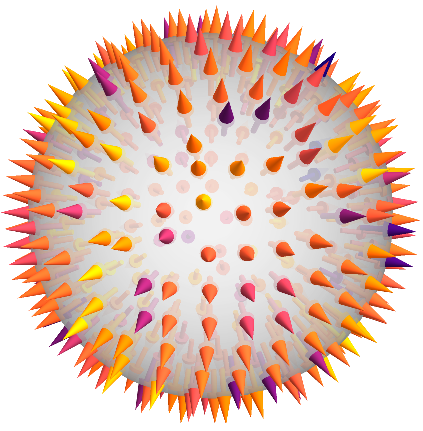
\includegraphics{hedgehog.pdf}
\caption{The hedgehog ansatz, the figure shows the diagram presentation of $\boldsymbol{\pi }$ field, the length of the arrow is proportional to $F( r)$.}
\label{fig:hedgehog}
\end{figure}

Now we try to determine the boundary condition of $F( r)$. We know $SU( 2) \cong S^{3} =\mathbb{R}^{3} \cup \{\infty \}$, we can set $U(| \boldsymbol{x}| \rightarrow \infty )=\mathds{1}$(this means the field becomes vacuum at the infinity physically), then we have
\begin{equation*}
F( \infty ) =0.
\end{equation*}
We can then expand $U_{H}$:
\begin{equation*}
U_{H}( r) =\cos F( r)\mathds{1} +\mathrm{i}\sin F( r)\hat{\boldsymbol{r}} \cdot \boldsymbol{\sigma } ,
\end{equation*}
which means $F$ is actually the azimuthal angle of the group space. At the origin, our field cannot have any `out-pointing' component, due to continuity. Therefore, our boundary condition must impose that $\sin F(0)=0$, which implies
\begin{equation*}
F(0)=n\pi ,\ \ n\in \mathbb{Z} .
\end{equation*}
With these two boundary condition, we can actually calculate the topological charge, i.e. the additional term in the gauge transformation \eqref{eq:gaugeTransformationOfCSAction} of $S_{CS}$:
\begin{equation*}
\mathcal{B} \equiv \operatorname{tr} ((U^{-1} \mathrm{d} U)^{3} )=\frac{1}{2\pi ^{2} r^{2}} F'( r)\sin^{2}( F( r)) ,
\end{equation*}
and the integration gives:
\begin{equation}
\begin{aligned}
B[ U_{H}] & \equiv \frac{1}{24\pi ^{2}} \epsilon _{ijk}\int \mathrm{d}^{3} x\operatorname{tr} ((U^{-1} \mathrm{d} U)^{3} )\\
 & =-\frac{2}{\pi }\int _{0}^{\infty } F'( r)\sin^{2} F\mathrm{d} r\\
 & =\frac{1}{\pi }\left. \left[\frac{1}{2}\sin 2F-F\right]\right| _{r=0}^{r\rightarrow \infty } =n\in \mathbb{Z} .
\end{aligned}
\label{eq:windingNumberOfU}
\end{equation}
Of course, we can also use the geometry method to compute $B$. Note that $S^{3}$ can be parameterized by three angles $( F,\Theta ,\Phi )$, and $B$ is the winding number of the map, which means we just need to pull back the normalized volume element on $S^{3}$ to the real space. The volume form of $S^{3}$ in $\mathbb{R}^{4}$ is given by
\begin{equation*}
\mathrm{d} \Omega =\sin^{2} F\sin\mathrm{\Theta d} F\land \mathrm{d} \Theta \land \mathrm{d} \Phi ,
\end{equation*}
and the integration gives
\begin{equation*}
\int \mathrm{d} \Omega =\int _{0}^{\pi }\sin^{2} F\mathrm{d} F\int _{0}^{\pi }\sin\mathrm{\Theta d} \Theta \int _{0}^{2\pi }\mathrm{d} \Phi =2\pi ^{2} ,
\end{equation*}
i.e. the normalized volume form is
\begin{equation*}
\hat{\mathrm{d} \Omega } =\frac{1}{2\pi ^{2}}\sin^{2} F\sin\mathrm{\Theta d} F\land \mathrm{d} \Theta \land \mathrm{d} \Phi .
\end{equation*}
Then we define the pull back to be:
\begin{equation*}
\left\{\begin{aligned}
F & \rightarrow F( r) \Rightarrow \mathrm{d} F=F'\mathrm{d} r\\
\Theta  & \rightarrow \theta \\
\Phi  & \rightarrow \phi ,
\end{aligned}\right. ,
\end{equation*}
then the integral in real space equals to
\begin{equation*}
\int _{\mathbb{R}^{3}}\tilde{\hat{\mathrm{d} \Omega }} =\frac{1}{2\pi ^{2}}\int _{\infty }^{0} F'\sin^{2} F\mathrm{d} r\int _{0}^{\pi }\sin \theta \mathrm{d}\int _{0}^{2\pi }\mathrm{d} \Phi ,
\end{equation*}
which will also give \eqref{eq:windingNumberOfU}.

\section{Quantization of Winding Number}
Let us consider the manifold $S^{3}$ which we consider as $\mathbb{R}^{3}$ plus a point at infinity. Consider the gauge transform function defined
\begin{equation*}
U(\boldsymbol{x} )=\exp\left(\frac{\mathrm{i} \pi N\boldsymbol{x} \cdot \boldsymbol{\sigma }}{\sqrt{|\boldsymbol{x} |^{2} +R^{2}}}\right)
\end{equation*}
where $\boldsymbol{x}$ is a point in $\mathbb{R}^{3}$, and $\boldsymbol{\sigma }$ represents the Pauli matrices with $R$ an arbitrary length scale. Show the winding number Eq. $5.16$ gives the integer $N$. Why does $N$ need to be an integer here?

\paragraph{Answer}
We can just repeat our calculation in our last calculation again. To throw away $N$, we consider $B[ U_{1} U_{2}]$. Write it down:
\begin{equation*}
B[ U_{1} U_{2}] =\frac{1}{24\pi ^{2}} \epsilon _{ijk}\int \mathrm{d}^{3} x\operatorname{tr} (U_{2}^{\dagger } U_{1}^{\dagger } \partial _{i}( U_{1} U_{2}) \partial _{j} (U_{2}^{\dagger } U_{1}^{\dagger } )\partial _{k}( U_{1} U_{2}) ).
\end{equation*}
where we have used the identity $( U_{1} U_{2})^{\dagger } \equiv U_{2}^{\dagger } U_{1}$.(Noting that $U$ is unitary, we can use $U^{\dagger }$ instead of $U^{-1}$). Expanding the traced part out yields
\begin{equation*}
\begin{aligned}
 & U_{2}^{\dagger } U_{1}^{\dagger }( \partial _{i} U_{1}) U_{2} (\partial _{j} U_{2}^{\dagger } )U_{1}^{\dagger }( \partial _{k} U_{1}) U_{2} & \text{ term } 1\\
+ & U_{2}^{\dagger } U_{1}^{\dagger }( \partial _{i} U_{1}) U_{2} (\partial _{j} U_{2}^{\dagger } )U_{1}^{\dagger }\textcolor[rgb]{0.82,0.01,0.11}{U_{1}( \partial _{k} U_{2})} & \text{ term } 2\\
+ & \cancel{U_{2}^{\dagger }} U_{1}^{\dagger }( \partial _{i} U_{1})\cancel{U_{2} U_{2}^{\dagger }} (\partial _{j} U_{1}^{\dagger } )( \partial _{k} U_{1})\cancel{U_{2}} & B[ U_{1}]\\
+ & U_{2}^{\dagger } U_{1}^{\dagger }( \partial _{i} U_{1}) U_{2} U_{2}^{\dagger } (\partial _{j} U_{1}^{\dagger } )U_{1}( \partial _{k} U_{2}) & \text{ term } 4\\
+ & U_{2}^{\dagger } U_{1}^{\dagger }\textcolor[rgb]{0.82,0.01,0.11}{U_{1}( \partial _{i} U_{2}) (\partial _{j} U_{2}^{\dagger } )U_{1}^{\dagger }( \partial _{k} U_{1}) U_{2}} & \text{ term } 5\\
+ & U_{2}^{\dagger }\cancel{U_{1}^{\dagger } U_{1}}( \partial _{i} U_{2}) (\partial _{j} U_{2}^{\dagger } )\cancel{U_{1}^{\dagger } U_{1}}( \partial _{k} U_{2}) & B[ U_{2}]\\
+ & U_{2}^{\dagger } U_{1}^{\dagger } U_{1}( \partial _{i} U_{2}) U_{2}^{\dagger } (\partial _{j} U_{1}^{\dagger } )( \partial _{k} U_{1}) U_{2} & \text{ term } 7\\
+ & U_{2}^{\dagger } U_{1}^{\dagger } U_{1}( \partial _{i} U_{2}) U_{2}^{\dagger } (\partial _{j} U_{1}^{\dagger } )\textcolor[rgb]{0.82,0.01,0.11}{U_{1}( \partial _{k} U_{2})} . & \text{ term } 8
\end{aligned}
\end{equation*}
Now we can integrate by part, for example, the red term in term 2 \ gives $U_{1}( \partial _{k} U_{2})\rightarrow -( \partial _{k} U_{1}) U_{2}$, which cancels term 1. Similarly, term 7 cancels term 8. Finally, in term 5 we can integrate by parts three times, which cancels term 4. Which means we have the additive property
\begin{equation*}
B[ U_{1} U_{2}] =B[ U_{1}] +B[ U_{2}] .
\end{equation*}
Then we can see
\begin{equation*}
B[ U(\boldsymbol{x})] =B[U_{1}(\boldsymbol{x})^{N} ]=NB[ U_{1}(\boldsymbol{x})] ,
\end{equation*}
where
\begin{equation*}
U_{1} (\boldsymbol{x} )=\exp\left(\frac{\mathrm{i} \pi \boldsymbol{x} \cdot \boldsymbol{\sigma }}{\sqrt{|\boldsymbol{x} |^{2} +R^{2}}}\right) .
\end{equation*}
Then we try to compute $B[ U_{1}]$. Expand first:
\begin{equation*}
U_{1}(\boldsymbol{x}) =\cos\left(\frac{\mathrm{i} \pi | \boldsymbol{x}| }{\sqrt{|\boldsymbol{x} |^{2} +R^{2}}}\right)\mathds{1} +\mathrm{i}\sin\left(\frac{\mathrm{i} \pi | \boldsymbol{x}| }{\sqrt{|\boldsymbol{x} |^{2} +R^{2}}}\right)\boldsymbol{n} \cdot \boldsymbol{\sigma } .
\end{equation*}
Where $\boldsymbol{n} =\boldsymbol{x} /| \boldsymbol{x}| $. We also embed the base space $S^{3}$ into $\mathbb{R}^{4}$ like before, while this time, we can use the coordinate
\begin{equation*}
y^{0} \equiv \cos\left(\frac{\mathrm{i} \pi | \boldsymbol{x}| }{\sqrt{|\boldsymbol{x} |^{2} +R^{2}}}\right) ,\quad \boldsymbol{y} =\sin\left(\frac{\mathrm{i} \pi | \boldsymbol{x}| }{\sqrt{|\boldsymbol{x} |^{2} +R^{2}}}\right)\boldsymbol{n} .
\end{equation*}
Then
\begin{equation*}
U_{1} \equiv y^{0}\mathds{1} +\boldsymbol{y} \cdot \boldsymbol{\sigma } ,
\end{equation*}
with the condition $(y^{0} )^{2} +\boldsymbol{y}^{2} =1$. The winding number clearly doesn't depend on the coordinate, we can use the point $y^{0} =1$, i.e. the north pole to evaluate $B$. Now
\begin{equation*}
\begin{aligned}
\mathcal{B}[ U_{1}] & =\operatorname{tr} ((U_{1}^{-1}\mathrm{d} U_{1} )^{3} )=\operatorname{tr} [(\mathrm{id}\boldsymbol{y} \cdot \boldsymbol{\sigma } )^{3} ]\\
 & =\mathrm{i}^{3} 3!\operatorname{tr}( \sigma _{1} \sigma _{2} \sigma _{3})\mathrm{d} y^{1} \land \mathrm{d} y^{2}\mathrm{\land d} y^{3}\\
 & =12\mathrm{d} y^{1} \land \mathrm{d} y^{2}\mathrm{\land d} y^{3} .
\end{aligned}
\end{equation*}
Then the integration over $\mathbb{R}^{3}$ gives
\begin{equation*}
B[ U_{1}] =\frac{1}{24\pi ^{2}} \times 12\times 2\pi ^{2} =1.
\end{equation*}
Finally, we can see
\begin{equation*}
B[ U(\boldsymbol{x})] =NB[ U_{1}] =N.
\end{equation*}
Besides, at the infinity, we have
\begin{equation*}
U(\boldsymbol{x}\rightarrow \infty )=\exp(\mathrm{i} \pi N\boldsymbol{n} \cdot \boldsymbol{\sigma }) ,
\end{equation*}
which should be independent of $\boldsymbol{n}$(or more physically, $U\rightarrow \mathds{1}$), which means $\sin( N\pi ) =0$, thus $N$ must be an integer. 


\chapter{Short Digression on Quantum Gravity}
\chapter{Defining Topological Quantum Field Theory}

\part{Anyon Basics}

\chapter{Fusion and Structure of Hilbert Space}


\section{Quantum Dimension}
Let $N_{ab}^{c}$ be the fusion multiplicity matrices of a TQFT
\begin{equation*}
a\times b=\sum _{c} N_{ab}^{c} c
\end{equation*}
meaning that $N_{ab}^{c}$ is the number of distinct ways that $a$ and $b$ can fuse to $c$. (In many, or even most, theories of interest all $N$ 's are either 0 or 1 ).



The quantum dimension $\mathsf{d}_{a}$ of a particle $a$ is defined as the largest eigenvalue of the matrix $[ N_{a}]_{b}^{c}$ where this is now thought of as a two dimensional matrix with $a$ fixed and $b,c$ the indices.

Show that
\begin{equation*}
\mathsf{d}_{a}\mathsf{d}_{b} =\sum _{c} N_{ab}^{c}\mathsf{d}_{c} .
\end{equation*}
We will prove this formula algebraically in Chapter 17. However there is a simple and much more physical way to get to the the result: Imagine fusing together $M$ anyons of type $a$ and $M$ anyons of type $b$ where $M$ gets very large and determine the dimension of space that results. Then imagine fusing together $a\times b$ and do this $M$ times and then fuse together all the results.

\paragraph{Answer}
We first consider the fusion of $M$ anyons of type $a$, as the Fig.\ref{fig:fusionOfMAnyonsOfTypea} shows. 
\begin{figure}[h!]
\centering
\tikzset{every picture/.style={line width=0.75pt}} %set default line width to 0.75pt        

\begin{tikzpicture}[x=0.75pt,y=0.75pt,yscale=-1,xscale=1]
%uncomment if require: \path (0,115); %set diagram left start at 0, and has height of 115

%Straight Lines [id:da11955497661468573] 
\draw [color={rgb, 255:red, 74; green, 144; blue, 226 }  ,draw opacity=1 ]   (243,14.64) -- (327.81,112.57) ;
%Straight Lines [id:da6152525920183469] 
\draw [color={rgb, 255:red, 74; green, 144; blue, 226 }  ,draw opacity=1 ]   (271.29,47.31) -- (299.58,14.64) ;
%Straight Lines [id:da819418313740367] 
\draw [color={rgb, 255:red, 74; green, 144; blue, 226 }  ,draw opacity=1 ]   (290.13,69.06) -- (337.26,14.64) ;
%Straight Lines [id:da720895407290538] 
\draw [color={rgb, 255:red, 74; green, 144; blue, 226 }  ,draw opacity=1 ]   (308.97,90.82) -- (374.94,14.64) ;

% Text Node
\draw (248.71,5.06) node [anchor=north west][inner sep=0.75pt]    {$a$};
% Text Node
\draw (285.46,5.06) node [anchor=north west][inner sep=0.75pt]    {$a$};
% Text Node
\draw (267.53,57.33) node [anchor=north west][inner sep=0.75pt]    {$a_{1}$};
% Text Node
\draw (322.21,5.06) node [anchor=north west][inner sep=0.75pt]    {$a$};
% Text Node
\draw (356.28,5.06) node [anchor=north west][inner sep=0.75pt]    {$a$};
% Text Node
\draw (285.08,79.66) node [anchor=north west][inner sep=0.75pt]    {$a_{2}$};
% Text Node
\draw (323.23,96.66) node [anchor=north west][inner sep=0.75pt]    {$\cdots $};
% Text Node
\draw (387.77,5.06) node [anchor=north west][inner sep=0.75pt]    {$\cdots $};
\end{tikzpicture}
\caption{Fusion of $M$ anyons of type $a$.}
\label{fig:fusionOfMAnyonsOfTypea}
\end{figure}
Suppose the final result is $a_{M-1}$, then the dimension of fusing $M$ anyons of type $a$ to get $a_{f}$ is:
\begin{equation*}
\dim( a_{M-1}) =\sum _{a_{1} ,a_{2} \cdots a_{M-2}} N_{aa}^{a_{1}} N_{a_{1} a}^{a_{2}} \cdots N_{a_{M-2} a}^{a_{M-1}} =[( N_{a})^{M-1} ]_{a}^{a_{M-1}} .
\end{equation*}
Similarly, the fusiong of $M$ anyons of type $b$ gives
\begin{equation*}
\dim( b_{M-1}) =[( N_{b})^{M-1} ]_{b}^{b_{M-1}} .
\end{equation*}
Then the fusion of $a_{M-1}$ and $b_{M-1}$ gives
\begin{equation*}
\dim( a_{M-1} \times b_{M-1}) =\sum _{a_{M-1} b_{M-1}} [( N_{b})^{M-1} ]_{b}^{b_{M-1}} [( N_{a})^{M-1} ]_{a}^{a_{M-1}} N_{a_{M-1} b_{M-1}}^{c_{M-1}} .
\end{equation*}
In large $M$ limit, we have
\begin{equation*}
\dim( a_{M-1} \times b_{M-1}) \sim (\mathsf{d}_{b}\mathsf{d}_{a})^{M-1} .
\end{equation*}


However, if we fuse $a,b$ first to give $c$, then fuse $M$ anyons of type $c$, as the Fig.\ref{fig:FusionabFirst} shows, we get
\begin{equation*}
\dim( c_{M-1}) =[(N_{ab}^{c} N_{c} )^{M-1} ]_{c}^{c_{M-1}} N_{ab}^{c} \sim (N_{ab}^{c}\mathsf{d}_{c} )^{M-1} =\dim( a_{M-1} \times b_{M-1}) .
\end{equation*}
\begin{figure}[h!]
\centering
\tikzset{every picture/.style={line width=0.75pt}} %set default line width to 0.75pt        

\begin{tikzpicture}[x=0.75pt,y=0.75pt,yscale=-1,xscale=1]
%uncomment if require: \path (0,137); %set diagram left start at 0, and has height of 137

%Straight Lines [id:da40929728188110026] 
\draw [color={rgb, 255:red, 74; green, 144; blue, 226 }  ,draw opacity=1 ]   (246,33.64) -- (330.81,131.57) ;
%Straight Lines [id:da9953461415866856] 
\draw [color={rgb, 255:red, 74; green, 144; blue, 226 }  ,draw opacity=1 ]   (274.29,66.31) -- (302.58,33.64) ;
%Straight Lines [id:da2994930570192573] 
\draw [color={rgb, 255:red, 74; green, 144; blue, 226 }  ,draw opacity=1 ]   (293.13,88.06) -- (340.26,33.64) ;
%Straight Lines [id:da8153796656269163] 
\draw [color={rgb, 255:red, 74; green, 144; blue, 226 }  ,draw opacity=1 ]   (311.97,109.82) -- (377.94,33.64) ;
%Straight Lines [id:da22124282289903574] 
\draw [color={rgb, 255:red, 208; green, 2; blue, 27 }  ,draw opacity=1 ]   (229.24,14.29) -- (246,33.64) ;
%Straight Lines [id:da6870786384443515] 
\draw [color={rgb, 255:red, 208; green, 2; blue, 27 }  ,draw opacity=1 ]   (262.76,14.29) -- (246,33.64) ;
%Straight Lines [id:da8781455879150906] 
\draw [color={rgb, 255:red, 208; green, 2; blue, 27 }  ,draw opacity=1 ]   (285.81,14.29) -- (302.58,33.64) ;
%Straight Lines [id:da6766518363879819] 
\draw [color={rgb, 255:red, 208; green, 2; blue, 27 }  ,draw opacity=1 ]   (319.34,14.29) -- (302.58,33.64) ;
%Straight Lines [id:da07038864761619235] 
\draw [color={rgb, 255:red, 208; green, 2; blue, 27 }  ,draw opacity=1 ]   (323.49,14.29) -- (340.26,33.64) ;
%Straight Lines [id:da6906279364980574] 
\draw [color={rgb, 255:red, 208; green, 2; blue, 27 }  ,draw opacity=1 ]   (357.02,14.29) -- (340.26,33.64) ;
%Straight Lines [id:da9480406401134733] 
\draw [color={rgb, 255:red, 208; green, 2; blue, 27 }  ,draw opacity=1 ]   (361.18,14.29) -- (377.94,33.64) ;
%Straight Lines [id:da4926866941860706] 
\draw [color={rgb, 255:red, 208; green, 2; blue, 27 }  ,draw opacity=1 ]   (394.7,14.29) -- (377.94,33.64) ;

% Text Node
\draw (236.71,35.03) node [anchor=north west][inner sep=0.75pt]    {$c$};
% Text Node
\draw (299.46,35.03) node [anchor=north west][inner sep=0.75pt]    {$c$};
% Text Node
\draw (270.53,76.33) node [anchor=north west][inner sep=0.75pt]    {$c_{1}$};
% Text Node
\draw (288.08,97.66) node [anchor=north west][inner sep=0.75pt]    {$c_{2}$};
% Text Node
\draw (326.23,115.66) node [anchor=north west][inner sep=0.75pt]    {$\cdots $};
% Text Node
\draw (213,5) node [anchor=north west][inner sep=0.75pt]    {$a$};
% Text Node
\draw (248,2) node [anchor=north west][inner sep=0.75pt]    {$b$};
% Text Node
\draw (274,5) node [anchor=north west][inner sep=0.75pt]    {$a$};
% Text Node
\draw (307,2) node [anchor=north west][inner sep=0.75pt]    {$b$};
% Text Node
\draw (328,5) node [anchor=north west][inner sep=0.75pt]    {$a$};
% Text Node
\draw (346,2) node [anchor=north west][inner sep=0.75pt]    {$b$};
% Text Node
\draw (364,5) node [anchor=north west][inner sep=0.75pt]    {$a$};
% Text Node
\draw (395,2) node [anchor=north west][inner sep=0.75pt]    {$b$};
% Text Node
\draw (336.46,35.03) node [anchor=north west][inner sep=0.75pt]    {$c$};
% Text Node
\draw (373.46,35.03) node [anchor=north west][inner sep=0.75pt]    {$c$};
% Text Node
\draw (417,4) node [anchor=north west][inner sep=0.75pt]    {$\cdots $};
% Text Node
\draw (410,35.03) node [anchor=north west][inner sep=0.75pt]    {$\cdots $};
\end{tikzpicture}
\caption{Fuse $a,b$ first to give $c$, then fuse $M$ anyons of type $c$.}
\label{fig:FusionabFirst}
\end{figure}

So we have
\begin{equation*}
\mathsf{d}_{a}\mathsf{d}_{b} =\sum _{c} N_{ab}^{c}\mathsf{d}_{c} .
\end{equation*}


\section{Fusion and Ground State Degeneracy}
To determine the ground state degeneracy of a 2-manifold in a $2+1$ dimensional TQFT one can cut the manifold into pieces and sew back together. One can think of the open "edges" or connecting tube-ends as each having a label given by one of the particle types (i.e., one of the anyons) of the theory. Really we are labeling each edge with a basis element of a possible Hilbert space. The labels on two tubes that have been connected together must match (label $a$ on one tube fits into label $\bar{a}$ on another tube.) To calculate the ground state degeneracy we must keep track of all possible ways that these assembled tubes could have been labeled. For example, when we assemble a torus as in Fig.\ref{fig:suregeringSphereToTorus}, we must match the quantum number on one open end to the (opposite) quantum number on the opposite open end. The ground state degeneracy is then just the number of different possible labels, or equivalently the number of different particle types.
\begin{figure}[h!]
\centering
\tikzset{every picture/.style={line width=0.75pt}} %set default line width to 0.75pt        

\begin{tikzpicture}[x=0.75pt,y=0.75pt,yscale=-1,xscale=1]
%uncomment if require: \path (0,133); %set diagram left start at 0, and has height of 133

%Shape: Ellipse [id:dp8367832127596704] 
\draw  [color={rgb, 255:red, 74; green, 144; blue, 226 }  ,draw opacity=1 ] (127.97,90.78) .. controls (127.97,69.73) and (145.03,52.67) .. (166.08,52.67) .. controls (187.12,52.67) and (204.18,69.73) .. (204.18,90.78) .. controls (204.18,111.82) and (187.12,128.88) .. (166.08,128.88) .. controls (145.03,128.88) and (127.97,111.82) .. (127.97,90.78) -- cycle ;
%Shape: Ellipse [id:dp3840252547503711] 
\draw  [color={rgb, 255:red, 74; green, 144; blue, 226 }  ,draw opacity=1 ][fill={rgb, 255:red, 200; green, 200; blue, 200 }  ,fill opacity=1 ] (149.22,62.94) .. controls (149.22,61.16) and (151.79,59.72) .. (154.95,59.72) .. controls (158.12,59.72) and (160.69,61.16) .. (160.69,62.94) .. controls (160.69,64.72) and (158.12,66.16) .. (154.95,66.16) .. controls (151.79,66.16) and (149.22,64.72) .. (149.22,62.94) -- cycle ;
%Shape: Ellipse [id:dp6826244717089338] 
\draw  [color={rgb, 255:red, 74; green, 144; blue, 226 }  ,draw opacity=1 ][fill={rgb, 255:red, 200; green, 200; blue, 200 }  ,fill opacity=1 ] (172.22,62.94) .. controls (172.22,61.16) and (174.79,59.72) .. (177.95,59.72) .. controls (181.12,59.72) and (183.69,61.16) .. (183.69,62.94) .. controls (183.69,64.72) and (181.12,66.16) .. (177.95,66.16) .. controls (174.79,66.16) and (172.22,64.72) .. (172.22,62.94) -- cycle ;
%Shape: Arc [id:dp6152757783671656] 
\draw  [draw opacity=0][dash pattern={on 4.5pt off 4.5pt}] (128.02,90.12) .. controls (128.02,90.07) and (128.02,90.02) .. (128.02,89.97) .. controls (128.02,84.41) and (145.03,79.9) .. (166.02,79.9) .. controls (185.99,79.9) and (202.36,83.98) .. (203.9,89.17) -- (166.02,89.97) -- cycle ; \draw  [color={rgb, 255:red, 74; green, 144; blue, 226 }  ,draw opacity=1 ][dash pattern={on 4.5pt off 4.5pt}] (128.02,90.12) .. controls (128.02,90.07) and (128.02,90.02) .. (128.02,89.97) .. controls (128.02,84.41) and (145.03,79.9) .. (166.02,79.9) .. controls (185.99,79.9) and (202.36,83.98) .. (203.9,89.17) ;  
%Shape: Arc [id:dp8238926984639989] 
\draw  [draw opacity=0] (204.13,89.83) .. controls (204.13,89.87) and (204.13,89.92) .. (204.13,89.97) .. controls (204.13,97.15) and (187.07,102.97) .. (166.02,102.97) .. controls (145.76,102.97) and (129.19,97.58) .. (127.97,90.78) -- (166.02,89.97) -- cycle ; \draw  [color={rgb, 255:red, 74; green, 144; blue, 226 }  ,draw opacity=1 ] (204.13,89.83) .. controls (204.13,89.87) and (204.13,89.92) .. (204.13,89.97) .. controls (204.13,97.15) and (187.07,102.97) .. (166.02,102.97) .. controls (145.76,102.97) and (129.19,97.58) .. (127.97,90.78) ;  

%Shape: Arc [id:dp4467037992836296] 
\draw  [draw opacity=0] (301.07,57.36) .. controls (312.85,63.84) and (320.84,76.38) .. (320.84,90.78) .. controls (320.84,111.82) and (303.78,128.88) .. (282.73,128.88) .. controls (261.68,128.88) and (244.62,111.82) .. (244.62,90.78) .. controls (244.62,76.24) and (252.76,63.6) .. (264.73,57.18) -- (282.73,90.78) -- cycle ; \draw  [color={rgb, 255:red, 74; green, 144; blue, 226 }  ,draw opacity=1 ] (301.07,57.36) .. controls (312.85,63.84) and (320.84,76.38) .. (320.84,90.78) .. controls (320.84,111.82) and (303.78,128.88) .. (282.73,128.88) .. controls (261.68,128.88) and (244.62,111.82) .. (244.62,90.78) .. controls (244.62,76.24) and (252.76,63.6) .. (264.73,57.18) ;  
%Shape: Arc [id:dp7205402006021362] 
\draw  [draw opacity=0][dash pattern={on 4.5pt off 4.5pt}] (245.34,90.12) .. controls (245.34,90.07) and (245.34,90.02) .. (245.34,89.97) .. controls (245.34,84.41) and (262.35,79.9) .. (283.34,79.9) .. controls (303.31,79.9) and (319.68,83.98) .. (321.22,89.17) -- (283.34,89.97) -- cycle ; \draw  [color={rgb, 255:red, 74; green, 144; blue, 226 }  ,draw opacity=1 ][dash pattern={on 4.5pt off 4.5pt}] (245.34,90.12) .. controls (245.34,90.07) and (245.34,90.02) .. (245.34,89.97) .. controls (245.34,84.41) and (262.35,79.9) .. (283.34,79.9) .. controls (303.31,79.9) and (319.68,83.98) .. (321.22,89.17) ;  
%Shape: Arc [id:dp43274633674857554] 
\draw  [draw opacity=0] (321.45,89.83) .. controls (321.45,89.87) and (321.45,89.92) .. (321.45,89.97) .. controls (321.45,97.15) and (304.39,102.97) .. (283.34,102.97) .. controls (263.08,102.97) and (246.51,97.58) .. (245.29,90.78) -- (283.34,89.97) -- cycle ; \draw  [color={rgb, 255:red, 74; green, 144; blue, 226 }  ,draw opacity=1 ] (321.45,89.83) .. controls (321.45,89.87) and (321.45,89.92) .. (321.45,89.97) .. controls (321.45,97.15) and (304.39,102.97) .. (283.34,102.97) .. controls (263.08,102.97) and (246.51,97.58) .. (245.29,90.78) ;  
%Shape: Arc [id:dp4118506492611691] 
\draw  [draw opacity=0] (276.39,53.19) .. controls (278.45,52.85) and (280.57,52.67) .. (282.73,52.67) .. controls (285.03,52.67) and (287.28,52.87) .. (289.47,53.26) -- (282.73,90.78) -- cycle ; \draw  [color={rgb, 255:red, 74; green, 144; blue, 226 }  ,draw opacity=1 ] (276.39,53.19) .. controls (278.45,52.85) and (280.57,52.67) .. (282.73,52.67) .. controls (285.03,52.67) and (287.28,52.87) .. (289.47,53.26) ;  
%Curve Lines [id:da688444938326165] 
\draw [color={rgb, 255:red, 74; green, 144; blue, 226 }  ,draw opacity=1 ]   (275.3,17.77) .. controls (247.87,19.49) and (265.59,33.77) .. (266.16,61.49) ;
%Curve Lines [id:da13018309697718644] 
\draw [color={rgb, 255:red, 74; green, 144; blue, 226 }  ,draw opacity=1 ]   (290.44,17.77) .. controls (313.02,19.2) and (303.87,30.63) .. (300.73,62.06) ;
%Curve Lines [id:da4262620194086384] 
\draw [color={rgb, 255:red, 74; green, 144; blue, 226 }  ,draw opacity=1 ]   (275.59,27.77) .. controls (268.73,30.35) and (275.87,41.77) .. (277.59,62.35) ;
%Curve Lines [id:da7292343335631404] 
\draw [color={rgb, 255:red, 74; green, 144; blue, 226 }  ,draw opacity=1 ]   (289.59,27.77) .. controls (296.16,32.06) and (291.3,42.06) .. (288.73,62.35) ;
%Shape: Ellipse [id:dp7735587440966025] 
\draw  [color={rgb, 255:red, 74; green, 144; blue, 226 }  ,draw opacity=1 ][fill={rgb, 255:red, 200; green, 200; blue, 200 }  ,fill opacity=1 ] (275.3,17.77) .. controls (277.08,17.77) and (278.52,20.01) .. (278.52,22.77) .. controls (278.52,25.54) and (277.08,27.77) .. (275.3,27.77) .. controls (273.53,27.77) and (272.09,25.54) .. (272.09,22.77) .. controls (272.09,20.01) and (273.53,17.77) .. (275.3,17.77) -- cycle ;
%Shape: Ellipse [id:dp9340869875314193] 
\draw  [color={rgb, 255:red, 74; green, 144; blue, 226 }  ,draw opacity=1 ][fill={rgb, 255:red, 200; green, 200; blue, 200 }  ,fill opacity=1 ] (290.44,17.77) .. controls (292.22,17.77) and (293.66,20.01) .. (293.67,22.77) .. controls (293.67,25.53) and (292.24,27.77) .. (290.46,27.77) .. controls (288.69,27.78) and (287.24,25.54) .. (287.24,22.78) .. controls (287.23,20.02) and (288.67,17.78) .. (290.44,17.77) -- cycle ;
%Shape: Ellipse [id:dp901311136600087] 
\draw  [color={rgb, 255:red, 74; green, 144; blue, 226 }  ,draw opacity=1 ][dash pattern={on 0.84pt off 2.51pt}] (265.87,64.02) .. controls (265.87,61.79) and (268.43,59.99) .. (271.59,59.99) .. controls (274.74,59.99) and (277.3,61.79) .. (277.3,64.02) .. controls (277.3,66.25) and (274.74,68.05) .. (271.59,68.05) .. controls (268.43,68.05) and (265.87,66.25) .. (265.87,64.02) -- cycle ;
%Shape: Ellipse [id:dp7238920558247142] 
\draw  [color={rgb, 255:red, 74; green, 144; blue, 226 }  ,draw opacity=1 ][dash pattern={on 0.84pt off 2.51pt}] (288.73,63.35) .. controls (288.73,61.12) and (291.29,59.31) .. (294.44,59.31) .. controls (297.6,59.31) and (300.16,61.12) .. (300.16,63.35) .. controls (300.16,65.57) and (297.6,67.38) .. (294.44,67.38) .. controls (291.29,67.38) and (288.73,65.57) .. (288.73,63.35) -- cycle ;
%Curve Lines [id:da26315356637230347] 
\draw [color={rgb, 255:red, 74; green, 144; blue, 226 }  ,draw opacity=1 ] [dash pattern={on 0.84pt off 2.51pt}]  (264.73,57.18) .. controls (270.09,54.63) and (272.95,53.77) .. (276.39,53.19) ;
%Curve Lines [id:da6684748312393574] 
\draw [color={rgb, 255:red, 74; green, 144; blue, 226 }  ,draw opacity=1 ] [dash pattern={on 0.84pt off 2.51pt}]  (289.47,53.26) .. controls (293.81,54.63) and (298.09,56.34) .. (301.07,57.36) ;

%Shape: Arc [id:dp17855570452094005] 
\draw  [draw opacity=0] (418.34,57.36) .. controls (430.12,63.84) and (438.11,76.38) .. (438.11,90.78) .. controls (438.11,111.82) and (421.05,128.88) .. (400,128.88) .. controls (378.95,128.88) and (361.89,111.82) .. (361.89,90.78) .. controls (361.89,76.24) and (370.03,63.6) .. (382,57.18) -- (400,90.78) -- cycle ; \draw  [color={rgb, 255:red, 74; green, 144; blue, 226 }  ,draw opacity=1 ] (418.34,57.36) .. controls (430.12,63.84) and (438.11,76.38) .. (438.11,90.78) .. controls (438.11,111.82) and (421.05,128.88) .. (400,128.88) .. controls (378.95,128.88) and (361.89,111.82) .. (361.89,90.78) .. controls (361.89,76.24) and (370.03,63.6) .. (382,57.18) ;  
%Shape: Arc [id:dp28210159024338144] 
\draw  [draw opacity=0][dash pattern={on 4.5pt off 4.5pt}] (362.61,90.12) .. controls (362.61,90.07) and (362.61,90.02) .. (362.61,89.97) .. controls (362.61,84.41) and (379.62,79.9) .. (400.61,79.9) .. controls (420.58,79.9) and (436.95,83.98) .. (438.49,89.17) -- (400.61,89.97) -- cycle ; \draw  [color={rgb, 255:red, 74; green, 144; blue, 226 }  ,draw opacity=1 ][dash pattern={on 4.5pt off 4.5pt}] (362.61,90.12) .. controls (362.61,90.07) and (362.61,90.02) .. (362.61,89.97) .. controls (362.61,84.41) and (379.62,79.9) .. (400.61,79.9) .. controls (420.58,79.9) and (436.95,83.98) .. (438.49,89.17) ;  
%Shape: Arc [id:dp22378592043269396] 
\draw  [draw opacity=0] (438.72,89.83) .. controls (438.72,89.87) and (438.72,89.92) .. (438.72,89.97) .. controls (438.72,97.15) and (421.66,102.97) .. (400.61,102.97) .. controls (380.35,102.97) and (363.78,97.58) .. (362.56,90.78) -- (400.61,89.97) -- cycle ; \draw  [color={rgb, 255:red, 74; green, 144; blue, 226 }  ,draw opacity=1 ] (438.72,89.83) .. controls (438.72,89.87) and (438.72,89.92) .. (438.72,89.97) .. controls (438.72,97.15) and (421.66,102.97) .. (400.61,102.97) .. controls (380.35,102.97) and (363.78,97.58) .. (362.56,90.78) ;  
%Shape: Arc [id:dp5673270077707613] 
\draw  [draw opacity=0] (393.66,53.19) .. controls (395.72,52.85) and (397.84,52.67) .. (400,52.67) .. controls (402.3,52.67) and (404.55,52.87) .. (406.74,53.26) -- (400,90.78) -- cycle ; \draw  [color={rgb, 255:red, 74; green, 144; blue, 226 }  ,draw opacity=1 ] (393.66,53.19) .. controls (395.72,52.85) and (397.84,52.67) .. (400,52.67) .. controls (402.3,52.67) and (404.55,52.87) .. (406.74,53.26) ;  
%Curve Lines [id:da6964200857303049] 
\draw [color={rgb, 255:red, 74; green, 144; blue, 226 }  ,draw opacity=1 ]   (407.71,17.77) .. controls (357.17,15.38) and (382.86,33.77) .. (383.43,61.49) ;
%Curve Lines [id:da8297872501866517] 
\draw [color={rgb, 255:red, 74; green, 144; blue, 226 }  ,draw opacity=1 ]   (407.71,17.77) .. controls (430.29,19.2) and (421.14,30.63) .. (418,62.06) ;
%Curve Lines [id:da15268769916065472] 
\draw [color={rgb, 255:red, 74; green, 144; blue, 226 }  ,draw opacity=1 ]   (406.86,27.77) .. controls (378.37,21.78) and (393.14,41.77) .. (394.86,62.35) ;
%Curve Lines [id:da8643191076081997] 
\draw [color={rgb, 255:red, 74; green, 144; blue, 226 }  ,draw opacity=1 ]   (406.86,27.77) .. controls (413.14,29.78) and (408.57,42.06) .. (406,62.35) ;
%Shape: Ellipse [id:dp1420571645997517] 
\draw  [color={rgb, 255:red, 74; green, 144; blue, 226 }  ,draw opacity=1 ][dash pattern={on 0.84pt off 2.51pt}] (383.14,64.02) .. controls (383.14,61.79) and (385.7,59.99) .. (388.86,59.99) .. controls (392.01,59.99) and (394.57,61.79) .. (394.57,64.02) .. controls (394.57,66.25) and (392.01,68.05) .. (388.86,68.05) .. controls (385.7,68.05) and (383.14,66.25) .. (383.14,64.02) -- cycle ;
%Shape: Ellipse [id:dp2225371309933939] 
\draw  [color={rgb, 255:red, 74; green, 144; blue, 226 }  ,draw opacity=1 ][dash pattern={on 0.84pt off 2.51pt}] (406,63.35) .. controls (406,61.12) and (408.56,59.31) .. (411.71,59.31) .. controls (414.87,59.31) and (417.43,61.12) .. (417.43,63.35) .. controls (417.43,65.57) and (414.87,67.38) .. (411.71,67.38) .. controls (408.56,67.38) and (406,65.57) .. (406,63.35) -- cycle ;
%Curve Lines [id:da10198974922585369] 
\draw [color={rgb, 255:red, 74; green, 144; blue, 226 }  ,draw opacity=1 ] [dash pattern={on 0.84pt off 2.51pt}]  (382,57.18) .. controls (387.36,54.63) and (390.22,53.77) .. (393.66,53.19) ;
%Curve Lines [id:da3742738353108166] 
\draw [color={rgb, 255:red, 74; green, 144; blue, 226 }  ,draw opacity=1 ] [dash pattern={on 0.84pt off 2.51pt}]  (406.74,53.26) .. controls (411.08,54.63) and (415.36,56.34) .. (418.34,57.36) ;

%Shape: Ellipse [id:dp45593126164338327] 
\draw  [color={rgb, 255:red, 74; green, 144; blue, 226 }  ,draw opacity=1 ] (479.19,92.12) .. controls (479.19,83.52) and (491.39,76.55) .. (506.44,76.55) .. controls (521.5,76.55) and (533.7,83.52) .. (533.7,92.12) .. controls (533.7,100.72) and (521.5,107.7) .. (506.44,107.7) .. controls (491.39,107.7) and (479.19,100.72) .. (479.19,92.12) -- cycle ;
%Shape: Arc [id:dp27723580182468344] 
\draw  [draw opacity=0] (492.5,94.55) .. controls (492.49,94.47) and (492.49,94.39) .. (492.49,94.32) .. controls (492.49,89.4) and (498.67,85.42) .. (506.3,85.42) .. controls (513.32,85.42) and (519.12,88.8) .. (519.99,93.17) -- (506.3,94.32) -- cycle ; \draw  [color={rgb, 255:red, 74; green, 144; blue, 226 }  ,draw opacity=1 ] (492.5,94.55) .. controls (492.49,94.47) and (492.49,94.39) .. (492.49,94.32) .. controls (492.49,89.4) and (498.67,85.42) .. (506.3,85.42) .. controls (513.32,85.42) and (519.12,88.8) .. (519.99,93.17) ;  
%Shape: Arc [id:dp9068851295860665] 
\draw  [draw opacity=0] (522.14,89.36) .. controls (522.15,89.5) and (522.16,89.64) .. (522.16,89.78) .. controls (522.16,94.46) and (515.12,98.26) .. (506.44,98.26) .. controls (498.66,98.26) and (492.2,95.21) .. (490.95,91.2) -- (506.44,89.78) -- cycle ; \draw  [color={rgb, 255:red, 74; green, 144; blue, 226 }  ,draw opacity=1 ] (522.14,89.36) .. controls (522.15,89.5) and (522.16,89.64) .. (522.16,89.78) .. controls (522.16,94.46) and (515.12,98.26) .. (506.44,98.26) .. controls (498.66,98.26) and (492.2,95.21) .. (490.95,91.2) ;  


% Text Node
\draw (211.4,82.11) node [anchor=north west][inner sep=0.75pt]    {$\Rightarrow $};
% Text Node
\draw (328.67,82.11) node [anchor=north west][inner sep=0.75pt]    {$\Rightarrow $};
% Text Node
\draw (445.94,82.11) node [anchor=north west][inner sep=0.75pt]    {$\Rightarrow $};
% Text Node
\draw (174.22,65.61) node [anchor=north west][inner sep=0.75pt]    {$a$};
% Text Node
\draw (147.89,65.61) node [anchor=north west][inner sep=0.75pt]    {$\bar{a}$};
% Text Node
\draw (286.87,2.61) node [anchor=north west][inner sep=0.75pt]    {$a$};
% Text Node
\draw (268.54,2.61) node [anchor=north west][inner sep=0.75pt]    {$\bar{a}$};
\end{tikzpicture}
\caption{Surgering the twice punctured sphere into a torus. This is the gluing axiom in action. Note that we are implicitly assuming the system is trivial in the ``time” direction, which we assume to form a circle $S_{\text{time}}^{1}$.}
\label{fig:suregeringSphereToTorus}
\end{figure}

For more complicated 2-d manifolds, we can decompose the manifold into so-called pants diagrams that look like Fig.\ref{fig:pairOfPants}. When we sew together pants diagrams, we should include a factor of the fusions multiplicity $N_{ab}^{c}$ for each pants which has its three tube edges labeled with $a,b$ and $\bar{c}$.
\begin{figure}[h!]
\centering
\tikzset{every picture/.style={line width=0.75pt}} %set default line width to 0.75pt        

\begin{tikzpicture}[x=0.75pt,y=0.75pt,yscale=-1,xscale=1]
%uncomment if require: \path (0,109); %set diagram left start at 0, and has height of 109

%Shape: Arc [id:dp05657397073367365] 
\draw  [draw opacity=0][dash pattern={on 4.5pt off 4.5pt}] (215.19,65.11) .. controls (215.18,65.06) and (215.18,65.01) .. (215.18,64.96) .. controls (215.18,59.4) and (232.2,54.89) .. (253.18,54.89) .. controls (273.15,54.89) and (289.53,58.97) .. (291.07,64.16) -- (253.18,64.96) -- cycle ; \draw  [color={rgb, 255:red, 74; green, 144; blue, 226 }  ,draw opacity=1 ][dash pattern={on 4.5pt off 4.5pt}] (215.19,65.11) .. controls (215.18,65.06) and (215.18,65.01) .. (215.18,64.96) .. controls (215.18,59.4) and (232.2,54.89) .. (253.18,54.89) .. controls (273.15,54.89) and (289.53,58.97) .. (291.07,64.16) ;  
%Shape: Ellipse [id:dp11579635984986858] 
\draw  [color={rgb, 255:red, 74; green, 144; blue, 226 }  ,draw opacity=1 ] (214.97,64.6) .. controls (214.97,43.55) and (232.03,26.49) .. (253.08,26.49) .. controls (274.12,26.49) and (291.18,43.55) .. (291.18,64.6) .. controls (291.18,85.64) and (274.12,102.7) .. (253.08,102.7) .. controls (232.03,102.7) and (214.97,85.64) .. (214.97,64.6) -- cycle ;
%Shape: Arc [id:dp9816205265344173] 
\draw  [draw opacity=0] (291.3,64.82) .. controls (291.3,64.87) and (291.3,64.92) .. (291.3,64.96) .. controls (291.3,72.14) and (274.24,77.96) .. (253.18,77.96) .. controls (232.92,77.96) and (216.35,72.57) .. (215.14,65.77) -- (253.18,64.96) -- cycle ; \draw  [color={rgb, 255:red, 74; green, 144; blue, 226 }  ,draw opacity=1 ] (291.3,64.82) .. controls (291.3,64.87) and (291.3,64.92) .. (291.3,64.96) .. controls (291.3,72.14) and (274.24,77.96) .. (253.18,77.96) .. controls (232.92,77.96) and (216.35,72.57) .. (215.14,65.77) ;  
%Shape: Ellipse [id:dp6759124833295995] 
\draw  [color={rgb, 255:red, 74; green, 144; blue, 226 }  ,draw opacity=1 ][fill={rgb, 255:red, 200; green, 200; blue, 200 }  ,fill opacity=1 ] (230.33,41.65) .. controls (229.65,40.01) and (231.45,37.69) .. (234.37,36.46) .. controls (237.29,35.24) and (240.22,35.57) .. (240.9,37.21) .. controls (241.59,38.84) and (239.78,41.17) .. (236.87,42.39) .. controls (233.95,43.62) and (231.02,43.29) .. (230.33,41.65) -- cycle ;
%Shape: Ellipse [id:dp26656071826027805] 
\draw  [color={rgb, 255:red, 74; green, 144; blue, 226 }  ,draw opacity=1 ][fill={rgb, 255:red, 200; green, 200; blue, 200 }  ,fill opacity=1 ] (248.22,32.97) .. controls (248.16,31.2) and (250.67,29.66) .. (253.83,29.55) .. controls (257,29.43) and (259.62,30.78) .. (259.68,32.55) .. controls (259.75,34.33) and (257.23,35.86) .. (254.07,35.98) .. controls (250.91,36.09) and (248.29,34.75) .. (248.22,32.97) -- cycle ;
%Shape: Ellipse [id:dp4548290894023457] 
\draw  [color={rgb, 255:red, 74; green, 144; blue, 226 }  ,draw opacity=1 ][fill={rgb, 255:red, 200; green, 200; blue, 200 }  ,fill opacity=1 ] (266.22,36.83) .. controls (266.82,35.16) and (269.72,34.67) .. (272.7,35.73) .. controls (275.68,36.8) and (277.62,39.02) .. (277.02,40.7) .. controls (276.42,42.37) and (273.52,42.86) .. (270.53,41.79) .. controls (267.55,40.72) and (265.62,38.5) .. (266.22,36.83) -- cycle ;
%Curve Lines [id:da739129157041372] 
\draw [color={rgb, 255:red, 74; green, 144; blue, 226 }  ,draw opacity=1 ]   (345.99,84.21) .. controls (364.37,56.38) and (367.37,44.54) .. (377.99,28.21) ;
%Curve Lines [id:da8017147020708633] 
\draw [color={rgb, 255:red, 74; green, 144; blue, 226 }  ,draw opacity=1 ]   (446.04,83.88) .. controls (435.7,61.21) and (428.04,44.54) .. (420.66,28.54) ;
%Curve Lines [id:da5740408386448019] 
\draw [color={rgb, 255:red, 74; green, 144; blue, 226 }  ,draw opacity=1 ]   (378.37,84.21) .. controls (389.7,57.54) and (402.15,59.21) .. (411.81,83.88) ;
%Shape: Ellipse [id:dp32146447376371046] 
\draw  [color={rgb, 255:red, 74; green, 144; blue, 226 }  ,draw opacity=1 ][fill={rgb, 255:red, 200; green, 200; blue, 200 }  ,fill opacity=1 ] (378.18,28.54) .. controls (378.18,25.45) and (387.69,22.94) .. (399.42,22.94) .. controls (411.15,22.94) and (420.66,25.45) .. (420.66,28.54) .. controls (420.66,31.63) and (411.15,34.14) .. (399.42,34.14) .. controls (387.69,34.14) and (378.18,31.63) .. (378.18,28.54) -- cycle ;
%Shape: Ellipse [id:dp3365369220585279] 
\draw  [color={rgb, 255:red, 74; green, 144; blue, 226 }  ,draw opacity=1 ][fill={rgb, 255:red, 200; green, 200; blue, 200 }  ,fill opacity=1 ] (345.99,84.21) .. controls (345.99,82.16) and (353.24,80.49) .. (362.18,80.49) .. controls (371.12,80.49) and (378.37,82.16) .. (378.37,84.21) .. controls (378.37,86.26) and (371.12,87.93) .. (362.18,87.93) .. controls (353.24,87.93) and (345.99,86.26) .. (345.99,84.21) -- cycle ;
%Shape: Ellipse [id:dp6352897662304982] 
\draw  [color={rgb, 255:red, 74; green, 144; blue, 226 }  ,draw opacity=1 ][fill={rgb, 255:red, 200; green, 200; blue, 200 }  ,fill opacity=1 ] (411.81,83.88) .. controls (411.81,81.82) and (419.47,80.16) .. (428.92,80.16) .. controls (438.38,80.16) and (446.04,81.82) .. (446.04,83.88) .. controls (446.04,85.93) and (438.38,87.59) .. (428.92,87.59) .. controls (419.47,87.59) and (411.81,85.93) .. (411.81,83.88) -- cycle ;

% Text Node
\draw (224.66,17.29) node [anchor=north west][inner sep=0.75pt]    {$a$};
% Text Node
\draw (249.33,10.29) node [anchor=north west][inner sep=0.75pt]    {$b$};
% Text Node
\draw (275.99,17.95) node [anchor=north west][inner sep=0.75pt]    {$c$};
% Text Node
\draw (395.66,4.29) node [anchor=north west][inner sep=0.75pt]    {$a$};
% Text Node
\draw (356.33,88.72) node [anchor=north west][inner sep=0.75pt]    {$b$};
% Text Node
\draw (429.92,88.72) node [anchor=north west][inner sep=0.75pt]    {$c$};
\end{tikzpicture}
\caption{A three-times punctured sphere is known as a ``pair of pants”.}
\label{fig:pairOfPants}
\end{figure}


\begin{enumerate}
\item Write a general formula for the ground state degeneracy of an $M$-handled torus in terms of the $N$ matrices.
\item For the Fibonacci anyon model, find the ground state degeneracy of a 4-handled torus.
\item Show that in the limit of large number of handles $M$ the ground state degeneracy scales as $\sim \mathcal{D}^{2M}$ where $\mathcal{D}^{2} =\sum _{a}\mathrm{\mathsf{d}}_{a}^{2}$.
\end{enumerate}

\paragraph{Answer}



\section{Consistency of Fusion Rules}
Show by using commutativity and associativity of fusion along with identity \eqref{eq:timeReversalPropertyOfN}
\begin{equation}
N_{ab}^{c} =N_{\bar{a}\bar{b}}^{\bar{c}} ,
\label{eq:timeReversalPropertyOfN}
\end{equation}
that no anyon theory can have a particle $a$ such that $a\times a=a$ meaning $a$ fuses to $a$ to form only $a$ and nothing else.

\paragraph{Answer}
Suppose there is a theory that $a\times a=a$ and $a\neq I$, then consider the process of fusing $a,a$ and $\bar{a}$. We can simplicity, we can set the fusion rule between $a,\bar{a}$ is
\begin{equation}
a\times \bar{a} =I+c_{1} +\cdots +c_{n} .
\label{eq:fusionChannelOfaabar}
\end{equation}

As the Fig.\ref{fig:fusionOfThreeAnyons} shows, if we fuse $a\times a=a$ first, then fuse $a\times \bar{a}$, we will get $I+c_{1} +\cdots +c_{n}$ finally. However, if we change the order of fusion, fuse $a\times \bar{a}$ first and get $I+c_{1} +\cdots +c_{n}$, then fuse $a$, we will get 
\begin{equation*}
a\times \bar{a} =a+a\times c_{1} +\cdots +a\times c_{n} .
\end{equation*}
\begin{figure}[h!]
\centering
\tikzset{every picture/.style={line width=0.75pt}} %set default line width to 0.75pt        

\begin{tikzpicture}[x=0.75pt,y=0.75pt,yscale=-1,xscale=1]
%uncomment if require: \path (0,100); %set diagram left start at 0, and has height of 100

%Straight Lines [id:da8590660242956558] 
\draw [color={rgb, 255:red, 74; green, 144; blue, 226 }  ,draw opacity=1 ]   (121,6) -- (211,96) ;
%Straight Lines [id:da4918681534713645] 
\draw [color={rgb, 255:red, 74; green, 144; blue, 226 }  ,draw opacity=1 ]   (151,36) -- (181,6) ;
%Straight Lines [id:da5778336776064139] 
\draw [color={rgb, 255:red, 74; green, 144; blue, 226 }  ,draw opacity=1 ]   (181,66) -- (241,6) ;

%Straight Lines [id:da5712783429115829] 
\draw [color={rgb, 255:red, 74; green, 144; blue, 226 }  ,draw opacity=1 ]   (338,6) -- (428,96) ;
%Straight Lines [id:da00547547016614347] 
\draw [color={rgb, 255:red, 74; green, 144; blue, 226 }  ,draw opacity=1 ]   (428,36) -- (398,6) ;
%Straight Lines [id:da2923856794370401] 
\draw [color={rgb, 255:red, 74; green, 144; blue, 226 }  ,draw opacity=1 ]   (398,66) -- (458,6) ;

% Text Node
\draw (289,40) node [anchor=north west][inner sep=0.75pt]    {$=$};
% Text Node
\draw (132,0) node [anchor=north west][inner sep=0.75pt]    {$a$};
% Text Node
\draw (189,0) node [anchor=north west][inner sep=0.75pt]    {$a$};
% Text Node
\draw (249,0) node [anchor=north west][inner sep=0.75pt]    {$\bar{a}$};
% Text Node
\draw (149,50) node [anchor=north west][inner sep=0.75pt]    {$a$};
% Text Node
\draw (219,80) node [anchor=north west][inner sep=0.75pt]    {$I+c_{1} +\cdots +c_{n}$};
% Text Node
\draw (349,0) node [anchor=north west][inner sep=0.75pt]    {$a$};
% Text Node
\draw (409,0) node [anchor=north west][inner sep=0.75pt]    {$a$};
% Text Node
\draw (466,0) node [anchor=north west][inner sep=0.75pt]    {$\bar{a}$};
% Text Node
\draw (426,40) node [anchor=north west][inner sep=0.75pt]    {$I+c_{1} +\cdots +c_{n}$};
% Text Node
\draw (436,80) node [anchor=north west][inner sep=0.75pt]    {$a+a\times c_{1} +\cdots +a\times c_{n}$};


\end{tikzpicture}
\caption{The fusion of $a,a,\bar{a}$.}
\label{fig:fusionOfThreeAnyons}
\end{figure}

In order to get the same result, we know that $\{a,a\times c_{1} ,\cdots ,a\times c_{n}\}$ must be a permutation of $\{I,c_{1} ,\cdots ,c_{n}\}$, which means $a\times c_{i}$ \textbf{cannot have multiple fusion channels} because each fusion channel have at least one result. Furthermore, in first case, we have $I$ in the final result, so $\exists i$, s.t. $c_{i} =\bar{a}$. Now the rule that $a\times c_{i}$ cannot have multiple fusion channel contradicts with \eqref{eq:fusionChannelOfaabar}, so no anyon theory can have a particle $a$ such that $a\times a=a$.


\chapter{Change of Basis and $F$-Matrices}


\section{$F$\textbf{-gauge choice}}

\begin{enumerate}
\item Explain why in the Fibonacci theory, $[F_{\tau }^{\tau \tau \tau } ]_{\tau \tau }$ is gauge independent but $[F_{\tau }^{\tau \tau \tau } ]_{I\tau }$ is gauge dependent.
\item Explain why in the Ising theory is $[F_{\sigma }^{\psi \sigma \psi } ]_{\sigma \sigma }$ is gauge independent, but $[F_{\psi }^{\sigma \psi \sigma } ]_{\sigma \sigma }$ is gauge dependent.
\end{enumerate}

\paragraph{Answer}
(a) In Fibonacci theory, consider the process $\tau ,\tau ,\tau $ fuse to $\tau $. We have:
\begin{equation*}
\begin{pmatrix}
|0\rangle \\
|1\rangle 
\end{pmatrix} =\begin{pmatrix}
[F_{\tau }^{\tau \tau \tau } ]_{II} & [F_{\tau }^{\tau \tau \tau } ]_{I\tau }\\
[F_{\tau }^{\tau \tau \tau } ]_{\tau I} & [F_{\tau }^{\tau \tau \tau } ]_{\tau \tau }
\end{pmatrix}\begin{pmatrix}
|0'\rangle \\
|1'\rangle 
\end{pmatrix} ,
\end{equation*}
where
\begin{equation*}
\tikzset{every picture/.style={line width=0.75pt}} %set default line width to 0.75pt        
\begin{tikzpicture}[x=0.75pt,y=0.75pt,yscale=-1,xscale=1, baseline=(XXXX.south) ]
\path (0,76);\path (92.9889907836914,0);\draw    ($(current bounding box.center)+(0,0.3em)$) node [anchor=south] (XXXX) {};
%Straight Lines [id:da6679856576688559] 
\draw [color={rgb, 255:red, 74; green, 144; blue, 226 }  ,draw opacity=1 ]   (1.56,14.56) -- (21,34) ;
%Straight Lines [id:da14116196892650712] 
\draw [color={rgb, 255:red, 74; green, 144; blue, 226 }  ,draw opacity=1 ]   (21,34) -- (41,14) ;
%Straight Lines [id:da8326498689328212] 
\draw [color={rgb, 255:red, 74; green, 144; blue, 226 }  ,draw opacity=1 ] [dash pattern={on 0.84pt off 2.51pt}]  (41,54) -- (21,34) ;
%Straight Lines [id:da7982058810830115] 
\draw [color={rgb, 255:red, 74; green, 144; blue, 226 }  ,draw opacity=1 ]   (81,14) -- (21,74) ;
% Text Node
\draw (2,-3.5) node [anchor=north west][inner sep=0.75pt]    {$\tau $};
% Text Node
\draw (42,-3.5) node [anchor=north west][inner sep=0.75pt]    {$\tau $};
% Text Node
\draw (82,-3.5) node [anchor=north west][inner sep=0.75pt]    {$\tau $};
% Text Node
\draw (9,56.5) node [anchor=north west][inner sep=0.75pt]    {$\tau $};
% Text Node
\draw (33,25.5) node [anchor=north west][inner sep=0.75pt]    {$I$};
\end{tikzpicture}
=|0\rangle ,\quad \tikzset{every picture/.style={line width=0.75pt}} %set default line width to 0.75pt        
\begin{tikzpicture}[x=0.75pt,y=0.75pt,yscale=-1,xscale=1, baseline=(XXXX.south) ]
\path (0,76);\path (92.9889907836914,0);\draw    ($(current bounding box.center)+(0,0.3em)$) node [anchor=south] (XXXX) {};
%Straight Lines [id:da23482911055376698] 
\draw [color={rgb, 255:red, 74; green, 144; blue, 226 }  ,draw opacity=1 ]   (2.55,13.54) -- (41.99,52.98) ;
%Straight Lines [id:da5187919992908567] 
\draw [color={rgb, 255:red, 74; green, 144; blue, 226 }  ,draw opacity=1 ]   (21.99,32.98) -- (41.99,12.98) ;
%Straight Lines [id:da6132340599706072] 
\draw [color={rgb, 255:red, 74; green, 144; blue, 226 }  ,draw opacity=1 ]   (81.99,12.98) -- (21.99,72.98) ;
% Text Node
\draw (2.99,-4.52) node [anchor=north west][inner sep=0.75pt]    {$\tau $};
% Text Node
\draw (42.99,-4.52) node [anchor=north west][inner sep=0.75pt]    {$\tau $};
% Text Node
\draw (82.99,-4.52) node [anchor=north west][inner sep=0.75pt]    {$\tau $};
% Text Node
\draw (9.99,55.48) node [anchor=north west][inner sep=0.75pt]    {$\tau $};
% Text Node
\draw (33.99,24.48) node [anchor=north west][inner sep=0.75pt]    {$\tau $};
\end{tikzpicture}
=|1\rangle .
\end{equation*}
Now we consider a gauge transformation on the vertices. According to the transformation rule of $F$, if the on one vertex, the gauge transformation is given by:
\begin{equation*}
\tikzset{every picture/.style={line width=0.75pt}} %set default line width to 0.75pt        
\begin{tikzpicture}[x=0.75pt,y=0.75pt,yscale=-1,xscale=1, baseline=(XXXX.south) ]
\path (0,50);\path (43.98124313354492,0);\draw    ($(current bounding box.center)+(0,0.3em)$) node [anchor=south] (XXXX) {};
%Straight Lines [id:da6721611237810059] 
\draw [color={rgb, 255:red, 74; green, 144; blue, 226 }  ,draw opacity=1 ]   (2,8) -- (22,28) ;
%Straight Lines [id:da27101694568404877] 
\draw [color={rgb, 255:red, 74; green, 144; blue, 226 }  ,draw opacity=1 ]   (22,28) -- (42,8) ;
%Straight Lines [id:da24019406696757506] 
\draw [color={rgb, 255:red, 74; green, 144; blue, 226 }  ,draw opacity=1 ]   (22,48) -- (22,28) ;
% Text Node
\draw (6,0) node [anchor=north west][inner sep=0.75pt]    {$a$};
% Text Node
\draw (26.99,-3) node [anchor=north west][inner sep=0.75pt]    {$b$};
% Text Node
\draw (24,29.5) node [anchor=north west][inner sep=0.75pt]    {$c$};
\end{tikzpicture}
=u_{c}^{ab}\tikzset{every picture/.style={line width=0.75pt}} %set default line width to 0.75pt        
\begin{tikzpicture}[x=0.75pt,y=0.75pt,yscale=-1,xscale=1, baseline=(XXXX.south) ]
\path (0,50);\path (43.98124313354492,0);\draw    ($(current bounding box.center)+(0,0.3em)$) node [anchor=south] (XXXX) {};
%Straight Lines [id:da5541944561024958] 
\draw [color={rgb, 255:red, 74; green, 144; blue, 226 }  ,draw opacity=1 ]   (2,8) -- (22,28) ;
%Straight Lines [id:da395643263838791] 
\draw [color={rgb, 255:red, 74; green, 144; blue, 226 }  ,draw opacity=1 ]   (22,28) -- (42,8) ;
%Straight Lines [id:da8544980505411282] 
\draw [color={rgb, 255:red, 74; green, 144; blue, 226 }  ,draw opacity=1 ]   (22,48) -- (22,28) ;
% Text Node
\draw (6,0) node [anchor=north west][inner sep=0.75pt]    {$a$};
% Text Node
\draw (26.99,-3) node [anchor=north west][inner sep=0.75pt]    {$b$};
% Text Node
\draw (24,29.5) node [anchor=north west][inner sep=0.75pt]    {$c$};
% Text Node
\draw (14.97,8.5) node [anchor=north west][inner sep=0.75pt]  [color={rgb, 255:red, 74; green, 144; blue, 226 }  ,opacity=1 ]  {$\widetilde{\ \ \ }$};
\end{tikzpicture}
,
\end{equation*}
then
\begin{equation*}
[\tilde{F}_{e}^{abc} ]_{df} =\frac{u_{e}^{af} u_{f}^{bc}}{u_{d}^{ab} u_{e}^{dc}} [F_{e}^{abc} ]_{df} .
\end{equation*}
Also note that if one of the upper legs is the identity, we typically do not allow a gauge transform of this type of vertex, i.e.
\begin{equation*}
u_{\tau }^{I\tau } =1.
\end{equation*}
Then
\begin{equation*}
[\tilde{F}_{\tau }^{\tau \tau \tau } ]_{\tau \tau } =\frac{u_{\tau }^{\tau \tau } u_{\tau }^{\tau \tau }}{u_{\tau }^{\tau \tau } u_{\tau }^{\tau \tau }} [F_{\tau }^{\tau \tau \tau } ]_{\tau \tau } =[F_{\tau }^{\tau \tau \tau } ]_{\tau \tau } ,
\end{equation*}
which means $[F_{\tau }^{\tau \tau \tau } ]_{\tau \tau }$ is gauge independent. But for
\begin{equation*}
[\tilde{F}_{\tau }^{\tau \tau \tau } ]_{I\tau } =\frac{u_{\tau }^{\tau \tau } u_{\tau }^{\tau \tau }}{u_{I}^{\tau \tau } u_{\tau }^{\tau \tau }} [F_{\tau }^{\tau \tau \tau } ]_{I\tau } =u_{\tau }^{\tau \tau } [F_{\tau }^{\tau \tau \tau } ]_{I\tau } ,
\end{equation*}
which means $[F_{\tau }^{\tau \tau \tau } ]_{I\tau }$ is gauge dependent. 



(b) For Ising, the case is the same:
\begin{equation*}
[\tilde{F}_{\sigma }^{\psi \sigma \psi } ]_{\sigma \sigma } =\frac{u_{\sigma }^{\psi \sigma } u_{\sigma }^{\sigma \psi }}{u_{\sigma }^{\psi \sigma } u_{\sigma }^{\sigma \psi }} [F_{\sigma }^{\psi \sigma \psi } ]_{\sigma \sigma } =[F_{\sigma }^{\psi \sigma \psi } ]_{\sigma \sigma } ,
\end{equation*}
which means $[F_{\sigma }^{\psi \sigma \psi } ]_{\sigma \sigma }$ is gauge independent. While
\begin{equation*}
[\tilde{F}_{\psi }^{\sigma \psi \sigma } ]_{\sigma \sigma } =\ \frac{u_{\psi }^{\sigma \sigma } u_{\sigma }^{\psi \sigma }}{u_{\sigma }^{\sigma \psi } u_{\psi }^{\sigma \sigma }} [F_{\psi }^{\sigma \psi \sigma } ]_{\sigma \sigma } =\frac{u_{\sigma }^{\psi \sigma }}{u_{\sigma }^{\sigma \psi }} [F_{\psi }^{\sigma \psi \sigma } ]_{\sigma \sigma } ,
\end{equation*}
which means $[F_{\psi }^{\sigma \psi \sigma } ]_{\sigma \sigma }$ is gauge dependent. Note that $u_{c}^{ab} \neq u_{c}^{ba}$ in general. 

\section{$F$\textbf{'s with the vacuum field }$I$}
Explain why $[F_{e}^{aIc} ]_{ac} =[F_{d}^{abI} ]_{db} =[F_{e}^{Ibc} ]_{be} =1$.

\paragraph{Answer}
We first prove $[F_{e}^{aIc} ]_{ac}$ is gauge invariant:
\begin{equation*}
[\tilde{F}_{e}^{aIc} ]_{ac} =\frac{u_{e}^{ac} u_{c}^{Ic}}{u_{a}^{aI} u_{e}^{ac}} [F_{e}^{aIc} ]_{ac} =[F_{e}^{aIc} ]_{ac} .
\end{equation*}
Then draw the tree:
\begin{equation*}
\tikzset{every picture/.style={line width=0.75pt}} %set default line width to 0.75pt        
\begin{tikzpicture}[x=0.75pt,y=0.75pt,yscale=-1,xscale=1, baseline=(XXXX.south) ]
\path (0,76);\path (95.9889907836914,0);\draw    ($(current bounding box.center)+(0,0.3em)$) node [anchor=south] (XXXX) {};
%Straight Lines [id:da31833903758109505] 
\draw [color={rgb, 255:red, 74; green, 144; blue, 226 }  ,draw opacity=1 ]   (4,15) -- (44,55) ;
%Straight Lines [id:da9988250019768812] 
\draw [color={rgb, 255:red, 74; green, 144; blue, 226 }  ,draw opacity=1 ] [dash pattern={on 0.84pt off 2.51pt}]  (24,35) -- (44,15) ;
%Straight Lines [id:da24713558775014] 
\draw [color={rgb, 255:red, 74; green, 144; blue, 226 }  ,draw opacity=1 ]   (24,75) -- (84,15) ;
% Text Node
\draw (5,-2.5) node [anchor=north west][inner sep=0.75pt]    {$a$};
% Text Node
\draw (45,-2.5) node [anchor=north west][inner sep=0.75pt]    {$I$};
% Text Node
\draw (85,-2.5) node [anchor=north west][inner sep=0.75pt]    {$c$};
% Text Node
\draw (15,55.5) node [anchor=north west][inner sep=0.75pt]    {$e$};
% Text Node
\draw (36,26.5) node [anchor=north west][inner sep=0.75pt]    {$a$};
\end{tikzpicture}
=[F_{e}^{aIc} ]_{ac}\tikzset{every picture/.style={line width=0.75pt}} %set default line width to 0.75pt        
\begin{tikzpicture}[x=0.75pt,y=0.75pt,yscale=-1,xscale=1, baseline=(XXXX.south) ]
\path (0,76);\path (95.9889907836914,0);\draw    ($(current bounding box.center)+(0,0.3em)$) node [anchor=south] (XXXX) {};
%Straight Lines [id:da8447066740979126] 
\draw [color={rgb, 255:red, 74; green, 144; blue, 226 }  ,draw opacity=1 ]   (2.99,18.99) -- (42.99,58.99) ;
%Straight Lines [id:da1909051258290011] 
\draw [color={rgb, 255:red, 74; green, 144; blue, 226 }  ,draw opacity=1 ] [dash pattern={on 0.84pt off 2.51pt}]  (62.99,38.99) -- (42.99,18.99) ;
%Straight Lines [id:da0037491210175448764] 
\draw [color={rgb, 255:red, 74; green, 144; blue, 226 }  ,draw opacity=1 ]   (22.99,78.99) -- (82.99,18.99) ;
% Text Node
\draw (3.99,1.49) node [anchor=north west][inner sep=0.75pt]    {$a$};
% Text Node
\draw (43.99,1.49) node [anchor=north west][inner sep=0.75pt]    {$I$};
% Text Node
\draw (83.99,1.49) node [anchor=north west][inner sep=0.75pt]    {$c$};
% Text Node
\draw (13.99,59.49) node [anchor=north west][inner sep=0.75pt]    {$e$};
% Text Node
\draw (40.99,31.49) node [anchor=north west][inner sep=0.75pt]    {$c$};
\end{tikzpicture}
=\tikzset{every picture/.style={line width=0.75pt}} %set default line width to 0.75pt        
\begin{tikzpicture}[x=0.75pt,y=0.75pt,yscale=-1,xscale=1, baseline=(XXXX.south) ]
\path (0,55);\path (42.930747985839844,0);\draw    ($(current bounding box.center)+(0,0.3em)$) node [anchor=south] (XXXX) {};
%Straight Lines [id:da352670813916768] 
\draw [color={rgb, 255:red, 74; green, 144; blue, 226 }  ,draw opacity=1 ]   (1,12) -- (21,32) ;
%Straight Lines [id:da47740644842639646] 
\draw [color={rgb, 255:red, 74; green, 144; blue, 226 }  ,draw opacity=1 ]   (21,32) -- (41,12) ;
%Straight Lines [id:da3543986158283676] 
\draw [color={rgb, 255:red, 74; green, 144; blue, 226 }  ,draw opacity=1 ]   (21,32) -- (21,52) ;
% Text Node
\draw (2,-5.5) node [anchor=north west][inner sep=0.75pt]    {$a$};
% Text Node
\draw (29,-5.5) node [anchor=north west][inner sep=0.75pt]    {$c$};
% Text Node
\draw (2,34.5) node [anchor=north west][inner sep=0.75pt]    {$e$};
\end{tikzpicture}
,
\end{equation*}
we can see the identity can be omitted, which means they are actually the same process, namely
\begin{equation*}
[F_{e}^{aIc} ]_{ac} =1.
\end{equation*}
For $[F_{d}^{abI} ]_{db} ,[F_{e}^{Ibc} ]_{be}$, the argument is the same. 

\section{Ising Pentagon}
Consider a system of Ising anyons. Given the fusion rules, $F_{w}^{xyz}$ will be a 2 by 2 matrix in the case of $x=y=z=w=\sigma $ (given by Eq. 9.4) and is a simply a scalar otherwise. One might hope that these scalars can all be taken to be unity. Unfortunately this is not the case. By examining the pentagon equation, Eq. $9.7$ in the case of $a=b=c=\sigma $ and $d=f=\psi $ show that taking the scalar to always be unity is not consistent. Show further that choosing $[F_{\sigma }^{\psi \sigma \psi } ]_{\sigma \sigma } =-1$ (and leaving the other scalars to be unity) allows a consistent solution of the pentagon for $a=b=c=\sigma $ and $d=f=\psi $.

\paragraph{Answer}
We give the pentagon identity:
\begin{equation*}
[F_{e}^{fcd} ]_{gl} [F_{e}^{abl} ]_{fk} =\sum _{h} [F_{g}^{abc} ]_{fh} [F_{e}^{ahd} ]_{gk} [F_{k}^{bcd} ]_{hl} .
\end{equation*}
with $a=b=c=\sigma $ and $d=f=\psi $, we have:
\begin{equation*}
[F_{\sigma }^{\psi \sigma \psi } ]_{\sigma \sigma } \cdot [F_{\sigma }^{\sigma \sigma \sigma } ]_{\psi k} =\sum _{h} [F_{\sigma }^{\sigma \sigma \sigma } ]_{\psi h} [F_{\sigma }^{\sigma h\psi } ]_{\sigma k} [F_{k}^{\sigma \sigma \psi } ]_{h\sigma } .
\end{equation*}
However, for process $F_{\sigma }^{\sigma h\psi }$, we must have $h=\psi $ because if $h=\sigma $, $\sigma \times \sigma =I+\psi $, while $( I+\psi ) \times \psi $ cannot give $\sigma $. So
\begin{equation*}
[F_{\sigma }^{\psi \sigma \psi } ]_{\sigma \sigma } \cdot [F_{\sigma }^{\sigma \sigma \sigma } ]_{\psi k} =[F_{\sigma }^{\sigma \sigma \sigma } ]_{\psi \psi } [F_{\sigma }^{\sigma \psi \psi } ]_{\sigma k} [F_{k}^{\sigma \sigma \psi } ]_{\psi \sigma } .
\end{equation*}
For the term $F_{\sigma }^{\sigma \psi \psi }$, the only possible $k$ is $k=I$ because $\psi \times \psi =I$. In this case:
\begin{equation*}
\mathrm{LHS} =[F_{\sigma }^{\psi \sigma \psi } ]_{\sigma \sigma } \cdot [F_{\sigma }^{\sigma \sigma \sigma } ]_{\psi I} =[F_{\sigma }^{\psi \sigma \psi } ]_{\sigma \sigma } \cdot \frac{1}{\sqrt{2}} ,
\end{equation*}
while
\begin{equation*}
\mathrm{RHS} =-\frac{1}{\sqrt{2}} \cdot [F_{\sigma }^{\sigma \psi \psi } ]_{\sigma I} \cdot [F_{I}^{\sigma \sigma \psi } ]_{\psi \sigma } .
\end{equation*}
If we choose $[F_{\sigma }^{\psi \sigma \psi } ]_{\sigma \sigma } =[F_{\sigma }^{\sigma \psi \psi } ]_{\sigma I} =[F_{I}^{\sigma \sigma \psi } ]_{\psi \sigma }$(because $F_{I}^{\sigma \sigma \psi } ,F_{\sigma }^{\sigma \psi \psi }$ are also scalar), the equality cannot hold, which means that taking the scalar to always be unity is not consistent. 



Now, if we leave the scalar $F_{I}^{\sigma \sigma \psi } ,F_{\sigma }^{\sigma \psi \psi }$ to be unity and choose $[F_{\sigma }^{\psi \sigma \psi } ]_{\sigma \sigma } =-1$, then
\begin{equation*}
\mathrm{LHS} =[F_{\sigma }^{\psi \sigma \psi } ]_{\sigma \sigma } \cdot \frac{1}{\sqrt{2}} =-\frac{1}{\sqrt{2}} ,
\end{equation*}
while
\begin{equation*}
\mathrm{RHS} =-\frac{1}{\sqrt{2}} \cdot [F_{\sigma }^{\sigma \psi \psi } ]_{\sigma I} \cdot [F_{I}^{\sigma \sigma \psi } ]_{\psi \sigma } =-\frac{1}{\sqrt{2}} =\mathrm{LHS} ,
\end{equation*}
which is consistent, thus allowing a consistent solution of the pentagon for $a=b=c=\sigma $ and $d=f=\psi $.

\section{Fibonacci Pentagon}
In the Fibonacci anyon model, there are two particle types which are usually called $I$ and $\tau $. The only nontrivial fusion rule is $\tau \times \tau =I+\tau $. With these fusion rules, the $F$-matrix is completely fixed up to a gauge freedom (corresponding to adding a phase to some of the kets). If we choose all elements of the $F$-matrix to be real, then the $F$-matrix is completely determined by the pentagon up to one sign (gauge) choice. Using the pentagon equation determine the $F$-matrix. (To get you started, note that in Fig. $9.7$ the variables $a,b,c,d,e,f,g,h$ can only take values $I$ and $\tau $. You only need to consider the cases where $a,b,c,d$ are all $\tau $ ).

If you are stuck as to how to start, part of the calculation is given in Nayak et al. [2008].

\paragraph{Answer}
Before we look at the pentagon identity, consider the only nontrivial matrix $F_{\tau }^{\tau \tau \tau }$:
\begin{equation*}
F_{\tau }^{\tau \tau \tau } =\begin{pmatrix}
(F_{\tau }^{\tau \tau \tau } )_{II} & (F_{\tau }^{\tau \tau \tau } )_{I\tau }\\
(F_{\tau }^{\tau \tau \tau } )_{\tau I} & (F_{\tau }^{\tau \tau \tau } )_{\tau \tau }
\end{pmatrix} \equiv \begin{pmatrix}
F_{00} & F_{01}\\
F_{10} & F_{11}
\end{pmatrix} .
\end{equation*}
We can choose this basis transform to be unitary and real, i.e.
\begin{equation*}
\begin{pmatrix}
F_{00}^{2} +F_{01}^{2} & F_{00} F_{10} +F_{01} F_{11}\\
F_{10} F_{00} +F_{11} F_{01} & F_{10}^{2} +F_{11}^{2}
\end{pmatrix} =\begin{pmatrix}
1 & 0\\
0 & 1
\end{pmatrix} .
\end{equation*}
Now we consider the case $a=b=l=f=c=d=g=k=\tau $, while $e=I$, this gives
\begin{equation*}
[F_{I}^{\tau \tau \tau } ]_{\tau \tau } [F_{I}^{\tau \tau \tau } ]_{\tau \tau } =[F_{\tau }^{\tau \tau \tau } ]_{\tau \tau } [F_{I}^{\tau \tau \tau } ]_{\tau \tau } [F_{\tau }^{\tau \tau \tau } ]_{\tau \tau } +[F_{\tau }^{\tau \tau \tau } ]_{\tau I} [F_{I}^{\tau I\tau } ]_{\tau \tau } [F_{\tau }^{\tau \tau \tau } ]_{I\tau } .
\end{equation*}
However, we know $F_{I}^{\tau \tau \tau } =F_{I}^{\tau I\tau } =1$ because in the second case, one of the upper indice is the identity. This gives
\begin{equation*}
1=F_{11}^{2} +F_{10} F_{01} .
\end{equation*}
Now with
\begin{equation*}
F_{10}^{2} +F_{11}^{2} =1,
\end{equation*}
we have $F_{10} =F_{01}$, which means we also have
\begin{equation*}
F_{00}^{2} =F_{11}^{2} =1-F_{01}^{2} .
\end{equation*}
Now we take $a=b=c=d=\tau $, and choose $e=f=g=k=l=\tau $, which gives
\begin{equation*}
(F_{\tau }^{\tau \tau \tau } )^{2} =(F_{\tau }^{\tau \tau \tau } )_{\tau \tau }^{2} (F_{\tau }^{\tau \tau \tau } )_{\tau \tau } +(F_{\tau }^{\tau \tau \tau } )_{\tau I} (F_{\tau }^{\tau \tau \tau } )_{\tau \tau } (F_{\tau }^{\tau \tau \tau } )_{I\tau } ,
\end{equation*}
i.e.
\begin{equation*}
F_{11}^{2} =F_{11}^{3} +F_{01}^{2} =F_{11}^{3} +1-F_{11}^{2} .
\end{equation*}
This equation have three roots: $F_{11} =1$, $F_{11} =(\sqrt{5} +1)/2$ or $F_{11} =(-\sqrt{5} +1)/2$. According to the reality condition and $F_{01}^{2} =1-F_{11}^{2}$, the second root is ruled out. 

Finally we choose $e=f=k=\tau $, while $g=l=I$, we can see
\begin{equation*}
F_{00} =F_{01}^{2} .
\end{equation*}
Now with $F_{00}^{2} =F_{11}^{2}$, the root $F_{11} =1$ can be also excluded. So we finally have
\begin{equation*}
F_{00} =-F_{11} =\frac{\sqrt{5} -1}{2} ,
\end{equation*}
while $F_{01} =F_{10} =F_{00}^{1/2}$ for one gauge, i.e.
\begin{equation*}
F_{\tau }^{\tau \tau \tau } =\begin{pmatrix}
\phi ^{-1} & \phi ^{-1/2}\\
\phi ^{-1/2} & -\phi 
\end{pmatrix} ,
\end{equation*}
where $\phi =(1+\sqrt{5} )/2$ is the golden ratio. 

\section{Pentagon and Fusion Multiplicities}
Consider the case of Appendix $9.5.3$ where there are fusion multiplicies $N_{ab}^{c}  >1$. Write the generalization of the pentagon equation Eq. 9.7.

\paragraph{Answer}
With $N_{ab}^{c}  >1$, the $F$ matrix between these three anyons are given by:
\begin{equation*}
\tikzset{every picture/.style={line width=0.75pt}} %set default line width to 0.75pt        
\begin{tikzpicture}[x=0.75pt,y=0.75pt,yscale=-1,xscale=1, baseline=(XXXX.south) ]
\path (0,75);\path (92.97021484375,0);\draw    ($(current bounding box.center)+(0,0.3em)$) node [anchor=south] (XXXX) {};
%Straight Lines [id:da4920197522533427] 
\draw [color={rgb, 255:red, 74; green, 144; blue, 226 }  ,draw opacity=1 ]   (12,9) -- (52,49) ;
%Straight Lines [id:da4388784373180308] 
\draw [color={rgb, 255:red, 74; green, 144; blue, 226 }  ,draw opacity=1 ]   (32,29) -- (52,9) ;
%Straight Lines [id:da06563557562582667] 
\draw [color={rgb, 255:red, 74; green, 144; blue, 226 }  ,draw opacity=1 ]   (32,69) -- (92,9) ;
%Straight Lines [id:da16022077648655886] 
\draw [color={rgb, 255:red, 208; green, 2; blue, 27 }  ,draw opacity=1 ]   (32,29) ;
\draw [shift={(32,29)}, rotate = 0] [color={rgb, 255:red, 208; green, 2; blue, 27 }  ,draw opacity=1 ][fill={rgb, 255:red, 208; green, 2; blue, 27 }  ,fill opacity=1 ][line width=0.75]      (0, 0) circle [x radius= 2.01, y radius= 2.01]   ;
%Straight Lines [id:da5526849872942077] 
\draw [color={rgb, 255:red, 208; green, 2; blue, 27 }  ,draw opacity=1 ]   (52,49) ;
\draw [shift={(52,49)}, rotate = 0] [color={rgb, 255:red, 208; green, 2; blue, 27 }  ,draw opacity=1 ][fill={rgb, 255:red, 208; green, 2; blue, 27 }  ,fill opacity=1 ][line width=0.75]      (0, 0) circle [x radius= 2.01, y radius= 2.01]   ;
% Text Node
\draw (0,-0.5) node [anchor=north west][inner sep=0.75pt]    {$a$};
% Text Node
\draw (33,-0.5) node [anchor=north west][inner sep=0.75pt]    {$b$};
% Text Node
\draw (80,-0.5) node [anchor=north west][inner sep=0.75pt]    {$c$};
% Text Node
\draw (33,39.5) node [anchor=north west][inner sep=0.75pt]    {$f$};
% Text Node
\draw (42,59) node [anchor=north west][inner sep=0.75pt]    {$g$};
% Text Node
\draw (13,21.5) node [anchor=north west][inner sep=0.75pt]  [color={rgb, 255:red, 208; green, 2; blue, 27 }  ,opacity=1 ]  {$\mu $};
% Text Node
\draw (60,41.5) node [anchor=north west][inner sep=0.75pt]  [color={rgb, 255:red, 208; green, 2; blue, 27 }  ,opacity=1 ]  {$\nu $};
\end{tikzpicture}
=\sum _{h,\alpha ,\beta } [F_{g}^{abc} ]_{( f\mu \nu )( h\alpha \beta )}\tikzset{every picture/.style={line width=0.75pt}} %set default line width to 0.75pt        
\begin{tikzpicture}[x=0.75pt,y=0.75pt,yscale=-1,xscale=1, baseline=(XXXX.south) ]
\path (0,75);\path (92.97021484375,0);\draw    ($(current bounding box.center)+(0,0.3em)$) node [anchor=south] (XXXX) {};
%Straight Lines [id:da8708000090493899] 
\draw [color={rgb, 255:red, 74; green, 144; blue, 226 }  ,draw opacity=1 ]   (11.97,8.96) -- (51.97,48.96) ;
%Straight Lines [id:da9507746762108156] 
\draw [color={rgb, 255:red, 74; green, 144; blue, 226 }  ,draw opacity=1 ]   (71.97,28.96) -- (51.97,8.96) ;
%Straight Lines [id:da5524349961873474] 
\draw [color={rgb, 255:red, 74; green, 144; blue, 226 }  ,draw opacity=1 ]   (31.97,68.96) -- (91.97,8.96) ;
%Straight Lines [id:da0774062191362832] 
\draw [color={rgb, 255:red, 208; green, 2; blue, 27 }  ,draw opacity=1 ]   (71.97,28.96) ;
\draw [shift={(71.97,28.96)}, rotate = 0] [color={rgb, 255:red, 208; green, 2; blue, 27 }  ,draw opacity=1 ][fill={rgb, 255:red, 208; green, 2; blue, 27 }  ,fill opacity=1 ][line width=0.75]      (0, 0) circle [x radius= 2.01, y radius= 2.01]   ;
%Straight Lines [id:da7519162142441365] 
\draw [color={rgb, 255:red, 208; green, 2; blue, 27 }  ,draw opacity=1 ]   (51.97,48.96) ;
\draw [shift={(51.97,48.96)}, rotate = 0] [color={rgb, 255:red, 208; green, 2; blue, 27 }  ,draw opacity=1 ][fill={rgb, 255:red, 208; green, 2; blue, 27 }  ,fill opacity=1 ][line width=0.75]      (0, 0) circle [x radius= 2.01, y radius= 2.01]   ;
% Text Node
\draw (80,-0.5) node [anchor=north west][inner sep=0.75pt]    {$c$};
% Text Node
\draw (-0.03,-0.54) node [anchor=north west][inner sep=0.75pt]    {$a$};
% Text Node
\draw (32.97,-0.54) node [anchor=north west][inner sep=0.75pt]    {$b$};
% Text Node
\draw (52.97,21.46) node [anchor=north west][inner sep=0.75pt]    {$h$};
% Text Node
\draw (41.97,59) node [anchor=north west][inner sep=0.75pt]    {$g$};
% Text Node
\draw (79.97,21.46) node [anchor=north west][inner sep=0.75pt]  [color={rgb, 255:red, 208; green, 2; blue, 27 }  ,opacity=1 ]  {$\alpha $};
% Text Node
\draw (59.97,41.46) node [anchor=north west][inner sep=0.75pt]  [color={rgb, 255:red, 208; green, 2; blue, 27 }  ,opacity=1 ]  {$\beta $};
\end{tikzpicture}
.
\end{equation*}
Then the pentagon diagram looks like Fig.\ref{fig:pentagonWithMultiplicity}.

\begin{figure}[h!]
\centering
\tikzset{every picture/.style={line width=0.75pt}} %set default line width to 0.75pt        

\begin{tikzpicture}[x=0.75pt,y=0.75pt,yscale=-1,xscale=1]
%uncomment if require: \path (0,294); %set diagram left start at 0, and has height of 294

%Straight Lines [id:da15061923928767573] 
\draw [color={rgb, 255:red, 74; green, 144; blue, 226 }  ,draw opacity=1 ]   (424.45,272) -- (477,212) ;
%Straight Lines [id:da5216466568167186] 
\draw [color={rgb, 255:red, 74; green, 144; blue, 226 }  ,draw opacity=1 ]   (331.74,72) -- (384.29,12) ;
%Straight Lines [id:da0898255957195595] 
\draw [color={rgb, 255:red, 74; green, 144; blue, 226 }  ,draw opacity=1 ]   (491.74,132) -- (544.29,72) ;
%Straight Lines [id:da12288457714289369] 
\draw [color={rgb, 255:red, 74; green, 144; blue, 226 }  ,draw opacity=1 ]   (129.19,72) -- (199.25,152) ;
%Straight Lines [id:da9990301087017979] 
\draw [color={rgb, 255:red, 74; green, 144; blue, 226 }  ,draw opacity=1 ]   (146.71,92) -- (164.22,72) ;
%Straight Lines [id:da465063761794523] 
\draw [color={rgb, 255:red, 74; green, 144; blue, 226 }  ,draw opacity=1 ]   (164.22,112) -- (199.25,72) ;
%Straight Lines [id:da21519014232208455] 
\draw [color={rgb, 255:red, 208; green, 2; blue, 27 }  ,draw opacity=1 ]   (146.71,92) ;
\draw [shift={(146.71,92)}, rotate = 0] [color={rgb, 255:red, 208; green, 2; blue, 27 }  ,draw opacity=1 ][fill={rgb, 255:red, 208; green, 2; blue, 27 }  ,fill opacity=1 ][line width=0.75]      (0, 0) circle [x radius= 2.01, y radius= 2.01]   ;
%Straight Lines [id:da29922676669019865] 
\draw [color={rgb, 255:red, 208; green, 2; blue, 27 }  ,draw opacity=1 ]   (164.22,112) ;
\draw [shift={(164.22,112)}, rotate = 0] [color={rgb, 255:red, 208; green, 2; blue, 27 }  ,draw opacity=1 ][fill={rgb, 255:red, 208; green, 2; blue, 27 }  ,fill opacity=1 ][line width=0.75]      (0, 0) circle [x radius= 2.01, y radius= 2.01]   ;
%Straight Lines [id:da610030043706981] 
\draw [color={rgb, 255:red, 74; green, 144; blue, 226 }  ,draw opacity=1 ]   (181.74,132) -- (234.29,72) ;
%Straight Lines [id:da3774190769439427] 
\draw [color={rgb, 255:red, 74; green, 144; blue, 226 }  ,draw opacity=1 ]   (279.19,12) -- (349.25,92) ;
%Straight Lines [id:da3810977475869053] 
\draw [color={rgb, 255:red, 74; green, 144; blue, 226 }  ,draw opacity=1 ]   (296.71,32) -- (314.22,12) ;
%Straight Lines [id:da2526511260014692] 
\draw [color={rgb, 255:red, 74; green, 144; blue, 226 }  ,draw opacity=1 ]   (366.77,32) -- (349.25,12) ;
%Straight Lines [id:da6162970945726176] 
\draw [color={rgb, 255:red, 208; green, 2; blue, 27 }  ,draw opacity=1 ]   (296.71,32) ;
\draw [shift={(296.71,32)}, rotate = 0] [color={rgb, 255:red, 208; green, 2; blue, 27 }  ,draw opacity=1 ][fill={rgb, 255:red, 208; green, 2; blue, 27 }  ,fill opacity=1 ][line width=0.75]      (0, 0) circle [x radius= 2.01, y radius= 2.01]   ;
%Straight Lines [id:da02189491360800022] 
\draw [color={rgb, 255:red, 208; green, 2; blue, 27 }  ,draw opacity=1 ]   (331.74,72) ;
\draw [shift={(331.74,72)}, rotate = 0] [color={rgb, 255:red, 208; green, 2; blue, 27 }  ,draw opacity=1 ][fill={rgb, 255:red, 208; green, 2; blue, 27 }  ,fill opacity=1 ][line width=0.75]      (0, 0) circle [x radius= 2.01, y radius= 2.01]   ;
%Straight Lines [id:da022116496210201175] 
\draw [color={rgb, 255:red, 74; green, 144; blue, 226 }  ,draw opacity=1 ]   (439.19,72) -- (509.25,152) ;
%Straight Lines [id:da29931560748895003] 
\draw [color={rgb, 255:red, 74; green, 144; blue, 226 }  ,draw opacity=1 ]   (509.25,112) -- (474.22,72) ;
%Straight Lines [id:da2788593835829203] 
\draw [color={rgb, 255:red, 74; green, 144; blue, 226 }  ,draw opacity=1 ]   (526.77,92) -- (509.25,72) ;
%Straight Lines [id:da1818697626943555] 
\draw [color={rgb, 255:red, 208; green, 2; blue, 27 }  ,draw opacity=1 ]   (509.25,112) ;
\draw [shift={(509.25,112)}, rotate = 0] [color={rgb, 255:red, 208; green, 2; blue, 27 }  ,draw opacity=1 ][fill={rgb, 255:red, 208; green, 2; blue, 27 }  ,fill opacity=1 ][line width=0.75]      (0, 0) circle [x radius= 2.01, y radius= 2.01]   ;
%Straight Lines [id:da0329651095016914] 
\draw [color={rgb, 255:red, 208; green, 2; blue, 27 }  ,draw opacity=1 ]   (491.74,132) ;
\draw [shift={(491.74,132)}, rotate = 0] [color={rgb, 255:red, 208; green, 2; blue, 27 }  ,draw opacity=1 ][fill={rgb, 255:red, 208; green, 2; blue, 27 }  ,fill opacity=1 ][line width=0.75]      (0, 0) circle [x radius= 2.01, y radius= 2.01]   ;
%Straight Lines [id:da6082786010944441] 
\draw [color={rgb, 255:red, 74; green, 144; blue, 226 }  ,draw opacity=1 ]   (196.75,212) -- (266.81,292) ;
%Straight Lines [id:da8806919393774464] 
\draw [color={rgb, 255:red, 74; green, 144; blue, 226 }  ,draw opacity=1 ]   (249.3,232) -- (231.78,212) ;
%Straight Lines [id:da3464750212143066] 
\draw [color={rgb, 255:red, 74; green, 144; blue, 226 }  ,draw opacity=1 ]   (231.78,252) -- (266.81,212) ;
%Straight Lines [id:da4516610849673537] 
\draw [color={rgb, 255:red, 208; green, 2; blue, 27 }  ,draw opacity=1 ]   (249.3,232) ;
\draw [shift={(249.3,232)}, rotate = 0] [color={rgb, 255:red, 208; green, 2; blue, 27 }  ,draw opacity=1 ][fill={rgb, 255:red, 208; green, 2; blue, 27 }  ,fill opacity=1 ][line width=0.75]      (0, 0) circle [x radius= 2.01, y radius= 2.01]   ;
%Straight Lines [id:da8824934712494881] 
\draw [color={rgb, 255:red, 208; green, 2; blue, 27 }  ,draw opacity=1 ]   (231.78,252) ;
\draw [shift={(231.78,252)}, rotate = 0] [color={rgb, 255:red, 208; green, 2; blue, 27 }  ,draw opacity=1 ][fill={rgb, 255:red, 208; green, 2; blue, 27 }  ,fill opacity=1 ][line width=0.75]      (0, 0) circle [x radius= 2.01, y radius= 2.01]   ;
%Straight Lines [id:da9405925732607858] 
\draw [color={rgb, 255:red, 74; green, 144; blue, 226 }  ,draw opacity=1 ]   (249.3,272) -- (301.84,212) ;
%Straight Lines [id:da6437873495425248] 
\draw [color={rgb, 255:red, 74; green, 144; blue, 226 }  ,draw opacity=1 ]   (371.91,212) -- (441.97,292) ;
%Straight Lines [id:da37903680887615043] 
\draw [color={rgb, 255:red, 74; green, 144; blue, 226 }  ,draw opacity=1 ]   (441.97,252) -- (406.94,212) ;
%Straight Lines [id:da18633316944092937] 
\draw [color={rgb, 255:red, 74; green, 144; blue, 226 }  ,draw opacity=1 ]   (424.45,232) -- (441.97,212) ;
%Straight Lines [id:da712105270925641] 
\draw [color={rgb, 255:red, 208; green, 2; blue, 27 }  ,draw opacity=1 ]   (424.45,232) ;
\draw [shift={(424.45,232)}, rotate = 0] [color={rgb, 255:red, 208; green, 2; blue, 27 }  ,draw opacity=1 ][fill={rgb, 255:red, 208; green, 2; blue, 27 }  ,fill opacity=1 ][line width=0.75]      (0, 0) circle [x radius= 2.01, y radius= 2.01]   ;
%Straight Lines [id:da8783853618125477] 
\draw [color={rgb, 255:red, 208; green, 2; blue, 27 }  ,draw opacity=1 ]   (424.45,272) ;
\draw [shift={(424.45,272)}, rotate = 0] [color={rgb, 255:red, 208; green, 2; blue, 27 }  ,draw opacity=1 ][fill={rgb, 255:red, 208; green, 2; blue, 27 }  ,fill opacity=1 ][line width=0.75]      (0, 0) circle [x radius= 2.01, y radius= 2.01]   ;
%Straight Lines [id:da291151894303072] 
\draw    (237,112) -- (275.59,73.41) ;
\draw [shift={(277,72)}, rotate = 135] [color={rgb, 255:red, 0; green, 0; blue, 0 }  ][line width=0.75]    (6.56,-1.97) .. controls (4.17,-0.84) and (1.99,-0.18) .. (0,0) .. controls (1.99,0.18) and (4.17,0.84) .. (6.56,1.97)   ;
%Straight Lines [id:da8561788133737243] 
\draw    (377,72) -- (418.12,111.99) ;
\draw [shift={(419.56,113.38)}, rotate = 224.2] [color={rgb, 255:red, 0; green, 0; blue, 0 }  ][line width=0.75]    (6.56,-1.97) .. controls (4.17,-0.84) and (1.99,-0.18) .. (0,0) .. controls (1.99,0.18) and (4.17,0.84) .. (6.56,1.97)   ;
%Straight Lines [id:da3078232851906897] 
\draw    (227,152) -- (255.59,180.59) ;
\draw [shift={(257,182)}, rotate = 225] [color={rgb, 255:red, 0; green, 0; blue, 0 }  ][line width=0.75]    (6.56,-1.97) .. controls (4.17,-0.84) and (1.99,-0.18) .. (0,0) .. controls (1.99,0.18) and (4.17,0.84) .. (6.56,1.97)   ;
%Straight Lines [id:da8749902593483452] 
\draw    (317,252) -- (355,252) ;
\draw [shift={(357,252)}, rotate = 180] [color={rgb, 255:red, 0; green, 0; blue, 0 }  ][line width=0.75]    (6.56,-1.97) .. controls (4.17,-0.84) and (1.99,-0.18) .. (0,0) .. controls (1.99,0.18) and (4.17,0.84) .. (6.56,1.97)   ;
%Straight Lines [id:da26928995072872053] 
\draw    (427,192) -- (455.59,163.41) ;
\draw [shift={(457,162)}, rotate = 135] [color={rgb, 255:red, 0; green, 0; blue, 0 }  ][line width=0.75]    (6.56,-1.97) .. controls (4.17,-0.84) and (1.99,-0.18) .. (0,0) .. controls (1.99,0.18) and (4.17,0.84) .. (6.56,1.97)   ;

% Text Node
\draw (118,64) node [anchor=north west][inner sep=0.75pt]    {$a$};
% Text Node
\draw (146.9,64) node [anchor=north west][inner sep=0.75pt]    {$b$};
% Text Node
\draw (188.06,64) node [anchor=north west][inner sep=0.75pt]    {$c$};
% Text Node
\draw (146.9,104) node [anchor=north west][inner sep=0.75pt]    {$f$};
% Text Node
\draw (164.42,125) node [anchor=north west][inner sep=0.75pt]    {$g$};
% Text Node
\draw (129.39,86) node [anchor=north west][inner sep=0.75pt]  [color={rgb, 255:red, 208; green, 2; blue, 27 }  ,opacity=1 ]  {$\mu $};
% Text Node
\draw (170.55,106) node [anchor=north west][inner sep=0.75pt]  [color={rgb, 255:red, 208; green, 2; blue, 27 }  ,opacity=1 ]  {$\nu $};
% Text Node
\draw (216.96,66) node [anchor=north west][inner sep=0.75pt]    {$d$};
% Text Node
\draw (179.3,144) node [anchor=north west][inner sep=0.75pt]    {$e$};
% Text Node
\draw (268,4) node [anchor=north west][inner sep=0.75pt]    {$a$};
% Text Node
\draw (296.9,4) node [anchor=north west][inner sep=0.75pt]    {$b$};
% Text Node
\draw (338.06,4) node [anchor=north west][inner sep=0.75pt]    {$c$};
% Text Node
\draw (296.9,44) node [anchor=north west][inner sep=0.75pt]    {$f$};
% Text Node
\draw (358.2,44) node [anchor=north west][inner sep=0.75pt]    {$l$};
% Text Node
\draw (279.39,26) node [anchor=north west][inner sep=0.75pt]  [color={rgb, 255:red, 208; green, 2; blue, 27 }  ,opacity=1 ]  {$\mu $};
% Text Node
\draw (329.3,54) node [anchor=north west][inner sep=0.75pt]  [color={rgb, 255:red, 208; green, 2; blue, 27 }  ,opacity=1 ]  {$\nu $};
% Text Node
\draw (365.84,6) node [anchor=north west][inner sep=0.75pt]    {$d$};
% Text Node
\draw (329.3,80) node [anchor=north west][inner sep=0.75pt]    {$e$};
% Text Node
\draw (428,64) node [anchor=north west][inner sep=0.75pt]    {$a$};
% Text Node
\draw (456.9,64) node [anchor=north west][inner sep=0.75pt]    {$b$};
% Text Node
\draw (498.06,64) node [anchor=north west][inner sep=0.75pt]    {$c$};
% Text Node
\draw (500.69,120) node [anchor=north west][inner sep=0.75pt]    {$k$};
% Text Node
\draw (518.2,104) node [anchor=north west][inner sep=0.75pt]    {$l$};
% Text Node
\draw (474.42,124) node [anchor=north west][inner sep=0.75pt]  [color={rgb, 255:red, 208; green, 2; blue, 27 }  ,opacity=1 ]  {$\beta $};
% Text Node
\draw (491.93,104) node [anchor=north west][inner sep=0.75pt]  [color={rgb, 255:red, 208; green, 2; blue, 27 }  ,opacity=1 ]  {$\alpha $};
% Text Node
\draw (526.96,66) node [anchor=north west][inner sep=0.75pt]    {$d$};
% Text Node
\draw (488.81,143) node [anchor=north west][inner sep=0.75pt]    {$e$};
% Text Node
\draw (185.56,204) node [anchor=north west][inner sep=0.75pt]    {$a$};
% Text Node
\draw (214.46,204) node [anchor=north west][inner sep=0.75pt]    {$b$};
% Text Node
\draw (255.62,204) node [anchor=north west][inner sep=0.75pt]    {$c$};
% Text Node
\draw (231.1,229) node [anchor=north west][inner sep=0.75pt]    {$h$};
% Text Node
\draw (231.1,264) node [anchor=north west][inner sep=0.75pt]    {$g$};
% Text Node
\draw (252.99,228) node [anchor=north west][inner sep=0.75pt]  [color={rgb, 255:red, 208; green, 2; blue, 27 }  ,opacity=1 ]  {$\alpha $};
% Text Node
\draw (238.11,243) node [anchor=north west][inner sep=0.75pt]  [color={rgb, 255:red, 208; green, 2; blue, 27 }  ,opacity=1 ]  {$\beta $};
% Text Node
\draw (284.52,206) node [anchor=north west][inner sep=0.75pt]    {$d$};
% Text Node
\draw (246.86,280) node [anchor=north west][inner sep=0.75pt]    {$e$};
% Text Node
\draw (360.71,204) node [anchor=north west][inner sep=0.75pt]    {$a$};
% Text Node
\draw (389.61,204) node [anchor=north west][inner sep=0.75pt]    {$b$};
% Text Node
\draw (430.78,204) node [anchor=north west][inner sep=0.75pt]    {$c$};
% Text Node
\draw (432.53,228) node [anchor=north west][inner sep=0.75pt]    {$h$};
% Text Node
\draw (422.02,253) node [anchor=north west][inner sep=0.75pt]    {$k$};
% Text Node
\draw (409.76,226) node [anchor=north west][inner sep=0.75pt]  [color={rgb, 255:red, 208; green, 2; blue, 27 }  ,opacity=1 ]  {$\alpha $};
% Text Node
\draw (443.04,255) node [anchor=north west][inner sep=0.75pt]  [color={rgb, 255:red, 208; green, 2; blue, 27 }  ,opacity=1 ]  {$\beta $};
% Text Node
\draw (459.68,206) node [anchor=north west][inner sep=0.75pt]    {$d$};
% Text Node
\draw (422.02,280) node [anchor=north west][inner sep=0.75pt]    {$e$};
% Text Node
\draw (245,76) node [anchor=north west][inner sep=0.75pt]    {$F$};
% Text Node
\draw (403,74) node [anchor=north west][inner sep=0.75pt]    {$F$};
% Text Node
\draw (244,151) node [anchor=north west][inner sep=0.75pt]    {$F$};
% Text Node
\draw (331,234) node [anchor=north west][inner sep=0.75pt]    {$F$};
% Text Node
\draw (428,160) node [anchor=north west][inner sep=0.75pt]    {$F$};
\end{tikzpicture}
\caption{Pentagon Identity with fusion multiplicity.}
\label{fig:pentagonWithMultiplicity}
\end{figure}

Therefore, the new pentagon identity is now given by:
\begin{equation}
[F_{e}^{fcd} ]_{( g\nu )( l\nu )} [F_{e}^{abl} ]_{( f\mu \nu )( k\alpha \beta )} =\sum _{h} [F_{g}^{abc} ]_{( f\mu \nu )( h\alpha \beta )} [F_{e}^{ahd} ]_{( g\beta )( k\beta )} [F_{k}^{bcd} ]_{( h\alpha )( l\alpha )} .
\label{eq:pentagonWithMultiplicity}
\end{equation}

\section{Gauge Change}

\begin{enumerate}
\item 
\begin{enumerate}
\item Confirm that the $F$-matrix transforms under gauge change as indicated in Eq. 9.8. 
\item Show that a solution of the pentagon equation remains a solution under any gauge transformation.
\end{enumerate}
\item (Harder) Now consider the case of Appendix 9.5.3 where there are fusion multiplicies $N_{ab}^{c}  >1$.
\begin{enumerate}
\item Analogous to (a.i) Confirm Eq. 9.9. 
\item Analogous to (a.ii) show that a solution of the pentagon equation remains a solution under any gauge transformation. (You will need to solve problem 9.5 first!)
\end{enumerate}
\end{enumerate}

\paragraph{Answer}
(a.i) Under gauge transformation 
\begin{equation*}
\tikzset{every picture/.style={line width=0.75pt}} %set default line width to 0.75pt        
\begin{tikzpicture}[x=0.75pt,y=0.75pt,yscale=-1,xscale=1, baseline=(XXXX.south) ]
\path (0,50);\path (43.98124313354492,0);\draw    ($(current bounding box.center)+(0,0.3em)$) node [anchor=south] (XXXX) {};
%Straight Lines [id:da6721611237810059] 
\draw [color={rgb, 255:red, 74; green, 144; blue, 226 }  ,draw opacity=1 ]   (2,8) -- (22,28) ;
%Straight Lines [id:da27101694568404877] 
\draw [color={rgb, 255:red, 74; green, 144; blue, 226 }  ,draw opacity=1 ]   (22,28) -- (42,8) ;
%Straight Lines [id:da24019406696757506] 
\draw [color={rgb, 255:red, 74; green, 144; blue, 226 }  ,draw opacity=1 ]   (22,48) -- (22,28) ;
% Text Node
\draw (6,0) node [anchor=north west][inner sep=0.75pt]    {$a$};
% Text Node
\draw (26.99,-3) node [anchor=north west][inner sep=0.75pt]    {$b$};
% Text Node
\draw (24,29.5) node [anchor=north west][inner sep=0.75pt]    {$c$};
\end{tikzpicture}
=u_{c}^{ab}\tikzset{every picture/.style={line width=0.75pt}} %set default line width to 0.75pt        
\begin{tikzpicture}[x=0.75pt,y=0.75pt,yscale=-1,xscale=1, baseline=(XXXX.south) ]
\path (0,50);\path (43.98124313354492,0);\draw    ($(current bounding box.center)+(0,0.3em)$) node [anchor=south] (XXXX) {};
%Straight Lines [id:da5541944561024958] 
\draw [color={rgb, 255:red, 74; green, 144; blue, 226 }  ,draw opacity=1 ]   (2,8) -- (22,28) ;
%Straight Lines [id:da395643263838791] 
\draw [color={rgb, 255:red, 74; green, 144; blue, 226 }  ,draw opacity=1 ]   (22,28) -- (42,8) ;
%Straight Lines [id:da8544980505411282] 
\draw [color={rgb, 255:red, 74; green, 144; blue, 226 }  ,draw opacity=1 ]   (22,48) -- (22,28) ;
% Text Node
\draw (6,0) node [anchor=north west][inner sep=0.75pt]    {$a$};
% Text Node
\draw (26.99,-3) node [anchor=north west][inner sep=0.75pt]    {$b$};
% Text Node
\draw (24,29.5) node [anchor=north west][inner sep=0.75pt]    {$c$};
% Text Node
\draw (14.97,8.5) node [anchor=north west][inner sep=0.75pt]  [color={rgb, 255:red, 74; green, 144; blue, 226 }  ,opacity=1 ]  {$\widetilde{\ \ \ }$};
\end{tikzpicture}
,
\end{equation*}
the original tree transforms like:
\begin{equation*}
\begin{aligned}
\tikzset{every picture/.style={line width=0.75pt}} %set default line width to 0.75pt        
\begin{tikzpicture}[x=0.75pt,y=0.75pt,yscale=-1,xscale=1, baseline=(XXXX.south) ]
\path (0,75);\path (92.97021484375,0);\draw    ($(current bounding box.center)+(0,0.3em)$) node [anchor=south] (XXXX) {};
%Straight Lines [id:da1531976382289404] 
\draw [color={rgb, 255:red, 74; green, 144; blue, 226 }  ,draw opacity=1 ]   (12,9) -- (52,49) ;
%Straight Lines [id:da7390980682183133] 
\draw [color={rgb, 255:red, 74; green, 144; blue, 226 }  ,draw opacity=1 ]   (32,29) -- (52,9) ;
%Straight Lines [id:da0883353411320087] 
\draw [color={rgb, 255:red, 74; green, 144; blue, 226 }  ,draw opacity=1 ]   (32,69) -- (92,9) ;
% Text Node
\draw (0,-0.5) node [anchor=north west][inner sep=0.75pt]    {$a$};
% Text Node
\draw (33,-0.5) node [anchor=north west][inner sep=0.75pt]    {$b$};
% Text Node
\draw (78,-0.5) node [anchor=north west][inner sep=0.75pt]    {$c$};
% Text Node
\draw (30,40) node [anchor=north west][inner sep=0.75pt]    {$d$};
% Text Node
\draw (42,60) node [anchor=north west][inner sep=0.75pt]    {$e$};
\end{tikzpicture}
 & \rightarrow u_{d}^{ab} u_{e}^{dc}\tikzset{every picture/.style={line width=0.75pt}} %set default line width to 0.75pt        
\begin{tikzpicture}[x=0.75pt,y=0.75pt,yscale=-1,xscale=1, baseline=(XXXX.south) ]
\path (0,75);\path (92.97021484375,0);\draw    ($(current bounding box.center)+(0,0.3em)$) node [anchor=south] (XXXX) {};
%Straight Lines [id:da3717564397869695] 
\draw [color={rgb, 255:red, 74; green, 144; blue, 226 }  ,draw opacity=1 ]   (12,9) -- (52,49) ;
%Straight Lines [id:da5705632894030155] 
\draw [color={rgb, 255:red, 74; green, 144; blue, 226 }  ,draw opacity=1 ]   (32,29) -- (52,9) ;
%Straight Lines [id:da9720504534837693] 
\draw [color={rgb, 255:red, 74; green, 144; blue, 226 }  ,draw opacity=1 ]   (32,69) -- (92,9) ;
% Text Node
\draw (0,-0.5) node [anchor=north west][inner sep=0.75pt]    {$a$};
% Text Node
\draw (33,-0.5) node [anchor=north west][inner sep=0.75pt]    {$b$};
% Text Node
\draw (78,-0.5) node [anchor=north west][inner sep=0.75pt]    {$c$};
% Text Node
\draw (30,40) node [anchor=north west][inner sep=0.75pt]    {$d$};
% Text Node
\draw (42,60) node [anchor=north west][inner sep=0.75pt]    {$e$};
% Text Node
\draw (24,11.46) node [anchor=north west][inner sep=0.75pt]  [color={rgb, 255:red, 74; green, 144; blue, 226 }  ,opacity=1 ]  {$\widetilde{\ \ \ }$};
% Text Node
\draw (44,30.46) node [anchor=north west][inner sep=0.75pt]  [color={rgb, 255:red, 74; green, 144; blue, 226 }  ,opacity=1 ]  {$\widetilde{\ \ \ }$};
\end{tikzpicture}
,\\
\tikzset{every picture/.style={line width=0.75pt}} %set default line width to 0.75pt        
\begin{tikzpicture}[x=0.75pt,y=0.75pt,yscale=-1,xscale=1, baseline=(XXXX.south) ]
\path (0,75);\path (92.97021484375,0);\draw    ($(current bounding box.center)+(0,0.3em)$) node [anchor=south] (XXXX) {};
%Straight Lines [id:da13510296393714305] 
\draw [color={rgb, 255:red, 74; green, 144; blue, 226 }  ,draw opacity=1 ]   (11.97,8.96) -- (51.97,48.96) ;
%Straight Lines [id:da718088659916905] 
\draw [color={rgb, 255:red, 74; green, 144; blue, 226 }  ,draw opacity=1 ]   (71.97,28.96) -- (51.97,8.96) ;
%Straight Lines [id:da21391530498271183] 
\draw [color={rgb, 255:red, 74; green, 144; blue, 226 }  ,draw opacity=1 ]   (31.97,68.96) -- (91.97,8.96) ;
% Text Node
\draw (78,-0.5) node [anchor=north west][inner sep=0.75pt]    {$c$};
% Text Node
\draw (-0.03,-0.54) node [anchor=north west][inner sep=0.75pt]    {$a$};
% Text Node
\draw (32.97,-0.54) node [anchor=north west][inner sep=0.75pt]    {$b$};
% Text Node
\draw (52.97,28) node [anchor=north west][inner sep=0.75pt]    {$f$};
% Text Node
\draw (41.97,60) node [anchor=north west][inner sep=0.75pt]    {$e$};
\end{tikzpicture}
 & \rightarrow u_{f}^{bc} u_{e}^{af}\tikzset{every picture/.style={line width=0.75pt}} %set default line width to 0.75pt        
\begin{tikzpicture}[x=0.75pt,y=0.75pt,yscale=-1,xscale=1, baseline=(XXXX.south) ]
\path (0,75);\path (92.97021484375,0);\draw    ($(current bounding box.center)+(0,0.3em)$) node [anchor=south] (XXXX) {};
%Straight Lines [id:da8454410910563854] 
\draw [color={rgb, 255:red, 74; green, 144; blue, 226 }  ,draw opacity=1 ]   (11.97,8.96) -- (51.97,48.96) ;
%Straight Lines [id:da5426621385135124] 
\draw [color={rgb, 255:red, 74; green, 144; blue, 226 }  ,draw opacity=1 ]   (71.97,28.96) -- (51.97,8.96) ;
%Straight Lines [id:da6489037222264689] 
\draw [color={rgb, 255:red, 74; green, 144; blue, 226 }  ,draw opacity=1 ]   (31.97,68.96) -- (91.97,8.96) ;
% Text Node
\draw (78,-0.5) node [anchor=north west][inner sep=0.75pt]    {$c$};
% Text Node
\draw (-0.03,-0.54) node [anchor=north west][inner sep=0.75pt]    {$a$};
% Text Node
\draw (32.97,-0.54) node [anchor=north west][inner sep=0.75pt]    {$b$};
% Text Node
\draw (63.97,38) node [anchor=north west][inner sep=0.75pt]    {$f$};
% Text Node
\draw (41.97,60) node [anchor=north west][inner sep=0.75pt]    {$e$};
% Text Node
\draw (66,11.46) node [anchor=north west][inner sep=0.75pt]  [color={rgb, 255:red, 74; green, 144; blue, 226 }  ,opacity=1 ]  {$\widetilde{\ \ \ }$};
% Text Node
\draw (46,32.46) node [anchor=north west][inner sep=0.75pt]  [color={rgb, 255:red, 74; green, 144; blue, 226 }  ,opacity=1 ]  {$\widetilde{\ \ \ }$};
\end{tikzpicture}
.
\end{aligned}
\end{equation*}
Therefore, the $F$ matrix transforms like:
\begin{equation*}
u_{d}^{ab} u_{e}^{dc}\tikzset{every picture/.style={line width=0.75pt}} %set default line width to 0.75pt        
\begin{tikzpicture}[x=0.75pt,y=0.75pt,yscale=-1,xscale=1, baseline=(XXXX.south) ]
\path (0,75);\path (92.97021484375,0);\draw    ($(current bounding box.center)+(0,0.3em)$) node [anchor=south] (XXXX) {};
%Straight Lines [id:da731557052914579] 
\draw [color={rgb, 255:red, 74; green, 144; blue, 226 }  ,draw opacity=1 ]   (12,9) -- (52,49) ;
%Straight Lines [id:da7554985342030502] 
\draw [color={rgb, 255:red, 74; green, 144; blue, 226 }  ,draw opacity=1 ]   (32,29) -- (52,9) ;
%Straight Lines [id:da6208982341269849] 
\draw [color={rgb, 255:red, 74; green, 144; blue, 226 }  ,draw opacity=1 ]   (32,69) -- (92,9) ;
% Text Node
\draw (0,-0.5) node [anchor=north west][inner sep=0.75pt]    {$a$};
% Text Node
\draw (33,-0.5) node [anchor=north west][inner sep=0.75pt]    {$b$};
% Text Node
\draw (78,-0.5) node [anchor=north west][inner sep=0.75pt]    {$c$};
% Text Node
\draw (30,40) node [anchor=north west][inner sep=0.75pt]    {$d$};
% Text Node
\draw (42,60) node [anchor=north west][inner sep=0.75pt]    {$e$};
% Text Node
\draw (24,11.46) node [anchor=north west][inner sep=0.75pt]  [color={rgb, 255:red, 74; green, 144; blue, 226 }  ,opacity=1 ]  {$\widetilde{\ \ \ }$};
% Text Node
\draw (44,30.46) node [anchor=north west][inner sep=0.75pt]  [color={rgb, 255:red, 74; green, 144; blue, 226 }  ,opacity=1 ]  {$\widetilde{\ \ \ }$};
\end{tikzpicture}
=\sum _{f} [F_{e}^{abc} ]_{df} u_{f}^{bc} u_{e}^{af}\tikzset{every picture/.style={line width=0.75pt}} %set default line width to 0.75pt        
\begin{tikzpicture}[x=0.75pt,y=0.75pt,yscale=-1,xscale=1, baseline=(XXXX.south) ]
\path (0,75);\path (92.97021484375,0);\draw    ($(current bounding box.center)+(0,0.3em)$) node [anchor=south] (XXXX) {};
%Straight Lines [id:da8719314589665872] 
\draw [color={rgb, 255:red, 74; green, 144; blue, 226 }  ,draw opacity=1 ]   (11.97,8.96) -- (51.97,48.96) ;
%Straight Lines [id:da7629008119631486] 
\draw [color={rgb, 255:red, 74; green, 144; blue, 226 }  ,draw opacity=1 ]   (71.97,28.96) -- (51.97,8.96) ;
%Straight Lines [id:da9838468915095013] 
\draw [color={rgb, 255:red, 74; green, 144; blue, 226 }  ,draw opacity=1 ]   (31.97,68.96) -- (91.97,8.96) ;
% Text Node
\draw (78,-0.5) node [anchor=north west][inner sep=0.75pt]    {$c$};
% Text Node
\draw (-0.03,-0.54) node [anchor=north west][inner sep=0.75pt]    {$a$};
% Text Node
\draw (32.97,-0.54) node [anchor=north west][inner sep=0.75pt]    {$b$};
% Text Node
\draw (60,38) node [anchor=north west][inner sep=0.75pt]    {$f$};
% Text Node
\draw (41.97,60) node [anchor=north west][inner sep=0.75pt]    {$e$};
% Text Node
\draw (66,11.46) node [anchor=north west][inner sep=0.75pt]  [color={rgb, 255:red, 74; green, 144; blue, 226 }  ,opacity=1 ]  {$\widetilde{\ \ \ }$};
% Text Node
\draw (46,32.46) node [anchor=north west][inner sep=0.75pt]  [color={rgb, 255:red, 74; green, 144; blue, 226 }  ,opacity=1 ]  {$\widetilde{\ \ \ }$};
\end{tikzpicture}
,
\end{equation*}
Namely
\begin{equation*}
[\tilde{F}_{e}^{abc} ]_{df} =\frac{u_{e}^{af} u_{f}^{bc}}{u_{d}^{ab} u_{e}^{dc}} [F_{e}^{abc} ]_{df} .
\end{equation*}

(a.ii) Under gauge transformation, the LHS of the pentagon identity transforms as:
\begin{equation*}
\begin{aligned}
\mathrm{LHS} = & [F_{e}^{fcd} ]_{gl} [F_{e}^{abl} ]_{fk}\\
\rightarrow  & [\tilde{F}_{e}^{fcd} ]_{gl} [\tilde{F}_{e}^{abl} ]_{fk}\\
= & \frac{u_{e}^{ak} u_{k}^{bl} u_{l}^{cd}}{u_{f}^{ab} u_{g}^{cf} u_{e}^{dg}} [F_{e}^{abl} ]_{fk} [F_{e}^{cdf} ]_{gl} ,
\end{aligned}
\end{equation*}
while
\begin{equation*}
\begin{aligned}
\mathrm{RHS} = & \sum _{h} [F_{g}^{abc} ]_{fh} [F_{e}^{ahd} ]_{gk} [F_{k}^{bcd} ]_{hl}\\
\rightarrow  & \sum _{h}\frac{u_{e}^{ak} u_{k}^{bl} u_{l}^{cd}}{u_{f}^{ab} u_{g}^{cf} u_{e}^{dg}} [F_{g}^{abc} ]_{fh} [F_{e}^{adh} ]_{gk} [F_{k}^{bcd} ]_{hl} .
\end{aligned}
\end{equation*}
We can see now $\mathrm{LHS} =\mathrm{RHS}$, which means a solution of the pentagon equation remains a solution under any gauge transformation.

(b.i) If there are fusion multiplicies $N_{ab}^{c}  >1$, the original tree transforms like:
\begin{equation*}
\begin{aligned}
\tikzset{every picture/.style={line width=0.75pt}} %set default line width to 0.75pt        
\begin{tikzpicture}[x=0.75pt,y=0.75pt,yscale=-1,xscale=1, baseline=(XXXX.south) ]
\path (0,75);\path (92.97021484375,0);\draw    ($(current bounding box.center)+(0,0.3em)$) node [anchor=south] (XXXX) {};
%Straight Lines [id:da11758188543298931] 
\draw [color={rgb, 255:red, 74; green, 144; blue, 226 }  ,draw opacity=1 ]   (12,9) -- (52,49) ;
%Straight Lines [id:da005398392771535976] 
\draw [color={rgb, 255:red, 74; green, 144; blue, 226 }  ,draw opacity=1 ]   (32,29) -- (52,9) ;
%Straight Lines [id:da02095557476654064] 
\draw [color={rgb, 255:red, 74; green, 144; blue, 226 }  ,draw opacity=1 ]   (32,69) -- (92,9) ;
%Straight Lines [id:da20069680544662516] 
\draw [color={rgb, 255:red, 208; green, 2; blue, 27 }  ,draw opacity=1 ]   (32,29) ;
\draw [shift={(32,29)}, rotate = 0] [color={rgb, 255:red, 208; green, 2; blue, 27 }  ,draw opacity=1 ][fill={rgb, 255:red, 208; green, 2; blue, 27 }  ,fill opacity=1 ][line width=0.75]      (0, 0) circle [x radius= 2.01, y radius= 2.01]   ;
%Straight Lines [id:da8819145009806786] 
\draw [color={rgb, 255:red, 208; green, 2; blue, 27 }  ,draw opacity=1 ]   (52,49) ;
\draw [shift={(52,49)}, rotate = 0] [color={rgb, 255:red, 208; green, 2; blue, 27 }  ,draw opacity=1 ][fill={rgb, 255:red, 208; green, 2; blue, 27 }  ,fill opacity=1 ][line width=0.75]      (0, 0) circle [x radius= 2.01, y radius= 2.01]   ;
% Text Node
\draw (0,-0.5) node [anchor=north west][inner sep=0.75pt]    {$a$};
% Text Node
\draw (33,-0.5) node [anchor=north west][inner sep=0.75pt]    {$b$};
% Text Node
\draw (78,-0.5) node [anchor=north west][inner sep=0.75pt]    {$c$};
% Text Node
\draw (30,34.5) node [anchor=north west][inner sep=0.75pt]    {$d$};
% Text Node
\draw (42,53.5) node [anchor=north west][inner sep=0.75pt]    {$e$};
% Text Node
\draw (15,18.5) node [anchor=north west][inner sep=0.75pt]  [color={rgb, 255:red, 208; green, 2; blue, 27 }  ,opacity=1 ]  {$\mu $};
% Text Node
\draw (55,42.46) node [anchor=north west][inner sep=0.75pt]  [color={rgb, 255:red, 208; green, 2; blue, 27 }  ,opacity=1 ]  {$\nu $};
\end{tikzpicture}
 & \rightarrow \sum _{\mu ',\nu '} (u_{d}^{ab} )_{\mu \mu '} (u_{e}^{dc} )_{\nu \nu '}\tikzset{every picture/.style={line width=0.75pt}} %set default line width to 0.75pt        
\begin{tikzpicture}[x=0.75pt,y=0.75pt,yscale=-1,xscale=1, baseline=(XXXX.south) ]
\path (0,75);\path (92.97021484375,0);\draw    ($(current bounding box.center)+(0,0.3em)$) node [anchor=south] (XXXX) {};
%Straight Lines [id:da16657754404832614] 
\draw [color={rgb, 255:red, 74; green, 144; blue, 226 }  ,draw opacity=1 ]   (12,9) -- (52,49) ;
%Straight Lines [id:da5361119918256876] 
\draw [color={rgb, 255:red, 74; green, 144; blue, 226 }  ,draw opacity=1 ]   (32,29) -- (52,9) ;
%Straight Lines [id:da9810257371257236] 
\draw [color={rgb, 255:red, 74; green, 144; blue, 226 }  ,draw opacity=1 ]   (32,69) -- (92,9) ;
%Straight Lines [id:da24864058559032287] 
\draw [color={rgb, 255:red, 208; green, 2; blue, 27 }  ,draw opacity=1 ]   (32,29) ;
\draw [shift={(32,29)}, rotate = 0] [color={rgb, 255:red, 208; green, 2; blue, 27 }  ,draw opacity=1 ][fill={rgb, 255:red, 208; green, 2; blue, 27 }  ,fill opacity=1 ][line width=0.75]      (0, 0) circle [x radius= 2.01, y radius= 2.01]   ;
%Straight Lines [id:da946609644167103] 
\draw [color={rgb, 255:red, 208; green, 2; blue, 27 }  ,draw opacity=1 ]   (52,49) ;
\draw [shift={(52,49)}, rotate = 0] [color={rgb, 255:red, 208; green, 2; blue, 27 }  ,draw opacity=1 ][fill={rgb, 255:red, 208; green, 2; blue, 27 }  ,fill opacity=1 ][line width=0.75]      (0, 0) circle [x radius= 2.01, y radius= 2.01]   ;
% Text Node
\draw (0,-0.5) node [anchor=north west][inner sep=0.75pt]    {$a$};
% Text Node
\draw (33,-0.5) node [anchor=north west][inner sep=0.75pt]    {$b$};
% Text Node
\draw (78,-0.5) node [anchor=north west][inner sep=0.75pt]    {$c$};
% Text Node
\draw (30,34.5) node [anchor=north west][inner sep=0.75pt]    {$d$};
% Text Node
\draw (42,53.5) node [anchor=north west][inner sep=0.75pt]    {$e$};
% Text Node
\draw (24,11.46) node [anchor=north west][inner sep=0.75pt]  [color={rgb, 255:red, 74; green, 144; blue, 226 }  ,opacity=1 ]  {$\widetilde{\ \ \ }$};
% Text Node
\draw (44,30.46) node [anchor=north west][inner sep=0.75pt]  [color={rgb, 255:red, 74; green, 144; blue, 226 }  ,opacity=1 ]  {$\widetilde{\ \ \ }$};
% Text Node
\draw (9.97,21.5) node [anchor=north west][inner sep=0.75pt]  [color={rgb, 255:red, 208; green, 2; blue, 27 }  ,opacity=1 ]  {$\mu '$};
% Text Node
\draw (54.97,41.46) node [anchor=north west][inner sep=0.75pt]  [color={rgb, 255:red, 208; green, 2; blue, 27 }  ,opacity=1 ]  {$\nu '$};
\end{tikzpicture}
,\\
\tikzset{every picture/.style={line width=0.75pt}} %set default line width to 0.75pt        
\begin{tikzpicture}[x=0.75pt,y=0.75pt,yscale=-1,xscale=1, baseline=(XXXX.south) ]
\path (0,75);\path (92.97021484375,0);\draw    ($(current bounding box.center)+(0,0.3em)$) node [anchor=south] (XXXX) {};
%Straight Lines [id:da05548885124447467] 
\draw [color={rgb, 255:red, 74; green, 144; blue, 226 }  ,draw opacity=1 ]   (11.97,8.96) -- (51.97,48.96) ;
%Straight Lines [id:da2080219676485746] 
\draw [color={rgb, 255:red, 74; green, 144; blue, 226 }  ,draw opacity=1 ]   (71.97,28.96) -- (51.97,8.96) ;
%Straight Lines [id:da20141423166858385] 
\draw [color={rgb, 255:red, 74; green, 144; blue, 226 }  ,draw opacity=1 ]   (31.97,68.96) -- (91.97,8.96) ;
%Straight Lines [id:da862574136271905] 
\draw [color={rgb, 255:red, 208; green, 2; blue, 27 }  ,draw opacity=1 ]   (52,49) ;
\draw [shift={(52,49)}, rotate = 0] [color={rgb, 255:red, 208; green, 2; blue, 27 }  ,draw opacity=1 ][fill={rgb, 255:red, 208; green, 2; blue, 27 }  ,fill opacity=1 ][line width=0.75]      (0, 0) circle [x radius= 2.01, y radius= 2.01]   ;
%Straight Lines [id:da12481406050102217] 
\draw [color={rgb, 255:red, 208; green, 2; blue, 27 }  ,draw opacity=1 ]   (52,49) ;
\draw [shift={(52,49)}, rotate = 0] [color={rgb, 255:red, 208; green, 2; blue, 27 }  ,draw opacity=1 ][fill={rgb, 255:red, 208; green, 2; blue, 27 }  ,fill opacity=1 ][line width=0.75]      (0, 0) circle [x radius= 2.01, y radius= 2.01]   ;
%Straight Lines [id:da20468121136233552] 
\draw [color={rgb, 255:red, 208; green, 2; blue, 27 }  ,draw opacity=1 ]   (71.97,28.96) ;
\draw [shift={(71.97,28.96)}, rotate = 0] [color={rgb, 255:red, 208; green, 2; blue, 27 }  ,draw opacity=1 ][fill={rgb, 255:red, 208; green, 2; blue, 27 }  ,fill opacity=1 ][line width=0.75]      (0, 0) circle [x radius= 2.01, y radius= 2.01]   ;
% Text Node
\draw (78,-0.5) node [anchor=north west][inner sep=0.75pt]    {$c$};
% Text Node
\draw (-0.03,-0.54) node [anchor=north west][inner sep=0.75pt]    {$a$};
% Text Node
\draw (32.97,-0.54) node [anchor=north west][inner sep=0.75pt]    {$b$};
% Text Node
\draw (52.97,21.46) node [anchor=north west][inner sep=0.75pt]    {$f$};
% Text Node
\draw (41.97,53.46) node [anchor=north west][inner sep=0.75pt]    {$e$};
% Text Node
\draw (75,21.5) node [anchor=north west][inner sep=0.75pt]  [color={rgb, 255:red, 208; green, 2; blue, 27 }  ,opacity=1 ]  {$\alpha $};
% Text Node
\draw (54.97,42.46) node [anchor=north west][inner sep=0.75pt]  [color={rgb, 255:red, 208; green, 2; blue, 27 }  ,opacity=1 ]  {$\beta $};
\end{tikzpicture}
 & \rightarrow \sum _{\alpha ',\beta '} (u_{f}^{bc} )_{\alpha \alpha '} (u_{e}^{af} )_{\beta \beta '}\tikzset{every picture/.style={line width=0.75pt}} %set default line width to 0.75pt        
\begin{tikzpicture}[x=0.75pt,y=0.75pt,yscale=-1,xscale=1, baseline=(XXXX.south) ]
\path (0,75);\path (92.97021484375,0);\draw    ($(current bounding box.center)+(0,0.3em)$) node [anchor=south] (XXXX) {};
%Straight Lines [id:da5834643578492316] 
\draw [color={rgb, 255:red, 74; green, 144; blue, 226 }  ,draw opacity=1 ]   (11.97,8.96) -- (51.97,48.96) ;
%Straight Lines [id:da3564634749890907] 
\draw [color={rgb, 255:red, 74; green, 144; blue, 226 }  ,draw opacity=1 ]   (71.97,28.96) -- (51.97,8.96) ;
%Straight Lines [id:da15183841099927475] 
\draw [color={rgb, 255:red, 74; green, 144; blue, 226 }  ,draw opacity=1 ]   (31.97,68.96) -- (91.97,8.96) ;
%Straight Lines [id:da1133859327107467] 
\draw [color={rgb, 255:red, 208; green, 2; blue, 27 }  ,draw opacity=1 ]   (51.97,48.96) ;
\draw [shift={(51.97,48.96)}, rotate = 0] [color={rgb, 255:red, 208; green, 2; blue, 27 }  ,draw opacity=1 ][fill={rgb, 255:red, 208; green, 2; blue, 27 }  ,fill opacity=1 ][line width=0.75]      (0, 0) circle [x radius= 2.01, y radius= 2.01]   ;
%Straight Lines [id:da7064340132020384] 
\draw [color={rgb, 255:red, 208; green, 2; blue, 27 }  ,draw opacity=1 ]   (71.97,28.96) ;
\draw [shift={(71.97,28.96)}, rotate = 0] [color={rgb, 255:red, 208; green, 2; blue, 27 }  ,draw opacity=1 ][fill={rgb, 255:red, 208; green, 2; blue, 27 }  ,fill opacity=1 ][line width=0.75]      (0, 0) circle [x radius= 2.01, y radius= 2.01]   ;
% Text Node
\draw (78,-0.5) node [anchor=north west][inner sep=0.75pt]    {$c$};
% Text Node
\draw (-0.03,-0.54) node [anchor=north west][inner sep=0.75pt]    {$a$};
% Text Node
\draw (32.97,-0.54) node [anchor=north west][inner sep=0.75pt]    {$b$};
% Text Node
\draw (61.97,33.46) node [anchor=north west][inner sep=0.75pt]    {$f$};
% Text Node
\draw (41.97,53.46) node [anchor=north west][inner sep=0.75pt]    {$e$};
% Text Node
\draw (66,11.46) node [anchor=north west][inner sep=0.75pt]  [color={rgb, 255:red, 74; green, 144; blue, 226 }  ,opacity=1 ]  {$\widetilde{\ \ \ }$};
% Text Node
\draw (46,32.46) node [anchor=north west][inner sep=0.75pt]  [color={rgb, 255:red, 74; green, 144; blue, 226 }  ,opacity=1 ]  {$\widetilde{\ \ \ }$};
% Text Node
\draw (71.97,22.5) node [anchor=north west][inner sep=0.75pt]  [color={rgb, 255:red, 208; green, 2; blue, 27 }  ,opacity=1 ]  {$\alpha '$};
% Text Node
\draw (51.94,43.46) node [anchor=north west][inner sep=0.75pt]  [color={rgb, 255:red, 208; green, 2; blue, 27 }  ,opacity=1 ]  {$\beta '$};
\end{tikzpicture}
.
\end{aligned}
\end{equation*}
Then the $F$ matrix transforms like:
\begin{equation*}
\sum _{\mu ',\nu '} (u_{d}^{ab} )_{\mu \mu '} (u_{e}^{dc} )_{\nu \nu '}\tikzset{every picture/.style={line width=0.75pt}} %set default line width to 0.75pt        
\begin{tikzpicture}[x=0.75pt,y=0.75pt,yscale=-1,xscale=1, baseline=(XXXX.south) ]
\path (0,75);\path (92.97021484375,0);\draw    ($(current bounding box.center)+(0,0.3em)$) node [anchor=south] (XXXX) {};
%Straight Lines [id:da3578304223053923] 
\draw [color={rgb, 255:red, 74; green, 144; blue, 226 }  ,draw opacity=1 ]   (12,9) -- (52,49) ;
%Straight Lines [id:da2765465680771413] 
\draw [color={rgb, 255:red, 74; green, 144; blue, 226 }  ,draw opacity=1 ]   (32,29) -- (52,9) ;
%Straight Lines [id:da40638547639885014] 
\draw [color={rgb, 255:red, 74; green, 144; blue, 226 }  ,draw opacity=1 ]   (32,69) -- (92,9) ;
%Straight Lines [id:da733275006272146] 
\draw [color={rgb, 255:red, 208; green, 2; blue, 27 }  ,draw opacity=1 ]   (32,29) ;
\draw [shift={(32,29)}, rotate = 0] [color={rgb, 255:red, 208; green, 2; blue, 27 }  ,draw opacity=1 ][fill={rgb, 255:red, 208; green, 2; blue, 27 }  ,fill opacity=1 ][line width=0.75]      (0, 0) circle [x radius= 2.01, y radius= 2.01]   ;
%Straight Lines [id:da1637101147053368] 
\draw [color={rgb, 255:red, 208; green, 2; blue, 27 }  ,draw opacity=1 ]   (52,49) ;
\draw [shift={(52,49)}, rotate = 0] [color={rgb, 255:red, 208; green, 2; blue, 27 }  ,draw opacity=1 ][fill={rgb, 255:red, 208; green, 2; blue, 27 }  ,fill opacity=1 ][line width=0.75]      (0, 0) circle [x radius= 2.01, y radius= 2.01]   ;
% Text Node
\draw (0,-0.5) node [anchor=north west][inner sep=0.75pt]    {$a$};
% Text Node
\draw (33,-0.5) node [anchor=north west][inner sep=0.75pt]    {$b$};
% Text Node
\draw (78,-0.5) node [anchor=north west][inner sep=0.75pt]    {$c$};
% Text Node
\draw (30,34.5) node [anchor=north west][inner sep=0.75pt]    {$d$};
% Text Node
\draw (42,53.5) node [anchor=north west][inner sep=0.75pt]    {$e$};
% Text Node
\draw (24,11.46) node [anchor=north west][inner sep=0.75pt]  [color={rgb, 255:red, 74; green, 144; blue, 226 }  ,opacity=1 ]  {$\widetilde{\ \ \ }$};
% Text Node
\draw (44,30.46) node [anchor=north west][inner sep=0.75pt]  [color={rgb, 255:red, 74; green, 144; blue, 226 }  ,opacity=1 ]  {$\widetilde{\ \ \ }$};
% Text Node
\draw (9.97,21.5) node [anchor=north west][inner sep=0.75pt]  [color={rgb, 255:red, 208; green, 2; blue, 27 }  ,opacity=1 ]  {$\mu '$};
% Text Node
\draw (54.97,41.46) node [anchor=north west][inner sep=0.75pt]  [color={rgb, 255:red, 208; green, 2; blue, 27 }  ,opacity=1 ]  {$\nu '$};
\end{tikzpicture}
=\sum _{f,\alpha ',\beta '} [F_{e}^{abc} ]_{( d\mu \nu )( f\alpha \beta )} (u_{f}^{bc} )_{\alpha \alpha '} (u_{e}^{af} )_{\beta \beta '}\tikzset{every picture/.style={line width=0.75pt}} %set default line width to 0.75pt        
\begin{tikzpicture}[x=0.75pt,y=0.75pt,yscale=-1,xscale=1, baseline=(XXXX.south) ]
\path (0,75);\path (92.97021484375,0);\draw    ($(current bounding box.center)+(0,0.3em)$) node [anchor=south] (XXXX) {};
%Straight Lines [id:da7654472900767457] 
\draw [color={rgb, 255:red, 74; green, 144; blue, 226 }  ,draw opacity=1 ]   (11.97,8.96) -- (51.97,48.96) ;
%Straight Lines [id:da766682945893967] 
\draw [color={rgb, 255:red, 74; green, 144; blue, 226 }  ,draw opacity=1 ]   (71.97,28.96) -- (51.97,8.96) ;
%Straight Lines [id:da38996271993815945] 
\draw [color={rgb, 255:red, 74; green, 144; blue, 226 }  ,draw opacity=1 ]   (31.97,68.96) -- (91.97,8.96) ;
%Straight Lines [id:da418006634608715] 
\draw [color={rgb, 255:red, 208; green, 2; blue, 27 }  ,draw opacity=1 ]   (51.97,48.96) ;
\draw [shift={(51.97,48.96)}, rotate = 0] [color={rgb, 255:red, 208; green, 2; blue, 27 }  ,draw opacity=1 ][fill={rgb, 255:red, 208; green, 2; blue, 27 }  ,fill opacity=1 ][line width=0.75]      (0, 0) circle [x radius= 2.01, y radius= 2.01]   ;
%Straight Lines [id:da7189188827141368] 
\draw [color={rgb, 255:red, 208; green, 2; blue, 27 }  ,draw opacity=1 ]   (71.97,28.96) ;
\draw [shift={(71.97,28.96)}, rotate = 0] [color={rgb, 255:red, 208; green, 2; blue, 27 }  ,draw opacity=1 ][fill={rgb, 255:red, 208; green, 2; blue, 27 }  ,fill opacity=1 ][line width=0.75]      (0, 0) circle [x radius= 2.01, y radius= 2.01]   ;
% Text Node
\draw (78,-0.5) node [anchor=north west][inner sep=0.75pt]    {$c$};
% Text Node
\draw (-0.03,-0.54) node [anchor=north west][inner sep=0.75pt]    {$a$};
% Text Node
\draw (32.97,-0.54) node [anchor=north west][inner sep=0.75pt]    {$b$};
% Text Node
\draw (61.97,33.46) node [anchor=north west][inner sep=0.75pt]    {$f$};
% Text Node
\draw (41.97,53.46) node [anchor=north west][inner sep=0.75pt]    {$e$};
% Text Node
\draw (66,11.46) node [anchor=north west][inner sep=0.75pt]  [color={rgb, 255:red, 74; green, 144; blue, 226 }  ,opacity=1 ]  {$\widetilde{\ \ \ }$};
% Text Node
\draw (46,32.46) node [anchor=north west][inner sep=0.75pt]  [color={rgb, 255:red, 74; green, 144; blue, 226 }  ,opacity=1 ]  {$\widetilde{\ \ \ }$};
% Text Node
\draw (71.97,22.5) node [anchor=north west][inner sep=0.75pt]  [color={rgb, 255:red, 208; green, 2; blue, 27 }  ,opacity=1 ]  {$\alpha '$};
% Text Node
\draw (51.94,43.46) node [anchor=north west][inner sep=0.75pt]  [color={rgb, 255:red, 208; green, 2; blue, 27 }  ,opacity=1 ]  {$\beta '$};
\end{tikzpicture}
,
\end{equation*}
Namely
\begin{equation*}
[\tilde{F}_{e}^{abc} ]_{(d\mu '\nu ' )( f\alpha '\beta ')} =\sum _{\alpha ,\beta ,\mu ,\nu } ([u_{d}^{ab} ]^{-1} )_{\mu '\mu } ([u_{e}^{dc} ]^{-1} )_{\nu '\nu } [F_{e}^{abc} ]_{(d\mu \nu )(f\alpha \beta )} [u_{e}^{af} ]_{\beta \beta '} [u_{f}^{bc} ]_{\alpha \alpha '} .
\end{equation*}
(b.ii) In this case, for pentagon identity \eqref{eq:pentagonWithMultiplicity} we have:
\begin{equation*}
\begin{aligned}
\mathrm{LHS} & =[F_{e}^{fcd} ]_{( g\nu )( l\nu )} [F_{e}^{abl} ]_{( f\mu \nu )( k\alpha \beta )}\\
 & \rightarrow \frac{(u_{e}^{ak} )_{\beta \beta '} (u_{k}^{bl} )_{\alpha \alpha '} u_{l}^{cd}\textcolor[rgb]{0.82,0.01,0.11}{(u_{e}^{fl} )_{\nu \nu '}}}{(u_{f}^{ab} )_{\mu '\mu }\textcolor[rgb]{0.82,0.01,0.11}{(u_{e}^{fl} )_{\nu '\nu }} (u_{g}^{cf} )_{\nu \nu '} u_{e}^{dg}} [F_{e}^{abl} ]_{( f\mu '\nu ')( k\alpha '\beta ')} [F_{e}^{cdf} ]_{( g\nu ')( l\nu ')}\\
 & =\frac{(u_{e}^{ak} )_{\beta \beta '} (u_{k}^{bl} )_{\alpha \alpha '} u_{l}^{cd}}{(u_{f}^{ab} )_{\mu '\mu } (u_{g}^{cf} )_{\nu \nu '} u_{e}^{dg}} [F_{e}^{abl} ]_{( f\mu '\nu ')( k\alpha '\beta ')} [F_{e}^{cdf} ]_{( g\nu ')( l\nu ')} ,
\end{aligned}
\end{equation*}
while
\begin{equation*}
\begin{aligned}
\mathrm{RHS} & =\sum _{h} [F_{g}^{abc} ]_{( f\mu \nu )( h\alpha \beta )} [F_{e}^{ahd} ]_{( g\beta )( k\beta )} [F_{k}^{bcd} ]_{( h\alpha )( l\alpha )}\\
 & \rightarrow \sum _{h}\frac{\textcolor[rgb]{0.82,0.01,0.11}{(u}\textcolor[rgb]{0.82,0.01,0.11}{_{g}^{ah}}\textcolor[rgb]{0.82,0.01,0.11}{)}\textcolor[rgb]{0.82,0.01,0.11}{_{\beta \beta '}}\textcolor[rgb]{0.29,0.56,0.89}{(u}\textcolor[rgb]{0.29,0.56,0.89}{_{h}^{bc}}\textcolor[rgb]{0.29,0.56,0.89}{)}\textcolor[rgb]{0.29,0.56,0.89}{_{\alpha \alpha '}}}{(u_{f}^{ab} )_{\mu \mu '} (u_{g}^{cf} )_{\nu \nu '}}  \frac{(u_{e}^{ak} )_{\beta \beta '}\textcolor[rgb]{0.25,0.46,0.02}{u}\textcolor[rgb]{0.25,0.46,0.02}{_{k}^{hd}}}{u_{e}^{dg}\textcolor[rgb]{0.82,0.01,0.11}{(u}\textcolor[rgb]{0.82,0.01,0.11}{_{g}^{ah}}\textcolor[rgb]{0.82,0.01,0.11}{)}\textcolor[rgb]{0.82,0.01,0.11}{_{\beta \beta '}}}  \frac{(u_{k}^{bl} )_{\alpha \alpha '} u_{l}^{cd}}{\textcolor[rgb]{0.29,0.56,0.89}{(u}\textcolor[rgb]{0.29,0.56,0.89}{_{h}^{bc}}\textcolor[rgb]{0.29,0.56,0.89}{)}\textcolor[rgb]{0.29,0.56,0.89}{_{\alpha \alpha '}}\textcolor[rgb]{0.25,0.46,0.02}{u}\textcolor[rgb]{0.25,0.46,0.02}{_{k}^{dh}}} [F_{g}^{abc} ]_{( f\mu \nu )( h\alpha \beta )} [F_{e}^{ahd} ]_{( g\beta )( k\beta )} [F_{k}^{bcd} ]_{( h\alpha )( l\alpha )}\\
 & =\sum _{h}\frac{(u_{e}^{ak} )_{\beta \beta '} (u_{k}^{bl} )_{\alpha \alpha '} u_{l}^{cd}}{(u_{f}^{ab} )_{\mu \mu '} (u_{g}^{cf} )_{\nu \nu '} u_{e}^{dg}} [F_{g}^{abc} ]_{( f\mu \nu )( h\alpha \beta )} [F_{e}^{ahd} ]_{( g\beta )( k\beta )} [F_{k}^{bcd} ]_{( h\alpha )( l\alpha )} =\mathrm{LHS} .
\end{aligned}
\end{equation*}
For the multiplicity index, you can refer to Fig.\ref{fig:pentagonWithMultiplicity}. Therefore, a solution of the pentagon equation with multiplicity remains a solution under any gauge transformation.

\section{Ising $F$-matrix}
[Hard] As discussed in the earlier problem, ``Ising Anyons and Majorana Fermions" (Ex, 3.3), one can express Ising anyons in terms of Majorana fermions which are operators $\gamma _{i}$ with anticommutations $\{\gamma _{i} ,\gamma _{j}\} =2\delta _{ij}$. As discussed there we can choose any two Majoranas and construct a fermion operator
\begin{equation*}
c_{12}^{\dagger } =\frac{1}{2}( \gamma _{1} +\mathrm{i} \gamma _{2})
\end{equation*}
then the corresponding fermion orbital can be either filled or empty. We might write this as $| 0_{12} \rangle =c_{12}| 1_{12} \rangle $ and $| 1_{12} \rangle =c_{12}^{\dagger }| 0_{12} \rangle $. The subscript 12 here meaning that we have made the orbital out of Majoranas number 1 and 2. Note however, that we have to be careful that $| 0_{12} \rangle =\mathrm{e}^{\mathrm{i} \phi }| 1_{21} \rangle $ where $\phi $ is a gauge choice which is arbitrary (think about this if it is not obvious already).

Let us consider a system of 4 Majoranas, $\gamma _{1} ,\gamma _{2} ,\gamma _{3} ,\gamma _{4}$. Consider the basis of states
\begin{equation*}
\begin{aligned}
|a\rangle  & =| 0_{12} 0_{34} \rangle \\
|b\rangle  & =| 0_{12} 1_{34} \rangle \\
|c\rangle  & =| 1_{12} 0_{34} \rangle \\
|d\rangle  & =| 1_{12} 1_{34} \rangle 
\end{aligned}
\end{equation*}
rewrite these states in terms of basis of states
\begin{equation*}
\begin{aligned}
| a'\rangle  & =| 0_{41} 0_{23} \rangle \\
| b'\rangle  & =| 0_{41} 1_{23} \rangle \\
| c'\rangle  & =| 1_{41} 0_{23} \rangle \\
| d'\rangle  & =| 1_{41} 1_{23} \rangle 
\end{aligned}
\end{equation*}
Hence determine the $F$-matrix for Ising anyons. Be cautious about fermionic anticommutations: $c_{x}^{\dagger } c_{y}^{\dagger } =-c_{y}^{\dagger } c_{x}^{\dagger }$ so if we define $| 1_{x} 1_{y} \rangle =c_{x}^{\dagger } c_{y}^{\dagger }| 0_{x} 0_{y} \rangle $ with the convention that $| 0_{x} 0_{y} \rangle =| 0_{y} 0_{x} \rangle $ then we will have $| 1_{x} 1_{y} \rangle =-| 1_{y} 1_{x} \rangle $. Note also that you have to make a gauge choice of some phases (analogous to the mentioned gauge choice above). You can choose $F$ to be always real.

\paragraph{Answer}


\chapter{Exchanging Identical Particles}

\section{Calculating Exchanges}

\begin{enumerate}
\item Use Eq. $10.1$ to confirm Eq. $10.11$
\item Use Eq. $10.1$ to confirm Eq. $10.7$
\item Confirm the braiding relation $\hat{\sigma }_{1}\hat{\sigma }_{2}\hat{\sigma }_{1} =\hat{\sigma }_{2}\hat{\sigma }_{1}\hat{\sigma }_{2}$ in both cases. What does this identity mean geometrically. See exercise 3.1.
\end{enumerate}

\paragraph{Answer}

(a) Eq.10.1 is given by:
\begin{equation*}
\hat{\sigma }_{2} |c;f\rangle =\sum _{g,z} [F_{f}^{aaa} ]_{cg} R_{g}^{aa} [(F_{f}^{aaa} )^{-1} ]_{gz} |z;f\rangle .
\end{equation*}
For Ising anyons, the $F$ matrix is given by:
\begin{equation*}
F_{\sigma }^{\sigma \sigma \sigma } =\frac{1}{\sqrt{2}}\begin{pmatrix}
1 & 1\\
1 & -1
\end{pmatrix} =[F_{\sigma }^{\sigma \sigma \sigma } ]^{-1} ,
\end{equation*}
and the $R$ matrix is given by:
\begin{equation*}
\begin{aligned}
R_{I}^{\sigma \sigma } & =\mathrm{e}^{-\mathrm{i} \pi /8} ,\\
R_{\psi }^{\sigma \sigma } & =\mathrm{e}^{\mathrm{i} 3\pi /8} .
\end{aligned}
\end{equation*}
So we have directly
\begin{equation*}
\begin{aligned}
\hat{\sigma }_{2} |I;\sigma \rangle = & \sum _{g} ([F_{\sigma }^{\sigma \sigma \sigma } ]_{Ig} R_{g}^{\sigma \sigma } [(F_{\sigma }^{\sigma \sigma \sigma } )^{-1} ]_{gI} |I;\sigma \rangle +[F_{\sigma }^{\sigma \sigma \sigma } ]_{Ig} R_{g}^{\sigma \sigma } [(F_{\sigma }^{\sigma \sigma \sigma } )^{-1} ]_{g\psi } |\psi ;\sigma \rangle )\\
= & ([F_{\sigma }^{\sigma \sigma \sigma } ]_{II} R_{I}^{\sigma \sigma } [(F_{\sigma }^{\sigma \sigma \sigma } )^{-1} ]_{II} +[F_{\sigma }^{\sigma \sigma \sigma } ]_{I\psi } R_{\psi }^{\sigma \sigma } [(F_{\sigma }^{\sigma \sigma \sigma } )^{-1} ]_{\psi I} )|I;\sigma \rangle \\
+ & ([F_{\sigma }^{\sigma \sigma \sigma } ]_{II} R_{I}^{\sigma \sigma } [(F_{\sigma }^{\sigma \sigma \sigma } )^{-1} ]_{I\psi } +[F_{\sigma }^{\sigma \sigma \sigma } ]_{I\psi } R_{\psi }^{\sigma \sigma } [(F_{\sigma }^{\sigma \sigma \sigma } )^{-1} ]_{\psi \psi } )|\psi ;\sigma \rangle \\
= & \frac{1}{2} (\mathrm{e}^{-\mathrm{i} \pi /8} +\mathrm{e}^{\mathrm{i} 3\pi /8} )|I;\sigma \rangle +\frac{1}{2} (\mathrm{e}^{-\mathrm{i} \pi /3} -\mathrm{e}^{\mathrm{i} 3\pi /8} )|\psi ;\sigma \rangle \\
= & \frac{\mathrm{e}^{\mathrm{i} \pi /8}}{\sqrt{2}} (|I;\sigma \rangle -\mathrm{i} |\psi ;\sigma \rangle ).
\end{aligned}
\end{equation*}
For the second basis vector this is the same:
\begin{equation*}
\begin{aligned}
\hat{\sigma }_{2} |\psi ;\sigma \rangle  & =\sum _{g} ([F_{\sigma }^{\sigma \sigma \sigma } ]_{\psi g} R_{g}^{\sigma \sigma } [(F_{\sigma }^{\sigma \sigma \sigma } )^{-1} ]_{gI} |I;\sigma \rangle +[F_{\sigma }^{\sigma \sigma \sigma } ]_{\psi g} R_{g}^{\sigma \sigma } [(F_{\sigma }^{\sigma \sigma \sigma } )^{-1} ]_{g\psi } |\psi ;\sigma \rangle )\\
 & =\frac{\mathrm{e}^{\mathrm{i} \pi /8}}{\sqrt{2}} (-\mathrm{i} |I;\sigma \rangle +|\psi ;\sigma \rangle ).
\end{aligned}
\end{equation*}
Therefore, we have
\begin{equation*}
\hat{\sigma }_{2}\begin{pmatrix}
|I;\sigma \rangle \\
|\psi ;\sigma \rangle 
\end{pmatrix} =\frac{\mathrm{e}^{\mathrm{i} \pi /8}}{\sqrt{2}}\begin{pmatrix}
1 & -\mathrm{i}\\
-\mathrm{i} & 1
\end{pmatrix}\begin{pmatrix}
|I;\sigma \rangle \\
|\psi ;\sigma \rangle 
\end{pmatrix} ,
\end{equation*}
i.e.
\begin{equation*}
\hat{\sigma }_{2} =\frac{\mathrm{e}^{\mathrm{i} \pi /8}}{\sqrt{2}}\begin{pmatrix}
1 & -\mathrm{i}\\
-\mathrm{i} & 1
\end{pmatrix} .
\end{equation*}
(b) For Fibonacci Anyons, the non-trivial $F$ matrix is given by:
\begin{equation*}
F_{\tau }^{\tau \tau \tau } =\begin{pmatrix}
\phi ^{-1} & \phi ^{-1/2}\\
\phi ^{-1/2} & -\phi ^{-1}
\end{pmatrix} =[F_{\tau }^{\tau \tau \tau } ]^{-1} .
\end{equation*}
For $|0 \rangle =|I;\tau \rangle $, we have
\begin{equation*}
\begin{aligned}
\hat{\sigma }_{2} |0 \rangle = & (F_{00'} R_{I}^{\tau \tau } [F^{-1} ]_{0'0} +F_{01'} R_{\tau }^{\tau \tau } [F^{-1} ]_{10} )|0\rangle \\
+ & (F_{00'} R_{I}^{\tau \tau } [F^{-1} ]_{0'1} +F_{01'} R_{\tau }^{\tau \tau } [F^{-1} ]_{1'1} )|1\rangle \\
= & \phi ^{-1}\mathrm{e}^{4\pi \mathrm{i} /5} |0\rangle +\phi ^{-1/2}\mathrm{e}^{-3\pi \mathrm{i} /5} |1 \rangle ,
\end{aligned}
\end{equation*}
and for $|1 \rangle =|\tau ;\tau \rangle $, the procedure is the same:
\begin{equation*}
\hat{\sigma }_{2} |1\rangle =\phi ^{-1/2}\mathrm{e}^{-3\pi \mathrm{i} /5} |0 \rangle -\phi ^{-1} |1 \rangle .
\end{equation*}
For the single state $|N \rangle =|\tau ;I \rangle $, the $F$ matrix is just a number, which means
\begin{equation*}
\hat{\sigma }_{2} |N\rangle =R_{\tau }^{\tau \tau } |N\rangle =\mathrm{e}^{3\pi \mathrm{i} /5} .
\end{equation*}
Therefore, we have
\begin{equation*}
\hat{\sigma }_{2} =\begin{pmatrix}
\mathrm{e}^{3\pi \mathrm{i} /5} & 0 & 0\\
0 & \phi ^{-1}\mathrm{e}^{4\pi \mathrm{i} /5} & \phi ^{-1/2}\mathrm{e}^{-3\pi \mathrm{i} /5}\\
0 & \phi ^{-1/2}\mathrm{e}^{-3\pi \mathrm{i} /5} & -\phi ^{-1}
\end{pmatrix} .
\end{equation*}


(c) In first case:
\begin{equation*}
\hat{\sigma }_{1}\hat{\sigma }_{2}\hat{\sigma }_{1} =\frac{\mathrm{e}^{-\mathrm{i} \pi /8}}{\sqrt{2}}\begin{pmatrix}
1 & 1\\
1 & -1
\end{pmatrix} =\hat{\sigma }_{2}\hat{\sigma }_{1}\hat{\sigma }_{2} .
\end{equation*}
In the second case
\begin{equation*}
\hat{\sigma }_{1}\hat{\sigma }_{2}\hat{\sigma }_{1} =\begin{pmatrix}
\mathrm{e}^{-\pi \mathrm{i} /5} & 0 & 0\\
0 & -\phi \mathrm{^{-1} e}^{\pi \mathrm{i} /5} & \phi ^{-1/2} \phi ^{-4\mathrm{i} \pi /5}\\
0 & \phi ^{-1/2} \phi ^{-4\mathrm{i} \pi /5} & \phi ^{-1}\mathrm{e}^{\mathrm{i} \pi /5}
\end{pmatrix} =\hat{\sigma }_{2}\hat{\sigma }_{1}\hat{\sigma }_{2} .
\end{equation*}
Geometrically, this means the Yang-Baxter Equation.

\section{Ising Anyons Redux}
In exercise $3.3$ we introduced a representation for the exchange matrices for Ising anyons which, for three anyons, would be of the form
\begin{equation*}
\begin{aligned}
\hat{\sigma }_{1} & =\frac{\mathrm{e}^{\mathrm{i} \alpha }}{\sqrt{2}}( 1+\gamma _{1} \gamma _{2})\\
\hat{\sigma }_{2} & =\frac{\mathrm{e}^{\mathrm{i} \alpha }}{\sqrt{2}}( 1+\gamma _{2} \gamma _{3})
\end{aligned}
\end{equation*}
where the $\gamma $ 's are Majorana operators defined by
\begin{equation*}
\{\gamma _{i} ,\gamma _{j}\} \equiv \gamma _{i} \gamma _{j} +\gamma _{j} \gamma _{i} =2\delta _{ij}
\end{equation*}
with $\gamma _{i} =\gamma _{i}^{\dagger }$.

Show that the exchange matrices in Eq. $10.11$ are equivalent to this representation. How does one represent the $|0\rangle $ and $|1\rangle $ state of the Hilbert space in this language? The answer may not be unique.

\paragraph{Answer}
In this case, we first write
\begin{equation*}
\hat{\sigma }_{1} =\mathrm{e}^{-\mathrm{i} \pi /8}\begin{pmatrix}
1 & 0\\
0 & \mathrm{i}
\end{pmatrix} =\mathrm{e}^{\mathrm{i} \pi /8}\mathrm{e}^{-\mathrm{i} \pi /4}\begin{pmatrix}
1 & 0\\
0 & \mathrm{i}
\end{pmatrix} =\frac{\mathrm{e}^{\mathrm{i} \pi /8}}{\sqrt{2}}\begin{pmatrix}
1-\mathrm{i} & 0\\
0 & \mathrm{i} +1
\end{pmatrix} .
\end{equation*}
Then we have directly $\alpha =\pi /8$ and
\begin{equation*}
\gamma _{1} \gamma _{2} =\begin{pmatrix}
-\mathrm{i} & 0\\
0 & \mathrm{i}
\end{pmatrix} ,\quad \gamma _{2} \gamma _{3} =\begin{pmatrix}
0 & -\mathrm{i}\\
-\mathrm{i} & 0
\end{pmatrix} .
\end{equation*}
For example, if we take
\begin{equation*}
\gamma _{1} =\sigma _{1} =\begin{pmatrix}
0 & 1\\
1 & 0
\end{pmatrix} ,\quad \gamma _{2} =-\sigma _{2} =\begin{pmatrix}
0 & \mathrm{i}\\
-\mathrm{i} & 0
\end{pmatrix} ,\quad \gamma _{3} =\sigma _{3} =\begin{pmatrix}
1 & 0\\
0 & -1
\end{pmatrix} ,
\end{equation*}
we can the the result. In this case, the creation operator is
\begin{equation*}
c_{12}^{\dagger } =\frac{1}{2}( \gamma _{1} +\mathrm{i} \gamma _{2}) =\begin{pmatrix}
0 & 0\\
1 & 0
\end{pmatrix} ,
\end{equation*}
and we have:
\begin{equation*}
\begin{aligned}
c_{12}^{\dagger } |0 \rangle  & =|1 \rangle \\
c_{12}^{\dagger } |1 \rangle  & =0.
\end{aligned}
\end{equation*}

\section{Exchanging More Particles}

\begin{enumerate}
\item Consider a system of 4 identical Ising anyons. Use the $F$ - and $R$-matrices to calculate the braid matrices $\hat{\sigma }_{1} ,\hat{\sigma }_{2}$, and $\hat{\sigma }_{3}$. (You should be able to check your answer using the Majorana representation of exercise 3.3.)
\item (Harder) Consider a system of 4 identical Fibonacci anyons. Use the $F$ and $R$-matrices to calculate the braid matrices $\hat{\sigma }_{1} ,\hat{\sigma }_{2}$, and $\hat{\sigma }_{3}$.
\end{enumerate}

\paragraph{Answer}
(a) For four $\sigma $ anyons, we have two kinds of results: $I$ or $\psi $. Each type have two possibilities, for example we have $|0;\psi \rangle \equiv |I;\psi \rangle $ and $|1;\psi \rangle =|\psi ;\psi \rangle $, as the Fig.\ref{fig:FourIsing} shows.

\begin{figure}[h!]
\centering
\tikzset{every picture/.style={line width=0.75pt}} %set default line width to 0.75pt        

\begin{tikzpicture}[x=0.75pt,y=0.75pt,yscale=-1,xscale=1]
%uncomment if require: \path (0,98); %set diagram left start at 0, and has height of 98

%Straight Lines [id:da03295881017289837] 
\draw [color={rgb, 255:red, 74; green, 144; blue, 226 }  ,draw opacity=1 ]   (110,10) -- (130,30) ;
%Straight Lines [id:da934066087973815] 
\draw [color={rgb, 255:red, 74; green, 144; blue, 226 }  ,draw opacity=1 ]   (130,30) -- (150,10) ;
%Straight Lines [id:da6779658488228555] 
\draw [color={rgb, 255:red, 74; green, 144; blue, 226 }  ,draw opacity=1 ]   (150,50) -- (190,10) ;
%Straight Lines [id:da0783907422055814] 
\draw [color={rgb, 255:red, 74; green, 144; blue, 226 }  ,draw opacity=1 ]   (170,70) -- (230,10) ;
%Straight Lines [id:da9251509881333786] 
\draw [color={rgb, 255:red, 74; green, 144; blue, 226 }  ,draw opacity=1 ] [dash pattern={on 0.84pt off 2.51pt}]  (130,30) -- (150,50) ;
%Straight Lines [id:da6665710311354731] 
\draw [color={rgb, 255:red, 74; green, 144; blue, 226 }  ,draw opacity=1 ]   (150,50) -- (190,90) ;
%Straight Lines [id:da1366962949878192] 
\draw [color={rgb, 255:red, 74; green, 144; blue, 226 }  ,draw opacity=1 ]   (340,10) -- (420,90) ;
%Straight Lines [id:da740236469776278] 
\draw [color={rgb, 255:red, 74; green, 144; blue, 226 }  ,draw opacity=1 ]   (360,30) -- (380,10) ;
%Straight Lines [id:da04771683906239277] 
\draw [color={rgb, 255:red, 74; green, 144; blue, 226 }  ,draw opacity=1 ]   (380,50) -- (420,10) ;
%Straight Lines [id:da0532569568994119] 
\draw [color={rgb, 255:red, 74; green, 144; blue, 226 }  ,draw opacity=1 ]   (400,70) -- (460,10) ;

% Text Node
\draw (118,4) node [anchor=north west][inner sep=0.75pt]    {$\sigma $};
% Text Node
\draw (151,4) node [anchor=north west][inner sep=0.75pt]    {$\sigma $};
% Text Node
\draw (191,4) node [anchor=north west][inner sep=0.75pt]    {$\sigma $};
% Text Node
\draw (231,4) node [anchor=north west][inner sep=0.75pt]    {$\sigma $};
% Text Node
\draw (128,38) node [anchor=north west][inner sep=0.75pt]    {$I$};
% Text Node
\draw (148,58) node [anchor=north west][inner sep=0.75pt]    {$\sigma $};
% Text Node
\draw (168,78) node [anchor=north west][inner sep=0.75pt]    {$\psi $};
% Text Node
\draw (348,4) node [anchor=north west][inner sep=0.75pt]    {$\sigma $};
% Text Node
\draw (381,4) node [anchor=north west][inner sep=0.75pt]    {$\sigma $};
% Text Node
\draw (421,4) node [anchor=north west][inner sep=0.75pt]    {$\sigma $};
% Text Node
\draw (461,4) node [anchor=north west][inner sep=0.75pt]    {$\sigma $};
% Text Node
\draw (358,38) node [anchor=north west][inner sep=0.75pt]    {$\psi $};
% Text Node
\draw (378,58) node [anchor=north west][inner sep=0.75pt]    {$\sigma $};
% Text Node
\draw (398,78) node [anchor=north west][inner sep=0.75pt]    {$\psi $};
% Text Node
\draw (251,44) node [anchor=north west][inner sep=0.75pt]    {$|0;\psi \rangle $};
% Text Node
\draw (491,44) node [anchor=north west][inner sep=0.75pt]    {$|1;\psi \rangle $};
\end{tikzpicture}
\caption{Fusing channel of four identical Ising anyons.}
\label{fig:FourIsing}
\end{figure}

We just need to figure out the effect of $\hat{\sigma }_{3}$. Take $|0;\psi \rangle $ as example, we first change into basis that the third $\sigma $ and fourth $\sigma $ fuse first:
\begin{equation*}
\tikzset{every picture/.style={line width=0.75pt}} %set default line width to 0.75pt        
\begin{tikzpicture}[x=0.75pt,y=0.75pt,yscale=-1,xscale=1, baseline=(XXXX.south) ]
\path (0,91);\path (135.9777374267578,0);\draw    ($(current bounding box.center)+(0,0.3em)$) node [anchor=south] (XXXX) {};
%Straight Lines [id:da6082325711451675] 
\draw [color={rgb, 255:red, 74; green, 144; blue, 226 }  ,draw opacity=1 ]   (4,5) -- (24,25) ;
%Straight Lines [id:da6526565041271224] 
\draw [color={rgb, 255:red, 74; green, 144; blue, 226 }  ,draw opacity=1 ]   (24,25) -- (44,5) ;
%Straight Lines [id:da5438308378675105] 
\draw [color={rgb, 255:red, 74; green, 144; blue, 226 }  ,draw opacity=1 ]   (44,45) -- (84,5) ;
%Straight Lines [id:da46595828020710983] 
\draw [color={rgb, 255:red, 74; green, 144; blue, 226 }  ,draw opacity=1 ]   (64,65) -- (124,5) ;
%Straight Lines [id:da8660768427766763] 
\draw [color={rgb, 255:red, 74; green, 144; blue, 226 }  ,draw opacity=1 ] [dash pattern={on 0.84pt off 2.51pt}]  (24,25) -- (44,45) ;
%Straight Lines [id:da034969405295960376] 
\draw [color={rgb, 255:red, 74; green, 144; blue, 226 }  ,draw opacity=1 ]   (44,45) -- (84,85) ;
% Text Node
\draw (12,-2.5) node [anchor=north west][inner sep=0.75pt]    {$\sigma $};
% Text Node
\draw (45,-2.5) node [anchor=north west][inner sep=0.75pt]    {$\sigma $};
% Text Node
\draw (85,-2.5) node [anchor=north west][inner sep=0.75pt]    {$\sigma $};
% Text Node
\draw (125,-2.5) node [anchor=north west][inner sep=0.75pt]    {$\sigma $};
% Text Node
\draw (22,31.5) node [anchor=north west][inner sep=0.75pt]    {$I$};
% Text Node
\draw (42,51.5) node [anchor=north west][inner sep=0.75pt]    {$\sigma $};
% Text Node
\draw (62,71.5) node [anchor=north west][inner sep=0.75pt]    {$\psi $};
\end{tikzpicture}
=[F_{\sigma }^{I\sigma \sigma } ]_{\sigma \psi }\tikzset{every picture/.style={line width=0.75pt}} %set default line width to 0.75pt        
\begin{tikzpicture}[x=0.75pt,y=0.75pt,yscale=-1,xscale=1, baseline=(XXXX.south) ]
\path (0,91);\path (135.9777374267578,0);\draw    ($(current bounding box.center)+(0,0.3em)$) node [anchor=south] (XXXX) {};
%Straight Lines [id:da9791556643470056] 
\draw [color={rgb, 255:red, 74; green, 144; blue, 226 }  ,draw opacity=1 ]   (4,5) -- (24,25) ;
%Straight Lines [id:da7093233698616634] 
\draw [color={rgb, 255:red, 74; green, 144; blue, 226 }  ,draw opacity=1 ]   (24,25) -- (44,5) ;
%Straight Lines [id:da08046941256593554] 
\draw [color={rgb, 255:red, 74; green, 144; blue, 226 }  ,draw opacity=1 ]   (104.25,25.25) -- (84,5) ;
%Straight Lines [id:da2545237392909354] 
\draw [color={rgb, 255:red, 74; green, 144; blue, 226 }  ,draw opacity=1 ]   (64,65) -- (124,5) ;
%Straight Lines [id:da44844688823755474] 
\draw [color={rgb, 255:red, 74; green, 144; blue, 226 }  ,draw opacity=1 ] [dash pattern={on 0.84pt off 2.51pt}]  (24,25) -- (64,65) ;
%Straight Lines [id:da4755886440368011] 
\draw [color={rgb, 255:red, 74; green, 144; blue, 226 }  ,draw opacity=1 ]   (64,65) -- (84,85) ;
% Text Node
\draw (12,-2.5) node [anchor=north west][inner sep=0.75pt]    {$\sigma $};
% Text Node
\draw (45,-2.5) node [anchor=north west][inner sep=0.75pt]    {$\sigma $};
% Text Node
\draw (90,-2.5) node [anchor=north west][inner sep=0.75pt]    {$\sigma $};
% Text Node
\draw (125,-2.5) node [anchor=north west][inner sep=0.75pt]    {$\sigma $};
% Text Node
\draw (22,31.5) node [anchor=north west][inner sep=0.75pt]    {$I$};
% Text Node
\draw (93,30.5) node [anchor=north west][inner sep=0.75pt]    {$\psi $};
% Text Node
\draw (62,71.5) node [anchor=north west][inner sep=0.75pt]    {$\psi $};
\end{tikzpicture}
=\tikzset{every picture/.style={line width=0.75pt}} %set default line width to 0.75pt        
\begin{tikzpicture}[x=0.75pt,y=0.75pt,yscale=-1,xscale=1, baseline=(XXXX.south) ]
\path (0,91);\path (135.9777374267578,0);\draw    ($(current bounding box.center)+(0,0.3em)$) node [anchor=south] (XXXX) {};
%Straight Lines [id:da5655123388195396] 
\draw [color={rgb, 255:red, 74; green, 144; blue, 226 }  ,draw opacity=1 ]   (4,5) -- (24,25) ;
%Straight Lines [id:da5535768468202793] 
\draw [color={rgb, 255:red, 74; green, 144; blue, 226 }  ,draw opacity=1 ]   (24,25) -- (44,5) ;
%Straight Lines [id:da031755457318370484] 
\draw [color={rgb, 255:red, 74; green, 144; blue, 226 }  ,draw opacity=1 ]   (104.25,25.25) -- (84,5) ;
%Straight Lines [id:da2159015772977555] 
\draw [color={rgb, 255:red, 74; green, 144; blue, 226 }  ,draw opacity=1 ]   (64,65) -- (124,5) ;
%Straight Lines [id:da6349801560470765] 
\draw [color={rgb, 255:red, 74; green, 144; blue, 226 }  ,draw opacity=1 ] [dash pattern={on 0.84pt off 2.51pt}]  (24,25) -- (64,65) ;
%Straight Lines [id:da28281925510555905] 
\draw [color={rgb, 255:red, 74; green, 144; blue, 226 }  ,draw opacity=1 ]   (64,65) -- (84,85) ;
% Text Node
\draw (12,-2.5) node [anchor=north west][inner sep=0.75pt]    {$\sigma $};
% Text Node
\draw (45,-2.5) node [anchor=north west][inner sep=0.75pt]    {$\sigma $};
% Text Node
\draw (90,-2.5) node [anchor=north west][inner sep=0.75pt]    {$\sigma $};
% Text Node
\draw (125,-2.5) node [anchor=north west][inner sep=0.75pt]    {$\sigma $};
% Text Node
\draw (22,31.5) node [anchor=north west][inner sep=0.75pt]    {$I$};
% Text Node
\draw (93,30.5) node [anchor=north west][inner sep=0.75pt]    {$\psi $};
% Text Node
\draw (62,71.5) node [anchor=north west][inner sep=0.75pt]    {$\psi $};
\end{tikzpicture}
.
\end{equation*}
Then braiding gives
\begin{equation*}
\begin{aligned}
\hat{\sigma }_{3}\tikzset{every picture/.style={line width=0.75pt}} %set default line width to 0.75pt        
\begin{tikzpicture}[x=0.75pt,y=0.75pt,yscale=-1,xscale=1, baseline=(XXXX.south) ]
\path (0,91);\path (135.9777374267578,0);\draw    ($(current bounding box.center)+(0,0.3em)$) node [anchor=south] (XXXX) {};
%Straight Lines [id:da28096651380300175] 
\draw [color={rgb, 255:red, 74; green, 144; blue, 226 }  ,draw opacity=1 ]   (4,5) -- (24,25) ;
%Straight Lines [id:da3926255521758524] 
\draw [color={rgb, 255:red, 74; green, 144; blue, 226 }  ,draw opacity=1 ]   (24,25) -- (44,5) ;
%Straight Lines [id:da29292862563169675] 
\draw [color={rgb, 255:red, 74; green, 144; blue, 226 }  ,draw opacity=1 ]   (44,45) -- (84,5) ;
%Straight Lines [id:da25006466288038043] 
\draw [color={rgb, 255:red, 74; green, 144; blue, 226 }  ,draw opacity=1 ]   (64,65) -- (124,5) ;
%Straight Lines [id:da7782579426467391] 
\draw [color={rgb, 255:red, 74; green, 144; blue, 226 }  ,draw opacity=1 ] [dash pattern={on 0.84pt off 2.51pt}]  (24,25) -- (44,45) ;
%Straight Lines [id:da4411841592789685] 
\draw [color={rgb, 255:red, 74; green, 144; blue, 226 }  ,draw opacity=1 ]   (44,45) -- (84,85) ;
% Text Node
\draw (12,-2.5) node [anchor=north west][inner sep=0.75pt]    {$\sigma $};
% Text Node
\draw (45,-2.5) node [anchor=north west][inner sep=0.75pt]    {$\sigma $};
% Text Node
\draw (85,-2.5) node [anchor=north west][inner sep=0.75pt]    {$\sigma $};
% Text Node
\draw (125,-2.5) node [anchor=north west][inner sep=0.75pt]    {$\sigma $};
% Text Node
\draw (22,31.5) node [anchor=north west][inner sep=0.75pt]    {$I$};
% Text Node
\draw (42,51.5) node [anchor=north west][inner sep=0.75pt]    {$\sigma $};
% Text Node
\draw (62,71.5) node [anchor=north west][inner sep=0.75pt]    {$\psi $};
\end{tikzpicture}
 & =R_{\psi }^{\sigma \sigma }\tikzset{every picture/.style={line width=0.75pt}} %set default line width to 0.75pt        
\begin{tikzpicture}[x=0.75pt,y=0.75pt,yscale=-1,xscale=1, baseline=(XXXX.south) ]
\path (0,91);\path (135.9777374267578,0);\draw    ($(current bounding box.center)+(0,0.3em)$) node [anchor=south] (XXXX) {};
%Straight Lines [id:da8158106822790281] 
\draw [color={rgb, 255:red, 74; green, 144; blue, 226 }  ,draw opacity=1 ]   (4,5) -- (24,25) ;
%Straight Lines [id:da5955360680197377] 
\draw [color={rgb, 255:red, 74; green, 144; blue, 226 }  ,draw opacity=1 ]   (24,25) -- (44,5) ;
%Straight Lines [id:da449621943625496] 
\draw [color={rgb, 255:red, 74; green, 144; blue, 226 }  ,draw opacity=1 ]   (104.25,25.25) -- (84,5) ;
%Straight Lines [id:da38934356382209456] 
\draw [color={rgb, 255:red, 74; green, 144; blue, 226 }  ,draw opacity=1 ]   (64,65) -- (124,5) ;
%Straight Lines [id:da08006692155530826] 
\draw [color={rgb, 255:red, 74; green, 144; blue, 226 }  ,draw opacity=1 ] [dash pattern={on 0.84pt off 2.51pt}]  (24,25) -- (64,65) ;
%Straight Lines [id:da7054154590102928] 
\draw [color={rgb, 255:red, 74; green, 144; blue, 226 }  ,draw opacity=1 ]   (64,65) -- (84,85) ;
% Text Node
\draw (12,-2.5) node [anchor=north west][inner sep=0.75pt]    {$\sigma $};
% Text Node
\draw (45,-2.5) node [anchor=north west][inner sep=0.75pt]    {$\sigma $};
% Text Node
\draw (90,-2.5) node [anchor=north west][inner sep=0.75pt]    {$\sigma $};
% Text Node
\draw (125,-2.5) node [anchor=north west][inner sep=0.75pt]    {$\sigma $};
% Text Node
\draw (22,31.5) node [anchor=north west][inner sep=0.75pt]    {$I$};
% Text Node
\draw (93,30.5) node [anchor=north west][inner sep=0.75pt]    {$\psi $};
% Text Node
\draw (62,71.5) node [anchor=north west][inner sep=0.75pt]    {$\psi $};
\end{tikzpicture}
\\
 & =\mathrm{e}^{3\pi \mathrm{i} /8}\tikzset{every picture/.style={line width=0.75pt}} %set default line width to 0.75pt        
\begin{tikzpicture}[x=0.75pt,y=0.75pt,yscale=-1,xscale=1, baseline=(XXXX.south) ]
\path (0,91);\path (135.9777374267578,0);\draw    ($(current bounding box.center)+(0,0.3em)$) node [anchor=south] (XXXX) {};
%Straight Lines [id:da17960281445380932] 
\draw [color={rgb, 255:red, 74; green, 144; blue, 226 }  ,draw opacity=1 ]   (4,5) -- (24,25) ;
%Straight Lines [id:da21779170391406444] 
\draw [color={rgb, 255:red, 74; green, 144; blue, 226 }  ,draw opacity=1 ]   (24,25) -- (44,5) ;
%Straight Lines [id:da6630103231878421] 
\draw [color={rgb, 255:red, 74; green, 144; blue, 226 }  ,draw opacity=1 ]   (104.25,25.25) -- (84,5) ;
%Straight Lines [id:da33990511740276164] 
\draw [color={rgb, 255:red, 74; green, 144; blue, 226 }  ,draw opacity=1 ]   (64,65) -- (124,5) ;
%Straight Lines [id:da8485056345977848] 
\draw [color={rgb, 255:red, 74; green, 144; blue, 226 }  ,draw opacity=1 ] [dash pattern={on 0.84pt off 2.51pt}]  (24,25) -- (64,65) ;
%Straight Lines [id:da16695077929513302] 
\draw [color={rgb, 255:red, 74; green, 144; blue, 226 }  ,draw opacity=1 ]   (64,65) -- (84,85) ;
% Text Node
\draw (12,-2.5) node [anchor=north west][inner sep=0.75pt]    {$\sigma $};
% Text Node
\draw (45,-2.5) node [anchor=north west][inner sep=0.75pt]    {$\sigma $};
% Text Node
\draw (90,-2.5) node [anchor=north west][inner sep=0.75pt]    {$\sigma $};
% Text Node
\draw (125,-2.5) node [anchor=north west][inner sep=0.75pt]    {$\sigma $};
% Text Node
\draw (22,31.5) node [anchor=north west][inner sep=0.75pt]    {$I$};
% Text Node
\draw (93,30.5) node [anchor=north west][inner sep=0.75pt]    {$\psi $};
% Text Node
\draw (62,71.5) node [anchor=north west][inner sep=0.75pt]    {$\psi $};
\end{tikzpicture}
=\mathrm{e}^{3\pi \mathrm{i} /8}\tikzset{every picture/.style={line width=0.75pt}} %set default line width to 0.75pt        
\begin{tikzpicture}[x=0.75pt,y=0.75pt,yscale=-1,xscale=1, baseline=(XXXX.south) ]
\path (0,91);\path (135.9777374267578,0);\draw    ($(current bounding box.center)+(0,0.3em)$) node [anchor=south] (XXXX) {};
%Straight Lines [id:da8582566186147713] 
\draw [color={rgb, 255:red, 74; green, 144; blue, 226 }  ,draw opacity=1 ]   (4,5) -- (24,25) ;
%Straight Lines [id:da45279597367744784] 
\draw [color={rgb, 255:red, 74; green, 144; blue, 226 }  ,draw opacity=1 ]   (24,25) -- (44,5) ;
%Straight Lines [id:da19482429033915905] 
\draw [color={rgb, 255:red, 74; green, 144; blue, 226 }  ,draw opacity=1 ]   (44,45) -- (84,5) ;
%Straight Lines [id:da08037142017831855] 
\draw [color={rgb, 255:red, 74; green, 144; blue, 226 }  ,draw opacity=1 ]   (64,65) -- (124,5) ;
%Straight Lines [id:da9868734897183242] 
\draw [color={rgb, 255:red, 74; green, 144; blue, 226 }  ,draw opacity=1 ] [dash pattern={on 0.84pt off 2.51pt}]  (24,25) -- (44,45) ;
%Straight Lines [id:da47608430023018466] 
\draw [color={rgb, 255:red, 74; green, 144; blue, 226 }  ,draw opacity=1 ]   (44,45) -- (84,85) ;
% Text Node
\draw (12,-2.5) node [anchor=north west][inner sep=0.75pt]    {$\sigma $};
% Text Node
\draw (45,-2.5) node [anchor=north west][inner sep=0.75pt]    {$\sigma $};
% Text Node
\draw (85,-2.5) node [anchor=north west][inner sep=0.75pt]    {$\sigma $};
% Text Node
\draw (125,-2.5) node [anchor=north west][inner sep=0.75pt]    {$\sigma $};
% Text Node
\draw (22,31.5) node [anchor=north west][inner sep=0.75pt]    {$I$};
% Text Node
\draw (42,51.5) node [anchor=north west][inner sep=0.75pt]    {$\sigma $};
% Text Node
\draw (62,71.5) node [anchor=north west][inner sep=0.75pt]    {$\psi $};
\end{tikzpicture}
.
\end{aligned}
\end{equation*}
For the second case:
\begin{equation*}
\tikzset{every picture/.style={line width=0.75pt}} %set default line width to 0.75pt        
\begin{tikzpicture}[x=0.75pt,y=0.75pt,yscale=-1,xscale=1, baseline=(XXXX.south) ]
\path (0,91);\path (135.9777374267578,0);\draw    ($(current bounding box.center)+(0,0.3em)$) node [anchor=south] (XXXX) {};
%Straight Lines [id:da7917556907528667] 
\draw [color={rgb, 255:red, 74; green, 144; blue, 226 }  ,draw opacity=1 ]   (2.98,6.97) -- (82.98,86.97) ;
%Straight Lines [id:da22814190573066817] 
\draw [color={rgb, 255:red, 74; green, 144; blue, 226 }  ,draw opacity=1 ]   (22.98,26.97) -- (42.98,6.97) ;
%Straight Lines [id:da387698957506071] 
\draw [color={rgb, 255:red, 74; green, 144; blue, 226 }  ,draw opacity=1 ]   (42.98,46.97) -- (82.98,6.97) ;
%Straight Lines [id:da7265065763418079] 
\draw [color={rgb, 255:red, 74; green, 144; blue, 226 }  ,draw opacity=1 ]   (62.98,66.97) -- (122.98,6.97) ;
% Text Node
\draw (10.98,-0.53) node [anchor=north west][inner sep=0.75pt]    {$\sigma $};
% Text Node
\draw (43.98,-0.53) node [anchor=north west][inner sep=0.75pt]    {$\sigma $};
% Text Node
\draw (83.98,-0.53) node [anchor=north west][inner sep=0.75pt]    {$\sigma $};
% Text Node
\draw (123.98,-0.53) node [anchor=north west][inner sep=0.75pt]    {$\sigma $};
% Text Node
\draw (20.98,33.47) node [anchor=north west][inner sep=0.75pt]    {$\psi $};
% Text Node
\draw (40.98,53.47) node [anchor=north west][inner sep=0.75pt]    {$\sigma $};
% Text Node
\draw (60.98,73.47) node [anchor=north west][inner sep=0.75pt]    {$\psi $};
\end{tikzpicture}
=[F_{\psi }^{\psi \sigma \sigma } ]_{\sigma I}\tikzset{every picture/.style={line width=0.75pt}} %set default line width to 0.75pt        
\begin{tikzpicture}[x=0.75pt,y=0.75pt,yscale=-1,xscale=1, baseline=(XXXX.south) ]
\path (0,91);\path (135.9777374267578,0);\draw    ($(current bounding box.center)+(0,0.3em)$) node [anchor=south] (XXXX) {};
%Straight Lines [id:da7736135833134192] 
\draw [color={rgb, 255:red, 74; green, 144; blue, 226 }  ,draw opacity=1 ]   (2.98,6.97) -- (82.98,86.97) ;
%Straight Lines [id:da33403757050720917] 
\draw [color={rgb, 255:red, 74; green, 144; blue, 226 }  ,draw opacity=1 ]   (22.98,26.97) -- (42.98,6.97) ;
%Straight Lines [id:da3837650947804325] 
\draw [color={rgb, 255:red, 74; green, 144; blue, 226 }  ,draw opacity=1 ]   (102.61,26.6) -- (82.98,6.97) ;
%Straight Lines [id:da49231520747222235] 
\draw [color={rgb, 255:red, 74; green, 144; blue, 226 }  ,draw opacity=1 ]   (102.61,26.6) -- (122.98,6.97) ;
%Straight Lines [id:da8244101167253088] 
\draw [color={rgb, 255:red, 74; green, 144; blue, 226 }  ,draw opacity=1 ] [dash pattern={on 0.84pt off 2.51pt}]  (62.98,66.97) -- (102.61,26.6) ;
% Text Node
\draw (10.98,-0.53) node [anchor=north west][inner sep=0.75pt]    {$\sigma $};
% Text Node
\draw (43.98,-0.53) node [anchor=north west][inner sep=0.75pt]    {$\sigma $};
% Text Node
\draw (89.98,-0.53) node [anchor=north west][inner sep=0.75pt]    {$\sigma $};
% Text Node
\draw (123.98,-0.53) node [anchor=north west][inner sep=0.75pt]    {$\sigma $};
% Text Node
\draw (20.98,33.47) node [anchor=north west][inner sep=0.75pt]    {$\psi $};
% Text Node
\draw (91.98,33.47) node [anchor=north west][inner sep=0.75pt]    {$I$};
% Text Node
\draw (60.98,73.47) node [anchor=north west][inner sep=0.75pt]    {$\psi $};
\end{tikzpicture}
,
\end{equation*}
Then braiding gives
\begin{equation*}
\begin{aligned}
\hat{\sigma }_{3}\tikzset{every picture/.style={line width=0.75pt}} %set default line width to 0.75pt        
\begin{tikzpicture}[x=0.75pt,y=0.75pt,yscale=-1,xscale=1, baseline=(XXXX.south) ]
\path (0,91);\path (135.9777374267578,0);\draw    ($(current bounding box.center)+(0,0.3em)$) node [anchor=south] (XXXX) {};
%Straight Lines [id:da9993575333573745] 
\draw [color={rgb, 255:red, 74; green, 144; blue, 226 }  ,draw opacity=1 ]   (2.98,6.97) -- (82.98,86.97) ;
%Straight Lines [id:da8659093852240587] 
\draw [color={rgb, 255:red, 74; green, 144; blue, 226 }  ,draw opacity=1 ]   (22.98,26.97) -- (42.98,6.97) ;
%Straight Lines [id:da5902721534473272] 
\draw [color={rgb, 255:red, 74; green, 144; blue, 226 }  ,draw opacity=1 ]   (42.98,46.97) -- (82.98,6.97) ;
%Straight Lines [id:da49853088948238655] 
\draw [color={rgb, 255:red, 74; green, 144; blue, 226 }  ,draw opacity=1 ]   (62.98,66.97) -- (122.98,6.97) ;
% Text Node
\draw (10.98,-0.53) node [anchor=north west][inner sep=0.75pt]    {$\sigma $};
% Text Node
\draw (43.98,-0.53) node [anchor=north west][inner sep=0.75pt]    {$\sigma $};
% Text Node
\draw (83.98,-0.53) node [anchor=north west][inner sep=0.75pt]    {$\sigma $};
% Text Node
\draw (123.98,-0.53) node [anchor=north west][inner sep=0.75pt]    {$\sigma $};
% Text Node
\draw (20.98,33.47) node [anchor=north west][inner sep=0.75pt]    {$\psi $};
% Text Node
\draw (40.98,53.47) node [anchor=north west][inner sep=0.75pt]    {$\sigma $};
% Text Node
\draw (60.98,73.47) node [anchor=north west][inner sep=0.75pt]    {$\psi $};
\end{tikzpicture}
 & =[F_{\psi }^{\psi \sigma \sigma } ]_{\sigma I} R_{I}^{\sigma \sigma }\tikzset{every picture/.style={line width=0.75pt}} %set default line width to 0.75pt        
\begin{tikzpicture}[x=0.75pt,y=0.75pt,yscale=-1,xscale=1, baseline=(XXXX.south) ]
\path (0,91);\path (135.9777374267578,0);\draw    ($(current bounding box.center)+(0,0.3em)$) node [anchor=south] (XXXX) {};
%Straight Lines [id:da4207807765507652] 
\draw [color={rgb, 255:red, 74; green, 144; blue, 226 }  ,draw opacity=1 ]   (2.98,6.97) -- (82.98,86.97) ;
%Straight Lines [id:da03361530341663643] 
\draw [color={rgb, 255:red, 74; green, 144; blue, 226 }  ,draw opacity=1 ]   (22.98,26.97) -- (42.98,6.97) ;
%Straight Lines [id:da08014279215291031] 
\draw [color={rgb, 255:red, 74; green, 144; blue, 226 }  ,draw opacity=1 ]   (102.61,26.6) -- (82.98,6.97) ;
%Straight Lines [id:da11470234452659023] 
\draw [color={rgb, 255:red, 74; green, 144; blue, 226 }  ,draw opacity=1 ]   (102.61,26.6) -- (122.98,6.97) ;
%Straight Lines [id:da8447139048479473] 
\draw [color={rgb, 255:red, 74; green, 144; blue, 226 }  ,draw opacity=1 ] [dash pattern={on 0.84pt off 2.51pt}]  (62.98,66.97) -- (102.61,26.6) ;
% Text Node
\draw (10.98,-0.53) node [anchor=north west][inner sep=0.75pt]    {$\sigma $};
% Text Node
\draw (43.98,-0.53) node [anchor=north west][inner sep=0.75pt]    {$\sigma $};
% Text Node
\draw (89.98,-0.53) node [anchor=north west][inner sep=0.75pt]    {$\sigma $};
% Text Node
\draw (123.98,-0.53) node [anchor=north west][inner sep=0.75pt]    {$\sigma $};
% Text Node
\draw (20.98,33.47) node [anchor=north west][inner sep=0.75pt]    {$\psi $};
% Text Node
\draw (91.98,33.47) node [anchor=north west][inner sep=0.75pt]    {$I$};
% Text Node
\draw (60.98,73.47) node [anchor=north west][inner sep=0.75pt]    {$\psi $};
\end{tikzpicture}
\\
 & =\mathrm{e}^{-\mathrm{i} \pi /8}\tikzset{every picture/.style={line width=0.75pt}} %set default line width to 0.75pt        
\begin{tikzpicture}[x=0.75pt,y=0.75pt,yscale=-1,xscale=1, baseline=(XXXX.south) ]
\path (0,91);\path (135.9777374267578,0);\draw    ($(current bounding box.center)+(0,0.3em)$) node [anchor=south] (XXXX) {};
%Straight Lines [id:da9327048295091567] 
\draw [color={rgb, 255:red, 74; green, 144; blue, 226 }  ,draw opacity=1 ]   (2.98,6.97) -- (82.98,86.97) ;
%Straight Lines [id:da8973619839396276] 
\draw [color={rgb, 255:red, 74; green, 144; blue, 226 }  ,draw opacity=1 ]   (22.98,26.97) -- (42.98,6.97) ;
%Straight Lines [id:da14585819010027312] 
\draw [color={rgb, 255:red, 74; green, 144; blue, 226 }  ,draw opacity=1 ]   (42.98,46.97) -- (82.98,6.97) ;
%Straight Lines [id:da24040377018545223] 
\draw [color={rgb, 255:red, 74; green, 144; blue, 226 }  ,draw opacity=1 ]   (62.98,66.97) -- (122.98,6.97) ;
% Text Node
\draw (10.98,-0.53) node [anchor=north west][inner sep=0.75pt]    {$\sigma $};
% Text Node
\draw (43.98,-0.53) node [anchor=north west][inner sep=0.75pt]    {$\sigma $};
% Text Node
\draw (83.98,-0.53) node [anchor=north west][inner sep=0.75pt]    {$\sigma $};
% Text Node
\draw (123.98,-0.53) node [anchor=north west][inner sep=0.75pt]    {$\sigma $};
% Text Node
\draw (20.98,33.47) node [anchor=north west][inner sep=0.75pt]    {$\psi $};
% Text Node
\draw (40.98,53.47) node [anchor=north west][inner sep=0.75pt]    {$\sigma $};
% Text Node
\draw (60.98,73.47) node [anchor=north west][inner sep=0.75pt]    {$\psi $};
\end{tikzpicture}
.
\end{aligned}
\end{equation*}
This means we have
\begin{equation*}
\hat{\sigma }_{3}\begin{pmatrix}
|0;\psi \rangle \\
|1;\psi \rangle 
\end{pmatrix} =\begin{pmatrix}
\mathrm{e}^{3\pi \mathrm{i} /8} |0;\psi \rangle \\
\mathrm{e}^{-\mathrm{i} \pi /8} |1;\psi \rangle 
\end{pmatrix} ,
\end{equation*}
i.e.
\begin{equation*}
\hat{\sigma }_{3} =\begin{pmatrix}
\mathrm{e}^{3\pi \mathrm{i} /8} & 0\\
0 & \mathrm{e}^{-\mathrm{i} \pi /8}
\end{pmatrix} .
\end{equation*}
If we try $|0;I \rangle ,|1;I \rangle $, we will get the same result. In Majorana representation, we can see
\begin{equation*}
\hat{\sigma }_{3} =\frac{\mathrm{e}^{\mathrm{i} \pi /8}}{\sqrt{2}}\begin{pmatrix}
1+\mathrm{i} & 0\\
0 & 1-\mathrm{i}
\end{pmatrix} =\frac{\mathrm{e}^{\mathrm{i} \pi /8}}{\sqrt{2}}( 1+\gamma _{3} \gamma _{4}) ,
\end{equation*}
with $\gamma _{3} =\sigma _{3}$, we have
\begin{equation*}
\gamma _{4} =\begin{pmatrix}
\mathrm{i} & \\
 & \mathrm{i}
\end{pmatrix} ,
\end{equation*}
which satisfies the condition $\{\gamma _{i} ,\gamma _{j}\} =2\delta _{ij}$. So for the full space,in the order $|0;I \rangle ,|1;I \rangle ,|0;\psi \rangle ,|1;\psi \rangle $, we have
\begin{equation*}
\hat{\sigma }_{1,\text{full}} =\begin{pmatrix}
\hat{\sigma }_{1} & \\
 & \hat{\sigma }_{1}
\end{pmatrix} ,\quad \hat{\sigma }_{2,\text{full}} =\begin{pmatrix}
\hat{\sigma }_{2} & \\
 & \hat{\sigma }_{2}
\end{pmatrix} ,\quad \hat{\sigma }_{3,\text{full}} =\begin{pmatrix}
\hat{\sigma }_{3} & \\
 & \hat{\sigma }_{3}
\end{pmatrix} .
\end{equation*}

(b) With four $\tau $, we have $5$ possibilities, as the Fig.\ref{fig:FourFibonacci}  shows. 
\begin{figure}[h!]
\centering
\tikzset{every picture/.style={line width=0.75pt}} %set default line width to 0.75pt        

\begin{tikzpicture}[x=0.75pt,y=0.75pt,yscale=-1,xscale=1]
%uncomment if require: \path (0,204); %set diagram left start at 0, and has height of 204

%Straight Lines [id:da27255774977803204] 
\draw [color={rgb, 255:red, 74; green, 144; blue, 226 }  ,draw opacity=1 ]   (114,11) -- (194,91) ;
%Straight Lines [id:da9834488719668879] 
\draw [color={rgb, 255:red, 74; green, 144; blue, 226 }  ,draw opacity=1 ]   (134,31) -- (154,11) ;
%Straight Lines [id:da05252417338386017] 
\draw [color={rgb, 255:red, 74; green, 144; blue, 226 }  ,draw opacity=1 ]   (154,51) -- (194,11) ;
%Straight Lines [id:da03808367208482277] 
\draw [color={rgb, 255:red, 74; green, 144; blue, 226 }  ,draw opacity=1 ]   (174,71) -- (234,11) ;

%Straight Lines [id:da39898918953496443] 
\draw [color={rgb, 255:red, 74; green, 144; blue, 226 }  ,draw opacity=1 ]   (264,11) -- (284,31) ;
%Straight Lines [id:da19117790440950455] 
\draw [color={rgb, 255:red, 74; green, 144; blue, 226 }  ,draw opacity=1 ]   (284,31) -- (304,11) ;
%Straight Lines [id:da8810113330199636] 
\draw [color={rgb, 255:red, 74; green, 144; blue, 226 }  ,draw opacity=1 ]   (304,51) -- (344,11) ;
%Straight Lines [id:da4891521540730983] 
\draw [color={rgb, 255:red, 74; green, 144; blue, 226 }  ,draw opacity=1 ]   (324,71) -- (384,11) ;
%Straight Lines [id:da0036793482750658857] 
\draw [color={rgb, 255:red, 74; green, 144; blue, 226 }  ,draw opacity=1 ] [dash pattern={on 0.84pt off 2.51pt}]  (284,31) -- (304,51) ;
%Straight Lines [id:da16142694121534018] 
\draw [color={rgb, 255:red, 74; green, 144; blue, 226 }  ,draw opacity=1 ]   (304,51) -- (344,93) ;

%Straight Lines [id:da0588493597344828] 
\draw [color={rgb, 255:red, 74; green, 144; blue, 226 }  ,draw opacity=1 ]   (414,11) -- (434,31) ;
%Straight Lines [id:da46058436609013964] 
\draw [color={rgb, 255:red, 74; green, 144; blue, 226 }  ,draw opacity=1 ]   (434,31) -- (454,11) ;
%Straight Lines [id:da6535378534870788] 
\draw [color={rgb, 255:red, 74; green, 144; blue, 226 }  ,draw opacity=1 ]   (454,51) -- (494,11) ;
%Straight Lines [id:da9382789296032561] 
\draw [color={rgb, 255:red, 74; green, 144; blue, 226 }  ,draw opacity=1 ]   (474,71) -- (534,11) ;
%Straight Lines [id:da15832144021014827] 
\draw [color={rgb, 255:red, 74; green, 144; blue, 226 }  ,draw opacity=1 ] [dash pattern={on 0.84pt off 2.51pt}]  (454,51) -- (474,72) ;
%Straight Lines [id:da27626390664519684] 
\draw [color={rgb, 255:red, 74; green, 144; blue, 226 }  ,draw opacity=1 ]   (474,72) -- (494,93) ;
%Straight Lines [id:da7089065142284416] 
\draw [color={rgb, 255:red, 74; green, 144; blue, 226 }  ,draw opacity=1 ]   (434,31) -- (454,51) ;

%Straight Lines [id:da1997613978795223] 
\draw [color={rgb, 255:red, 74; green, 144; blue, 226 }  ,draw opacity=1 ]   (206,118) -- (266,178) ;
%Straight Lines [id:da11086690523449083] 
\draw [color={rgb, 255:red, 74; green, 144; blue, 226 }  ,draw opacity=1 ]   (226,138) -- (246,118) ;
%Straight Lines [id:da5779353066788016] 
\draw [color={rgb, 255:red, 74; green, 144; blue, 226 }  ,draw opacity=1 ]   (246,158) -- (286,118) ;
%Straight Lines [id:da5768885743980878] 
\draw [color={rgb, 255:red, 74; green, 144; blue, 226 }  ,draw opacity=1 ]   (266,178) -- (326,118) ;
%Straight Lines [id:da47066288819807567] 
\draw [color={rgb, 255:red, 74; green, 144; blue, 226 }  ,draw opacity=1 ] [dash pattern={on 0.84pt off 2.51pt}]  (266,178) -- (286,198) ;

%Straight Lines [id:da2811600003232293] 
\draw [color={rgb, 255:red, 74; green, 144; blue, 226 }  ,draw opacity=1 ]   (356,118) -- (376,138) ;
%Straight Lines [id:da7073679953842329] 
\draw [color={rgb, 255:red, 74; green, 144; blue, 226 }  ,draw opacity=1 ]   (376,138) -- (396,118) ;
%Straight Lines [id:da6328233857289285] 
\draw [color={rgb, 255:red, 74; green, 144; blue, 226 }  ,draw opacity=1 ]   (396,158) -- (436,118) ;
%Straight Lines [id:da5668048290766852] 
\draw [color={rgb, 255:red, 74; green, 144; blue, 226 }  ,draw opacity=1 ]   (416,178) -- (476,118) ;
%Straight Lines [id:da6525080893488078] 
\draw [color={rgb, 255:red, 74; green, 144; blue, 226 }  ,draw opacity=1 ] [dash pattern={on 0.84pt off 2.51pt}]  (376,138) -- (396,158) ;
%Straight Lines [id:da09143246778853076] 
\draw [color={rgb, 255:red, 74; green, 144; blue, 226 }  ,draw opacity=1 ]   (396,158) -- (416,179) ;
%Straight Lines [id:da03120788541808528] 
\draw [color={rgb, 255:red, 74; green, 144; blue, 226 }  ,draw opacity=1 ] [dash pattern={on 0.84pt off 2.51pt}]  (416,179) -- (436,199) ;


% Text Node
\draw (122,5) node [anchor=north west][inner sep=0.75pt]    {$\tau $};
% Text Node
\draw (155,5) node [anchor=north west][inner sep=0.75pt]    {$\tau $};
% Text Node
\draw (195,5) node [anchor=north west][inner sep=0.75pt]    {$\tau $};
% Text Node
\draw (235,5) node [anchor=north west][inner sep=0.75pt]    {$\tau $};
% Text Node
\draw (132,39) node [anchor=north west][inner sep=0.75pt]    {$\tau $};
% Text Node
\draw (152,57) node [anchor=north west][inner sep=0.75pt]    {$\tau $};
% Text Node
\draw (172,79) node [anchor=north west][inner sep=0.75pt]    {$\tau $};
% Text Node
\draw (272,5) node [anchor=north west][inner sep=0.75pt]    {$\tau $};
% Text Node
\draw (305,5) node [anchor=north west][inner sep=0.75pt]    {$\tau $};
% Text Node
\draw (345,5) node [anchor=north west][inner sep=0.75pt]    {$\tau $};
% Text Node
\draw (385,5) node [anchor=north west][inner sep=0.75pt]    {$\tau $};
% Text Node
\draw (282,39) node [anchor=north west][inner sep=0.75pt]    {$I$};
% Text Node
\draw (302,57) node [anchor=north west][inner sep=0.75pt]    {$\tau $};
% Text Node
\draw (322,79) node [anchor=north west][inner sep=0.75pt]    {$\tau $};
% Text Node
\draw (422,5) node [anchor=north west][inner sep=0.75pt]    {$\tau $};
% Text Node
\draw (455,5) node [anchor=north west][inner sep=0.75pt]    {$\tau $};
% Text Node
\draw (495,5) node [anchor=north west][inner sep=0.75pt]    {$\tau $};
% Text Node
\draw (535,5) node [anchor=north west][inner sep=0.75pt]    {$\tau $};
% Text Node
\draw (432,45) node [anchor=north west][inner sep=0.75pt]    {$\tau $};
% Text Node
\draw (452,65) node [anchor=north west][inner sep=0.75pt]    {$I$};
% Text Node
\draw (472,79) node [anchor=north west][inner sep=0.75pt]    {$\tau $};
% Text Node
\draw (214,112) node [anchor=north west][inner sep=0.75pt]    {$\tau $};
% Text Node
\draw (247,112) node [anchor=north west][inner sep=0.75pt]    {$\tau $};
% Text Node
\draw (287,112) node [anchor=north west][inner sep=0.75pt]    {$\tau $};
% Text Node
\draw (327,112) node [anchor=north west][inner sep=0.75pt]    {$\tau $};
% Text Node
\draw (224,146) node [anchor=north west][inner sep=0.75pt]    {$\tau $};
% Text Node
\draw (244,164) node [anchor=north west][inner sep=0.75pt]    {$\tau $};
% Text Node
\draw (264,186) node [anchor=north west][inner sep=0.75pt]    {$I$};
% Text Node
\draw (364,112) node [anchor=north west][inner sep=0.75pt]    {$\tau $};
% Text Node
\draw (397,112) node [anchor=north west][inner sep=0.75pt]    {$\tau $};
% Text Node
\draw (437,112) node [anchor=north west][inner sep=0.75pt]    {$\tau $};
% Text Node
\draw (477,112) node [anchor=north west][inner sep=0.75pt]    {$\tau $};
% Text Node
\draw (374,146) node [anchor=north west][inner sep=0.75pt]    {$I$};
% Text Node
\draw (394,164) node [anchor=north west][inner sep=0.75pt]    {$\tau $};
% Text Node
\draw (414,186) node [anchor=north west][inner sep=0.75pt]    {$I$};
\end{tikzpicture}
\caption{Fusing channel of four identical Fibonacci anyons.}
\label{fig:FourFibonacci}
\end{figure}

We look at the simplier, final state $I$ first. Call
\begin{equation*}
|0;I \rangle \equiv \tikzset{every picture/.style={line width=0.75pt}} %set default line width to 0.75pt        
\begin{tikzpicture}[x=0.75pt,y=0.75pt,yscale=-1,xscale=1, baseline=(XXXX.south) ]
\path (0,90);\path (133.97494506835938,0);\draw    ($(current bounding box.center)+(0,0.3em)$) node [anchor=south] (XXXX) {};
%Straight Lines [id:da8236143253620325] 
\draw [color={rgb, 255:red, 74; green, 144; blue, 226 }  ,draw opacity=1 ]   (1.97,6.96) -- (21.97,26.96) ;
%Straight Lines [id:da7249583318318049] 
\draw [color={rgb, 255:red, 74; green, 144; blue, 226 }  ,draw opacity=1 ]   (21.97,26.96) -- (41.97,6.96) ;
%Straight Lines [id:da7906975304462032] 
\draw [color={rgb, 255:red, 74; green, 144; blue, 226 }  ,draw opacity=1 ]   (41.97,46.96) -- (81.97,6.96) ;
%Straight Lines [id:da7807176951916786] 
\draw [color={rgb, 255:red, 74; green, 144; blue, 226 }  ,draw opacity=1 ]   (61.97,66.96) -- (121.97,6.96) ;
%Straight Lines [id:da5246561225392399] 
\draw [color={rgb, 255:red, 74; green, 144; blue, 226 }  ,draw opacity=1 ] [dash pattern={on 0.84pt off 2.51pt}]  (21.97,26.96) -- (41.97,46.96) ;
%Straight Lines [id:da41739668477455005] 
\draw [color={rgb, 255:red, 74; green, 144; blue, 226 }  ,draw opacity=1 ]   (41.97,46.96) -- (61.97,67.96) ;
%Straight Lines [id:da883087045754728] 
\draw [color={rgb, 255:red, 74; green, 144; blue, 226 }  ,draw opacity=1 ] [dash pattern={on 0.84pt off 2.51pt}]  (61.97,67.96) -- (81.97,87.96) ;
% Text Node
\draw (59.97,73.46) node [anchor=north west][inner sep=0.75pt]    {$I$};
% Text Node
\draw (38,51.46) node [anchor=north west][inner sep=0.75pt]    {$\tau $};
% Text Node
\draw (19.97,33.46) node [anchor=north west][inner sep=0.75pt]    {$I$};
% Text Node
\draw (122.97,-0.54) node [anchor=north west][inner sep=0.75pt]    {$\tau $};
% Text Node
\draw (82.97,-0.54) node [anchor=north west][inner sep=0.75pt]    {$\tau $};
% Text Node
\draw (42.97,-0.54) node [anchor=north west][inner sep=0.75pt]    {$\tau $};
% Text Node
\draw (9.97,-0.54) node [anchor=north west][inner sep=0.75pt]    {$\tau $};
\end{tikzpicture}
,\quad |1;I \rangle \equiv \tikzset{every picture/.style={line width=0.75pt}} %set default line width to 0.75pt        
\begin{tikzpicture}[x=0.75pt,y=0.75pt,yscale=-1,xscale=1, baseline=(XXXX.south) ]
\path (0,90);\path (133.97494506835938,0);\draw    ($(current bounding box.center)+(0,0.3em)$) node [anchor=south] (XXXX) {};
%Straight Lines [id:da1613088847592996] 
\draw [color={rgb, 255:red, 74; green, 144; blue, 226 }  ,draw opacity=1 ]   (2,7) -- (62,67) ;
%Straight Lines [id:da8940606586180113] 
\draw [color={rgb, 255:red, 74; green, 144; blue, 226 }  ,draw opacity=1 ]   (22,27) -- (42,7) ;
%Straight Lines [id:da21698903765050526] 
\draw [color={rgb, 255:red, 74; green, 144; blue, 226 }  ,draw opacity=1 ]   (42,47) -- (82,7) ;
%Straight Lines [id:da3843230833575282] 
\draw [color={rgb, 255:red, 74; green, 144; blue, 226 }  ,draw opacity=1 ]   (62,67) -- (122,7) ;
%Straight Lines [id:da7216640623823567] 
\draw [color={rgb, 255:red, 74; green, 144; blue, 226 }  ,draw opacity=1 ] [dash pattern={on 0.84pt off 2.51pt}]  (62,67) -- (82,87) ;
% Text Node
\draw (60,73.5) node [anchor=north west][inner sep=0.75pt]    {$I$};
% Text Node
\draw (38,51.5) node [anchor=north west][inner sep=0.75pt]    {$\tau $};
% Text Node
\draw (20,33.5) node [anchor=north west][inner sep=0.75pt]    {$\tau $};
% Text Node
\draw (123,-0.5) node [anchor=north west][inner sep=0.75pt]    {$\tau $};
% Text Node
\draw (83,-0.5) node [anchor=north west][inner sep=0.75pt]    {$\tau $};
% Text Node
\draw (43,-0.5) node [anchor=north west][inner sep=0.75pt]    {$\tau $};
% Text Node
\draw (10,-0.5) node [anchor=north west][inner sep=0.75pt]    {$\tau $};
\end{tikzpicture}
.
\end{equation*}
For $\hat{\sigma }_{1}$, it is trivial:
\begin{equation*}
\begin{aligned}
\hat{\sigma }_{1} |0;I \rangle  & =R_{I}^{\tau \tau } |0;I\rangle =\mathrm{e}^{-4\pi \mathrm{i} /5} |0;I \rangle ,\\
\hat{\sigma }_{1} |1;I\rangle  & =R_{\tau }^{\tau \tau } |1;I\rangle =\mathrm{e}^{3\pi \mathrm{i} /5} .
\end{aligned}
\end{equation*}
So
\begin{equation*}
\hat{\sigma }_{1} =\begin{pmatrix}
\mathrm{e}^{-4\pi \mathrm{i} /5} & 0\\
0 & \mathrm{e}^{3\pi \mathrm{i} /5}
\end{pmatrix} .
\end{equation*}
For $\hat{\sigma }_{2}$, it is same as the original one, i.e.
\begin{equation*}
\hat{\sigma }_{2} =\begin{pmatrix}
\phi ^{-1}\mathrm{e}^{4\pi \mathrm{i} /5} & \phi ^{-1/2}\mathrm{e}^{-3\pi \mathrm{i} /5}\\
\phi ^{-1/2}\mathrm{e}^{-3\pi \mathrm{i} /5} & -\phi ^{-1}
\end{pmatrix} .
\end{equation*}

For $\hat{\sigma }_{3}$:
\begin{equation*}
\hat{\sigma }_{3} |0;I\rangle =\hat{\sigma }_{3} F_{I}^{I\tau \tau }\tikzset{every picture/.style={line width=0.75pt}} %set default line width to 0.75pt        
\begin{tikzpicture}[x=0.75pt,y=0.75pt,yscale=-1,xscale=1, baseline=(XXXX.south) ]
\path (0,90);\path (133.97494506835938,0);\draw    ($(current bounding box.center)+(0,0.3em)$) node [anchor=south] (XXXX) {};
%Straight Lines [id:da7115897400381235] 
\draw [color={rgb, 255:red, 74; green, 144; blue, 226 }  ,draw opacity=1 ]   (1.97,6.96) -- (21.97,26.96) ;
%Straight Lines [id:da42188430995250914] 
\draw [color={rgb, 255:red, 74; green, 144; blue, 226 }  ,draw opacity=1 ]   (21.97,26.96) -- (41.97,6.96) ;
%Straight Lines [id:da8750288757358613] 
\draw [color={rgb, 255:red, 74; green, 144; blue, 226 }  ,draw opacity=1 ]   (102.36,27.35) -- (81.97,6.96) ;
%Straight Lines [id:da9698211496125606] 
\draw [color={rgb, 255:red, 74; green, 144; blue, 226 }  ,draw opacity=1 ]   (102.36,27.35) -- (121.97,6.96) ;
%Straight Lines [id:da871701929427225] 
\draw [color={rgb, 255:red, 74; green, 144; blue, 226 }  ,draw opacity=1 ] [dash pattern={on 0.84pt off 2.51pt}]  (21.97,26.96) -- (81.97,87.96) ;
%Straight Lines [id:da8476789050850682] 
\draw [color={rgb, 255:red, 74; green, 144; blue, 226 }  ,draw opacity=1 ] [dash pattern={on 0.84pt off 2.51pt}]  (61.97,66.96) -- (102.36,27.35) ;
% Text Node
\draw (9.97,-0.54) node [anchor=north west][inner sep=0.75pt]    {$\tau $};
% Text Node
\draw (42.97,-0.54) node [anchor=north west][inner sep=0.75pt]    {$\tau $};
% Text Node
\draw (87.97,-0.54) node [anchor=north west][inner sep=0.75pt]    {$\tau $};
% Text Node
\draw (122.97,-0.54) node [anchor=north west][inner sep=0.75pt]    {$\tau $};
% Text Node
\draw (19.97,40) node [anchor=north west][inner sep=0.75pt]    {$I$};
% Text Node
\draw (88,41.46) node [anchor=north west][inner sep=0.75pt]    {$I$};
% Text Node
\draw (59.97,73.46) node [anchor=north west][inner sep=0.75pt]    {$I$};
\end{tikzpicture}
=R_{I}^{\tau \tau } |0;I\rangle =\mathrm{e}^{-4\pi \mathrm{i} /5} |0;I\rangle ,
\end{equation*}
while
\begin{equation*}
\hat{\sigma }_{3} |1;I\rangle =\hat{\sigma }_{3} F_{I}^{\tau \tau \tau }\tikzset{every picture/.style={line width=0.75pt}} %set default line width to 0.75pt        
\begin{tikzpicture}[x=0.75pt,y=0.75pt,yscale=-1,xscale=1, baseline=(XXXX.south) ]
\path (0,90);\path (133.97494506835938,0);\draw    ($(current bounding box.center)+(0,0.3em)$) node [anchor=south] (XXXX) {};
%Straight Lines [id:da9151538719727235] 
\draw [color={rgb, 255:red, 74; green, 144; blue, 226 }  ,draw opacity=1 ]   (2,7) -- (62,67) ;
%Straight Lines [id:da44481789710472386] 
\draw [color={rgb, 255:red, 74; green, 144; blue, 226 }  ,draw opacity=1 ]   (22,27) -- (42,7) ;
%Straight Lines [id:da5468092041045207] 
\draw [color={rgb, 255:red, 74; green, 144; blue, 226 }  ,draw opacity=1 ]   (101.9,26.9) -- (82,7) ;
%Straight Lines [id:da2562786022883867] 
\draw [color={rgb, 255:red, 74; green, 144; blue, 226 }  ,draw opacity=1 ]   (62,67) -- (122,7) ;
%Straight Lines [id:da2947016363345756] 
\draw [color={rgb, 255:red, 74; green, 144; blue, 226 }  ,draw opacity=1 ] [dash pattern={on 0.84pt off 2.51pt}]  (62,67) -- (82,87) ;
% Text Node
\draw (10,-0.5) node [anchor=north west][inner sep=0.75pt]    {$\tau $};
% Text Node
\draw (43,-0.5) node [anchor=north west][inner sep=0.75pt]    {$\tau $};
% Text Node
\draw (86,-0.5) node [anchor=north west][inner sep=0.75pt]    {$\tau $};
% Text Node
\draw (123,-0.5) node [anchor=north west][inner sep=0.75pt]    {$\tau $};
% Text Node
\draw (20,33.5) node [anchor=north west][inner sep=0.75pt]    {$\tau $};
% Text Node
\draw (95,33.5) node [anchor=north west][inner sep=0.75pt]    {$\tau $};
% Text Node
\draw (60,73.5) node [anchor=north west][inner sep=0.75pt]    {$I$};
\end{tikzpicture}
=R_{\tau }^{\tau \tau } |0;I\rangle =\mathrm{e}^{3\pi \mathrm{i} /5} |0;I\rangle .
\end{equation*}
So
\begin{equation*}
\hat{\sigma }_{3} =\begin{pmatrix}
\mathrm{e}^{-4\pi \mathrm{i} /5} & 0\\
0 & \mathrm{e}^{3\pi \mathrm{i} /5}
\end{pmatrix} .
\end{equation*}
Now we consider the subspace with final result $\tau $. We call
\begin{equation*}
\begin{aligned}
|0;\tau \rangle  & \equiv \tikzset{every picture/.style={line width=0.75pt}} %set default line width to 0.75pt        
\begin{tikzpicture}[x=0.75pt,y=0.75pt,yscale=-1,xscale=1, baseline=(XXXX.south) ]
\path (0,90);\path (133.97494506835938,0);\draw    ($(current bounding box.center)+(0,0.3em)$) node [anchor=south] (XXXX) {};
%Straight Lines [id:da6436981648783611] 
\draw [color={rgb, 255:red, 74; green, 144; blue, 226 }  ,draw opacity=1 ]   (1.97,5.96) -- (81.97,85.96) ;
%Straight Lines [id:da7518908908812207] 
\draw [color={rgb, 255:red, 74; green, 144; blue, 226 }  ,draw opacity=1 ]   (21.97,25.96) -- (41.97,5.96) ;
%Straight Lines [id:da5702803085139099] 
\draw [color={rgb, 255:red, 74; green, 144; blue, 226 }  ,draw opacity=1 ]   (41.97,45.96) -- (81.97,5.96) ;
%Straight Lines [id:da7916695602125106] 
\draw [color={rgb, 255:red, 74; green, 144; blue, 226 }  ,draw opacity=1 ]   (61.97,65.96) -- (121.97,5.96) ;
% Text Node
\draw (59.97,72.46) node [anchor=north west][inner sep=0.75pt]    {$\tau $};
% Text Node
\draw (39.97,52) node [anchor=north west][inner sep=0.75pt]    {$\tau $};
% Text Node
\draw (19.97,32.46) node [anchor=north west][inner sep=0.75pt]    {$\tau $};
% Text Node
\draw (122.97,-1.54) node [anchor=north west][inner sep=0.75pt]    {$\tau $};
% Text Node
\draw (82.97,-1.54) node [anchor=north west][inner sep=0.75pt]    {$\tau $};
% Text Node
\draw (42.97,-1.54) node [anchor=north west][inner sep=0.75pt]    {$\tau $};
% Text Node
\draw (9.97,-1.54) node [anchor=north west][inner sep=0.75pt]    {$\tau $};
\end{tikzpicture}
,\\
|-1;\tau \rangle  & \equiv \tikzset{every picture/.style={line width=0.75pt}} %set default line width to 0.75pt        
\begin{tikzpicture}[x=0.75pt,y=0.75pt,yscale=-1,xscale=1, baseline=(XXXX.south) ]
\path (0,90);\path (133.97494506835938,0);\draw    ($(current bounding box.center)+(0,0.3em)$) node [anchor=south] (XXXX) {};
%Straight Lines [id:da8461961031635226] 
\draw [color={rgb, 255:red, 74; green, 144; blue, 226 }  ,draw opacity=1 ]   (1.97,4.96) -- (21.97,24.96) ;
%Straight Lines [id:da3821704473064238] 
\draw [color={rgb, 255:red, 74; green, 144; blue, 226 }  ,draw opacity=1 ]   (21.97,24.96) -- (41.97,4.96) ;
%Straight Lines [id:da03130670704974503] 
\draw [color={rgb, 255:red, 74; green, 144; blue, 226 }  ,draw opacity=1 ]   (41.97,44.96) -- (81.97,4.96) ;
%Straight Lines [id:da5971428086199231] 
\draw [color={rgb, 255:red, 74; green, 144; blue, 226 }  ,draw opacity=1 ]   (61.97,64.96) -- (121.97,4.96) ;
%Straight Lines [id:da8580952041984797] 
\draw [color={rgb, 255:red, 74; green, 144; blue, 226 }  ,draw opacity=1 ] [dash pattern={on 0.84pt off 2.51pt}]  (21.97,24.96) -- (41.97,44.96) ;
%Straight Lines [id:da346837175879122] 
\draw [color={rgb, 255:red, 74; green, 144; blue, 226 }  ,draw opacity=1 ]   (41.97,44.96) -- (81.97,86.96) ;
% Text Node
\draw (59.97,75) node [anchor=north west][inner sep=0.75pt]    {$\tau $};
% Text Node
\draw (39.97,55) node [anchor=north west][inner sep=0.75pt]    {$\tau $};
% Text Node
\draw (19.97,31.46) node [anchor=north west][inner sep=0.75pt]    {$I$};
% Text Node
\draw (122.97,-2.54) node [anchor=north west][inner sep=0.75pt]    {$\tau $};
% Text Node
\draw (82.97,-2.54) node [anchor=north west][inner sep=0.75pt]    {$\tau $};
% Text Node
\draw (42.97,-2.54) node [anchor=north west][inner sep=0.75pt]    {$\tau $};
% Text Node
\draw (9.97,-2.54) node [anchor=north west][inner sep=0.75pt]    {$\tau $};
\end{tikzpicture}
,\quad |1;\tau \rangle \equiv \tikzset{every picture/.style={line width=0.75pt}} %set default line width to 0.75pt        
\begin{tikzpicture}[x=0.75pt,y=0.75pt,yscale=-1,xscale=1, baseline=(XXXX.south) ]
\path (0,90);\path (133.97494506835938,0);\draw    ($(current bounding box.center)+(0,0.3em)$) node [anchor=south] (XXXX) {};
%Straight Lines [id:da550797030840599] 
\draw [color={rgb, 255:red, 74; green, 144; blue, 226 }  ,draw opacity=1 ]   (1.97,4.96) -- (21.97,24.96) ;
%Straight Lines [id:da6829077093928964] 
\draw [color={rgb, 255:red, 74; green, 144; blue, 226 }  ,draw opacity=1 ]   (21.97,24.96) -- (41.97,4.96) ;
%Straight Lines [id:da9838111214505187] 
\draw [color={rgb, 255:red, 74; green, 144; blue, 226 }  ,draw opacity=1 ]   (41.97,44.96) -- (81.97,4.96) ;
%Straight Lines [id:da5697054587364834] 
\draw [color={rgb, 255:red, 74; green, 144; blue, 226 }  ,draw opacity=1 ]   (61.97,64.96) -- (121.97,4.96) ;
%Straight Lines [id:da05199890178623301] 
\draw [color={rgb, 255:red, 74; green, 144; blue, 226 }  ,draw opacity=1 ] [dash pattern={on 0.84pt off 2.51pt}]  (41.97,44.96) -- (61.97,65.96) ;
%Straight Lines [id:da603410128006793] 
\draw [color={rgb, 255:red, 74; green, 144; blue, 226 }  ,draw opacity=1 ]   (61.97,65.96) -- (81.97,86.96) ;
%Straight Lines [id:da9482237573399437] 
\draw [color={rgb, 255:red, 74; green, 144; blue, 226 }  ,draw opacity=1 ]   (21.97,24.96) -- (41.97,44.96) ;
% Text Node
\draw (59.97,77) node [anchor=north west][inner sep=0.75pt]    {$\tau $};
% Text Node
\draw (39.97,57.46) node [anchor=north west][inner sep=0.75pt]    {$I$};
% Text Node
\draw (19.97,37.46) node [anchor=north west][inner sep=0.75pt]    {$\tau $};
% Text Node
\draw (122.97,-2.54) node [anchor=north west][inner sep=0.75pt]    {$\tau $};
% Text Node
\draw (82.97,-2.54) node [anchor=north west][inner sep=0.75pt]    {$\tau $};
% Text Node
\draw (42.97,-2.54) node [anchor=north west][inner sep=0.75pt]    {$\tau $};
% Text Node
\draw (9.97,-2.54) node [anchor=north west][inner sep=0.75pt]    {$\tau $};
\end{tikzpicture}
.
\end{aligned}
\end{equation*}
Then for $\hat{\sigma }_{1}$, the result is trivial, i.e.
\begin{equation*}
\hat{\sigma }_{1}\begin{pmatrix}
|-1;\tau \rangle \\
|0;\tau \rangle \\
|1;\tau \rangle 
\end{pmatrix} =\begin{pmatrix}
R_{I}^{\tau \tau } |-1;\tau \rangle \\
R_{\tau }^{\tau \tau } |0;\tau \rangle \\
R_{\tau }^{\tau \tau } |1;\tau \rangle 
\end{pmatrix} \Rightarrow \hat{\sigma }_{1} =\operatorname{diag} (\mathrm{e}^{-4\pi \mathrm{i} /5} ,\mathrm{e}^{3\pi \mathrm{i} /5} ,\mathrm{e}^{3\pi \mathrm{i} /5} ).
\end{equation*}
For $\hat{\sigma }_{2}$:
\begin{equation*}
\begin{aligned}
\hat{\sigma }_{2} |0;\tau \rangle = & ([F_{\tau }^{\tau \tau \tau } ]_{\tau \tau } R_{\tau }^{\tau \tau } [F_{\tau }^{\tau \tau \tau } ]_{\tau \tau } +[F_{\tau }^{\tau \tau \tau } ]_{\tau I} R_{I}^{\tau \tau } [F_{\tau }^{\tau \tau \tau } ]_{I\tau } )|0;\tau \rangle \\
+ & ([F_{\tau }^{\tau \tau \tau } ]_{\tau \tau } R_{\tau }^{\tau \tau } [F_{\tau }^{\tau \tau \tau } ]_{\tau I} +[F_{\tau }^{\tau \tau \tau } ]_{\tau I} R_{I}^{\tau \tau } [F_{\tau }^{\tau \tau \tau } ]_{II} )|-1;\tau \rangle \\
= & -\phi ^{-1} |0;\tau \rangle +\phi ^{-1/2}\mathrm{e}^{-3\pi \mathrm{i} /5} |-1;\tau \rangle .
\end{aligned}
\end{equation*}
This is same as the case with two $\tau $s, so we also have
\begin{equation*}
\hat{\sigma }_{2} |-1;\tau \rangle =\phi ^{-1/2}\mathrm{e}^{-3\pi \mathrm{i} /5} |0;\tau \rangle +\phi ^{-1}\mathrm{e}^{4\pi \mathrm{i} /5} |1;\tau \rangle .
\end{equation*}
For $|1;\tau \rangle $:
\begin{equation*}
\begin{aligned}
\hat{\sigma }_{2} |1;\tau \rangle = & \hat{\sigma }_{2} F_{I}^{\tau \tau \tau }\tikzset{every picture/.style={line width=0.75pt}} %set default line width to 0.75pt        
\begin{tikzpicture}[x=0.75pt,y=0.75pt,yscale=-1,xscale=1, baseline=(XXXX.south) ]
\path (0,90);\path (133.97494506835938,0);\draw    ($(current bounding box.center)+(0,0.3em)$) node [anchor=south] (XXXX) {};
%Straight Lines [id:da0739590402880177] 
\draw [color={rgb, 255:red, 74; green, 144; blue, 226 }  ,draw opacity=1 ]   (2.97,6.96) -- (22.97,26.96) ;
%Straight Lines [id:da91972511721341] 
\draw [color={rgb, 255:red, 74; green, 144; blue, 226 }  ,draw opacity=1 ]   (62.97,26.96) -- (42.97,6.96) ;
%Straight Lines [id:da7573281789625435] 
\draw [color={rgb, 255:red, 74; green, 144; blue, 226 }  ,draw opacity=1 ]   (42.97,46.96) -- (82.97,6.96) ;
%Straight Lines [id:da5156174495001313] 
\draw [color={rgb, 255:red, 74; green, 144; blue, 226 }  ,draw opacity=1 ]   (62.97,66.96) -- (122.97,6.96) ;
%Straight Lines [id:da9925119560405267] 
\draw [color={rgb, 255:red, 74; green, 144; blue, 226 }  ,draw opacity=1 ] [dash pattern={on 0.84pt off 2.51pt}]  (42.97,46.96) -- (62.97,67.96) ;
%Straight Lines [id:da8210945948262471] 
\draw [color={rgb, 255:red, 74; green, 144; blue, 226 }  ,draw opacity=1 ]   (62.97,67.96) -- (82.97,88.96) ;
%Straight Lines [id:da3459301538113444] 
\draw [color={rgb, 255:red, 74; green, 144; blue, 226 }  ,draw opacity=1 ]   (22.97,26.96) -- (42.97,46.96) ;
% Text Node
\draw (10.97,-0.54) node [anchor=north west][inner sep=0.75pt]    {$\tau $};
% Text Node
\draw (47.97,-0.54) node [anchor=north west][inner sep=0.75pt]    {$\tau $};
% Text Node
\draw (83.97,-0.54) node [anchor=north west][inner sep=0.75pt]    {$\tau $};
% Text Node
\draw (123.97,-0.54) node [anchor=north west][inner sep=0.75pt]    {$\tau $};
% Text Node
\draw (45,30) node [anchor=north west][inner sep=0.75pt]    {$\tau $};
% Text Node
\draw (40.97,59.46) node [anchor=north west][inner sep=0.75pt]    {$I$};
% Text Node
\draw (60.97,77) node [anchor=north west][inner sep=0.75pt]    {$\tau $};
\end{tikzpicture}
\\
= & R_{\tau }^{\tau \tau }\tikzset{every picture/.style={line width=0.75pt}} %set default line width to 0.75pt        
\begin{tikzpicture}[x=0.75pt,y=0.75pt,yscale=-1,xscale=1, baseline=(XXXX.south) ]
\path (0,90);\path (133.97494506835938,0);\draw    ($(current bounding box.center)+(0,0.3em)$) node [anchor=south] (XXXX) {};
%Straight Lines [id:da12839452475179747] 
\draw [color={rgb, 255:red, 74; green, 144; blue, 226 }  ,draw opacity=1 ]   (2.97,6.96) -- (22.97,26.96) ;
%Straight Lines [id:da7921440456676028] 
\draw [color={rgb, 255:red, 74; green, 144; blue, 226 }  ,draw opacity=1 ]   (62.97,26.96) -- (42.97,6.96) ;
%Straight Lines [id:da8699256426853184] 
\draw [color={rgb, 255:red, 74; green, 144; blue, 226 }  ,draw opacity=1 ]   (42.97,46.96) -- (82.97,6.96) ;
%Straight Lines [id:da9041601359158609] 
\draw [color={rgb, 255:red, 74; green, 144; blue, 226 }  ,draw opacity=1 ]   (62.97,66.96) -- (122.97,6.96) ;
%Straight Lines [id:da651601030977335] 
\draw [color={rgb, 255:red, 74; green, 144; blue, 226 }  ,draw opacity=1 ] [dash pattern={on 0.84pt off 2.51pt}]  (42.97,46.96) -- (62.97,67.96) ;
%Straight Lines [id:da7638424049134127] 
\draw [color={rgb, 255:red, 74; green, 144; blue, 226 }  ,draw opacity=1 ]   (62.97,67.96) -- (82.97,88.96) ;
%Straight Lines [id:da33771708011213364] 
\draw [color={rgb, 255:red, 74; green, 144; blue, 226 }  ,draw opacity=1 ]   (22.97,26.96) -- (42.97,46.96) ;
% Text Node
\draw (10.97,-0.54) node [anchor=north west][inner sep=0.75pt]    {$\tau $};
% Text Node
\draw (47.97,-0.54) node [anchor=north west][inner sep=0.75pt]    {$\tau $};
% Text Node
\draw (83.97,-0.54) node [anchor=north west][inner sep=0.75pt]    {$\tau $};
% Text Node
\draw (123.97,-0.54) node [anchor=north west][inner sep=0.75pt]    {$\tau $};
% Text Node
\draw (45,30) node [anchor=north west][inner sep=0.75pt]    {$\tau $};
% Text Node
\draw (40.97,59.46) node [anchor=north west][inner sep=0.75pt]    {$I$};
% Text Node
\draw (60.97,77) node [anchor=north west][inner sep=0.75pt]    {$\tau $};
\end{tikzpicture}
\\
= & \mathrm{e}^{3\pi \mathrm{i} /5} |1;\tau \rangle .
\end{aligned}
\end{equation*}
So for $\hat{\sigma }_{2}$, the result is same as $|N \rangle ,|0 \rangle ,|1 \rangle $, i.e. in order $|-1;\tau \rangle ,|0;\tau \rangle ;|1;\tau \rangle $, $\hat{\sigma }_{2}$ is given by
\begin{equation*}
\hat{\sigma }_{2} =\begin{pmatrix}
\phi ^{-1}\mathrm{e}^{4\pi \mathrm{i} /5} & \phi ^{-1/2}\mathrm{e}^{-3\pi \mathrm{i} /5} & \\
\phi ^{-1/2}\mathrm{e}^{-3\pi \mathrm{i} /5} & -\phi ^{-1} & \\
 &  & \mathrm{e}^{3\pi \mathrm{i} /5}
\end{pmatrix} .
\end{equation*}
Now we look at $\hat{\sigma }_{3}$. Same process gives
\begin{align*}
\hat{\sigma }_{3} |0;\tau \rangle = & \hat{\sigma }_{3}\left( [F_{\tau }^{\tau \tau \tau } ]_{\tau \tau }\tikzset{every picture/.style={line width=0.75pt}} %set default line width to 0.75pt        
\begin{tikzpicture}[x=0.75pt,y=0.75pt,yscale=-1,xscale=1, baseline=(XXXX.south) ]
\path (0,90);\path (133.97494506835938,0);\draw    ($(current bounding box.center)+(0,0.3em)$) node [anchor=south] (XXXX) {};
%Straight Lines [id:da29842755878150773] 
\draw [color={rgb, 255:red, 74; green, 144; blue, 226 }  ,draw opacity=1 ]   (1.97,5.96) -- (81.97,85.96) ;
%Straight Lines [id:da14818463880525323] 
\draw [color={rgb, 255:red, 74; green, 144; blue, 226 }  ,draw opacity=1 ]   (21.97,25.96) -- (41.97,5.96) ;
%Straight Lines [id:da08333104703302818] 
\draw [color={rgb, 255:red, 74; green, 144; blue, 226 }  ,draw opacity=1 ]   (102.38,26.36) -- (81.97,5.96) ;
%Straight Lines [id:da14340437392181982] 
\draw [color={rgb, 255:red, 74; green, 144; blue, 226 }  ,draw opacity=1 ]   (61.97,65.96) -- (121.97,5.96) ;
% Text Node
\draw (9.97,-1.54) node [anchor=north west][inner sep=0.75pt]    {$\tau $};
% Text Node
\draw (42.97,-1.54) node [anchor=north west][inner sep=0.75pt]    {$\tau $};
% Text Node
\draw (86.97,-1.54) node [anchor=north west][inner sep=0.75pt]    {$\tau $};
% Text Node
\draw (122.97,-1.54) node [anchor=north west][inner sep=0.75pt]    {$\tau $};
% Text Node
\draw (19.97,32.46) node [anchor=north west][inner sep=0.75pt]    {$\tau $};
% Text Node
\draw (90.97,33) node [anchor=north west][inner sep=0.75pt]    {$\tau $};
% Text Node
\draw (59.97,72.46) node [anchor=north west][inner sep=0.75pt]    {$\tau $};
\end{tikzpicture}
+[F_{\tau }^{\tau \tau \tau } ]_{\tau I}\tikzset{every picture/.style={line width=0.75pt}} %set default line width to 0.75pt        
\begin{tikzpicture}[x=0.75pt,y=0.75pt,yscale=-1,xscale=1, baseline=(XXXX.south) ]
\path (0,90);\path (133.97494506835938,0);\draw    ($(current bounding box.center)+(0,0.3em)$) node [anchor=south] (XXXX) {};
%Straight Lines [id:da8087094458730792] 
\draw [color={rgb, 255:red, 74; green, 144; blue, 226 }  ,draw opacity=1 ]   (1.97,5.96) -- (81.97,85.96) ;
%Straight Lines [id:da5814794946123212] 
\draw [color={rgb, 255:red, 74; green, 144; blue, 226 }  ,draw opacity=1 ]   (21.97,25.96) -- (41.97,5.96) ;
%Straight Lines [id:da3777919092291855] 
\draw [color={rgb, 255:red, 74; green, 144; blue, 226 }  ,draw opacity=1 ]   (102.38,26.36) -- (81.97,5.96) ;
%Straight Lines [id:da3193021592753382] 
\draw [color={rgb, 255:red, 74; green, 144; blue, 226 }  ,draw opacity=1 ]   (101.97,25.96) -- (121.97,5.96) ;
%Straight Lines [id:da20284938947379527] 
\draw [color={rgb, 255:red, 74; green, 144; blue, 226 }  ,draw opacity=1 ] [dash pattern={on 0.84pt off 2.51pt}]  (61.97,65.96) -- (101.97,25.96) ;
% Text Node
\draw (9.97,-1.54) node [anchor=north west][inner sep=0.75pt]    {$\tau $};
% Text Node
\draw (42.97,-1.54) node [anchor=north west][inner sep=0.75pt]    {$\tau $};
% Text Node
\draw (86.97,-1.54) node [anchor=north west][inner sep=0.75pt]    {$\tau $};
% Text Node
\draw (122.97,-1.54) node [anchor=north west][inner sep=0.75pt]    {$\tau $};
% Text Node
\draw (19.97,32.46) node [anchor=north west][inner sep=0.75pt]    {$\tau $};
% Text Node
\draw (90.97,32.46) node [anchor=north west][inner sep=0.75pt]    {$I$};
% Text Node
\draw (59.97,72.46) node [anchor=north west][inner sep=0.75pt]    {$\tau $};
\end{tikzpicture}
\right)\\
= & [F_{\tau }^{\tau \tau \tau } ]_{\tau \tau } R_{\tau }^{\tau \tau }\tikzset{every picture/.style={line width=0.75pt}} %set default line width to 0.75pt        
\begin{tikzpicture}[x=0.75pt,y=0.75pt,yscale=-1,xscale=1, baseline=(XXXX.south) ]
\path (0,90);\path (133.97494506835938,0);\draw    ($(current bounding box.center)+(0,0.3em)$) node [anchor=south] (XXXX) {};
%Straight Lines [id:da6145223662270571] 
\draw [color={rgb, 255:red, 74; green, 144; blue, 226 }  ,draw opacity=1 ]   (1.97,5.96) -- (81.97,85.96) ;
%Straight Lines [id:da3865949933235775] 
\draw [color={rgb, 255:red, 74; green, 144; blue, 226 }  ,draw opacity=1 ]   (21.97,25.96) -- (41.97,5.96) ;
%Straight Lines [id:da16832158933145291] 
\draw [color={rgb, 255:red, 74; green, 144; blue, 226 }  ,draw opacity=1 ]   (102.38,26.36) -- (81.97,5.96) ;
%Straight Lines [id:da2627557565632439] 
\draw [color={rgb, 255:red, 74; green, 144; blue, 226 }  ,draw opacity=1 ]   (61.97,65.96) -- (121.97,5.96) ;
% Text Node
\draw (9.97,-1.54) node [anchor=north west][inner sep=0.75pt]    {$\tau $};
% Text Node
\draw (42.97,-1.54) node [anchor=north west][inner sep=0.75pt]    {$\tau $};
% Text Node
\draw (86.97,-1.54) node [anchor=north west][inner sep=0.75pt]    {$\tau $};
% Text Node
\draw (122.97,-1.54) node [anchor=north west][inner sep=0.75pt]    {$\tau $};
% Text Node
\draw (19.97,32.46) node [anchor=north west][inner sep=0.75pt]    {$\tau $};
% Text Node
\draw (90.97,35) node [anchor=north west][inner sep=0.75pt]    {$\tau $};
% Text Node
\draw (59.97,72.46) node [anchor=north west][inner sep=0.75pt]    {$\tau $};
\end{tikzpicture}
+[F_{\tau }^{\tau \tau \tau } ]_{\tau I} R_{I}^{\tau \tau }\tikzset{every picture/.style={line width=0.75pt}} %set default line width to 0.75pt        
\begin{tikzpicture}[x=0.75pt,y=0.75pt,yscale=-1,xscale=1, baseline=(XXXX.south) ]
\path (0,90);\path (133.97494506835938,0);\draw    ($(current bounding box.center)+(0,0.3em)$) node [anchor=south] (XXXX) {};
%Straight Lines [id:da4928516592423857] 
\draw [color={rgb, 255:red, 74; green, 144; blue, 226 }  ,draw opacity=1 ]   (1.97,5.96) -- (81.97,85.96) ;
%Straight Lines [id:da05354906853500263] 
\draw [color={rgb, 255:red, 74; green, 144; blue, 226 }  ,draw opacity=1 ]   (21.97,25.96) -- (41.97,5.96) ;
%Straight Lines [id:da8114323300048643] 
\draw [color={rgb, 255:red, 74; green, 144; blue, 226 }  ,draw opacity=1 ]   (102.38,26.36) -- (81.97,5.96) ;
%Straight Lines [id:da6105456791187487] 
\draw [color={rgb, 255:red, 74; green, 144; blue, 226 }  ,draw opacity=1 ]   (101.97,25.96) -- (121.97,5.96) ;
%Straight Lines [id:da7334080823752045] 
\draw [color={rgb, 255:red, 74; green, 144; blue, 226 }  ,draw opacity=1 ] [dash pattern={on 0.84pt off 2.51pt}]  (61.97,65.96) -- (101.97,25.96) ;
% Text Node
\draw (9.97,-1.54) node [anchor=north west][inner sep=0.75pt]    {$\tau $};
% Text Node
\draw (42.97,-1.54) node [anchor=north west][inner sep=0.75pt]    {$\tau $};
% Text Node
\draw (86.97,-1.54) node [anchor=north west][inner sep=0.75pt]    {$\tau $};
% Text Node
\draw (122.97,-1.54) node [anchor=north west][inner sep=0.75pt]    {$\tau $};
% Text Node
\draw (19.97,32.46) node [anchor=north west][inner sep=0.75pt]    {$\tau $};
% Text Node
\draw (90.97,32.46) node [anchor=north west][inner sep=0.75pt]    {$I$};
% Text Node
\draw (59.97,72.46) node [anchor=north west][inner sep=0.75pt]    {$\tau $};
\end{tikzpicture}
\\
= & [F_{\tau }^{\tau \tau \tau } ]_{\tau \tau } R_{\tau }^{\tau \tau }\left( [F_{\tau }^{\tau \tau \tau } ]_{\tau \tau }\tikzset{every picture/.style={line width=0.75pt}} %set default line width to 0.75pt        
\begin{tikzpicture}[x=0.75pt,y=0.75pt,yscale=-1,xscale=1, baseline=(XXXX.south) ]
\path (0,90);\path (133.97494506835938,0);\draw    ($(current bounding box.center)+(0,0.3em)$) node [anchor=south] (XXXX) {};
%Straight Lines [id:da9601605277293486] 
\draw [color={rgb, 255:red, 74; green, 144; blue, 226 }  ,draw opacity=1 ]   (1.97,5.96) -- (81.97,85.96) ;
%Straight Lines [id:da27704377543131886] 
\draw [color={rgb, 255:red, 74; green, 144; blue, 226 }  ,draw opacity=1 ]   (21.97,25.96) -- (41.97,5.96) ;
%Straight Lines [id:da3183655602069675] 
\draw [color={rgb, 255:red, 74; green, 144; blue, 226 }  ,draw opacity=1 ]   (41.97,45.96) -- (81.97,5.96) ;
%Straight Lines [id:da10891497719763676] 
\draw [color={rgb, 255:red, 74; green, 144; blue, 226 }  ,draw opacity=1 ]   (61.97,65.96) -- (121.97,5.96) ;
% Text Node
\draw (59.97,72.46) node [anchor=north west][inner sep=0.75pt]    {$\tau $};
% Text Node
\draw (39.97,50.46) node [anchor=north west][inner sep=0.75pt]    {$\tau $};
% Text Node
\draw (19.97,32.46) node [anchor=north west][inner sep=0.75pt]    {$\tau $};
% Text Node
\draw (122.97,-1.54) node [anchor=north west][inner sep=0.75pt]    {$\tau $};
% Text Node
\draw (82.97,-1.54) node [anchor=north west][inner sep=0.75pt]    {$\tau $};
% Text Node
\draw (42.97,-1.54) node [anchor=north west][inner sep=0.75pt]    {$\tau $};
% Text Node
\draw (9.97,-1.54) node [anchor=north west][inner sep=0.75pt]    {$\tau $};
\end{tikzpicture}
+[F_{\tau }^{\tau \tau \tau } ]_{\tau I}\tikzset{every picture/.style={line width=0.75pt}} %set default line width to 0.75pt        
\begin{tikzpicture}[x=0.75pt,y=0.75pt,yscale=-1,xscale=1, baseline=(XXXX.south) ]
\path (0,90);\path (133.97494506835938,0);\draw    ($(current bounding box.center)+(0,0.3em)$) node [anchor=south] (XXXX) {};
%Straight Lines [id:da3010029177835596] 
\draw [color={rgb, 255:red, 74; green, 144; blue, 226 }  ,draw opacity=1 ]   (1.97,5.96) -- (41.97,45.96) ;
%Straight Lines [id:da6544155790405741] 
\draw [color={rgb, 255:red, 74; green, 144; blue, 226 }  ,draw opacity=1 ]   (21.97,25.96) -- (41.97,5.96) ;
%Straight Lines [id:da7885012791121848] 
\draw [color={rgb, 255:red, 74; green, 144; blue, 226 }  ,draw opacity=1 ]   (41.97,45.96) -- (81.97,5.96) ;
%Straight Lines [id:da2749083229512943] 
\draw [color={rgb, 255:red, 74; green, 144; blue, 226 }  ,draw opacity=1 ]   (61.97,65.96) -- (121.97,5.96) ;
%Straight Lines [id:da08481605074049203] 
\draw [color={rgb, 255:red, 74; green, 144; blue, 226 }  ,draw opacity=1 ] [dash pattern={on 0.84pt off 2.51pt}]  (41.97,45.96) -- (61.97,65.96) ;
%Straight Lines [id:da4702267850334809] 
\draw [color={rgb, 255:red, 74; green, 144; blue, 226 }  ,draw opacity=1 ]   (61.97,65.96) -- (81.97,85.96) ;
% Text Node
\draw (9.97,-1.54) node [anchor=north west][inner sep=0.75pt]    {$\tau $};
% Text Node
\draw (42.97,-1.54) node [anchor=north west][inner sep=0.75pt]    {$\tau $};
% Text Node
\draw (82.97,-1.54) node [anchor=north west][inner sep=0.75pt]    {$\tau $};
% Text Node
\draw (122.97,-1.54) node [anchor=north west][inner sep=0.75pt]    {$\tau $};
% Text Node
\draw (19.97,32.46) node [anchor=north west][inner sep=0.75pt]    {$\tau $};
% Text Node
\draw (37.97,53.46) node [anchor=north west][inner sep=0.75pt]    {$I$};
% Text Node
\draw (59.97,72.46) node [anchor=north west][inner sep=0.75pt]    {$\tau $};
\end{tikzpicture}
\right)\\
+ & [F_{\tau }^{\tau \tau \tau } ]_{\tau I} R_{I}^{\tau \tau }\left( [F_{\tau }^{\tau \tau \tau } ]_{I\tau }\tikzset{every picture/.style={line width=0.75pt}} %set default line width to 0.75pt        
\begin{tikzpicture}[x=0.75pt,y=0.75pt,yscale=-1,xscale=1, baseline=(XXXX.south) ]
\path (0,90);\path (133.97494506835938,0);\draw    ($(current bounding box.center)+(0,0.3em)$) node [anchor=south] (XXXX) {};
%Straight Lines [id:da2195272125278438] 
\draw [color={rgb, 255:red, 74; green, 144; blue, 226 }  ,draw opacity=1 ]   (1.97,5.96) -- (81.97,85.96) ;
%Straight Lines [id:da39520197445510763] 
\draw [color={rgb, 255:red, 74; green, 144; blue, 226 }  ,draw opacity=1 ]   (21.97,25.96) -- (41.97,5.96) ;
%Straight Lines [id:da24954526265179133] 
\draw [color={rgb, 255:red, 74; green, 144; blue, 226 }  ,draw opacity=1 ]   (41.97,45.96) -- (81.97,5.96) ;
%Straight Lines [id:da700692166416762] 
\draw [color={rgb, 255:red, 74; green, 144; blue, 226 }  ,draw opacity=1 ]   (61.97,65.96) -- (121.97,5.96) ;
% Text Node
\draw (59.97,72.46) node [anchor=north west][inner sep=0.75pt]    {$\tau $};
% Text Node
\draw (39.97,50.46) node [anchor=north west][inner sep=0.75pt]    {$\tau $};
% Text Node
\draw (19.97,32.46) node [anchor=north west][inner sep=0.75pt]    {$\tau $};
% Text Node
\draw (122.97,-1.54) node [anchor=north west][inner sep=0.75pt]    {$\tau $};
% Text Node
\draw (82.97,-1.54) node [anchor=north west][inner sep=0.75pt]    {$\tau $};
% Text Node
\draw (42.97,-1.54) node [anchor=north west][inner sep=0.75pt]    {$\tau $};
% Text Node
\draw (9.97,-1.54) node [anchor=north west][inner sep=0.75pt]    {$\tau $};
\end{tikzpicture}
+[F_{\tau }^{\tau \tau \tau } ]_{II}\tikzset{every picture/.style={line width=0.75pt}} %set default line width to 0.75pt        
\begin{tikzpicture}[x=0.75pt,y=0.75pt,yscale=-1,xscale=1, baseline=(XXXX.south) ]
\path (0,90);\path (133.97494506835938,0);\draw    ($(current bounding box.center)+(0,0.3em)$) node [anchor=south] (XXXX) {};
%Straight Lines [id:da06655578391366479] 
\draw [color={rgb, 255:red, 74; green, 144; blue, 226 }  ,draw opacity=1 ]   (1.97,5.96) -- (41.97,45.96) ;
%Straight Lines [id:da710527913517282] 
\draw [color={rgb, 255:red, 74; green, 144; blue, 226 }  ,draw opacity=1 ]   (21.97,25.96) -- (41.97,5.96) ;
%Straight Lines [id:da7509322635918214] 
\draw [color={rgb, 255:red, 74; green, 144; blue, 226 }  ,draw opacity=1 ]   (41.97,45.96) -- (81.97,5.96) ;
%Straight Lines [id:da4877132219313314] 
\draw [color={rgb, 255:red, 74; green, 144; blue, 226 }  ,draw opacity=1 ]   (61.97,65.96) -- (121.97,5.96) ;
%Straight Lines [id:da27878713408625266] 
\draw [color={rgb, 255:red, 74; green, 144; blue, 226 }  ,draw opacity=1 ] [dash pattern={on 0.84pt off 2.51pt}]  (41.97,45.96) -- (61.97,65.96) ;
%Straight Lines [id:da058834577233059404] 
\draw [color={rgb, 255:red, 74; green, 144; blue, 226 }  ,draw opacity=1 ]   (61.97,65.96) -- (81.97,85.96) ;
% Text Node
\draw (9.97,-1.54) node [anchor=north west][inner sep=0.75pt]    {$\tau $};
% Text Node
\draw (42.97,-1.54) node [anchor=north west][inner sep=0.75pt]    {$\tau $};
% Text Node
\draw (82.97,-1.54) node [anchor=north west][inner sep=0.75pt]    {$\tau $};
% Text Node
\draw (122.97,-1.54) node [anchor=north west][inner sep=0.75pt]    {$\tau $};
% Text Node
\draw (19.97,32.46) node [anchor=north west][inner sep=0.75pt]    {$\tau $};
% Text Node
\draw (37.97,53.46) node [anchor=north west][inner sep=0.75pt]    {$I$};
% Text Node
\draw (59.97,72.46) node [anchor=north west][inner sep=0.75pt]    {$\tau $};
\end{tikzpicture}
\right)\\
= & ([F_{\tau }^{\tau \tau \tau } ]_{\tau \tau } R_{\tau }^{\tau \tau } [F_{\tau }^{\tau \tau \tau } ]_{\tau \tau } +[F_{\tau }^{\tau \tau \tau } ]_{\tau I} R_{I}^{\tau \tau } [F_{\tau }^{\tau \tau \tau } ]_{I\tau } )|0;\tau \rangle \\
+ & ([F_{\tau }^{\tau \tau \tau } ]_{\tau \tau } R_{\tau }^{\tau \tau } [F_{\tau }^{\tau \tau \tau } ]_{\tau I} +[F_{\tau }^{\tau \tau \tau } ]_{\tau I} R_{I}^{\tau \tau } [F_{\tau }^{\tau \tau \tau } ]_{II} )|1;\tau \rangle \\
= & -\phi ^{-1} |0;\tau \rangle +\phi ^{-1/2}\mathrm{e}^{-3\pi \mathrm{i} /5} |1;\tau \rangle .
\end{align*}
Which change $|-1;\tau \rangle $ to $|1;\tau \rangle $ just as in $\hat{\sigma }_{2}$ case. We can directly write:
\begin{equation*}
\hat{\sigma }_{3} =\begin{pmatrix}
\mathrm{e}^{3\pi \mathrm{i} /5} &  & \\
 & -\phi ^{-1} & \phi ^{-1/2}\mathrm{e}^{-3\pi \mathrm{i} /5}\\
 & \phi ^{-1/2}\mathrm{e}^{-3\pi \mathrm{i} /5} & \phi ^{-1}\mathrm{e}^{4\pi \mathrm{i} /5}
\end{pmatrix} .
\end{equation*}
Thus, in the order $|0;I \rangle ,|1;I \rangle ,|-1;\tau \rangle ,|0;\tau \rangle ;|1;\tau \rangle $, the braid matrices are
\begin{align}
\hat{\sigma }_{1} & =\begin{pmatrix}
\mathrm{e}^{-4\pi \mathrm{i} /5} &  &  &  & \\
 & \mathrm{e}^{3\pi \mathrm{i} /5} &  &  & \\
 &  & \mathrm{e}^{-4\pi \mathrm{i} /5} &  & \\
 &  &  & \mathrm{e}^{3\pi \mathrm{i} /5} & \\
 &  &  &  & \mathrm{e}^{3\pi \mathrm{i} /5}
\end{pmatrix} ,\notag\\
\hat{\sigma }_{2} & =\begin{pmatrix}
\phi ^{-1}\mathrm{e}^{4\pi \mathrm{i} /5} & \phi ^{-1/2}\mathrm{e}^{-3\pi \mathrm{i} /5} &  &  & \\
\phi ^{-1/2}\mathrm{e}^{-3\pi \mathrm{i} /5} & -\phi ^{-1} &  &  & \\
 &  & \phi ^{-1}\mathrm{e}^{4\pi \mathrm{i} /5} & \phi ^{-1/2}\mathrm{e}^{-3\pi \mathrm{i} /5} & \\
 &  & \phi ^{-1/2}\mathrm{e}^{-3\pi \mathrm{i} /5} & -\phi ^{-1} & \\
 &  &  &  & \mathrm{e}^{3\pi \mathrm{i} /5}
\end{pmatrix} ,\notag\\
\hat{\sigma }_{3} & =\begin{pmatrix}
\mathrm{e}^{-4\pi \mathrm{i} /5} &  &  &  & \\
 & \mathrm{e}^{3\pi \mathrm{i} /5} &  &  & \\
 &  & \mathrm{e}^{3\pi \mathrm{i} /5} &  & \\
 &  &  & -\phi ^{-1} & \phi ^{-1/2}\mathrm{e}^{-3\pi \mathrm{i} /5}\\
 &  &  & \phi ^{-1/2}\mathrm{e}^{-3\pi \mathrm{i} /5} & \phi ^{-1}\mathrm{e}^{4\pi \mathrm{i} /5}\label{eq:FibBraiding3}
\end{pmatrix} .
\end{align}
\section{Determinant and Trace of Braid Matrices}
Consider a system of $N$-identical anyons with a total Hilbert space dimension $D$. The braid matrix $\hat{\sigma }_{1} ,\hat{\sigma }_{2} ,\dotsc ,\hat{\sigma }_{N-1}$ are all $D$-dimensional. Show that each of these matrices has the same determinant, and each of these matrices has the same trace. Hint: This is easy if you think about it right!

\paragraph{Answer}
For the determinant, we just use the defining relation
\begin{equation*}
\det(\hat{\sigma }_{1}\hat{\sigma }_{2}\hat{\sigma }_{1}) =\det (\hat{\sigma }_{1} )^{2} \cdot \det(\hat{\sigma }_{2}) =\det (\hat{\sigma }_{2}\hat{\sigma }_{1}\hat{\sigma }_{2} )=\det (\hat{\sigma }_{1} )\cdot \det(\hat{\sigma }_{2})^{2} ,
\end{equation*}
which means 
\begin{equation*}
\det\hat{\sigma }_{1} =\det\hat{\sigma }_{2} =\cdots .
\end{equation*}
For the trace, say $\hat{\sigma }_{i}$ which braids $a_{i} ,a_{i+1}$, we can use the $F$ matrix to change the basis that $a_{i}$ and $a_{i+1}$ fuse directly together, apply $\hat{\sigma }_{i}$, then use $F^{-1}$ to change the basis back. Note that this is actually a similarly transformation, which preserves trace, we know that
\begin{equation*}
\operatorname{tr}(\hat{\sigma }_{i}) =\sum _{c} m_{c}^{i} R_{c}^{aa} ,
\end{equation*}
where $m_{c}^{i}$ is the multiplicity of $c$ appears in the diagrams. Now the important thing is that, the braidng between $c$ and $a_{1}$ only involves a factor:
\begin{equation*}
\tikzset{every picture/.style={line width=0.75pt}} %set default line width to 0.75pt        
\begin{tikzpicture}[x=0.75pt,y=0.75pt,yscale=-1,xscale=1, baseline=(XXXX.south) ]
\path (0,80);\path (98.92756652832031,0);\draw    ($(current bounding box.center)+(0,0.3em)$) node [anchor=south] (XXXX) {};
%Straight Lines [id:da8622658000420016] 
\draw [color={rgb, 255:red, 74; green, 144; blue, 226 }  ,draw opacity=1 ]   (8.92,13.36) -- (59.69,73.99) ;
%Straight Lines [id:da9896901003994163] 
\draw [color={rgb, 255:red, 74; green, 144; blue, 226 }  ,draw opacity=1 ]   (42.76,53.78) -- (59.69,33.57) ;
%Straight Lines [id:da5454724627873204] 
\draw [color={rgb, 255:red, 74; green, 144; blue, 226 }  ,draw opacity=1 ]   (59.69,33.57) -- (76.61,13.36) ;
%Straight Lines [id:da5177617009985445] 
\draw [color={rgb, 255:red, 74; green, 144; blue, 226 }  ,draw opacity=1 ]   (59.69,33.57) -- (42.76,13.36) ;
% Text Node
\draw (-0.31,-6.24) node [anchor=north west][inner sep=0.75pt]    {$a_{1}$};
% Text Node
\draw (37.53,-5.23) node [anchor=north west][inner sep=0.75pt]    {$a_{i}$};
% Text Node
\draw (72.15,-5.23) node [anchor=north west][inner sep=0.75pt]    {$a_{i+1}$};
% Text Node
\draw (55,37.17) node [anchor=north west][inner sep=0.75pt]    {$c$};
% Text Node
\draw (52.61,57.41) node [anchor=north west][inner sep=0.75pt]    {$\cdots $};
% Text Node
\draw (10.31,-3.22) node [anchor=north west][inner sep=0.75pt]    {$\cdots $};
\end{tikzpicture}
\varpropto \tikzset{every picture/.style={line width=0.75pt}} %set default line width to 0.75pt        
\begin{tikzpicture}[x=0.75pt,y=0.75pt,yscale=-1,xscale=1, baseline=(XXXX.south) ]
\path (0,80);\path (84.92756652832031,0);\draw    ($(current bounding box.center)+(0,0.3em)$) node [anchor=south] (XXXX) {};
%Straight Lines [id:da7700510736587902] 
\draw [color={rgb, 255:red, 74; green, 144; blue, 226 }  ,draw opacity=1 ]   (9.12,17.36) -- (58.22,77.96) ;
%Straight Lines [id:da4192505733470804] 
\draw [color={rgb, 255:red, 74; green, 144; blue, 226 }  ,draw opacity=1 ]   (41.85,57.76) -- (58.22,37.56) ;
%Straight Lines [id:da8804690013933927] 
\draw [color={rgb, 255:red, 74; green, 144; blue, 226 }  ,draw opacity=1 ]   (58.22,37.56) -- (74.58,17.36) ;
%Straight Lines [id:da3288243851274857] 
\draw [color={rgb, 255:red, 74; green, 144; blue, 226 }  ,draw opacity=1 ]   (25.49,37.56) -- (41.85,17.36) ;
% Text Node
\draw (69.13,-1.24) node [anchor=north west][inner sep=0.75pt]    {$a_{1}$};
% Text Node
\draw (0.58,-1.24) node [anchor=north west][inner sep=0.75pt]    {$a_{i}$};
% Text Node
\draw (20.31,-2.25) node [anchor=north west][inner sep=0.75pt]    {$a_{i+1}$};
% Text Node
\draw (16.13,38.15) node [anchor=north west][inner sep=0.75pt]    {$c$};
% Text Node
\draw (50.94,61.38) node [anchor=north west][inner sep=0.75pt]    {$\cdots $};
% Text Node
\draw (48.49,0.77) node [anchor=north west][inner sep=0.75pt]    {$\cdots $};
\end{tikzpicture}
=\tikzset{every picture/.style={line width=0.75pt}} %set default line width to 0.75pt        
\begin{tikzpicture}[x=0.75pt,y=0.75pt,yscale=-1,xscale=1, baseline=(XXXX.south) ]
\path (0,80);\path (84.92756652832031,0);\draw    ($(current bounding box.center)+(0,0.3em)$) node [anchor=south] (XXXX) {};
%Straight Lines [id:da10190959295485791] 
\draw [color={rgb, 255:red, 74; green, 144; blue, 226 }  ,draw opacity=1 ]   (9.12,17.36) -- (58.22,77.96) ;
%Straight Lines [id:da7586096714334962] 
\draw [color={rgb, 255:red, 74; green, 144; blue, 226 }  ,draw opacity=1 ]   (41.85,57.76) -- (58.22,37.56) ;
%Straight Lines [id:da6323958887560173] 
\draw [color={rgb, 255:red, 74; green, 144; blue, 226 }  ,draw opacity=1 ]   (58.22,37.56) -- (74.58,17.36) ;
%Straight Lines [id:da7751552637786197] 
\draw [color={rgb, 255:red, 74; green, 144; blue, 226 }  ,draw opacity=1 ]   (25.49,37.56) -- (41.85,17.36) ;
% Text Node
\draw (60.13,-1.24) node [anchor=north west][inner sep=0.75pt]    {$a_{i+1}$};
% Text Node
\draw (0.58,-1.24) node [anchor=north west][inner sep=0.75pt]    {$a_{1}$};
% Text Node
\draw (27.31,-2.25) node [anchor=north west][inner sep=0.75pt]    {$a_{2}$};
% Text Node
\draw (16.13,38.15) node [anchor=north west][inner sep=0.75pt]    {$c$};
% Text Node
\draw (50.94,61.38) node [anchor=north west][inner sep=0.75pt]    {$\cdots $};
% Text Node
\draw (40.49,0.77) node [anchor=north west][inner sep=0.75pt]    {$\cdots $};
\end{tikzpicture}
,
\end{equation*}
which means $m_{c}^{i} =m_{c}^{1}$, so
\begin{equation*}
\operatorname{tr} (\hat{\sigma }_{i} )=\operatorname{tr} (\hat{\sigma }_{1} )=\cdots .
\end{equation*}

\section{Checking the locality constraint}
(Easy) Consider Fig.\ref{fig:localityAAA} The braid on the left can be written as $\hat{b}_{3} =$ $\hat{\sigma }_{2}\hat{\sigma }_{1}^{2}\hat{\sigma }_{2}$.
\begin{enumerate}
\item For the Fibonacci theory with $a=\tau $ check that the matrix $\hat{b}_{3}$ gives just a phase, which is dependent on the fusion channel $c$. I.e., show the matrix $\hat{b}_{3}$ is a diagonal matrix of complex phases. Show further that these phases are the same as the phase that would be accumulated for taking a single $\tau $ particle around the particle $c$.
\item Consider the same braid for the Ising theory with $a=\sigma $. Show again that the result is a $c$-dependent phase.
\end{enumerate}

\begin{figure}[h!]
\centering
\tikzset{every picture/.style={line width=0.75pt}} %set default line width to 0.75pt        

\begin{tikzpicture}[x=0.75pt,y=0.75pt,yscale=-1,xscale=1]
%uncomment if require: \path (0,135); %set diagram left start at 0, and has height of 135

%Curve Lines [id:da4441585115621529] 
\draw    (202.14,82.66) .. controls (160.57,99.82) and (180.38,127.9) .. (237.82,127.83) .. controls (295.26,127.76) and (343.53,90.79) .. (255.44,75.88) ;
%Curve Lines [id:da11147698187779076] 
\draw    (201.42,90.51) .. controls (180.45,100.73) and (197.17,116.99) .. (226.98,119.25) .. controls (256.8,121.51) and (290.23,100.28) .. (255.89,88.53) ;
%Curve Lines [id:da6730479902789113] 
\draw [color={rgb, 255:red, 74; green, 144; blue, 226 }  ,draw opacity=1 ]   (201.23,70.46) .. controls (193.55,69.11) and (184.18,69.9) .. (184.07,60.97) .. controls (183.95,52.05) and (287.72,44.42) .. (287.5,23.23) ;
%Curve Lines [id:da35806285377344316] 
\draw    (214.78,85.37) .. controls (223.82,83.56) and (233.76,83.56) .. (243.24,85.37) ;
%Curve Lines [id:da14528236670523187] 
\draw [color={rgb, 255:red, 74; green, 144; blue, 226 }  ,draw opacity=1 ]   (212.53,73.17) .. controls (224.27,75.43) and (229.24,75.88) .. (242.34,78.14) ;
%Curve Lines [id:da24888935739762763] 
\draw [color={rgb, 255:red, 74; green, 144; blue, 226 }  ,draw opacity=1 ]   (256.8,81.3) .. controls (268.54,83.56) and (287.06,91.24) .. (288.42,100.73) ;
\draw [shift={(288.42,100.73)}, rotate = 81.87] [color={rgb, 255:red, 74; green, 144; blue, 226 }  ,draw opacity=1 ][fill={rgb, 255:red, 74; green, 144; blue, 226 }  ,fill opacity=1 ][line width=0.75]      (0, 0) circle [x radius= 2.01, y radius= 2.01]   ;
%Straight Lines [id:da9560024655558101] 
\draw [color={rgb, 255:red, 74; green, 144; blue, 226 }  ,draw opacity=1 ]   (207.11,58.72) -- (207.11,101.63) ;
\draw [shift={(207.11,101.63)}, rotate = 90] [color={rgb, 255:red, 74; green, 144; blue, 226 }  ,draw opacity=1 ][fill={rgb, 255:red, 74; green, 144; blue, 226 }  ,fill opacity=1 ][line width=0.75]      (0, 0) circle [x radius= 2.01, y radius= 2.01]   ;
%Straight Lines [id:da34660405837493435] 
\draw [color={rgb, 255:red, 74; green, 144; blue, 226 }  ,draw opacity=1 ]   (249.12,51.04) -- (249.12,101.63) ;
\draw [shift={(249.12,101.63)}, rotate = 90] [color={rgb, 255:red, 74; green, 144; blue, 226 }  ,draw opacity=1 ][fill={rgb, 255:red, 74; green, 144; blue, 226 }  ,fill opacity=1 ][line width=0.75]      (0, 0) circle [x radius= 2.01, y radius= 2.01]   ;
%Straight Lines [id:da5382355627625701] 
\draw [color={rgb, 255:red, 74; green, 144; blue, 226 }  ,draw opacity=1 ]   (249.57,17.15) -- (249.57,38.84) ;
%Straight Lines [id:da5288907690406812] 
\draw [color={rgb, 255:red, 74; green, 144; blue, 226 }  ,draw opacity=1 ]   (207.11,17.61) -- (207.11,46.97) ;
%Curve Lines [id:da0812366131709128] 
\draw    (212.96,79.17) .. controls (216.34,78.26) and (219.17,77.7) .. (223.95,77.43) ;

%Curve Lines [id:da744896129398976] 
\draw    (392.13,85.76) .. controls (335.13,100.95) and (371.99,125.89) .. (416.39,125.25) .. controls (460.8,124.61) and (497.83,99.5) .. (442.47,86.33) ;
%Curve Lines [id:da5148656466556178] 
\draw [color={rgb, 255:red, 74; green, 144; blue, 226 }  ,draw opacity=1 ]   (391.55,76.46) .. controls (383.87,75.56) and (354.9,75.32) .. (354.37,63.74) .. controls (353.85,52.16) and (464.15,48.38) .. (457.81,26) ;
%Curve Lines [id:da9281728048283235] 
\draw [color={rgb, 255:red, 74; green, 144; blue, 226 }  ,draw opacity=1 ]   (406.91,79.62) .. controls (421.81,81.88) and (457.95,90.46) .. (459.18,104.04) ;
\draw [shift={(459.18,104.04)}, rotate = 84.84] [color={rgb, 255:red, 74; green, 144; blue, 226 }  ,draw opacity=1 ][fill={rgb, 255:red, 74; green, 144; blue, 226 }  ,fill opacity=1 ][line width=0.75]      (0, 0) circle [x radius= 2.01, y radius= 2.01]   ;
%Curve Lines [id:da1937405317044787] 
\draw    (404.83,84.36) .. controls (406.94,84.09) and (409.76,83.98) .. (413.5,84.36) ;
%Straight Lines [id:da7641241697593497] 
\draw [color={rgb, 255:red, 74; green, 144; blue, 226 }  ,draw opacity=1 ]   (397.56,55.96) -- (397.56,104.75) ;
\draw [shift={(397.56,104.75)}, rotate = 90] [color={rgb, 255:red, 74; green, 144; blue, 226 }  ,draw opacity=1 ][fill={rgb, 255:red, 74; green, 144; blue, 226 }  ,fill opacity=1 ][line width=0.75]      (0, 0) circle [x radius= 2.01, y radius= 2.01]   ;
%Straight Lines [id:da7123297771287953] 
\draw [color={rgb, 255:red, 74; green, 144; blue, 226 }  ,draw opacity=1 ]   (397.56,26.14) -- (397.56,45.11) ;



% Text Node
\draw (204.08,-1) node [anchor=north west][inner sep=0.75pt]  [color={rgb, 255:red, 74; green, 144; blue, 226 }  ,opacity=1 ]  {$a$};
% Text Node
\draw (246.54,-1) node [anchor=north west][inner sep=0.75pt]  [color={rgb, 255:red, 74; green, 144; blue, 226 }  ,opacity=1 ]  {$a$};
% Text Node
\draw (285.84,-1) node [anchor=north west][inner sep=0.75pt]  [color={rgb, 255:red, 74; green, 144; blue, 226 }  ,opacity=1 ]  {$a$};
% Text Node
\draw (268.22,104.29) node [anchor=north west][inner sep=0.75pt]  [color={rgb, 255:red, 74; green, 144; blue, 226 }  ,opacity=1 ]  {$c$};
% Text Node
\draw (306.62,105.2) node [anchor=north west][inner sep=0.75pt]  [color={rgb, 255:red, 74; green, 144; blue, 226 }  ,opacity=1 ]  {$f$};
% Text Node
\draw (394.08,1.57) node [anchor=north west][inner sep=0.75pt]  [color={rgb, 255:red, 74; green, 144; blue, 226 }  ,opacity=1 ]  {$c$};
% Text Node
\draw (456.15,1.57) node [anchor=north west][inner sep=0.75pt]  [color={rgb, 255:red, 74; green, 144; blue, 226 }  ,opacity=1 ]  {$a$};
% Text Node
\draw (467.9,107.06) node [anchor=north west][inner sep=0.75pt]  [color={rgb, 255:red, 74; green, 144; blue, 226 }  ,opacity=1 ]  {$f$};
% Text Node
\draw (316.61,55.42) node [anchor=north west][inner sep=0.75pt]    {$=$};
\end{tikzpicture}
\caption{The locality constraint of $a,a,a$.}
\label{fig:localityAAA}
\end{figure}

\begin{figure}[h!]
\centering
\tikzset{every picture/.style={line width=0.75pt}} %set default line width to 0.75pt        

\begin{tikzpicture}[x=0.75pt,y=0.75pt,yscale=-1,xscale=1]
%uncomment if require: \path (0,137); %set diagram left start at 0, and has height of 137

%Curve Lines [id:da48005012890803767] 
\draw [color={rgb, 255:red, 74; green, 144; blue, 226 }  ,draw opacity=1 ]   (406.92,84.56) .. controls (421.83,86.82) and (457.98,95.4) .. (459.2,108.99) ;
\draw [shift={(459.2,108.99)}, rotate = 84.84] [color={rgb, 255:red, 74; green, 144; blue, 226 }  ,draw opacity=1 ][fill={rgb, 255:red, 74; green, 144; blue, 226 }  ,fill opacity=1 ][line width=0.75]      (0, 0) circle [x radius= 2.01, y radius= 2.01]   ;
%Curve Lines [id:da48455883811391565] 
\draw    (392.14,90.7) .. controls (335.13,105.89) and (372,130.83) .. (416.41,130.19) .. controls (460.82,129.55) and (497.86,104.44) .. (442.49,91.26) ;
%Curve Lines [id:da8722293198278814] 
\draw [color={rgb, 255:red, 74; green, 144; blue, 226 }  ,draw opacity=1 ]   (391.56,81.4) .. controls (383.88,80.49) and (354.9,80.25) .. (354.38,68.67) .. controls (353.86,57.09) and (464.17,53.31) .. (457.83,30.92) ;
\draw [shift={(368.08,78.57)}, rotate = 10.58] [fill={rgb, 255:red, 74; green, 144; blue, 226 }  ,fill opacity=1 ][line width=0.08]  [draw opacity=0] (7.14,-3.43) -- (0,0) -- (7.14,3.43) -- (4.74,0) -- cycle    ;
\draw [shift={(411.49,53.22)}, rotate = 168.97] [fill={rgb, 255:red, 74; green, 144; blue, 226 }  ,fill opacity=1 ][line width=0.08]  [draw opacity=0] (7.14,-3.43) -- (0,0) -- (7.14,3.43) -- (4.74,0) -- cycle    ;
%Curve Lines [id:da6534979362287627] 
\draw    (404.84,89.3) .. controls (406.95,89.03) and (409.78,88.91) .. (413.52,89.3) ;
%Straight Lines [id:da6201900126274491] 
\draw [color={rgb, 255:red, 74; green, 144; blue, 226 }  ,draw opacity=1 ]   (397.57,60.89) -- (397.57,109.69) ;
\draw [shift={(397.57,109.69)}, rotate = 90] [color={rgb, 255:red, 74; green, 144; blue, 226 }  ,draw opacity=1 ][fill={rgb, 255:red, 74; green, 144; blue, 226 }  ,fill opacity=1 ][line width=0.75]      (0, 0) circle [x radius= 2.01, y radius= 2.01]   ;
%Straight Lines [id:da3482404205300744] 
\draw [color={rgb, 255:red, 74; green, 144; blue, 226 }  ,draw opacity=1 ]   (397.57,31.07) -- (397.57,50.05) ;
\draw [shift={(397.57,36.46)}, rotate = 90] [fill={rgb, 255:red, 74; green, 144; blue, 226 }  ,fill opacity=1 ][line width=0.08]  [draw opacity=0] (7.14,-3.43) -- (0,0) -- (7.14,3.43) -- (4.74,0) -- cycle    ;

%Curve Lines [id:da08063743561300551] 
\draw    (202.11,87.55) .. controls (160.55,104.72) and (180.36,132.81) .. (237.81,132.74) .. controls (295.26,132.67) and (343.54,95.69) .. (255.43,80.78) ;
%Curve Lines [id:da5619779829028049] 
\draw    (201.4,95.41) .. controls (180.43,105.63) and (197.14,121.89) .. (226.96,124.15) .. controls (256.79,126.41) and (290.22,105.18) .. (255.88,93.43) ;
%Curve Lines [id:da048092793307539905] 
\draw [color={rgb, 255:red, 74; green, 144; blue, 226 }  ,draw opacity=1 ]   (201.21,75.35) .. controls (193.53,74) and (184.15,74.79) .. (184.04,65.87) .. controls (183.93,56.94) and (287.71,49.31) .. (287.49,28.12) ;
\draw [shift={(187.92,72.67)}, rotate = 16.03] [fill={rgb, 255:red, 74; green, 144; blue, 226 }  ,fill opacity=1 ][line width=0.08]  [draw opacity=0] (7.14,-3.43) -- (0,0) -- (7.14,3.43) -- (4.74,0) -- cycle    ;
\draw [shift={(241.24,50.38)}, rotate = 167.43] [fill={rgb, 255:red, 74; green, 144; blue, 226 }  ,fill opacity=1 ][line width=0.08]  [draw opacity=0] (7.14,-3.43) -- (0,0) -- (7.14,3.43) -- (4.74,0) -- cycle    ;
%Curve Lines [id:da17248471812798782] 
\draw    (214.77,90.27) .. controls (223.8,88.46) and (233.74,88.46) .. (243.23,90.27) ;
%Curve Lines [id:da7603279216217766] 
\draw [color={rgb, 255:red, 74; green, 144; blue, 226 }  ,draw opacity=1 ]   (211.31,76.61) .. controls (215.31,77.18) and (218.74,77.75) .. (223.6,78.32) ;
%Curve Lines [id:da8804125859785752] 
\draw [color={rgb, 255:red, 74; green, 144; blue, 226 }  ,draw opacity=1 ]   (253.6,85.18) .. controls (264.17,88.04) and (287.06,96.14) .. (288.41,105.63) ;
\draw [shift={(288.41,105.63)}, rotate = 81.87] [color={rgb, 255:red, 74; green, 144; blue, 226 }  ,draw opacity=1 ][fill={rgb, 255:red, 74; green, 144; blue, 226 }  ,fill opacity=1 ][line width=0.75]      (0, 0) circle [x radius= 2.01, y radius= 2.01]   ;
%Straight Lines [id:da7272638799250273] 
\draw [color={rgb, 255:red, 74; green, 144; blue, 226 }  ,draw opacity=1 ]   (207.08,63.61) -- (207.08,106.53) ;
\draw [shift={(207.08,106.53)}, rotate = 90] [color={rgb, 255:red, 74; green, 144; blue, 226 }  ,draw opacity=1 ][fill={rgb, 255:red, 74; green, 144; blue, 226 }  ,fill opacity=1 ][line width=0.75]      (0, 0) circle [x radius= 2.01, y radius= 2.01]   ;
%Straight Lines [id:da7356806877559408] 
\draw [color={rgb, 255:red, 74; green, 144; blue, 226 }  ,draw opacity=1 ]   (249.1,55.93) -- (249.1,106.53) ;
\draw [shift={(249.1,106.53)}, rotate = 90] [color={rgb, 255:red, 74; green, 144; blue, 226 }  ,draw opacity=1 ][fill={rgb, 255:red, 74; green, 144; blue, 226 }  ,fill opacity=1 ][line width=0.75]      (0, 0) circle [x radius= 2.01, y radius= 2.01]   ;
%Straight Lines [id:da10030509523856646] 
\draw [color={rgb, 255:red, 74; green, 144; blue, 226 }  ,draw opacity=1 ]   (249.56,22.04) -- (249.56,43.73) ;
\draw [shift={(249.56,28.78)}, rotate = 90] [fill={rgb, 255:red, 74; green, 144; blue, 226 }  ,fill opacity=1 ][line width=0.08]  [draw opacity=0] (7.14,-3.43) -- (0,0) -- (7.14,3.43) -- (4.74,0) -- cycle    ;
%Straight Lines [id:da5226385743371742] 
\draw [color={rgb, 255:red, 74; green, 144; blue, 226 }  ,draw opacity=1 ]   (207.08,22.04) -- (207.08,51.41) ;
\draw [shift={(207.08,32.62)}, rotate = 90] [fill={rgb, 255:red, 74; green, 144; blue, 226 }  ,fill opacity=1 ][line width=0.08]  [draw opacity=0] (7.14,-3.43) -- (0,0) -- (7.14,3.43) -- (4.74,0) -- cycle    ;
%Curve Lines [id:da07495684145792891] 
\draw    (212.94,84.06) .. controls (216.32,83.16) and (219.15,82.6) .. (223.93,82.33) ;
%Straight Lines [id:da5752086666094567] 
\draw [color={rgb, 255:red, 74; green, 144; blue, 226 }  ,draw opacity=1 ]   (227.1,55.93) -- (227.1,106.53) ;
\draw [shift={(227.1,106.53)}, rotate = 90] [color={rgb, 255:red, 74; green, 144; blue, 226 }  ,draw opacity=1 ][fill={rgb, 255:red, 74; green, 144; blue, 226 }  ,fill opacity=1 ][line width=0.75]      (0, 0) circle [x radius= 2.01, y radius= 2.01]   ;
%Straight Lines [id:da5198457266167438] 
\draw [color={rgb, 255:red, 74; green, 144; blue, 226 }  ,draw opacity=1 ]   (227.56,22.04) -- (227.56,43.73) ;
\draw [shift={(227.56,28.78)}, rotate = 90] [fill={rgb, 255:red, 74; green, 144; blue, 226 }  ,fill opacity=1 ][line width=0.08]  [draw opacity=0] (7.14,-3.43) -- (0,0) -- (7.14,3.43) -- (4.74,0) -- cycle    ;
%Curve Lines [id:da609532659113271] 
\draw [color={rgb, 255:red, 74; green, 144; blue, 226 }  ,draw opacity=1 ]   (232.17,79.47) .. controls (236.17,80.32) and (238.74,80.9) .. (244.74,82.61) ;



% Text Node
\draw (323.58,60.35) node [anchor=north west][inner sep=0.75pt]    {$=$};
% Text Node
\draw (222.53,3.97) node [anchor=north west][inner sep=0.75pt]  [color={rgb, 255:red, 74; green, 144; blue, 226 }  ,opacity=1 ]  {$a$};
% Text Node
\draw (306.62,110.1) node [anchor=north west][inner sep=0.75pt]  [color={rgb, 255:red, 74; green, 144; blue, 226 }  ,opacity=1 ]  {$f$};
% Text Node
\draw (268.21,109.19) node [anchor=north west][inner sep=0.75pt]  [color={rgb, 255:red, 74; green, 144; blue, 226 }  ,opacity=1 ]  {$c$};
% Text Node
\draw (285.84,3.97) node [anchor=north west][inner sep=0.75pt]  [color={rgb, 255:red, 74; green, 144; blue, 226 }  ,opacity=1 ]  {$a$};
% Text Node
\draw (246.53,3.97) node [anchor=north west][inner sep=0.75pt]  [color={rgb, 255:red, 74; green, 144; blue, 226 }  ,opacity=1 ]  {$a$};
% Text Node
\draw (204.05,3.97) node [anchor=north west][inner sep=0.75pt]  [color={rgb, 255:red, 74; green, 144; blue, 226 }  ,opacity=1 ]  {$a$};
% Text Node
\draw (467.92,112) node [anchor=north west][inner sep=0.75pt]  [color={rgb, 255:red, 74; green, 144; blue, 226 }  ,opacity=1 ]  {$f$};
% Text Node
\draw (454.17,6.5) node [anchor=north west][inner sep=0.75pt]  [color={rgb, 255:red, 74; green, 144; blue, 226 }  ,opacity=1 ]  {$a$};
% Text Node
\draw (394.09,6.5) node [anchor=north west][inner sep=0.75pt]  [color={rgb, 255:red, 74; green, 144; blue, 226 }  ,opacity=1 ]  {$c$};
\end{tikzpicture}
\caption{The locality constraint of $a,a,a,a$.}
\label{fig:localityAAAA}
\end{figure}

\noindent (Hard) Consider the braid shown on the left of Fig.\ref{fig:localityAAAA}. The braid can be written as $\hat{b}_{4} =\hat{\sigma }_{3}\hat{\sigma }_{2}\hat{\sigma }_{1}^{2}\hat{\sigma }_{2}\hat{\sigma }_{3}$.

\begin{enumerate}
\setcounter{enumi}{2}
\item Consider Ising anyons where $a=\sigma $, Use the $F$ and $R$-matrices to calculate $\hat{\sigma }_{3}$ (See exercise 10.3.a). Since the fusion of three $\sigma $ anyons always gives $c=\sigma $, calculate $\hat{b}_{4}$, show this is a phase times the identity matrix, and show that the phase matches the phase of taking a single $\sigma $ all the way around another $\sigma $.
\item Consider Fibonacci anyons with $a=\tau $, Use the $F$ and $R$-matrices to calculate $\hat{\sigma }_{3}$. (See exercise 10.3.b). Check that $\hat{b}_{4}$ is a diagonal matrix of phases. Check the phases match the two possible phases accumulated by wrapping a single $\tau $ all the way around a single particle $c$ which can be $I$ or $\tau $.
\end{enumerate}

\paragraph{Answer}
(a) For Fibonacci anyons, these two braiding operators are given by
\begin{equation*}
\hat{\sigma }_{1} =\begin{pmatrix}
\mathrm{e}^{3\pi \mathrm{i} /5} &  & \\
 & \mathrm{e}^{-4\pi \mathrm{i} /5} & \\
 &  & \mathrm{e}^{3\pi \mathrm{i} /5}
\end{pmatrix} ,\quad \hat{\sigma }_{2} =\begin{pmatrix}
\mathrm{e}^{3\pi \mathrm{i} /5} & 0 & 0\\
0 & \phi ^{-1}\mathrm{e}^{4\pi \mathrm{i} /5} & \phi ^{-1/2}\mathrm{e}^{-3\pi \mathrm{i} /5}\\
0 & \phi ^{-1/2}\mathrm{e}^{-3\pi \mathrm{i} /5} & -\phi ^{-1}
\end{pmatrix} .
\end{equation*}
Direct calculation gives
\begin{equation*}
\hat{b}_{3} =\hat{\sigma }_{2}\hat{\sigma }_{1}^{2}\hat{\sigma }_{2} =\begin{pmatrix}
\mathrm{e}^{2\pi \mathrm{i} /5} &  & \\
 & 1 & \\
 &  & \mathrm{e}^{-4\pi \mathrm{i} /5}
\end{pmatrix} ,
\end{equation*}
which is a diagonal matrix of complex phases. Note that in this process, $c$ only have two possibilities, i.e. $I,\tau $, and the final result $f$ corresponds $I,\tau $, we know that
\begin{equation*}
\begin{aligned}
\hat{b}_{3} |N\rangle  & =(R_{I}^{c\tau } )^{2} =(R_{I}^{\tau \tau } )^{2} =\mathrm{e}^{-8\pi \mathrm{i} /5} =\mathrm{e}^{2\pi \mathrm{i} /5} ,\\
\hat{b}_{3} |0\rangle  & =(R_{\tau }^{c\tau } )^{2} =(R_{\tau }^{I\tau } )^{2} =1,\\
\hat{b}_{3} |1\rangle  & =(R_{\tau }^{c\tau } )^{2} =(R_{\tau }^{\tau \tau } )^{2} =\mathrm{e}^{6\pi \mathrm{i} /5} =\mathrm{e}^{-4\pi \mathrm{i} /5} .
\end{aligned}
\end{equation*}
So these phases are the same as the phase that would be accumulated for taking a single $\tau $ particle around the particle $c$.



(b) For Ising anyons, the two braiding operators are given by
\begin{equation*}
\hat{\sigma }_{1} =\mathrm{e}^{-\mathrm{i} \pi /8}\begin{pmatrix}
1 & 0\\
0 & \mathrm{i}
\end{pmatrix} ,\quad \hat{\sigma }_{2} =\frac{\mathrm{e}^{\mathrm{i} \pi /8}}{\sqrt{2}}\begin{pmatrix}
1 & -\mathrm{i}\\
-\mathrm{i} & 1
\end{pmatrix} .
\end{equation*}
Direct calculation gives
\begin{equation*}
\hat{b}_{3} =\hat{\sigma }_{2}\hat{\sigma }_{1}^{2}\hat{\sigma }_{2} =\begin{pmatrix}
1 & \\
 & -1
\end{pmatrix} .
\end{equation*}
Which indicates that actually $(R_{\sigma }^{\psi \sigma } )^{2} =\hat{b}_{3} |1 \rangle =-1$. 



(c) For Ising anyons, we have already calculate that
\begin{equation*}
\hat{\sigma }_{3} =\begin{pmatrix}
\mathrm{e}^{3\pi \mathrm{i} /8} & 0\\
0 & \mathrm{e}^{-\mathrm{i} \pi /8}
\end{pmatrix} .
\end{equation*}
Therefore, we have
\begin{equation*}
\hat{b}_{4} =\hat{\sigma }_{3}\hat{\sigma }_{2}\hat{\sigma }_{1}^{2}\hat{\sigma }_{2}\hat{\sigma }_{3} =\mathrm{e}^{3\pi \mathrm{i} /4}\begin{pmatrix}
1 & \\
 & 1
\end{pmatrix} ,
\end{equation*}
which is a phase times the identity matrix. We know that four Ising anyons can only fusion to $\psi $, so the phase must equals to $(R_{\psi }^{\sigma \sigma } )^{2} =(\mathrm{e}^{3\pi \mathrm{i} /8} )^{2} =\mathrm{e}^{3\pi \mathrm{i} /4}$, which is exactly the case. 



(d) According to our calculation result \eqref{eq:FibBraiding3}:
\begin{equation*}
\hat{b}_{4} =\hat{\sigma }_{3}\hat{\sigma }_{2}\hat{\sigma }_{1}^{2}\hat{\sigma }_{2}\hat{\sigma }_{3} =\operatorname{diag} (\mathrm{e}^{2\pi \mathrm{i} /5} ,\mathrm{e}^{2\pi \mathrm{i} /5} ,\mathrm{e}^{-4\pi \mathrm{i} /5} ,\mathrm{e}^{-4\pi \mathrm{i} /5} ,1).
\end{equation*}
This is actually the case:
\begin{equation*}
\begin{aligned}
\hat{b}_{4} |0;I\rangle =\hat{b}_{4} |1;I \rangle  & =(R_{I}^{\tau \tau } )^{2} =\mathrm{e}^{2\pi \mathrm{i} /5} ,\\
\hat{b}_{4} |-1;I\rangle =\hat{b}_{4} |0;I \rangle  & =(R_{\tau }^{\tau \tau } )^{2} =\mathrm{e}^{-4\pi \mathrm{i} /5} ,\\
\hat{b}_{4} |1;I \rangle  & =(R_{\tau }^{\tau I} )^{2} =1.
\end{aligned}
\end{equation*}


\section{Enforcing the locality constraint}
The locality constraint shown in Fig.\ref{fig:localityAAA} turns out to be extremely powerful. In this exercise we will use this constraint to (almost) derive the possible values for the $R$-matrix for Fibonacci anyons given the known $F$-matrix.

Consider an anyon theory with Fibonacci fusion rules and Fibonacci $F$ matrix as in Eq. 9.2.
\begin{enumerate}
\item (Easy) Confirm the locality constraint shown in Fig.\ref{fig:localityAAA} (see also Fig. \ref{fig:localityAAAA}) given the values of $R$ given in Eq. 10.2. Make sure to confirm the equality for all three cases $f=I,c=\tau $ and $f=\tau ,c=I$ and $f=\tau ,c=\tau $. 

Note that on the left of Fig. $10.16$ is the braiding operation $\hat{O} =\hat{\sigma }_{2}\hat{\sigma }_{1}\hat{\sigma }_{1}\hat{\sigma }_{2}$. whereas the operation on the right is $\sigma ^{2}$.
\item Show that the locality constraint of Fig.\ref{fig:localityAAA} would also be satisfied by\begin{equation*}
R_{I}^{\tau \tau }\rightarrow -R_{I}^{\tau \tau } \ \ R_{\tau }^{\tau \tau }\rightarrow -R_{\tau }^{\tau \tau }
\end{equation*}It will turn out (See $^{***}$ below) that this additional solution is spurious, as there are other consistency conditions it does not satisfy.
\item In addition to right and left handed Fibonacci anyons and the two additional spurious solutions provided by Eq. 10.14, there are four additional possible sets of $R$-matrices that are consistent with the $F$-matrices of the Fibonacci theory given the locality constraint of Fig. 10.16. These additional solutions are all fairly trivial. Can you guess any of them?

If we cannot guess the additional possible $R$-matrices, we can derive them explicitly (and show that no others exist). Let us suppose that we do not know the values of the $R$-matrix elements $R_{I}^{\tau \tau }$ and $R_{\tau }^{\tau \tau }$.
\item For the case of $f=I$ and $c=\tau $ show that Fig. $10.16$ implies\begin{equation*}
[R_{\tau }^{\tau \tau } ]^{4} =[R_{I}^{\tau \tau } ]^{2}
\end{equation*}
\item (Harder) For the case of $f=\tau $ we have a two-dimensional Hilbert space spanned by the two values of $c=I$ or $c=\tau $. Any linear operator on this Hilbert space should be a 2 by 2 matrix. Thus the locality constraint Eq. $10.16$ is actually an equality of 2 by 2 matrices. Derive this equality.
\item Use this result, in combination with Eq. $10.15$ to find all possible $R$ matrices that satisfy the locality constraint. You should find a total of eight solutions. Six of these are spurious as we will see in section 13.3.

The calculation you have just done is equivalent to enforcing the so-called hexagon condition which we will discuss in section $13.3$ below.
\end{enumerate}

\paragraph{Answer}
(a) As we have checked before:
\begin{equation*}
\begin{aligned}
\hat{b}_{3} |N\rangle  & =(R_{f}^{c\tau } )^{2} =(R_{I}^{\tau \tau } )^{2} =\mathrm{e}^{-8\pi \mathrm{i} /5} =\mathrm{e}^{2\pi \mathrm{i} /5} ,\\
\hat{b}_{3} |0\rangle  & =(R_{f}^{c\tau } )^{2} =(R_{\tau }^{I\tau } )^{2} =1,\\
\hat{b}_{3} |1\rangle  & =(R_{f}^{c\tau } )^{2} =(R_{\tau }^{\tau \tau } )^{2} =\mathrm{e}^{6\pi \mathrm{i} /5} =\mathrm{e}^{-4\pi \mathrm{i} /5} ,
\end{aligned}
\end{equation*}
which gives
\begin{equation*}
\hat{b}_{3} =\begin{pmatrix}
\mathrm{e}^{2\pi \mathrm{i} /5} &  & \\
 & 1 & \\
 &  & \mathrm{e}^{-4\pi \mathrm{i} /5}
\end{pmatrix} .
\end{equation*}


(b) From the Fig.\ref{fig:localityAAA}, we can see that $\tau $ braids around $f$ twice, which means the result will always be $(R_{f}^{c\tau } )^{2}$. So it is invariant under the transformation $R_{f}^{c\tau }\rightarrow -R_{f}^{c\tau }$. 



(c) A fairly trivial guess is that
\begin{equation*}
R_{\tau }^{I\tau } =R_{\tau }^{\tau I} =1.
\end{equation*}
This can be checked by the hexagon identity using $F_{\tau }^{\tau \tau I} =F_{I}^{\tau \tau \tau } =1$. 



(d) We have already figure out that the right part of Fig.\ref{fig:localityAAA} is:
\begin{equation*}
\hat{b}_{3} |N \rangle =(R_{I}^{\tau \tau } )^{2} .
\end{equation*}
While the left part of Fig.\ref{fig:localityAAA} is
\begin{equation*}
\begin{aligned}
\hat{\sigma }_{2}\hat{\sigma }_{1}\hat{\sigma }_{1}\hat{\sigma }_{2} |N \rangle  & =\hat{\sigma }_{2}\hat{\sigma }_{1}\hat{\sigma }_{1}\hat{\sigma }_{2} F_{I}^{\tau \tau \tau }\tikzset{every picture/.style={line width=0.75pt}} %set default line width to 0.75pt        
\begin{tikzpicture}[x=0.75pt,y=0.75pt,yscale=-1,xscale=1, baseline=(XXXX.south) ]
\path (0,70);\path (94.97024536132812,0);\draw    ($(current bounding box.center)+(0,0.3em)$) node [anchor=south] (XXXX) {};
%Straight Lines [id:da7556404348647627] 
\draw [color={rgb, 255:red, 74; green, 144; blue, 226 }  ,draw opacity=1 ]   (1.97,6.96) -- (41.97,46.96) ;
%Straight Lines [id:da8420662452631105] 
\draw [color={rgb, 255:red, 74; green, 144; blue, 226 }  ,draw opacity=1 ]   (61.97,26.96) -- (41.97,6.96) ;
%Straight Lines [id:da47708456812367284] 
\draw [color={rgb, 255:red, 74; green, 144; blue, 226 }  ,draw opacity=1 ]   (41.97,46.96) -- (81.97,6.96) ;
%Straight Lines [id:da3162472235386862] 
\draw [color={rgb, 255:red, 74; green, 144; blue, 226 }  ,draw opacity=1 ] [dash pattern={on 0.84pt off 2.51pt}]  (41.97,46.96) -- (61.97,66.96) ;
% Text Node
\draw (9.97,-0.54) node [anchor=north west][inner sep=0.75pt]    {$\tau $};
% Text Node
\draw (46.97,-0.54) node [anchor=north west][inner sep=0.75pt]    {$\tau $};
% Text Node
\draw (82.97,-0.54) node [anchor=north west][inner sep=0.75pt]    {$\tau $};
% Text Node
\draw (54.97,28.46) node [anchor=north west][inner sep=0.75pt]    {$\tau $};
% Text Node
\draw (38.97,53.46) node [anchor=north west][inner sep=0.75pt]    {$I$};
\end{tikzpicture}
\\
 & =\hat{\sigma }_{2}\hat{\sigma }_{1}\hat{\sigma }_{1} R_{\tau }^{\tau \tau }\tikzset{every picture/.style={line width=0.75pt}} %set default line width to 0.75pt        
\begin{tikzpicture}[x=0.75pt,y=0.75pt,yscale=-1,xscale=1, baseline=(XXXX.south) ]
\path (0,70);\path (94.97024536132812,0);\draw    ($(current bounding box.center)+(0,0.3em)$) node [anchor=south] (XXXX) {};
%Straight Lines [id:da20932905132062474] 
\draw [color={rgb, 255:red, 74; green, 144; blue, 226 }  ,draw opacity=1 ]   (1.97,6.96) -- (41.97,46.96) ;
%Straight Lines [id:da6844706933147437] 
\draw [color={rgb, 255:red, 74; green, 144; blue, 226 }  ,draw opacity=1 ]   (61.97,26.96) -- (41.97,6.96) ;
%Straight Lines [id:da4159700799839392] 
\draw [color={rgb, 255:red, 74; green, 144; blue, 226 }  ,draw opacity=1 ]   (41.97,46.96) -- (81.97,6.96) ;
%Straight Lines [id:da7259501798903829] 
\draw [color={rgb, 255:red, 74; green, 144; blue, 226 }  ,draw opacity=1 ] [dash pattern={on 0.84pt off 2.51pt}]  (41.97,46.96) -- (61.97,66.96) ;
% Text Node
\draw (9.97,-0.54) node [anchor=north west][inner sep=0.75pt]    {$\tau $};
% Text Node
\draw (46.97,-0.54) node [anchor=north west][inner sep=0.75pt]    {$\tau $};
% Text Node
\draw (82.97,-0.54) node [anchor=north west][inner sep=0.75pt]    {$\tau $};
% Text Node
\draw (54.97,28.46) node [anchor=north west][inner sep=0.75pt]    {$\tau $};
% Text Node
\draw (38.97,53.46) node [anchor=north west][inner sep=0.75pt]    {$I$};
\end{tikzpicture}
\\
 & =R_{\tau }^{\tau \tau }\hat{\sigma }_{2}\hat{\sigma }_{1}\hat{\sigma }_{1} |N \rangle \\
 & =(R_{\tau }^{\tau \tau } )^{3}\hat{\sigma }_{2} |N \rangle =(R_{\tau }^{\tau \tau } )^{4} .
\end{aligned}
\end{equation*}
So without knowing the exact value of $R_{\tau }^{\tau \tau }$ and $R_{I}^{\tau \tau }$, we can give the relation $(R_{\tau }^{\tau \tau } )^{4} =(R_{I}^{\tau \tau } )^{2}$ directly from the locality constraints. 


(e) Without knowing the exact value of $R_{I}^{\tau \tau } ,R_{\tau }^{\tau \tau }$, we can just write
\begin{equation*}
\hat{\sigma }_{1} =\begin{pmatrix}
R_{I}^{\tau \tau } & \\
 & R_{\tau }^{\tau \tau }
\end{pmatrix} ,\quad \hat{\sigma }_{2} =\begin{pmatrix}
\phi ^{-2} R_{I}^{\tau \tau } +\phi ^{-1} R_{\tau }^{\tau \tau } & \phi ^{-3/2} (R_{I}^{\tau \tau } -R_{\tau }^{\tau \tau } )\\
\phi ^{-3/2} (R_{I}^{\tau \tau } -R_{\tau }^{\tau \tau } ) & \phi ^{-1} R_{I}^{\tau \tau } +\phi ^{-2} R_{\tau }^{\tau \tau }
\end{pmatrix} .
\end{equation*}
We further know that with $f=\tau ,c=I,\tau $
\begin{equation*}
\hat{b}_{3} =\begin{pmatrix}
(R_{I}^{\tau \tau } )^{2} & \\
 & (R_{\tau }^{\tau \tau } )^{2}
\end{pmatrix}\stackrel{!}{=}\hat{\sigma }_{2}\hat{\sigma }_{1}^{2}\hat{\sigma }_{2} .
\end{equation*}
This gives three equations:
\begin{equation*}
\begin{aligned}
(R_{I}^{\tau \tau } )^{2} & =\frac{(R_{I}^{\tau \tau } )^{2} (\phi R_{\tau }^{\tau \tau } +R_{I}^{\tau \tau } )^{2} +\phi (R_{\tau }^{\tau \tau } )^{2} (R_{I}^{\tau \tau } -R_{\tau }^{\tau \tau } )^{2}}{\phi ^{4}} ,\\
0 & =\frac{(R_{\tau }^{\tau \tau } -R_{I}^{\tau \tau } )(\phi (R_{I}^{\tau \tau } )^{2} R_{\tau }^{\tau \tau } +\phi R_{I}^{\tau \tau } (R_{\tau }^{\tau \tau } )^{2} +(R_{I}^{\tau \tau } )^{3} +(R_{\tau }^{\tau \tau } )^{3} )}{\phi ^{7/2}} ,\\
(R_{\tau }^{\tau \tau } )^{2} & =\frac{\phi (R_{I}^{\tau \tau } )^{2} (R_{I}^{\tau \tau } -R_{\tau }^{\tau \tau } )^{2} +(R_{\tau }^{\tau \tau } )^{2} (\phi R_{I}^{\tau \tau } +R_{\tau }^{\tau \tau } )^{2}}{\phi ^{4}} .
\end{aligned}
\end{equation*}


(f) The second equation can be reduced to:
\begin{equation*}
(R_{I}^{\tau \tau } -R_{\tau }^{\tau \tau } )(R_{I}^{\tau \tau } +R_{\tau }^{\tau \tau } )((R_{I}^{\tau \tau } )^{2} +\phi ^{-1} R_{I}^{\tau \tau } R_{\tau }^{\tau \tau } +(R_{\tau }^{\tau \tau } )^{2} )=0.
\end{equation*}
We have solutions
\begin{equation*}
\frac{R_{I}^{\tau \tau }}{R_{\tau }^{\tau \tau }} =\pm 1,\mathrm{e}^{\pm 7\pi \mathrm{i} /5} .
\end{equation*}
With $(R_{\tau }^{\tau \tau } )^{4} =(R_{I}^{\tau \tau } )^{2}$, we have eight solutions
\begin{equation*}
(R_{I}^{\tau \tau } ,R_{\tau }^{\tau \tau } )=(\pm 1,\pm 1),(\pm 1,\mp 1),(\mathrm{e}^{\pm \mathrm{i} \pi /5} ,\mathrm{e}^{\mp 2\pi \mathrm{i} /5} ),(\mathrm{e}^{\mp 4\pi \mathrm{i} /5} ,\mathrm{e}^{\pm 3\pi \mathrm{i} /5} ).
\end{equation*}
We can plug these solutions into other two equation to examine these solutions are correct. The last two solutions are physical, which is the left and right handed Fibonacci anyons. 


\chapter{Computing with Anyons}

\section{Ising Nonuniversality}
The braiding matrices for Ising anyons are given by Eqs. $10.10$ and $10.11$. Demonstrate that any multiplication of these matrices, and their inverses will only produce a finite number of possible results. Thus conclude that Ising anyons are not universal for quantum computation. Hint: write the braiding matrices as $\mathrm{e}^{\mathrm{i} \alpha } U_{i}$ where $U_{i}$ is unitary with unit determinant, i.e., is an element of $SU(2)$. Then note that any $SU(2)$ matrix can be thought of as a rotation $\exp (\mathrm{i}\hat{n} \cdot \boldsymbol{\sigma } \theta /2)$ where here $\theta $ is an angle of rotation $\hat{n}$ is the axis of rotation and $\boldsymbol{\sigma }$ is the vector of Pauli spin matrices.

\paragraph{Answer}
We are given that
\begin{equation*}
\begin{aligned}
\hat{\sigma }_{1} & =\mathrm{e}^{-\mathrm{i} \pi /8}\begin{pmatrix}
1 & 0\\
0 & \mathrm{i}
\end{pmatrix} =\mathrm{e}^{\mathrm{i} \pi /8}\begin{pmatrix}
\mathrm{e}^{-\mathrm{i} \pi /4} & 0\\
0 & \mathrm{e}^{\mathrm{i} \pi /4}
\end{pmatrix} \equiv \mathrm{e}^{\mathrm{i} \pi /8} U_{1} ,\\
\hat{\sigma }_{2} & =\frac{\mathrm{e}^{\mathrm{i} \pi /8}}{\sqrt{2}}\begin{pmatrix}
1 & -\mathrm{i}\\
-\mathrm{i} & 1
\end{pmatrix} =\mathrm{e}^{\mathrm{i} \pi /8}\begin{pmatrix}
1/\sqrt{2} & -\mathrm{i} /\sqrt{2}\\
-\mathrm{i} /\sqrt{2} & 1/\sqrt{2}
\end{pmatrix} \equiv \mathrm{e}^{\mathrm{i} \pi /8} U_{2} .
\end{aligned}
\end{equation*}
Here $\det U_{1} =\det U_{2} =1$. Now we can write $U_{1}$,$U_{2}$ in the form of generators of $SU( 2)$:
\begin{equation*}
U_{1} =\begin{pmatrix}
\mathrm{e}^{-\mathrm{i} \pi /4} & 0\\
0 & \mathrm{e}^{\mathrm{i} \pi /4}
\end{pmatrix} =\exp( -\mathrm{i} \pi \sigma _{z} /4) ,
\end{equation*}
and
\begin{equation*}
U_{2} =\begin{pmatrix}
\cos( -\pi /4) & \mathrm{i}\sin( -\pi /4)\\
\mathrm{i}\sin( -\pi /4) & \cos( -\pi /4)
\end{pmatrix} =\exp( -\mathrm{i} \pi \sigma _{x} /4) .
\end{equation*}
Now we try to prove the group generated by $U_{1} ,U_{2}$ is finite. We can see
\begin{equation*}
U_{1} U_{2} U_{1}^{-1} =U_{3} \equiv \exp( -\mathrm{i} \pi \sigma _{y} /4) ,
\end{equation*}
This is to say:
\begin{equation*}
U_{1} U_{2} =U_{3} U_{1} .
\end{equation*}
Now any element generated by $U_{1} ,U_{2}$ can be written in the form
\begin{equation*}
U_{2}^{m} U_{3}^{n} U_{1}^{k} ,
\end{equation*}
where $0\leq m,n,k\leq 8$. For example:
\begin{equation*}
U_{1} U_{2} U_{1} =U_{3} U_{1}^{2} ,U_{2}^{2} U_{1} U_{2} =U_{2}^{2} U_{3} U_{1} .
\end{equation*}
By listing all its elements, we can find it is a finite group of order 48. It has a normal subgroup\cite{GAP4}
\begin{equation*}
\left< \frac{1}{2}\begin{pmatrix}
-1+\mathrm{i} & -1-\mathrm{i}\\
1-\mathrm{i} & -1-\mathrm{i}
\end{pmatrix} ,\begin{pmatrix}
0 & -1\\
1 & 0
\end{pmatrix} ,\begin{pmatrix}
-\mathrm{i} & 0\\
0 & \mathrm{i}
\end{pmatrix} ,\begin{pmatrix}
-1 & 0\\
0 & -1
\end{pmatrix}\right> \cong SL( 2,3) ,
\end{equation*}
and
\begin{equation*}
\left< \begin{pmatrix}
0 & -1\\
1 & 0
\end{pmatrix} ,\begin{pmatrix}
-\mathrm{i} & 0\\
0 & \mathrm{i}
\end{pmatrix} ,\begin{pmatrix}
-1 & 0\\
0 & -1
\end{pmatrix}\right> \cong \mathbb{Q}_{8} ,
\end{equation*}
and
\begin{equation*}
\left< \begin{pmatrix}
-1 & 0\\
0 & -1
\end{pmatrix}\right> \cong \mathbb{Z}_{2} .
\end{equation*}
Actually, the group generated by $\langle U_{1} ,U_{2} \rangle $ is a generalization of the famous \textbf{Von Dyck group}\cite{stoytchev2020class}. The general Von Dyck group is defined by the presentation:
\begin{equation*}
D( l,m,n) =\langle x,y|x^{l} =y^{m} =(xy )^{n} =1\rangle .
\end{equation*}
This kind of group is \textbf{finite if and only if}
\begin{equation*}
\frac{1}{l} +\frac{1}{m} +\frac{1}{n}  >1.
\end{equation*}
If we try to construct:
\begin{equation*}
x\equiv U_{1} U_{2} U_{1} ,\quad y\equiv U_{1} U_{2} ,
\end{equation*}
then we will find easily:
\begin{equation*}
x^{2} =y^{3} =( xy)^{4} =-\mathds{1}_{2} .
\end{equation*}
The case $D( 2,3,4)$ is just $S_{4}$, and our group $G\equiv \langle U_{1} ,U_{2} \rangle $ is actually the group extension of $D( 2,3,4)$. We can construct the short exact sequence
\begin{equation*}
\mathds{1}\rightarrow \mathbb{Z}_{2}\rightarrow G\rightarrow S_{4}\rightarrow \mathds{1} ,
\end{equation*}
which is a non-split exact sequence. As the presentation above shows, it can be considered as ``double copy'' of $D( 2,3,4) \cong S_{4}$. 

\section{Brute Force Search}
Given the braid matrices for Fibonacci anyons in Eq. 10.6 and 10.7, write a computer program for brute-force searching braids up to length 10.



Ignoring the noncomputational state $|N\rangle $, and ignoring the overall phase as usual, determine the closest approximation to the Hadamard gate
\begin{equation*}
H=\frac{1}{\sqrt{2}}\begin{pmatrix}
1 & 1\\
1 & -1
\end{pmatrix}
\end{equation*}
Partial Answer: A braid of length 10 exists with phase-invariant distance to target dist $\approx 0.084$

\paragraph{Answer}
After brute force search, the closest braiding is given by
\begin{equation*}
\begin{aligned}
U_{1} =\hat{\sigma }_{2}^{-1}\hat{\sigma }_{1}^{-1}\hat{\sigma }_{2}^{-2}\hat{\sigma }_{1}^{-1}\hat{\sigma }_{2}^{-2}\hat{\sigma }_{1}^{-1}\hat{\sigma }_{2}^{-1} & =\begin{pmatrix}
0.190983\ +0.587785\mathrm{i} & 0.242934\ +0.747674\mathrm{i}\\
0.242934\ +0.747674\mathrm{i} & -0.190983-0.587785\mathrm{i}
\end{pmatrix} ,\\
U_{2} =\hat{\sigma }_{2}^{-1}\hat{\sigma }_{2}^{-3}\hat{\sigma }_{1}^{-1}\hat{\sigma }_{2}^{-1}\hat{\sigma }_{1}^{3} & =\begin{pmatrix}
0.190983\ +0.587785\mathrm{i} & 0.242934\ +0.747674\mathrm{i}\\
0.242934\ +0.747674\mathrm{i} & -0.190983-0.587785\mathrm{i}
\end{pmatrix} .
\end{aligned}
\end{equation*}
Their distances are given by:
\begin{equation*}
\operatorname{dist}( H,U_{1}) =\operatorname{dist}( H,U_{2}) \approx 0.08421.
\end{equation*}
The mathematica code is given in the attached file. 

\section{Scaling of Kitaev-Solovay Algorithm}
Given the discussion just above Eq. 11.8, prove Eqs. 11.8 and 11.9.

\paragraph{Answer}
Suppose we want to get a target gate $U_{\text{target}}^{( 0)}$. Using brute-force search, we can get $U_{\text{approx}}^{( 0)}$ in $t_{0}$ steps within the distance $\epsilon _{0}$. Then we define
\begin{equation*}
U_{\text{target}}^{( 1)} \equiv [U_{\text{approx}}^{( 0)} ]^{-1} U_{\text{target}}^{( 0)} ,
\end{equation*}
which close to identity within distance $\epsilon _{0}$. With decomposition
\begin{equation*}
U_{\text{target}}^{( 1)} =VWV^{-1} W^{-1} ,
\end{equation*}
and $W$ and $V$ being unitary operations close to the identity within $\epsilon _{0}^{1/2}$, we can approximate $U_{\text{target }}^{(0)}$ with accuracy $\epsilon _{0}^{3/2}$. Now the total length is $5t_{0}$, and by $n$ iteration, the accuracy is
\begin{equation*}
\epsilon =\epsilon _{0}^{( 2/3)^{n}} ,
\end{equation*}
with length 
\begin{equation*}
t=5^{n} t_{0} .
\end{equation*}
So for large $n$:
\begin{equation*}
\ln [\log (1/\epsilon )]/\ln (3/2)\sim \ln (t)/\ln (5),
\end{equation*}
which means
\begin{equation*}
t\sim \mathcal{O}\left(\log (1/\epsilon )^{\ln (5)/\ln (3/2)}\right) .
\end{equation*}
For classical computation, the time consumed by $n$ iteration is
\begin{equation*}
T=3^{n} T_{0} ,
\end{equation*}
which means
\begin{equation*}
T\sim \mathcal{O}\left(\log (1/\epsilon )^{\ln (3)/\ln (3/2)}\right) .
\end{equation*}

\section{About the Injection Weave}
One might wonder why we choose to work with an injection weave in Fig. $11.11$ which moves the red strand from the far right at the bottom all the way to the far left on the top. Show that for three Fibonacci anyons, there does not exist any injection weave that moves the (red) strand from the far right on the bottom to the middle on the top, even up to an overall phase. I.e., show that no weave exists starting on the bottom far left ending in the middle on the top whose effect on the three dimensional Hilbert space is $\mathrm{e}^{\mathrm{i} \phi }\mathds{1}_{3\times 3}$ for any phase $\phi $.

\paragraph{Answer}
Suppose such operation exists, i.e. exits any injection weave that moves the red strand from the far right on the bottom to the middle on the top, which equals to $U=\mathrm{e}^{\mathrm{i} \phi }\mathds{1}_{3}$. Assume $\hat{\sigma }_{1}$ appears $m$ times in the $U$($\hat{\sigma }_{1}^{-1}$ contributes $-1$ to $m$) and $\hat{\sigma }_{2}$ appears $n$ times in the sequence. Note that for $|N \rangle $, the braiding matrix is block-diagonal, which means
\begin{equation*}
\exp( 3( m+n) \pi \mathrm{i} /5) =\exp(\mathrm{i} \phi ) ,
\end{equation*}
i.e.
\begin{equation*}
\phi =3( m+n) \pi /5+2k\pi .
\end{equation*}
We can take det of eq $U=\mathrm{e}^{\mathrm{i} \phi }\mathds{1}_{3}$, using $\det\hat{\hat{\sigma }}_{1} =\det\hat{\hat{\sigma }}_{2} =\mathrm{e}^{2\pi \mathrm{i} /5}$, we will have
\begin{equation*}
\exp( 2( m+n) \pi \mathrm{i} /5) =\exp( 3\mathrm{i} \phi ) ,
\end{equation*}
i.e.
\begin{equation*}
3\phi =2( m+n) \pi \mathrm{i} /5+2k'\pi .
\end{equation*}
Combine two equations:
\begin{equation*}
m+n=\frac{10}{7}( k'-3k) .
\end{equation*}
However, note that if $m+n$ is an integer, it must be even according to this formula, but our operation is an odd permutation, which means $m+n$ should be odd, contradicts. So such injection weave doesn't exist. 

\section{Universal Weaving and the Injection Weave}
Consider injection weaves as described in Fig. 11.11. Let us assume that we can construct an injection weave of arbitrary precision. Given such an (approximately) perfect injection weave show that for any number of anyons $N >3$, a weave can be constructed that performs the same unitary operation on the Hilbert space as any given braid. A more general mathematical proof of the universality of weaving is also given in Simon et al. [2006].

\paragraph{Answer}
Suppose there are $N$ anyons, as the Fig. \ref{fig:NAnyonWithNumber} shows.
\begin{figure}[h!]
\centering
\tikzset{every picture/.style={line width=0.75pt}} %set default line width to 0.75pt        

\begin{tikzpicture}[x=0.75pt,y=0.75pt,yscale=-1,xscale=1]
%uncomment if require: \path (0,86); %set diagram left start at 0, and has height of 86

%Straight Lines [id:da9281561089862298] 
\draw [color={rgb, 255:red, 74; green, 144; blue, 226 }  ,draw opacity=1 ]   (206,9) -- (206,59) ;
%Straight Lines [id:da8669553440202185] 
\draw [color={rgb, 255:red, 74; green, 144; blue, 226 }  ,draw opacity=1 ]   (236,9) -- (236,59) ;
%Straight Lines [id:da2623692890994038] 
\draw [color={rgb, 255:red, 74; green, 144; blue, 226 }  ,draw opacity=1 ]   (356,9) -- (356,59) ;
%Straight Lines [id:da9143494559374035] 
\draw [color={rgb, 255:red, 74; green, 144; blue, 226 }  ,draw opacity=1 ]   (296,9) -- (296,59) ;
%Straight Lines [id:da7859416817573242] 
\draw [color={rgb, 255:red, 74; green, 144; blue, 226 }  ,draw opacity=1 ]   (326,9) -- (326,59) ;
%Straight Lines [id:da10249537208282766] 
\draw [color={rgb, 255:red, 208; green, 2; blue, 27 }  ,draw opacity=1 ]   (436,9) -- (436,59) ;
%Straight Lines [id:da9994723584700849] 
\draw [color={rgb, 255:red, 74; green, 144; blue, 226 }  ,draw opacity=1 ]   (406,9) -- (406,59) ;

% Text Node
\draw (257,24) node [anchor=north west][inner sep=0.75pt]    {$\cdots $};
% Text Node
\draw (370,24) node [anchor=north west][inner sep=0.75pt]    {$\cdots $};
% Text Node
\draw (201,64) node [anchor=north west][inner sep=0.75pt]    {$1$};
% Text Node
\draw (231,64) node [anchor=north west][inner sep=0.75pt]    {$2$};
% Text Node
\draw (291,64) node [anchor=north west][inner sep=0.75pt]    {$i$};
% Text Node
\draw (311,64) node [anchor=north west][inner sep=0.75pt]    {$i+1$};
% Text Node
\draw (342,64) node [anchor=north west][inner sep=0.75pt]    {$i+2$};
% Text Node
\draw (389,64) node [anchor=north west][inner sep=0.75pt]    {$N-1$};
% Text Node
\draw (430,64) node [anchor=north west][inner sep=0.75pt]    {$N$};
\end{tikzpicture}
\caption{$N$ anyons with number $1$ to $N$.}
\label{fig:NAnyonWithNumber}
\end{figure}

Any braiding can be generated by $\hat{\sigma }_{i}$, $1\leq i\leq N-1$. Suppose we want to perform $\hat{\sigma }_{i}$, we can view strand $i+2$ to $N-1$ as a single strand $c$ according to locality. Then we perform the injection weave between $i+1,c$ and $N$, as the Fig.\ref{fig:WeaveRealizationSigma} shows. After that, we do $\hat{\sigma }_{i}$ between $i$ and the red line. Finally, we view strand $i+2$(blue) to $N$(green) as a single strand $c'$ and perform the inverse injection. This is a weave and has the effect of $\hat{\sigma }_{i}$ purely. 

\begin{figure}[h!]
\centering
\tikzset{every picture/.style={line width=0.75pt}} %set default line width to 0.75pt        

\begin{tikzpicture}[x=0.75pt,y=0.75pt,yscale=-1,xscale=1]
%uncomment if require: \path (0,241); %set diagram left start at 0, and has height of 241

%Straight Lines [id:da4652666292395473] 
\draw [color={rgb, 255:red, 65; green, 117; blue, 5 }  ,draw opacity=1 ]   (320.3,173) -- (320,203) ;
%Straight Lines [id:da5483996794596906] 
\draw [color={rgb, 255:red, 144; green, 19; blue, 254 }  ,draw opacity=1 ]   (260,113) -- (260,203) ;
%Straight Lines [id:da4508386291891626] 
\draw [color={rgb, 255:red, 74; green, 144; blue, 226 }  ,draw opacity=1 ]   (290,173) -- (290,203) ;
%Straight Lines [id:da8256137577460634] 
\draw [color={rgb, 255:red, 208; green, 2; blue, 27 }  ,draw opacity=1 ]   (400.3,173) -- (400,203) ;
%Straight Lines [id:da2421069879995652] 
\draw [color={rgb, 255:red, 65; green, 117; blue, 5 }  ,draw opacity=1 ]   (370.3,173) -- (370,203) ;
%Shape: Brace [id:dp2745768049942996] 
\draw  [color={rgb, 255:red, 65; green, 117; blue, 5 }  ,draw opacity=1 ] (320.3,205) .. controls (320.3,209.67) and (322.63,212) .. (327.3,212) -- (335,212) .. controls (341.67,212) and (345,214.33) .. (345,219) .. controls (345,214.33) and (348.33,212) .. (355,212)(352,212) -- (362.7,212) .. controls (367.37,212) and (369.7,209.67) .. (369.7,205) ;
%Shape: Rectangle [id:dp47335305318361875] 
\draw  [fill={rgb, 255:red, 255; green, 246; blue, 137 }  ,fill opacity=1 ] (280,143) -- (420,143) -- (420,173) -- (280,173) -- cycle ;
%Straight Lines [id:da21833313269743537] 
\draw [color={rgb, 255:red, 208; green, 2; blue, 27 }  ,draw opacity=1 ]   (290,113) -- (290,143) ;
%Straight Lines [id:da6139776773522196] 
\draw [color={rgb, 255:red, 74; green, 144; blue, 226 }  ,draw opacity=1 ]   (320,63) -- (320,143) ;
%Straight Lines [id:da007808682261698063] 
\draw [color={rgb, 255:red, 65; green, 117; blue, 5 }  ,draw opacity=1 ]   (350,63) -- (350,143) ;
%Curve Lines [id:da8890702546948639] 
\draw [color={rgb, 255:red, 144; green, 19; blue, 254 }  ,draw opacity=1 ]   (260,113) .. controls (259.7,96.67) and (289.7,84.67) .. (290,63) ;
%Curve Lines [id:da7778590733916251] 
\draw [color={rgb, 255:red, 208; green, 2; blue, 27 }  ,draw opacity=1 ]   (290,113) .. controls (289.19,103.56) and (284.91,101.27) .. (279.48,94.7) ;
%Curve Lines [id:da18463407475936755] 
\draw [color={rgb, 255:red, 208; green, 2; blue, 27 }  ,draw opacity=1 ]   (271.19,86.42) .. controls (267.76,82.14) and (260.34,75.28) .. (260,63) ;
%Shape: Rectangle [id:dp43549331778607203] 
\draw  [fill={rgb, 255:red, 255; green, 246; blue, 137 }  ,fill opacity=1 ] (240,33) -- (420,33) -- (420,63) -- (240,63) -- cycle ;
%Shape: Brace [id:dp571189639130353] 
\draw  [color={rgb, 255:red, 139; green, 87; blue, 42 }  ,draw opacity=1 ] (319.7,75) .. controls (319.7,79.67) and (322.03,82) .. (326.7,82) -- (349.7,82) .. controls (356.37,82) and (359.7,84.33) .. (359.7,89) .. controls (359.7,84.33) and (363.03,82) .. (369.7,82)(366.7,82) -- (392.7,82) .. controls (397.37,82) and (399.7,79.67) .. (399.7,75) ;
%Straight Lines [id:da5231855253626385] 
\draw [color={rgb, 255:red, 65; green, 117; blue, 5 }  ,draw opacity=1 ]   (400,63) -- (400,143) ;
%Straight Lines [id:da040245996635934755] 
\draw [color={rgb, 255:red, 208; green, 2; blue, 27 }  ,draw opacity=1 ]   (400.3,3) -- (400,33) ;
%Straight Lines [id:da21933191775852423] 
\draw [color={rgb, 255:red, 144; green, 19; blue, 254 }  ,draw opacity=1 ]   (260.3,3) -- (260,33) ;
%Straight Lines [id:da8795001694539943] 
\draw [color={rgb, 255:red, 65; green, 117; blue, 5 }  ,draw opacity=1 ]   (320,3) -- (320,33) ;
%Straight Lines [id:da8636160398664288] 
\draw [color={rgb, 255:red, 65; green, 117; blue, 5 }  ,draw opacity=1 ]   (370,3) -- (370,33) ;
%Straight Lines [id:da496856060202457] 
\draw [color={rgb, 255:red, 74; green, 144; blue, 226 }  ,draw opacity=1 ]   (290,3) -- (290,33) ;

% Text Node
\draw (334.3,188) node [anchor=north west][inner sep=0.75pt]    {$\cdots $};
% Text Node
\draw (255.3,206) node [anchor=north west][inner sep=0.75pt]    {$i$};
% Text Node
\draw (275.3,206) node [anchor=north west][inner sep=0.75pt]    {$i+1$};
% Text Node
\draw (394.3,206) node [anchor=north west][inner sep=0.75pt]    {$N$};
% Text Node
\draw (339.3,225) node [anchor=north west][inner sep=0.75pt]    {$c$};
% Text Node
\draw (347.65,156.83) node   [align=left] {Inj};
% Text Node
\draw (330,48) node   [align=left] {Inverse Inj};
% Text Node
\draw (354,87) node [anchor=north west][inner sep=0.75pt]    {$c'$};
% Text Node
\draw (333,7) node [anchor=north west][inner sep=0.75pt]    {$\cdots $};
% Text Node
\draw (363,117) node [anchor=north west][inner sep=0.75pt]    {$\cdots $};
% Text Node
\draw (268,96) node [anchor=north west][inner sep=0.75pt]    {$\hat{\sigma }_{i}$};
\end{tikzpicture}
\caption{The method to realize $\hat{\sigma }_{i}$, where $1\leq i< N-1$.}
\label{fig:WeaveRealizationSigma}
\end{figure}

For $i< N-1$, this scheme applies to every $i$, however, when $i=N-1$, things gets different, we should use the scheme as the Fig.\ref{fig:WeaveRealizationSigmaN-1} shows. 
\begin{figure}[h!]
\centering
\tikzset{every picture/.style={line width=0.75pt}} %set default line width to 0.75pt        

\begin{tikzpicture}[x=0.75pt,y=0.75pt,yscale=-1,xscale=1]
%uncomment if require: \path (0,213); %set diagram left start at 0, and has height of 213

%Straight Lines [id:da6049914954814148] 
\draw [color={rgb, 255:red, 65; green, 117; blue, 5 }  ,draw opacity=1 ]   (310,124) -- (310,194) ;
%Straight Lines [id:da19666615893332962] 
\draw [color={rgb, 255:red, 74; green, 144; blue, 226 }  ,draw opacity=1 ]   (280,124) -- (280,194) ;
%Straight Lines [id:da590664430393607] 
\draw [color={rgb, 255:red, 208; green, 2; blue, 27 }  ,draw opacity=1 ]   (370.3,174) -- (370,194) ;
%Straight Lines [id:da3819935045457825] 
\draw [color={rgb, 255:red, 144; green, 19; blue, 254 }  ,draw opacity=1 ]   (340.3,174) -- (340,194) ;
%Shape: Rectangle [id:dp22673306926244163] 
\draw  [fill={rgb, 255:red, 255; green, 246; blue, 137 }  ,fill opacity=1 ] (270,94) -- (350,94) -- (350,124) -- (270,124) -- cycle ;
%Straight Lines [id:da11639757953156304] 
\draw [color={rgb, 255:red, 208; green, 2; blue, 27 }  ,draw opacity=1 ]   (280,64) -- (280,94) ;
%Straight Lines [id:da046493550820779106] 
\draw [color={rgb, 255:red, 74; green, 144; blue, 226 }  ,draw opacity=1 ]   (310,4) -- (310,34) ;
%Straight Lines [id:da1685927198338133] 
\draw [color={rgb, 255:red, 65; green, 117; blue, 5 }  ,draw opacity=1 ]   (280,4) -- (280,34) ;
%Curve Lines [id:da2357736959026968] 
\draw [color={rgb, 255:red, 144; green, 19; blue, 254 }  ,draw opacity=1 ]   (340.3,174) .. controls (340,157.67) and (370,145.67) .. (370.3,124) ;
%Curve Lines [id:da9619984483411073] 
\draw [color={rgb, 255:red, 208; green, 2; blue, 27 }  ,draw opacity=1 ]   (370.3,174) .. controls (369.49,164.56) and (365.21,162.27) .. (359.78,155.7) ;
%Curve Lines [id:da797177675204912] 
\draw [color={rgb, 255:red, 208; green, 2; blue, 27 }  ,draw opacity=1 ]   (351.19,147.42) .. controls (347.76,143.14) and (340.34,136.28) .. (340,124) ;
%Shape: Rectangle [id:dp5086650514887454] 
\draw  [fill={rgb, 255:red, 255; green, 246; blue, 137 }  ,fill opacity=1 ] (260,34) -- (390,34) -- (390,64) -- (260,64) -- cycle ;
%Straight Lines [id:da42937787976006603] 
\draw [color={rgb, 255:red, 208; green, 2; blue, 27 }  ,draw opacity=1 ]   (370.3,4) -- (370,34) ;
%Straight Lines [id:da9535454085221082] 
\draw [color={rgb, 255:red, 74; green, 144; blue, 226 }  ,draw opacity=1 ]   (310,64) -- (309.7,94) ;
%Straight Lines [id:da875549253926764] 
\draw [color={rgb, 255:red, 144; green, 19; blue, 254 }  ,draw opacity=1 ]   (370,64) -- (370.3,124) ;
%Straight Lines [id:da5569624428998072] 
\draw [color={rgb, 255:red, 65; green, 117; blue, 5 }  ,draw opacity=1 ]   (340,64) -- (340,94) ;
%Straight Lines [id:da8503908771197772] 
\draw [color={rgb, 255:red, 144; green, 19; blue, 254 }  ,draw opacity=1 ]   (340,4) -- (340,34) ;

% Text Node
\draw (296,196) node [anchor=north west][inner sep=0.75pt]  [font=\small]  {$N-2$};
% Text Node
\draw (365,196) node [anchor=north west][inner sep=0.75pt]  [font=\small]  {$N$};
% Text Node
\draw (310,109) node   [align=left] {Inj};
% Text Node
\draw (325,49) node   [align=left] {Inverse Inj};
% Text Node
\draw (328,196) node [anchor=north west][inner sep=0.75pt]  [font=\small]  {$N-1$};
% Text Node
\draw (263,196) node [anchor=north west][inner sep=0.75pt]  [font=\small]  {$N-2$};
% Text Node
\draw (367,139.23) node [anchor=north west][inner sep=0.75pt]    {$\hat{\sigma }_{N-1}$};
\end{tikzpicture}
\caption{The method to realize $\hat{\sigma }_{N-1}$.}
\label{fig:WeaveRealizationSigmaN-1}
\end{figure}

Now that we can realize every $\hat{\sigma }_{i}$, we have proven that a weave can be constructed that performs the same unitary operation on the Hilbert space as any given braid.


\part{Anyon Diagrammatics (in detail)}

\chapter{Planar Diagrams}

\section{Evaluating diagrams with $F$-matrices}
Evaluate the following diagram, writing the result in terms of $F$ 's.
\begin{figure}[h!]
\centering
\tikzset{every picture/.style={line width=0.75pt}} %set default line width to 0.75pt        

\begin{tikzpicture}[x=0.75pt,y=0.75pt,yscale=-1,xscale=1]
%uncomment if require: \path (0,106); %set diagram left start at 0, and has height of 106

%Straight Lines [id:da9297973117299008] 
\draw [color={rgb, 255:red, 74; green, 144; blue, 226 }  ,draw opacity=1 ][line width=1.5]    (334.08,48.63) -- (334.08,81.68) ;
\draw [shift={(334.08,58.06)}, rotate = 90] [fill={rgb, 255:red, 74; green, 144; blue, 226 }  ,fill opacity=1 ][line width=0.08]  [draw opacity=0] (11.07,-5.32) -- (0,0) -- (11.07,5.32) -- (7.35,0) -- cycle    ;
%Curve Lines [id:da05314264507602884] 
\draw [color={rgb, 255:red, 74; green, 144; blue, 226 }  ,draw opacity=1 ][line width=1.5]    (334.08,81.68) .. controls (308.75,101.02) and (292.63,82.97) .. (290.05,69.43) .. controls (287.48,55.89) and (302.95,25.6) .. (334.08,48.63) ;
\draw [shift={(314.77,90.07)}, rotate = 183.34] [fill={rgb, 255:red, 74; green, 144; blue, 226 }  ,fill opacity=1 ][line width=0.08]  [draw opacity=0] (11.07,-5.32) -- (0,0) -- (11.07,5.32) -- (7.35,0) -- cycle    ;
\draw [shift={(298.34,46.31)}, rotate = 323.19] [fill={rgb, 255:red, 74; green, 144; blue, 226 }  ,fill opacity=1 ][line width=0.08]  [draw opacity=0] (11.07,-5.32) -- (0,0) -- (11.07,5.32) -- (7.35,0) -- cycle    ;
%Curve Lines [id:da17723901531831388] 
\draw [color={rgb, 255:red, 74; green, 144; blue, 226 }  ,draw opacity=1 ][line width=1.5]    (334.08,81.68) .. controls (359.41,101.02) and (375.52,82.97) .. (378.1,69.43) .. controls (380.68,55.89) and (365.21,25.6) .. (334.08,48.63) ;
\draw [shift={(365.51,87.41)}, rotate = 158.56] [fill={rgb, 255:red, 74; green, 144; blue, 226 }  ,fill opacity=1 ][line width=0.08]  [draw opacity=0] (11.07,-5.32) -- (0,0) -- (11.07,5.32) -- (7.35,0) -- cycle    ;
\draw [shift={(358.76,40.55)}, rotate = 18.12] [fill={rgb, 255:red, 74; green, 144; blue, 226 }  ,fill opacity=1 ][line width=0.08]  [draw opacity=0] (11.07,-5.32) -- (0,0) -- (11.07,5.32) -- (7.35,0) -- cycle    ;
%Curve Lines [id:da9342861714656272] 
\draw [color={rgb, 255:red, 74; green, 144; blue, 226 }  ,draw opacity=1 ][line width=1.5]    (313.26,40.42) .. controls (314.55,23.02) and (326.8,8.84) .. (351.29,4.97) .. controls (375.78,1.11) and (393.19,18.51) .. (372.56,48.16) ;
\draw [shift={(330.26,12.37)}, rotate = 143.63] [fill={rgb, 255:red, 74; green, 144; blue, 226 }  ,fill opacity=1 ][line width=0.08]  [draw opacity=0] (11.07,-5.32) -- (0,0) -- (11.07,5.32) -- (7.35,0) -- cycle    ;
\draw [shift={(381.6,22.21)}, rotate = 255.76] [fill={rgb, 255:red, 74; green, 144; blue, 226 }  ,fill opacity=1 ][line width=0.08]  [draw opacity=0] (11.07,-5.32) -- (0,0) -- (11.07,5.32) -- (7.35,0) -- cycle    ;

% Text Node
\draw (348.88,89.98) node [anchor=north west][inner sep=0.75pt]    {$b$};
% Text Node
\draw (276.69,57.75) node [anchor=north west][inner sep=0.75pt]    {$a$};
% Text Node
\draw (337.93,56.46) node [anchor=north west][inner sep=0.75pt]    {$c$};
% Text Node
\draw (321.81,27.45) node [anchor=north west][inner sep=0.75pt]    {$d$};
% Text Node
\draw (361.13,21.87) node [anchor=north west][inner sep=0.75pt]    {$f$};
% Text Node
\draw (350.62,7.42) node [anchor=north west][inner sep=0.75pt]    {$g$};
\end{tikzpicture}
\end{figure}

\paragraph{Answer}

Direct computation gives:
\begin{align*}
\tikzset{every picture/.style={line width=0.75pt}} %set default line width to 0.75pt        
\begin{tikzpicture}[x=0.75pt,y=0.75pt,yscale=-1,xscale=1, baseline=(XXXX.south) ]
\path (0,105);\path (109.99577331542969,0);\draw    ($(current bounding box.center)+(0,0.3em)$) node [anchor=south] (XXXX) {};
%Straight Lines [id:da7121905477679571] 
\draw [color={rgb, 255:red, 74; green, 144; blue, 226 }  ,draw opacity=1 ][line width=0.75]    (57.95,48.66) -- (57.95,81.7) ;
\draw [shift={(57.95,59.88)}, rotate = 90] [fill={rgb, 255:red, 74; green, 144; blue, 226 }  ,fill opacity=1 ][line width=0.08]  [draw opacity=0] (8.93,-4.29) -- (0,0) -- (8.93,4.29) -- (5.93,0) -- cycle    ;
%Curve Lines [id:da6627190718130422] 
\draw [color={rgb, 255:red, 74; green, 144; blue, 226 }  ,draw opacity=1 ][line width=0.75]    (57.95,81.7) .. controls (32.62,101.04) and (16.5,82.99) .. (13.92,69.46) .. controls (11.35,55.92) and (26.82,25.62) .. (57.95,48.66) ;
\draw [shift={(36.89,90.16)}, rotate = 188.1] [fill={rgb, 255:red, 74; green, 144; blue, 226 }  ,fill opacity=1 ][line width=0.08]  [draw opacity=0] (8.93,-4.29) -- (0,0) -- (8.93,4.29) -- (5.93,0) -- cycle    ;
\draw [shift={(23.52,45.15)}, rotate = 327.89] [fill={rgb, 255:red, 74; green, 144; blue, 226 }  ,fill opacity=1 ][line width=0.08]  [draw opacity=0] (8.93,-4.29) -- (0,0) -- (8.93,4.29) -- (5.93,0) -- cycle    ;
%Curve Lines [id:da8374582275688303] 
\draw [color={rgb, 255:red, 74; green, 144; blue, 226 }  ,draw opacity=1 ][line width=0.75]    (57.95,81.7) .. controls (83.28,101.04) and (99.39,82.99) .. (101.97,69.46) .. controls (104.55,55.92) and (89.08,25.62) .. (57.95,48.66) ;
\draw [shift={(87.81,88.24)}, rotate = 163.53] [fill={rgb, 255:red, 74; green, 144; blue, 226 }  ,fill opacity=1 ][line width=0.08]  [draw opacity=0] (8.93,-4.29) -- (0,0) -- (8.93,4.29) -- (5.93,0) -- cycle    ;
\draw [shift={(84.48,40.98)}, rotate = 23.37] [fill={rgb, 255:red, 74; green, 144; blue, 226 }  ,fill opacity=1 ][line width=0.08]  [draw opacity=0] (8.93,-4.29) -- (0,0) -- (8.93,4.29) -- (5.93,0) -- cycle    ;
%Curve Lines [id:da7073273411206515] 
\draw [color={rgb, 255:red, 74; green, 144; blue, 226 }  ,draw opacity=1 ][line width=0.75]    (37.13,40.45) .. controls (38.42,23.05) and (50.67,8.86) .. (75.16,5) .. controls (99.65,1.13) and (118.2,20.59) .. (97.57,50.24) ;
\draw [shift={(52.47,13.48)}, rotate = 140.79] [fill={rgb, 255:red, 74; green, 144; blue, 226 }  ,fill opacity=1 ][line width=0.08]  [draw opacity=0] (8.93,-4.29) -- (0,0) -- (8.93,4.29) -- (5.93,0) -- cycle    ;
\draw [shift={(105.94,21.57)}, rotate = 249.52] [fill={rgb, 255:red, 74; green, 144; blue, 226 }  ,fill opacity=1 ][line width=0.08]  [draw opacity=0] (8.93,-4.29) -- (0,0) -- (8.93,4.29) -- (5.93,0) -- cycle    ;
% Text Node
\draw (72.75,88.5) node [anchor=north west][inner sep=0.75pt]    {$b$};
% Text Node
\draw (0.56,56.27) node [anchor=north west][inner sep=0.75pt]    {$a$};
% Text Node
\draw (61.8,54.98) node [anchor=north west][inner sep=0.75pt]    {$c$};
% Text Node
\draw (45.68,25.98) node [anchor=north west][inner sep=0.75pt]    {$d$};
% Text Node
\draw (86,21.4) node [anchor=north west][inner sep=0.75pt]    {$f$};
% Text Node
\draw (74.49,5.94) node [anchor=north west][inner sep=0.75pt]    {$g$};
\end{tikzpicture}
 & =\tikzset{every picture/.style={line width=0.75pt}} %set default line width to 0.75pt        
\begin{tikzpicture}[x=0.75pt,y=0.75pt,yscale=-1,xscale=1, baseline=(XXXX.south) ]
\path (0,87);\path (108.99190521240234,0);\draw    ($(current bounding box.center)+(0,0.3em)$) node [anchor=south] (XXXX) {};
%Straight Lines [id:da6909521486032779] 
\draw [color={rgb, 255:red, 74; green, 144; blue, 226 }  ,draw opacity=1 ]   (5,55) -- (35,85) ;
\draw [shift={(21.83,71.83)}, rotate = 225] [fill={rgb, 255:red, 74; green, 144; blue, 226 }  ,fill opacity=1 ][line width=0.08]  [draw opacity=0] (7.14,-3.43) -- (0,0) -- (7.14,3.43) -- (4.74,0) -- cycle    ;
%Straight Lines [id:da8409948327473487] 
\draw [color={rgb, 255:red, 74; green, 144; blue, 226 }  ,draw opacity=1 ]   (35,85) -- (55,65) ;
\draw [shift={(46.83,73.16)}, rotate = 135] [fill={rgb, 255:red, 74; green, 144; blue, 226 }  ,fill opacity=1 ][line width=0.08]  [draw opacity=0] (7.14,-3.43) -- (0,0) -- (7.14,3.43) -- (4.74,0) -- cycle    ;
%Straight Lines [id:da17445782339227334] 
\draw [color={rgb, 255:red, 74; green, 144; blue, 226 }  ,draw opacity=1 ]   (55,65) -- (75,85) ;
\draw [shift={(66.83,76.83)}, rotate = 225] [fill={rgb, 255:red, 74; green, 144; blue, 226 }  ,fill opacity=1 ][line width=0.08]  [draw opacity=0] (7.14,-3.43) -- (0,0) -- (7.14,3.43) -- (4.74,0) -- cycle    ;
%Straight Lines [id:da8723470143458258] 
\draw [color={rgb, 255:red, 74; green, 144; blue, 226 }  ,draw opacity=1 ]   (75,85) -- (105,55) ;
\draw [shift={(91.83,68.16)}, rotate = 135] [fill={rgb, 255:red, 74; green, 144; blue, 226 }  ,fill opacity=1 ][line width=0.08]  [draw opacity=0] (7.14,-3.43) -- (0,0) -- (7.14,3.43) -- (4.74,0) -- cycle    ;
%Straight Lines [id:da41858000719196387] 
\draw [color={rgb, 255:red, 74; green, 144; blue, 226 }  ,draw opacity=1 ]   (55,65) -- (55,45) ;
\draw [shift={(55,52.4)}, rotate = 90] [fill={rgb, 255:red, 74; green, 144; blue, 226 }  ,fill opacity=1 ][line width=0.08]  [draw opacity=0] (7.14,-3.43) -- (0,0) -- (7.14,3.43) -- (4.74,0) -- cycle    ;
%Straight Lines [id:da45912966223104124] 
\draw [color={rgb, 255:red, 74; green, 144; blue, 226 }  ,draw opacity=1 ]   (35,25) -- (5,55) ;
\draw [shift={(18.16,41.83)}, rotate = 315] [fill={rgb, 255:red, 74; green, 144; blue, 226 }  ,fill opacity=1 ][line width=0.08]  [draw opacity=0] (7.14,-3.43) -- (0,0) -- (7.14,3.43) -- (4.74,0) -- cycle    ;
%Straight Lines [id:da22416164342426503] 
\draw [color={rgb, 255:red, 74; green, 144; blue, 226 }  ,draw opacity=1 ]   (55,45) -- (35,25) ;
\draw [shift={(43.16,33.16)}, rotate = 45] [fill={rgb, 255:red, 74; green, 144; blue, 226 }  ,fill opacity=1 ][line width=0.08]  [draw opacity=0] (7.14,-3.43) -- (0,0) -- (7.14,3.43) -- (4.74,0) -- cycle    ;
%Straight Lines [id:da3205440188251567] 
\draw [color={rgb, 255:red, 74; green, 144; blue, 226 }  ,draw opacity=1 ]   (105,55) -- (75,25) ;
\draw [shift={(88.16,38.16)}, rotate = 45] [fill={rgb, 255:red, 74; green, 144; blue, 226 }  ,fill opacity=1 ][line width=0.08]  [draw opacity=0] (7.14,-3.43) -- (0,0) -- (7.14,3.43) -- (4.74,0) -- cycle    ;
%Straight Lines [id:da37140908300554343] 
\draw [color={rgb, 255:red, 74; green, 144; blue, 226 }  ,draw opacity=1 ]   (75,25) -- (55,45) ;
\draw [shift={(63.16,36.83)}, rotate = 315] [fill={rgb, 255:red, 74; green, 144; blue, 226 }  ,fill opacity=1 ][line width=0.08]  [draw opacity=0] (7.14,-3.43) -- (0,0) -- (7.14,3.43) -- (4.74,0) -- cycle    ;
%Straight Lines [id:da19782033550992173] 
\draw [color={rgb, 255:red, 74; green, 144; blue, 226 }  ,draw opacity=1 ]   (35,25) -- (55,5) ;
\draw [shift={(46.83,13.16)}, rotate = 135] [fill={rgb, 255:red, 74; green, 144; blue, 226 }  ,fill opacity=1 ][line width=0.08]  [draw opacity=0] (7.14,-3.43) -- (0,0) -- (7.14,3.43) -- (4.74,0) -- cycle    ;
%Straight Lines [id:da27846886728635356] 
\draw [color={rgb, 255:red, 74; green, 144; blue, 226 }  ,draw opacity=1 ]   (55,5) -- (75,25) ;
\draw [shift={(66.83,16.83)}, rotate = 225] [fill={rgb, 255:red, 74; green, 144; blue, 226 }  ,fill opacity=1 ][line width=0.08]  [draw opacity=0] (7.14,-3.43) -- (0,0) -- (7.14,3.43) -- (4.74,0) -- cycle    ;
% Text Node
\draw (3,67.5) node [anchor=north west][inner sep=0.75pt]    {$a$};
% Text Node
\draw (3,25.5) node [anchor=north west][inner sep=0.75pt]    {$a$};
% Text Node
\draw (33,55.5) node [anchor=north west][inner sep=0.75pt]    {$a$};
% Text Node
\draw (63,55.5) node [anchor=north west][inner sep=0.75pt]    {$b$};
% Text Node
\draw (92,71.5) node [anchor=north west][inner sep=0.75pt]    {$b$};
% Text Node
\draw (96,27.5) node [anchor=north west][inner sep=0.75pt]    {$b$};
% Text Node
\draw (44,44.5) node [anchor=north west][inner sep=0.75pt]    {$c$};
% Text Node
\draw (30,28.5) node [anchor=north west][inner sep=0.75pt]    {$d$};
% Text Node
\draw (66,30) node [anchor=north west][inner sep=0.75pt]    {$f$};
% Text Node
\draw (33,-2.5) node [anchor=north west][inner sep=0.75pt]    {$g$};
% Text Node
\draw (73,-2.5) node [anchor=north west][inner sep=0.75pt]    {$g$};
\end{tikzpicture}
=[F_{\overline{b}}^{a\overline{a}\overline{b}} ]_{Ic}\tikzset{every picture/.style={line width=0.75pt}} %set default line width to 0.75pt        
\begin{tikzpicture}[x=0.75pt,y=0.75pt,yscale=-1,xscale=1, baseline=(XXXX.south) ]
\path (0,87);\path (88.98342895507812,0);\draw    ($(current bounding box.center)+(0,0.3em)$) node [anchor=south] (XXXX) {};
%Straight Lines [id:da4268305986008065] 
\draw [color={rgb, 255:red, 74; green, 144; blue, 226 }  ,draw opacity=1 ]   (2.99,44.99) -- (22.99,64.99) ;
\draw [shift={(14.83,56.83)}, rotate = 225] [fill={rgb, 255:red, 74; green, 144; blue, 226 }  ,fill opacity=1 ][line width=0.08]  [draw opacity=0] (7.14,-3.43) -- (0,0) -- (7.14,3.43) -- (4.74,0) -- cycle    ;
%Straight Lines [id:da33618413816495485] 
\draw [color={rgb, 255:red, 74; green, 144; blue, 226 }  ,draw opacity=1 ]   (22.99,64.99) -- (42.99,84.99) ;
\draw [shift={(34.83,76.83)}, rotate = 225] [fill={rgb, 255:red, 74; green, 144; blue, 226 }  ,fill opacity=1 ][line width=0.08]  [draw opacity=0] (7.14,-3.43) -- (0,0) -- (7.14,3.43) -- (4.74,0) -- cycle    ;
%Straight Lines [id:da9515095691946336] 
\draw [color={rgb, 255:red, 74; green, 144; blue, 226 }  ,draw opacity=1 ]   (42.99,84.99) -- (82.99,44.99) ;
\draw [shift={(64.83,63.16)}, rotate = 135] [fill={rgb, 255:red, 74; green, 144; blue, 226 }  ,fill opacity=1 ][line width=0.08]  [draw opacity=0] (7.14,-3.43) -- (0,0) -- (7.14,3.43) -- (4.74,0) -- cycle    ;
%Straight Lines [id:da7154646006800551] 
\draw [color={rgb, 255:red, 74; green, 144; blue, 226 }  ,draw opacity=1 ]   (22.99,64.99) -- (42.99,44.99) ;
\draw [shift={(34.83,53.16)}, rotate = 135] [fill={rgb, 255:red, 74; green, 144; blue, 226 }  ,fill opacity=1 ][line width=0.08]  [draw opacity=0] (7.14,-3.43) -- (0,0) -- (7.14,3.43) -- (4.74,0) -- cycle    ;
%Straight Lines [id:da30070770172026906] 
\draw [color={rgb, 255:red, 74; green, 144; blue, 226 }  ,draw opacity=1 ]   (22.99,24.99) -- (2.99,44.99) ;
\draw [shift={(11.15,36.83)}, rotate = 315] [fill={rgb, 255:red, 74; green, 144; blue, 226 }  ,fill opacity=1 ][line width=0.08]  [draw opacity=0] (7.14,-3.43) -- (0,0) -- (7.14,3.43) -- (4.74,0) -- cycle    ;
%Straight Lines [id:da6403009110238249] 
\draw [color={rgb, 255:red, 74; green, 144; blue, 226 }  ,draw opacity=1 ]   (42.99,44.99) -- (22.99,24.99) ;
\draw [shift={(31.15,33.16)}, rotate = 45] [fill={rgb, 255:red, 74; green, 144; blue, 226 }  ,fill opacity=1 ][line width=0.08]  [draw opacity=0] (7.14,-3.43) -- (0,0) -- (7.14,3.43) -- (4.74,0) -- cycle    ;
%Straight Lines [id:da03682326082461018] 
\draw [color={rgb, 255:red, 74; green, 144; blue, 226 }  ,draw opacity=1 ]   (82.99,44.99) -- (62.99,24.99) ;
\draw [shift={(71.15,33.16)}, rotate = 45] [fill={rgb, 255:red, 74; green, 144; blue, 226 }  ,fill opacity=1 ][line width=0.08]  [draw opacity=0] (7.14,-3.43) -- (0,0) -- (7.14,3.43) -- (4.74,0) -- cycle    ;
%Straight Lines [id:da1950534113724205] 
\draw [color={rgb, 255:red, 74; green, 144; blue, 226 }  ,draw opacity=1 ]   (62.99,24.99) -- (42.99,44.99) ;
\draw [shift={(51.15,36.83)}, rotate = 315] [fill={rgb, 255:red, 74; green, 144; blue, 226 }  ,fill opacity=1 ][line width=0.08]  [draw opacity=0] (7.14,-3.43) -- (0,0) -- (7.14,3.43) -- (4.74,0) -- cycle    ;
%Straight Lines [id:da23314488082045193] 
\draw [color={rgb, 255:red, 74; green, 144; blue, 226 }  ,draw opacity=1 ]   (22.99,24.99) -- (42.99,4.99) ;
\draw [shift={(34.83,13.16)}, rotate = 135] [fill={rgb, 255:red, 74; green, 144; blue, 226 }  ,fill opacity=1 ][line width=0.08]  [draw opacity=0] (7.14,-3.43) -- (0,0) -- (7.14,3.43) -- (4.74,0) -- cycle    ;
%Straight Lines [id:da19644739853176252] 
\draw [color={rgb, 255:red, 74; green, 144; blue, 226 }  ,draw opacity=1 ]   (42.99,4.99) -- (62.99,24.99) ;
\draw [shift={(54.83,16.83)}, rotate = 225] [fill={rgb, 255:red, 74; green, 144; blue, 226 }  ,fill opacity=1 ][line width=0.08]  [draw opacity=0] (7.14,-3.43) -- (0,0) -- (7.14,3.43) -- (4.74,0) -- cycle    ;
% Text Node
\draw (0,52) node [anchor=north west][inner sep=0.75pt]    {$a$};
% Text Node
\draw (0.99,17.49) node [anchor=north west][inner sep=0.75pt]    {$a$};
% Text Node
\draw (14.99,71.49) node [anchor=north west][inner sep=0.75pt]    {$b$};
% Text Node
\draw (59.99,71.49) node [anchor=north west][inner sep=0.75pt]    {$b$};
% Text Node
\draw (33.99,52) node [anchor=north west][inner sep=0.75pt]    {$c$};
% Text Node
\draw (21.99,35) node [anchor=north west][inner sep=0.75pt]    {$d$};
% Text Node
\draw (53.99,31.49) node [anchor=north west][inner sep=0.75pt]    {$f$};
% Text Node
\draw (20.99,-4.51) node [anchor=north west][inner sep=0.75pt]    {$g$};
% Text Node
\draw (53.99,-4.51) node [anchor=north west][inner sep=0.75pt]    {$g$};
% Text Node
\draw (71.99,19.49) node [anchor=north west][inner sep=0.75pt]    {$b$};
\end{tikzpicture}
\\
 & =[F_{\overline{b}}^{a\overline{a}\overline{b}} ]_{Ic} [F_{I}^{\overline{b} f\overline{g}} ]_{gb}\tikzset{every picture/.style={line width=0.75pt}} %set default line width to 0.75pt        
\begin{tikzpicture}[x=0.75pt,y=0.75pt,yscale=-1,xscale=1, baseline=(XXXX.south) ]
\path (0,95);\path (88.98342895507812,0);\draw    ($(current bounding box.center)+(0,0.3em)$) node [anchor=south] (XXXX) {};
%Straight Lines [id:da8395138178233774] 
\draw [color={rgb, 255:red, 74; green, 144; blue, 226 }  ,draw opacity=1 ]   (4.98,48.99) -- (24.98,68.99) ;
\draw [shift={(16.82,60.83)}, rotate = 225] [fill={rgb, 255:red, 74; green, 144; blue, 226 }  ,fill opacity=1 ][line width=0.08]  [draw opacity=0] (7.14,-3.43) -- (0,0) -- (7.14,3.43) -- (4.74,0) -- cycle    ;
%Straight Lines [id:da7657469873325047] 
\draw [color={rgb, 255:red, 74; green, 144; blue, 226 }  ,draw opacity=1 ]   (24.98,68.99) -- (44.98,88.99) ;
\draw [shift={(36.82,80.83)}, rotate = 225] [fill={rgb, 255:red, 74; green, 144; blue, 226 }  ,fill opacity=1 ][line width=0.08]  [draw opacity=0] (7.14,-3.43) -- (0,0) -- (7.14,3.43) -- (4.74,0) -- cycle    ;
%Straight Lines [id:da4877396143003214] 
\draw [color={rgb, 255:red, 74; green, 144; blue, 226 }  ,draw opacity=1 ]   (44.98,88.99) -- (84.98,48.99) ;
\draw [shift={(66.82,67.16)}, rotate = 135] [fill={rgb, 255:red, 74; green, 144; blue, 226 }  ,fill opacity=1 ][line width=0.08]  [draw opacity=0] (7.14,-3.43) -- (0,0) -- (7.14,3.43) -- (4.74,0) -- cycle    ;
%Straight Lines [id:da1272150987243279] 
\draw [color={rgb, 255:red, 74; green, 144; blue, 226 }  ,draw opacity=1 ]   (24.98,68.99) -- (44.98,48.99) ;
\draw [shift={(36.82,57.16)}, rotate = 135] [fill={rgb, 255:red, 74; green, 144; blue, 226 }  ,fill opacity=1 ][line width=0.08]  [draw opacity=0] (7.14,-3.43) -- (0,0) -- (7.14,3.43) -- (4.74,0) -- cycle    ;
%Straight Lines [id:da10415354691994083] 
\draw [color={rgb, 255:red, 74; green, 144; blue, 226 }  ,draw opacity=1 ]   (24.98,28.99) -- (4.98,48.99) ;
\draw [shift={(13.14,40.83)}, rotate = 315] [fill={rgb, 255:red, 74; green, 144; blue, 226 }  ,fill opacity=1 ][line width=0.08]  [draw opacity=0] (7.14,-3.43) -- (0,0) -- (7.14,3.43) -- (4.74,0) -- cycle    ;
%Straight Lines [id:da3069166424268277] 
\draw [color={rgb, 255:red, 74; green, 144; blue, 226 }  ,draw opacity=1 ]   (44.98,48.99) -- (24.98,28.99) ;
\draw [shift={(33.14,37.16)}, rotate = 45] [fill={rgb, 255:red, 74; green, 144; blue, 226 }  ,fill opacity=1 ][line width=0.08]  [draw opacity=0] (7.14,-3.43) -- (0,0) -- (7.14,3.43) -- (4.74,0) -- cycle    ;
%Straight Lines [id:da5800008857317709] 
\draw [color={rgb, 255:red, 74; green, 144; blue, 226 }  ,draw opacity=1 ]   (84.98,48.99) -- (44.98,8.99) ;
\draw [shift={(63.14,27.16)}, rotate = 45] [fill={rgb, 255:red, 74; green, 144; blue, 226 }  ,fill opacity=1 ][line width=0.08]  [draw opacity=0] (7.14,-3.43) -- (0,0) -- (7.14,3.43) -- (4.74,0) -- cycle    ;
%Straight Lines [id:da4219457762886294] 
\draw [color={rgb, 255:red, 74; green, 144; blue, 226 }  ,draw opacity=1 ]   (34.98,18.99) -- (44.98,48.99) ;
\draw [shift={(40.81,36.46)}, rotate = 251.57] [fill={rgb, 255:red, 74; green, 144; blue, 226 }  ,fill opacity=1 ][line width=0.08]  [draw opacity=0] (7.14,-3.43) -- (0,0) -- (7.14,3.43) -- (4.74,0) -- cycle    ;
%Straight Lines [id:da8413650016839056] 
\draw [color={rgb, 255:red, 74; green, 144; blue, 226 }  ,draw opacity=1 ]   (24.98,28.99) -- (34.98,18.99) ;
\draw [shift={(31.82,22.16)}, rotate = 135] [fill={rgb, 255:red, 74; green, 144; blue, 226 }  ,fill opacity=1 ][line width=0.08]  [draw opacity=0] (7.14,-3.43) -- (0,0) -- (7.14,3.43) -- (4.74,0) -- cycle    ;
%Straight Lines [id:da5181256829613317] 
\draw [color={rgb, 255:red, 74; green, 144; blue, 226 }  ,draw opacity=1 ]   (44.98,8.99) -- (34.98,18.99) ;
\draw [shift={(38.14,15.83)}, rotate = 315] [fill={rgb, 255:red, 74; green, 144; blue, 226 }  ,fill opacity=1 ][line width=0.08]  [draw opacity=0] (7.14,-3.43) -- (0,0) -- (7.14,3.43) -- (4.74,0) -- cycle    ;
% Text Node
\draw (0,57) node [anchor=north west][inner sep=0.75pt]    {$a$};
% Text Node
\draw (2.98,21.49) node [anchor=north west][inner sep=0.75pt]    {$a$};
% Text Node
\draw (16.98,75.49) node [anchor=north west][inner sep=0.75pt]    {$b$};
% Text Node
\draw (61.98,75.49) node [anchor=north west][inner sep=0.75pt]    {$b$};
% Text Node
\draw (35.98,57) node [anchor=north west][inner sep=0.75pt]    {$c$};
% Text Node
\draw (23.98,39) node [anchor=north west][inner sep=0.75pt]    {$d$};
% Text Node
\draw (42.98,21.49) node [anchor=north west][inner sep=0.75pt]    {$f$};
% Text Node
\draw (18.98,7.49) node [anchor=north west][inner sep=0.75pt]    {$g$};
% Text Node
\draw (55.98,1.49) node [anchor=north west][inner sep=0.75pt]    {$b$};
% Text Node
\draw (27.98,-0.51) node [anchor=north west][inner sep=0.75pt]    {$b$};
\end{tikzpicture}
\\
 & =[F_{\overline{b}}^{a\overline{a}\overline{b}} ]_{Ic} [F_{I}^{\overline{b} f\overline{g}} ]_{gb} [F_{\overline{b}}^{\overline{a} d\overline{f}} ]_{cg}^{*}\tikzset{every picture/.style={line width=0.75pt}} %set default line width to 0.75pt        
\begin{tikzpicture}[x=0.75pt,y=0.75pt,yscale=-1,xscale=1, baseline=(XXXX.south) ]
\path (0,92);\path (88.98342895507812,0);\draw    ($(current bounding box.center)+(0,0.3em)$) node [anchor=south] (XXXX) {};
%Straight Lines [id:da3810427737406432] 
\draw [color={rgb, 255:red, 74; green, 144; blue, 226 }  ,draw opacity=1 ]   (8.98,46.99) -- (18.98,56.99) ;
\draw [shift={(15.82,53.82)}, rotate = 225] [fill={rgb, 255:red, 74; green, 144; blue, 226 }  ,fill opacity=1 ][line width=0.08]  [draw opacity=0] (7.14,-3.43) -- (0,0) -- (7.14,3.43) -- (4.74,0) -- cycle    ;
%Straight Lines [id:da5616521968042418] 
\draw [color={rgb, 255:red, 74; green, 144; blue, 226 }  ,draw opacity=1 ]   (28.98,66.99) -- (48.98,86.99) ;
\draw [shift={(40.82,78.82)}, rotate = 225] [fill={rgb, 255:red, 74; green, 144; blue, 226 }  ,fill opacity=1 ][line width=0.08]  [draw opacity=0] (7.14,-3.43) -- (0,0) -- (7.14,3.43) -- (4.74,0) -- cycle    ;
%Straight Lines [id:da05018316330971162] 
\draw [color={rgb, 255:red, 74; green, 144; blue, 226 }  ,draw opacity=1 ]   (48.98,86.99) -- (88.98,46.99) ;
\draw [shift={(70.82,65.15)}, rotate = 135] [fill={rgb, 255:red, 74; green, 144; blue, 226 }  ,fill opacity=1 ][line width=0.08]  [draw opacity=0] (7.14,-3.43) -- (0,0) -- (7.14,3.43) -- (4.74,0) -- cycle    ;
%Straight Lines [id:da19897361937741964] 
\draw [color={rgb, 255:red, 74; green, 144; blue, 226 }  ,draw opacity=1 ]   (28.98,66.99) -- (48.98,46.99) ;
\draw [shift={(40.82,55.15)}, rotate = 135] [fill={rgb, 255:red, 74; green, 144; blue, 226 }  ,fill opacity=1 ][line width=0.08]  [draw opacity=0] (7.14,-3.43) -- (0,0) -- (7.14,3.43) -- (4.74,0) -- cycle    ;
%Straight Lines [id:da6787672731817094] 
\draw [color={rgb, 255:red, 74; green, 144; blue, 226 }  ,draw opacity=1 ]   (28.98,26.99) -- (8.98,46.99) ;
\draw [shift={(17.14,38.82)}, rotate = 315] [fill={rgb, 255:red, 74; green, 144; blue, 226 }  ,fill opacity=1 ][line width=0.08]  [draw opacity=0] (7.14,-3.43) -- (0,0) -- (7.14,3.43) -- (4.74,0) -- cycle    ;
%Straight Lines [id:da6143001329307365] 
\draw [color={rgb, 255:red, 74; green, 144; blue, 226 }  ,draw opacity=1 ]   (18.98,56.99) -- (28.98,26.99) ;
\draw [shift={(24.81,39.52)}, rotate = 108.43] [fill={rgb, 255:red, 74; green, 144; blue, 226 }  ,fill opacity=1 ][line width=0.08]  [draw opacity=0] (7.14,-3.43) -- (0,0) -- (7.14,3.43) -- (4.74,0) -- cycle    ;
%Straight Lines [id:da8634871158502804] 
\draw [color={rgb, 255:red, 74; green, 144; blue, 226 }  ,draw opacity=1 ]   (88.98,46.99) -- (48.98,6.99) ;
\draw [shift={(67.14,25.15)}, rotate = 45] [fill={rgb, 255:red, 74; green, 144; blue, 226 }  ,fill opacity=1 ][line width=0.08]  [draw opacity=0] (7.14,-3.43) -- (0,0) -- (7.14,3.43) -- (4.74,0) -- cycle    ;
%Straight Lines [id:da1328317384738471] 
\draw [color={rgb, 255:red, 74; green, 144; blue, 226 }  ,draw opacity=1 ]   (38.98,16.99) -- (48.98,46.99) ;
\draw [shift={(44.81,34.45)}, rotate = 251.57] [fill={rgb, 255:red, 74; green, 144; blue, 226 }  ,fill opacity=1 ][line width=0.08]  [draw opacity=0] (7.14,-3.43) -- (0,0) -- (7.14,3.43) -- (4.74,0) -- cycle    ;
%Straight Lines [id:da4586185861340333] 
\draw [color={rgb, 255:red, 74; green, 144; blue, 226 }  ,draw opacity=1 ]   (28.98,26.99) -- (38.98,16.99) ;
\draw [shift={(35.82,20.15)}, rotate = 135] [fill={rgb, 255:red, 74; green, 144; blue, 226 }  ,fill opacity=1 ][line width=0.08]  [draw opacity=0] (7.14,-3.43) -- (0,0) -- (7.14,3.43) -- (4.74,0) -- cycle    ;
%Straight Lines [id:da41754427438218045] 
\draw [color={rgb, 255:red, 74; green, 144; blue, 226 }  ,draw opacity=1 ]   (48.98,6.99) -- (38.98,16.99) ;
\draw [shift={(42.14,13.82)}, rotate = 315] [fill={rgb, 255:red, 74; green, 144; blue, 226 }  ,fill opacity=1 ][line width=0.08]  [draw opacity=0] (7.14,-3.43) -- (0,0) -- (7.14,3.43) -- (4.74,0) -- cycle    ;
%Straight Lines [id:da05147982511322313] 
\draw [color={rgb, 255:red, 74; green, 144; blue, 226 }  ,draw opacity=1 ]   (18.98,56.99) -- (28.98,66.99) ;
\draw [shift={(25.82,63.82)}, rotate = 225] [fill={rgb, 255:red, 74; green, 144; blue, 226 }  ,fill opacity=1 ][line width=0.08]  [draw opacity=0] (7.14,-3.43) -- (0,0) -- (7.14,3.43) -- (4.74,0) -- cycle    ;
% Text Node
\draw (2.84,52) node [anchor=north west][inner sep=0.75pt]    {$a$};
% Text Node
\draw (6.98,19.49) node [anchor=north west][inner sep=0.75pt]    {$a$};
% Text Node
\draw (26.98,73.49) node [anchor=north west][inner sep=0.75pt]    {$b$};
% Text Node
\draw (63.98,70.49) node [anchor=north west][inner sep=0.75pt]    {$b$};
% Text Node
\draw (39.98,49.49) node [anchor=north west][inner sep=0.75pt]    {$f$};
% Text Node
\draw (27.98,32.49) node [anchor=north west][inner sep=0.75pt]    {$d$};
% Text Node
\draw (45.98,19.49) node [anchor=north west][inner sep=0.75pt]    {$f$};
% Text Node
\draw (22.98,5.49) node [anchor=north west][inner sep=0.75pt]    {$g$};
% Text Node
\draw (59.98,-0.51) node [anchor=north west][inner sep=0.75pt]    {$b$};
% Text Node
\draw (31.98,-2.51) node [anchor=north west][inner sep=0.75pt]    {$b$};
% Text Node
\draw (15.98,67) node [anchor=north west][inner sep=0.75pt]  [color={rgb, 255:red, 0; green, 0; blue, 0 }  ,opacity=1 ]  {$g$};
\end{tikzpicture}
\\
 & =[F_{\overline{b}}^{a\overline{a}\overline{b}} ]_{Ic} [F_{I}^{\overline{b} f\overline{g}} ]_{gb} [F_{\overline{b}}^{\overline{a} d\overline{f}} ]_{cg}^{*} .
\end{align*}

\section{Locality Principle}
Show that the locality principle (Fig.\ref{fig:noTransmutationPrinciple}) is derivable from our other rules for evaluating diagrams, and is not therefore an independent assumption.
\begin{figure}[h!]
\centering
\tikzset{every picture/.style={line width=0.75pt}} %set default line width to 0.75pt        

\begin{tikzpicture}[x=0.75pt,y=0.75pt,yscale=-1,xscale=1]
%uncomment if require: \path (0,96); %set diagram left start at 0, and has height of 96

%Straight Lines [id:da3911550496418774] 
\draw [color={rgb, 255:red, 74; green, 144; blue, 226 }  ,draw opacity=1 ][line width=0.75]    (267,63) -- (267,93) ;
\draw [shift={(267,72.7)}, rotate = 90] [fill={rgb, 255:red, 74; green, 144; blue, 226 }  ,fill opacity=1 ][line width=0.08]  [draw opacity=0] (8.93,-4.29) -- (0,0) -- (8.93,4.29) -- (5.93,0) -- cycle    ;
%Shape: Rectangle [id:dp4343028329905816] 
\draw  [color={rgb, 255:red, 74; green, 144; blue, 226 }  ,draw opacity=1 ] (227,33) -- (307,33) -- (307,63) -- (227,63) -- cycle ;
%Straight Lines [id:da2744694274843744] 
\draw [color={rgb, 255:red, 74; green, 144; blue, 226 }  ,draw opacity=1 ][line width=0.75]    (267,3) -- (267,33) ;
\draw [shift={(267,12.7)}, rotate = 90] [fill={rgb, 255:red, 74; green, 144; blue, 226 }  ,fill opacity=1 ][line width=0.08]  [draw opacity=0] (8.93,-4.29) -- (0,0) -- (8.93,4.29) -- (5.93,0) -- cycle    ;

% Text Node
\draw (267,48) node   [align=left] {anything};
% Text Node
\draw (246,69) node [anchor=north west][inner sep=0.75pt]    {$a$};
% Text Node
\draw (245,10) node [anchor=north west][inner sep=0.75pt]    {$b$};
% Text Node
\draw (322,38) node [anchor=north west][inner sep=0.75pt]   [align=left] {$=0$ \ unless $a=b$};
\end{tikzpicture}
\caption{The locality, or no-transmutation, principle as in Fig. 8.7.}
\label{fig:noTransmutationPrinciple}
\end{figure}

\paragraph{Answer}

Proof scheme: change every diagram into the standard basis, and use the orthogonality of the tree, such as the Eq. \eqref{eq:PlanarDiagramOrthogonality} below:
\begin{equation}
\tikzset{every picture/.style={line width=0.75pt}} %set default line width to 0.75pt        
\begin{tikzpicture}[x=0.75pt,y=0.75pt,yscale=-1,xscale=1, baseline=(XXXX.south) ]
\path (0,127);\path (100,0);\draw    ($(current bounding box.center)+(0,0.3em)$) node [anchor=south] (XXXX) {};
%Straight Lines [id:da6583219559913778] 
\draw [color={rgb, 255:red, 74; green, 144; blue, 226 }  ,draw opacity=1 ]   (50,106) -- (70,126) ;
\draw [shift={(57.1,113.1)}, rotate = 45] [fill={rgb, 255:red, 74; green, 144; blue, 226 }  ,fill opacity=1 ][line width=0.08]  [draw opacity=0] (7.14,-3.43) -- (0,0) -- (7.14,3.43) -- (4.74,0) -- cycle    ;
%Straight Lines [id:da2706825487108864] 
\draw [color={rgb, 255:red, 74; green, 144; blue, 226 }  ,draw opacity=1 ]   (30,86) -- (50,106) ;
\draw [shift={(37.1,93.1)}, rotate = 45] [fill={rgb, 255:red, 74; green, 144; blue, 226 }  ,fill opacity=1 ][line width=0.08]  [draw opacity=0] (7.14,-3.43) -- (0,0) -- (7.14,3.43) -- (4.74,0) -- cycle    ;
%Straight Lines [id:da6617340169244292] 
\draw [color={rgb, 255:red, 74; green, 144; blue, 226 }  ,draw opacity=1 ]   (10,66) -- (30,86) ;
\draw [shift={(17.1,73.1)}, rotate = 45] [fill={rgb, 255:red, 74; green, 144; blue, 226 }  ,fill opacity=1 ][line width=0.08]  [draw opacity=0] (7.14,-3.43) -- (0,0) -- (7.14,3.43) -- (4.74,0) -- cycle    ;
%Straight Lines [id:da18706855355386143] 
\draw [color={rgb, 255:red, 74; green, 144; blue, 226 }  ,draw opacity=1 ]   (50,66) -- (30,86) ;
\draw [shift={(42.9,73.1)}, rotate = 135] [fill={rgb, 255:red, 74; green, 144; blue, 226 }  ,fill opacity=1 ][line width=0.08]  [draw opacity=0] (7.14,-3.43) -- (0,0) -- (7.14,3.43) -- (4.74,0) -- cycle    ;
%Straight Lines [id:da6542059341419844] 
\draw [color={rgb, 255:red, 74; green, 144; blue, 226 }  ,draw opacity=1 ]   (90,66) -- (50,106) ;
\draw [shift={(72.9,83.1)}, rotate = 135] [fill={rgb, 255:red, 74; green, 144; blue, 226 }  ,fill opacity=1 ][line width=0.08]  [draw opacity=0] (7.14,-3.43) -- (0,0) -- (7.14,3.43) -- (4.74,0) -- cycle    ;
%Straight Lines [id:da5187159834083965] 
\draw [color={rgb, 255:red, 74; green, 144; blue, 226 }  ,draw opacity=1 ]   (50,26) -- (70,6) ;
\draw [shift={(61.84,14.16)}, rotate = 135] [fill={rgb, 255:red, 74; green, 144; blue, 226 }  ,fill opacity=1 ][line width=0.08]  [draw opacity=0] (7.14,-3.43) -- (0,0) -- (7.14,3.43) -- (4.74,0) -- cycle    ;
%Straight Lines [id:da2819710278996115] 
\draw [color={rgb, 255:red, 74; green, 144; blue, 226 }  ,draw opacity=1 ]   (30,46) -- (50,26) ;
\draw [shift={(41.84,34.16)}, rotate = 135] [fill={rgb, 255:red, 74; green, 144; blue, 226 }  ,fill opacity=1 ][line width=0.08]  [draw opacity=0] (7.14,-3.43) -- (0,0) -- (7.14,3.43) -- (4.74,0) -- cycle    ;
%Straight Lines [id:da09888241705981926] 
\draw [color={rgb, 255:red, 74; green, 144; blue, 226 }  ,draw opacity=1 ]   (10,66) -- (30,46) ;
\draw [shift={(21.84,54.16)}, rotate = 135] [fill={rgb, 255:red, 74; green, 144; blue, 226 }  ,fill opacity=1 ][line width=0.08]  [draw opacity=0] (7.14,-3.43) -- (0,0) -- (7.14,3.43) -- (4.74,0) -- cycle    ;
%Straight Lines [id:da5104207786896238] 
\draw [color={rgb, 255:red, 74; green, 144; blue, 226 }  ,draw opacity=1 ]   (50,66) -- (30,46) ;
\draw [shift={(38.16,54.16)}, rotate = 45] [fill={rgb, 255:red, 74; green, 144; blue, 226 }  ,fill opacity=1 ][line width=0.08]  [draw opacity=0] (7.14,-3.43) -- (0,0) -- (7.14,3.43) -- (4.74,0) -- cycle    ;
%Straight Lines [id:da09676188381782547] 
\draw [color={rgb, 255:red, 74; green, 144; blue, 226 }  ,draw opacity=1 ]   (90,66) -- (50,26) ;
\draw [shift={(68.16,44.16)}, rotate = 45] [fill={rgb, 255:red, 74; green, 144; blue, 226 }  ,fill opacity=1 ][line width=0.08]  [draw opacity=0] (7.14,-3.43) -- (0,0) -- (7.14,3.43) -- (4.74,0) -- cycle    ;
% Text Node
\draw (1,68.5) node [anchor=north west][inner sep=0.75pt]    {$a$};
% Text Node
\draw (48,68.5) node [anchor=north west][inner sep=0.75pt]    {$b$};
% Text Node
\draw (88,68.5) node [anchor=north west][inner sep=0.75pt]    {$c$};
% Text Node
\draw (21,88.5) node [anchor=north west][inner sep=0.75pt]    {$d$};
% Text Node
\draw (41,108.5) node [anchor=north west][inner sep=0.75pt]    {$e$};
% Text Node
\draw (1,48.5) node [anchor=north west][inner sep=0.75pt]    {$a'$};
% Text Node
\draw (48,48.5) node [anchor=north west][inner sep=0.75pt]    {$b'$};
% Text Node
\draw (88,48.5) node [anchor=north west][inner sep=0.75pt]    {$c'$};
% Text Node
\draw (21,18.5) node [anchor=north west][inner sep=0.75pt]    {$d'$};
% Text Node
\draw (48,-1.5) node [anchor=north west][inner sep=0.75pt]    {$e'$};
\end{tikzpicture}
=\delta _{aa'} \delta _{bb'} \delta _{cc'} \delta _{dd'} \delta _{ee'}\tikzset{every picture/.style={line width=0.75pt}} %set default line width to 0.75pt        
\begin{tikzpicture}[x=0.75pt,y=0.75pt,yscale=-1,xscale=1, baseline=(XXXX.south) ]
\path (0,108);\path (18.991836547851562,0);\draw    ($(current bounding box.center)+(0,0.3em)$) node [anchor=south] (XXXX) {};
%Straight Lines [id:da23811147262781374] 
\draw [color={rgb, 255:red, 74; green, 144; blue, 226 }  ,draw opacity=1 ]   (4,4) -- (4,105.51) ;
\draw [shift={(4,50.66)}, rotate = 90] [fill={rgb, 255:red, 74; green, 144; blue, 226 }  ,fill opacity=1 ][line width=0.08]  [draw opacity=0] (7.14,-3.43) -- (0,0) -- (7.14,3.43) -- (4.74,0) -- cycle    ;
% Text Node
\draw (8,47.5) node [anchor=north west][inner sep=0.75pt]    {$e$};
\end{tikzpicture}
.
\label{eq:PlanarDiagramOrthogonality}
\end{equation}
Firstly, we notice that the planar diagram must have the property that each vertex can only be linked to three edges at most, because we don't allow three anyons fusion at the same time, such as $a\times b\times c=d$. After changing it into standard basis, we can use the orthogonality relation to eliminate the bubbles. The algorithm of changing into standard basis is as follows:
\begin{enumerate}
\item  Start from the incoming anyon.
\item  Travel along the right line at the bottom
\item  For every following vertex, choose the right path, and use the basis changing to eliminate the left path
\item  Reach the outcoming anyon finally
\item  Travel along the left path from the last crossing which we haven't chosen the left path
\item  Repeat (c) to (e) for every vertex until every vertex in the diagram is traversed.
\end{enumerate}

We will look at several examples. Firstly, if $\boxed{\text{anything}}$ is planar diagram $K_{4}$ or butterfly graph as the Fig.\ref{fig:K4Butterfly} below shows, this is not allowed, because every vertex in $K_{4}$ are linked to three edges, and there is four-valent vertex in the butterfly graph. 

\begin{figure}[h!]
\centering
\tikzset{every picture/.style={line width=0.75pt}} %set default line width to 0.75pt        

\begin{tikzpicture}[x=0.75pt,y=0.75pt,yscale=-1,xscale=1]
%uncomment if require: \path (0,95); %set diagram left start at 0, and has height of 95

%Shape: Regular Polygon [id:dp5227769047389439] 
\draw  [color={rgb, 255:red, 74; green, 144; blue, 226 }  ,draw opacity=1 ] (318.44,88.22) -- (223.42,88.22) -- (270.93,5.93) -- cycle ;
%Straight Lines [id:da03476734995525277] 
\draw [color={rgb, 255:red, 74; green, 144; blue, 226 }  ,draw opacity=1 ]   (270.93,60.79) -- (270.93,5.93) ;
\draw [shift={(270.93,5.93)}, rotate = 270] [color={rgb, 255:red, 74; green, 144; blue, 226 }  ,draw opacity=1 ][fill={rgb, 255:red, 74; green, 144; blue, 226 }  ,fill opacity=1 ][line width=0.75]      (0, 0) circle [x radius= 3.35, y radius= 3.35]   ;
\draw [shift={(270.93,60.79)}, rotate = 270] [color={rgb, 255:red, 74; green, 144; blue, 226 }  ,draw opacity=1 ][fill={rgb, 255:red, 74; green, 144; blue, 226 }  ,fill opacity=1 ][line width=0.75]      (0, 0) circle [x radius= 3.35, y radius= 3.35]   ;
%Straight Lines [id:da772600873513491] 
\draw [color={rgb, 255:red, 74; green, 144; blue, 226 }  ,draw opacity=1 ]   (270.93,60.79) -- (318.44,88.22) ;
\draw [shift={(318.44,88.22)}, rotate = 30] [color={rgb, 255:red, 74; green, 144; blue, 226 }  ,draw opacity=1 ][fill={rgb, 255:red, 74; green, 144; blue, 226 }  ,fill opacity=1 ][line width=0.75]      (0, 0) circle [x radius= 3.35, y radius= 3.35]   ;
\draw [shift={(270.93,60.79)}, rotate = 30] [color={rgb, 255:red, 74; green, 144; blue, 226 }  ,draw opacity=1 ][fill={rgb, 255:red, 74; green, 144; blue, 226 }  ,fill opacity=1 ][line width=0.75]      (0, 0) circle [x radius= 3.35, y radius= 3.35]   ;
%Straight Lines [id:da6349296820582229] 
\draw [color={rgb, 255:red, 74; green, 144; blue, 226 }  ,draw opacity=1 ]   (270.93,60.79) -- (223.42,88.22) ;
\draw [shift={(223.42,88.22)}, rotate = 150] [color={rgb, 255:red, 74; green, 144; blue, 226 }  ,draw opacity=1 ][fill={rgb, 255:red, 74; green, 144; blue, 226 }  ,fill opacity=1 ][line width=0.75]      (0, 0) circle [x radius= 3.35, y radius= 3.35]   ;
\draw [shift={(270.93,60.79)}, rotate = 150] [color={rgb, 255:red, 74; green, 144; blue, 226 }  ,draw opacity=1 ][fill={rgb, 255:red, 74; green, 144; blue, 226 }  ,fill opacity=1 ][line width=0.75]      (0, 0) circle [x radius= 3.35, y radius= 3.35]   ;
%Straight Lines [id:da41429372320099245] 
\draw [color={rgb, 255:red, 74; green, 144; blue, 226 }  ,draw opacity=1 ]   (363.5,81.64) -- (363.5,19.75) ;
\draw [shift={(363.5,19.75)}, rotate = 270] [color={rgb, 255:red, 74; green, 144; blue, 226 }  ,draw opacity=1 ][fill={rgb, 255:red, 74; green, 144; blue, 226 }  ,fill opacity=1 ][line width=0.75]      (0, 0) circle [x radius= 3.35, y radius= 3.35]   ;
\draw [shift={(363.5,81.64)}, rotate = 270] [color={rgb, 255:red, 74; green, 144; blue, 226 }  ,draw opacity=1 ][fill={rgb, 255:red, 74; green, 144; blue, 226 }  ,fill opacity=1 ][line width=0.75]      (0, 0) circle [x radius= 3.35, y radius= 3.35]   ;
%Straight Lines [id:da32758191647462853] 
\draw [color={rgb, 255:red, 74; green, 144; blue, 226 }  ,draw opacity=1 ]   (363.5,81.64) -- (417.1,50.69) ;
\draw [shift={(417.1,50.69)}, rotate = 330] [color={rgb, 255:red, 74; green, 144; blue, 226 }  ,draw opacity=1 ][fill={rgb, 255:red, 74; green, 144; blue, 226 }  ,fill opacity=1 ][line width=0.75]      (0, 0) circle [x radius= 3.35, y radius= 3.35]   ;
\draw [shift={(363.5,81.64)}, rotate = 330] [color={rgb, 255:red, 74; green, 144; blue, 226 }  ,draw opacity=1 ][fill={rgb, 255:red, 74; green, 144; blue, 226 }  ,fill opacity=1 ][line width=0.75]      (0, 0) circle [x radius= 3.35, y radius= 3.35]   ;
%Straight Lines [id:da47679050161426084] 
\draw [color={rgb, 255:red, 74; green, 144; blue, 226 }  ,draw opacity=1 ]   (417.1,50.69) -- (470.7,81.64) ;
\draw [shift={(470.7,81.64)}, rotate = 30] [color={rgb, 255:red, 74; green, 144; blue, 226 }  ,draw opacity=1 ][fill={rgb, 255:red, 74; green, 144; blue, 226 }  ,fill opacity=1 ][line width=0.75]      (0, 0) circle [x radius= 3.35, y radius= 3.35]   ;
\draw [shift={(417.1,50.69)}, rotate = 30] [color={rgb, 255:red, 74; green, 144; blue, 226 }  ,draw opacity=1 ][fill={rgb, 255:red, 74; green, 144; blue, 226 }  ,fill opacity=1 ][line width=0.75]      (0, 0) circle [x radius= 3.35, y radius= 3.35]   ;
%Straight Lines [id:da24221780404563398] 
\draw [color={rgb, 255:red, 74; green, 144; blue, 226 }  ,draw opacity=1 ]   (470.7,19.75) -- (470.7,81.64) ;
\draw [shift={(470.7,81.64)}, rotate = 90] [color={rgb, 255:red, 74; green, 144; blue, 226 }  ,draw opacity=1 ][fill={rgb, 255:red, 74; green, 144; blue, 226 }  ,fill opacity=1 ][line width=0.75]      (0, 0) circle [x radius= 3.35, y radius= 3.35]   ;
\draw [shift={(470.7,19.75)}, rotate = 90] [color={rgb, 255:red, 74; green, 144; blue, 226 }  ,draw opacity=1 ][fill={rgb, 255:red, 74; green, 144; blue, 226 }  ,fill opacity=1 ][line width=0.75]      (0, 0) circle [x radius= 3.35, y radius= 3.35]   ;
%Straight Lines [id:da3861665122228066] 
\draw [color={rgb, 255:red, 74; green, 144; blue, 226 }  ,draw opacity=1 ]   (417.1,50.69) -- (470.7,19.75) ;
\draw [shift={(470.7,19.75)}, rotate = 330] [color={rgb, 255:red, 74; green, 144; blue, 226 }  ,draw opacity=1 ][fill={rgb, 255:red, 74; green, 144; blue, 226 }  ,fill opacity=1 ][line width=0.75]      (0, 0) circle [x radius= 3.35, y radius= 3.35]   ;
\draw [shift={(417.1,50.69)}, rotate = 330] [color={rgb, 255:red, 74; green, 144; blue, 226 }  ,draw opacity=1 ][fill={rgb, 255:red, 74; green, 144; blue, 226 }  ,fill opacity=1 ][line width=0.75]      (0, 0) circle [x radius= 3.35, y radius= 3.35]   ;
%Straight Lines [id:da8174359695365965] 
\draw [color={rgb, 255:red, 74; green, 144; blue, 226 }  ,draw opacity=1 ]   (417.1,50.69) -- (363.5,19.75) ;
\draw [shift={(363.5,19.75)}, rotate = 210] [color={rgb, 255:red, 74; green, 144; blue, 226 }  ,draw opacity=1 ][fill={rgb, 255:red, 74; green, 144; blue, 226 }  ,fill opacity=1 ][line width=0.75]      (0, 0) circle [x radius= 3.35, y radius= 3.35]   ;
\draw [shift={(417.1,50.69)}, rotate = 210] [color={rgb, 255:red, 74; green, 144; blue, 226 }  ,draw opacity=1 ][fill={rgb, 255:red, 74; green, 144; blue, 226 }  ,fill opacity=1 ][line width=0.75]      (0, 0) circle [x radius= 3.35, y radius= 3.35]   ;
\end{tikzpicture}
\caption{Planar diagram $K_{4}$ and the butterfly graph.}
\label{fig:K4Butterfly}
\end{figure}

Then we take two examples, as the Fig. \ref{fig:G1G2G3} below shows.
\begin{figure}[h!]
\centering
\tikzset{every picture/.style={line width=0.75pt}} %set default line width to 0.75pt        

\begin{tikzpicture}[x=0.75pt,y=0.75pt,yscale=-1,xscale=1]
%uncomment if require: \path (0,107); %set diagram left start at 0, and has height of 107

%Shape: Rectangle [id:dp7714656589196636] 
\draw  [color={rgb, 255:red, 74; green, 144; blue, 226 }  ,draw opacity=1 ] (72,27.92) -- (152,27.92) -- (152,57.92) -- (72,57.92) -- cycle ;

%Straight Lines [id:da6038607286275557] 
\draw [color={rgb, 255:red, 74; green, 144; blue, 226 }  ,draw opacity=1 ]   (408.38,77.92) -- (408.38,34.26) ;
\draw [shift={(408.38,34.26)}, rotate = 270] [color={rgb, 255:red, 74; green, 144; blue, 226 }  ,draw opacity=1 ][fill={rgb, 255:red, 74; green, 144; blue, 226 }  ,fill opacity=1 ][line width=0.75]      (0, 0) circle [x radius= 2.01, y radius= 2.01]   ;
\draw [shift={(408.38,77.92)}, rotate = 270] [color={rgb, 255:red, 74; green, 144; blue, 226 }  ,draw opacity=1 ][fill={rgb, 255:red, 74; green, 144; blue, 226 }  ,fill opacity=1 ][line width=0.75]      (0, 0) circle [x radius= 2.01, y radius= 2.01]   ;
%Straight Lines [id:da6729271729627768] 
\draw [color={rgb, 255:red, 74; green, 144; blue, 226 }  ,draw opacity=1 ]   (408.38,77.92) -- (452.05,77.92) ;
\draw [shift={(452.05,77.92)}, rotate = 0] [color={rgb, 255:red, 74; green, 144; blue, 226 }  ,draw opacity=1 ][fill={rgb, 255:red, 74; green, 144; blue, 226 }  ,fill opacity=1 ][line width=0.75]      (0, 0) circle [x radius= 2.01, y radius= 2.01]   ;
\draw [shift={(408.38,77.92)}, rotate = 0] [color={rgb, 255:red, 74; green, 144; blue, 226 }  ,draw opacity=1 ][fill={rgb, 255:red, 74; green, 144; blue, 226 }  ,fill opacity=1 ][line width=0.75]      (0, 0) circle [x radius= 2.01, y radius= 2.01]   ;
%Straight Lines [id:da21534741015682468] 
\draw [color={rgb, 255:red, 74; green, 144; blue, 226 }  ,draw opacity=1 ]   (452.05,77.92) -- (452.05,34.26) ;
\draw [shift={(452.05,34.26)}, rotate = 270] [color={rgb, 255:red, 74; green, 144; blue, 226 }  ,draw opacity=1 ][fill={rgb, 255:red, 74; green, 144; blue, 226 }  ,fill opacity=1 ][line width=0.75]      (0, 0) circle [x radius= 2.01, y radius= 2.01]   ;
\draw [shift={(452.05,77.92)}, rotate = 270] [color={rgb, 255:red, 74; green, 144; blue, 226 }  ,draw opacity=1 ][fill={rgb, 255:red, 74; green, 144; blue, 226 }  ,fill opacity=1 ][line width=0.75]      (0, 0) circle [x radius= 2.01, y radius= 2.01]   ;
%Straight Lines [id:da9172996812005594] 
\draw [color={rgb, 255:red, 74; green, 144; blue, 226 }  ,draw opacity=1 ]   (430.22,7.92) -- (452.05,34.26) ;
\draw [shift={(452.05,34.26)}, rotate = 50.34] [color={rgb, 255:red, 74; green, 144; blue, 226 }  ,draw opacity=1 ][fill={rgb, 255:red, 74; green, 144; blue, 226 }  ,fill opacity=1 ][line width=0.75]      (0, 0) circle [x radius= 2.01, y radius= 2.01]   ;
\draw [shift={(430.22,7.92)}, rotate = 50.34] [color={rgb, 255:red, 74; green, 144; blue, 226 }  ,draw opacity=1 ][fill={rgb, 255:red, 74; green, 144; blue, 226 }  ,fill opacity=1 ][line width=0.75]      (0, 0) circle [x radius= 2.01, y radius= 2.01]   ;
%Straight Lines [id:da306566903160963] 
\draw [color={rgb, 255:red, 74; green, 144; blue, 226 }  ,draw opacity=1 ]   (408.38,34.26) -- (452.05,34.26) ;
\draw [shift={(452.05,34.26)}, rotate = 0] [color={rgb, 255:red, 74; green, 144; blue, 226 }  ,draw opacity=1 ][fill={rgb, 255:red, 74; green, 144; blue, 226 }  ,fill opacity=1 ][line width=0.75]      (0, 0) circle [x radius= 2.01, y radius= 2.01]   ;
\draw [shift={(408.38,34.26)}, rotate = 0] [color={rgb, 255:red, 74; green, 144; blue, 226 }  ,draw opacity=1 ][fill={rgb, 255:red, 74; green, 144; blue, 226 }  ,fill opacity=1 ][line width=0.75]      (0, 0) circle [x radius= 2.01, y radius= 2.01]   ;
%Straight Lines [id:da7150977941927978] 
\draw [color={rgb, 255:red, 74; green, 144; blue, 226 }  ,draw opacity=1 ]   (430.22,7.92) -- (408.38,34.26) ;
\draw [shift={(408.38,34.26)}, rotate = 129.66] [color={rgb, 255:red, 74; green, 144; blue, 226 }  ,draw opacity=1 ][fill={rgb, 255:red, 74; green, 144; blue, 226 }  ,fill opacity=1 ][line width=0.75]      (0, 0) circle [x radius= 2.01, y radius= 2.01]   ;
\draw [shift={(430.22,7.92)}, rotate = 129.66] [color={rgb, 255:red, 74; green, 144; blue, 226 }  ,draw opacity=1 ][fill={rgb, 255:red, 74; green, 144; blue, 226 }  ,fill opacity=1 ][line width=0.75]      (0, 0) circle [x radius= 2.01, y radius= 2.01]   ;

%Straight Lines [id:da49000811004443] 
\draw [color={rgb, 255:red, 74; green, 144; blue, 226 }  ,draw opacity=1 ]   (508,42.92) -- (548,82.92) ;
\draw [shift={(548,82.92)}, rotate = 45] [color={rgb, 255:red, 74; green, 144; blue, 226 }  ,draw opacity=1 ][fill={rgb, 255:red, 74; green, 144; blue, 226 }  ,fill opacity=1 ][line width=0.75]      (0, 0) circle [x radius= 2.01, y radius= 2.01]   ;
\draw [shift={(508,42.92)}, rotate = 45] [color={rgb, 255:red, 74; green, 144; blue, 226 }  ,draw opacity=1 ][fill={rgb, 255:red, 74; green, 144; blue, 226 }  ,fill opacity=1 ][line width=0.75]      (0, 0) circle [x radius= 2.01, y radius= 2.01]   ;
%Straight Lines [id:da002451494927559583] 
\draw [color={rgb, 255:red, 74; green, 144; blue, 226 }  ,draw opacity=1 ]   (568,22.92) -- (548,42.92) ;
\draw [shift={(548,42.92)}, rotate = 135] [color={rgb, 255:red, 74; green, 144; blue, 226 }  ,draw opacity=1 ][fill={rgb, 255:red, 74; green, 144; blue, 226 }  ,fill opacity=1 ][line width=0.75]      (0, 0) circle [x radius= 2.01, y radius= 2.01]   ;
\draw [shift={(568,22.92)}, rotate = 135] [color={rgb, 255:red, 74; green, 144; blue, 226 }  ,draw opacity=1 ][fill={rgb, 255:red, 74; green, 144; blue, 226 }  ,fill opacity=1 ][line width=0.75]      (0, 0) circle [x radius= 2.01, y radius= 2.01]   ;
%Straight Lines [id:da14744606135606264] 
\draw [color={rgb, 255:red, 74; green, 144; blue, 226 }  ,draw opacity=1 ]   (588,42.92) -- (548,82.92) ;
\draw [shift={(548,82.92)}, rotate = 135] [color={rgb, 255:red, 74; green, 144; blue, 226 }  ,draw opacity=1 ][fill={rgb, 255:red, 74; green, 144; blue, 226 }  ,fill opacity=1 ][line width=0.75]      (0, 0) circle [x radius= 2.01, y radius= 2.01]   ;
\draw [shift={(588,42.92)}, rotate = 135] [color={rgb, 255:red, 74; green, 144; blue, 226 }  ,draw opacity=1 ][fill={rgb, 255:red, 74; green, 144; blue, 226 }  ,fill opacity=1 ][line width=0.75]      (0, 0) circle [x radius= 2.01, y radius= 2.01]   ;
%Straight Lines [id:da8494141085185327] 
\draw [color={rgb, 255:red, 74; green, 144; blue, 226 }  ,draw opacity=1 ]   (528,22.92) -- (548,2.92) ;
\draw [shift={(548,2.92)}, rotate = 315] [color={rgb, 255:red, 74; green, 144; blue, 226 }  ,draw opacity=1 ][fill={rgb, 255:red, 74; green, 144; blue, 226 }  ,fill opacity=1 ][line width=0.75]      (0, 0) circle [x radius= 2.01, y radius= 2.01]   ;
\draw [shift={(528,22.92)}, rotate = 315] [color={rgb, 255:red, 74; green, 144; blue, 226 }  ,draw opacity=1 ][fill={rgb, 255:red, 74; green, 144; blue, 226 }  ,fill opacity=1 ][line width=0.75]      (0, 0) circle [x radius= 2.01, y radius= 2.01]   ;
%Straight Lines [id:da6243812307279271] 
\draw [color={rgb, 255:red, 74; green, 144; blue, 226 }  ,draw opacity=1 ]   (508,42.92) -- (528,22.92) ;
\draw [shift={(528,22.92)}, rotate = 315] [color={rgb, 255:red, 74; green, 144; blue, 226 }  ,draw opacity=1 ][fill={rgb, 255:red, 74; green, 144; blue, 226 }  ,fill opacity=1 ][line width=0.75]      (0, 0) circle [x radius= 2.01, y radius= 2.01]   ;
\draw [shift={(508,42.92)}, rotate = 315] [color={rgb, 255:red, 74; green, 144; blue, 226 }  ,draw opacity=1 ][fill={rgb, 255:red, 74; green, 144; blue, 226 }  ,fill opacity=1 ][line width=0.75]      (0, 0) circle [x radius= 2.01, y radius= 2.01]   ;
%Straight Lines [id:da5121179547828358] 
\draw [color={rgb, 255:red, 74; green, 144; blue, 226 }  ,draw opacity=1 ]   (568,62.92) -- (528,22.92) ;
\draw [shift={(528,22.92)}, rotate = 225] [color={rgb, 255:red, 74; green, 144; blue, 226 }  ,draw opacity=1 ][fill={rgb, 255:red, 74; green, 144; blue, 226 }  ,fill opacity=1 ][line width=0.75]      (0, 0) circle [x radius= 2.01, y radius= 2.01]   ;
\draw [shift={(568,62.92)}, rotate = 225] [color={rgb, 255:red, 74; green, 144; blue, 226 }  ,draw opacity=1 ][fill={rgb, 255:red, 74; green, 144; blue, 226 }  ,fill opacity=1 ][line width=0.75]      (0, 0) circle [x radius= 2.01, y radius= 2.01]   ;
%Straight Lines [id:da030965817685151498] 
\draw [color={rgb, 255:red, 74; green, 144; blue, 226 }  ,draw opacity=1 ]   (588,42.92) -- (548,2.92) ;
\draw [shift={(548,2.92)}, rotate = 225] [color={rgb, 255:red, 74; green, 144; blue, 226 }  ,draw opacity=1 ][fill={rgb, 255:red, 74; green, 144; blue, 226 }  ,fill opacity=1 ][line width=0.75]      (0, 0) circle [x radius= 2.01, y radius= 2.01]   ;
\draw [shift={(588,42.92)}, rotate = 225] [color={rgb, 255:red, 74; green, 144; blue, 226 }  ,draw opacity=1 ][fill={rgb, 255:red, 74; green, 144; blue, 226 }  ,fill opacity=1 ][line width=0.75]      (0, 0) circle [x radius= 2.01, y radius= 2.01]   ;
%Straight Lines [id:da9487634255003965] 
\draw [color={rgb, 255:red, 74; green, 144; blue, 226 }  ,draw opacity=1 ]   (538,32.92) -- (558.16,12.77) ;
\draw [shift={(558.16,12.77)}, rotate = 315] [color={rgb, 255:red, 74; green, 144; blue, 226 }  ,draw opacity=1 ][fill={rgb, 255:red, 74; green, 144; blue, 226 }  ,fill opacity=1 ][line width=0.75]      (0, 0) circle [x radius= 2.01, y radius= 2.01]   ;
\draw [shift={(538,32.92)}, rotate = 315] [color={rgb, 255:red, 74; green, 144; blue, 226 }  ,draw opacity=1 ][fill={rgb, 255:red, 74; green, 144; blue, 226 }  ,fill opacity=1 ][line width=0.75]      (0, 0) circle [x radius= 2.01, y radius= 2.01]   ;

%Straight Lines [id:da8492214114013805] 
\draw [color={rgb, 255:red, 74; green, 144; blue, 226 }  ,draw opacity=1 ]   (327.4,77.34) -- (352.41,42.92) ;
\draw [shift={(352.41,42.92)}, rotate = 306] [color={rgb, 255:red, 74; green, 144; blue, 226 }  ,draw opacity=1 ][fill={rgb, 255:red, 74; green, 144; blue, 226 }  ,fill opacity=1 ][line width=0.75]      (0, 0) circle [x radius= 2.01, y radius= 2.01]   ;
\draw [shift={(327.4,77.34)}, rotate = 306] [color={rgb, 255:red, 74; green, 144; blue, 226 }  ,draw opacity=1 ][fill={rgb, 255:red, 74; green, 144; blue, 226 }  ,fill opacity=1 ][line width=0.75]      (0, 0) circle [x radius= 2.01, y radius= 2.01]   ;
%Straight Lines [id:da8163370212559675] 
\draw [color={rgb, 255:red, 74; green, 144; blue, 226 }  ,draw opacity=1 ]   (327.4,77.34) -- (286.94,64.2) ;
\draw [shift={(286.94,64.2)}, rotate = 198] [color={rgb, 255:red, 74; green, 144; blue, 226 }  ,draw opacity=1 ][fill={rgb, 255:red, 74; green, 144; blue, 226 }  ,fill opacity=1 ][line width=0.75]      (0, 0) circle [x radius= 2.01, y radius= 2.01]   ;
\draw [shift={(327.4,77.34)}, rotate = 198] [color={rgb, 255:red, 74; green, 144; blue, 226 }  ,draw opacity=1 ][fill={rgb, 255:red, 74; green, 144; blue, 226 }  ,fill opacity=1 ][line width=0.75]      (0, 0) circle [x radius= 2.01, y radius= 2.01]   ;
%Straight Lines [id:da8052406048989194] 
\draw [color={rgb, 255:red, 74; green, 144; blue, 226 }  ,draw opacity=1 ]   (352.41,42.92) -- (327.4,8.5) ;
\draw [shift={(327.4,8.5)}, rotate = 234] [color={rgb, 255:red, 74; green, 144; blue, 226 }  ,draw opacity=1 ][fill={rgb, 255:red, 74; green, 144; blue, 226 }  ,fill opacity=1 ][line width=0.75]      (0, 0) circle [x radius= 2.01, y radius= 2.01]   ;
\draw [shift={(352.41,42.92)}, rotate = 234] [color={rgb, 255:red, 74; green, 144; blue, 226 }  ,draw opacity=1 ][fill={rgb, 255:red, 74; green, 144; blue, 226 }  ,fill opacity=1 ][line width=0.75]      (0, 0) circle [x radius= 2.01, y radius= 2.01]   ;
%Straight Lines [id:da6891281226234369] 
\draw [color={rgb, 255:red, 74; green, 144; blue, 226 }  ,draw opacity=1 ]   (286.94,21.65) -- (327.4,8.5) ;
\draw [shift={(327.4,8.5)}, rotate = 342] [color={rgb, 255:red, 74; green, 144; blue, 226 }  ,draw opacity=1 ][fill={rgb, 255:red, 74; green, 144; blue, 226 }  ,fill opacity=1 ][line width=0.75]      (0, 0) circle [x radius= 2.01, y radius= 2.01]   ;
\draw [shift={(286.94,21.65)}, rotate = 342] [color={rgb, 255:red, 74; green, 144; blue, 226 }  ,draw opacity=1 ][fill={rgb, 255:red, 74; green, 144; blue, 226 }  ,fill opacity=1 ][line width=0.75]      (0, 0) circle [x radius= 2.01, y radius= 2.01]   ;
%Straight Lines [id:da8647450658189417] 
\draw [color={rgb, 255:red, 74; green, 144; blue, 226 }  ,draw opacity=1 ]   (286.94,64.2) -- (286.94,21.65) ;
\draw [shift={(286.94,21.65)}, rotate = 270] [color={rgb, 255:red, 74; green, 144; blue, 226 }  ,draw opacity=1 ][fill={rgb, 255:red, 74; green, 144; blue, 226 }  ,fill opacity=1 ][line width=0.75]      (0, 0) circle [x radius= 2.01, y radius= 2.01]   ;
\draw [shift={(286.94,64.2)}, rotate = 270] [color={rgb, 255:red, 74; green, 144; blue, 226 }  ,draw opacity=1 ][fill={rgb, 255:red, 74; green, 144; blue, 226 }  ,fill opacity=1 ][line width=0.75]      (0, 0) circle [x radius= 2.01, y radius= 2.01]   ;


% Text Node
\draw (208.97,35.92) node [anchor=north west][inner sep=0.75pt]    {$=$};
% Text Node
\draw (112,42.92) node   [align=left] {anything};
% Text Node
\draw (310.18,87.49) node [anchor=north west][inner sep=0.75pt]    {$G_{1}$};
% Text Node
\draw (420.72,87.49) node [anchor=north west][inner sep=0.75pt]    {$G_{2}$};
% Text Node
\draw (538.5,87.49) node [anchor=north west][inner sep=0.75pt]    {$G_{3}$};
\end{tikzpicture}
\caption{Three examples of the algorithm.}
\label{fig:G1G2G3}
\end{figure}

For graph $G_{1}$:
\begin{equation*}
\tikzset{every picture/.style={line width=0.75pt}} %set default line width to 0.75pt        
\begin{tikzpicture}[x=0.75pt,y=0.75pt,yscale=-1,xscale=1, baseline=(XXXX.south) ]
\path (0,139);\path (80.99545288085938,0);\draw    ($(current bounding box.center)+(0,0.3em)$) node [anchor=south] (XXXX) {};
%Straight Lines [id:da05619945871347576] 
\draw [color={rgb, 255:red, 74; green, 144; blue, 226 }  ,draw opacity=1 ]   (51.5,100.34) -- (76.5,65.92) ;
\draw [shift={(76.5,65.92)}, rotate = 306] [color={rgb, 255:red, 74; green, 144; blue, 226 }  ,draw opacity=1 ][fill={rgb, 255:red, 74; green, 144; blue, 226 }  ,fill opacity=1 ][line width=0.75]      (0, 0) circle [x radius= 2.01, y radius= 2.01]   ;
\draw [shift={(51.5,100.34)}, rotate = 306] [color={rgb, 255:red, 74; green, 144; blue, 226 }  ,draw opacity=1 ][fill={rgb, 255:red, 74; green, 144; blue, 226 }  ,fill opacity=1 ][line width=0.75]      (0, 0) circle [x radius= 2.01, y radius= 2.01]   ;
%Straight Lines [id:da6223307112307022] 
\draw [color={rgb, 255:red, 74; green, 144; blue, 226 }  ,draw opacity=1 ]   (51.5,100.34) -- (11.03,87.2) ;
\draw [shift={(11.03,87.2)}, rotate = 198] [color={rgb, 255:red, 74; green, 144; blue, 226 }  ,draw opacity=1 ][fill={rgb, 255:red, 74; green, 144; blue, 226 }  ,fill opacity=1 ][line width=0.75]      (0, 0) circle [x radius= 2.01, y radius= 2.01]   ;
\draw [shift={(51.5,100.34)}, rotate = 198] [color={rgb, 255:red, 74; green, 144; blue, 226 }  ,draw opacity=1 ][fill={rgb, 255:red, 74; green, 144; blue, 226 }  ,fill opacity=1 ][line width=0.75]      (0, 0) circle [x radius= 2.01, y radius= 2.01]   ;
%Straight Lines [id:da37090835708948733] 
\draw [color={rgb, 255:red, 74; green, 144; blue, 226 }  ,draw opacity=1 ]   (76.5,65.92) -- (51.5,31.5) ;
\draw [shift={(51.5,31.5)}, rotate = 234] [color={rgb, 255:red, 74; green, 144; blue, 226 }  ,draw opacity=1 ][fill={rgb, 255:red, 74; green, 144; blue, 226 }  ,fill opacity=1 ][line width=0.75]      (0, 0) circle [x radius= 2.01, y radius= 2.01]   ;
\draw [shift={(76.5,65.92)}, rotate = 234] [color={rgb, 255:red, 74; green, 144; blue, 226 }  ,draw opacity=1 ][fill={rgb, 255:red, 74; green, 144; blue, 226 }  ,fill opacity=1 ][line width=0.75]      (0, 0) circle [x radius= 2.01, y radius= 2.01]   ;
%Straight Lines [id:da04657766702833066] 
\draw [color={rgb, 255:red, 74; green, 144; blue, 226 }  ,draw opacity=1 ]   (11.03,44.65) -- (51.5,31.5) ;
\draw [shift={(51.5,31.5)}, rotate = 342] [color={rgb, 255:red, 74; green, 144; blue, 226 }  ,draw opacity=1 ][fill={rgb, 255:red, 74; green, 144; blue, 226 }  ,fill opacity=1 ][line width=0.75]      (0, 0) circle [x radius= 2.01, y radius= 2.01]   ;
\draw [shift={(11.03,44.65)}, rotate = 342] [color={rgb, 255:red, 74; green, 144; blue, 226 }  ,draw opacity=1 ][fill={rgb, 255:red, 74; green, 144; blue, 226 }  ,fill opacity=1 ][line width=0.75]      (0, 0) circle [x radius= 2.01, y radius= 2.01]   ;
%Straight Lines [id:da15681820978770467] 
\draw [color={rgb, 255:red, 74; green, 144; blue, 226 }  ,draw opacity=1 ]   (11.03,87.2) -- (11.03,44.65) ;
\draw [shift={(11.03,44.65)}, rotate = 270] [color={rgb, 255:red, 74; green, 144; blue, 226 }  ,draw opacity=1 ][fill={rgb, 255:red, 74; green, 144; blue, 226 }  ,fill opacity=1 ][line width=0.75]      (0, 0) circle [x radius= 2.01, y radius= 2.01]   ;
\draw [shift={(11.03,87.2)}, rotate = 270] [color={rgb, 255:red, 74; green, 144; blue, 226 }  ,draw opacity=1 ][fill={rgb, 255:red, 74; green, 144; blue, 226 }  ,fill opacity=1 ][line width=0.75]      (0, 0) circle [x radius= 2.01, y radius= 2.01]   ;
%Straight Lines [id:da563569033314038] 
\draw [color={rgb, 255:red, 74; green, 144; blue, 226 }  ,draw opacity=1 ]   (51.5,133.88) -- (51.5,100.34) ;
\draw [shift={(51.5,100.34)}, rotate = 270] [color={rgb, 255:red, 74; green, 144; blue, 226 }  ,draw opacity=1 ][fill={rgb, 255:red, 74; green, 144; blue, 226 }  ,fill opacity=1 ][line width=0.75]      (0, 0) circle [x radius= 2.01, y radius= 2.01]   ;
\draw [shift={(51.5,133.88)}, rotate = 270] [color={rgb, 255:red, 74; green, 144; blue, 226 }  ,draw opacity=1 ][fill={rgb, 255:red, 74; green, 144; blue, 226 }  ,fill opacity=1 ][line width=0.75]      (0, 0) circle [x radius= 2.01, y radius= 2.01]   ;
%Straight Lines [id:da3682767032370169] 
\draw [color={rgb, 255:red, 74; green, 144; blue, 226 }  ,draw opacity=1 ]   (51.5,31.5) -- (51.5,2.97) ;
\draw [shift={(51.5,2.97)}, rotate = 270] [color={rgb, 255:red, 74; green, 144; blue, 226 }  ,draw opacity=1 ][fill={rgb, 255:red, 74; green, 144; blue, 226 }  ,fill opacity=1 ][line width=0.75]      (0, 0) circle [x radius= 2.01, y radius= 2.01]   ;
\draw [shift={(51.5,31.5)}, rotate = 270] [color={rgb, 255:red, 74; green, 144; blue, 226 }  ,draw opacity=1 ][fill={rgb, 255:red, 74; green, 144; blue, 226 }  ,fill opacity=1 ][line width=0.75]      (0, 0) circle [x radius= 2.01, y radius= 2.01]   ;
% Text Node
\draw (33.09,110.5) node [anchor=north west][inner sep=0.75pt]    {$a$};
% Text Node
\draw (33.09,8.5) node [anchor=north west][inner sep=0.75pt]    {$b$};
% Text Node
\draw (23.09,92.5) node [anchor=north west][inner sep=0.75pt]    {$c$};
% Text Node
\draw (67,78.63) node [anchor=north west][inner sep=0.75pt]    {$d$};
% Text Node
\draw (-1.91,56.5) node [anchor=north west][inner sep=0.75pt]    {$e$};
% Text Node
\draw (18.26,20.58) node [anchor=north west][inner sep=0.75pt]    {$f$};
% Text Node
\draw (66.09,32.5) node [anchor=north west][inner sep=0.75pt]    {$g$};
\end{tikzpicture}
=\delta _{ec}\tikzset{every picture/.style={line width=0.75pt}} %set default line width to 0.75pt        
\begin{tikzpicture}[x=0.75pt,y=0.75pt,yscale=-1,xscale=1, baseline=(XXXX.south) ]
\path (0,139);\path (62.99273681640625,0);\draw    ($(current bounding box.center)+(0,0.3em)$) node [anchor=south] (XXXX) {};
%Straight Lines [id:da7599761611877247] 
\draw [color={rgb, 255:red, 74; green, 144; blue, 226 }  ,draw opacity=1 ]   (30.49,102.33) -- (55.5,67.91) ;
\draw [shift={(55.5,67.91)}, rotate = 306] [color={rgb, 255:red, 74; green, 144; blue, 226 }  ,draw opacity=1 ][fill={rgb, 255:red, 74; green, 144; blue, 226 }  ,fill opacity=1 ][line width=0.75]      (0, 0) circle [x radius= 2.01, y radius= 2.01]   ;
\draw [shift={(30.49,102.33)}, rotate = 306] [color={rgb, 255:red, 74; green, 144; blue, 226 }  ,draw opacity=1 ][fill={rgb, 255:red, 74; green, 144; blue, 226 }  ,fill opacity=1 ][line width=0.75]      (0, 0) circle [x radius= 2.01, y radius= 2.01]   ;
%Straight Lines [id:da48220189914045086] 
\draw [color={rgb, 255:red, 74; green, 144; blue, 226 }  ,draw opacity=1 ]   (55.5,67.91) -- (30.49,33.49) ;
\draw [shift={(30.49,33.49)}, rotate = 234] [color={rgb, 255:red, 74; green, 144; blue, 226 }  ,draw opacity=1 ][fill={rgb, 255:red, 74; green, 144; blue, 226 }  ,fill opacity=1 ][line width=0.75]      (0, 0) circle [x radius= 2.01, y radius= 2.01]   ;
\draw [shift={(55.5,67.91)}, rotate = 234] [color={rgb, 255:red, 74; green, 144; blue, 226 }  ,draw opacity=1 ][fill={rgb, 255:red, 74; green, 144; blue, 226 }  ,fill opacity=1 ][line width=0.75]      (0, 0) circle [x radius= 2.01, y radius= 2.01]   ;
%Straight Lines [id:da6918702166920927] 
\draw [color={rgb, 255:red, 74; green, 144; blue, 226 }  ,draw opacity=1 ]   (30.49,135.87) -- (30.49,102.33) ;
\draw [shift={(30.49,102.33)}, rotate = 270] [color={rgb, 255:red, 74; green, 144; blue, 226 }  ,draw opacity=1 ][fill={rgb, 255:red, 74; green, 144; blue, 226 }  ,fill opacity=1 ][line width=0.75]      (0, 0) circle [x radius= 2.01, y radius= 2.01]   ;
\draw [shift={(30.49,135.87)}, rotate = 270] [color={rgb, 255:red, 74; green, 144; blue, 226 }  ,draw opacity=1 ][fill={rgb, 255:red, 74; green, 144; blue, 226 }  ,fill opacity=1 ][line width=0.75]      (0, 0) circle [x radius= 2.01, y radius= 2.01]   ;
%Straight Lines [id:da6071842094533277] 
\draw [color={rgb, 255:red, 74; green, 144; blue, 226 }  ,draw opacity=1 ]   (30.49,33.49) -- (30.49,4.95) ;
\draw [shift={(30.49,4.95)}, rotate = 270] [color={rgb, 255:red, 74; green, 144; blue, 226 }  ,draw opacity=1 ][fill={rgb, 255:red, 74; green, 144; blue, 226 }  ,fill opacity=1 ][line width=0.75]      (0, 0) circle [x radius= 2.01, y radius= 2.01]   ;
\draw [shift={(30.49,33.49)}, rotate = 270] [color={rgb, 255:red, 74; green, 144; blue, 226 }  ,draw opacity=1 ][fill={rgb, 255:red, 74; green, 144; blue, 226 }  ,fill opacity=1 ][line width=0.75]      (0, 0) circle [x radius= 2.01, y radius= 2.01]   ;
%Straight Lines [id:da9059245541527421] 
\draw [color={rgb, 255:red, 74; green, 144; blue, 226 }  ,draw opacity=1 ]   (30.49,102.33) -- (5.48,67.91) ;
\draw [shift={(5.48,67.91)}, rotate = 234] [color={rgb, 255:red, 74; green, 144; blue, 226 }  ,draw opacity=1 ][fill={rgb, 255:red, 74; green, 144; blue, 226 }  ,fill opacity=1 ][line width=0.75]      (0, 0) circle [x radius= 2.01, y radius= 2.01]   ;
\draw [shift={(30.49,102.33)}, rotate = 234] [color={rgb, 255:red, 74; green, 144; blue, 226 }  ,draw opacity=1 ][fill={rgb, 255:red, 74; green, 144; blue, 226 }  ,fill opacity=1 ][line width=0.75]      (0, 0) circle [x radius= 2.01, y radius= 2.01]   ;
%Straight Lines [id:da491715002930452] 
\draw [color={rgb, 255:red, 74; green, 144; blue, 226 }  ,draw opacity=1 ]   (5.48,67.91) -- (30.49,33.49) ;
\draw [shift={(30.49,33.49)}, rotate = 306] [color={rgb, 255:red, 74; green, 144; blue, 226 }  ,draw opacity=1 ][fill={rgb, 255:red, 74; green, 144; blue, 226 }  ,fill opacity=1 ][line width=0.75]      (0, 0) circle [x radius= 2.01, y radius= 2.01]   ;
\draw [shift={(5.48,67.91)}, rotate = 306] [color={rgb, 255:red, 74; green, 144; blue, 226 }  ,draw opacity=1 ][fill={rgb, 255:red, 74; green, 144; blue, 226 }  ,fill opacity=1 ][line width=0.75]      (0, 0) circle [x radius= 2.01, y radius= 2.01]   ;
% Text Node
\draw (12.09,112.49) node [anchor=north west][inner sep=0.75pt]    {$a$};
% Text Node
\draw (12.09,10.49) node [anchor=north west][inner sep=0.75pt]    {$b$};
% Text Node
\draw (3.09,83.49) node [anchor=north west][inner sep=0.75pt]    {$c$};
% Text Node
\draw (48,83.62) node [anchor=north west][inner sep=0.75pt]    {$d$};
% Text Node
\draw (6.26,37.56) node [anchor=north west][inner sep=0.75pt]    {$f$};
% Text Node
\draw (47.09,37.49) node [anchor=north west][inner sep=0.75pt]    {$g$};
\end{tikzpicture}
=\delta _{ec} \delta _{cf} \delta _{gd} \delta _{ab}\tikzset{every picture/.style={line width=0.75pt}} %set default line width to 0.75pt        
\begin{tikzpicture}[x=0.75pt,y=0.75pt,yscale=-1,xscale=1, baseline=(XXXX.south) ]
\path (0,108);\path (18.991836547851562,0);\draw    ($(current bounding box.center)+(0,0.3em)$) node [anchor=south] (XXXX) {};
%Straight Lines [id:da4609445021441321] 
\draw [color={rgb, 255:red, 74; green, 144; blue, 226 }  ,draw opacity=1 ]   (4,4) -- (4,105.51) ;
% Text Node
\draw (8,47.5) node [anchor=north west][inner sep=0.75pt]    {$a$};
\end{tikzpicture}
.
\end{equation*}
For graph $G_{2}$:
\begin{equation*}
\tikzset{every picture/.style={line width=0.75pt}} %set default line width to 0.75pt        
\begin{tikzpicture}[x=0.75pt,y=0.75pt,yscale=-1,xscale=1, baseline=(XXXX.south) ]
\path (0,112);\path (89.99652099609375,0);\draw    ($(current bounding box.center)+(0,0.3em)$) node [anchor=south] (XXXX) {};
%Straight Lines [id:da930464172631351] 
\draw [color={rgb, 255:red, 74; green, 144; blue, 226 }  ,draw opacity=1 ]   (72.72,75.75) -- (29.05,75.75) ;
\draw [shift={(29.05,75.75)}, rotate = 180] [color={rgb, 255:red, 74; green, 144; blue, 226 }  ,draw opacity=1 ][fill={rgb, 255:red, 74; green, 144; blue, 226 }  ,fill opacity=1 ][line width=0.75]      (0, 0) circle [x radius= 2.01, y radius= 2.01]   ;
\draw [shift={(72.72,75.75)}, rotate = 180] [color={rgb, 255:red, 74; green, 144; blue, 226 }  ,draw opacity=1 ][fill={rgb, 255:red, 74; green, 144; blue, 226 }  ,fill opacity=1 ][line width=0.75]      (0, 0) circle [x radius= 2.01, y radius= 2.01]   ;
%Straight Lines [id:da8547208824043067] 
\draw [color={rgb, 255:red, 74; green, 144; blue, 226 }  ,draw opacity=1 ]   (72.72,75.75) -- (72.72,32.09) ;
\draw [shift={(72.72,32.09)}, rotate = 270] [color={rgb, 255:red, 74; green, 144; blue, 226 }  ,draw opacity=1 ][fill={rgb, 255:red, 74; green, 144; blue, 226 }  ,fill opacity=1 ][line width=0.75]      (0, 0) circle [x radius= 2.01, y radius= 2.01]   ;
\draw [shift={(72.72,75.75)}, rotate = 270] [color={rgb, 255:red, 74; green, 144; blue, 226 }  ,draw opacity=1 ][fill={rgb, 255:red, 74; green, 144; blue, 226 }  ,fill opacity=1 ][line width=0.75]      (0, 0) circle [x radius= 2.01, y radius= 2.01]   ;
%Straight Lines [id:da4429024782112838] 
\draw [color={rgb, 255:red, 74; green, 144; blue, 226 }  ,draw opacity=1 ]   (72.72,32.09) -- (29.05,32.09) ;
\draw [shift={(29.05,32.09)}, rotate = 180] [color={rgb, 255:red, 74; green, 144; blue, 226 }  ,draw opacity=1 ][fill={rgb, 255:red, 74; green, 144; blue, 226 }  ,fill opacity=1 ][line width=0.75]      (0, 0) circle [x radius= 2.01, y radius= 2.01]   ;
\draw [shift={(72.72,32.09)}, rotate = 180] [color={rgb, 255:red, 74; green, 144; blue, 226 }  ,draw opacity=1 ][fill={rgb, 255:red, 74; green, 144; blue, 226 }  ,fill opacity=1 ][line width=0.75]      (0, 0) circle [x radius= 2.01, y radius= 2.01]   ;
%Straight Lines [id:da8297072051993224] 
\draw [color={rgb, 255:red, 74; green, 144; blue, 226 }  ,draw opacity=1 ]   (2.72,53.92) -- (29.05,32.09) ;
\draw [shift={(29.05,32.09)}, rotate = 320.34] [color={rgb, 255:red, 74; green, 144; blue, 226 }  ,draw opacity=1 ][fill={rgb, 255:red, 74; green, 144; blue, 226 }  ,fill opacity=1 ][line width=0.75]      (0, 0) circle [x radius= 2.01, y radius= 2.01]   ;
\draw [shift={(2.72,53.92)}, rotate = 320.34] [color={rgb, 255:red, 74; green, 144; blue, 226 }  ,draw opacity=1 ][fill={rgb, 255:red, 74; green, 144; blue, 226 }  ,fill opacity=1 ][line width=0.75]      (0, 0) circle [x radius= 2.01, y radius= 2.01]   ;
%Straight Lines [id:da18250197718884786] 
\draw [color={rgb, 255:red, 74; green, 144; blue, 226 }  ,draw opacity=1 ]   (29.05,75.75) -- (29.05,32.09) ;
\draw [shift={(29.05,32.09)}, rotate = 270] [color={rgb, 255:red, 74; green, 144; blue, 226 }  ,draw opacity=1 ][fill={rgb, 255:red, 74; green, 144; blue, 226 }  ,fill opacity=1 ][line width=0.75]      (0, 0) circle [x radius= 2.01, y radius= 2.01]   ;
\draw [shift={(29.05,75.75)}, rotate = 270] [color={rgb, 255:red, 74; green, 144; blue, 226 }  ,draw opacity=1 ][fill={rgb, 255:red, 74; green, 144; blue, 226 }  ,fill opacity=1 ][line width=0.75]      (0, 0) circle [x radius= 2.01, y radius= 2.01]   ;
%Straight Lines [id:da2722413239210222] 
\draw [color={rgb, 255:red, 74; green, 144; blue, 226 }  ,draw opacity=1 ]   (2.72,53.92) -- (29.05,75.75) ;
\draw [shift={(29.05,75.75)}, rotate = 39.66] [color={rgb, 255:red, 74; green, 144; blue, 226 }  ,draw opacity=1 ][fill={rgb, 255:red, 74; green, 144; blue, 226 }  ,fill opacity=1 ][line width=0.75]      (0, 0) circle [x radius= 2.01, y radius= 2.01]   ;
\draw [shift={(2.72,53.92)}, rotate = 39.66] [color={rgb, 255:red, 74; green, 144; blue, 226 }  ,draw opacity=1 ][fill={rgb, 255:red, 74; green, 144; blue, 226 }  ,fill opacity=1 ][line width=0.75]      (0, 0) circle [x radius= 2.01, y radius= 2.01]   ;
%Straight Lines [id:da7088038765322597] 
\draw [color={rgb, 255:red, 74; green, 144; blue, 226 }  ,draw opacity=1 ]   (72.72,109.29) -- (72.72,75.75) ;
\draw [shift={(72.72,75.75)}, rotate = 270] [color={rgb, 255:red, 74; green, 144; blue, 226 }  ,draw opacity=1 ][fill={rgb, 255:red, 74; green, 144; blue, 226 }  ,fill opacity=1 ][line width=0.75]      (0, 0) circle [x radius= 2.01, y radius= 2.01]   ;
\draw [shift={(72.72,109.29)}, rotate = 270] [color={rgb, 255:red, 74; green, 144; blue, 226 }  ,draw opacity=1 ][fill={rgb, 255:red, 74; green, 144; blue, 226 }  ,fill opacity=1 ][line width=0.75]      (0, 0) circle [x radius= 2.01, y radius= 2.01]   ;
%Straight Lines [id:da403678726206107] 
\draw [color={rgb, 255:red, 74; green, 144; blue, 226 }  ,draw opacity=1 ]   (72.72,32.09) -- (72.72,3.55) ;
\draw [shift={(72.72,3.55)}, rotate = 270] [color={rgb, 255:red, 74; green, 144; blue, 226 }  ,draw opacity=1 ][fill={rgb, 255:red, 74; green, 144; blue, 226 }  ,fill opacity=1 ][line width=0.75]      (0, 0) circle [x radius= 2.01, y radius= 2.01]   ;
\draw [shift={(72.72,32.09)}, rotate = 270] [color={rgb, 255:red, 74; green, 144; blue, 226 }  ,draw opacity=1 ][fill={rgb, 255:red, 74; green, 144; blue, 226 }  ,fill opacity=1 ][line width=0.75]      (0, 0) circle [x radius= 2.01, y radius= 2.01]   ;
% Text Node
\draw (80,83.5) node [anchor=north west][inner sep=0.75pt]    {$a$};
% Text Node
\draw (80,11.5) node [anchor=north west][inner sep=0.75pt]    {$b$};
% Text Node
\draw (80,45.5) node [anchor=north west][inner sep=0.75pt]    {$c$};
% Text Node
\draw (46.45,74.63) node [anchor=north west][inner sep=0.75pt]    {$d$};
% Text Node
\draw (7.59,61.5) node [anchor=north west][inner sep=0.75pt]    {$e$};
% Text Node
\draw (7.59,26.58) node [anchor=north west][inner sep=0.75pt]    {$f$};
% Text Node
\draw (31.5,43.5) node [anchor=north west][inner sep=0.75pt]    {$g$};
% Text Node
\draw (46.45,12.5) node [anchor=north west][inner sep=0.75pt]    {$h$};
\end{tikzpicture}
=\delta _{ef}\tikzset{every picture/.style={line width=0.75pt}} %set default line width to 0.75pt        
\begin{tikzpicture}[x=0.75pt,y=0.75pt,yscale=-1,xscale=1, baseline=(XXXX.south) ]
\path (0,112);\path (99.99478912353516,0);\draw    ($(current bounding box.center)+(0,0.3em)$) node [anchor=south] (XXXX) {};
%Straight Lines [id:da7406870516171276] 
\draw [color={rgb, 255:red, 74; green, 144; blue, 226 }  ,draw opacity=1 ]   (78.71,74.75) -- (35.05,74.75) ;
\draw [shift={(35.05,74.75)}, rotate = 180] [color={rgb, 255:red, 74; green, 144; blue, 226 }  ,draw opacity=1 ][fill={rgb, 255:red, 74; green, 144; blue, 226 }  ,fill opacity=1 ][line width=0.75]      (0, 0) circle [x radius= 2.01, y radius= 2.01]   ;
\draw [shift={(78.71,74.75)}, rotate = 180] [color={rgb, 255:red, 74; green, 144; blue, 226 }  ,draw opacity=1 ][fill={rgb, 255:red, 74; green, 144; blue, 226 }  ,fill opacity=1 ][line width=0.75]      (0, 0) circle [x radius= 2.01, y radius= 2.01]   ;
%Straight Lines [id:da9911232645175818] 
\draw [color={rgb, 255:red, 74; green, 144; blue, 226 }  ,draw opacity=1 ]   (78.71,74.75) -- (78.71,31.08) ;
\draw [shift={(78.71,31.08)}, rotate = 270] [color={rgb, 255:red, 74; green, 144; blue, 226 }  ,draw opacity=1 ][fill={rgb, 255:red, 74; green, 144; blue, 226 }  ,fill opacity=1 ][line width=0.75]      (0, 0) circle [x radius= 2.01, y radius= 2.01]   ;
\draw [shift={(78.71,74.75)}, rotate = 270] [color={rgb, 255:red, 74; green, 144; blue, 226 }  ,draw opacity=1 ][fill={rgb, 255:red, 74; green, 144; blue, 226 }  ,fill opacity=1 ][line width=0.75]      (0, 0) circle [x radius= 2.01, y radius= 2.01]   ;
%Straight Lines [id:da22943156706569856] 
\draw [color={rgb, 255:red, 74; green, 144; blue, 226 }  ,draw opacity=1 ]   (78.71,31.08) -- (35.05,31.08) ;
\draw [shift={(35.05,31.08)}, rotate = 180] [color={rgb, 255:red, 74; green, 144; blue, 226 }  ,draw opacity=1 ][fill={rgb, 255:red, 74; green, 144; blue, 226 }  ,fill opacity=1 ][line width=0.75]      (0, 0) circle [x radius= 2.01, y radius= 2.01]   ;
\draw [shift={(78.71,31.08)}, rotate = 180] [color={rgb, 255:red, 74; green, 144; blue, 226 }  ,draw opacity=1 ][fill={rgb, 255:red, 74; green, 144; blue, 226 }  ,fill opacity=1 ][line width=0.75]      (0, 0) circle [x radius= 2.01, y radius= 2.01]   ;
%Straight Lines [id:da2315485460001665] 
\draw [color={rgb, 255:red, 74; green, 144; blue, 226 }  ,draw opacity=1 ]   (35.05,74.75) -- (35.05,31.08) ;
\draw [shift={(35.05,31.08)}, rotate = 270] [color={rgb, 255:red, 74; green, 144; blue, 226 }  ,draw opacity=1 ][fill={rgb, 255:red, 74; green, 144; blue, 226 }  ,fill opacity=1 ][line width=0.75]      (0, 0) circle [x radius= 2.01, y radius= 2.01]   ;
\draw [shift={(35.05,74.75)}, rotate = 270] [color={rgb, 255:red, 74; green, 144; blue, 226 }  ,draw opacity=1 ][fill={rgb, 255:red, 74; green, 144; blue, 226 }  ,fill opacity=1 ][line width=0.75]      (0, 0) circle [x radius= 2.01, y radius= 2.01]   ;
%Straight Lines [id:da4947934743541751] 
\draw [color={rgb, 255:red, 74; green, 144; blue, 226 }  ,draw opacity=1 ]   (78.71,108.28) -- (78.71,74.75) ;
\draw [shift={(78.71,74.75)}, rotate = 270] [color={rgb, 255:red, 74; green, 144; blue, 226 }  ,draw opacity=1 ][fill={rgb, 255:red, 74; green, 144; blue, 226 }  ,fill opacity=1 ][line width=0.75]      (0, 0) circle [x radius= 2.01, y radius= 2.01]   ;
\draw [shift={(78.71,108.28)}, rotate = 270] [color={rgb, 255:red, 74; green, 144; blue, 226 }  ,draw opacity=1 ][fill={rgb, 255:red, 74; green, 144; blue, 226 }  ,fill opacity=1 ][line width=0.75]      (0, 0) circle [x radius= 2.01, y radius= 2.01]   ;
%Straight Lines [id:da5228405893809083] 
\draw [color={rgb, 255:red, 74; green, 144; blue, 226 }  ,draw opacity=1 ]   (78.71,31.08) -- (78.71,2.55) ;
\draw [shift={(78.71,2.55)}, rotate = 270] [color={rgb, 255:red, 74; green, 144; blue, 226 }  ,draw opacity=1 ][fill={rgb, 255:red, 74; green, 144; blue, 226 }  ,fill opacity=1 ][line width=0.75]      (0, 0) circle [x radius= 2.01, y radius= 2.01]   ;
\draw [shift={(78.71,31.08)}, rotate = 270] [color={rgb, 255:red, 74; green, 144; blue, 226 }  ,draw opacity=1 ][fill={rgb, 255:red, 74; green, 144; blue, 226 }  ,fill opacity=1 ][line width=0.75]      (0, 0) circle [x radius= 2.01, y radius= 2.01]   ;
%Shape: Arc [id:dp9577591486120196] 
\draw  [draw opacity=0] (35.17,74.56) .. controls (35.13,74.56) and (35.09,74.56) .. (35.05,74.56) .. controls (23.09,74.56) and (13.4,64.87) .. (13.4,52.91) .. controls (13.4,40.96) and (23.09,31.26) .. (35.05,31.26) .. controls (35.09,31.26) and (35.14,31.26) .. (35.19,31.26) -- (35.05,52.91) -- cycle ; \draw  [color={rgb, 255:red, 74; green, 144; blue, 226 }  ,draw opacity=1 ] (35.17,74.56) .. controls (35.13,74.56) and (35.09,74.56) .. (35.05,74.56) .. controls (23.09,74.56) and (13.4,64.87) .. (13.4,52.91) .. controls (13.4,40.96) and (23.09,31.26) .. (35.05,31.26) .. controls (35.09,31.26) and (35.14,31.26) .. (35.19,31.26) ;  
% Text Node
\draw (86,82.49) node [anchor=north west][inner sep=0.75pt]    {$a$};
% Text Node
\draw (86,10.49) node [anchor=north west][inner sep=0.75pt]    {$b$};
% Text Node
\draw (86,43.49) node [anchor=north west][inner sep=0.75pt]    {$c$};
% Text Node
\draw (52.45,73.62) node [anchor=north west][inner sep=0.75pt]    {$d$};
% Text Node
\draw (37.5,43.49) node [anchor=north west][inner sep=0.75pt]    {$g$};
% Text Node
\draw (52.45,11.49) node [anchor=north west][inner sep=0.75pt]    {$h$};
% Text Node
\draw (-0.42,43.49) node [anchor=north west][inner sep=0.75pt]    {$e$};
\end{tikzpicture}
=\delta _{ef} \delta _{hd}\tikzset{every picture/.style={line width=0.75pt}} %set default line width to 0.75pt        
\begin{tikzpicture}[x=0.75pt,y=0.75pt,yscale=-1,xscale=1, baseline=(XXXX.south) ]
\path (0,112);\path (64.99149322509766,0);\draw    ($(current bounding box.center)+(0,0.3em)$) node [anchor=south] (XXXX) {};
%Straight Lines [id:da21206915608405197] 
\draw [color={rgb, 255:red, 74; green, 144; blue, 226 }  ,draw opacity=1 ]   (40.71,74.75) -- (40.71,31.08) ;
\draw [shift={(40.71,31.08)}, rotate = 270] [color={rgb, 255:red, 74; green, 144; blue, 226 }  ,draw opacity=1 ][fill={rgb, 255:red, 74; green, 144; blue, 226 }  ,fill opacity=1 ][line width=0.75]      (0, 0) circle [x radius= 2.01, y radius= 2.01]   ;
\draw [shift={(40.71,74.75)}, rotate = 270] [color={rgb, 255:red, 74; green, 144; blue, 226 }  ,draw opacity=1 ][fill={rgb, 255:red, 74; green, 144; blue, 226 }  ,fill opacity=1 ][line width=0.75]      (0, 0) circle [x radius= 2.01, y radius= 2.01]   ;
%Straight Lines [id:da8174337381900625] 
\draw [color={rgb, 255:red, 74; green, 144; blue, 226 }  ,draw opacity=1 ]   (40.71,108.28) -- (40.71,74.75) ;
\draw [shift={(40.71,74.75)}, rotate = 270] [color={rgb, 255:red, 74; green, 144; blue, 226 }  ,draw opacity=1 ][fill={rgb, 255:red, 74; green, 144; blue, 226 }  ,fill opacity=1 ][line width=0.75]      (0, 0) circle [x radius= 2.01, y radius= 2.01]   ;
\draw [shift={(40.71,108.28)}, rotate = 270] [color={rgb, 255:red, 74; green, 144; blue, 226 }  ,draw opacity=1 ][fill={rgb, 255:red, 74; green, 144; blue, 226 }  ,fill opacity=1 ][line width=0.75]      (0, 0) circle [x radius= 2.01, y radius= 2.01]   ;
%Straight Lines [id:da11657941100050206] 
\draw [color={rgb, 255:red, 74; green, 144; blue, 226 }  ,draw opacity=1 ]   (40.71,31.08) -- (40.71,2.55) ;
\draw [shift={(40.71,2.55)}, rotate = 270] [color={rgb, 255:red, 74; green, 144; blue, 226 }  ,draw opacity=1 ][fill={rgb, 255:red, 74; green, 144; blue, 226 }  ,fill opacity=1 ][line width=0.75]      (0, 0) circle [x radius= 2.01, y radius= 2.01]   ;
\draw [shift={(40.71,31.08)}, rotate = 270] [color={rgb, 255:red, 74; green, 144; blue, 226 }  ,draw opacity=1 ][fill={rgb, 255:red, 74; green, 144; blue, 226 }  ,fill opacity=1 ][line width=0.75]      (0, 0) circle [x radius= 2.01, y radius= 2.01]   ;
%Shape: Arc [id:dp07134233361358877] 
\draw  [draw opacity=0] (40.69,74.38) .. controls (40.65,74.38) and (40.61,74.38) .. (40.57,74.38) .. controls (28.61,74.38) and (18.92,64.69) .. (18.92,52.73) .. controls (18.92,40.77) and (28.61,31.08) .. (40.57,31.08) .. controls (40.61,31.08) and (40.66,31.08) .. (40.71,31.08) -- (40.57,52.73) -- cycle ; \draw  [color={rgb, 255:red, 74; green, 144; blue, 226 }  ,draw opacity=1 ] (40.69,74.38) .. controls (40.65,74.38) and (40.61,74.38) .. (40.57,74.38) .. controls (28.61,74.38) and (18.92,64.69) .. (18.92,52.73) .. controls (18.92,40.77) and (28.61,31.08) .. (40.57,31.08) .. controls (40.61,31.08) and (40.66,31.08) .. (40.71,31.08) ;  
% Text Node
\draw (47.99,82.49) node [anchor=north west][inner sep=0.75pt]    {$a$};
% Text Node
\draw (47.99,10.49) node [anchor=north west][inner sep=0.75pt]    {$b$};
% Text Node
\draw (47.99,44.49) node [anchor=north west][inner sep=0.75pt]    {$c$};
% Text Node
\draw (0.58,44.49) node [anchor=north west][inner sep=0.75pt]    {$h$};
\end{tikzpicture}
=\delta _{ef} \delta _{hd} \delta _{ab}\tikzset{every picture/.style={line width=0.75pt}} %set default line width to 0.75pt        
\begin{tikzpicture}[x=0.75pt,y=0.75pt,yscale=-1,xscale=1, baseline=(XXXX.south) ]
\path (0,108);\path (18.991836547851562,0);\draw    ($(current bounding box.center)+(0,0.3em)$) node [anchor=south] (XXXX) {};
%Straight Lines [id:da040759497518344956] 
\draw [color={rgb, 255:red, 74; green, 144; blue, 226 }  ,draw opacity=1 ]   (4,4) -- (4,105.51) ;
% Text Node
\draw (8,47.5) node [anchor=north west][inner sep=0.75pt]    {$a$};
\end{tikzpicture}
.
\end{equation*}
For graph $G_{3}$:
\begin{equation*}
\begin{aligned}
\tikzset{every picture/.style={line width=0.75pt}} %set default line width to 0.75pt        
\begin{tikzpicture}[x=0.75pt,y=0.75pt,yscale=-1,xscale=1, baseline=(XXXX.south) ]
\path (0,138);\path (86.99347686767578,0);\draw    ($(current bounding box.center)+(0,0.3em)$) node [anchor=south] (XXXX) {};
%Straight Lines [id:da37727941986365754] 
\draw [color={rgb, 255:red, 74; green, 144; blue, 226 }  ,draw opacity=1 ]   (4,67.92) -- (44,107.92) ;
\draw [shift={(44,107.92)}, rotate = 45] [color={rgb, 255:red, 74; green, 144; blue, 226 }  ,draw opacity=1 ][fill={rgb, 255:red, 74; green, 144; blue, 226 }  ,fill opacity=1 ][line width=0.75]      (0, 0) circle [x radius= 2.01, y radius= 2.01]   ;
\draw [shift={(4,67.92)}, rotate = 45] [color={rgb, 255:red, 74; green, 144; blue, 226 }  ,draw opacity=1 ][fill={rgb, 255:red, 74; green, 144; blue, 226 }  ,fill opacity=1 ][line width=0.75]      (0, 0) circle [x radius= 2.01, y radius= 2.01]   ;
%Straight Lines [id:da523665979983309] 
\draw [color={rgb, 255:red, 74; green, 144; blue, 226 }  ,draw opacity=1 ]   (64,47.92) -- (44,67.92) ;
\draw [shift={(44,67.92)}, rotate = 135] [color={rgb, 255:red, 74; green, 144; blue, 226 }  ,draw opacity=1 ][fill={rgb, 255:red, 74; green, 144; blue, 226 }  ,fill opacity=1 ][line width=0.75]      (0, 0) circle [x radius= 2.01, y radius= 2.01]   ;
\draw [shift={(64,47.92)}, rotate = 135] [color={rgb, 255:red, 74; green, 144; blue, 226 }  ,draw opacity=1 ][fill={rgb, 255:red, 74; green, 144; blue, 226 }  ,fill opacity=1 ][line width=0.75]      (0, 0) circle [x radius= 2.01, y radius= 2.01]   ;
%Straight Lines [id:da7388163040031428] 
\draw [color={rgb, 255:red, 74; green, 144; blue, 226 }  ,draw opacity=1 ]   (84,67.92) -- (44,107.92) ;
\draw [shift={(44,107.92)}, rotate = 135] [color={rgb, 255:red, 74; green, 144; blue, 226 }  ,draw opacity=1 ][fill={rgb, 255:red, 74; green, 144; blue, 226 }  ,fill opacity=1 ][line width=0.75]      (0, 0) circle [x radius= 2.01, y radius= 2.01]   ;
\draw [shift={(84,67.92)}, rotate = 135] [color={rgb, 255:red, 74; green, 144; blue, 226 }  ,draw opacity=1 ][fill={rgb, 255:red, 74; green, 144; blue, 226 }  ,fill opacity=1 ][line width=0.75]      (0, 0) circle [x radius= 2.01, y radius= 2.01]   ;
%Straight Lines [id:da8440487250889499] 
\draw [color={rgb, 255:red, 74; green, 144; blue, 226 }  ,draw opacity=1 ]   (24,47.92) -- (44,27.92) ;
\draw [shift={(44,27.92)}, rotate = 315] [color={rgb, 255:red, 74; green, 144; blue, 226 }  ,draw opacity=1 ][fill={rgb, 255:red, 74; green, 144; blue, 226 }  ,fill opacity=1 ][line width=0.75]      (0, 0) circle [x radius= 2.01, y radius= 2.01]   ;
\draw [shift={(24,47.92)}, rotate = 315] [color={rgb, 255:red, 74; green, 144; blue, 226 }  ,draw opacity=1 ][fill={rgb, 255:red, 74; green, 144; blue, 226 }  ,fill opacity=1 ][line width=0.75]      (0, 0) circle [x radius= 2.01, y radius= 2.01]   ;
%Straight Lines [id:da9918200489325593] 
\draw [color={rgb, 255:red, 74; green, 144; blue, 226 }  ,draw opacity=1 ]   (4,67.92) -- (24,47.92) ;
\draw [shift={(24,47.92)}, rotate = 315] [color={rgb, 255:red, 74; green, 144; blue, 226 }  ,draw opacity=1 ][fill={rgb, 255:red, 74; green, 144; blue, 226 }  ,fill opacity=1 ][line width=0.75]      (0, 0) circle [x radius= 2.01, y radius= 2.01]   ;
\draw [shift={(4,67.92)}, rotate = 315] [color={rgb, 255:red, 74; green, 144; blue, 226 }  ,draw opacity=1 ][fill={rgb, 255:red, 74; green, 144; blue, 226 }  ,fill opacity=1 ][line width=0.75]      (0, 0) circle [x radius= 2.01, y radius= 2.01]   ;
%Straight Lines [id:da4309982413570639] 
\draw [color={rgb, 255:red, 74; green, 144; blue, 226 }  ,draw opacity=1 ]   (64,87.92) -- (24,47.92) ;
\draw [shift={(24,47.92)}, rotate = 225] [color={rgb, 255:red, 74; green, 144; blue, 226 }  ,draw opacity=1 ][fill={rgb, 255:red, 74; green, 144; blue, 226 }  ,fill opacity=1 ][line width=0.75]      (0, 0) circle [x radius= 2.01, y radius= 2.01]   ;
\draw [shift={(64,87.92)}, rotate = 225] [color={rgb, 255:red, 74; green, 144; blue, 226 }  ,draw opacity=1 ][fill={rgb, 255:red, 74; green, 144; blue, 226 }  ,fill opacity=1 ][line width=0.75]      (0, 0) circle [x radius= 2.01, y radius= 2.01]   ;
%Straight Lines [id:da3990321110844912] 
\draw [color={rgb, 255:red, 74; green, 144; blue, 226 }  ,draw opacity=1 ]   (84,67.92) -- (44,27.92) ;
\draw [shift={(44,27.92)}, rotate = 225] [color={rgb, 255:red, 74; green, 144; blue, 226 }  ,draw opacity=1 ][fill={rgb, 255:red, 74; green, 144; blue, 226 }  ,fill opacity=1 ][line width=0.75]      (0, 0) circle [x radius= 2.01, y radius= 2.01]   ;
\draw [shift={(84,67.92)}, rotate = 225] [color={rgb, 255:red, 74; green, 144; blue, 226 }  ,draw opacity=1 ][fill={rgb, 255:red, 74; green, 144; blue, 226 }  ,fill opacity=1 ][line width=0.75]      (0, 0) circle [x radius= 2.01, y radius= 2.01]   ;
%Straight Lines [id:da7521917563803326] 
\draw [color={rgb, 255:red, 74; green, 144; blue, 226 }  ,draw opacity=1 ]   (34,57.92) -- (54.16,37.77) ;
\draw [shift={(54.16,37.77)}, rotate = 315] [color={rgb, 255:red, 74; green, 144; blue, 226 }  ,draw opacity=1 ][fill={rgb, 255:red, 74; green, 144; blue, 226 }  ,fill opacity=1 ][line width=0.75]      (0, 0) circle [x radius= 2.01, y radius= 2.01]   ;
\draw [shift={(34,57.92)}, rotate = 315] [color={rgb, 255:red, 74; green, 144; blue, 226 }  ,draw opacity=1 ][fill={rgb, 255:red, 74; green, 144; blue, 226 }  ,fill opacity=1 ][line width=0.75]      (0, 0) circle [x radius= 2.01, y radius= 2.01]   ;
%Straight Lines [id:da4998007832836511] 
\draw [color={rgb, 255:red, 74; green, 144; blue, 226 }  ,draw opacity=1 ]   (44,132.09) -- (44,107.92) ;
\draw [shift={(44,107.92)}, rotate = 270] [color={rgb, 255:red, 74; green, 144; blue, 226 }  ,draw opacity=1 ][fill={rgb, 255:red, 74; green, 144; blue, 226 }  ,fill opacity=1 ][line width=0.75]      (0, 0) circle [x radius= 2.01, y radius= 2.01]   ;
\draw [shift={(44,132.09)}, rotate = 270] [color={rgb, 255:red, 74; green, 144; blue, 226 }  ,draw opacity=1 ][fill={rgb, 255:red, 74; green, 144; blue, 226 }  ,fill opacity=1 ][line width=0.75]      (0, 0) circle [x radius= 2.01, y radius= 2.01]   ;
%Straight Lines [id:da07605667972074204] 
\draw [color={rgb, 255:red, 74; green, 144; blue, 226 }  ,draw opacity=1 ]   (44,27.92) -- (44,3.75) ;
\draw [shift={(44,3.75)}, rotate = 270] [color={rgb, 255:red, 74; green, 144; blue, 226 }  ,draw opacity=1 ][fill={rgb, 255:red, 74; green, 144; blue, 226 }  ,fill opacity=1 ][line width=0.75]      (0, 0) circle [x radius= 2.01, y radius= 2.01]   ;
\draw [shift={(44,27.92)}, rotate = 270] [color={rgb, 255:red, 74; green, 144; blue, 226 }  ,draw opacity=1 ][fill={rgb, 255:red, 74; green, 144; blue, 226 }  ,fill opacity=1 ][line width=0.75]      (0, 0) circle [x radius= 2.01, y radius= 2.01]   ;
% Text Node
\draw (26,108.5) node [anchor=north west][inner sep=0.75pt]    {$a$};
% Text Node
\draw (26,3.5) node [anchor=north west][inner sep=0.75pt]    {$b$};
% Text Node
\draw (9,84.5) node [anchor=north west][inner sep=0.75pt]    {$c$};
% Text Node
\draw (55.91,92.63) node [anchor=north west][inner sep=0.75pt]    {$d$};
% Text Node
\draw (43,73.5) node [anchor=north west][inner sep=0.75pt]    {$e$};
% Text Node
\draw (72.17,72.58) node [anchor=north west][inner sep=0.75pt]    {$f$};
% Text Node
\draw (74,42.5) node [anchor=north west][inner sep=0.75pt]    {$h$};
% Text Node
\draw (58,50.5) node [anchor=north west][inner sep=0.75pt]    {$i$};
% Text Node
\draw (30,60.42) node [anchor=north west][inner sep=0.75pt]    {$j$};
% Text Node
\draw (19,48.42) node [anchor=north west][inner sep=0.75pt]    {$k$};
% Text Node
\draw (46,42.42) node [anchor=north west][inner sep=0.75pt]    {$l$};
% Text Node
\draw (60,27.42) node [anchor=north west][inner sep=0.75pt]    {$m$};
% Text Node
\draw (3,43.42) node [anchor=north west][inner sep=0.75pt]    {$n$};
% Text Node
\draw (22,26.42) node [anchor=north west][inner sep=0.75pt]    {$o$};
\end{tikzpicture}
 & \sim \tikzset{every picture/.style={line width=0.75pt}} %set default line width to 0.75pt        
\begin{tikzpicture}[x=0.75pt,y=0.75pt,yscale=-1,xscale=1, baseline=(XXXX.south) ]
\path (0,138);\path (86.99347686767578,0);\draw    ($(current bounding box.center)+(0,0.3em)$) node [anchor=south] (XXXX) {};
%Straight Lines [id:da22702343216950016] 
\draw [color={rgb, 255:red, 74; green, 144; blue, 226 }  ,draw opacity=1 ]   (4.99,67.92) -- (44.99,107.92) ;
\draw [shift={(44.99,107.92)}, rotate = 45] [color={rgb, 255:red, 74; green, 144; blue, 226 }  ,draw opacity=1 ][fill={rgb, 255:red, 74; green, 144; blue, 226 }  ,fill opacity=1 ][line width=0.75]      (0, 0) circle [x radius= 2.01, y radius= 2.01]   ;
\draw [shift={(4.99,67.92)}, rotate = 45] [color={rgb, 255:red, 74; green, 144; blue, 226 }  ,draw opacity=1 ][fill={rgb, 255:red, 74; green, 144; blue, 226 }  ,fill opacity=1 ][line width=0.75]      (0, 0) circle [x radius= 2.01, y radius= 2.01]   ;
%Straight Lines [id:da8940730313123488] 
\draw [color={rgb, 255:red, 74; green, 144; blue, 226 }  ,draw opacity=1 ]   (64.99,47.92) -- (44.99,67.92) ;
\draw [shift={(44.99,67.92)}, rotate = 135] [color={rgb, 255:red, 74; green, 144; blue, 226 }  ,draw opacity=1 ][fill={rgb, 255:red, 74; green, 144; blue, 226 }  ,fill opacity=1 ][line width=0.75]      (0, 0) circle [x radius= 2.01, y radius= 2.01]   ;
\draw [shift={(64.99,47.92)}, rotate = 135] [color={rgb, 255:red, 74; green, 144; blue, 226 }  ,draw opacity=1 ][fill={rgb, 255:red, 74; green, 144; blue, 226 }  ,fill opacity=1 ][line width=0.75]      (0, 0) circle [x radius= 2.01, y radius= 2.01]   ;
%Straight Lines [id:da6564981299159232] 
\draw [color={rgb, 255:red, 74; green, 144; blue, 226 }  ,draw opacity=1 ]   (84.99,67.92) -- (44.99,107.92) ;
\draw [shift={(44.99,107.92)}, rotate = 135] [color={rgb, 255:red, 74; green, 144; blue, 226 }  ,draw opacity=1 ][fill={rgb, 255:red, 74; green, 144; blue, 226 }  ,fill opacity=1 ][line width=0.75]      (0, 0) circle [x radius= 2.01, y radius= 2.01]   ;
\draw [shift={(84.99,67.92)}, rotate = 135] [color={rgb, 255:red, 74; green, 144; blue, 226 }  ,draw opacity=1 ][fill={rgb, 255:red, 74; green, 144; blue, 226 }  ,fill opacity=1 ][line width=0.75]      (0, 0) circle [x radius= 2.01, y radius= 2.01]   ;
%Straight Lines [id:da41189398127697996] 
\draw [color={rgb, 255:red, 74; green, 144; blue, 226 }  ,draw opacity=1 ]   (24.99,47.92) -- (44.99,27.92) ;
\draw [shift={(44.99,27.92)}, rotate = 315] [color={rgb, 255:red, 74; green, 144; blue, 226 }  ,draw opacity=1 ][fill={rgb, 255:red, 74; green, 144; blue, 226 }  ,fill opacity=1 ][line width=0.75]      (0, 0) circle [x radius= 2.01, y radius= 2.01]   ;
\draw [shift={(24.99,47.92)}, rotate = 315] [color={rgb, 255:red, 74; green, 144; blue, 226 }  ,draw opacity=1 ][fill={rgb, 255:red, 74; green, 144; blue, 226 }  ,fill opacity=1 ][line width=0.75]      (0, 0) circle [x radius= 2.01, y radius= 2.01]   ;
%Straight Lines [id:da3293781975296577] 
\draw [color={rgb, 255:red, 74; green, 144; blue, 226 }  ,draw opacity=1 ]   (4.99,67.92) -- (24.99,47.92) ;
\draw [shift={(24.99,47.92)}, rotate = 315] [color={rgb, 255:red, 74; green, 144; blue, 226 }  ,draw opacity=1 ][fill={rgb, 255:red, 74; green, 144; blue, 226 }  ,fill opacity=1 ][line width=0.75]      (0, 0) circle [x radius= 2.01, y radius= 2.01]   ;
\draw [shift={(4.99,67.92)}, rotate = 315] [color={rgb, 255:red, 74; green, 144; blue, 226 }  ,draw opacity=1 ][fill={rgb, 255:red, 74; green, 144; blue, 226 }  ,fill opacity=1 ][line width=0.75]      (0, 0) circle [x radius= 2.01, y radius= 2.01]   ;
%Straight Lines [id:da6609992478422753] 
\draw [color={rgb, 255:red, 74; green, 144; blue, 226 }  ,draw opacity=1 ]   (44.99,67.92) -- (24.99,47.92) ;
\draw [shift={(24.99,47.92)}, rotate = 225] [color={rgb, 255:red, 74; green, 144; blue, 226 }  ,draw opacity=1 ][fill={rgb, 255:red, 74; green, 144; blue, 226 }  ,fill opacity=1 ][line width=0.75]      (0, 0) circle [x radius= 2.01, y radius= 2.01]   ;
\draw [shift={(44.99,67.92)}, rotate = 225] [color={rgb, 255:red, 74; green, 144; blue, 226 }  ,draw opacity=1 ][fill={rgb, 255:red, 74; green, 144; blue, 226 }  ,fill opacity=1 ][line width=0.75]      (0, 0) circle [x radius= 2.01, y radius= 2.01]   ;
%Straight Lines [id:da8792516125609113] 
\draw [color={rgb, 255:red, 74; green, 144; blue, 226 }  ,draw opacity=1 ]   (84.99,67.92) -- (44.99,27.92) ;
\draw [shift={(44.99,27.92)}, rotate = 225] [color={rgb, 255:red, 74; green, 144; blue, 226 }  ,draw opacity=1 ][fill={rgb, 255:red, 74; green, 144; blue, 226 }  ,fill opacity=1 ][line width=0.75]      (0, 0) circle [x radius= 2.01, y radius= 2.01]   ;
\draw [shift={(84.99,67.92)}, rotate = 225] [color={rgb, 255:red, 74; green, 144; blue, 226 }  ,draw opacity=1 ][fill={rgb, 255:red, 74; green, 144; blue, 226 }  ,fill opacity=1 ][line width=0.75]      (0, 0) circle [x radius= 2.01, y radius= 2.01]   ;
%Straight Lines [id:da7914201629959778] 
\draw [color={rgb, 255:red, 74; green, 144; blue, 226 }  ,draw opacity=1 ]   (34.99,57.92) -- (55.15,37.76) ;
\draw [shift={(55.15,37.76)}, rotate = 315] [color={rgb, 255:red, 74; green, 144; blue, 226 }  ,draw opacity=1 ][fill={rgb, 255:red, 74; green, 144; blue, 226 }  ,fill opacity=1 ][line width=0.75]      (0, 0) circle [x radius= 2.01, y radius= 2.01]   ;
\draw [shift={(34.99,57.92)}, rotate = 315] [color={rgb, 255:red, 74; green, 144; blue, 226 }  ,draw opacity=1 ][fill={rgb, 255:red, 74; green, 144; blue, 226 }  ,fill opacity=1 ][line width=0.75]      (0, 0) circle [x radius= 2.01, y radius= 2.01]   ;
%Straight Lines [id:da08328142709406938] 
\draw [color={rgb, 255:red, 74; green, 144; blue, 226 }  ,draw opacity=1 ]   (44.99,132.09) -- (44.99,107.92) ;
\draw [shift={(44.99,107.92)}, rotate = 270] [color={rgb, 255:red, 74; green, 144; blue, 226 }  ,draw opacity=1 ][fill={rgb, 255:red, 74; green, 144; blue, 226 }  ,fill opacity=1 ][line width=0.75]      (0, 0) circle [x radius= 2.01, y radius= 2.01]   ;
\draw [shift={(44.99,132.09)}, rotate = 270] [color={rgb, 255:red, 74; green, 144; blue, 226 }  ,draw opacity=1 ][fill={rgb, 255:red, 74; green, 144; blue, 226 }  ,fill opacity=1 ][line width=0.75]      (0, 0) circle [x radius= 2.01, y radius= 2.01]   ;
%Straight Lines [id:da20254479910905765] 
\draw [color={rgb, 255:red, 74; green, 144; blue, 226 }  ,draw opacity=1 ]   (44.99,27.92) -- (44.99,3.75) ;
\draw [shift={(44.99,3.75)}, rotate = 270] [color={rgb, 255:red, 74; green, 144; blue, 226 }  ,draw opacity=1 ][fill={rgb, 255:red, 74; green, 144; blue, 226 }  ,fill opacity=1 ][line width=0.75]      (0, 0) circle [x radius= 2.01, y radius= 2.01]   ;
\draw [shift={(44.99,27.92)}, rotate = 270] [color={rgb, 255:red, 74; green, 144; blue, 226 }  ,draw opacity=1 ][fill={rgb, 255:red, 74; green, 144; blue, 226 }  ,fill opacity=1 ][line width=0.75]      (0, 0) circle [x radius= 2.01, y radius= 2.01]   ;
%Straight Lines [id:da6040631216817869] 
\draw [color={rgb, 255:red, 74; green, 144; blue, 226 }  ,draw opacity=1 ]   (24.99,87.92) -- (44.99,67.92) ;
\draw [shift={(44.99,67.92)}, rotate = 315] [color={rgb, 255:red, 74; green, 144; blue, 226 }  ,draw opacity=1 ][fill={rgb, 255:red, 74; green, 144; blue, 226 }  ,fill opacity=1 ][line width=0.75]      (0, 0) circle [x radius= 2.01, y radius= 2.01]   ;
\draw [shift={(24.99,87.92)}, rotate = 315] [color={rgb, 255:red, 74; green, 144; blue, 226 }  ,draw opacity=1 ][fill={rgb, 255:red, 74; green, 144; blue, 226 }  ,fill opacity=1 ][line width=0.75]      (0, 0) circle [x radius= 2.01, y radius= 2.01]   ;
%Straight Lines [id:da7113361504751481] 
\draw [color={rgb, 255:red, 208; green, 2; blue, 27 }  ,draw opacity=1 ]   (44.99,107.92) ;
\draw [shift={(44.99,107.92)}, rotate = 0] [color={rgb, 255:red, 208; green, 2; blue, 27 }  ,draw opacity=1 ][fill={rgb, 255:red, 208; green, 2; blue, 27 }  ,fill opacity=1 ][line width=0.75]      (0, 0) circle [x radius= 2.01, y radius= 2.01]   ;
% Text Node
\draw (26.99,108.5) node [anchor=north west][inner sep=0.75pt]    {$a$};
% Text Node
\draw (26.99,3.5) node [anchor=north west][inner sep=0.75pt]    {$b$};
\end{tikzpicture}
\sim \tikzset{every picture/.style={line width=0.75pt}} %set default line width to 0.75pt        
\begin{tikzpicture}[x=0.75pt,y=0.75pt,yscale=-1,xscale=1, baseline=(XXXX.south) ]
\path (0,138);\path (86.99347686767578,0);\draw    ($(current bounding box.center)+(0,0.3em)$) node [anchor=south] (XXXX) {};
%Straight Lines [id:da9761074099839719] 
\draw [color={rgb, 255:red, 74; green, 144; blue, 226 }  ,draw opacity=1 ]   (3.99,68.92) -- (17.33,82.25) -- (30.66,95.58) -- (43.99,108.92) ;
\draw [shift={(43.99,108.92)}, rotate = 45] [color={rgb, 255:red, 74; green, 144; blue, 226 }  ,draw opacity=1 ][fill={rgb, 255:red, 74; green, 144; blue, 226 }  ,fill opacity=1 ][line width=0.75]      (0, 0) circle [x radius= 2.01, y radius= 2.01]   ;
\draw [shift={(3.99,68.92)}, rotate = 45] [color={rgb, 255:red, 74; green, 144; blue, 226 }  ,draw opacity=1 ][fill={rgb, 255:red, 74; green, 144; blue, 226 }  ,fill opacity=1 ][line width=0.75]      (0, 0) circle [x radius= 2.01, y radius= 2.01]   ;
%Straight Lines [id:da5031288974433499] 
\draw [color={rgb, 255:red, 74; green, 144; blue, 226 }  ,draw opacity=1 ]   (30.66,95.58) -- (43.99,68.92) ;
\draw [shift={(43.99,68.92)}, rotate = 296.57] [color={rgb, 255:red, 74; green, 144; blue, 226 }  ,draw opacity=1 ][fill={rgb, 255:red, 74; green, 144; blue, 226 }  ,fill opacity=1 ][line width=0.75]      (0, 0) circle [x radius= 2.01, y radius= 2.01]   ;
\draw [shift={(30.66,95.58)}, rotate = 296.57] [color={rgb, 255:red, 74; green, 144; blue, 226 }  ,draw opacity=1 ][fill={rgb, 255:red, 74; green, 144; blue, 226 }  ,fill opacity=1 ][line width=0.75]      (0, 0) circle [x radius= 2.01, y radius= 2.01]   ;
%Straight Lines [id:da2527195483510536] 
\draw [color={rgb, 255:red, 74; green, 144; blue, 226 }  ,draw opacity=1 ]   (83.99,68.92) -- (43.99,108.92) ;
\draw [shift={(43.99,108.92)}, rotate = 135] [color={rgb, 255:red, 74; green, 144; blue, 226 }  ,draw opacity=1 ][fill={rgb, 255:red, 74; green, 144; blue, 226 }  ,fill opacity=1 ][line width=0.75]      (0, 0) circle [x radius= 2.01, y radius= 2.01]   ;
\draw [shift={(83.99,68.92)}, rotate = 135] [color={rgb, 255:red, 74; green, 144; blue, 226 }  ,draw opacity=1 ][fill={rgb, 255:red, 74; green, 144; blue, 226 }  ,fill opacity=1 ][line width=0.75]      (0, 0) circle [x radius= 2.01, y radius= 2.01]   ;
%Straight Lines [id:da9145759541405754] 
\draw [color={rgb, 255:red, 74; green, 144; blue, 226 }  ,draw opacity=1 ]   (23.99,48.92) -- (43.99,28.92) ;
\draw [shift={(43.99,28.92)}, rotate = 315] [color={rgb, 255:red, 74; green, 144; blue, 226 }  ,draw opacity=1 ][fill={rgb, 255:red, 74; green, 144; blue, 226 }  ,fill opacity=1 ][line width=0.75]      (0, 0) circle [x radius= 2.01, y radius= 2.01]   ;
\draw [shift={(23.99,48.92)}, rotate = 315] [color={rgb, 255:red, 74; green, 144; blue, 226 }  ,draw opacity=1 ][fill={rgb, 255:red, 74; green, 144; blue, 226 }  ,fill opacity=1 ][line width=0.75]      (0, 0) circle [x radius= 2.01, y radius= 2.01]   ;
%Straight Lines [id:da949741286083678] 
\draw [color={rgb, 255:red, 74; green, 144; blue, 226 }  ,draw opacity=1 ]   (3.99,68.92) -- (23.99,48.92) ;
\draw [shift={(23.99,48.92)}, rotate = 315] [color={rgb, 255:red, 74; green, 144; blue, 226 }  ,draw opacity=1 ][fill={rgb, 255:red, 74; green, 144; blue, 226 }  ,fill opacity=1 ][line width=0.75]      (0, 0) circle [x radius= 2.01, y radius= 2.01]   ;
\draw [shift={(3.99,68.92)}, rotate = 315] [color={rgb, 255:red, 74; green, 144; blue, 226 }  ,draw opacity=1 ][fill={rgb, 255:red, 74; green, 144; blue, 226 }  ,fill opacity=1 ][line width=0.75]      (0, 0) circle [x radius= 2.01, y radius= 2.01]   ;
%Straight Lines [id:da41825109071411304] 
\draw [color={rgb, 255:red, 74; green, 144; blue, 226 }  ,draw opacity=1 ]   (43.99,68.92) -- (23.99,48.92) ;
\draw [shift={(23.99,48.92)}, rotate = 225] [color={rgb, 255:red, 74; green, 144; blue, 226 }  ,draw opacity=1 ][fill={rgb, 255:red, 74; green, 144; blue, 226 }  ,fill opacity=1 ][line width=0.75]      (0, 0) circle [x radius= 2.01, y radius= 2.01]   ;
\draw [shift={(43.99,68.92)}, rotate = 225] [color={rgb, 255:red, 74; green, 144; blue, 226 }  ,draw opacity=1 ][fill={rgb, 255:red, 74; green, 144; blue, 226 }  ,fill opacity=1 ][line width=0.75]      (0, 0) circle [x radius= 2.01, y radius= 2.01]   ;
%Straight Lines [id:da6864979525828845] 
\draw [color={rgb, 255:red, 74; green, 144; blue, 226 }  ,draw opacity=1 ]   (83.99,68.92) -- (43.99,28.92) ;
\draw [shift={(43.99,28.92)}, rotate = 225] [color={rgb, 255:red, 74; green, 144; blue, 226 }  ,draw opacity=1 ][fill={rgb, 255:red, 74; green, 144; blue, 226 }  ,fill opacity=1 ][line width=0.75]      (0, 0) circle [x radius= 2.01, y radius= 2.01]   ;
\draw [shift={(83.99,68.92)}, rotate = 225] [color={rgb, 255:red, 74; green, 144; blue, 226 }  ,draw opacity=1 ][fill={rgb, 255:red, 74; green, 144; blue, 226 }  ,fill opacity=1 ][line width=0.75]      (0, 0) circle [x radius= 2.01, y radius= 2.01]   ;
%Straight Lines [id:da4156219581100633] 
\draw [color={rgb, 255:red, 74; green, 144; blue, 226 }  ,draw opacity=1 ]   (33.99,58.92) -- (63.99,48.92) ;
\draw [shift={(63.99,48.92)}, rotate = 341.57] [color={rgb, 255:red, 74; green, 144; blue, 226 }  ,draw opacity=1 ][fill={rgb, 255:red, 74; green, 144; blue, 226 }  ,fill opacity=1 ][line width=0.75]      (0, 0) circle [x radius= 2.01, y radius= 2.01]   ;
\draw [shift={(33.99,58.92)}, rotate = 341.57] [color={rgb, 255:red, 74; green, 144; blue, 226 }  ,draw opacity=1 ][fill={rgb, 255:red, 74; green, 144; blue, 226 }  ,fill opacity=1 ][line width=0.75]      (0, 0) circle [x radius= 2.01, y radius= 2.01]   ;
%Straight Lines [id:da3459788101210177] 
\draw [color={rgb, 255:red, 74; green, 144; blue, 226 }  ,draw opacity=1 ]   (43.99,133.09) -- (43.99,108.92) ;
\draw [shift={(43.99,108.92)}, rotate = 270] [color={rgb, 255:red, 74; green, 144; blue, 226 }  ,draw opacity=1 ][fill={rgb, 255:red, 74; green, 144; blue, 226 }  ,fill opacity=1 ][line width=0.75]      (0, 0) circle [x radius= 2.01, y radius= 2.01]   ;
\draw [shift={(43.99,133.09)}, rotate = 270] [color={rgb, 255:red, 74; green, 144; blue, 226 }  ,draw opacity=1 ][fill={rgb, 255:red, 74; green, 144; blue, 226 }  ,fill opacity=1 ][line width=0.75]      (0, 0) circle [x radius= 2.01, y radius= 2.01]   ;
%Straight Lines [id:da41030756942531155] 
\draw [color={rgb, 255:red, 74; green, 144; blue, 226 }  ,draw opacity=1 ]   (43.99,28.92) -- (43.99,4.75) ;
\draw [shift={(43.99,4.75)}, rotate = 270] [color={rgb, 255:red, 74; green, 144; blue, 226 }  ,draw opacity=1 ][fill={rgb, 255:red, 74; green, 144; blue, 226 }  ,fill opacity=1 ][line width=0.75]      (0, 0) circle [x radius= 2.01, y radius= 2.01]   ;
\draw [shift={(43.99,28.92)}, rotate = 270] [color={rgb, 255:red, 74; green, 144; blue, 226 }  ,draw opacity=1 ][fill={rgb, 255:red, 74; green, 144; blue, 226 }  ,fill opacity=1 ][line width=0.75]      (0, 0) circle [x radius= 2.01, y radius= 2.01]   ;
%Straight Lines [id:da8013237699495805] 
\draw [color={rgb, 255:red, 74; green, 144; blue, 226 }  ,draw opacity=1 ]   (17.33,82.25) -- (43.99,68.92) ;
\draw [shift={(43.99,68.92)}, rotate = 333.43] [color={rgb, 255:red, 74; green, 144; blue, 226 }  ,draw opacity=1 ][fill={rgb, 255:red, 74; green, 144; blue, 226 }  ,fill opacity=1 ][line width=0.75]      (0, 0) circle [x radius= 2.01, y radius= 2.01]   ;
\draw [shift={(17.33,82.25)}, rotate = 333.43] [color={rgb, 255:red, 74; green, 144; blue, 226 }  ,draw opacity=1 ][fill={rgb, 255:red, 74; green, 144; blue, 226 }  ,fill opacity=1 ][line width=0.75]      (0, 0) circle [x radius= 2.01, y radius= 2.01]   ;
%Straight Lines [id:da35649311515058857] 
\draw [color={rgb, 255:red, 208; green, 2; blue, 27 }  ,draw opacity=1 ]   (43.99,108.92) ;
\draw [shift={(43.99,108.92)}, rotate = 0] [color={rgb, 255:red, 208; green, 2; blue, 27 }  ,draw opacity=1 ][fill={rgb, 255:red, 208; green, 2; blue, 27 }  ,fill opacity=1 ][line width=0.75]      (0, 0) circle [x radius= 2.01, y radius= 2.01]   ;
% Text Node
\draw (25.99,109.5) node [anchor=north west][inner sep=0.75pt]    {$a$};
% Text Node
\draw (25.99,4.5) node [anchor=north west][inner sep=0.75pt]    {$b$};
\end{tikzpicture}
\sim \tikzset{every picture/.style={line width=0.75pt}} %set default line width to 0.75pt        
\begin{tikzpicture}[x=0.75pt,y=0.75pt,yscale=-1,xscale=1, baseline=(XXXX.south) ]
\path (0,138);\path (86.99347686767578,0);\draw    ($(current bounding box.center)+(0,0.3em)$) node [anchor=south] (XXXX) {};
%Straight Lines [id:da9884920726972979] 
\draw [color={rgb, 255:red, 74; green, 144; blue, 226 }  ,draw opacity=1 ]   (3.99,67.92) -- (13.99,77.92) -- (23.99,87.92) -- (33.99,97.92) -- (43.99,107.92) ;
\draw [shift={(43.99,107.92)}, rotate = 45] [color={rgb, 255:red, 74; green, 144; blue, 226 }  ,draw opacity=1 ][fill={rgb, 255:red, 74; green, 144; blue, 226 }  ,fill opacity=1 ][line width=0.75]      (0, 0) circle [x radius= 2.01, y radius= 2.01]   ;
\draw [shift={(3.99,67.92)}, rotate = 45] [color={rgb, 255:red, 74; green, 144; blue, 226 }  ,draw opacity=1 ][fill={rgb, 255:red, 74; green, 144; blue, 226 }  ,fill opacity=1 ][line width=0.75]      (0, 0) circle [x radius= 2.01, y radius= 2.01]   ;
%Straight Lines [id:da7321384976097232] 
\draw [color={rgb, 255:red, 74; green, 144; blue, 226 }  ,draw opacity=1 ]   (23.99,87.92) -- (43.99,67.92) ;
\draw [shift={(43.99,67.92)}, rotate = 315] [color={rgb, 255:red, 74; green, 144; blue, 226 }  ,draw opacity=1 ][fill={rgb, 255:red, 74; green, 144; blue, 226 }  ,fill opacity=1 ][line width=0.75]      (0, 0) circle [x radius= 2.01, y radius= 2.01]   ;
\draw [shift={(23.99,87.92)}, rotate = 315] [color={rgb, 255:red, 74; green, 144; blue, 226 }  ,draw opacity=1 ][fill={rgb, 255:red, 74; green, 144; blue, 226 }  ,fill opacity=1 ][line width=0.75]      (0, 0) circle [x radius= 2.01, y radius= 2.01]   ;
%Straight Lines [id:da018977673133400375] 
\draw [color={rgb, 255:red, 74; green, 144; blue, 226 }  ,draw opacity=1 ]   (83.99,67.92) -- (43.99,107.92) ;
\draw [shift={(43.99,107.92)}, rotate = 135] [color={rgb, 255:red, 74; green, 144; blue, 226 }  ,draw opacity=1 ][fill={rgb, 255:red, 74; green, 144; blue, 226 }  ,fill opacity=1 ][line width=0.75]      (0, 0) circle [x radius= 2.01, y radius= 2.01]   ;
\draw [shift={(83.99,67.92)}, rotate = 135] [color={rgb, 255:red, 74; green, 144; blue, 226 }  ,draw opacity=1 ][fill={rgb, 255:red, 74; green, 144; blue, 226 }  ,fill opacity=1 ][line width=0.75]      (0, 0) circle [x radius= 2.01, y radius= 2.01]   ;
%Straight Lines [id:da22089070418361612] 
\draw [color={rgb, 255:red, 74; green, 144; blue, 226 }  ,draw opacity=1 ]   (23.99,47.92) -- (43.99,27.92) ;
\draw [shift={(43.99,27.92)}, rotate = 315] [color={rgb, 255:red, 74; green, 144; blue, 226 }  ,draw opacity=1 ][fill={rgb, 255:red, 74; green, 144; blue, 226 }  ,fill opacity=1 ][line width=0.75]      (0, 0) circle [x radius= 2.01, y radius= 2.01]   ;
\draw [shift={(23.99,47.92)}, rotate = 315] [color={rgb, 255:red, 74; green, 144; blue, 226 }  ,draw opacity=1 ][fill={rgb, 255:red, 74; green, 144; blue, 226 }  ,fill opacity=1 ][line width=0.75]      (0, 0) circle [x radius= 2.01, y radius= 2.01]   ;
%Straight Lines [id:da898810011479356] 
\draw [color={rgb, 255:red, 74; green, 144; blue, 226 }  ,draw opacity=1 ]   (3.99,67.92) -- (23.99,47.92) ;
\draw [shift={(23.99,47.92)}, rotate = 315] [color={rgb, 255:red, 74; green, 144; blue, 226 }  ,draw opacity=1 ][fill={rgb, 255:red, 74; green, 144; blue, 226 }  ,fill opacity=1 ][line width=0.75]      (0, 0) circle [x radius= 2.01, y radius= 2.01]   ;
\draw [shift={(3.99,67.92)}, rotate = 315] [color={rgb, 255:red, 74; green, 144; blue, 226 }  ,draw opacity=1 ][fill={rgb, 255:red, 74; green, 144; blue, 226 }  ,fill opacity=1 ][line width=0.75]      (0, 0) circle [x radius= 2.01, y radius= 2.01]   ;
%Straight Lines [id:da46134515505214746] 
\draw [color={rgb, 255:red, 74; green, 144; blue, 226 }  ,draw opacity=1 ]   (43.99,67.92) -- (23.99,47.92) ;
\draw [shift={(23.99,47.92)}, rotate = 225] [color={rgb, 255:red, 74; green, 144; blue, 226 }  ,draw opacity=1 ][fill={rgb, 255:red, 74; green, 144; blue, 226 }  ,fill opacity=1 ][line width=0.75]      (0, 0) circle [x radius= 2.01, y radius= 2.01]   ;
\draw [shift={(43.99,67.92)}, rotate = 225] [color={rgb, 255:red, 74; green, 144; blue, 226 }  ,draw opacity=1 ][fill={rgb, 255:red, 74; green, 144; blue, 226 }  ,fill opacity=1 ][line width=0.75]      (0, 0) circle [x radius= 2.01, y radius= 2.01]   ;
%Straight Lines [id:da9428406215094343] 
\draw [color={rgb, 255:red, 74; green, 144; blue, 226 }  ,draw opacity=1 ]   (83.99,67.92) -- (43.99,27.92) ;
\draw [shift={(43.99,27.92)}, rotate = 225] [color={rgb, 255:red, 74; green, 144; blue, 226 }  ,draw opacity=1 ][fill={rgb, 255:red, 74; green, 144; blue, 226 }  ,fill opacity=1 ][line width=0.75]      (0, 0) circle [x radius= 2.01, y radius= 2.01]   ;
\draw [shift={(83.99,67.92)}, rotate = 225] [color={rgb, 255:red, 74; green, 144; blue, 226 }  ,draw opacity=1 ][fill={rgb, 255:red, 74; green, 144; blue, 226 }  ,fill opacity=1 ][line width=0.75]      (0, 0) circle [x radius= 2.01, y radius= 2.01]   ;
%Straight Lines [id:da427015055939022] 
\draw [color={rgb, 255:red, 74; green, 144; blue, 226 }  ,draw opacity=1 ]   (43.99,132.09) -- (43.99,107.92) ;
\draw [shift={(43.99,107.92)}, rotate = 270] [color={rgb, 255:red, 74; green, 144; blue, 226 }  ,draw opacity=1 ][fill={rgb, 255:red, 74; green, 144; blue, 226 }  ,fill opacity=1 ][line width=0.75]      (0, 0) circle [x radius= 2.01, y radius= 2.01]   ;
\draw [shift={(43.99,132.09)}, rotate = 270] [color={rgb, 255:red, 74; green, 144; blue, 226 }  ,draw opacity=1 ][fill={rgb, 255:red, 74; green, 144; blue, 226 }  ,fill opacity=1 ][line width=0.75]      (0, 0) circle [x radius= 2.01, y radius= 2.01]   ;
%Straight Lines [id:da01892788374766652] 
\draw [color={rgb, 255:red, 74; green, 144; blue, 226 }  ,draw opacity=1 ]   (43.99,27.92) -- (43.99,3.75) ;
\draw [shift={(43.99,3.75)}, rotate = 270] [color={rgb, 255:red, 74; green, 144; blue, 226 }  ,draw opacity=1 ][fill={rgb, 255:red, 74; green, 144; blue, 226 }  ,fill opacity=1 ][line width=0.75]      (0, 0) circle [x radius= 2.01, y radius= 2.01]   ;
\draw [shift={(43.99,27.92)}, rotate = 270] [color={rgb, 255:red, 74; green, 144; blue, 226 }  ,draw opacity=1 ][fill={rgb, 255:red, 74; green, 144; blue, 226 }  ,fill opacity=1 ][line width=0.75]      (0, 0) circle [x radius= 2.01, y radius= 2.01]   ;
%Straight Lines [id:da767560205404674] 
\draw [color={rgb, 255:red, 74; green, 144; blue, 226 }  ,draw opacity=1 ]   (13.99,77.92) -- (43.99,67.92) ;
\draw [shift={(43.99,67.92)}, rotate = 341.57] [color={rgb, 255:red, 74; green, 144; blue, 226 }  ,draw opacity=1 ][fill={rgb, 255:red, 74; green, 144; blue, 226 }  ,fill opacity=1 ][line width=0.75]      (0, 0) circle [x radius= 2.01, y radius= 2.01]   ;
\draw [shift={(13.99,77.92)}, rotate = 341.57] [color={rgb, 255:red, 74; green, 144; blue, 226 }  ,draw opacity=1 ][fill={rgb, 255:red, 74; green, 144; blue, 226 }  ,fill opacity=1 ][line width=0.75]      (0, 0) circle [x radius= 2.01, y radius= 2.01]   ;
%Curve Lines [id:da338420341730747] 
\draw [color={rgb, 255:red, 74; green, 144; blue, 226 }  ,draw opacity=1 ]   (33.99,57.92) .. controls (65.7,42.29) and (61.99,91.92) .. (33.99,97.92) ;
\draw [shift={(33.99,97.92)}, rotate = 167.91] [color={rgb, 255:red, 74; green, 144; blue, 226 }  ,draw opacity=1 ][fill={rgb, 255:red, 74; green, 144; blue, 226 }  ,fill opacity=1 ][line width=0.75]      (0, 0) circle [x radius= 2.01, y radius= 2.01]   ;
\draw [shift={(33.99,57.92)}, rotate = 333.76] [color={rgb, 255:red, 74; green, 144; blue, 226 }  ,draw opacity=1 ][fill={rgb, 255:red, 74; green, 144; blue, 226 }  ,fill opacity=1 ][line width=0.75]      (0, 0) circle [x radius= 2.01, y radius= 2.01]   ;
%Straight Lines [id:da7613716498989167] 
\draw [color={rgb, 255:red, 208; green, 2; blue, 27 }  ,draw opacity=1 ]   (43.99,107.92) ;
\draw [shift={(43.99,107.92)}, rotate = 0] [color={rgb, 255:red, 208; green, 2; blue, 27 }  ,draw opacity=1 ][fill={rgb, 255:red, 208; green, 2; blue, 27 }  ,fill opacity=1 ][line width=0.75]      (0, 0) circle [x radius= 2.01, y radius= 2.01]   ;
% Text Node
\draw (25.99,108.5) node [anchor=north west][inner sep=0.75pt]    {$a$};
% Text Node
\draw (25.99,3.5) node [anchor=north west][inner sep=0.75pt]    {$b$};
\end{tikzpicture}
\\
 & \sim \tikzset{every picture/.style={line width=0.75pt}} %set default line width to 0.75pt        
\begin{tikzpicture}[x=0.75pt,y=0.75pt,yscale=-1,xscale=1, baseline=(XXXX.south) ]
\path (0,138);\path (86.99347686767578,0);\draw    ($(current bounding box.center)+(0,0.3em)$) node [anchor=south] (XXXX) {};
%Straight Lines [id:da9317113147608733] 
\draw [color={rgb, 255:red, 74; green, 144; blue, 226 }  ,draw opacity=1 ]   (35.99,101.92) -- (43.99,69.92) ;
\draw [shift={(43.99,69.92)}, rotate = 284.04] [color={rgb, 255:red, 74; green, 144; blue, 226 }  ,draw opacity=1 ][fill={rgb, 255:red, 74; green, 144; blue, 226 }  ,fill opacity=1 ][line width=0.75]      (0, 0) circle [x radius= 2.01, y radius= 2.01]   ;
\draw [shift={(35.99,101.92)}, rotate = 284.04] [color={rgb, 255:red, 74; green, 144; blue, 226 }  ,draw opacity=1 ][fill={rgb, 255:red, 74; green, 144; blue, 226 }  ,fill opacity=1 ][line width=0.75]      (0, 0) circle [x radius= 2.01, y radius= 2.01]   ;
%Straight Lines [id:da19882291874730895] 
\draw [color={rgb, 255:red, 74; green, 144; blue, 226 }  ,draw opacity=1 ]   (3.99,69.92) -- (11.99,77.92) -- (19.99,85.92) -- (27.99,93.92) -- (35.99,101.92) -- (43.99,109.92) ;
\draw [shift={(43.99,109.92)}, rotate = 45] [color={rgb, 255:red, 74; green, 144; blue, 226 }  ,draw opacity=1 ][fill={rgb, 255:red, 74; green, 144; blue, 226 }  ,fill opacity=1 ][line width=0.75]      (0, 0) circle [x radius= 2.01, y radius= 2.01]   ;
\draw [shift={(3.99,69.92)}, rotate = 45] [color={rgb, 255:red, 74; green, 144; blue, 226 }  ,draw opacity=1 ][fill={rgb, 255:red, 74; green, 144; blue, 226 }  ,fill opacity=1 ][line width=0.75]      (0, 0) circle [x radius= 2.01, y radius= 2.01]   ;
%Straight Lines [id:da24485717844110177] 
\draw [color={rgb, 255:red, 74; green, 144; blue, 226 }  ,draw opacity=1 ]   (19.99,85.92) -- (35.7,70.22) ;
\draw [shift={(35.7,70.22)}, rotate = 315] [color={rgb, 255:red, 74; green, 144; blue, 226 }  ,draw opacity=1 ][fill={rgb, 255:red, 74; green, 144; blue, 226 }  ,fill opacity=1 ][line width=0.75]      (0, 0) circle [x radius= 2.01, y radius= 2.01]   ;
\draw [shift={(19.99,85.92)}, rotate = 315] [color={rgb, 255:red, 74; green, 144; blue, 226 }  ,draw opacity=1 ][fill={rgb, 255:red, 74; green, 144; blue, 226 }  ,fill opacity=1 ][line width=0.75]      (0, 0) circle [x radius= 2.01, y radius= 2.01]   ;
%Straight Lines [id:da018160585748439484] 
\draw [color={rgb, 255:red, 74; green, 144; blue, 226 }  ,draw opacity=1 ]   (83.99,69.92) -- (43.99,109.92) ;
\draw [shift={(43.99,109.92)}, rotate = 135] [color={rgb, 255:red, 74; green, 144; blue, 226 }  ,draw opacity=1 ][fill={rgb, 255:red, 74; green, 144; blue, 226 }  ,fill opacity=1 ][line width=0.75]      (0, 0) circle [x radius= 2.01, y radius= 2.01]   ;
\draw [shift={(83.99,69.92)}, rotate = 135] [color={rgb, 255:red, 74; green, 144; blue, 226 }  ,draw opacity=1 ][fill={rgb, 255:red, 74; green, 144; blue, 226 }  ,fill opacity=1 ][line width=0.75]      (0, 0) circle [x radius= 2.01, y radius= 2.01]   ;
%Straight Lines [id:da299389894433405] 
\draw [color={rgb, 255:red, 74; green, 144; blue, 226 }  ,draw opacity=1 ]   (23.99,49.92) -- (43.99,29.92) ;
\draw [shift={(43.99,29.92)}, rotate = 315] [color={rgb, 255:red, 74; green, 144; blue, 226 }  ,draw opacity=1 ][fill={rgb, 255:red, 74; green, 144; blue, 226 }  ,fill opacity=1 ][line width=0.75]      (0, 0) circle [x radius= 2.01, y radius= 2.01]   ;
\draw [shift={(23.99,49.92)}, rotate = 315] [color={rgb, 255:red, 74; green, 144; blue, 226 }  ,draw opacity=1 ][fill={rgb, 255:red, 74; green, 144; blue, 226 }  ,fill opacity=1 ][line width=0.75]      (0, 0) circle [x radius= 2.01, y radius= 2.01]   ;
%Straight Lines [id:da5569914312002693] 
\draw [color={rgb, 255:red, 74; green, 144; blue, 226 }  ,draw opacity=1 ]   (3.99,69.92) -- (23.99,49.92) ;
\draw [shift={(23.99,49.92)}, rotate = 315] [color={rgb, 255:red, 74; green, 144; blue, 226 }  ,draw opacity=1 ][fill={rgb, 255:red, 74; green, 144; blue, 226 }  ,fill opacity=1 ][line width=0.75]      (0, 0) circle [x radius= 2.01, y radius= 2.01]   ;
\draw [shift={(3.99,69.92)}, rotate = 315] [color={rgb, 255:red, 74; green, 144; blue, 226 }  ,draw opacity=1 ][fill={rgb, 255:red, 74; green, 144; blue, 226 }  ,fill opacity=1 ][line width=0.75]      (0, 0) circle [x radius= 2.01, y radius= 2.01]   ;
%Straight Lines [id:da7742989082075291] 
\draw [color={rgb, 255:red, 74; green, 144; blue, 226 }  ,draw opacity=1 ]   (44.37,70.29) -- (23.99,49.92) ;
\draw [shift={(23.99,49.92)}, rotate = 225] [color={rgb, 255:red, 74; green, 144; blue, 226 }  ,draw opacity=1 ][fill={rgb, 255:red, 74; green, 144; blue, 226 }  ,fill opacity=1 ][line width=0.75]      (0, 0) circle [x radius= 2.01, y radius= 2.01]   ;
\draw [shift={(44.37,70.29)}, rotate = 225] [color={rgb, 255:red, 74; green, 144; blue, 226 }  ,draw opacity=1 ][fill={rgb, 255:red, 74; green, 144; blue, 226 }  ,fill opacity=1 ][line width=0.75]      (0, 0) circle [x radius= 2.01, y radius= 2.01]   ;
%Straight Lines [id:da11622277900172606] 
\draw [color={rgb, 255:red, 74; green, 144; blue, 226 }  ,draw opacity=1 ]   (83.99,69.92) -- (43.99,29.92) ;
\draw [shift={(43.99,29.92)}, rotate = 225] [color={rgb, 255:red, 74; green, 144; blue, 226 }  ,draw opacity=1 ][fill={rgb, 255:red, 74; green, 144; blue, 226 }  ,fill opacity=1 ][line width=0.75]      (0, 0) circle [x radius= 2.01, y radius= 2.01]   ;
\draw [shift={(83.99,69.92)}, rotate = 225] [color={rgb, 255:red, 74; green, 144; blue, 226 }  ,draw opacity=1 ][fill={rgb, 255:red, 74; green, 144; blue, 226 }  ,fill opacity=1 ][line width=0.75]      (0, 0) circle [x radius= 2.01, y radius= 2.01]   ;
%Straight Lines [id:da6668397715818466] 
\draw [color={rgb, 255:red, 74; green, 144; blue, 226 }  ,draw opacity=1 ]   (43.99,134.09) -- (43.99,109.92) ;
\draw [shift={(43.99,109.92)}, rotate = 270] [color={rgb, 255:red, 74; green, 144; blue, 226 }  ,draw opacity=1 ][fill={rgb, 255:red, 74; green, 144; blue, 226 }  ,fill opacity=1 ][line width=0.75]      (0, 0) circle [x radius= 2.01, y radius= 2.01]   ;
\draw [shift={(43.99,134.09)}, rotate = 270] [color={rgb, 255:red, 74; green, 144; blue, 226 }  ,draw opacity=1 ][fill={rgb, 255:red, 74; green, 144; blue, 226 }  ,fill opacity=1 ][line width=0.75]      (0, 0) circle [x radius= 2.01, y radius= 2.01]   ;
%Straight Lines [id:da22204012406473872] 
\draw [color={rgb, 255:red, 74; green, 144; blue, 226 }  ,draw opacity=1 ]   (43.99,29.92) -- (43.99,5.75) ;
\draw [shift={(43.99,5.75)}, rotate = 270] [color={rgb, 255:red, 74; green, 144; blue, 226 }  ,draw opacity=1 ][fill={rgb, 255:red, 74; green, 144; blue, 226 }  ,fill opacity=1 ][line width=0.75]      (0, 0) circle [x radius= 2.01, y radius= 2.01]   ;
\draw [shift={(43.99,29.92)}, rotate = 270] [color={rgb, 255:red, 74; green, 144; blue, 226 }  ,draw opacity=1 ][fill={rgb, 255:red, 74; green, 144; blue, 226 }  ,fill opacity=1 ][line width=0.75]      (0, 0) circle [x radius= 2.01, y radius= 2.01]   ;
%Straight Lines [id:da8624197610886195] 
\draw [color={rgb, 255:red, 74; green, 144; blue, 226 }  ,draw opacity=1 ]   (11.99,77.92) -- (35.7,70.22) ;
\draw [shift={(35.7,70.22)}, rotate = 342] [color={rgb, 255:red, 74; green, 144; blue, 226 }  ,draw opacity=1 ][fill={rgb, 255:red, 74; green, 144; blue, 226 }  ,fill opacity=1 ][line width=0.75]      (0, 0) circle [x radius= 2.01, y radius= 2.01]   ;
\draw [shift={(11.99,77.92)}, rotate = 342] [color={rgb, 255:red, 74; green, 144; blue, 226 }  ,draw opacity=1 ][fill={rgb, 255:red, 74; green, 144; blue, 226 }  ,fill opacity=1 ][line width=0.75]      (0, 0) circle [x radius= 2.01, y radius= 2.01]   ;
%Straight Lines [id:da49420399711425866] 
\draw [color={rgb, 255:red, 208; green, 2; blue, 27 }  ,draw opacity=1 ]   (35.99,101.92) ;
\draw [shift={(35.99,101.92)}, rotate = 0] [color={rgb, 255:red, 208; green, 2; blue, 27 }  ,draw opacity=1 ][fill={rgb, 255:red, 208; green, 2; blue, 27 }  ,fill opacity=1 ][line width=0.75]      (0, 0) circle [x radius= 2.01, y radius= 2.01]   ;
%Straight Lines [id:da21226901751060523] 
\draw [color={rgb, 255:red, 74; green, 144; blue, 226 }  ,draw opacity=1 ]   (27.99,93.92) -- (35.7,70.22) ;
\draw [shift={(35.7,70.22)}, rotate = 288] [color={rgb, 255:red, 74; green, 144; blue, 226 }  ,draw opacity=1 ][fill={rgb, 255:red, 74; green, 144; blue, 226 }  ,fill opacity=1 ][line width=0.75]      (0, 0) circle [x radius= 2.01, y radius= 2.01]   ;
\draw [shift={(27.99,93.92)}, rotate = 288] [color={rgb, 255:red, 74; green, 144; blue, 226 }  ,draw opacity=1 ][fill={rgb, 255:red, 74; green, 144; blue, 226 }  ,fill opacity=1 ][line width=0.75]      (0, 0) circle [x radius= 2.01, y radius= 2.01]   ;
% Text Node
\draw (25.99,110.5) node [anchor=north west][inner sep=0.75pt]    {$a$};
% Text Node
\draw (25.99,5.5) node [anchor=north west][inner sep=0.75pt]    {$b$};
\end{tikzpicture}
\sim \tikzset{every picture/.style={line width=0.75pt}} %set default line width to 0.75pt        
\begin{tikzpicture}[x=0.75pt,y=0.75pt,yscale=-1,xscale=1, baseline=(XXXX.south) ]
\path (0,138);\path (86.99347686767578,0);\draw    ($(current bounding box.center)+(0,0.3em)$) node [anchor=south] (XXXX) {};
%Straight Lines [id:da24687468961858783] 
\draw [color={rgb, 255:red, 74; green, 144; blue, 226 }  ,draw opacity=1 ]   (3.99,68.92) -- (43.99,108.92) ;
\draw [shift={(43.99,108.92)}, rotate = 45] [color={rgb, 255:red, 74; green, 144; blue, 226 }  ,draw opacity=1 ][fill={rgb, 255:red, 74; green, 144; blue, 226 }  ,fill opacity=1 ][line width=0.75]      (0, 0) circle [x radius= 2.01, y radius= 2.01]   ;
\draw [shift={(3.99,68.92)}, rotate = 45] [color={rgb, 255:red, 74; green, 144; blue, 226 }  ,draw opacity=1 ][fill={rgb, 255:red, 74; green, 144; blue, 226 }  ,fill opacity=1 ][line width=0.75]      (0, 0) circle [x radius= 2.01, y radius= 2.01]   ;
%Straight Lines [id:da3358327651068824] 
\draw [color={rgb, 255:red, 74; green, 144; blue, 226 }  ,draw opacity=1 ]   (83.99,68.92) -- (43.99,108.92) ;
\draw [shift={(43.99,108.92)}, rotate = 135] [color={rgb, 255:red, 74; green, 144; blue, 226 }  ,draw opacity=1 ][fill={rgb, 255:red, 74; green, 144; blue, 226 }  ,fill opacity=1 ][line width=0.75]      (0, 0) circle [x radius= 2.01, y radius= 2.01]   ;
\draw [shift={(83.99,68.92)}, rotate = 135] [color={rgb, 255:red, 74; green, 144; blue, 226 }  ,draw opacity=1 ][fill={rgb, 255:red, 74; green, 144; blue, 226 }  ,fill opacity=1 ][line width=0.75]      (0, 0) circle [x radius= 2.01, y radius= 2.01]   ;
%Straight Lines [id:da398407108711071] 
\draw [color={rgb, 255:red, 74; green, 144; blue, 226 }  ,draw opacity=1 ]   (23.99,48.92) -- (43.99,28.92) ;
\draw [shift={(43.99,28.92)}, rotate = 315] [color={rgb, 255:red, 74; green, 144; blue, 226 }  ,draw opacity=1 ][fill={rgb, 255:red, 74; green, 144; blue, 226 }  ,fill opacity=1 ][line width=0.75]      (0, 0) circle [x radius= 2.01, y radius= 2.01]   ;
\draw [shift={(23.99,48.92)}, rotate = 315] [color={rgb, 255:red, 74; green, 144; blue, 226 }  ,draw opacity=1 ][fill={rgb, 255:red, 74; green, 144; blue, 226 }  ,fill opacity=1 ][line width=0.75]      (0, 0) circle [x radius= 2.01, y radius= 2.01]   ;
%Straight Lines [id:da5796911289828273] 
\draw [color={rgb, 255:red, 74; green, 144; blue, 226 }  ,draw opacity=1 ]   (3.99,68.92) -- (23.99,48.92) ;
\draw [shift={(23.99,48.92)}, rotate = 315] [color={rgb, 255:red, 74; green, 144; blue, 226 }  ,draw opacity=1 ][fill={rgb, 255:red, 74; green, 144; blue, 226 }  ,fill opacity=1 ][line width=0.75]      (0, 0) circle [x radius= 2.01, y radius= 2.01]   ;
\draw [shift={(3.99,68.92)}, rotate = 315] [color={rgb, 255:red, 74; green, 144; blue, 226 }  ,draw opacity=1 ][fill={rgb, 255:red, 74; green, 144; blue, 226 }  ,fill opacity=1 ][line width=0.75]      (0, 0) circle [x radius= 2.01, y radius= 2.01]   ;
%Straight Lines [id:da05889141491815231] 
\draw [color={rgb, 255:red, 74; green, 144; blue, 226 }  ,draw opacity=1 ]   (44.37,69.29) -- (23.99,48.92) ;
\draw [shift={(23.99,48.92)}, rotate = 225] [color={rgb, 255:red, 74; green, 144; blue, 226 }  ,draw opacity=1 ][fill={rgb, 255:red, 74; green, 144; blue, 226 }  ,fill opacity=1 ][line width=0.75]      (0, 0) circle [x radius= 2.01, y radius= 2.01]   ;
\draw [shift={(44.37,69.29)}, rotate = 225] [color={rgb, 255:red, 74; green, 144; blue, 226 }  ,draw opacity=1 ][fill={rgb, 255:red, 74; green, 144; blue, 226 }  ,fill opacity=1 ][line width=0.75]      (0, 0) circle [x radius= 2.01, y radius= 2.01]   ;
%Straight Lines [id:da48017691150324127] 
\draw [color={rgb, 255:red, 74; green, 144; blue, 226 }  ,draw opacity=1 ]   (83.99,68.92) -- (43.99,28.92) ;
\draw [shift={(43.99,28.92)}, rotate = 225] [color={rgb, 255:red, 74; green, 144; blue, 226 }  ,draw opacity=1 ][fill={rgb, 255:red, 74; green, 144; blue, 226 }  ,fill opacity=1 ][line width=0.75]      (0, 0) circle [x radius= 2.01, y radius= 2.01]   ;
\draw [shift={(83.99,68.92)}, rotate = 225] [color={rgb, 255:red, 74; green, 144; blue, 226 }  ,draw opacity=1 ][fill={rgb, 255:red, 74; green, 144; blue, 226 }  ,fill opacity=1 ][line width=0.75]      (0, 0) circle [x radius= 2.01, y radius= 2.01]   ;
%Straight Lines [id:da2710819470717405] 
\draw [color={rgb, 255:red, 74; green, 144; blue, 226 }  ,draw opacity=1 ]   (43.99,133.09) -- (43.99,108.92) ;
\draw [shift={(43.99,108.92)}, rotate = 270] [color={rgb, 255:red, 74; green, 144; blue, 226 }  ,draw opacity=1 ][fill={rgb, 255:red, 74; green, 144; blue, 226 }  ,fill opacity=1 ][line width=0.75]      (0, 0) circle [x radius= 2.01, y radius= 2.01]   ;
\draw [shift={(43.99,133.09)}, rotate = 270] [color={rgb, 255:red, 74; green, 144; blue, 226 }  ,draw opacity=1 ][fill={rgb, 255:red, 74; green, 144; blue, 226 }  ,fill opacity=1 ][line width=0.75]      (0, 0) circle [x radius= 2.01, y radius= 2.01]   ;
%Straight Lines [id:da7787626948367965] 
\draw [color={rgb, 255:red, 74; green, 144; blue, 226 }  ,draw opacity=1 ]   (43.99,28.92) -- (43.99,4.75) ;
\draw [shift={(43.99,4.75)}, rotate = 270] [color={rgb, 255:red, 74; green, 144; blue, 226 }  ,draw opacity=1 ][fill={rgb, 255:red, 74; green, 144; blue, 226 }  ,fill opacity=1 ][line width=0.75]      (0, 0) circle [x radius= 2.01, y radius= 2.01]   ;
\draw [shift={(43.99,28.92)}, rotate = 270] [color={rgb, 255:red, 74; green, 144; blue, 226 }  ,draw opacity=1 ][fill={rgb, 255:red, 74; green, 144; blue, 226 }  ,fill opacity=1 ][line width=0.75]      (0, 0) circle [x radius= 2.01, y radius= 2.01]   ;
%Straight Lines [id:da15266354623220435] 
\draw [color={rgb, 255:red, 74; green, 144; blue, 226 }  ,draw opacity=1 ]   (23.99,88.92) -- (43.99,68.92) ;
\draw [shift={(43.99,68.92)}, rotate = 315] [color={rgb, 255:red, 74; green, 144; blue, 226 }  ,draw opacity=1 ][fill={rgb, 255:red, 74; green, 144; blue, 226 }  ,fill opacity=1 ][line width=0.75]      (0, 0) circle [x radius= 2.01, y radius= 2.01]   ;
\draw [shift={(23.99,88.92)}, rotate = 315] [color={rgb, 255:red, 74; green, 144; blue, 226 }  ,draw opacity=1 ][fill={rgb, 255:red, 74; green, 144; blue, 226 }  ,fill opacity=1 ][line width=0.75]      (0, 0) circle [x radius= 2.01, y radius= 2.01]   ;
% Text Node
\draw (25.99,109.5) node [anchor=north west][inner sep=0.75pt]    {$a$};
% Text Node
\draw (25.99,4.5) node [anchor=north west][inner sep=0.75pt]    {$b$};
\end{tikzpicture}
\sim \tikzset{every picture/.style={line width=0.75pt}} %set default line width to 0.75pt        
\begin{tikzpicture}[x=0.75pt,y=0.75pt,yscale=-1,xscale=1, baseline=(XXXX.south) ]
\path (0,108);\path (18.991836547851562,0);\draw    ($(current bounding box.center)+(0,0.3em)$) node [anchor=south] (XXXX) {};
%Straight Lines [id:da5788516829300863] 
\draw [color={rgb, 255:red, 74; green, 144; blue, 226 }  ,draw opacity=1 ]   (4,4) -- (4,105.51) ;
% Text Node
\draw (8,47.5) node [anchor=north west][inner sep=0.75pt]    {$a$};
\end{tikzpicture}
.
\end{aligned}
\end{equation*}
Of course, there are more efficient route, here we just use the systematic way to demonstrate our algorithm is universal. 


\chapter{Braiding Diagrams}

\section{Fibonacci Hexagon}
Once $F$-matrices are defined for a TQFT, consistency of the $R$-matrix is enforced by the so-called hexagon equations as shown in the figure diagramatically by Fig. 13.11. or the Fibonacci anyon theory, once the $F$-matrix is fixed as in Eq. 9.3, the $R$-matrices are defined up to complex conjugation (i.e., there is a right and left handed Fibonacci anyon theory - both are consistent). Derive these $R$-matrices. Confirm Eqs. 10.2 as one of the two solutions and show no other solutions exist.

\paragraph{Answer}


\section{Evaluation of a Diagram}
Consider the following diagram:
\begin{figure}[h!]
\centering
\tikzset{every picture/.style={line width=0.75pt}} %set default line width to 0.75pt        

\begin{tikzpicture}[x=0.75pt,y=0.75pt,yscale=-1,xscale=1]
%uncomment if require: \path (0,101); %set diagram left start at 0, and has height of 101

%Curve Lines [id:da820170391940162] 
\draw [color={rgb, 255:red, 74; green, 144; blue, 226 }  ,draw opacity=1 ][line width=1.5]    (321.41,67.3) .. controls (301.9,96.57) and (278.49,75.1) .. (278,58.52) .. controls (277.51,41.93) and (304.83,18.03) .. (328.24,58.03) .. controls (351.65,98.03) and (378.48,78.52) .. (378.48,58.52) .. controls (378.48,38.52) and (349.7,25.35) .. (336.04,50.71) ;
\draw [shift={(290.61,79.09)}, rotate = 21.86] [fill={rgb, 255:red, 74; green, 144; blue, 226 }  ,fill opacity=1 ][line width=0.08]  [draw opacity=0] (11.07,-5.32) -- (0,0) -- (11.07,5.32) -- (7.35,0) -- cycle    ;
\draw [shift={(306.97,37.36)}, rotate = 191.69] [fill={rgb, 255:red, 74; green, 144; blue, 226 }  ,fill opacity=1 ][line width=0.08]  [draw opacity=0] (11.07,-5.32) -- (0,0) -- (11.07,5.32) -- (7.35,0) -- cycle    ;
\draw [shift={(360.97,81.02)}, rotate = 178.91] [fill={rgb, 255:red, 74; green, 144; blue, 226 }  ,fill opacity=1 ][line width=0.08]  [draw opacity=0] (11.07,-5.32) -- (0,0) -- (11.07,5.32) -- (7.35,0) -- cycle    ;
\draw [shift={(354.91,36.8)}, rotate = 3.87] [fill={rgb, 255:red, 74; green, 144; blue, 226 }  ,fill opacity=1 ][line width=0.08]  [draw opacity=0] (11.07,-5.32) -- (0,0) -- (11.07,5.32) -- (7.35,0) -- cycle    ;
%Curve Lines [id:da5627695777560877] 
\draw [color={rgb, 255:red, 74; green, 144; blue, 226 }  ,draw opacity=1 ][line width=1.5]    (300.07,36.12) .. controls (300.7,27.63) and (305.31,8.77) .. (339.46,5.35) .. controls (373.6,1.94) and (393.11,19.5) .. (374.09,43.4) ;
\draw [shift={(318.68,10.55)}, rotate = 150.88] [fill={rgb, 255:red, 74; green, 144; blue, 226 }  ,fill opacity=1 ][line width=0.08]  [draw opacity=0] (11.07,-5.32) -- (0,0) -- (11.07,5.32) -- (7.35,0) -- cycle    ;
\draw [shift={(378.21,15.86)}, rotate = 223.7] [fill={rgb, 255:red, 74; green, 144; blue, 226 }  ,fill opacity=1 ][line width=0.08]  [draw opacity=0] (11.07,-5.32) -- (0,0) -- (11.07,5.32) -- (7.35,0) -- cycle    ;

% Text Node
\draw (356.61,83.17) node [anchor=north west][inner sep=0.75pt]    {$b$};
% Text Node
\draw (350.85,19) node [anchor=north west][inner sep=0.75pt]    {$f$};
% Text Node
\draw (330.11,8) node [anchor=north west][inner sep=0.75pt]    {$g$};
\end{tikzpicture}
\end{figure}
Evaluate this diagram in terms of $R$'s and $F$'s. Hint: First reduce the diagram to that shown in exercise 12.1.

\paragraph{Answer}

\section{Gauge transform of $R$ and Hexagon}

\begin{enumerate}
\item Confirm the gauge transform Eq. 13.3.
\item Show that a set of $F$-matrices and $R$-matrices satisfying the hexagon equations, Eq. 13.1 and 13.2 remains a solution after a gauge transformation. Remember that both $R$ - and $F$-transform.
\end{enumerate}

\paragraph{Answer}

\section{Reidermeister Moves}

\begin{enumerate}
\item Use the $R$-matrix, and the completeness relationship, to derive the equivalence shown on the left of Fig. 13.9.
\item How does the hexagon equation imply the equivalence shown in Fig.\ref{fig:ReidermeisterMoveAndRMatrix}. Hint: This is very subtle, but is almost trivial.
\item Use Fig.\ref{fig:ReidermeisterMoveAndRMatrix} to show the equality on the right of Fig. 13.9.
\item Use the result of Fig. 13.14 along with completeness and the $R$-matrix to demonstrate Fig. 13.10.
\end{enumerate}

\begin{figure}[h!]
\centering
\tikzset{every picture/.style={line width=0.75pt}} %set default line width to 0.75pt        

\begin{tikzpicture}[x=0.75pt,y=0.75pt,yscale=-1,xscale=1]
%uncomment if require: \path (0,121); %set diagram left start at 0, and has height of 121

%Straight Lines [id:da08398462617264979] 
\draw [color={rgb, 255:red, 74; green, 144; blue, 226 }  ,draw opacity=1 ]   (169,105.24) -- (316.01,20.39) ;
\draw [shift={(244.75,61.52)}, rotate = 150.01] [fill={rgb, 255:red, 74; green, 144; blue, 226 }  ,fill opacity=1 ][line width=0.08]  [draw opacity=0] (7.14,-3.43) -- (0,0) -- (7.14,3.43) -- (4.74,0) -- cycle    ;
%Straight Lines [id:da37507964086028056] 
\draw [color={rgb, 255:red, 74; green, 144; blue, 226 }  ,draw opacity=1 ]   (212,60.24) -- (233.01,19.39) ;
\draw [shift={(223.69,37.51)}, rotate = 117.21] [fill={rgb, 255:red, 74; green, 144; blue, 226 }  ,fill opacity=1 ][line width=0.08]  [draw opacity=0] (7.14,-3.43) -- (0,0) -- (7.14,3.43) -- (4.74,0) -- cycle    ;
%Straight Lines [id:da1021191401550543] 
\draw [color={rgb, 255:red, 74; green, 144; blue, 226 }  ,draw opacity=1 ]   (212,60.24) -- (190.75,19.28) ;
\draw [shift={(200.18,37.46)}, rotate = 62.58] [fill={rgb, 255:red, 74; green, 144; blue, 226 }  ,fill opacity=1 ][line width=0.08]  [draw opacity=0] (7.14,-3.43) -- (0,0) -- (7.14,3.43) -- (4.74,0) -- cycle    ;
%Straight Lines [id:da9646759688994204] 
\draw [color={rgb, 255:red, 74; green, 144; blue, 226 }  ,draw opacity=1 ]   (212,73.68) -- (212,60.24) ;
%Straight Lines [id:da24803612552618537] 
\draw [color={rgb, 255:red, 74; green, 144; blue, 226 }  ,draw opacity=1 ]   (212.4,104.88) -- (212.4,89.48) ;
\draw [shift={(212.4,86.48)}, rotate = 90] [fill={rgb, 255:red, 74; green, 144; blue, 226 }  ,fill opacity=1 ][line width=0.08]  [draw opacity=0] (7.14,-3.43) -- (0,0) -- (7.14,3.43) -- (4.74,0) -- cycle    ;

%Straight Lines [id:da2734825019858991] 
\draw [color={rgb, 255:red, 74; green, 144; blue, 226 }  ,draw opacity=1 ]   (355.8,103.57) -- (506.74,17.64) ;
\draw [shift={(433.53,59.32)}, rotate = 150.35] [fill={rgb, 255:red, 74; green, 144; blue, 226 }  ,fill opacity=1 ][line width=0.08]  [draw opacity=0] (7.14,-3.43) -- (0,0) -- (7.14,3.43) -- (4.74,0) -- cycle    ;
%Straight Lines [id:da8145882952858203] 
\draw [color={rgb, 255:red, 74; green, 144; blue, 226 }  ,draw opacity=1 ]   (464.12,104.04) -- (464.12,59.64) ;
\draw [shift={(464.12,79.24)}, rotate = 90] [fill={rgb, 255:red, 74; green, 144; blue, 226 }  ,fill opacity=1 ][line width=0.08]  [draw opacity=0] (7.14,-3.43) -- (0,0) -- (7.14,3.43) -- (4.74,0) -- cycle    ;
%Straight Lines [id:da027527400071296615] 
\draw [color={rgb, 255:red, 74; green, 144; blue, 226 }  ,draw opacity=1 ]   (464.12,59.64) -- (473.87,41.87) ;
\draw [shift={(475.32,39.24)}, rotate = 118.77] [fill={rgb, 255:red, 74; green, 144; blue, 226 }  ,fill opacity=1 ][line width=0.08]  [draw opacity=0] (7.14,-3.43) -- (0,0) -- (7.14,3.43) -- (4.74,0) -- cycle    ;
%Straight Lines [id:da1340583515504703] 
\draw [color={rgb, 255:red, 74; green, 144; blue, 226 }  ,draw opacity=1 ]   (479.72,29.24) -- (484.92,17.24) ;
%Straight Lines [id:da7371201039902171] 
\draw [color={rgb, 255:red, 74; green, 144; blue, 226 }  ,draw opacity=1 ]   (464.12,59.64) -- (458.12,48.84) ;
%Straight Lines [id:da178128564489902] 
\draw [color={rgb, 255:red, 74; green, 144; blue, 226 }  ,draw opacity=1 ]   (454.52,41.97) -- (442.52,17.64) ;
\draw [shift={(447.37,27.47)}, rotate = 63.74] [fill={rgb, 255:red, 74; green, 144; blue, 226 }  ,fill opacity=1 ][line width=0.08]  [draw opacity=0] (7.14,-3.43) -- (0,0) -- (7.14,3.43) -- (4.74,0) -- cycle    ;


% Text Node
\draw (154,101.24) node [anchor=north west][inner sep=0.75pt]    {$f$};
% Text Node
\draw (207,108) node [anchor=north west][inner sep=0.75pt]    {$a$};
% Text Node
\draw (178,1.74) node [anchor=north west][inner sep=0.75pt]    {$b$};
% Text Node
\draw (229,1.74) node [anchor=north west][inner sep=0.75pt]    {$c$};
% Text Node
\draw (432,-0.01) node [anchor=north west][inner sep=0.75pt]    {$b$};
% Text Node
\draw (483,-0.01) node [anchor=north west][inner sep=0.75pt]    {$c$};
% Text Node
\draw (356,103) node [anchor=north west][inner sep=0.75pt]    {$f$};
% Text Node
\draw (460,103) node [anchor=north west][inner sep=0.75pt]    {$a$};
\end{tikzpicture}
\caption{This move is implied by the hexagon equation. (Similar with the straight line $f$ going under the other two, and similar if the left-to-right slope of $f$ is negative instead of positive.).}
\label{fig:ReidermeisterMoveAndRMatrix}
\end{figure}

This exercise shows that equalities like those shown in Fig. 13.9 and 13.10 are not independent assumptions but can be derived from the planar algebra and the definition of an $R$-matrix satisfying the hexagon.


\chapter{Seeking Isotopy}

\section{Higher Fusion Multiplicities}
Derive Eq.\eqref{eq:RmatrixWithMultiplicity}.

\begin{equation}
\tikzset{every picture/.style={line width=0.75pt}} %set default line width to 0.75pt        
\begin{tikzpicture}[x=0.75pt,y=0.75pt,yscale=-1,xscale=1, baseline=(XXXX.south) ]
\path (0,105);\path (56.99652099609375,0);\draw    ($(current bounding box.center)+(0,0.3em)$) node [anchor=south] (XXXX) {};
%Straight Lines [id:da3855988562305048] 
\draw [color={rgb, 255:red, 74; green, 144; blue, 226 }  ,draw opacity=1 ]   (49.05,2.47) -- (7.35,101.42) ;
\draw [shift={(30.02,47.62)}, rotate = 112.85] [fill={rgb, 255:red, 74; green, 144; blue, 226 }  ,fill opacity=1 ][line width=0.08]  [draw opacity=0] (8.04,-3.86) -- (0,0) -- (8.04,3.86) -- (5.34,0) -- cycle    ;
%Straight Lines [id:da12492772787842443] 
\draw [color={rgb, 255:red, 74; green, 144; blue, 226 }  ,draw opacity=1 ]   (32,60.86) -- (48.8,101.26) ;
\draw [shift={(38.6,76.72)}, rotate = 67.42] [fill={rgb, 255:red, 74; green, 144; blue, 226 }  ,fill opacity=1 ][line width=0.08]  [draw opacity=0] (8.04,-3.86) -- (0,0) -- (8.04,3.86) -- (5.34,0) -- cycle    ;
%Straight Lines [id:da10960535763841728] 
\draw [color={rgb, 255:red, 74; green, 144; blue, 226 }  ,draw opacity=1 ]   (7.6,2.46) -- (24.4,42.86) ;
% Text Node
\draw (-1.8,79.5) node [anchor=north west][inner sep=0.75pt]  [color={rgb, 255:red, 74; green, 144; blue, 226 }  ,opacity=1 ]  {$a$};
% Text Node
\draw (48,79.5) node [anchor=north west][inner sep=0.75pt]  [color={rgb, 255:red, 74; green, 144; blue, 226 }  ,opacity=1 ]  {$b$};
\end{tikzpicture}
=\sum _{c,\mu ,\nu }\sqrt{\frac{d_{c}}{d_{a} d_{b}}} [R_{c}^{ab} ]_{\mu \nu }\tikzset{every picture/.style={line width=0.75pt}} %set default line width to 0.75pt        
\begin{tikzpicture}[x=0.75pt,y=0.75pt,yscale=-1,xscale=1, baseline=(XXXX.south) ]
\path (0,99);\path (70.99471282958984,0);\draw    ($(current bounding box.center)+(0,0.3em)$) node [anchor=south] (XXXX) {};
%Straight Lines [id:da1189805110730886] 
\draw [color={rgb, 255:red, 74; green, 144; blue, 226 }  ,draw opacity=1 ]   (35.44,72.86) -- (60.24,97.66) ;
\draw [shift={(44.51,81.94)}, rotate = 45] [fill={rgb, 255:red, 74; green, 144; blue, 226 }  ,fill opacity=1 ][line width=0.08]  [draw opacity=0] (8.04,-3.86) -- (0,0) -- (8.04,3.86) -- (5.34,0) -- cycle    ;
\draw [shift={(35.44,72.86)}, rotate = 45] [color={rgb, 255:red, 74; green, 144; blue, 226 }  ,draw opacity=1 ][fill={rgb, 255:red, 74; green, 144; blue, 226 }  ,fill opacity=1 ][line width=0.75]      (0, 0) circle [x radius= 2.34, y radius= 2.34]   ;
%Straight Lines [id:da41536641095306015] 
\draw [color={rgb, 255:red, 74; green, 144; blue, 226 }  ,draw opacity=1 ]   (35.44,72.86) -- (11.04,97.26) ;
\draw [shift={(26.56,81.74)}, rotate = 135] [fill={rgb, 255:red, 74; green, 144; blue, 226 }  ,fill opacity=1 ][line width=0.08]  [draw opacity=0] (8.04,-3.86) -- (0,0) -- (8.04,3.86) -- (5.34,0) -- cycle    ;
\draw [shift={(35.44,72.86)}, rotate = 135] [color={rgb, 255:red, 74; green, 144; blue, 226 }  ,draw opacity=1 ][fill={rgb, 255:red, 74; green, 144; blue, 226 }  ,fill opacity=1 ][line width=0.75]      (0, 0) circle [x radius= 2.34, y radius= 2.34]   ;
%Straight Lines [id:da18676392544701748] 
\draw [color={rgb, 255:red, 74; green, 144; blue, 226 }  ,draw opacity=1 ]   (35.44,31.66) -- (35.44,72.86) ;
\draw [shift={(35.44,47.56)}, rotate = 90] [fill={rgb, 255:red, 74; green, 144; blue, 226 }  ,fill opacity=1 ][line width=0.08]  [draw opacity=0] (8.04,-3.86) -- (0,0) -- (8.04,3.86) -- (5.34,0) -- cycle    ;
\draw [shift={(35.44,31.66)}, rotate = 90] [color={rgb, 255:red, 74; green, 144; blue, 226 }  ,draw opacity=1 ][fill={rgb, 255:red, 74; green, 144; blue, 226 }  ,fill opacity=1 ][line width=0.75]      (0, 0) circle [x radius= 2.34, y radius= 2.34]   ;
%Straight Lines [id:da4986037287143146] 
\draw [color={rgb, 255:red, 74; green, 144; blue, 226 }  ,draw opacity=1 ]   (67.04,0.06) -- (35.44,31.66) ;
\draw [shift={(54.56,12.54)}, rotate = 135] [fill={rgb, 255:red, 74; green, 144; blue, 226 }  ,fill opacity=1 ][line width=0.08]  [draw opacity=0] (8.04,-3.86) -- (0,0) -- (8.04,3.86) -- (5.34,0) -- cycle    ;
%Straight Lines [id:da44564856704814315] 
\draw [color={rgb, 255:red, 74; green, 144; blue, 226 }  ,draw opacity=1 ]   (6.2,2.43) -- (35.44,31.66) ;
\draw [shift={(17.49,13.72)}, rotate = 45] [fill={rgb, 255:red, 74; green, 144; blue, 226 }  ,fill opacity=1 ][line width=0.08]  [draw opacity=0] (8.04,-3.86) -- (0,0) -- (8.04,3.86) -- (5.34,0) -- cycle    ;
%Straight Lines [id:da1235578144314986] 
\draw [color={rgb, 255:red, 0; green, 0; blue, 0 }  ,draw opacity=1 ]   (35.44,72.86) ;
\draw [shift={(35.44,72.86)}, rotate = 0] [color={rgb, 255:red, 0; green, 0; blue, 0 }  ,draw opacity=1 ][fill={rgb, 255:red, 0; green, 0; blue, 0 }  ,fill opacity=1 ][line width=0.75]      (0, 0) circle [x radius= 2.34, y radius= 2.34]   ;
%Straight Lines [id:da3668267952144848] 
\draw [color={rgb, 255:red, 0; green, 0; blue, 0 }  ,draw opacity=1 ]   (35.44,31.66) ;
\draw [shift={(35.44,31.66)}, rotate = 0] [color={rgb, 255:red, 0; green, 0; blue, 0 }  ,draw opacity=1 ][fill={rgb, 255:red, 0; green, 0; blue, 0 }  ,fill opacity=1 ][line width=0.75]      (0, 0) circle [x radius= 2.34, y radius= 2.34]   ;
% Text Node
\draw (30.8,2.36) node [anchor=north west][inner sep=0.75pt]    {$\nu $};
% Text Node
\draw (31.2,77.96) node [anchor=north west][inner sep=0.75pt]    {$\mu $};
% Text Node
\draw (22.4,44.16) node [anchor=north west][inner sep=0.75pt]  [color={rgb, 255:red, 74; green, 144; blue, 226 }  ,opacity=1 ]  {$c$};
% Text Node
\draw (59,5) node [anchor=north west][inner sep=0.75pt]  [color={rgb, 255:red, 74; green, 144; blue, 226 }  ,opacity=1 ]  {$a$};
% Text Node
\draw (0.6,2.36) node [anchor=north west][inner sep=0.75pt]  [color={rgb, 255:red, 74; green, 144; blue, 226 }  ,opacity=1 ]  {$b$};
% Text Node
\draw (0.4,80.5) node [anchor=north west][inner sep=0.75pt]  [color={rgb, 255:red, 74; green, 144; blue, 226 }  ,opacity=1 ]  {$a$};
% Text Node
\draw (58.6,79.5) node [anchor=north west][inner sep=0.75pt]  [color={rgb, 255:red, 74; green, 144; blue, 226 }  ,opacity=1 ]  {$b$};
\end{tikzpicture}
\label{eq:RmatrixWithMultiplicity}
\end{equation}

\paragraph{Answer}
According to
\begin{equation*}
\begin{aligned}
\tikzset{every picture/.style={line width=0.75pt}} %set default line width to 0.75pt        
\begin{tikzpicture}[x=0.75pt,y=0.75pt,yscale=-1,xscale=1, baseline=(XXXX.south) ]
\path (0,50);\path (62.992652893066406,0);\draw    ($(current bounding box.center)+(0,0.3em)$) node [anchor=south] (XXXX) {};
%Straight Lines [id:da9018953783469716] 
\draw [color={rgb, 255:red, 74; green, 144; blue, 226 }  ,draw opacity=1 ]   (18.04,2.9) -- (18.04,48) ;
\draw [shift={(18.04,20.75)}, rotate = 90] [fill={rgb, 255:red, 74; green, 144; blue, 226 }  ,fill opacity=1 ][line width=0.08]  [draw opacity=0] (8.04,-3.86) -- (0,0) -- (8.04,3.86) -- (5.34,0) -- cycle    ;
%Straight Lines [id:da9894033092394017] 
\draw [color={rgb, 255:red, 74; green, 144; blue, 226 }  ,draw opacity=1 ]   (45.04,2.9) -- (45.04,48) ;
\draw [shift={(45.04,20.75)}, rotate = 90] [fill={rgb, 255:red, 74; green, 144; blue, 226 }  ,fill opacity=1 ][line width=0.08]  [draw opacity=0] (8.04,-3.86) -- (0,0) -- (8.04,3.86) -- (5.34,0) -- cycle    ;
% Text Node
\draw (0,15.5) node [anchor=north west][inner sep=0.75pt]  [color={rgb, 255:red, 74; green, 144; blue, 226 }  ,opacity=1 ]  {$a$};
% Text Node
\draw (51,15.5) node [anchor=north west][inner sep=0.75pt]  [color={rgb, 255:red, 74; green, 144; blue, 226 }  ,opacity=1 ]  {$b$};
\end{tikzpicture}
 & =\sum _{c,\mu }\sqrt{\frac{d_{c}}{d_{a} d_{b}}}\tikzset{every picture/.style={line width=0.75pt}} %set default line width to 0.75pt        
\begin{tikzpicture}[x=0.75pt,y=0.75pt,yscale=-1,xscale=1, baseline=(XXXX.south) ]
\path (0,99);\path (70.99471282958984,0);\draw    ($(current bounding box.center)+(0,0.3em)$) node [anchor=south] (XXXX) {};
%Straight Lines [id:da8000585991928364] 
\draw [color={rgb, 255:red, 74; green, 144; blue, 226 }  ,draw opacity=1 ]   (35.44,72.86) -- (60.24,97.66) ;
\draw [shift={(44.51,81.94)}, rotate = 45] [fill={rgb, 255:red, 74; green, 144; blue, 226 }  ,fill opacity=1 ][line width=0.08]  [draw opacity=0] (8.04,-3.86) -- (0,0) -- (8.04,3.86) -- (5.34,0) -- cycle    ;
\draw [shift={(35.44,72.86)}, rotate = 45] [color={rgb, 255:red, 74; green, 144; blue, 226 }  ,draw opacity=1 ][fill={rgb, 255:red, 74; green, 144; blue, 226 }  ,fill opacity=1 ][line width=0.75]      (0, 0) circle [x radius= 2.34, y radius= 2.34]   ;
%Straight Lines [id:da9942733343214336] 
\draw [color={rgb, 255:red, 74; green, 144; blue, 226 }  ,draw opacity=1 ]   (35.44,72.86) -- (11.04,97.26) ;
\draw [shift={(26.56,81.74)}, rotate = 135] [fill={rgb, 255:red, 74; green, 144; blue, 226 }  ,fill opacity=1 ][line width=0.08]  [draw opacity=0] (8.04,-3.86) -- (0,0) -- (8.04,3.86) -- (5.34,0) -- cycle    ;
\draw [shift={(35.44,72.86)}, rotate = 135] [color={rgb, 255:red, 74; green, 144; blue, 226 }  ,draw opacity=1 ][fill={rgb, 255:red, 74; green, 144; blue, 226 }  ,fill opacity=1 ][line width=0.75]      (0, 0) circle [x radius= 2.34, y radius= 2.34]   ;
%Straight Lines [id:da18787598714820675] 
\draw [color={rgb, 255:red, 74; green, 144; blue, 226 }  ,draw opacity=1 ]   (35.44,31.66) -- (35.44,72.86) ;
\draw [shift={(35.44,47.56)}, rotate = 90] [fill={rgb, 255:red, 74; green, 144; blue, 226 }  ,fill opacity=1 ][line width=0.08]  [draw opacity=0] (8.04,-3.86) -- (0,0) -- (8.04,3.86) -- (5.34,0) -- cycle    ;
\draw [shift={(35.44,31.66)}, rotate = 90] [color={rgb, 255:red, 74; green, 144; blue, 226 }  ,draw opacity=1 ][fill={rgb, 255:red, 74; green, 144; blue, 226 }  ,fill opacity=1 ][line width=0.75]      (0, 0) circle [x radius= 2.34, y radius= 2.34]   ;
%Straight Lines [id:da4555133255434234] 
\draw [color={rgb, 255:red, 74; green, 144; blue, 226 }  ,draw opacity=1 ]   (67.04,0.06) -- (35.44,31.66) ;
\draw [shift={(54.56,12.54)}, rotate = 135] [fill={rgb, 255:red, 74; green, 144; blue, 226 }  ,fill opacity=1 ][line width=0.08]  [draw opacity=0] (8.04,-3.86) -- (0,0) -- (8.04,3.86) -- (5.34,0) -- cycle    ;
%Straight Lines [id:da0827560805110148] 
\draw [color={rgb, 255:red, 74; green, 144; blue, 226 }  ,draw opacity=1 ]   (6.2,2.43) -- (35.44,31.66) ;
\draw [shift={(17.49,13.72)}, rotate = 45] [fill={rgb, 255:red, 74; green, 144; blue, 226 }  ,fill opacity=1 ][line width=0.08]  [draw opacity=0] (8.04,-3.86) -- (0,0) -- (8.04,3.86) -- (5.34,0) -- cycle    ;
%Straight Lines [id:da4942388679869878] 
\draw [color={rgb, 255:red, 0; green, 0; blue, 0 }  ,draw opacity=1 ]   (35.44,72.86) ;
\draw [shift={(35.44,72.86)}, rotate = 0] [color={rgb, 255:red, 0; green, 0; blue, 0 }  ,draw opacity=1 ][fill={rgb, 255:red, 0; green, 0; blue, 0 }  ,fill opacity=1 ][line width=0.75]      (0, 0) circle [x radius= 2.34, y radius= 2.34]   ;
%Straight Lines [id:da31313088326826577] 
\draw [color={rgb, 255:red, 0; green, 0; blue, 0 }  ,draw opacity=1 ]   (35.44,31.66) ;
\draw [shift={(35.44,31.66)}, rotate = 0] [color={rgb, 255:red, 0; green, 0; blue, 0 }  ,draw opacity=1 ][fill={rgb, 255:red, 0; green, 0; blue, 0 }  ,fill opacity=1 ][line width=0.75]      (0, 0) circle [x radius= 2.34, y radius= 2.34]   ;
% Text Node
\draw (30.8,10) node [anchor=north west][inner sep=0.75pt]    {$\mu $};
% Text Node
\draw (30,80) node [anchor=north west][inner sep=0.75pt]    {$\mu $};
% Text Node
\draw (22.4,44.16) node [anchor=north west][inner sep=0.75pt]  [color={rgb, 255:red, 74; green, 144; blue, 226 }  ,opacity=1 ]  {$c$};
% Text Node
\draw (59,4.36) node [anchor=north west][inner sep=0.75pt]  [color={rgb, 255:red, 74; green, 144; blue, 226 }  ,opacity=1 ]  {$a$};
% Text Node
\draw (0.6,4.36) node [anchor=north west][inner sep=0.75pt]  [color={rgb, 255:red, 74; green, 144; blue, 226 }  ,opacity=1 ]  {$b$};
% Text Node
\draw (0.4,80.5) node [anchor=north west][inner sep=0.75pt]  [color={rgb, 255:red, 74; green, 144; blue, 226 }  ,opacity=1 ]  {$a$};
% Text Node
\draw (58.6,79.5) node [anchor=north west][inner sep=0.75pt]  [color={rgb, 255:red, 74; green, 144; blue, 226 }  ,opacity=1 ]  {$b$};
\end{tikzpicture}
\\
\tikzset{every picture/.style={line width=0.75pt}} %set default line width to 0.75pt        
\begin{tikzpicture}[x=0.75pt,y=0.75pt,yscale=-1,xscale=1, baseline=(XXXX.south) ]
\path (0,92);\path (68.99652099609375,0);\draw    ($(current bounding box.center)+(0,0.3em)$) node [anchor=south] (XXXX) {};
%Straight Lines [id:da7089557838167557] 
\draw [color={rgb, 255:red, 74; green, 144; blue, 226 }  ,draw opacity=1 ]   (34.35,90.09) -- (34.35,60.89) ;
\draw [shift={(34.35,72.29)}, rotate = 90] [fill={rgb, 255:red, 74; green, 144; blue, 226 }  ,fill opacity=1 ][line width=0.08]  [draw opacity=0] (8.04,-3.86) -- (0,0) -- (8.04,3.86) -- (5.34,0) -- cycle    ;
%Curve Lines [id:da03265090124137715] 
\draw [color={rgb, 255:red, 74; green, 144; blue, 226 }  ,draw opacity=1 ]   (34.35,60.89) .. controls (-14,30.83) and (61.58,29.11) .. (64.16,1.63) ;
\draw [shift={(34.7,27.78)}, rotate = 150.86] [fill={rgb, 255:red, 74; green, 144; blue, 226 }  ,fill opacity=1 ][line width=0.08]  [draw opacity=0] (8.04,-3.86) -- (0,0) -- (8.04,3.86) -- (5.34,0) -- cycle    ;
%Curve Lines [id:da6011027268913245] 
\draw [color={rgb, 255:red, 74; green, 144; blue, 226 }  ,draw opacity=1 ]   (34.35,60.89) .. controls (61.88,43.72) and (49.52,37.88) .. (39.55,30.67) ;
%Curve Lines [id:da7159279766444211] 
\draw [color={rgb, 255:red, 74; green, 144; blue, 226 }  ,draw opacity=1 ]   (30.62,25.51) .. controls (18.94,20.36) and (4.51,11.43) .. (4.51,1.81) ;
\draw [shift={(12,14.35)}, rotate = 37.2] [fill={rgb, 255:red, 74; green, 144; blue, 226 }  ,fill opacity=1 ][line width=0.08]  [draw opacity=0] (8.04,-3.86) -- (0,0) -- (8.04,3.86) -- (5.34,0) -- cycle    ;
%Straight Lines [id:da08127215244262964] 
\draw    (34.35,60.89) ;
\draw [shift={(34.35,60.89)}, rotate = 0] [color={rgb, 255:red, 0; green, 0; blue, 0 }  ][fill={rgb, 255:red, 0; green, 0; blue, 0 }  ][line width=0.75]      (0, 0) circle [x radius= 2.34, y radius= 2.34]   ;
% Text Node
\draw (19.84,66.45) node [anchor=north west][inner sep=0.75pt]    {$c$};
% Text Node
\draw (0.08,12.34) node [anchor=north west][inner sep=0.75pt]    {$b$};
% Text Node
\draw (55.91,12.34) node [anchor=north west][inner sep=0.75pt]    {$a$};
% Text Node
\draw (29.28,44) node [anchor=north west][inner sep=0.75pt]    {$\mu $};
\end{tikzpicture}
 & =\sum _{\nu } [R_{c}^{ab} ]_{\mu \nu }\tikzset{every picture/.style={line width=0.75pt}} %set default line width to 0.75pt        
\begin{tikzpicture}[x=0.75pt,y=0.75pt,yscale=-1,xscale=1, baseline=(XXXX.south) ]
\path (0,62);\path (61.99652099609375,0);\draw    ($(current bounding box.center)+(0,0.3em)$) node [anchor=south] (XXXX) {};
%Straight Lines [id:da660132510212325] 
\draw [color={rgb, 255:red, 74; green, 144; blue, 226 }  ,draw opacity=1 ]   (32.45,61.14) -- (32.45,31.94) ;
\draw [shift={(32.45,43.34)}, rotate = 90] [fill={rgb, 255:red, 74; green, 144; blue, 226 }  ,fill opacity=1 ][line width=0.08]  [draw opacity=0] (8.04,-3.86) -- (0,0) -- (8.04,3.86) -- (5.34,0) -- cycle    ;
%Straight Lines [id:da6936833442077484] 
\draw [color={rgb, 255:red, 74; green, 144; blue, 226 }  ,draw opacity=1 ]   (32.45,31.94) -- (4.54,4.03) ;
\draw [shift={(16.23,15.72)}, rotate = 45] [fill={rgb, 255:red, 74; green, 144; blue, 226 }  ,fill opacity=1 ][line width=0.08]  [draw opacity=0] (8.04,-3.86) -- (0,0) -- (8.04,3.86) -- (5.34,0) -- cycle    ;
%Straight Lines [id:da9544215115014489] 
\draw [color={rgb, 255:red, 74; green, 144; blue, 226 }  ,draw opacity=1 ]   (32.45,31.94) -- (59.36,5.03) ;
\draw [shift={(48.17,16.22)}, rotate = 135] [fill={rgb, 255:red, 74; green, 144; blue, 226 }  ,fill opacity=1 ][line width=0.08]  [draw opacity=0] (8.04,-3.86) -- (0,0) -- (8.04,3.86) -- (5.34,0) -- cycle    ;
%Straight Lines [id:da9138666001140838] 
\draw    (32.45,31.94) ;
\draw [shift={(32.45,31.94)}, rotate = 0] [color={rgb, 255:red, 0; green, 0; blue, 0 }  ][fill={rgb, 255:red, 0; green, 0; blue, 0 }  ][line width=0.75]      (0, 0) circle [x radius= 2.34, y radius= 2.34]   ;
% Text Node
\draw (17.93,37.5) node [anchor=north west][inner sep=0.75pt]    {$c$};
% Text Node
\draw (52,12.39) node [anchor=north west][inner sep=0.75pt]    {$a$};
% Text Node
\draw (27.38,8.02) node [anchor=north west][inner sep=0.75pt]    {$\nu $};
% Text Node
\draw (0,15.5) node [anchor=north west][inner sep=0.75pt]    {$b$};
\end{tikzpicture}
,
\end{aligned}
\end{equation*}
we can see
\begin{equation*}
\tikzset{every picture/.style={line width=0.75pt}} %set default line width to 0.75pt        
\begin{tikzpicture}[x=0.75pt,y=0.75pt,yscale=-1,xscale=1, baseline=(XXXX.south) ]
\path (0,105);\path (56.99652099609375,0);\draw    ($(current bounding box.center)+(0,0.3em)$) node [anchor=south] (XXXX) {};
%Straight Lines [id:da9918311399901052] 
\draw [color={rgb, 255:red, 74; green, 144; blue, 226 }  ,draw opacity=1 ]   (49.05,2.47) -- (7.35,101.42) ;
\draw [shift={(30.02,47.62)}, rotate = 112.85] [fill={rgb, 255:red, 74; green, 144; blue, 226 }  ,fill opacity=1 ][line width=0.08]  [draw opacity=0] (8.04,-3.86) -- (0,0) -- (8.04,3.86) -- (5.34,0) -- cycle    ;
%Straight Lines [id:da5694455930319233] 
\draw [color={rgb, 255:red, 74; green, 144; blue, 226 }  ,draw opacity=1 ]   (32,60.86) -- (48.8,101.26) ;
\draw [shift={(38.6,76.72)}, rotate = 67.42] [fill={rgb, 255:red, 74; green, 144; blue, 226 }  ,fill opacity=1 ][line width=0.08]  [draw opacity=0] (8.04,-3.86) -- (0,0) -- (8.04,3.86) -- (5.34,0) -- cycle    ;
%Straight Lines [id:da9663412102047455] 
\draw [color={rgb, 255:red, 74; green, 144; blue, 226 }  ,draw opacity=1 ]   (7.6,2.46) -- (24.4,42.86) ;
% Text Node
\draw (-1.8,79.5) node [anchor=north west][inner sep=0.75pt]  [color={rgb, 255:red, 74; green, 144; blue, 226 }  ,opacity=1 ]  {$a$};
% Text Node
\draw (48,79.5) node [anchor=north west][inner sep=0.75pt]  [color={rgb, 255:red, 74; green, 144; blue, 226 }  ,opacity=1 ]  {$b$};
\end{tikzpicture}
=\sum _{c,\mu }\sqrt{\frac{d_{c}}{d_{a} d_{b}}}\tikzset{every picture/.style={line width=0.75pt}} %set default line width to 0.75pt        
\begin{tikzpicture}[x=0.75pt,y=0.75pt,yscale=-1,xscale=1, baseline=(XXXX.south) ]
\path (0,122);\path (61.98817443847656,0);\draw    ($(current bounding box.center)+(0,0.3em)$) node [anchor=south] (XXXX) {};
%Straight Lines [id:da7774491026944106] 
\draw [color={rgb, 255:red, 74; green, 144; blue, 226 }  ,draw opacity=1 ]   (32.02,101.78) -- (51.91,119.9) ;
\draw [shift={(38.49,107.67)}, rotate = 42.34] [fill={rgb, 255:red, 74; green, 144; blue, 226 }  ,fill opacity=1 ][line width=0.08]  [draw opacity=0] (8.04,-3.86) -- (0,0) -- (8.04,3.86) -- (5.34,0) -- cycle    ;
\draw [shift={(32.02,101.78)}, rotate = 42.34] [color={rgb, 255:red, 74; green, 144; blue, 226 }  ,draw opacity=1 ][fill={rgb, 255:red, 74; green, 144; blue, 226 }  ,fill opacity=1 ][line width=0.75]      (0, 0) circle [x radius= 2.34, y radius= 2.34]   ;
%Straight Lines [id:da06681462827745266] 
\draw [color={rgb, 255:red, 74; green, 144; blue, 226 }  ,draw opacity=1 ]   (32.02,101.78) -- (12.46,119.6) ;
\draw [shift={(25.72,107.52)}, rotate = 137.66] [fill={rgb, 255:red, 74; green, 144; blue, 226 }  ,fill opacity=1 ][line width=0.08]  [draw opacity=0] (8.04,-3.86) -- (0,0) -- (8.04,3.86) -- (5.34,0) -- cycle    ;
\draw [shift={(32.02,101.78)}, rotate = 137.66] [color={rgb, 255:red, 74; green, 144; blue, 226 }  ,draw opacity=1 ][fill={rgb, 255:red, 74; green, 144; blue, 226 }  ,fill opacity=1 ][line width=0.75]      (0, 0) circle [x radius= 2.34, y radius= 2.34]   ;
%Straight Lines [id:da3431530603060009] 
\draw [color={rgb, 255:red, 74; green, 144; blue, 226 }  ,draw opacity=1 ]   (32.02,71.68) -- (32.02,101.78) ;
\draw [shift={(32.02,82.03)}, rotate = 90] [fill={rgb, 255:red, 74; green, 144; blue, 226 }  ,fill opacity=1 ][line width=0.08]  [draw opacity=0] (8.04,-3.86) -- (0,0) -- (8.04,3.86) -- (5.34,0) -- cycle    ;
\draw [shift={(32.02,71.68)}, rotate = 90] [color={rgb, 255:red, 74; green, 144; blue, 226 }  ,draw opacity=1 ][fill={rgb, 255:red, 74; green, 144; blue, 226 }  ,fill opacity=1 ][line width=0.75]      (0, 0) circle [x radius= 2.34, y radius= 2.34]   ;
%Straight Lines [id:da8994327338936632] 
\draw [color={rgb, 255:red, 74; green, 144; blue, 226 }  ,draw opacity=1 ]   (57.36,48.59) -- (32.02,71.68) ;
\draw [shift={(48.17,56.97)}, rotate = 137.66] [fill={rgb, 255:red, 74; green, 144; blue, 226 }  ,fill opacity=1 ][line width=0.08]  [draw opacity=0] (8.04,-3.86) -- (0,0) -- (8.04,3.86) -- (5.34,0) -- cycle    ;
%Straight Lines [id:da849515725335297] 
\draw [color={rgb, 255:red, 74; green, 144; blue, 226 }  ,draw opacity=1 ]   (8.58,50.32) -- (32.02,71.68) ;
\draw [shift={(16.83,57.83)}, rotate = 42.34] [fill={rgb, 255:red, 74; green, 144; blue, 226 }  ,fill opacity=1 ][line width=0.08]  [draw opacity=0] (8.04,-3.86) -- (0,0) -- (8.04,3.86) -- (5.34,0) -- cycle    ;
%Straight Lines [id:da6347224252637105] 
\draw [color={rgb, 255:red, 0; green, 0; blue, 0 }  ,draw opacity=1 ]   (32.02,101.78) ;
\draw [shift={(32.02,101.78)}, rotate = 0] [color={rgb, 255:red, 0; green, 0; blue, 0 }  ,draw opacity=1 ][fill={rgb, 255:red, 0; green, 0; blue, 0 }  ,fill opacity=1 ][line width=0.75]      (0, 0) circle [x radius= 2.34, y radius= 2.34]   ;
%Straight Lines [id:da42727960199221404] 
\draw [color={rgb, 255:red, 0; green, 0; blue, 0 }  ,draw opacity=1 ]   (32.02,71.68) ;
\draw [shift={(32.02,71.68)}, rotate = 0] [color={rgb, 255:red, 0; green, 0; blue, 0 }  ,draw opacity=1 ][fill={rgb, 255:red, 0; green, 0; blue, 0 }  ,fill opacity=1 ][line width=0.75]      (0, 0) circle [x radius= 2.34, y radius= 2.34]   ;
%Straight Lines [id:da617277048452588] 
\draw [color={rgb, 255:red, 74; green, 144; blue, 226 }  ,draw opacity=1 ]   (57.74,1.16) -- (8.58,50.32) ;
%Straight Lines [id:da34460939873021634] 
\draw [color={rgb, 255:red, 74; green, 144; blue, 226 }  ,draw opacity=1 ]   (36.74,27.98) -- (57.36,48.59) ;
%Straight Lines [id:da8500820120991648] 
\draw [color={rgb, 255:red, 74; green, 144; blue, 226 }  ,draw opacity=1 ]   (7.43,1.66) -- (27.74,21.98) ;
% Text Node
\draw (27.22,55) node [anchor=north west][inner sep=0.75pt]    {$\mu $};
% Text Node
\draw (27.54,110) node [anchor=north west][inner sep=0.75pt]    {$\mu $};
% Text Node
\draw (20.48,78.52) node [anchor=north west][inner sep=0.75pt]  [color={rgb, 255:red, 74; green, 144; blue, 226 }  ,opacity=1 ]  {$c$};
% Text Node
\draw (49.83,54) node [anchor=north west][inner sep=0.75pt]  [color={rgb, 255:red, 74; green, 144; blue, 226 }  ,opacity=1 ]  {$b$};
% Text Node
\draw (3,56) node [anchor=north west][inner sep=0.75pt]  [color={rgb, 255:red, 74; green, 144; blue, 226 }  ,opacity=1 ]  {$a$};
% Text Node
\draw (2.84,105.07) node [anchor=north west][inner sep=0.75pt]  [color={rgb, 255:red, 74; green, 144; blue, 226 }  ,opacity=1 ]  {$a$};
% Text Node
\draw (49.51,104.34) node [anchor=north west][inner sep=0.75pt]  [color={rgb, 255:red, 74; green, 144; blue, 226 }  ,opacity=1 ]  {$b$};
% Text Node
\draw (2.83,7.44) node [anchor=north west][inner sep=0.75pt]  [color={rgb, 255:red, 74; green, 144; blue, 226 }  ,opacity=1 ]  {$b$};
% Text Node
\draw (48.74,10) node [anchor=north west][inner sep=0.75pt]  [color={rgb, 255:red, 74; green, 144; blue, 226 }  ,opacity=1 ]  {$a$};
\end{tikzpicture}
=\sum _{c,\mu ,\nu }\sqrt{\frac{d_{c}}{d_{a} d_{b}}} [R_{c}^{ab} ]_{\mu \nu }\tikzset{every picture/.style={line width=0.75pt}} %set default line width to 0.75pt        
\begin{tikzpicture}[x=0.75pt,y=0.75pt,yscale=-1,xscale=1, baseline=(XXXX.south) ]
\path (0,99);\path (70.99471282958984,0);\draw    ($(current bounding box.center)+(0,0.3em)$) node [anchor=south] (XXXX) {};
%Straight Lines [id:da41779564815058934] 
\draw [color={rgb, 255:red, 74; green, 144; blue, 226 }  ,draw opacity=1 ]   (35.44,72.86) -- (60.24,97.66) ;
\draw [shift={(44.51,81.94)}, rotate = 45] [fill={rgb, 255:red, 74; green, 144; blue, 226 }  ,fill opacity=1 ][line width=0.08]  [draw opacity=0] (8.04,-3.86) -- (0,0) -- (8.04,3.86) -- (5.34,0) -- cycle    ;
\draw [shift={(35.44,72.86)}, rotate = 45] [color={rgb, 255:red, 74; green, 144; blue, 226 }  ,draw opacity=1 ][fill={rgb, 255:red, 74; green, 144; blue, 226 }  ,fill opacity=1 ][line width=0.75]      (0, 0) circle [x radius= 2.34, y radius= 2.34]   ;
%Straight Lines [id:da34953669690167843] 
\draw [color={rgb, 255:red, 74; green, 144; blue, 226 }  ,draw opacity=1 ]   (35.44,72.86) -- (11.04,97.26) ;
\draw [shift={(26.56,81.74)}, rotate = 135] [fill={rgb, 255:red, 74; green, 144; blue, 226 }  ,fill opacity=1 ][line width=0.08]  [draw opacity=0] (8.04,-3.86) -- (0,0) -- (8.04,3.86) -- (5.34,0) -- cycle    ;
\draw [shift={(35.44,72.86)}, rotate = 135] [color={rgb, 255:red, 74; green, 144; blue, 226 }  ,draw opacity=1 ][fill={rgb, 255:red, 74; green, 144; blue, 226 }  ,fill opacity=1 ][line width=0.75]      (0, 0) circle [x radius= 2.34, y radius= 2.34]   ;
%Straight Lines [id:da7788246818500912] 
\draw [color={rgb, 255:red, 74; green, 144; blue, 226 }  ,draw opacity=1 ]   (35.44,31.66) -- (35.44,72.86) ;
\draw [shift={(35.44,47.56)}, rotate = 90] [fill={rgb, 255:red, 74; green, 144; blue, 226 }  ,fill opacity=1 ][line width=0.08]  [draw opacity=0] (8.04,-3.86) -- (0,0) -- (8.04,3.86) -- (5.34,0) -- cycle    ;
\draw [shift={(35.44,31.66)}, rotate = 90] [color={rgb, 255:red, 74; green, 144; blue, 226 }  ,draw opacity=1 ][fill={rgb, 255:red, 74; green, 144; blue, 226 }  ,fill opacity=1 ][line width=0.75]      (0, 0) circle [x radius= 2.34, y radius= 2.34]   ;
%Straight Lines [id:da6350541396688385] 
\draw [color={rgb, 255:red, 74; green, 144; blue, 226 }  ,draw opacity=1 ]   (67.04,0.06) -- (35.44,31.66) ;
\draw [shift={(54.56,12.54)}, rotate = 135] [fill={rgb, 255:red, 74; green, 144; blue, 226 }  ,fill opacity=1 ][line width=0.08]  [draw opacity=0] (8.04,-3.86) -- (0,0) -- (8.04,3.86) -- (5.34,0) -- cycle    ;
%Straight Lines [id:da8219186922553103] 
\draw [color={rgb, 255:red, 74; green, 144; blue, 226 }  ,draw opacity=1 ]   (6.2,2.43) -- (35.44,31.66) ;
\draw [shift={(17.49,13.72)}, rotate = 45] [fill={rgb, 255:red, 74; green, 144; blue, 226 }  ,fill opacity=1 ][line width=0.08]  [draw opacity=0] (8.04,-3.86) -- (0,0) -- (8.04,3.86) -- (5.34,0) -- cycle    ;
%Straight Lines [id:da07412998471725696] 
\draw [color={rgb, 255:red, 0; green, 0; blue, 0 }  ,draw opacity=1 ]   (35.44,72.86) ;
\draw [shift={(35.44,72.86)}, rotate = 0] [color={rgb, 255:red, 0; green, 0; blue, 0 }  ,draw opacity=1 ][fill={rgb, 255:red, 0; green, 0; blue, 0 }  ,fill opacity=1 ][line width=0.75]      (0, 0) circle [x radius= 2.34, y radius= 2.34]   ;
%Straight Lines [id:da7692885419293554] 
\draw [color={rgb, 255:red, 0; green, 0; blue, 0 }  ,draw opacity=1 ]   (35.44,31.66) ;
\draw [shift={(35.44,31.66)}, rotate = 0] [color={rgb, 255:red, 0; green, 0; blue, 0 }  ,draw opacity=1 ][fill={rgb, 255:red, 0; green, 0; blue, 0 }  ,fill opacity=1 ][line width=0.75]      (0, 0) circle [x radius= 2.34, y radius= 2.34]   ;
% Text Node
\draw (29.8,17) node [anchor=north west][inner sep=0.75pt]    {$\nu $};
% Text Node
\draw (28.2,80) node [anchor=north west][inner sep=0.75pt]    {$\mu $};
% Text Node
\draw (22.4,44.16) node [anchor=north west][inner sep=0.75pt]  [color={rgb, 255:red, 74; green, 144; blue, 226 }  ,opacity=1 ]  {$c$};
% Text Node
\draw (59,6) node [anchor=north west][inner sep=0.75pt]  [color={rgb, 255:red, 74; green, 144; blue, 226 }  ,opacity=1 ]  {$a$};
% Text Node
\draw (0.6,2.36) node [anchor=north west][inner sep=0.75pt]  [color={rgb, 255:red, 74; green, 144; blue, 226 }  ,opacity=1 ]  {$b$};
% Text Node
\draw (0.4,80.5) node [anchor=north west][inner sep=0.75pt]  [color={rgb, 255:red, 74; green, 144; blue, 226 }  ,opacity=1 ]  {$a$};
% Text Node
\draw (58.6,79.5) node [anchor=north west][inner sep=0.75pt]  [color={rgb, 255:red, 74; green, 144; blue, 226 }  ,opacity=1 ]  {$b$};
\end{tikzpicture}
.
\end{equation*}


\chapter{Twists}


\section{Fibonacci Twists}
For Fibonacci anyons, the twist factor is $\theta _{\tau } =\mathrm{e}^{\pm 4\pi \mathrm{i} /5}$ (With \textbackslash pm being for right or left-handed theories respectively). Check that these twist factors agree with the $R$-matrices (Eq. 10.2) and Eq. 15.2 and Eq. 15.3.

\paragraph{Answer}

\section{Using Geometric Moves I}
\begin{enumerate}
\item Using the allowed moves in Fig. 13.9, show the equivalence of the left and right of Fig. 15.4. 
\item Similarly, show the equivalence of the left and right of Fig. 15.5. 
\item Similarly show the equivalence of the middle two figures in Fig. 15.8.
\end{enumerate}

\paragraph{Answer}

\section{Using Geometric Moves II}
Demonstrate the middle step of Fig. 15.9 by using allowed geometric moves such as Fig. 13.9 and Fig. 13.10 and Fig. 13.14. You may also need the pivotal identity Fig. 14.27.

\paragraph{Answer}

\section{Gauge Independence of Ribbon Identity}
Show that the ribbon identity Eq. 15.4 is gauge independent.

\paragraph{Answer}

\section{Higher Fusion Multiplicities}
Derive Eq. 15.5 and Eq. 15.6.

\paragraph{Answer}



\chapter{Theories with Tetrahedral Symmetry (or Full Isotopy)}

\section{Triangle Bubble Collapse}
A useful lemma is the collapsing of a triangular bubble
\begin{equation*}
\tikzset{every picture/.style={line width=0.75pt}} %set default line width to 0.75pt        
\begin{tikzpicture}[x=0.75pt,y=0.75pt,yscale=-1,xscale=1, baseline=(XXXX.south) ]
\path (0,103);\path (128.9935302734375,0);\draw    ($(current bounding box.center)+(0,0.3em)$) node [anchor=south] (XXXX) {};
%Straight Lines [id:da31089641343711216] 
\draw [color={rgb, 255:red, 74; green, 144; blue, 226 }  ,draw opacity=1 ]   (64,44) -- (64,2.21) ;
\draw [shift={(64,19.9)}, rotate = 90] [fill={rgb, 255:red, 74; green, 144; blue, 226 }  ,fill opacity=1 ][line width=0.08]  [draw opacity=0] (8.04,-3.86) -- (0,0) -- (8.04,3.86) -- (5.34,0) -- cycle    ;
%Straight Lines [id:da40781748888264935] 
\draw [color={rgb, 255:red, 74; green, 144; blue, 226 }  ,draw opacity=1 ]   (1.7,94.21) -- (43,72.21) ;
\draw [shift={(25.18,81.7)}, rotate = 151.96] [fill={rgb, 255:red, 74; green, 144; blue, 226 }  ,fill opacity=1 ][line width=0.08]  [draw opacity=0] (8.04,-3.86) -- (0,0) -- (8.04,3.86) -- (5.34,0) -- cycle    ;
%Straight Lines [id:da1497602470461863] 
\draw [color={rgb, 255:red, 74; green, 144; blue, 226 }  ,draw opacity=1 ]   (126.7,94.21) -- (86,73.21) ;
\draw [shift={(103.51,82.24)}, rotate = 27.29] [fill={rgb, 255:red, 74; green, 144; blue, 226 }  ,fill opacity=1 ][line width=0.08]  [draw opacity=0] (8.04,-3.86) -- (0,0) -- (8.04,3.86) -- (5.34,0) -- cycle    ;
%Straight Lines [id:da10855058858912248] 
\draw [color={rgb, 255:red, 74; green, 144; blue, 226 }  ,draw opacity=1 ]   (86,73.21) -- (64,44) ;
\draw [shift={(73.07,56.05)}, rotate = 53.01] [fill={rgb, 255:red, 74; green, 144; blue, 226 }  ,fill opacity=1 ][line width=0.08]  [draw opacity=0] (8.04,-3.86) -- (0,0) -- (8.04,3.86) -- (5.34,0) -- cycle    ;
%Straight Lines [id:da6992810436554711] 
\draw [color={rgb, 255:red, 74; green, 144; blue, 226 }  ,draw opacity=1 ]   (43,72.21) -- (86,73.21) ;
\draw [shift={(67.7,72.78)}, rotate = 181.33] [fill={rgb, 255:red, 74; green, 144; blue, 226 }  ,fill opacity=1 ][line width=0.08]  [draw opacity=0] (8.04,-3.86) -- (0,0) -- (8.04,3.86) -- (5.34,0) -- cycle    ;
%Straight Lines [id:da9458057111731597] 
\draw [color={rgb, 255:red, 74; green, 144; blue, 226 }  ,draw opacity=1 ]   (43,72.21) -- (64,44) ;
\draw [shift={(55.41,55.54)}, rotate = 126.67] [fill={rgb, 255:red, 74; green, 144; blue, 226 }  ,fill opacity=1 ][line width=0.08]  [draw opacity=0] (8.04,-3.86) -- (0,0) -- (8.04,3.86) -- (5.34,0) -- cycle    ;
% Text Node
\draw (71,2.5) node [anchor=north west][inner sep=0.75pt]    {$k$};
% Text Node
\draw (39,45.5) node [anchor=north west][inner sep=0.75pt]    {$s$};
% Text Node
\draw (82,45.5) node [anchor=north west][inner sep=0.75pt]    {$j$};
% Text Node
\draw (17,90) node [anchor=north west][inner sep=0.75pt]    {$p$};
% Text Node
\draw (59,75) node [anchor=north west][inner sep=0.75pt]    {$g$};
% Text Node
\draw (101,90) node [anchor=north west][inner sep=0.75pt]    {$a$};
\end{tikzpicture}
=F_{\overline{s} p\overline{k}}^{a\bar{j} g}\sqrt{\frac{d_{j} d_{s}}{d_{k}}}\tikzset{every picture/.style={line width=0.75pt}} %set default line width to 0.75pt        
\begin{tikzpicture}[x=0.75pt,y=0.75pt,yscale=-1,xscale=1, baseline=(XXXX.south) ]
\path (0,95);\path (126.99198913574219,0);\draw    ($(current bounding box.center)+(0,0.3em)$) node [anchor=south] (XXXX) {};
%Straight Lines [id:da14294505795936252] 
\draw [color={rgb, 255:red, 74; green, 144; blue, 226 }  ,draw opacity=1 ]   (62.29,56.2) -- (62.29,0.2) ;
\draw [shift={(62.29,25)}, rotate = 90] [fill={rgb, 255:red, 74; green, 144; blue, 226 }  ,fill opacity=1 ][line width=0.08]  [draw opacity=0] (8.04,-3.86) -- (0,0) -- (8.04,3.86) -- (5.34,0) -- cycle    ;
%Straight Lines [id:da20101105007676345] 
\draw [color={rgb, 255:red, 74; green, 144; blue, 226 }  ,draw opacity=1 ]   (1.99,89.2) -- (62.29,56.2) ;
\draw [shift={(34.95,71.16)}, rotate = 151.31] [fill={rgb, 255:red, 74; green, 144; blue, 226 }  ,fill opacity=1 ][line width=0.08]  [draw opacity=0] (8.04,-3.86) -- (0,0) -- (8.04,3.86) -- (5.34,0) -- cycle    ;
%Straight Lines [id:da6653108288241847] 
\draw [color={rgb, 255:red, 74; green, 144; blue, 226 }  ,draw opacity=1 ]   (125.99,88.2) -- (62.29,56.2) ;
\draw [shift={(91.28,70.76)}, rotate = 26.67] [fill={rgb, 255:red, 74; green, 144; blue, 226 }  ,fill opacity=1 ][line width=0.08]  [draw opacity=0] (8.04,-3.86) -- (0,0) -- (8.04,3.86) -- (5.34,0) -- cycle    ;
% Text Node
\draw (68.29,7.49) node [anchor=north west][inner sep=0.75pt]    {$k$};
% Text Node
\draw (24.29,80) node [anchor=north west][inner sep=0.75pt]    {$p$};
% Text Node
\draw (94.29,80) node [anchor=north west][inner sep=0.75pt]    {$a$};
\end{tikzpicture}
\end{equation*}
Derive this lemma.

\paragraph{Answer}
According to the definition of the $F$ matrix for fully isotopy invariant theories:
\begin{equation*}
\tikzset{every picture/.style={line width=0.75pt}} %set default line width to 0.75pt        
\begin{tikzpicture}[x=0.75pt,y=0.75pt,yscale=-1,xscale=1, baseline=(XXXX.south) ]
\path (0,65);\path (100.98918914794922,0);\draw    ($(current bounding box.center)+(0,0.3em)$) node [anchor=south] (XXXX) {};
%Straight Lines [id:da6267290639768346] 
\draw [color={rgb, 255:red, 74; green, 144; blue, 226 }  ,draw opacity=1 ]   (9.81,62.71) -- (33.33,32.89) ;
\draw [shift={(23.55,45.29)}, rotate = 128.27] [fill={rgb, 255:red, 74; green, 144; blue, 226 }  ,fill opacity=1 ][line width=0.08]  [draw opacity=0] (8.04,-3.86) -- (0,0) -- (8.04,3.86) -- (5.34,0) -- cycle    ;
%Straight Lines [id:da8965197169599881] 
\draw [color={rgb, 255:red, 74; green, 144; blue, 226 }  ,draw opacity=1 ]   (10.33,3.23) -- (33.33,32.89) ;
\draw [shift={(23.79,20.59)}, rotate = 232.21] [fill={rgb, 255:red, 74; green, 144; blue, 226 }  ,fill opacity=1 ][line width=0.08]  [draw opacity=0] (8.04,-3.86) -- (0,0) -- (8.04,3.86) -- (5.34,0) -- cycle    ;
%Straight Lines [id:da6152915770373779] 
\draw [color={rgb, 255:red, 74; green, 144; blue, 226 }  ,draw opacity=1 ]   (70.33,32.56) -- (33.33,32.89) ;
\draw [shift={(48.63,32.76)}, rotate = 359.48] [fill={rgb, 255:red, 74; green, 144; blue, 226 }  ,fill opacity=1 ][line width=0.08]  [draw opacity=0] (8.04,-3.86) -- (0,0) -- (8.04,3.86) -- (5.34,0) -- cycle    ;
%Straight Lines [id:da354821817404237] 
\draw [color={rgb, 255:red, 74; green, 144; blue, 226 }  ,draw opacity=1 ]   (93,62.56) -- (70.33,32.56) ;
\draw [shift={(79.74,45.01)}, rotate = 52.93] [fill={rgb, 255:red, 74; green, 144; blue, 226 }  ,fill opacity=1 ][line width=0.08]  [draw opacity=0] (8.04,-3.86) -- (0,0) -- (8.04,3.86) -- (5.34,0) -- cycle    ;
%Straight Lines [id:da4899246367821577] 
\draw [color={rgb, 255:red, 74; green, 144; blue, 226 }  ,draw opacity=1 ]   (93,3.56) -- (70.33,32.56) ;
\draw [shift={(79.7,20.58)}, rotate = 308.01] [fill={rgb, 255:red, 74; green, 144; blue, 226 }  ,fill opacity=1 ][line width=0.08]  [draw opacity=0] (8.04,-3.86) -- (0,0) -- (8.04,3.86) -- (5.34,0) -- cycle    ;
% Text Node
\draw (3.11,42.5) node [anchor=north west][inner sep=0.75pt]  [color={rgb, 255:red, 0; green, 0; blue, 0 }  ,opacity=1 ]  {$a$};
% Text Node
\draw (89,42.5) node [anchor=north west][inner sep=0.75pt]  [color={rgb, 255:red, 0; green, 0; blue, 0 }  ,opacity=1 ]  {$e$};
% Text Node
\draw (90,2.56) node [anchor=north west][inner sep=0.75pt]  [color={rgb, 255:red, 0; green, 0; blue, 0 }  ,opacity=1 ]  {$c$};
% Text Node
\draw (1,2.56) node [anchor=north west][inner sep=0.75pt]  [color={rgb, 255:red, 0; green, 0; blue, 0 }  ,opacity=1 ]  {$b$};
% Text Node
\draw (48,10.06) node [anchor=north west][inner sep=0.75pt]  [color={rgb, 255:red, 0; green, 0; blue, 0 }  ,opacity=1 ]  {$d$};
\end{tikzpicture}
=\sum _{f} F_{ecf}^{bad}\tikzset{every picture/.style={line width=0.75pt}} %set default line width to 0.75pt        
\begin{tikzpicture}[x=0.75pt,y=0.75pt,yscale=-1,xscale=1, baseline=(XXXX.south) ]
\path (0,66);\path (84.98383331298828,0);\draw    ($(current bounding box.center)+(0,0.3em)$) node [anchor=south] (XXXX) {};
%Straight Lines [id:da799998280388525] 
\draw [color={rgb, 255:red, 74; green, 144; blue, 226 }  ,draw opacity=1 ]   (2.23,63.12) -- (43.53,57.11) ;
\draw [shift={(26.05,59.66)}, rotate = 171.72] [fill={rgb, 255:red, 74; green, 144; blue, 226 }  ,fill opacity=1 ][line width=0.08]  [draw opacity=0] (8.04,-3.86) -- (0,0) -- (8.04,3.86) -- (5.34,0) -- cycle    ;
%Straight Lines [id:da033117315416565374] 
\draw [color={rgb, 255:red, 74; green, 144; blue, 226 }  ,draw opacity=1 ]   (85.57,63.12) -- (42.86,57.11) ;
\draw [shift={(61.04,59.67)}, rotate = 8.01] [fill={rgb, 255:red, 74; green, 144; blue, 226 }  ,fill opacity=1 ][line width=0.08]  [draw opacity=0] (8.04,-3.86) -- (0,0) -- (8.04,3.86) -- (5.34,0) -- cycle    ;
%Straight Lines [id:da33090574294431585] 
\draw [color={rgb, 255:red, 74; green, 144; blue, 226 }  ,draw opacity=1 ]   (43.53,57.11) -- (43.53,9.12) ;
\draw [shift={(43.53,29.92)}, rotate = 90] [fill={rgb, 255:red, 74; green, 144; blue, 226 }  ,fill opacity=1 ][line width=0.08]  [draw opacity=0] (8.04,-3.86) -- (0,0) -- (8.04,3.86) -- (5.34,0) -- cycle    ;
%Straight Lines [id:da10171464400908903] 
\draw [color={rgb, 255:red, 74; green, 144; blue, 226 }  ,draw opacity=1 ]   (2.23,3.45) -- (43.53,9.12) ;
\draw [shift={(26.05,6.72)}, rotate = 187.81] [fill={rgb, 255:red, 74; green, 144; blue, 226 }  ,fill opacity=1 ][line width=0.08]  [draw opacity=0] (8.04,-3.86) -- (0,0) -- (8.04,3.86) -- (5.34,0) -- cycle    ;
%Straight Lines [id:da536529276472901] 
\draw [color={rgb, 255:red, 74; green, 144; blue, 226 }  ,draw opacity=1 ]   (84.9,3.12) -- (43.53,9.12) ;
\draw [shift={(61.05,6.58)}, rotate = 351.75] [fill={rgb, 255:red, 74; green, 144; blue, 226 }  ,fill opacity=1 ][line width=0.08]  [draw opacity=0] (8.04,-3.86) -- (0,0) -- (8.04,3.86) -- (5.34,0) -- cycle    ;
% Text Node
\draw (4.89,43.5) node [anchor=north west][inner sep=0.75pt]  [color={rgb, 255:red, 0; green, 0; blue, 0 }  ,opacity=1 ]  {$a$};
% Text Node
\draw (72.5,43.5) node [anchor=north west][inner sep=0.75pt]  [color={rgb, 255:red, 0; green, 0; blue, 0 }  ,opacity=1 ]  {$e$};
% Text Node
\draw (72.5,4.79) node [anchor=north west][inner sep=0.75pt]  [color={rgb, 255:red, 0; green, 0; blue, 0 }  ,opacity=1 ]  {$c$};
% Text Node
\draw (4.89,4.79) node [anchor=north west][inner sep=0.75pt]  [color={rgb, 255:red, 0; green, 0; blue, 0 }  ,opacity=1 ]  {$b$};
% Text Node
\draw (50,24.62) node [anchor=north west][inner sep=0.75pt]  [color={rgb, 255:red, 0; green, 0; blue, 0 }  ,opacity=1 ]  {$f$};
\end{tikzpicture}
,
\end{equation*}
We can see
\begin{equation*}
\tikzset{every picture/.style={line width=0.75pt}} %set default line width to 0.75pt        
\begin{tikzpicture}[x=0.75pt,y=0.75pt,yscale=-1,xscale=1, baseline=(XXXX.south) ]
\path (0,103);\path (128.9935302734375,0);\draw    ($(current bounding box.center)+(0,0.3em)$) node [anchor=south] (XXXX) {};
%Straight Lines [id:da2669695279465183] 
\draw [color={rgb, 255:red, 74; green, 144; blue, 226 }  ,draw opacity=1 ]   (64,44) -- (64,2.21) ;
\draw [shift={(64,19.9)}, rotate = 90] [fill={rgb, 255:red, 74; green, 144; blue, 226 }  ,fill opacity=1 ][line width=0.08]  [draw opacity=0] (8.04,-3.86) -- (0,0) -- (8.04,3.86) -- (5.34,0) -- cycle    ;
%Straight Lines [id:da2535707732427075] 
\draw [color={rgb, 255:red, 74; green, 144; blue, 226 }  ,draw opacity=1 ]   (1.7,94.21) -- (43,72.21) ;
\draw [shift={(25.18,81.7)}, rotate = 151.96] [fill={rgb, 255:red, 74; green, 144; blue, 226 }  ,fill opacity=1 ][line width=0.08]  [draw opacity=0] (8.04,-3.86) -- (0,0) -- (8.04,3.86) -- (5.34,0) -- cycle    ;
%Straight Lines [id:da17637183218295727] 
\draw [color={rgb, 255:red, 74; green, 144; blue, 226 }  ,draw opacity=1 ]   (126.7,94.21) -- (86,73.21) ;
\draw [shift={(103.51,82.24)}, rotate = 27.29] [fill={rgb, 255:red, 74; green, 144; blue, 226 }  ,fill opacity=1 ][line width=0.08]  [draw opacity=0] (8.04,-3.86) -- (0,0) -- (8.04,3.86) -- (5.34,0) -- cycle    ;
%Straight Lines [id:da7938915076392186] 
\draw [color={rgb, 255:red, 74; green, 144; blue, 226 }  ,draw opacity=1 ]   (86,73.21) -- (64,44) ;
\draw [shift={(73.07,56.05)}, rotate = 53.01] [fill={rgb, 255:red, 74; green, 144; blue, 226 }  ,fill opacity=1 ][line width=0.08]  [draw opacity=0] (8.04,-3.86) -- (0,0) -- (8.04,3.86) -- (5.34,0) -- cycle    ;
%Straight Lines [id:da04035436189968755] 
\draw [color={rgb, 255:red, 74; green, 144; blue, 226 }  ,draw opacity=1 ]   (43,72.21) -- (86,73.21) ;
\draw [shift={(67.7,72.78)}, rotate = 181.33] [fill={rgb, 255:red, 74; green, 144; blue, 226 }  ,fill opacity=1 ][line width=0.08]  [draw opacity=0] (8.04,-3.86) -- (0,0) -- (8.04,3.86) -- (5.34,0) -- cycle    ;
%Straight Lines [id:da9336129643087536] 
\draw [color={rgb, 255:red, 74; green, 144; blue, 226 }  ,draw opacity=1 ]   (43,72.21) -- (64,44) ;
\draw [shift={(55.41,55.54)}, rotate = 126.67] [fill={rgb, 255:red, 74; green, 144; blue, 226 }  ,fill opacity=1 ][line width=0.08]  [draw opacity=0] (8.04,-3.86) -- (0,0) -- (8.04,3.86) -- (5.34,0) -- cycle    ;
% Text Node
\draw (71,2.5) node [anchor=north west][inner sep=0.75pt]    {$k$};
% Text Node
\draw (39,45.5) node [anchor=north west][inner sep=0.75pt]    {$s$};
% Text Node
\draw (82,45.5) node [anchor=north west][inner sep=0.75pt]    {$j$};
% Text Node
\draw (17,90) node [anchor=north west][inner sep=0.75pt]    {$p$};
% Text Node
\draw (59,75) node [anchor=north west][inner sep=0.75pt]    {$g$};
% Text Node
\draw (101,90) node [anchor=north west][inner sep=0.75pt]    {$a$};
\end{tikzpicture}
=\sum _{f} F_{\bar{s} p\bar{f}}^{a\bar{j} g}\tikzset{every picture/.style={line width=0.75pt}} %set default line width to 0.75pt        
\begin{tikzpicture}[x=0.75pt,y=0.75pt,yscale=-1,xscale=1, baseline=(XXXX.south) ]
\path (0,116);\path (76.97733306884766,0);\draw    ($(current bounding box.center)+(0,0.3em)$) node [anchor=south] (XXXX) {};
%Straight Lines [id:da4104786500986768] 
\draw [color={rgb, 255:red, 74; green, 144; blue, 226 }  ,draw opacity=1 ]   (38.29,84.2) -- (38.29,60.39) ;
\draw [shift={(38.29,69.09)}, rotate = 90] [fill={rgb, 255:red, 74; green, 144; blue, 226 }  ,fill opacity=1 ][line width=0.08]  [draw opacity=0] (8.04,-3.86) -- (0,0) -- (8.04,3.86) -- (5.34,0) -- cycle    ;
%Straight Lines [id:da4967806873369709] 
\draw [color={rgb, 255:red, 74; green, 144; blue, 226 }  ,draw opacity=1 ]   (2.8,103.62) -- (38.29,84.2) ;
\draw [shift={(23.35,92.37)}, rotate = 151.31] [fill={rgb, 255:red, 74; green, 144; blue, 226 }  ,fill opacity=1 ][line width=0.08]  [draw opacity=0] (8.04,-3.86) -- (0,0) -- (8.04,3.86) -- (5.34,0) -- cycle    ;
%Straight Lines [id:da9855906863076938] 
\draw [color={rgb, 255:red, 74; green, 144; blue, 226 }  ,draw opacity=1 ]   (75.79,103.03) -- (38.29,84.2) ;
\draw [shift={(54.18,92.18)}, rotate = 26.67] [fill={rgb, 255:red, 74; green, 144; blue, 226 }  ,fill opacity=1 ][line width=0.08]  [draw opacity=0] (8.04,-3.86) -- (0,0) -- (8.04,3.86) -- (5.34,0) -- cycle    ;
%Shape: Arc [id:dp603111772886574] 
\draw  [draw opacity=0] (51.38,43.43) .. controls (51.66,44.52) and (51.82,45.68) .. (51.82,46.87) .. controls (51.82,54.34) and (45.76,60.39) .. (38.29,60.39) .. controls (30.82,60.39) and (24.77,54.34) .. (24.77,46.87) .. controls (24.77,45.87) and (24.87,44.91) .. (25.08,43.98) -- (38.29,46.87) -- cycle ; \draw [color={rgb, 255:red, 74; green, 144; blue, 226 }  ,draw opacity=1 ]   (51.81,46.4) .. controls (51.81,46.56) and (51.82,46.71) .. (51.82,46.87) .. controls (51.82,54.34) and (45.76,60.39) .. (38.29,60.39) .. controls (30.82,60.39) and (24.77,54.34) .. (24.77,46.87) ; \draw [shift={(25.08,43.98)}, rotate = 89.57] [fill={rgb, 255:red, 74; green, 144; blue, 226 }  ,fill opacity=1 ][line width=0.08]  [draw opacity=0] (8.04,-3.86) -- (0,0) -- (8.04,3.86) -- (5.34,0) -- cycle    ; \draw [shift={(51.38,43.43)}, rotate = 88.08] [fill={rgb, 255:red, 74; green, 144; blue, 226 }  ,fill opacity=1 ][line width=0.08]  [draw opacity=0] (8.04,-3.86) -- (0,0) -- (8.04,3.86) -- (5.34,0) -- cycle    ;
%Straight Lines [id:da8559425974715242] 
\draw [color={rgb, 255:red, 74; green, 144; blue, 226 }  ,draw opacity=1 ]   (38.29,33.34) -- (38.29,2.42) ;
\draw [shift={(38.29,14.68)}, rotate = 90] [fill={rgb, 255:red, 74; green, 144; blue, 226 }  ,fill opacity=1 ][line width=0.08]  [draw opacity=0] (8.04,-3.86) -- (0,0) -- (8.04,3.86) -- (5.34,0) -- cycle    ;
%Shape: Arc [id:dp0014207890240074406] 
\draw  [draw opacity=0] (24.79,46.02) .. controls (25.23,38.94) and (31.11,33.34) .. (38.29,33.34) .. controls (45.29,33.34) and (51.04,38.65) .. (51.75,45.47) -- (38.29,46.87) -- cycle ; \draw [color={rgb, 255:red, 74; green, 144; blue, 226 }  ,draw opacity=1 ]   (24.79,46.02) .. controls (25.23,38.94) and (31.11,33.34) .. (38.29,33.34) .. controls (45.29,33.34) and (51.04,38.65) .. (51.75,45.47) ;  
% Text Node
\draw (6.29,100) node [anchor=north west][inner sep=0.75pt]    {$p$};
% Text Node
\draw (59.04,100) node [anchor=north west][inner sep=0.75pt]    {$a$};
% Text Node
\draw (46.99,11.5) node [anchor=north west][inner sep=0.75pt]    {$k$};
% Text Node
\draw (7,38.5) node [anchor=north west][inner sep=0.75pt]    {$s$};
% Text Node
\draw (56,39.5) node [anchor=north west][inner sep=0.75pt]    {$j$};
% Text Node
\draw (40.29,63.89) node [anchor=north west][inner sep=0.75pt]    {$f$};
\end{tikzpicture}
,
\end{equation*}
Then according to the contraction rule of a bubble for fully isotopy invariant theories:
\begin{equation*}
\tikzset{every picture/.style={line width=0.75pt}} %set default line width to 0.75pt        
\begin{tikzpicture}[x=0.75pt,y=0.75pt,yscale=-1,xscale=1, baseline=(XXXX.south) ]
\path (0,41);\path (143.96702575683594,0);\draw    ($(current bounding box.center)+(0,0.3em)$) node [anchor=south] (XXXX) {};
%Straight Lines [id:da8409607423677976] 
\draw [color={rgb, 255:red, 74; green, 144; blue, 226 }  ,draw opacity=1 ]   (0.19,22.49) -- (57.39,22.49) ;
\draw [shift={(31.99,22.49)}, rotate = 180] [fill={rgb, 255:red, 74; green, 144; blue, 226 }  ,fill opacity=1 ][line width=0.08]  [draw opacity=0] (8.04,-3.86) -- (0,0) -- (8.04,3.86) -- (5.34,0) -- cycle    ;
%Shape: Arc [id:dp4127573384106993] 
\draw  [draw opacity=0] (74.36,35.57) .. controls (73.26,35.86) and (72.1,36.02) .. (70.92,36.02) .. controls (63.45,36.02) and (57.39,29.96) .. (57.39,22.49) .. controls (57.39,15.02) and (63.45,8.97) .. (70.92,8.97) .. controls (71.91,8.97) and (72.87,9.07) .. (73.8,9.27) -- (70.92,22.49) -- cycle ; \draw [color={rgb, 255:red, 74; green, 144; blue, 226 }  ,draw opacity=1 ]   (71.38,36.01) .. controls (71.22,36.01) and (71.07,36.02) .. (70.92,36.02) .. controls (63.45,36.02) and (57.39,29.96) .. (57.39,22.49) .. controls (57.39,15.02) and (63.45,8.97) .. (70.92,8.97) ; \draw [shift={(73.8,9.27)}, rotate = 179.57] [fill={rgb, 255:red, 74; green, 144; blue, 226 }  ,fill opacity=1 ][line width=0.08]  [draw opacity=0] (8.04,-3.86) -- (0,0) -- (8.04,3.86) -- (5.34,0) -- cycle    ; \draw [shift={(74.36,35.57)}, rotate = 178.08] [fill={rgb, 255:red, 74; green, 144; blue, 226 }  ,fill opacity=1 ][line width=0.08]  [draw opacity=0] (8.04,-3.86) -- (0,0) -- (8.04,3.86) -- (5.34,0) -- cycle    ;
%Straight Lines [id:da5583875403124241] 
\draw [color={rgb, 255:red, 74; green, 144; blue, 226 }  ,draw opacity=1 ]   (84.44,22.49) -- (141.19,22.49) ;
\draw [shift={(116.01,22.49)}, rotate = 180] [fill={rgb, 255:red, 74; green, 144; blue, 226 }  ,fill opacity=1 ][line width=0.08]  [draw opacity=0] (8.04,-3.86) -- (0,0) -- (8.04,3.86) -- (5.34,0) -- cycle    ;
%Shape: Arc [id:dp9249168688532092] 
\draw  [draw opacity=0] (71.77,8.99) .. controls (78.84,9.43) and (84.44,15.31) .. (84.44,22.49) .. controls (84.44,29.49) and (79.13,35.24) .. (72.32,35.94) -- (70.92,22.49) -- cycle ; \draw [color={rgb, 255:red, 74; green, 144; blue, 226 }  ,draw opacity=1 ]   (71.77,8.99) .. controls (78.84,9.43) and (84.44,15.31) .. (84.44,22.49) .. controls (84.44,29.49) and (79.13,35.24) .. (72.32,35.94) ;  
% Text Node
\draw (21.29,5) node [anchor=north west][inner sep=0.75pt]    {$c$};
% Text Node
\draw (104.29,3.5) node [anchor=north west][inner sep=0.75pt]    {$d$};
% Text Node
\draw (80.97,0) node [anchor=north west][inner sep=0.75pt]    {$a$};
% Text Node
\draw (80.97,27) node [anchor=north west][inner sep=0.75pt]    {$b$};
\end{tikzpicture}
=\delta _{cd}\sqrt{\frac{d_{a} d_{b}}{d_{c}}}\tikzset{every picture/.style={line width=0.75pt}} %set default line width to 0.75pt        
\begin{tikzpicture}[x=0.75pt,y=0.75pt,yscale=-1,xscale=1, baseline=(XXXX.south) ]
\path (0,19);\path (96.9587173461914,0);\draw    ($(current bounding box.center)+(0,0.3em)$) node [anchor=south] (XXXX) {};
%Straight Lines [id:da4115710380892872] 
\draw [color={rgb, 255:red, 74; green, 144; blue, 226 }  ,draw opacity=1 ]   (3.19,12.49) -- (92.2,12.49) ;
\draw [shift={(50.89,12.49)}, rotate = 180] [fill={rgb, 255:red, 74; green, 144; blue, 226 }  ,fill opacity=1 ][line width=0.08]  [draw opacity=0] (8.04,-3.86) -- (0,0) -- (8.04,3.86) -- (5.34,0) -- cycle    ;
% Text Node
\draw (16,0) node [anchor=north west][inner sep=0.75pt]    {$c$};
\end{tikzpicture}
,
\end{equation*}
we can see
\begin{equation*}
\begin{aligned}
\tikzset{every picture/.style={line width=0.75pt}} %set default line width to 0.75pt        
\begin{tikzpicture}[x=0.75pt,y=0.75pt,yscale=-1,xscale=1, baseline=(XXXX.south) ]
\path (0,103);\path (128.9935302734375,0);\draw    ($(current bounding box.center)+(0,0.3em)$) node [anchor=south] (XXXX) {};
%Straight Lines [id:da7985351731443215] 
\draw [color={rgb, 255:red, 74; green, 144; blue, 226 }  ,draw opacity=1 ]   (64,44) -- (64,2.21) ;
\draw [shift={(64,19.9)}, rotate = 90] [fill={rgb, 255:red, 74; green, 144; blue, 226 }  ,fill opacity=1 ][line width=0.08]  [draw opacity=0] (8.04,-3.86) -- (0,0) -- (8.04,3.86) -- (5.34,0) -- cycle    ;
%Straight Lines [id:da8156740184315472] 
\draw [color={rgb, 255:red, 74; green, 144; blue, 226 }  ,draw opacity=1 ]   (1.7,94.21) -- (43,72.21) ;
\draw [shift={(25.18,81.7)}, rotate = 151.96] [fill={rgb, 255:red, 74; green, 144; blue, 226 }  ,fill opacity=1 ][line width=0.08]  [draw opacity=0] (8.04,-3.86) -- (0,0) -- (8.04,3.86) -- (5.34,0) -- cycle    ;
%Straight Lines [id:da09529233204708198] 
\draw [color={rgb, 255:red, 74; green, 144; blue, 226 }  ,draw opacity=1 ]   (126.7,94.21) -- (86,73.21) ;
\draw [shift={(103.51,82.24)}, rotate = 27.29] [fill={rgb, 255:red, 74; green, 144; blue, 226 }  ,fill opacity=1 ][line width=0.08]  [draw opacity=0] (8.04,-3.86) -- (0,0) -- (8.04,3.86) -- (5.34,0) -- cycle    ;
%Straight Lines [id:da18569170275451552] 
\draw [color={rgb, 255:red, 74; green, 144; blue, 226 }  ,draw opacity=1 ]   (86,73.21) -- (64,44) ;
\draw [shift={(73.07,56.05)}, rotate = 53.01] [fill={rgb, 255:red, 74; green, 144; blue, 226 }  ,fill opacity=1 ][line width=0.08]  [draw opacity=0] (8.04,-3.86) -- (0,0) -- (8.04,3.86) -- (5.34,0) -- cycle    ;
%Straight Lines [id:da7615514942908406] 
\draw [color={rgb, 255:red, 74; green, 144; blue, 226 }  ,draw opacity=1 ]   (43,72.21) -- (86,73.21) ;
\draw [shift={(67.7,72.78)}, rotate = 181.33] [fill={rgb, 255:red, 74; green, 144; blue, 226 }  ,fill opacity=1 ][line width=0.08]  [draw opacity=0] (8.04,-3.86) -- (0,0) -- (8.04,3.86) -- (5.34,0) -- cycle    ;
%Straight Lines [id:da7712629027910152] 
\draw [color={rgb, 255:red, 74; green, 144; blue, 226 }  ,draw opacity=1 ]   (43,72.21) -- (64,44) ;
\draw [shift={(55.41,55.54)}, rotate = 126.67] [fill={rgb, 255:red, 74; green, 144; blue, 226 }  ,fill opacity=1 ][line width=0.08]  [draw opacity=0] (8.04,-3.86) -- (0,0) -- (8.04,3.86) -- (5.34,0) -- cycle    ;
% Text Node
\draw (71,2.5) node [anchor=north west][inner sep=0.75pt]    {$k$};
% Text Node
\draw (39,45.5) node [anchor=north west][inner sep=0.75pt]    {$s$};
% Text Node
\draw (82,45.5) node [anchor=north west][inner sep=0.75pt]    {$j$};
% Text Node
\draw (17,90) node [anchor=north west][inner sep=0.75pt]    {$p$};
% Text Node
\draw (59,75) node [anchor=north west][inner sep=0.75pt]    {$g$};
% Text Node
\draw (101,90) node [anchor=north west][inner sep=0.75pt]    {$a$};
\end{tikzpicture}
 & =\sum _{f} F_{\bar{s} p\bar{f}}^{a\bar{j} g} \delta _{fk}\sqrt{\frac{d_{j} d_{s}}{d_{k}}}\tikzset{every picture/.style={line width=0.75pt}} %set default line width to 0.75pt        
\begin{tikzpicture}[x=0.75pt,y=0.75pt,yscale=-1,xscale=1, baseline=(XXXX.south) ]
\path (0,95);\path (126.99198913574219,0);\draw    ($(current bounding box.center)+(0,0.3em)$) node [anchor=south] (XXXX) {};
%Straight Lines [id:da5752563420866099] 
\draw [color={rgb, 255:red, 74; green, 144; blue, 226 }  ,draw opacity=1 ]   (62.29,56.2) -- (62.29,0.2) ;
\draw [shift={(62.29,25)}, rotate = 90] [fill={rgb, 255:red, 74; green, 144; blue, 226 }  ,fill opacity=1 ][line width=0.08]  [draw opacity=0] (8.04,-3.86) -- (0,0) -- (8.04,3.86) -- (5.34,0) -- cycle    ;
%Straight Lines [id:da95973411179467] 
\draw [color={rgb, 255:red, 74; green, 144; blue, 226 }  ,draw opacity=1 ]   (1.99,89.2) -- (62.29,56.2) ;
\draw [shift={(34.95,71.16)}, rotate = 151.31] [fill={rgb, 255:red, 74; green, 144; blue, 226 }  ,fill opacity=1 ][line width=0.08]  [draw opacity=0] (8.04,-3.86) -- (0,0) -- (8.04,3.86) -- (5.34,0) -- cycle    ;
%Straight Lines [id:da6097670769875032] 
\draw [color={rgb, 255:red, 74; green, 144; blue, 226 }  ,draw opacity=1 ]   (125.99,88.2) -- (62.29,56.2) ;
\draw [shift={(91.28,70.76)}, rotate = 26.67] [fill={rgb, 255:red, 74; green, 144; blue, 226 }  ,fill opacity=1 ][line width=0.08]  [draw opacity=0] (8.04,-3.86) -- (0,0) -- (8.04,3.86) -- (5.34,0) -- cycle    ;
% Text Node
\draw (68.29,7.49) node [anchor=north west][inner sep=0.75pt]    {$k$};
% Text Node
\draw (24.29,80) node [anchor=north west][inner sep=0.75pt]    {$p$};
% Text Node
\draw (94.29,80) node [anchor=north west][inner sep=0.75pt]    {$a$};
\end{tikzpicture}
\\
 & =F_{\bar{s} p\bar{k}}^{a\bar{j} g} \delta _{fk}\sqrt{\frac{d_{j} d_{s}}{d_{k}}}\tikzset{every picture/.style={line width=0.75pt}} %set default line width to 0.75pt        
\begin{tikzpicture}[x=0.75pt,y=0.75pt,yscale=-1,xscale=1, baseline=(XXXX.south) ]
\path (0,95);\path (126.99198913574219,0);\draw    ($(current bounding box.center)+(0,0.3em)$) node [anchor=south] (XXXX) {};
%Straight Lines [id:da5506351608199225] 
\draw [color={rgb, 255:red, 74; green, 144; blue, 226 }  ,draw opacity=1 ]   (62.29,56.2) -- (62.29,0.2) ;
\draw [shift={(62.29,25)}, rotate = 90] [fill={rgb, 255:red, 74; green, 144; blue, 226 }  ,fill opacity=1 ][line width=0.08]  [draw opacity=0] (8.04,-3.86) -- (0,0) -- (8.04,3.86) -- (5.34,0) -- cycle    ;
%Straight Lines [id:da160916825424821] 
\draw [color={rgb, 255:red, 74; green, 144; blue, 226 }  ,draw opacity=1 ]   (1.99,89.2) -- (62.29,56.2) ;
\draw [shift={(34.95,71.16)}, rotate = 151.31] [fill={rgb, 255:red, 74; green, 144; blue, 226 }  ,fill opacity=1 ][line width=0.08]  [draw opacity=0] (8.04,-3.86) -- (0,0) -- (8.04,3.86) -- (5.34,0) -- cycle    ;
%Straight Lines [id:da882860693972924] 
\draw [color={rgb, 255:red, 74; green, 144; blue, 226 }  ,draw opacity=1 ]   (125.99,88.2) -- (62.29,56.2) ;
\draw [shift={(91.28,70.76)}, rotate = 26.67] [fill={rgb, 255:red, 74; green, 144; blue, 226 }  ,fill opacity=1 ][line width=0.08]  [draw opacity=0] (8.04,-3.86) -- (0,0) -- (8.04,3.86) -- (5.34,0) -- cycle    ;
% Text Node
\draw (68.29,7.49) node [anchor=north west][inner sep=0.75pt]    {$k$};
% Text Node
\draw (24.29,80) node [anchor=north west][inner sep=0.75pt]    {$p$};
% Text Node
\draw (94.29,80) node [anchor=north west][inner sep=0.75pt]    {$a$};
\end{tikzpicture}
.
\end{aligned}
\end{equation*}


\chapter{Further Structure}

\section{Fibonacci $S$-matrix}
Recall the Fibonacci theory which we introduced in sections 8.2.1 and 10.2.1.
\begin{enumerate}
\item First let us pretend that we have not calculated the $R$-matrices or $\theta _{\tau }$, i.e., we do not know the braiding phases or the twist factors. We only know the fusion rules $\tau \times \tau =I+\tau $. Using the quantum dimensions, we can obtain three out of four elements of the 2 by $2S$-matrix. Determine the remaining elment of the $S$-matrix by enforcing unitarity.
\item Given the twist factor $\theta _{\tau } =\mathrm{e}^{\pm 4\pi \mathrm{i} /5}$ (With $\pm $ being for right or lefthanded theories), calculate the $S$-matrix explicitly by using Eq. 17.20.
\end{enumerate}

\paragraph{Answer}

\section{Using the pivotal property}
Use the pivotal property (Section 14.8.1) to demonstrate the identity shown in Fig. \ref{fig:PivotalPropertyIdentity}. 
\begin{figure}[h!]
\centering
\tikzset{every picture/.style={line width=0.75pt}} %set default line width to 0.75pt        

\begin{tikzpicture}[x=0.75pt,y=0.75pt,yscale=-1,xscale=1]
%uncomment if require: \path (0,86); %set diagram left start at 0, and has height of 86

%Shape: Arc [id:dp22047988155782305] 
\draw  [draw opacity=0] (211.79,16.39) .. controls (218.97,8.22) and (229.5,3.07) .. (241.23,3.07) .. controls (262.88,3.07) and (280.43,20.62) .. (280.43,42.27) .. controls (280.43,63.92) and (262.88,81.47) .. (241.23,81.47) .. controls (229.45,81.47) and (218.88,76.27) .. (211.69,68.04) -- (241.23,42.27) -- cycle ; \draw  [color={rgb, 255:red, 74; green, 144; blue, 226 }  ,draw opacity=1 ] (211.79,16.39) .. controls (218.97,8.22) and (229.5,3.07) .. (241.23,3.07) .. controls (262.88,3.07) and (280.43,20.62) .. (280.43,42.27) .. controls (280.43,63.92) and (262.88,81.47) .. (241.23,81.47) .. controls (229.45,81.47) and (218.88,76.27) .. (211.69,68.04) ;  
%Straight Lines [id:da21244688064449924] 
\draw [color={rgb, 255:red, 74; green, 144; blue, 226 }  ,draw opacity=1 ]   (228.53,17.89) -- (213.97,30.1) ;
%Straight Lines [id:da1553454512319279] 
\draw [color={rgb, 255:red, 74; green, 144; blue, 226 }  ,draw opacity=1 ]   (211.79,16.39) -- (213.97,30.1) ;
%Straight Lines [id:da8377047223627767] 
\draw [color={rgb, 255:red, 74; green, 144; blue, 226 }  ,draw opacity=1 ]   (213.72,54.1) -- (228.38,66.57) ;
%Straight Lines [id:da6533569501785481] 
\draw [color={rgb, 255:red, 74; green, 144; blue, 226 }  ,draw opacity=1 ]   (213.72,54.1) -- (211.69,68.04) ;
%Straight Lines [id:da6644484377436084] 
\draw [color={rgb, 255:red, 74; green, 144; blue, 226 }  ,draw opacity=1 ]   (213.97,30.1) -- (213.72,54.1) ;
\draw [shift={(213.81,45.3)}, rotate = 270.6] [fill={rgb, 255:red, 74; green, 144; blue, 226 }  ,fill opacity=1 ][line width=0.08]  [draw opacity=0] (8.04,-3.86) -- (0,0) -- (8.04,3.86) -- (5.34,0) -- cycle    ;
%Curve Lines [id:da1570096869940174] 
\draw [color={rgb, 255:red, 74; green, 144; blue, 226 }  ,draw opacity=1 ]   (228.53,17.89) .. controls (280.33,-0.9) and (282.33,84.6) .. (228.38,66.57) ;
\draw [shift={(268.11,42.45)}, rotate = 87.4] [fill={rgb, 255:red, 74; green, 144; blue, 226 }  ,fill opacity=1 ][line width=0.08]  [draw opacity=0] (8.04,-3.86) -- (0,0) -- (8.04,3.86) -- (5.34,0) -- cycle    ;
%Straight Lines [id:da3195319441361355] 
\draw [color={rgb, 255:red, 74; green, 144; blue, 226 }  ,draw opacity=1 ]   (280.77,43.94) -- (281.05,41.44) ;
\draw [shift={(281.26,39.51)}, rotate = 96.38] [fill={rgb, 255:red, 74; green, 144; blue, 226 }  ,fill opacity=1 ][line width=0.08]  [draw opacity=0] (8.04,-3.86) -- (0,0) -- (8.04,3.86) -- (5.34,0) -- cycle    ;
%Curve Lines [id:da8394233024581486] 
\draw [color={rgb, 255:red, 74; green, 144; blue, 226 }  ,draw opacity=1 ]   (433.81,23.22) .. controls (455.66,29.94) and (449.99,56.94) .. (433.99,60.94) ;
\draw [shift={(448.16,41.89)}, rotate = 87.28] [fill={rgb, 255:red, 74; green, 144; blue, 226 }  ,fill opacity=1 ][line width=0.08]  [draw opacity=0] (8.04,-3.86) -- (0,0) -- (8.04,3.86) -- (5.34,0) -- cycle    ;
%Curve Lines [id:da25849282059265066] 
\draw [color={rgb, 255:red, 74; green, 144; blue, 226 }  ,draw opacity=1 ]   (433.81,23.22) .. controls (408.66,31.61) and (420.99,60.28) .. (433.99,60.94) ;
\draw [shift={(419.26,42.21)}, rotate = 88.33] [fill={rgb, 255:red, 74; green, 144; blue, 226 }  ,fill opacity=1 ][line width=0.08]  [draw opacity=0] (8.04,-3.86) -- (0,0) -- (8.04,3.86) -- (5.34,0) -- cycle    ;
%Shape: Arc [id:dp5891124208443936] 
\draw  [draw opacity=0] (433.99,61.03) .. controls (427.34,73.21) and (414.42,81.47) .. (399.57,81.47) .. controls (377.92,81.47) and (360.37,63.92) .. (360.37,42.27) .. controls (360.37,20.62) and (377.92,3.07) .. (399.57,3.07) .. controls (414.21,3.07) and (426.98,11.1) .. (433.71,23) -- (399.57,42.27) -- cycle ; \draw  [color={rgb, 255:red, 74; green, 144; blue, 226 }  ,draw opacity=1 ] (433.99,61.03) .. controls (427.34,73.21) and (414.42,81.47) .. (399.57,81.47) .. controls (377.92,81.47) and (360.37,63.92) .. (360.37,42.27) .. controls (360.37,20.62) and (377.92,3.07) .. (399.57,3.07) .. controls (414.21,3.07) and (426.98,11.1) .. (433.71,23) ;  
%Straight Lines [id:da893350250219167] 
\draw [color={rgb, 255:red, 74; green, 144; blue, 226 }  ,draw opacity=1 ]   (360.83,37.18) -- (360.72,39.1) ;
\draw [shift={(360.59,41.34)}, rotate = 273.3] [fill={rgb, 255:red, 74; green, 144; blue, 226 }  ,fill opacity=1 ][line width=0.08]  [draw opacity=0] (8.04,-3.86) -- (0,0) -- (8.04,3.86) -- (5.34,0) -- cycle    ;

% Text Node
\draw (201.55,31.86) node [anchor=north west][inner sep=0.75pt]  [color={rgb, 255:red, 74; green, 144; blue, 226 }  ,opacity=1 ]  {$c$};
% Text Node
\draw (254.96,31.86) node [anchor=north west][inner sep=0.75pt]  [color={rgb, 255:red, 74; green, 144; blue, 226 }  ,opacity=1 ]  {$b$};
% Text Node
\draw (289.46,31.86) node [anchor=north west][inner sep=0.75pt]  [color={rgb, 255:red, 74; green, 144; blue, 226 }  ,opacity=1 ]  {$a$};
% Text Node
\draw (459.13,31.86) node [anchor=north west][inner sep=0.75pt]  [color={rgb, 255:red, 74; green, 144; blue, 226 }  ,opacity=1 ]  {$a$};
% Text Node
\draw (403.96,31.86) node [anchor=north west][inner sep=0.75pt]  [color={rgb, 255:red, 74; green, 144; blue, 226 }  ,opacity=1 ]  {$b$};
% Text Node
\draw (345.55,31.86) node [anchor=north west][inner sep=0.75pt]  [color={rgb, 255:red, 74; green, 144; blue, 226 }  ,opacity=1 ]  {$c$};
% Text Node
\draw (312,31.99) node [anchor=north west][inner sep=0.75pt]  [color={rgb, 255:red, 74; green, 144; blue, 226 }  ,opacity=1 ]  {$=$};
\end{tikzpicture}
\caption{This identity can be shown without full isotopy invariance by using the pivotal property.}
\label{fig:PivotalPropertyIdentity}
\end{figure}

You should not assume full isotopy invariance. Nor should you assume $\epsilon =+1$ for any of the particles.

\paragraph{Answer}

\section{Symmetries of $S$}
Use isotopy of diagrams and Hermitian conjugation of diagrams to show the identities in Eq. 17.7.

\paragraph{Answer}

\section{Evaluation of the $S$-link}

\begin{enumerate}
\item Use the $R$-matrices and Eq. 15.4 to derive the value of the matrix $\tilde{S}_{ax}$ (See Fig. 17.2) in terms of fusion multiplicities, twist factors $\theta _{a}$, and the quantum dimensions $\mathsf{d}_{a}$.
\item From your result show that\begin{equation*}
\tikzset{every picture/.style={line width=0.75pt}} %set default line width to 0.75pt        
\begin{tikzpicture}[x=0.75pt,y=0.75pt,yscale=-1,xscale=1, baseline=(XXXX.south) ]
\path (0,91);\path (160.98513793945312,0);\draw    ($(current bounding box.center)+(0,0.3em)$) node [anchor=south] (XXXX) {};
%Shape: Arc [id:dp43240405597707143] 
\draw  [draw opacity=0] (75.76,16.16) .. controls (83.41,24.01) and (88.13,34.74) .. (88.13,46.56) .. controls (88.13,70.62) and (68.62,90.13) .. (44.56,90.13) .. controls (20.5,90.13) and (1,70.62) .. (1,46.56) .. controls (1,22.5) and (20.5,3) .. (44.56,3) .. controls (54.25,3) and (63.21,6.16) .. (70.44,11.52) -- (44.56,46.56) -- cycle ; \draw  [color={rgb, 255:red, 74; green, 144; blue, 226 }  ,draw opacity=1 ] (75.76,16.16) .. controls (83.41,24.01) and (88.13,34.74) .. (88.13,46.56) .. controls (88.13,70.62) and (68.62,90.13) .. (44.56,90.13) .. controls (20.5,90.13) and (1,70.62) .. (1,46.56) .. controls (1,22.5) and (20.5,3) .. (44.56,3) .. controls (54.25,3) and (63.21,6.16) .. (70.44,11.52) ;  
%Shape: Arc [id:dp4575637955931797] 
\draw  [draw opacity=0] (71.27,75.87) .. controls (63.67,68.03) and (59,57.34) .. (59,45.56) .. controls (59,21.5) and (78.5,2) .. (102.56,2) .. controls (126.62,2) and (146.13,21.5) .. (146.13,45.56) .. controls (146.13,69.62) and (126.62,89.13) .. (102.56,89.13) .. controls (92.94,89.13) and (84.04,86.01) .. (76.83,80.72) -- (102.56,45.56) -- cycle ; \draw  [color={rgb, 255:red, 74; green, 144; blue, 226 }  ,draw opacity=1 ] (71.27,75.87) .. controls (63.67,68.03) and (59,57.34) .. (59,45.56) .. controls (59,21.5) and (78.5,2) .. (102.56,2) .. controls (126.62,2) and (146.13,21.5) .. (146.13,45.56) .. controls (146.13,69.62) and (126.62,89.13) .. (102.56,89.13) .. controls (92.94,89.13) and (84.04,86.01) .. (76.83,80.72) ;  
% Text Node
\draw (91,35.5) node [anchor=north west][inner sep=0.75pt]    {$a$};
% Text Node
\draw (148,36.5) node [anchor=north west][inner sep=0.75pt]    {$b$};
\end{tikzpicture}
=\sum _{c} N_{a\overline{b}}^{c}\frac{\theta _{c}}{\theta _{a} \theta _{b}}\mathsf{d}_{c}
\end{equation*}
\end{enumerate}

Note that this diagram differs from $S_{ab}$ by a factor of $Z(S^{3} )=1/\mathcal{D}$.

\paragraph{Answer}

\section{Theories with one nontrivial particle}
Consider an anyon theory with only the identity and one nontrivial particle type $a$ having twist factor $\theta _{s}$. The only possible fusion rules are $s\times s=I+ms$ for some integer $m$ (the semion model is $m=0$ the Fibonacci model is $m=1$ ). Calculate $\mathrm{d}_{s}$ and $\mathcal{D}$ from the fusion rules. Use Eq. 17.20 to calculate the $S$ matrix in terms of $\theta _{s}$. Show that this matrix cannot be unitary for any $m >1$. This justifies that on table 17.1 there are only two types of theory with one nontrivial particle.

\paragraph{Answer}

\section{Product theories[Easy]}
Given two anyon theories $A$ and $B$ with corresponding $S$-matrices $S_{A}$ and $S_{B}$
\begin{enumerate}
\item Show that the product theory $A\times B$ has $S$-matrix $S_{A} \otimes S_{B}$.
\item Show that $A\times B$ is modular if and only if both $A$ and $B$ are modular.
\item Show that the central charge of the product theory is the sum of the central charges of the constituent theories. I.e.,\begin{equation*}
c_{A\times B} =( c_{A} +c_{B})\bmod 8
\end{equation*}
\end{enumerate}

In fact, central charges strictly add in product theories. However, we have only defined the central charge mod 8 so far!

\paragraph{Answer}

\section{Probability of Fusion Channels}
Consider a modular anyon theory on a sphere with a very large number of quasiparticles of all types.
\begin{enumerate}
\item Divide these anyons randomly into two large groups. Show that the probability that the two groups have overall fusion channels $a$ and $\overline{a}$ is given by\begin{equation*}
p(a,\bar{a} )=\mathsf{d}_{a}^{2} /\mathcal{D}^{2}
\end{equation*}Hint: You are counting the total number of fusion trees. Use the strategy of section 8.3 along with the Verlinde formula, and the knowledge that $S_{0b} /S_{00} \geq $ $| S_{xb} /S_{xb}| $ for all $x$. (You may start by assuming this is strictly $ >$ and worry about the $\geq $ case later).
\item Instead divide the anyons randomly into three large groups. Show that the probability that the groups have overall fusion channels $a,b,c$ is given by\begin{equation*}
p(a,b,c)=N_{abc}\mathsf{d}_{a}\mathsf{d}_{b}\mathsf{d}_{c} /\mathcal{D}^{4}
\end{equation*}
\item Finally try four large groups. Show that the probability that the groups have overall fusion channels $a,b,c,f$ is given by\begin{equation*}
p(a,b,c,f)=N_{abcf}\mathsf{d}_{a}\mathsf{d}_{b}\mathsf{d}_{c}\mathsf{d}_{f} /\mathcal{D}^{6}
\end{equation*}where $N_{abcf}$ is the number of ways $a,b,c$ and $f$ can fuse to the vacuum.
\end{enumerate}

\paragraph{Answer}





\bibliographystyle{amsalpha}
\bibliography{solution}
\end{document}
